\documentclass[singlespace,11pt,defended]{cit_thesis} %doublespace

\usepackage{CaltechThesis}
\usepackage{url}
\usepackage{graphicx}
\usepackage{wrapfig,array,color}
\usepackage{enumerate}
\usepackage{framed}
\usepackage[noend]{algpseudocode}
\usepackage{pbox}
\usepackage{qbordermatrix}
\usepackage{etex}
\usepackage{pdflscape}

\renewcommand{\star}{*}

\DeclareMathOperator*{\argmin}{arg\,min}
\DeclareMathOperator{\gap}{gap}

\def\rf{\mathrm{F}}
\def\bigbar{\big\|}
\def\pinv{\dagger}
\def\transp{^T}
% 
\newcommand{\samats}[1]{\ensuremath{\mathbb{M}^{#1}_{\mathrm{sa}}}}
\newcommand{\s}{\sigma} % singular values
\newcommand{\asymO}[1]{\ensuremath{\mathop{\text{O}}\!\left(#1\right)}}
\DeclareMathOperator{\sgn}{sgn}

\newcommand{\norm}[1]{\ensuremath{\left\|#1\right\|}}
\newcommand{\supoverinfball}{\ensuremath{\max_{\infnorm{\mat{u}} = 1}}}
\newcommand{\supovertball}{\ensuremath{\max_{\norm{\mat{u}}_2 = 1}}}
\newcommand{\supoverqball}{\ensuremath{\max_{\qnorm{\mat{u}} = 1}}}
\newcommand{\eqqcolon}{=\mathrel{\mathop:}} %this may not be what I want, =:

\newcommand{\mat}[1]{\ensuremath{\mathbf{#1}}}
\renewcommand{\vec}[1]{\ensuremath{\mathbf{#1}}}
\newcommand{\e}{\ensuremath{\mathrm{e}}}
\newcommand{\E}{\ensuremath{\mathbb{E}}}
\newcommand{\Prob}[1]{\ensuremath{\mathbb{P}\left\{#1\right\}}}
\newcommand{\CondProb}[2]{\ensuremath{\mathbb{P}\left\{#1 \,\left|\, #2 \right.\right\}}}
\newcommand{\lnorm}[2]{\ensuremath{\left\| #2 \right\|_{L_{#1}}}}
\newcommand{\lipnorm}[1]{\ensuremath{\left\| #1 \right\|_\Pi}}
\newcommand{\R}{\ensuremath{\mathbb{R}}}
\newcommand{\Cfield}{\ensuremath{\mathbb{C}}}
\newcommand{\randcon}{\ensuremath{\Psi}}
\newcommand{\indicator}[1]{\ensuremath{\mathbb{1}\left\{#1\right\}}}

\newcommand{\xiNorm}[1]{\ensuremath{\left\|#1\right\|_\xi}}
\newcommand{\TNorm}[1]{\ensuremath{\left\|#1\right\|_2}}
\newcommand{\TNormS}[1]{\ensuremath{\left\|#1\right\|_2^2}}
\newcommand{\FNorm}[1]{\ensuremath{\left\|#1\right\|_\mathrm{F}}}
\newcommand{\FNormS}[1]{\ensuremath{\left\|#1\right\|_\mathrm{F}^2}}
\newcommand{\VTNorm}[1]{\ensuremath{\left\|#1\right\|_2}}
\newcommand{\VTNormS}[1]{\ensuremath{\left\|#1\right\|_2^2}}
\newcommand{\tracenorm}[1]{\ensuremath{\trace\left(#1\right)}}

\newcommand{\xinorm}[1]{\ensuremath{\big\|#1\big\|_\xi}}
\newcommand{\xinorms}[1]{\ensuremath{\big\|#1\big\|_\xi^2}}
\newcommand{\snorm}[1]{\ensuremath{\left\|#1\right\|_2}}
\newcommand{\snorms}[1]{\ensuremath{\big\|#1\big\|_2^2}}
\newcommand{\fnorm}[1]{\ensuremath{\left\|#1\right\|_{\mathrm{F}}}}
\newcommand{\fnorms}[1]{\ensuremath{\big\|#1\big\|_{\mathrm{F}}^2}}
\newcommand{\mcnorm}[1]{\ensuremath{\big\|#1\big\|_{\mathrm{mc}}}}
\newcommand{\mcnorms}[1]{\ensuremath{\big\|#1\big\|_{\mathrm{mc}}^2}}

\newcommand{\pnorm}[1]{\ensuremath{\left\|#1\right\|_p}}
\newcommand{\qnorm}[1]{\ensuremath{\left\|#1\right\|_q}}
\newcommand{\infnorm}[1]{\ensuremath{\left\|#1\right\|_\infty}}
\newcommand{\infonorm}[1]{\ensuremath{\left\|#1\right\|_{\infty\rightarrow 1}}}
\newcommand{\inftnorm}[1]{\ensuremath{\left\|#1\right\|_{\infty\rightarrow 2}}}
\newcommand{\onetwonorm}[1]{\ensuremath{\left\|#1\right\|_{1 \rightarrow 2}}}
\newcommand{\twoinfnorm}[1]{\ensuremath{\left\|#1\right\|_{2 \rightarrow \infty}}}
\newcommand{\smalltwoinfnorm}[1]{\ensuremath{\|#1\|_{2 \rightarrow \infty}}}
\newcommand{\infone}{\ensuremath{\infty\!\rightarrow\!\!1}}
\newcommand{\inftwo}{\ensuremath{\infty\!\rightarrow\!\!2}}
\newcommand{\infp}{\ensuremath{\infty\!\rightarrow\!p}}
\newcommand{\twoinf}{\ensuremath{2\!\!\rightarrow\!\!\infty}}
\newcommand{\colnorm}[1]{\ensuremath{\left\|#1\right\|_{\mathrm{col}}}}
\newcommand{\rownorm}[1]{\ensuremath{\left\|#1\right\|_{\text{\rmfamily{row}}}}}
\newcommand{\cutnorm}[1]{\ensuremath{\left\|#1\right\|_{\text{\rmfamily{C}}}}}

\newcommand{\F}{F}
\newcommand{\lambdamax}[1]{\ensuremath{\lambda_{\mathrm{max}}\left(#1\right)}}
\newcommand{\lambdamin}[1]{\ensuremath{\lambda_{\mathrm{min}}\left(#1\right)}}
\newcommand{\sigmamin}[1]{\ensuremath{\sigma_{\mathrm{min}}\left(#1\right)}}
\newcommand{\sigmamax}[1]{\ensuremath{\sigma_{\mathrm{max}}\left(#1\right)}}
\newcommand{\Isom}[2]{\ensuremath{\mathbb{V}_{#1}^{#2}}}
\DeclareMathOperator{\tr}{tr}
\DeclareMathOperator{\trace}{Tr}
\DeclareMathOperator{\rank}{rank}
\DeclareMathOperator{\var}{Var}
\newcommand{\trbrace}[1]{\ensuremath{\tr\left(#1\right)}}
\newcommand{\trexp}[1]{\ensuremath{\tr\exp\left(#1\right)}}
\newcommand{\const}[1]{\ensuremath{\mathrm{#1}}}

%\newtheorem{thm}{Theorem}[chapter]
%\newtheorem{prop}[thm]{Proposition}
%\newtheorem{lemma}[thm]{Lemma}
%\newtheorem{cor}[thm]{Corollary}
%\newtheorem{defn}[thm]{Definition}

%\theoremstyle{remark}
%\newtheorem{remark}[thm]{Remark}


% Bunch of stuff from the SRHT paper, need to eliminate redundancy and fold in
\newcommand{\Probab}[1]{\mbox{}{\mathbb{P}}\left(#1\right)}
\newcommand{\Exp}{\mbox{}{\mathbf{E}}}
\newcommand{\Expect}[1]{\mbox{}{\mathbb{E}}\left[#1\right]}
\newcommand{\Varnce}[1]{\mbox{}{\mathbf{Var}}\left[#1\right]}
\newcommand{\Trace }[1]{\mbox{}{\mathrm{Tr}}\left(#1\right)}
\newcommand{\diag  }[1]{\mbox{}{\textrm{diag}}\left(#1\right)}
\newcommand{\Sqrt  }[1]{\mbox{}\left(#1\right)^{1/2}}
\newcommand{\Qdrt  }[1]{\mbox{}\left(#1\right)^{1/4}}
\newcommand{\FNormB }[1]{\mbox{}\left\|#1\right\|_{\mathrm{F}}  }
\newcommand{\FNormBS}[1]{\mbox{}\left\|#1\right\|_{\mathrm{F}}^2}
\newcommand{\FNormF}[1]{\mbox{}\|#1\|_\mathrm{F}^4}
\newcommand{\FNormQ}[1]{\mbox{}\left\|#1\right\|_\mathrm{F}^4}
\newcommand{\TNormB }[1]{\mbox{}\left\|#1\right\|_2  }
\newcommand{\TNormBS}[1]{\mbox{}\left\|#1\right\|_2^2}
\newcommand{\TNormF}[1]{\mbox{}\|#1\|_2^4}
\newcommand{\TNormQ}[1]{\mbox{}\left\|#1\right\|_2^4}
\newcommand{\XNormB }[1]{\mbox{}\left\|#1\right\|_{\xi}  }
\newcommand{\XNormBS}[1]{\mbox{}\left\|#1\right\|_{\xi}^2}
\newcommand{\XNorm }[1]{\mbox{}\|#1\|_{\xi}  }
\newcommand{\XNormS}[1]{\mbox{}\|#1\|_{\xi}^2}
\newcommand{\PNorm }[1]{\mbox{}\|#1\|_{p}  }
\newcommand{\PNormS}[1]{\mbox{}\|#1\|_{p}^2}
\newcommand{\XNormQ}[1]{\mbox{}\left\|#1\right\|_{\xi}^4}
\newcommand{\VTNormQ}[1]{\mbox{}\left|#1\right|^4}
\newcommand{\VTTNorm }[1]{\mbox{}\left|#1\right|_2  }
\newcommand{\VTTNormS}[1]{\mbox{}\left|#1\right|_2^2}
\newcommand{\VTTNormQ}[1]{\mbox{}\left|#1\right|_2^4}
\newcommand{\MCNorm}[1]{\mbox{}\|#1\|_{1 \rightarrow 2}}
\newcommand{\MCNormS}[1]{\mbox{}\|#1\|_{1 \rightarrow 2}^2}
\newcommand{\INorm}[1]{\mbox{}\|#1\|_\infty}

\newcommand{\qedsymb}{\hfill{\rule{2mm}{2mm}}}

\newcommand{\dvc}{\ensuremath{d_{\small \sf VC}}}
\newcommand{\abs }[1]{\left|#1\right|}
\newcommand{\EE}[1]{\ensuremath{\mathbb{E}\left[#1\right] } }
\newcommand{\condE}[2]{\ensuremath{\mathbb{E}\left[#2 \,\left|\, #1 \right.\right]}}

\def\gammab{{\bm{\gamma}}}
\def\kappab{{\bm{\kappa}}}
\def\sig{{\bm{\Sigma}}}
\def\sigplus{{\bm{\Sigma}^{+}}}
\def\siginv{{\bm{\Sigma}^{-1}}}
\def\bet{{\bm{\beta}}}
\def\one{{\bm{1}}}
\def\exp{\ensuremath{\mathrm{exp}}}
\def\rank{\mathrm{rank}}
\newcommand{\stablerank}[1]{\operatorname{sr}\left(#1\right)}

%\def\cond{\hbox{\rm \mathbf{k}}}

\def\col{\hbox{\mathrm{col}}}
\def\ker{\hbox{\mathrm{ker}}}
\def\ahat{{\hat\a}}
\def\b{{\mathbf b}}
%\def\e{{\mathbf e}}
\def\expe{\mathrm{e}}
\def\q{{\mathbf q}}
\def\rb{{\mathbf r}}
%\def\s{{\mathbf s}}
%\def\u{{\mathbf u}}
\def\v{{\mathbf v}}
\def\x{{\mathbf x}}
\def\y{{\mathbf y}}
\def\z{{\mathbf z}}
\def\h{{\mathbf h}}
\def\d{{\mathbf \delta}}
\def\xhat{{\hat\x}}
\def\yhat{{\hat\y}}
\def\A{\matA}
\def\B{\matB}
%\def\C{\matC}
\def\Ahat{\hat\matA}
\def\Atilde{\tilde\matA}
\def\Btilde{\tilde\matB}
\def\Stilde{\tilde\matS}
\def\Utilde{\tilde\matU}
\def\Vtilde{\tilde\matV}
%\def\E{{\cl E}}
\def\G{{\cl G}}
\def\hset{{\cl H}}
\def\Q{{\bm{Q}}}
\def\U{{\bm{U}}}
\def\V{{\bm{V}}}
\def\win{\hat{\w}}
\def\wopt{\w^*}
\def\matAhat{\hat\mat{A}}
\def\matA{\mat{A}}
\def\matB{\mat{B}}
\def\matC{\mat{C}}
\def\matD{\mat{D}}
\def\matE{\mat{E}}
\def\matG{\mat{G}}
\def\matH{\mat{H}}
\def\matI{\mat{I}}
\def\matF{\mat{F}}
\def\matM{\mat{M}}
\def\matP{\mat{P}}
\def\matQ{\mat{Q}}
\def\matR{\mat{R}}
\def\matS{\mat{S}}
\def\matT{\mat{T}}
\def\matU{\mat{U}}
\def\matV{\mat{V}}
\def\matW{\mat{W}}
\def\matX{\mat{X}}
\def\matXopt{\mat{X}_{\mathrm{opt}}}
\def\matY{\mat{Y}}
\def\matZ{\mat{Z}}
\def\matSig{\boldsymbol{\Sigma}}
\def\matTh{\boldsymbol{\Theta}}
\def\matOmega{\boldsymbol{\Omega}}
\def\matPsi{\mat{\Psi}}
\def\matGam{\mat{\Gamma}}
\def\boldPi{\boldsymbol{\Pi}}
\def\w{{\mathbf{w}}}
\def\ein{{\cl E_{\text{\mathrm{in}}}}}
\def\eout{{\cl E}}
\def\scl{{\textsc{l}}}
\def\scu{{\textsc{u}}}
\def\phiu{{\overline{\phi}}}
\def\psiu{{\overline{\psi}}}
\def\phil{{\underbar{\math{\phi}}}}
%\DeclareMathSymbol{\Prob}{\mathbin}{AMSb}{"50}
%\DeclareMathSymbol{\Exp}{\mathbin}{AMSb}{"45}
\newcommand\remove[1]{}

\def\nnz{{ \mathrm nnz }}
\numberwithin{equation}{section}
%\includeonly{ch4}

\title{Topics in Randomized Numerical Linear Algebra}

\author{Alex Gittens}

\degreeaward{Doctor of Philosophy}
\university{California Institute of Technology}
\address{Pasadena, California}
\unilogo{cit_logo}
\date{May 31, 2013}
\copyyear{\the\year}

\begin{document}
\maketitle
%\makecopyright
%\makededication
\begin{acknowledgements}
I have been privileged to befriend and work
with exceptional individuals.

I owe a debt of thank to Drs.~Emmanuel Papadakis and Gordon Johnson of the University of Houston
for helping me get started on my academic path.
% My initial interest in post-calculus mathematics was nurtured in Dr.~Johnson's idiosyncratic
% courses on real analysis and Hilbert spaces, and it was in Dr.~Papadakis' signal
% processing course that I encountered the beautiful truth that `advanced' mathematics
% can be quite practical. Working with him for the next three
% years, I learned quite a bit about harmonic analysis$\ldots$ most of which I have
% managed to forget. What has stuck with me---the knowledge of the benefits accrued
% by thinking of engineering problems as mathematical problems---cemented my
% decision to attend graduate school.
I consider myself lucky to have had the guidance of my PhD advisor, Joel Tropp,
and remain humbled by his intuitive grasp of the ideas and tools I have wrestled with 
throughout my graduate career. In addition to Joel, I am grateful to the other collaborators I was privileged to
work with: Christos Boutsidis, Michael Mahoney, and Richard Chen. It
was a pleasure working with them.

I benefited greatly from interactions with my fellow students; in
particular, I thank Catherine Beni, Chia-Chieh Chu, Derek Leong, Jinghao Huang, and Yamuna Phal for
being great office mates and friends. My dear friend and
amateur herpetologist Yekaterina Pavlova I thank for being her very unique self.
Stephen Becker, Michael McCoy, Peter
Stobbe, Patrick Sanan, Zhiyi Li, George Chen, and Yaniv Plan may have provided answers to the odd 
math question, but I appreciate them more for the hours of wide-ranging discussions on
everything under the sun.

Finally, I thank my family for their support: my mother Mura; my father Erskine; my sister Lauren; 
and my grandfather Chesterfield, who was a formative influence on my young mind.
\end{acknowledgements}

\begin{abstract}

%Modern scientific computing requires efficient algorithms for manipulating and extracting information from large matrices.
%by employing techniques ranging from matrix sparsification to
%column-sampling to randomized projections. 
%Understanding when and if these algorithms are 
%appropriate for use requires the identification of the properties of the matrix that are relevant
%to the performance of the algorithms, as well as knowledge of the tradeoffs between the
%randomness used, the communication costs and runtime of the algorithms, and the errors incurred by the algorithms. 
% With these consideration in mind, this thesis investigates three classes of randomized matrix algorithms. 
This thesis studies three classes of randomized numerical linear algebra algorithms, namely: (i) randomized matrix sparsification algorithms,
(ii) low-rank approximation algorithms that use randomized unitary transformations, and (iii) low-rank approximation algorithms
for positive-semidefinite (PSD) matrices. 

Randomized matrix sparsification algorithms set randomly chosen entries of the input matrix to zero. When the approximant is substituted 
for the original matrix in computations, its sparsity allows one to employ 
faster sparsity-exploiting algorithms. This thesis contributes bounds on the approximation error of nonuniform
randomized sparsification schemes, measured in the spectral norm and two NP-hard norms that are of interest in computational
graph theory and subset selection applications.


 Low-rank approximations based on randomized unitary transformations have several desirable properties: they have low communication costs, 
 are amenable to parallel implementation, and exploit the existence of fast transform algorithms. This thesis investigates
 the tradeoff between the accuracy and cost of generating such approximations. State-of-the-art spectral and Frobenius-norm error bounds are 
 provided.
 
 The last class of algorithms considered are SPSD ``sketching'' algorithms. Such sketches can be computed faster than
 approximations based on projecting onto mixtures of the columns of the matrix. The performance of several such sketching schemes is 
 empirically evaluated using a suite of canonical matrices drawn from machine learning and data analysis applications, and a 
 framework is developed for establishing theoretical error bounds. 
 
 In addition to studying these algorithms, this thesis
extends the Matrix Laplace Transform framework to derive Chernoff and Bernstein inequalities that apply to \emph{all}
the eigenvalues of certain classes of random matrices. These inequalities are used to investigate the behavior of the
singular values of a matrix under random sampling, and to derive convergence rates for each individual eigenvalue of a sample
covariance matrix.

 
% Further, new tools are provided to facilitate the analysis of current and future randomized algorithms:
% \begin{itemize}
%   \item An extension of the Matrix Laplace Transform technique is introduced that allows one to obtain exponential tail bounds for 
%    all eigenvalues of a wide class of random matrices, rather than simply the extremal eigenvalues.
%   \item Sharper error bounds---that avoid the 
%    disadvantages of current bounds based upon the Kahan--Davis Sin$\Theta$ theorem and similar perturbation results---are provided for approximate spectral algorithms.
% \end{itemize}
\end{abstract}

\tableofcontents
\listoffigures
\listoftables
\listoftodos

\mainmatter
%!TEX root = thesis.tex

\chapter{Introduction and contributions}
\label{chintro}

Massive datasets are common: among other places, they arise in data-analysis and machine learning
applications. These datasets are often represented as matrices, so the fundamental tools of 
linear algebra are indispensable in their analysis. For instance, 
modeling and data analysis methods based on low-rank approximation have become popular 
because they capture the low-dimensional structure implicit in massive
high-dimensional modern datasets. Low-rank approximations are also used for
their noise-elimination and regularization properties~\cite{H90}. Among many
applications,  we mention PCA~\cite{HTF08}, multidimensional scaling~\cite{CC00},
collaborative filtering~\cite{SAJ10}, manifold learning~\cite{HLMS04}, and
latent semantic indexing~\cite{DDFLH90}. 

The truncated singular value decomposition (SVD) and the rank-revealing QR decomposition
are classical decompositions used to construct low-rank approximants. However, the construction
of both of these decompositions costs $\mathrm{O}(n^\omega)$ operations for an
$n \times n$ matrix~\cite{CH92} (where $\omega$ is the exponent for matrix multiplication). For small $k$ and
large $n$, Krylov space methods can potentially provide truncated SVDs in much
less time. In practice, the number of operations required varies considerably
depending upon the specifics of the method and the spectral properties of the
matrix, but since one must perform at least $k$ dense matrix--vector multiplies 
(assuming the matrix is unstructured), computing the rank-$k$ truncated SVD 
using a Krylov method requires at least
$\Omega(kn^2)$ operations. Further, iterative schemes like Krylov methods require 
multiple passes over the matrix, which may incur high communication costs if 
the matrix is stored in a distributed fashion, or if the data has to percolate
through a hierarchical memory architecture~\cite{CW09}.

Much interest has been expressed in finding $\const{o}(kn^2)$
low-rank approximation schemes that offer approximation guarantees comparable with those of
the truncated SVD.  \emph{Randomized numerical linear algebra} (RNLA) refers to a field of research
that arose in the early 2000s at the intersection
of several research communities, including the theoretical computer science and numerical
linear algebra communities, in response to the desire for fast, efficient algorithms for
manipulating large matrices. RNLA algorithms for matrix approximation focus on reducing the number of 
arithmetic operations and the communications costs of algorithms
by judiciously exploiting randomness.
Typically, these algorithms take one of two approaches. The sampling approach
advocates using information obtained by randomly sampling the columns, rows, or 
entries of the matrix to form an approximation to the matrix. 
The random projection approach randomly mixes the entries of the matrix before employing
the sampling approach. The analysis of both classes of algorithms requires the use of 
tools from the nonasymptotic theory of random
matrices.

This thesis contributes to both approaches to forming randomized matrix approximants, and it extends the toolset
available to researchers working in the field of RNLA. 
\begin{itemize}
 \item Chapter~\ref{ch1} builds upon the matrix
Laplace transform originated by Ahlswede and Winter to provide eigenvalue analogs of 
classical exponential tail bounds for \emph{all} eigenvalues of a sum of random Hermitian matrices.
Such sums arise often in the analysis of RNLA algorithms.
 \item Chapter~\ref{ch2} develops
bounds on the norms of random matrices with independent mean-zero entries, and it applies these bounds
to investigate the performance of randomized entry-wise sparsification algorithms.
 \item Chapter~\ref{ch3} provides guarantees on the quality of low-rank approximations generated using
a class of random projections that exploit fast unitary transformations.
 \item Chapter~\ref{ch4} concludes by providing a framework for the analysis of a diverse class of low-rank approximations
to positive-semidefinite matrices, as well as empirical evidence of the efficacy of these
approximations over a wide range of matrices. The class of approximations considered includes both
sampling-based approximations as well as projection-based approximations.
\end{itemize}
 
In the remainder of this introductory chapter, we survey the sampling and projection-based
approaches to randomized matrix approximation and the tools
currently available to researchers for the interrogation of the properties of random matrices. We conclude
with an overview of the contributions of this thesis.

\section{The sampling approach to matrix approximation}

Sparse approximants are of interest because they be used in lieu of the original matrix to reduce 
the cost of calculations. Randomized sparsified approximations to matrices have found applications in
approximate eigenvector computations \cite{AM01,AHK06,AM07} and semidefinite optimization
algorithms \cite{AHK05,dAsp07}.

The first randomized element-wise matrix sparsification algorithms are due to 
Achlioptas and McSherry~\cite{AM01,AM07}, who considered schemes 
in which a matrix is replaced with a randomized approximant 
that has far fewer nonzero entries.
Their motivation for considering randomized sparsification
was the desire to use the fast algorithms available for computing the SVDs of large sparse matrices to 
approximate the SVDs of large dense matrices. In the same work, 
they presented a scheme that randomly quantizes the entries of the 
matrix to ${\pm \max_{ij} |A_{ij}|}.$ Such quantization schemes 
are of interest because they reduce the cost of storing and working with the matrix. 
Note that this quantization scheme requires two passes over the matrix: one to compute $b,$ then another to quantize.
The bounds given in~\cite{AM07} for both schemes guarantee that the spectral norm error of the 
approximations to a matrix $\matA \in \R^{m \times n}$ remain on the order of $\sqrt{\max\{m,n\}} \max_{ij} |A_{ij}|$ with high
probability. If each entry in the matrix is replaced by zero with probability $1-p,$ the expected
number of nonzeros in the approximant is shown to be at most $p \|\matA\|_{\mathrm{F}}^2/\max_{ij} |A_{ij}|^2 + 4096m\log^4(n).$
These bounds are quite weak: the algorithms perform much better on average.

Arora et al. presented an alternative quantization 
and sparsification scheme in~\cite{AHK06} that has the 
advantage of requiring only one pass over the input matrix. 
The schemes of both Arora et. al and Achlioptas and McSherry involve entrywise calculations on the 
matrix being approximated, and have the property that the entries 
in the random approximant are independent of each other.
Succeeding works on entry-wise matrix sparsification include%
~\cite{DNT10, DZ11, AKL13}; the algorithms given in these works also produce approximants 
with independent entries. The sharpest available bound on randomized element-wise
sparsification is satisfied by the algorithm given in~\cite{DZ11}: given an
accuracy parameter $\epsilon > 0,$ this algorithm produces an approximant that satisfies
$\|\matA - \tilde{\matA}\|_2 \leq \epsilon$ with high probability
and has at most $28 \epsilon^2 n \log(\sqrt{2n}) \|\matA\|_{\mathrm{F}}^2$ nonzero entries;
the approximant can be calculated in one pass. The paper~\cite{DNT10} goes beyond matrix sparsification, addressing 
randomized element-wise tensor sparsification.

% Beginning with the work of Karger, strong connections have been made between the problems of matrix
% sparsification and graph sparsification. This interconnection has led to the development of
% fast solvers for symmetric diagonally dominant linear systems, originating in the work of
% Spielman et. al. The sharpest results in this direction as Orecchia, blah blah. 

The natural next step after entry-wise sampling is the sampling of entire columns and rows.
An influential portion of the first wave of RNLA algorithms employed such a sampling approach,
in the form of Monte Carlo approximation algorithms.
In~\cite{FKV98}, Frieze, Kannan, and Vempala introduce the first algorithm of this type
for calculating approximate SVDs of large matrices. They propose 
judiciously sampling a submatrix from $\matA$ and using the SVD of this 
submatrix to find an approximation of the top singular spaces of $\matA.$ 
The projection of $\matA$ onto this subspace is then used as the low-rank
approximation. This algorithm of course requires two passes over the matrix.
The original idea in~\cite{FKV98} was refined in
a series of papers providing increasingly strong guarantees on the quality of the 
approximation~\cite{DK01,DK03,FKV04,DKM06a,DKM06b}. 

Rudelson and Vershynin take a different approach to the analysis of the Monte
Carlo methodology for low-rank approximation in~\cite{RV07}. They consider $\mat{A}$ as a
linear operator between finite-dimensional Banach spaces and apply techniques of
probability in Banach spaces: decoupling, symmetrization, Slepian's lemma for
Rademacher random variables, and a law of large numbers for operator-valued
random variables. They show that, if $\mat{A}$ has numerical rank close to $k$,
then it is possible to obtain an accurate rank-$k$ approximation to $\mat{A}$ 
by sampling $\asymO{k\log k}$ rows of $\mat{A}$. Specifically, if one 
projects $\matA$ onto the span of $\ell = \const{O}(\epsilon^{-4} k \log k)$ of its rows,
then the approximant satisfies $ \|\matA - \tilde{\matA}\|_2 \leq \|\matA - \matA_k\|_2 + \epsilon\|\matA\|_2$
with high probability. Here $\matA_k$ denotes the optimal rank-$k$ approximation to
$\matA,$ obtainable as the rank-$k$ truncated SVD of $\matA.$

Other researchers forwent the SVD entirely, considering instead alternative
column and row-based matrix decompositions. In one popular class of approximations, 
the matrix is approximated with a
product $\mat{C}\mat{U}\mat{R},$ where $\mat{C}$ and $\mat{R}$ are respectively
small subsets of the columns and rows of the matrix and $\mat{U},$ the
%\emph{coupling matrix}, is a generalized inverse of the overlap of $\mat{C}$ and
%$\mat{R}$ or the restriction of $\mat{A}$ to the column span of $\mat{C}$ and
%the row span of $\mat{R}$~\cite{DKM06c}. That is, Accordingly, these schemes are known as
\emph{coupling matrix}, is computed from $\matC$ and $\matR$~\cite{DKM06c}. 
Accordingly, these schemes are known as CUR decompositions. Nystr\"om extensions,
introduced by Williams and Seeger in~\cite{WS01}, are a similar class of
low-rank approximations to positive-semidefinite matrices. They can be thought of
as CUR decompositions constructed with the additional constraint that $\matC = \matR\transp,$
to preserve the positive-semidefiniteness of the approximant. Both CUR and
Nystr\"om decompositions can be constructed in one pass over the matrix.

The paper~\cite{DMM08CUR} 
introduced a ``subspace sampling'' method of sampling the columns and rows to form $\matC$ and
$\matR$ and showed that approximations formed with $\const{O}(k \log k)$ columns
and rows in this manner achieve Frobenius norm errors close to the optimal 
rank-$k$ approximation error: $\|\matA - \matC \matU \matR\|_{\mathrm{F}} \leq (1 + \varepsilon) \|\matA - \matA_k\|_{\mathrm{F}}.$
The \emph{leverage scores} of the columns of $\matA$ are used to generate
the probability distribution used for column sampling: given $\matP,$ a projection onto
the dominant $k$-dimensional right singular space of $\matA,$ the leverage score of the
$j$th column of $\matA$ is proportional to $(\matP)_{ii}.$ The intuition is that
the magnitude of the leverage score of a particular column reflects its influence in
determining the dominant $k$-dimensional singular spaces of $\matA$~\cite{DM10}.

In~\cite{MRT06,MRT11}, Tygert et al. introduced randomized Interpolative Decompositions (ID) as
an alternative low-rank factorization to the SVD. In IDs, the columns of $\matA$ are 
represented as linear combinations of some small subset of the columns of $\matA.$ The algorithm of~\cite{MRT06}
is accelerated in~\cite{WLRT08}. With high probability, it constructs matrices 
$\matB$ and $\boldsymbol{\Pi}$ such that $\matB$ consists of $k$ columns sampled from $\matA,$  some subset of the columns of 
$\boldsymbol{\Pi}$ make up the $k \times k$ identity matrix, and 
$ \|\matA - \matB \boldsymbol{\Pi}\|_2 = \const{O}(\sqrt{k m n} \|\matA - \matA_k\|_2).$

The works of Har-Peled~\cite{HP06}, and
Deshpande et al.~\cite{DRVW06} use more intricate approaches based on column sampling to 
produce low-rank approximations with relative-error 
Frobenius norm guarantees. These algorithms require, respectively, $\const{O}(k^2\log k)$ and $\const{O}(k)$ column samples.

Boutsidis et al. develop a general framework for analyzing the error of 
matrix approximation schemes based on column sampling in~\cite{BDM11a}, where they establish
optimal bounds on the errors of approximants produced by projecting a matrix onto
the span of some subset of its columns. In particular, they show that there are matrices
that cannot be efficiently approximated in the spectral norm using the sampling paradigm;
specifically, given positive integers $k \leq \ell \leq n,$ they 
demonstrate the existence of a matrix $\matA$ such that 
\[
 \|\matA - \tilde{\matA}\|_2 \geq \left( 1+ \sqrt{\frac{n^2 + \alpha}{\ell^2 + \alpha}}\right) \|\matA - \matA_k\|_2 
\]
when $\tilde{\matA}$ is \emph{any} approximation obtained by projecting $\matA$ onto the span of $\ell$ of its columns. Because
this bound holds regardless of how the columns are selected, it is clear that, at least in the spectral norm, the sampling paradigm is not 
sufficient to obtain near optimal approximation errors. Stronger spectral norm guarantees can be obtained using the 
random projection approach to matrix approximation.

\section{The random-projection approach to matrix approximation}

A wide range of results in RNLA have been inspired by the work of Johnson and Lindenstrauss
in geometric functional analysis, who showed that embeddings into random low-dimensional
spaces can preserve the geometry of point sets. The celebrated Johnson--Lindenstrauss lemma states that, given
$n$ points in a high-dimensional space, a random projection into a space of dimension $\Omega(\log n)$
preserves the distance between the points. Such geometry-preserving, dimension-reducing maps
are known as Johnson--Lindenstrauss transforms (JLT).

The work of Papadimitriou et al. in~\cite{PRTV00} on the algorithmic application of
randomness to facilitate information retrieval popularized the use of JLTs in RNLA. 
Unlike sample-based methods like the CUR decomposition that project the matrix onto the span of a
subset of its \emph{columns} (and/or rows), random projection methods produce approximations
to the matrix by projecting it onto some subspace of its entire \emph{range}. The intuition behind
these methods is similar to that behind the power method, or orthogonal iteration:
one can approximately capture the top left singular space of a matrix by applying it to
a sufficiently large number of random vectors. One then obtains a low-rank approximation of the matrix
by projecting it onto this approximate singular space. Projection-based 
matrix approximation algorithms require at least two passes over the matrix: one to form
an approximate basis for the top left singular space of the matrix, and one to 
project the matrix onto that basis.

In the influential paper~\cite{Sar06}, Sarl\'os developed fast approximation algorithms for SVDs, least squares, 
and matrix multiplication under the randomized projection paradigm.
His algorithms take advantage of Ailon and Chazelle's work, which establish
that certain structured randomized transformations can be used to quickly compute
dimension reductions~\cite{AC06}. At around the same time, Martinsson, Rohklin, and Tygert introduced a 
randomized projection-based algorithm for the calculation of approximate SVDs~\cite{MRT06,MRT11}. In this algorithm,
to obtain an approximate rank-$k$ SVD of $\matA,$ one applies $k+p$ gaussian vectors to $\matA$
then projects $\matA$ onto the resulting subspace. Here, $p$ is a small integer known as the
\emph{oversampling parameter}. The approximation returned by the algorithm can be written as
$\tilde{\matA} = \matP_{\matA \matS} \matA,$ where $\matS$ is a Gaussian matrix and
the notation $\matP_{\matM}$ denotes the projection
onto the range of the matrix $\matM.$ The spectral norm error of the approximant is guaranteed to be at 
most $\sqrt{\max{m , n}}\|\matA - \matA_k\|_2$ with high
probability, and if $\matA$ is unstructured and dense, the algorithm costs $\const{O}(mnk)$ time. 
Despite the fact that its runtime is asymptotically the same as those of classical Krylov iteration
schemes (e.g. the Lanczos method), this algorithm is of interest because it requires only two passes over
the matrix. Moreover, the algorithm performs well in the presence of degenerate singular values,
a situation which often causes Lanczos methods to stagnate~\cite{MRT11}. Finally, this algorithm
is more readily parallelizable than iterative schemes. 

In~\cite{WLRT08}, inspired by Sarl\'os's work in~\cite{Sar06}, Woolfe et al. observed 
that the runtime of the algorithm of~\cite{MRT06,MRT11}
could be reduced to $\const{O}(mn \log(k) + k^4(m + n))$ by substituting a structured random
matrix for the Gaussian matrix used in the original algorithm. Specifically, they show that if 
the ``sampling matrix'' $\matS$ consists of $\const{O}(k^2)$ uniformly randomly selected columns of the product
of the discrete Fourier transform matrix and a diagonal matrix of random signs, then the error guarantees
of the algorithm remain unchanged while the worst-case runtime decreases. Nguyen et al. consider 
the same approximation in~\cite{NDT09}, $\tilde{\matA} = \matP_{\matA \matS} \matA,$ 
and obtain improved results: if $\matS$ has $\const{O}(k \log k)$ columns constructed as in the algorithm of~\cite{WLRT08},
then with constant probability $\|\matA - \tilde{\matA}\|_2 \leq \sqrt{m/(k\log k)} \|\matA - \matA_k\|_2.$ 

The paper~\cite{BDM11a} and the survey article~\cite{HMT11} constituted a significant step forward in the 
analysis of random projection-based matrix approximation algorithms, because they provided a framework for the 
analysis of the Frobenius and spectral norm errors of approximants of the form $\matP_{\matA\matS} \matA$ 
using arbitrary sampling matrices $\matS.$ In~\cite{HMT11}, this framework is used to provide guarantees
on the errors of approximants of the form $\tilde{\matA} = \matP_{\matA \matS} \matA$ for $\matS$ Gaussian
and for $\matS$ consisting of uniformly randomly selected columns of the product of the Walsh--Hadamard 
transform matrix and a diagonal matrix of random signs.

\section{Nonasymptotic random matrix theory}

% Random matrices are employed in an increasing number of applications; to mention
% just a few: machine learning \cite{D04}, robust convex optimization
% \cite{So09,Nem07}, approximation algorithms for NP hard optimization problems
% \cite{Sar06,So09b,FPR10}, and randomized numerical linear algebra
% \cite{HMT11,BD09}. In each of these applications, the efficacy of 
% randomized algorithms is determined by the spectra of the random matrices used. 

 The 
 behavior of RNLA algorithms can often be analyzed in terms of the behavior
 of a sum of random matrices. As an example, consider the entry-wise
 sparsification schemes described earlier in the chapter: there, the 
 approximants can be considered to be a sum of random matrices, where
 each term in the sum contributes one entry to the approximant. In each
 of the works cited, the design of the sparsification algorithm was
 crucially influenced by the particular tool used to analyze its performance.
 Achlioptas and McSherry used a concentration inequality due to Talagrand~\cite{AM01,AM07},
 Arora et al. used scalar Chernoff bounds~\cite{AHK06}, Drineas et al. used the non-commutative
 Khintchine inequalities~\cite{DNT10}, and Drineas and Zouzias used
 matrix Bernstein inequalities~\cite{DZ11}. As the tools available to researchers 
 increased in their generality, the sparsification algorithms became more sophisticated, 
 and the analysis of their errors became sharper.

The study of the spectra of random matrices is naturally divided into two 
subfields: the nonasymptotic theory, which gives probability bounds that hold 
for finite-dimensional matrices but may not be sharp, and the asymptotic theory,
which precisely describes the behavior of certain families of matrices as their 
 dimensions go to infinity. Unfortunately, the strength of the asymptotic techniques lies in the 
determination of convergence and the development of asymptotically sharp bounds, rather than
the development of tail bounds which hold at a fixed dimension. Accordingly,
the nonasymptotic theory is of most relevance in RNLA applications. 
 
%  The nonasymptotic theory has its roots in geometric
% functional analysis in the 1970s, where random matrices were used to investigate
% the local properties of Banach spaces
% \cite{LindenstraussMilman93,DavidsonSzarek01,V12notes}. Since then, the
% nonasymptotic theory has found applications in areas including theoretical
% computer science \cite{Achlioptas03,Vempala04,SS08}, machine
% learning \cite{DM05}, and optimization \cite{Nem07,So09}. 
  
The sharpest and most comprehensive
results available in the nonasymptotic theory concern the behavior of Gaussian
matrices. The amenability of the Gaussian distribution makes it possible to
obtain results such as Szarek's nonasymptotic analog of the Wigner semicircle
theorem for Gaussian matrices \cite{Sza90} and Chen and Dongarra's bounds on the
condition number of Gaussian matrices \cite{ChenDongarra05}.
The properties of less well-behaved random matrices can sometimes be related
back to those of Gaussian matrices using probabilistic tools, such as
symmetrization; see, e.g., the derivation of Lata{\l}a's bound on the norms of
zero-mean random matrices \cite{Lat04}. 

More generally, bounds on extremal eigenvalues can be obtained from knowledge of
the moments of the entries. For example, the smallest singular value of a square
matrix with i.i.d. zero-mean subgaussian entries is O($n^{-1/2}$) with high
probability \cite{RV08b}. Concentration of measure results, such as Talagrand's
concentration inequality for product spaces \cite{Talagrand95}, have also
contributed greatly to the nonasymptotic theory. We mention in particular the
work of Achlioptas and McSherry on randomized sparsification of matrices
\cite{AM01,AM07}, that of Meckes on the norms of random matrices
\cite{Meckes04}, and that of Alon, Krivelevich and Vu \cite{AKV02}
on the concentration of the largest eigenvalues of random symmetric matrices,
all of which are applications of Talagrand's inequality. In cases where
geometric information on the distribution of the random matrices is available,
the tools of empirical process theory---such as generic chaining, also due
to Talagrand \cite{
Talagrand05}---can be used to convert this geometric information into
information on the spectra. One natural example of such a case consists of
matrices whose rows are independently drawn from a log-concave distribution
\cite{MP06,ALPT10b}.

One of the most general tools in the nonasymptotic theory toolbox is
the Noncommutative Khintchine Inequality
(NCKI), which bounds the moments of the norm of a sum of randomly signed
matrices~\cite{Lust-PiquardPisier91}. Despite its power and generality, the NCKI
is unwieldy. To use it, one must reduce the problem to a suitable form by
applying symmetrization and decoupling arguments and exploiting the equivalence
between moments and tail bounds. It is often more convenient to apply the NCKI
in the guise of a lemma, due to Rudelson~\cite{RU99}, that provides an analog of
the law of large numbers for sums of rank-one matrices. This result has found
many applications, including column-subset selection~\cite{RV07} and the fast
approximate solution of least-squares problems~\cite{DMMS11}. The NCKI and its
corollaries do not always yield sharp results because parasitic logarithmic
factors arise in many settings.
 
Classical exponential tail bounds for sums of independent random variables
can be developed using the machinery of moment-generating functions (mgfs), by
exploiting the fact that the mgf of a sum of independent random variables
is the product of the mgfs of the summands. Ahlswede and 
Winter~\cite{AW02} extended this technique to produce tail bounds for the eigenvalues of
sums of independent Hermitian random variables. Because matrices are non-commutative,
the matrix mgf of a sum of independent random matrices does not factor nicely
as in the scalar case. The influential work of Ahlswede and Winter, as well as 
the immediately following works developing exponential matrix probability inequalities,
relied upon trace inequalities to circument the difficulty of noncommutativity~\cite{CM08,Recht09,Oliv09,Oliv10,Gross11}. 
Tropp showed that these matrix probability inequalities can be sharpened considerably
by working with cumulant generating functions instead of mgfs~\cite{T10a,T10b,Tropp11}.

Chatterjee established that in the scalar case,
powerful concentration inequalities could be recovered from arguments based
on the method of exchangeable pairs~\cite{Chatterjee07}. Mackey and
collaborators extended the method of exchangeable pairs to matrix-valued functions~\cite{MJCFT12}.
The resulting bounds are sufficiently sharp to recover the NCKI, and can even
be used to interrogate the behavior of matrix-valued functions of dependent
random variables. Most recently, Paulin et al. have further extended the 
matrix method of exchangeable pairs to apply to an even larger class of 
matrix-valued functions~\cite{PMT13}.

Despite the diversity of the tools mentioned here, all share a common limitation:
they provide bounds only on the extremal eigenvalues of the relevant classes
of random matrices.

\section{Contributions}

We conclude with a summary of the main contributions of this thesis.

\subsection{Nonasymptotic random matrix theory}

The matrix Laplace transform technique pioneered by 
Ahlswede and Winter, which applies to sums of independent random matrices~\cite{AW02,T10a},
is one of the most generally applicable techniques in the arsenal of nonasymptotic
random matrix theory.

However, the matrix Laplace transform technique yields bounds on only the extremal 
eigenvalues of Hermitian random matrices. Chapter~\ref{ch1} describes an extension of the matrix
Laplace transform technique, based upon the variational characterization of 
the eigenvalues of Hermitian matrices, for bounding \emph{all} eigenvalues of 
sums of independent random Hermitian matrices. This is the first
general purpose tool for bounding interior eigenvalues of such a wide class
of random matrices.

The minimax Laplace transform introduced in Chapter~\ref{ch1} relates the 
behavior of the $k$-th eigenvalue of a random self-adjoint matrix to the 
behavior of its compressions to subspaces:
\[
 \Prob{\lambda_k(\mat{Y}) \geq t} \leq \inf_{\theta > 0} 
 \min_{\mat{V}} \bigg\{ \e^{-\theta t} \cdot \E \trexp{\e^{\theta \mat{V}^\star \mat{Y} \mat{V}}} \bigg\}
\]
where the minimization is taken over an appropriate set of matrices 
$\mat{V}$ with orthonormal columns. We show that when one has sufficiently 
strong semidefinite bounds on the matrix cumulant generating functions 
$\log \E \e^{\theta \mat{V}^\star \mat{X}_i \mat{V} }$ of the compressions 
of the summands $\mat{X}_i$, the minimax Laplace transform technique yields 
exponential probability bounds for all the eigenvalues of 
$\mat{Y} = \sum\nolimits_i \mat{X}_i.$

We employ the minimax Laplace transform to produce eigenvalue Chernoff, 
Bennett, and Bernstein bounds. As an example of the efficacy of this technique,
we use the Chernoff bounds to find new bounds on the interior eigenvalues of 
matrices formed by sampling columns from matrices with orthonormal rows. We 
also demonstrate that our Bernstein bounds are powerful enough to recover known
estimates on the number of samples needed to accurately estimate the eigenvalues 
of the covariance matrix of a Gaussian process by the eigenvalues of the sample
covariance matrix. In the process of doing so, we provide novel results on the convergence rate of the
individual eigenvalues of Gaussian sample covariance matrices.


\subsection{Matrix sparsification}

Chapter~\ref{ch2} analyzes the approximation errors of randomized 
schemes that approximate a fixed $m \times n$ matrix $\mat{A}$ with a random
matrix $\mat{X}$ having the properties that the entries of $\mat{X}$ are 
independent and average to the corresponding entries of $\mat{A}$. This 
investigation was initiated by the observation that several algorithms for 
random matrix quantization and sparsification are based on approximations that
have these properties~\cite{AM01,AHK06,AM07}. A generic framework for the 
analysis of such approximation schemes is established, and this essentially
recapitulates the known guarantees for the referenced algorithms. 

We show that the spectral norm approximation error of such schemes can be controlled in terms 
of the variances and fourth moments of the entries of $\mat{X}$ as follows:
\begin{multline}
 \E\snorm{\mat{A} - \mat{X}} \leq \const{C}\left[\max_j\bigg(\sum_k \var(X_{jk})
 \bigg)^{1/2} \right. \\
  + \max_k \bigg(\sum_j \var(X_{jk})\bigg)^{1/2} 
  \left.  \bigg(\sum_{jk} \E(X_{jk} - a_{jk})^4 \bigg)^{1/4} \right],
 \label{eqn:expected-spectral-sparsification-error}
\end{multline}
where $\const{C}$ is a universal constant. This expectation bound is obtained 
by leveraging work done by Lata{\l}a on the spectral norm of random matrices 
with zero mean entries~\cite{Lat04}. When the entries of $\mat{A}$ are bounded (so that the variances of the entries
of $\mat{X}$ are small), an argument based on a bounded difference inequality
shows that the approximation error does not exceed this expectation by much. 

Inequality~\eqref{eqn:expected-spectral-sparsification-error} identifies 
properties desirable in randomized approximation schemes: namely, that they 
minimize the maximum column and row norms of the variances of the entries, 
as well as the fourth moments of all entries. Thus our results supply guidance in the 
design of future approximation schemes. The results also yield comparable analyses of 
the quantization and sparsification schemes introduced in~\cite{AM01,AM07}
and recover error bounds for the quantization/sparsification scheme
proposed by Arora, Hazan, and Kale in~\cite{AHK06} that are comparable
to those supplied in~\cite{AHK06}. However, for the more recent sparsification schemes
presented in~\cite{DNT10,DZ11,AKL13}, our results do not provide
sparsification guarantees as strong as those offered in the originating papers.

Chapter~\ref{ch2} also analyzes the performance of randomized matrix 
approximation schemes as measured using non-unitary invariant norms. The 
literature on randomized matrix approximation has, with few exceptions, focused
on the behavior of the spectral and Frobenius norms. However, depending on 
the application, other norms are of more interest; for instance, the 
$p \rightarrow q$ norms naturally arise when one considers $\mat{A}$ as a map 
from $\ell_p(\R^n)$ to $\ell_q(\R^m).$ 
Consider, in particular, the $\infty \rightarrow 1$ and $\infty \rightarrow 2$ 
norms, both of which are NP-hard to compute. The $\infty \rightarrow 1$ norm has 
applications in graph theory and combinatorics. The $\infty \rightarrow 2$ norm has applications in numerical linear algebra. 
In particular, it is a useful tool in the column subset selection problem: that of,
given a matrix $\mat{A}$ with unit norm columns, choosing a large subset of the 
columns of $\mat{A}$ so that the resulting submatrix has a norm smaller than some 
fixed constant (larger than one). 

In a similar way that sparsification can assist in applications where the 
spectral norm is relevant, we believe it can be of assistance in applications
such as these where the norm of interest is a $p \rightarrow q$ norm. Our main 
result is a bound on the expected $\infty \rightarrow p$ norm of random matrices 
whose entries are independent and have mean zero:
\[
\E\norm{\mat{Z}}_{\infty\rightarrow p} \leq 
2\E\pnorm{\sum\nolimits_k \varepsilon_k \mat{z}_k} + 2 \supoverqball 
\E\sum\nolimits_k \left|\sum\nolimits_j \varepsilon_j Z_{jk} u_j \right|.
\]
Here $\vec{\varepsilon}$ is a vector of i.i.d.~random signs, $\vec{z}_k$ is the 
$k$th column of $\mat{Z},$ and $p^{-1} + q^{-1} = 1$. This implies
the following bounds on the $\infty \rightarrow 1$ and $\infty \rightarrow 2$ norms:
\begin{align*}
 \E\infonorm{\mat{Z}} & \leq2\E(\colnorm{\mat{Z}}+\colnorm{\mat{Z}\transp})\quad \text{ and} \\
 \E\inftnorm{\mat{Z}} & \leq2\E\fnorm{\mat{Z}}+2\min_{\mat{D}}\E\norm{\mat{Z}\mat{D}^{-1}}_{2\rightarrow\infty},
\end{align*}
where the minimization is taken over the set of positive diagonal matrices 
satisfying $\trace(\mat{D}^2) = 1.$ The norm $\norm{\mat{Z}}_{2\rightarrow\infty}$ 
is the largest of the Euclidean norms of the rows of the matrix, $\fnorm{\mat{Z}}$ 
is the Frobenius norm, and the column norm $\colnorm{\mat{Z}}$ is the sum of the 
Euclidean norms of the columns of the matrix. As in the case of the spectral norm, 
a bounded differences inequality 
guarantees that if the entries of $\mat{A}$ are bounded, then the errors 
$\|\mat{A} - \mat{X}\|_{\infty \rightarrow \xi}$ for $\xi \in \{1,2\}$ concentrate about these expectations. 
Thus we have bounds on norms which 
are NP-hard to compute, in terms of much simpler quantities. Both these bounds
are optimal in the sense that each term in the bound can be shown to be necessary.
In the case of the $\infty \rightarrow 1$ norm, a matching lower bound
establishes the sharpness of the bound.

\subsection{Low-rank approximation using fast unitary transformations}

Chapter~\ref{ch3} offers a new analysis of the subsampled randomized Hadamard 
transform (SRHT) approach to low-rank approximation. This is a specific instance 
of a class of low-rank approximation algorithms based on fast unitary
transformations, and the analysis provided applies, \emph{mutatis mutandis}, to
other low-rank approximation algorithms which use fast unitary transformations.

% The intuition behind these methods is essentially the same as that behind the 
% classical subspace iteration algorithms: if $\mat{A} \in \R^{m \times n}$ can 
% be approximated well by a rank-$k$ matrix (i.e. if $\mat{A}$ has sufficient 
% spectral decay) then one can capture the top $k$-dimensional singular spaces 
% of $\mat{A}$ by applying $\mat{A}$ to a collection of more than $k$ random 
% vectors. The corresponding low-rank approximation is then just the projection 
% of $\mat{A}$ onto the span of these vectors. The use of \emph{more} than $k$ 
% random vectors allows these projection methods to find good low-rank 
% approximations without iteration; as the oversampling increases, 
% the probability that the approximation returned is at least 
% as accurate as the optimal rank-$k$ approximation increases. 

Let $\ell > k$ be a positive integer and let $\mat{S} \in \R^{n \times \ell}$ 
be a matrix whose columns are random vectors, then projection methods 
approximate $\mat{A}$ with $\mat{P}_{\mat{A} \mat{S}} \mat{A},$ which has 
rank at most $\ell.$ Here, the notation $\mat{P}_{\mat{M}}$ denotes the projection 
onto the range of $\mat{M}$. One can 
reduce the cost of the algorithm by using random matrices $\matS$ whose structure 
allows for fast multiplication. Specifically, one can reduce the cost of 
forming the product $\mat{A} \mat{S}$ from $\const{O}(mn\ell)$ to 
$\const{O}(m n \log \ell )$. One choice of a structured random matrix is the
transpose of the subsampled randomized Hadamard transform (SRHT),
\[
 \mat{S} = \sqrt{\frac{n}{\ell}} \cdot \mat{D} \mat{H}\transp \mat{R}\transp.
\]
Here, $\mat{D}$ is a diagonal matrix whose entries are independent random 
uniformly distributed signs, $\mat{H}$ is a normalized Walsh--Hadamard matrix
(a particular kind of orthogonal matrix, each of whose entries has modulus 
$n^{-1/2}$), and $\mat{R}$ is a matrix that restricts an $n$-dimensional 
vector to a random size $\ell$ subset of its coordinates. It is not necessary 
that $\mat{H}$ be a normalized Walsh--Hadamard matrix; other orthogonal 
transforms whose entries are on the order of $n^{-1/2}$ can be used as 
well, such as the discrete cosine transform or the discrete Hartley transform.

The previous tightest bound on the spectral-norm error of SRHT-based low-rank
approximations is given in~\cite{HMT11}, where it is shown that 
\[
 \snorm{\mat{A} - \mat{P}_{\mat{A}\mat{S}}\mat{A}} \leq 
 \left(1 + \sqrt{\frac{7n}{\ell}}\right) \snorm{\mat{A} - \mat{A}_k}
\]
with probability at least $1 - \const{O}(1/k)$ when $\ell$ is at least on 
the order of $k \log k.$ In some situations, this bound is close to optimal. 
But when $\mat{A}$ is rank-deficient or has fast spectral decay, this result 
does not reflect the correct behavior. In Chapter~\ref{ch3} we establish that
\[
 \snorm{\mat{A} - \mat{P}_{\mat{A}\mat{S}}\mat{A}} \leq 
 \const{O}\left(\sqrt{\frac{\log(n)\log(\text{rank}(\matA))}{\ell}}\right) 
 \snorm{\mat{A} - \mat{A}_k} + \const{O}\left(\sqrt{\frac{\log(\text{rank}(\matA))}{\ell}}\right) 
 \fnorm{\mat{A} - \mat{A}_k}
\]
with constant failure probability. The factor 
in front of the optimal error has been reduced at the cost of 
the introduction of a Frobenius term. This Frobenius term is small when 
$\mat{A}$ has fast spectral decay. We also find Frobenius-norm error bounds.

\subsection{Randomized SPSD sketches}

Chapter~\ref{ch4} considers the problem of forming a low-rank approximation 
to a symmetric positive-semidefinite matrix $\matA\in\R^{n\times n}$ using ``SPSD sketches.'' 
Let $\matS$ be a matrix of size $n \times \ell,$ where $\ell \ll n.$ Then the
SPSD sketch of $\matA$ corresponding to $\matS$ is $\matC \matW^\pinv \matC\transp,$
where 
\[
 \matC = \matA \matS \quad \text{ and }\quad \matW = \matS\transp \matA \matS.
\]

Sketches formed according to this model have rank at most $\ell$ and are 
also symmetric positive-semidefinite. The simplest such SPSD sketches 
are formed by taking $\matS$ to contain random columns sampled uniformly 
without replacement from the appropriate identity matrix. These sketches, 
known as Nystr\"om extensions, are popular in applications where it is
expensive or undesirable to have full access to $\matA:$ Nystr\"om extensions
require only knowledge of $\ell$ columns of $\matA.$

The accuracy of SPSD sketches can be increased using the so-called power method,
wherein one takes the sketching matrix to be $\matS = \matA^p \matS_0$ for
some integer $p \geq 2$ and $\matS_0$ is a sketching matrix. The corresponding
SPSD sketch is $\matA^p \matS_0 (\matS_0\transp \matA^{2p -1} \matS_0)^\pinv \matS_0\transp \matA^p.$

Chapter~\ref{ch4} establishes a framework for the analysis of SPSD sketches, 
and supplies spectral, Frobenius, and trace-norm error bounds for SPSD
sketches corresponding to random $\matS$ sampled from several distributions.
The error bounds obtained are asymptotically smaller than the other bounds
available in the literature for SPSD sketching schemes. Our bounds
apply to sketches constructed using the power method, and we see that 
the errors of these sketches decrease like $(\lambda_{k+1}(\matA)/\lambda_k(\mat{A}))^p.$

In particular, our framework supplies an optimal spectral-norm error bound 
for Nystr\"om extensions.
Because they are based on uniform column sampling, Nystr\"om extensions perform
best when the information in the top $k$-dimensional eigenspace is distributed
evenly throughout the columns of $\mat{A}.$ One way to quantify this idea 
uses the concept of \emph{coherence}, taken from the matrix completion 
literature~\cite{CR09}. Let $\mathcal{S}$ be a $k$-dimensional subspace of 
$\R^n$. The coherence of $\mathcal{S}$ is
\[
 \mu(\mathcal{S}) = \frac{n}{k} \max\nolimits_i (\mat{P}_{\mathcal{S}})_{ii}.
\]
The coherence of the dominant $k$-dimensional eigenspace of $\mat{A}$ is a 
measure of how much comparative influence the individual columns of 
$\mat{A}$ have on this subspace: if $\mu$ is small, then all columns have 
essentially the same influence; if $\mu$ is large, then it is possible that 
there is a single column in $\mat{A}$ which alone determines one of the top 
$k$ eigenvectors of $\mat{A}.$ 

Talwalkar and Rostamizadeh were the first to use coherence in the analysis of 
Nystr\"om extensions. Let $\mat{A}$ be exactly rank-$k$ and $\mu$ denote the
coherence of its top $k$-dimensional eigenspace. In~\cite{RT10}, they show 
that if one samples on the order of $\mu k \log(k/\delta)$ columns to form a 
Nystr\"om extension, then with probability at least $1-\delta$ the Nystr\"om
extension is \emph{exactly} $\matA.$ The framework provided in Chapter~\ref{ch4} allows us to expand this 
result to apply to matrices with arbitrary rank. Specifically, we show that
when $\ell = \const{O}(\mu k \log k),$ then
\[
 \TNorm{\matA - \matC \matW^\pinv \matC\transp} \leq  
 \left(1 + \frac{n}{\ell} \right) \TNorm{\matA - \matA_k}.
\]
with constant probability. This bound is shown to be optimal in the worst case.

Low-rank approximations computed using the SPSD sketching model are
\emph{not} guaranteed to be numerically stable: if $\matW$ is 
ill-conditioned, then instabilities may arise in forming the product 
$\matC \matW^\dagger \matC\transp$. A regularization scheme proposed in~\cite{WS01}
suggests avoiding numerical ill-conditioning issues by using an SPSD
sketch constructed from the matrix $\matA + \rho \matI,$ where $\rho > 0$
is a regularization parameter. In Chapter~\ref{ch4}, we provide the first
error analysis of this regularization scheme, and compare it empirically
to another regularization scheme introduced in~\cite{CD11}.

Finally, in addition to theoretical results, Chapter~\ref{ch4} provides a detailed
suite of empirical results on the performance of SPSD sketching schemes
applied to matrices culled from data analysis and machine learning applications.

%!TEX root = thesis.tex

\chapter{Bounds for all eigenvalues of sums of Hermitian random matrices}
\label{ch1}

\section{Introduction}
\label{ch1:sec:intro}

The classical tools of nonasymptotic random matrix theory can sometimes
give quite sharp estimates of the extreme eigenvalues of a Hermitian random matrix, but
they are not readily adapted to the study of the interior eigenvalues.
This is because, while the extremal eigenvalues are the maxima and minima of a random
process, more delicate and challenging minimax problems must be solved to obtain
the interior eigenvalues.

This chapter introduces a simple method, based upon the variational
characterization of eigenvalues, that parlays bounds on the extreme eigenvalues
of sums of random Hermitian matrices into bounds that apply to all the
eigenvalues\footnote{The content of this chapter is adapted from the technical report~\cite{GT09} co-authored with Joel Tropp.}. 
This technique extends the matrix Laplace transform method
detailed in~\cite{T10a}. 
We combine these ideas to extend several of the
inequalities in~\cite{T10a} to address the fluctuations of interior
eigenvalues. Specifically, we provide eigenvalue analogs of the classical
multiplicative Chernoff bounds
and Bennett and Bernstein inequalities.

In this technique, the delicacy of the minimax problems which implicitly define the eigenvalues
of Hermitian matrices is encapsulated in terms that reflect the fluctuations of the summands in the
appropriate eigenspaces. In particular, we see that the fluctuations of the 
$k$th eigenvalue of the sum above and below the $k$th eigenvalue of the expected 
sum are controlled by two different quantities. This satisfies intuition: for instance,
given samples from a nondegenerate stationary random process with finite covariance 
matrix, one expects that the smallest eigenvalue of the sample covariance matrix is more
likely to be an underestimate of the smallest eigenvalue of the covariance matrix
than it is to be an overestimate.

We provide two illustrative applications of our eigenvalue tail bounds: 
Theorem~\ref{ch1:thm:colsampling} quantifies the behavior of the singular values of 
matrices obtained by sampling columns from a short, fat matrix; and Theorem~\ref{ch1:thm:covarest}
quantifies the convergence of the eigenvalues of Wishart matrices.

\section{Notation}
\label{ch1:sec:notation}

 We define $\samats{n}$ to be the set of Hermitian matrices with 
 dimension $n.$ We often compare Hermitian matrices using the semidefinite ordering. 
 In this ordering, $\mat{A}$ is greater than or equal to $\mat{B}$, written 
 $\mat{A} \succeq \mat{B}$ or $\mat{B} \preceq \mat{A},$ when 
 $\mat{A} - \mat{B}$ is positive semidefinite. 


 The eigenvalues of a matrix $\mat{A}$ in $\samats{n}$ are arranged in weakly decreasing order: 
 $\lambdamax{\mat{A}} = \lambda_1(\mat{A}) \geq \lambda_2(\mat{A}) \geq \cdots \geq \lambda_n(\mat{A}) = \lambdamin{\mat{A}}.$ 
 Likewise, the singular values of a rectangular matrix $\mat{A}$ with rank $\rho$ are ordered 
 $\s_{\max}(\mat{A}) = \s_1(\mat{A}) \geq \s_2(\mat{A}) \geq \cdots \geq \s_\rho(\mat{A}) = \sigma_{\min}(\matA).$ 
 The spectral norm of a matrix $\mat{B}$ is written
 $\snorm{\mat{B}}.$
 
 
\section{The Courant--Fisher Theorem}
\label{ch1:sec:background}
In this chapter, we work over the complex field $\Cfield$. One of our central tools is the variational 
characterization of the eigenvalues of a Hermitian matrix given by the Courant--Fischer Theorem. 
For integers $d$ and $n$ satisfying $1 \leq d \leq n$, the complex Stiefel
manifold 
\[\Isom{d}{n} = \{\mat{V} \in \Cfield^{n \times d} \,:\, \mat{V}^\star \mat{V} =
\mathbf{I} \}
\]
is the collection of orthonormal bases for the $d$-dimensional subspaces of
$\Cfield^n,$ or, equivalently, the collection of all isometric embeddings of $\Cfield^d$
into $\Cfield^n.$ Let $\mat{A}$ be a Hermitian matrix with dimension $n,$ and let
$\mat{V} \in \Isom{d}{n}$ be an orthonormal basis for a subspace of $\Cfield^n.$ Then
the matrix $\mat{V}^\star \mat{A} \mat{V}$ can be interpreted as the compression
of $\mat{A}$ to the space spanned by $\mat{V}.$

\begin{prop}[Courant--Fischer (\protect{\cite[Theorem 4.2.11]{HJ85}})]
\label{ch1:prop:isometrycf}
Let $\mat{A}$ be a Hermitian matrix with dimension $n$. Then
\begin{align}
\lambda_k(\mat{A}) & = \min_{\mat{V} \in \Isom{n-k+1}{n}}
\lambdamax{\mat{V}^\star\mat{AV}} \quad \text{and}
\label{ch1:eqn:maxvariation} \\
\lambda_k(\mat{A}) & = \max_{\mat{V} \in \Isom{k}{n}} \lambdamin{\mat{V}^\star
\mat{AV}}. \label{ch1:eqn:minvariation}
\end{align}
A matrix $\mat{V}_- \in \Isom{k}{n}$ achieves equality
in~\eqref{ch1:eqn:minvariation} if and only if its columns span a top
$k$-dimensional invariant subspace of $\mat{A}.$ Likewise, a matrix $\mat{V}_+
\in \Isom{n-k+1}{n}$ achieves equality in~\eqref{ch1:eqn:maxvariation} if and only
if its columns span a bottom $(n-k+1)$-dimensional invariant subspace of
$\mat{A}$.
\end{prop}

The $\pm$ subscripts in Proposition~\ref{ch1:prop:isometrycf} are chosen to reflect
the fact that $\lambda_k(\mat{A})$ is the \emph{minimum} eigenvalue of
$\mat{V}_-^\star\mat{A}\mat{V}_-$ and the \emph{maximum} eigenvalue of
$\mat{V}_+^\star \mat{A} \mat{V}_+.$ 
As a consequence of Proposition~\ref{ch1:prop:isometrycf}, when $\mat{A}$ is
Hermitian, \mbox{$\lambda_k(-\mat{A}) = -\lambda_{n-k+1}(\mat{A}).$} This
fact allows us to use the same techniques we develop for bounding the
eigenvalues from above to bound them from below.

\section{Tail bounds for interior eigenvalues}
\label{ch1:sec:laplacetransform}
In this section we develop a generic bound on the tail probabilities of
eigenvalues of sums of independent, random, Hermitian matrices. We establish
this bound by supplementing the matrix Laplace transform methodology of~\cite{T10a} 
with Proposition~\ref{ch1:prop:isometrycf} and a result, due to Lieb
and Seiringer~\cite{LS05}, on the concavity of a certain trace function on the
cone of positive-definite matrices.

 First we observe that the Courant--Fischer Theorem allows us to relate the
behavior of the $k$th eigenvalue of a matrix to the behavior of the largest
eigenvalue of an appropriate compression of the matrix.
% NOTE:
% PINCHING -> removes interactions between subspaces
% COMPRESSION -> removes all but one subspace


% MAYBE USE A Y IN THIS STATEMENT OF THEM TO AVOID CONFUSION WHEN X = SUM X_j
% LATER
\begin{thm}
Let $\mat{Y}$ be a random Hermitian matrix with dimension $n,$ and let $k
\leq n$ be an integer. Then, for all $t \in \R,$
\begin{equation}
\Prob{\lambda_k(\mat{Y}) \geq t} \leq \inf_{\theta > 0}\,\, \min_{\mat{V} \in
\Isom{n-k+1}{n}} \left\{ \e^{-\theta t} \cdot \E\tr\e^{\theta
\mat{V}^\star\mat{YV}} \right\}.
\label{ch1:eqn:laplacetform}
\end{equation}
\label{ch1:thm:laplacetform}
\end{thm}

% JOEL PREFERS BRACES FOR EXPONENTIAL, AND USE BIG BIGG ETC TO FINER CONTROL
% THEIR SIZES
\begin{proof}
Let $\theta$ be a fixed positive number. Then
\begin{multline*}
\Prob{\lambda_k(\mat{Y}) \geq t}  = 
\Prob{\lambda_k(\theta \mat{Y}) \geq \theta t} = 
\Prob{\e^{\lambda_k(\theta \mat{Y})} \geq \e^{\theta t}} \\
\leq  \e^{-\theta t} \cdot \E \e^{\lambda_k(\theta \mat{Y})} = 
\e^{-\theta t} \cdot \E \exp\left\{\min_{\mat{V} \in \Isom{n-k+1}{n}}
\lambdamax{\theta \mat{V}^\star\mat{YV}}\right\}. 
\end{multline*}
The first identity follows from the positive homogeneity of eigenvalue maps and
the second from the monotonicity of the scalar exponential function. The final
two relations are Markov's inequality and~\eqref{ch1:eqn:maxvariation}.

To continue, we need to bound the expectation. Use monotonicity to interchange the order of the
exponential and the minimum; then apply the spectral mapping theorem to see that
\begin{align*}
 \E \exp\bigg\{\min_{\mat{V} \in \Isom{n-k+1}{n}} \lambdamax{\theta
\mat{V}^\star \mat{YV}} \bigg\} & = \E \min_{\mat{V} \in \Isom{n-k+1}{n}}
\lambdamax{\exp(\theta \mat{V}^\star\mat{YV})} \\
  & \leq \min_{\mat{V} \in \Isom{n-k+1}{n}} \E \lambdamax{\exp(\theta
\mat{V}^\star\mat{YV})} \\
  & \leq \min_{\mat{V} \in \Isom{n-k+1}{n}} \E \tr \exp(\theta
\mat{V}^\star\mat{YV}).
\end{align*}
The first inequality is Jensen's. The second inequality follows because the
exponential of a Hermitian matrix is positive definite, so its largest
eigenvalue is smaller than its trace.

Combine these observations and take the infimum over all positive $\theta$ to
complete the argument.
\end{proof}

In most cases it is prohibitively difficult to compute the quantity
$\E \tr \e^{\theta \mat{V}^\star\mat{Y V}}$ exactly. The main contribution of~\cite{T10a}
is a bound on this quantity, when $\mat{V} = \mathbf{I}$, in terms of the
cumulant generating functions of the summands. The main tool in the proof is a
classical result due to Lieb~\cite[Thm.~6]{Lieb1973} that establishes the concavity of
the function
\begin{equation}
 \mat{A} \longmapsto \trexp{\mat{H} + \log(\mat{A})} \label{ch1:eqn:tracefunctional}
\end{equation}
on the positive-definite cone, where $\mat{H}$ is Hermitian.

We are interested in the case where $\mat{V} \neq \mathbf{I}$ and the matrix $\mat{Y}$ in 
Theorem~\ref{ch1:thm:laplacetform} can be expressed as a sum of independent random matrices.
In this case, we use the following result to develop the right-hand side of the
Laplace transform bound~\eqref{ch1:eqn:laplacetform}.

%The next result gives a similar bound on $\E \trexp{\theta \mat{V}^\star
%\mat{X}\mat{V}}$ in the case of general isometric embeddings $\mat{V}.$

\begin{thm}
Consider a finite sequence $\{\mat{X}_j\}$ of independent, random, Hermitian
matrices with dimension $n$ and a sequence $\{\mat{A}_j\}$ of fixed Hermitian
matrices with dimension $n$ that satisfy the relations
\begin{equation}
 \E\e^{\mat{X}_j} \preceq \e^{\mat{A}_j}. 
 \label{ch1:eqn:logmgfdomination}
\end{equation}
Let $\mat{V} \in \Isom{k}{n}$ be an isometric embedding of $\Cfield^k$ into $\Cfield^n$
for some $k \leq n.$ Then
\begin{equation}
 \E \tr \exp\left\{\sum\nolimits_j \mat{V}^\star \mat{X}_j \mat{V} \right\} \leq
\tr \exp\left\{\sum\nolimits_j \mat{V}^\star \mat{A}_j \mat{V} \right\}.
 \label{ch1:eqn:pinchedmgf}
\end{equation}
In particular, 
\begin{equation}
 \E \tr \exp\left\{\sum\nolimits_j \mat{X}_j \right\} \leq \tr
\exp\left\{\sum\nolimits_j \mat{A}_j \right\}.
 \label{ch1:eqn:unpinchedmgf}
\end{equation}

\label{ch1:thm:mgf}
\end{thm}

%\begin{remark}
 %Since the matrix exponential is operator monotone and the matrix logarithm is
% operator monotone on $(0, \infty),$ the condition
%\[
% \E\e^{\mat{X}_j} \preceq \e^{\mat{A}_j}
%\]
%is satisfied if and only if it is also the case that 
%\[ 
%  \log \left( \E\e^{\mat{X}_j} \right) \preceq \mat{A}_j. 
%\]

%Because of this latter relation, we call $\mat{A}_j$ a semidefinite bound on
% the cumulant generating function of $\mat{X}_j.$
%\end{remark}

%Tropp's original bound on the moment generating function is an immediate
% corollary of Theorem \ref{ch1:thm:mgf}. 

%\begin{cor}
% Consider a finite sequence $\{\mat{X}_j\}$ of independent, random,
% Hermitian matrices and a sequence $\{\mat{A}_j\}$ of fixed Hermitian
%matrices that satisfy the relations
%\begin{equation*}
% \E\e^{\mat{X}_j} \preceq \e^{\mat{A}_j}.
%\end{equation*}
%Then
%\[
%  \E \trexp{\sum\nolimits_j \mat{X}_j } \leq \trexp{\sum \mat{A}_j}. 
% \]
% \label{cor:troppmgf}
% \end{cor}

Theorem~\ref{ch1:thm:mgf} is an extension of Lemma~3.4 of~\cite{T10a}, which
establishes the special case~\eqref{ch1:eqn:unpinchedmgf}. The proof depends upon a
result due to Lieb and Seiringer~\cite[Thm.~3]{LS05} that extends Lieb's
earlier result~\eqref{ch1:eqn:tracefunctional} by showing that the functional remains
concave when the $\log(\mat{A})$ term is compressed.

\begin{prop}[Lieb--Seiringer 2005]
Let $\mat{H}$ be a Hermitian matrix with dimension $k.$ Let $\mat{V} \in
\Isom{k}{n}$ be an isometric embedding of $\Cfield^k$ into $\Cfield^n$ for some $k \leq
n.$ Then the function
\begin{equation*}
 \mat{A} \longmapsto \trexp{\mat{H} + \mat{V}^\star (\log\mat{A}) \mat{V}}
\end{equation*}
is concave on the cone of positive-definite matrices in \samats{n}.
 \label{ch1:prop:pinchedtracefunctional}
\end{prop}

\begin{proof}[Proof of Theorem~\ref{ch1:thm:mgf}]
 First, note that~\eqref{ch1:eqn:logmgfdomination} and the operator monotonicity of
the matrix logarithm yield the following inequality for each $k$: 
\begin{equation}
\log \E \e^{\mat{X}_k} \preceq \mat{A}_k.
\label{ch1:eqn:logdom}
\end{equation}
Let $\E_k$ denote expectation conditioned on the first $k$ summands, $\mat{X}_1$
through $\mat{X}_k.$ Then
\begin{align*}
 \E \trexp{\sum_{j \leq \ell} \mat{V}^\star \mat{X}_j \mat{V}} & = \E\E_1\cdots
\E_{\ell-1} \trexp{\sum_{j \leq \ell-1} \mat{V}^\star \mat{X}_j \mat{V} +
\mat{V}^\star \left( \log \e^{\mat{X}_\ell} \right) \mat{V}} \\
 & \leq \E\E_1\cdots \E_{\ell-2} \trexp{\sum_{j \leq \ell-1} \mat{V}^\star
\mat{X}_j \mat{V} + \mat{V}^\star \left( \log\E\e^{\mat{X}_\ell} \right)
\mat{V}} \\
 & \leq \E\E_1\cdots \E_{\ell-2} \trexp{\sum_{j \leq \ell-1} \mat{V}^\star
\mat{X}_j \mat{V} + \mat{V}^\star \left( \log\e^{\mat{A}_\ell} \right) \mat{V} }
\\
 & = \E\E_1\cdots \E_{\ell-2} \trexp{\sum_{j \leq \ell-1} \mat{V}^\star
\mat{X}_j \mat{V} + \mat{V}^\star \mat{A}_\ell \mat{V} }.
\end{align*}
The first inequality follows from Proposition~\ref{ch1:prop:pinchedtracefunctional}
and Jensen's inequality, and the second depends on~\eqref{ch1:eqn:logdom} and the
monotonicity of the trace exponential. Iterate this argument to complete the
proof.
\end{proof}


Our main result follows from combining Theorem~\ref{ch1:thm:laplacetform} and
Theorem~\ref{ch1:thm:mgf}.

\begin{thm}[Minimax Laplace Transform]
Consider a finite sequence $\{\mat{X}_j\}$ of independent, random, Hermitian
matrices with dimension $n$, and let $k\leq n$ be an integer.
\begin{enumerate}[(i)]
 \item Let $\{\mat{A}_j\}$ be a sequence of Hermitian matrices that satisfy
the semidefinite relations
\[
 \E\e^{\theta \mat{X}_j} \preceq \e^{g(\theta) \mat{A}_j}
\]
where $g : (0,\infty) \rightarrow [0, \infty).$ Then, for all $t \in \R,$ 
\[
 \Prob{\lambda_k\left(\sum\nolimits_j \mat{X}_j \right) \geq t } \leq
\inf_{\theta > 0}\; \min_{\mat{V} \in \Isom{n-k+1}{n}} \bigg[ \e^{-\theta t}
\cdot \tr \exp\left\{ g(\theta) \sum\nolimits_j \mat{V}^\star \mat{A}_j
\mat{V}\right\}\bigg].
\]
 \label{ch1:eqn:uncompressedeigtails}
\item Let $\{\mat{A}_j:\Isom{n-k+1}{n} \rightarrow \samats{n} \}$ be a sequence
of functions that satisfy the semidefinite relations 
\[
 \E\e^{\theta\mat{V}^\star \mat{X}_j \mat{V}} \preceq \e^{g(\theta)
\mat{A}_j(\mat{V})}
\]
for all $\mat{V} \in \Isom{n-k+1}{n},$ where $g : (0, \infty) \rightarrow [0,
\infty).$ Then, for all~$t \in \R,$
\[
 \Prob{\lambda_k\left(\sum\nolimits_j \mat{X}_j \right) \geq t } \leq
\inf_{\theta > 0 } \; \min_{\mat{V} \in \Isom{n-k+1}{n}} \bigg[ \e^{-\theta t}
\cdot \tr \exp\left\{ g(\theta) \sum\nolimits_j \mat{A}_j(\mat{V})
\right\}\bigg].
\]
 \label{ch1:eqn:compressedeigtails}
\end{enumerate}

\label{ch1:thm:eigtails}
\end{thm}

The first bound in Theorem~\ref{ch1:thm:eigtails} requires less detailed information
on how compression affects the summands but correspondingly does not give as
sharp results as the second. For most cases we consider, we use the second
 inequality because it is straightforward to obtain semidefinite bounds for the
 compressed summands. The exception occurs in the proof of the subexponential
 Bernstein inequality (Theorem~\ref{ch1:thm:subexponentialbernstein} in 
 Section~\ref{ch1:sec:bernsteinbounds}); here we use the first bound, because in this case
 there are no nontrivial semidefinite bounds for the compressed summands.

In the following two sections, we use the minimax Laplace transform method to
derive Chernoff and Bernstein inequalities for the interior eigenvalues of a sum
of independent random matrices. Tail bounds for the eigenvalues of matrix
Rademacher and Gaussian series, eigenvalue Hoeffding, and matrix martingale
eigenvalue tail bounds can all be derived in a similar manner; see~\cite{T10a}
for the details of the arguments leading to such tail bounds for the maximum
eigenvalue.


\section{Chernoff bounds}
\label{ch1:sec:chernoffbounds}

Classical Chernoff bounds establish that the tails of a sum of independent
nonnegative random variables decay subexponentially. \cite{T10a}~develops
Chernoff bounds for the maximum and minimum eigenvalues of a sum of independent
positive semidefinite matrices. We extend this analysis to study the interior
eigenvalues. 

Intuitively, the eigenvalue tail bounds should depend on how concentrated the
summands are; e.g., the maximum eigenvalue of a sum of operators whose ranges
are aligned is likely to vary more than that of a sum of operators whose ranges
are orthogonal. To measure how much a finite sequence of random summands
$\{\mat{X}_j\}$ concentrates in a given subspace, we define a function $\randcon
: \bigcup_{1 \leq k \leq n} \Isom{k}{n} \rightarrow \R$ that satisfies
\begin{equation}
	\max\nolimits_j \lambdamax{\mat{V}^\star \mat{X}_j \mat{V}} \leq
\randcon(\mat{V}) \qquad \text{ almost surely for each } \mat{V} \in \bigcup_{1
\leq k \leq n} \Isom{k}{n}. 
\label{ch1:eqn:randcondef}
\end{equation}
The sequence $\{\mat{X}_j\}$ associated with $\randcon$ will always be clear
from context. We have the following result.
\begin{thm}[Eigenvalue Chernoff Bounds]
Consider a finite sequence $\{\mat{X}_j\}$ of independent, random,
positive-semidefinite matrices with dimension $n.$ Given an integer $k \leq n$,
define 
\[
\mu_k = \lambda_k\left(\sum\nolimits_j \E \mat{X}_j\right),
\]
and let $\mat{V}_{+} \in \Isom{n-k+1}{n}$ and $\mat{V}_{-} \in \Isom{k}{n}$ be
isometric embeddings that satisfy 
 $$ \mu_k = \lambdamax{\sum\nolimits_j \mat{V}_{+}^\star (\E
\mat{X}_j)\mat{V}_{+}} = \lambdamin{\sum\nolimits_j \mat{V}_{-}^\star (\E
\mat{X}_j)\mat{V}_{-}}. $$

Then 
\begin{align*}
\Prob{\lambda_k\left( \sum\nolimits_j \mat{X}_j \right) \geq (1+\delta)\mu_k} &
\leq (n-k+1) \cdot \left[\frac{\e^\delta}{(1+\delta)^{1+\delta}}
\right]^{\mu_k/\randcon(\mat{V}_{+})} 
 & \text{for } \delta > 0, \text{ and} \\ 
\Prob{\lambda_k\left(\sum\nolimits_j \mat{X}_j \right) \leq (1-\delta)\mu_k} &
\leq k \cdot
\left[\frac{\e^{-\delta}}{(1-\delta)^{1-\delta}}\right]^{\mu_k/\randcon(\mat{V}_
{-})} &  \text{for } \delta \in [0,1),
\end{align*}
where $\randcon$ is a function that satisfies~\eqref{ch1:eqn:randcondef}.
\label{ch1:thm:chernoff}
\end{thm}

Theorem~\ref{ch1:thm:chernoff} tells us how the tails of the $k$th eigenvalue are
controlled by the variation of the random summands in the top and bottom
invariant subspaces of $\sum_j \E \mat{X}_j.$ Up to the dimensional factors $k$
and $n-k+1$, the eigenvalues exhibit binomial-type tails. When $k=1$
(respectively, $k=n$) Theorem~\ref{ch1:thm:chernoff} controls the probability that
the largest eigenvalue of the sum is small (respectively, the probability that
the smallest eigenvalue of the sum is large), thereby complementing the
one-sided Chernoff bounds of~\cite{T10a}.

\begin{remark}
The results in Theorem~\ref{ch1:thm:chernoff} have the following standard
 simplifications:
  \begin{align*}
  \Prob{\lambda_k\left(\sum\nolimits_j \mat{X}_j \right) \geq t\mu_k} & \leq
 (n-k+1) \cdot \left[ \frac{\e}{t} \right]^{t \mu_k/\randcon(\mat{V}_+)} \quad
 \text{ for } t\geq \e,\text{ and} \\
  \Prob{\lambda_k\left(\sum\nolimits_j \mat{X}_j \right) \leq t\mu_k} & \leq k
 \cdot \e^{-(1-t)^2\mu_k/(2 \randcon(\mat{V}_-))} \quad \text{ for } t \in [0,1].
 \end{align*}
\end{remark}
%\todo[inline]{Prove}

\begin{remark}
If it is difficult to estimate $\randcon(\mat{V}_+)$ or $\randcon(\mat{V}_{-})$
and the summands are uniformly bounded, one can resort to the weaker estimates
\begin{align*}
	\randcon(\mat{V}_{+}) & \leq \max_{\mat{V} \in \Isom{n-k+1}{n}}
\max\nolimits_j \norm{\mat{V}^\star \mat{X}_j \mat{V}} = \max\nolimits_j
\norm{\mat{X}_j}\text{ and} \\
	\randcon(\mat{V}_{-}) & \leq \max_{\mat{V} \in \Isom{k}{n}}
\max\nolimits_j \norm{\mat{V}^\star \mat{X}_j \mat{V}} = \max\nolimits_j
\norm{\mat{X}_j}.
\end{align*}
\end{remark}

Theorem~\ref{ch1:thm:chernoff} follows from Theorem~\ref{ch1:thm:eigtails} using an
appropriate bound on the matrix moment-generating functions. The following lemma
is due to Ahlswede and Winter~\cite{AW02}; see also~\cite[Lem.~5.8]{T10a}.

\begin{lemma}
Suppose that $\mat{X}$ is a random positive-semidefinite matrix that satisfies
$\lambdamax{\mat{X}} \leq 1.$ Then
$$ \E \e^{\theta \mat{X}} \preceq \exp\left( (\e^\theta - 1) (\E\mat{X}) \right)
\quad \text{ for } \theta \in \R. $$
\label{ch1:lemma:chernoffmgf}
\end{lemma}

\begin{proof}[Proof of Theorem~\ref{ch1:thm:chernoff}, upper bound]
We consider the case where $\randcon(\mat{V}_{+}) = 1;$ the general case follows
by homogeneity.
Define 
$$ \mat{A}_j(\mat{V}_{+}) = \mat{V}_{+}^\star (\E \mat{X}_j) \mat{V}_{+} \quad
\text{and}\quad  g(\theta) = \e^\theta - 1. $$
Theorem~\ref{ch1:thm:eigtails}\eqref{ch1:eqn:compressedeigtails} and 
Lemma~\ref{ch1:lemma:chernoffmgf} imply that 
\[
\Prob{\lambda_k\left(\sum\nolimits_j \mat{X}_j\right) \geq (1+\delta)\mu_k} \leq
\inf_{\theta > 0} \e^{-\theta (1 + \delta)\mu_k} \cdot \tr\exp \left\{g(\theta)
\sum\nolimits_j\mat{V}_{+}^\star (\E \mat{X}_j) \mat{V}_{+} \right\}. 
\]
Bound the trace by the maximum eigenvalue, taking into account the reduced
dimension of the summands:
\begin{align*}
\tr\exp \left\{g(\theta) \sum\nolimits_j \mat{V}_{+}^\star(\E
\mat{X}_j)\mat{V}_{+}\right\} & \leq (n-k+1)\cdot 
\lambdamax{\exp\left\{g(\theta) \sum\nolimits_j \mat{V}_{+}^\star(\E
\mat{X}_j)\mat{V}_{+}\right\}} \\
 & = (n-k+1) \cdot \exp\left\{g(\theta) \cdot
\lambdamax{\sum\nolimits_j\mat{V}_{+}^\star(\E\mat{X}_j)\mat{V}_{+}}\right\}.
\end{align*}
The equality follows from the spectral mapping theorem. Identify the quantity
$\mu_k$; then combine the last two inequalities to obtain
\[
 \Prob{\lambda_k\left(\sum\nolimits_j \mat{X}_j \right) \geq (1 + \delta)\mu_k}
\leq \\
(n-k+1) \cdot \inf_{\theta >0 } \e^{[g(\theta) -\theta(1 + \delta)] \mu_k }. 
\]
The right-hand side is minimized when $\theta = \log(1+\delta),$ which gives the
desired upper tail bound.
\end{proof}

\begin{proof}[Proof of Theorem~\ref{ch1:thm:chernoff}, lower bound]
As before, we consider the case where $\randcon(\mat{V}_{-}) = 1.$ Clearly,
\begin{equation}
 \Prob{ \lambda_k\left(\sum\nolimits_j \mat{X}_j \right) \leq (1-\delta)\mu_k }
= \Prob{ \lambda_{n-k+1} \left(\sum\nolimits_j -\mat{X}_j \right) \geq
-(1-\delta)\mu_k }.
 \label{ch1:eqn:chernoffeqn1}
\end{equation}
Apply Lemma~\ref{ch1:lemma:chernoffmgf} to see that, for $\theta > 0,$
\[
\E \e^{\theta (-\mat{V}^\star_- \mat{X}_j \mat{V}_-)} = \E
\e^{(-\theta)\mat{V}^\star_- \mat{X}_j \mat{V}_-} \preceq
\exp\big(g(\theta)\cdot \mat{V}^\star_-(-\E\mat{X}_j)\mat{V}_-\big), 
\]
where $g(\theta) = 1-\e^{-\theta}.$  
Theorem~\ref{ch1:thm:eigtails}\eqref{ch1:eqn:compressedeigtails} thus implies that the
latter probability in~\eqref{ch1:eqn:chernoffeqn1} is bounded by
\[
  \inf_{\theta > 0} \e^{\theta(1-\delta)\mu_k}\cdot \trexp{ g(\theta)
\sum\nolimits_j\mat{V}_{-}^\star (- \E\mat{X}_j) \mat{V}_{-} }.
\]
Using reasoning analogous to that in the proof of the upper bound, we justify
the first of the following inequalities:
\begin{align*}
\trexp{ g(\theta) \sum\nolimits_j\mat{V}_{-}^\star (-\E \mat{X}_j) \mat{V}_{-}}
& \leq k \cdot \exp\left\{ \lambdamax{ g(\theta) 
\sum\nolimits_j\mat{V}_{-}^\star (-\E \mat{X}_j) \mat{V}_{-}} \right\} \\
& = k \cdot \exp\left\{ -g(\theta) \cdot \lambdamin{\sum\nolimits_j
\mat{V}_{-}^\star (\E \mat{X}_j) \mat{V}_{-}} \right\} \\
& = k \cdot \exp\left\{ -g(\theta) \mu_k \right\}.
\end{align*}
The remaining equalities follow from the fact that $-g(\theta) <0$ and the
definition of $\mu_k.$

This argument establishes the bound
\[
\Prob{\lambda_k\left(\sum\nolimits_j \mat{X}_j \right) \leq (1 - \delta)\mu_k}
\leq k \cdot \inf_{\theta > 0} \e^{[\theta(1 - \delta) - g(\theta)]\mu_k}.
\] 
The right-hand side is minimized when $\theta = -\log(1-\delta),$ which gives
the desired lower tail bound.
\end{proof}


\section{Bennett and Bernstein inequalities}
\label{ch1:sec:bernsteinbounds}

The classical Bennett and Bernstein inequalities use the variance or knowledge
of the moments of the summands to control the probability that a sum of
independent random variables deviates from its mean. In~\cite{T10a}, matrix
Bennett and Bernstein inequalities are developed for the extreme eigenvalues of
Hermitian random matrix sums. We establish that the interior eigenvalues
satisfy analogous inequalities.

As in the derivation of the Chernoff inequalities of Section~\ref{ch1:sec:chernoffbounds}, 
we need a measure of how concentrated the random
summands are in a given subspace. Recall that the function $\randcon :
\bigcup_{1 \leq k \leq n} \Isom{k}{n} \rightarrow \R$ satisfies
\begin{equation}
	\max\nolimits_j \lambdamax{\mat{V}^\star \mat{X}_j \mat{V}} \leq
\randcon(\mat{V}) \qquad \text{ almost surely for each } \mat{V} \in \bigcup_{1
\leq k \leq n} \Isom{k}{n}. 
\label{ch1:eqn:randcondef2}
\end{equation}
The sequence $\{\mat{X}_j\}$ associated with $\randcon$ will always be clear
from context.

\begin{thm}[Eigenvalue Bennett Inequality]
\label{ch1:thm:bennett}
Consider a finite sequence $\{\mat{X}_j\}$ of independent, random, Hermitian
matrices with dimension $n$, all of which have zero mean. Given an integer $k
\leq n$, define
\[
 \sigma_k^2 = \lambda_k\left(\sum\nolimits_j \E(\mat{X}_j^2) \right). 
\]
Choose $\mat{V}_{+}\in \Isom{n-k+1}{n}$ to satisfy
\[
 \sigma_k^2 = \lambdamax{\sum\nolimits_j
\mat{V}_{+}^\star\E(\mat{X}_j^2)\mat{V}_{+}}.
\]
Then, for all $t \geq 0,$
\begin{align}
\Prob{\lambda_k\left( \sum\nolimits_j \mat{X}_j \right) \geq t } & \leq (n-k+1)
\cdot \exp\left\{-\frac{\sigma_k^2}{\randcon(\mat{V}_{+})^2} \cdot
h\left(\frac{\randcon(\mat{V}_{+})t}{\sigma_k^2}\right) \right\} \tag{i}
\label{ch1:eqn:bennettineq} \\
 & \leq (n-k+1) \cdot \exp\left\{ \frac{-t^2/2}{\sigma_k^2 +
\randcon(\mat{V}_+)t/3} \right\} \tag{ii} \label{ch1:eqn:bernsteinineq} \\
 & \leq \begin{cases}
        (n-k+1) \cdot \exp\left\{-\tfrac{3}{8}t^2/\sigma_k^2\right\}  & \text{
for } t \leq \sigma_k^2/\randcon(\mat{V}_+) \\
        (n-k+1) \cdot \exp\left\{-\tfrac{3}{8} t/\randcon(\mat{V}_+)\right\} &
\text{ for } t \geq \sigma_k^2/\randcon(\mat{V}_+),  
        \end{cases} \tag{iii}  \label{ch1:eqn:splitbernsteinineqs} 
\end{align}
where the function $h(u) = (1+u)\log(1+u) - u$ for $u \geq 0.$ The function
$\randcon$ satisfies~\eqref{ch1:eqn:randcondef2} above.
\end{thm}

Results~\eqref{ch1:eqn:bennettineq} and~\eqref{ch1:eqn:bernsteinineq} are, respectively,
matrix analogs of the classical Bennett and Bernstein inequalities. As in the
scalar case, the Bennett inequality reflects a Poisson-type decay in the tails
of the eigenvalues. The Bernstein inequality states that small deviations from
the eigenvalues of the expected matrix are roughly normally distributed while
larger deviations are subexponential. The split Bernstein inequalities~\eqref{ch1:eqn:splitbernsteinineqs} 
make explicit the division between these two regimes.

As stated, Theorem~\ref{ch1:thm:bennett} controls the probability that the
eigenvalues of a sum are large. Using the identity
\[
\lambda_k\bigg(-\sum_j \mat{X}_j\bigg) = -\lambda_{n-k+1}\bigg(\sum_j
\mat{X}_j\bigg),
\]
Theorem~\ref{ch1:thm:bennett} can also be applied to control the probability that
eigenvalues of a sum are small. 

To prove Theorem~\ref{ch1:thm:bennett}, we use the following lemma (Lemma 6.7 in~\cite{T10a})
to control the moment-generating function of a random matrix with bounded maximum eigenvalue.
 
\begin{lemma}
Let $\mat{X}$ be a random Hermitian matrix satisfying $\E\mat{X} = \mat{0}$
and $\lambdamax{\mat{X}} \leq 1$ almost surely. Then
\[ 
\E\e^{\theta\mat{X}} \preceq \exp((\e^{\theta} - \theta - 1) \cdot
\E(\mat{X}^2)) \quad \text{for } \theta > 0. 
\]
\label{ch1:lemma:freedmanmgf}
\end{lemma}

\begin{proof}[Proof of Theorem~\ref{ch1:thm:bennett}]
% CAN'T USE THIS ARGUMENT BECAUSE MATRIX EXP IS NOT OPERATOR MONOTONE ON ANY
%INTERVAL
%Using homogeneity, we assume without loss that $\randcon(\mat{V}_+)=1.$ This
%implies that $\lambdamax{\mat{X}_j} \leq 1$ almost surely for all the summands.
%By Lemma \ref{ch1:lemma:freedmanmgf}, 
%\[ 
%\E\e^{\theta \mat{V}_{+}^\star \mat{X}_j \mat{V}_{+}} \preceq \exp\left\{
% g(\theta) \cdot \E(\mat{V}_{+}^\star\mat{X}_j\mat{V}_{+})^2 \right\}. 
%\]
%with $g(\theta) = \e^{\theta} - \theta - 1.$ In fact, since
% $\mat{V}_{+}\mat{V}_{+}^\star \preceq \mathbf{I}, $
%\[ 
%\E\left[(\mat{V}_{+}^\star \mat{X}_j \mat{V}_{+})^2\right] = 
% \E(\mat{V}_{+}^\star \mat{X}_j \mat{V}_{+}\mat{V}_{+}^\star \mat{X}_j
% \mat{V}_{+}) \preceq \mat{V}_{+}^\star \E (\mat{X}_j^2) \mat{V}_{+}, 
%\]
%so
%\[
% \E\e^{\theta \mat{V}_{+}^\star \mat{X}_j \mat{V}_{+}} \preceq \exp\left\{
% g(\theta)\cdot \mat{V}_+^\star\E(\mat{X}_j^2)\mat{V}_+ \right\}. 
%\]
Using homogeneity, we assume without loss that $\randcon(\mat{V}_+)=1.$ This
implies that $\lambdamax{\mat{X}_j} \leq 1$ almost surely for all the summands.
By Lemma~\ref{ch1:lemma:freedmanmgf},
\[
\E\e^{\theta \mat{X}_j} \preceq \exp\big( g(\theta) \cdot \E(\mat{X}_j^2) \big),
\]
with $g(\theta) = \e^\theta - \theta - 1.$ 

Theorem~\ref{ch1:thm:eigtails}\eqref{ch1:eqn:uncompressedeigtails} then implies
\begin{align*}
\Prob{\lambda_k\left(\sum\nolimits_j \mat{X}_j \right) \geq t } & \leq
\inf_{\theta > 0} \e^{-\theta t} \cdot \trexp{g(\theta) \sum\nolimits_j
\mat{V}_{+}^\star\E (\mat{X}_j^2)\mat{V}_{+}} \\
 & \leq (n-k+1) \cdot \inf_{\theta >0} \e^{-\theta t} \cdot
\lambdamax{\exp\left\{g(\theta)\sum\nolimits_j
\mat{V}_{+}^\star\E(\mat{X}_j^2)\mat{V}_{+} \right\}} \\
& = (n-k+1) \cdot \inf_{\theta > 0} e^{-\theta t} \cdot \exp\left\{ g(\theta)
\cdot \lambdamax{\sum\nolimits_j \mat{V}_{+}^\star\E(\mat{X}_j^2)\mat{V}_{+} }
\right\}.
\end{align*}
The maximum eigenvalue in this expression equals $\sigma_k^2$, thus
\[ 
\Prob{\lambda_k\left(\sum\nolimits_j \mat{X}_j \right) \geq t} \leq (n-k+1)
\cdot \inf_{\theta >0 } \e^{g(\theta) \sigma_k^2 -\theta t}.
\]
The Bennett inequality~\eqref{ch1:eqn:bennettineq} follows by substituting $\theta =
\log(1 + t/\sigma_k^2)$ into the right-hand side and simplifying.

The Bernstein inequality~\eqref{ch1:eqn:bernsteinineq} is a consequence of~\eqref{ch1:eqn:bennettineq}
and the fact that 
\[
 h(u) \geq \frac{u^2/2}{1 + u/3} \quad \text{ for } u \geq 0,
\]
which can be established by comparing derivatives.

The subgaussian and subexponential portions of the split Bernstein 
inequalities~\eqref{ch1:eqn:splitbernsteinineqs} are verified through algebraic comparisons on
the relevant intervals.
\end{proof}

Occasionally, as in the application in Section~\ref{ch1:sec:covarianceest} to the
problem of covariance matrix estimation, one desires a Bernstein-type tail bound
that applies to summands that do not have bounded maximum eigenvalues. In this
case, if the moments of the summands satisfy sufficiently strong growth
restrictions, one can extend classical scalar arguments to obtain results such
as the following Bernstein bound for subexponential matrices. 

\begin{thm}[Eigenvalue Bernstein Inequality for Subexponential Matrices]
Consider a finite sequence $\{\mat{X}_j\}$ of independent, random, Hermitian
matrices with dimension $n$, all of which satisfy the subexponential moment
growth condition
\[
\E (\mat{X}_j^m) \preceq \frac{m!}{2} B^{m-2} \mat{\Sigma}_j^2 \quad \text{ for
} m=2,3,4,\ldots,
\]
where $B$ is a positive constant and $\mat{\Sigma}_j^2$ are
positive-semidefinite matrices. Given an integer $k \leq n$, set
\[
\mu_k = \lambda_k \left( \sum\nolimits_j \E \mat{X}_j \right).
\]
Choose $\mat{V}_+ \in \Isom{n-k+1}{n}$ that satisfies
\[
\mu_k = \lambdamax{ \sum\nolimits_j \mat{V}_+^\star (\E \mat{X}_j) \mat{V}_+ },
\]
and define
\[
 \quad \sigma_k^2 = \lambdamax{ \sum\nolimits_j \mat{V}_+^\star \mat{\Sigma}_j^2
\mat{V}_+ }.
\] 
Then, for any $t \geq 0,$
\begin{align}
\Prob{\lambda_k \left( \sum\nolimits_j \mat{X}_j \right) \geq \mu_k + t } & \leq
(n-k+1) \cdot \exp\left\{ - \frac{t^2/2}{\sigma_k^2 + B t}\right\} \tag{i}
\label{ch1:eqn:subexponentialbernstein} \\
 & \leq \begin{cases}
         (n-k+1) \cdot \exp\left\{ -\tfrac{1}{4} t^2/\sigma_k^2\right\} & \text{
for } t \leq \sigma_k^2/B \\
	 (n-k+1) \cdot \exp\left\{ -\tfrac{1}{4} t/B\right\} & \text{ for } t
\geq \sigma_k^2/B.
        \end{cases} \tag{ii} \label{ch1:eqn:splitsubexponentialbernstein}
\end{align}
\label{ch1:thm:subexponentialbernstein}
\end{thm}
 
This result is an extension of~\cite[Theorem 6.2]{T10a}, which, in turn,
generalizes a classical scalar argument~\cite{DG99}.

As with the other matrix inequalities, Theorem~\ref{ch1:thm:subexponentialbernstein}
follows from an application of Theorem~\ref{ch1:thm:eigtails} and appropriate
semidefinite bounds on the moment-generating functions of the summands. Thus,
the key to the proof lies in exploiting the moment growth conditions of the
summands to majorize their moment-generating functions. The following lemma, a
trivial extension of Lemma 6.8 in~\cite{T10a}, provides what we need.

\begin{lemma}
Let $\mat{X}$ be a random Hermitian matrix satisfying the subexponential
moment growth conditions
\[
\E (\mat{X}^m) \preceq \frac{m!}{2} \mat{\Sigma}^2 \quad \text{for }
m=2,3,4,\ldots.
\]
Then, for any $\theta$ in $[0,1),$
\[
 \E \exp(\theta \mat{X}) \preceq \exp\left( \theta \E \mat{X} +
\frac{\theta^2}{2(1 - \theta)} \mat{\Sigma}^2 \right).
\]
\label{ch1:lemma:growthbernsteinmgf}
\end{lemma}

% this stuff is only relevant when the summands are positive semidefinite
%
% Lemma \ref{ch1:lemma:growthbernsteinmgf} provides a bound on the mgfs of the
% $\mat{X}_j,$ but in fact we need a bound on the mgfs of $\mat{V}_+^\star
%\mat{X}_j \mat{V}_+.$ Our next lemma bridges this gap.
% 
% \begin{lemma}
%  Consider a random positive semidefinite matrix $\mat{X}$ of order $n$ and a
%fixed $\mat{V} \in \Isom{n}{k},$ where $k$ is an integer in $[1,n].$ Then for
% any integer $m \geq 1,$
% $$
% \E (\mat{V}^\star \mat{X} \mat{V})^m \preceq \mat{V}^\star \E \mat{V}^m
% \mat{V}.
% $$
% \label{lemma:expectedpinchingdomination}
% \end{lemma}
% 
% \begin{proof}
% 
% To begin with, we introduce the notation $\mat{P}_{\mat{V}} =
% \mat{V}\mat{V}^\star$ to refer to the projection unto the span of $\mat{V}.$ 
% %and note two facts. First, because $\mat{P}_{\mat{V}} \preceq \mathbf{I},$
% for any matrix $\mat{A},$ the majorization $\mat{A} \mat{P}_{\mat{V}}
% \mat{A}^\star \preceq \mat{A} \mat{A}^\star$ holds. Second, we note that
% $\mat{P}_{\mat{V}} \mat{A} \mat{P}_{\mat{V}} \preceq \mat{A}$ for any positive
% semidefinite matrix $\mat{A}$. This is easily verified by observing that, for
% any unit norm vector $\vec{x},$ 
% %$$
% %\|\mat{A}^{1/2} \mat{P}_{\mat{V}} \vec{x} \|^2 \leq \|\mat{A}^{1/2}
% \vec{x}\|^2 \Rightarrow \vec{x}^t ( \mat{A} - \mat{P}_{\mat{V}} \mat{A}
% \mat{P}_{\mat{V}} ) \vec{x} \geq 0.
% %$$
% 
% Assume that $m=2j + 1$ is an odd integer. Then
% \begin{align*}
%  \E (\mat{V}^\star \mat{X} \mat{V})^m & =
%  \E \left\{ (\mat{V}^\star \mat{X} \mat{V})^{j-1} \mat{V}^\star \mat{X}
% \mat{P}_{\mat{V}} \mat{X} \mat{P}_{\mat{V}} \mat{X} \mat{V} (\mat{V}^\star
% \mat{X} \mat{V})^{j-1} \right\} \\
%  & \preceq \E \left\{ (\mat{V}^\star \mat{X} \mat{V})^{j-1} \mat{V}^\star
% \mat{X}^3 \mat{V} (\mat{V}^\star \mat{X} \mat{V})^{j-1}\right\} \\
%  & = \E \left\{ (\mat{V}^\star \mat{X} \mat{V})^{j-2} \mat{V}^\star \mat{X}
% \mat{P}_{\mat{V}} \mat{X}^3 \mat{P}_{\mat{V}} \mat{X} \mat{V} (\mat{V}^\star
% \mat{X} \mat{V})^{j-2}\right\} \\
%  & \preceq \E \left\{ (\mat{V}^\star \mat{X} \mat{V})^{j-2} \mat{V}^\star
% \mat{X}^5 \mat{V} (\mat{V}^\star \mat{X} \mat{V})^{j-2} \right\},
% \end{align*}
% where both majorizations follow from the fact that $\mat{P}_{\mat{V}} \mat{A}
% \mat{P}_{\mat{V}} \preceq \mat{A}$ when $\mat{A}$ is a positive semidefinite
% matrix. Continuing in this fashion, we find
% \[
%  \E(\mat{V}^\star \mat{X} \mat{V})^m \preceq \mat{V}^\star \E \mat{V}^m
% \mat{V} 
% \]
% for any odd integer $m \geq 1.$
% 
% The proof for even $m$ is similar: assume that $m = 2j.$ Then
% \begin{align}
%  \E (\mat{V}^\star \mat{X} \mat{V})^m & = 
% \E \left\{ (\mat{V}^\star \mat{X} \mat{V})^{j-1} \mat{V}^\star \mat{X}
% \mat{P}_{\mat{V}} \mat{X} \mat{V} (\mat{V}^\star \mat{X} \mat{V})^{j-1}\right\}
% \\
%  & \preceq \E \left\{(\mat{V}^\star \mat{X} \mat{V})^{j-1} \mat{V}^\star
% \mat{X}^2 \mat{V} (\mat{V}^\star \mat{X} \mat{V})^{j-1}\right\} \\
%  & = \E \left\{ (\mat{V}^\star \mat{X} \mat{V})^{j-2} \mat{V}^\star \mat{X}
% \mat{P}_{\mat{V}} \mat{X}^2 \mat{P}_{\mat{V}} \mat{X} \mat{V} (\mat{V}^\star
% \mat{X} \mat{V})^{j-2} \right\} \\
%  & \preceq \E \left\{ (\mat{V}^\star \mat{X} \mat{V})^{j-2} \mat{V}^\star
% \mat{X}^4 \mat{V} (\mat{V}^\star \mat{X} \mat{V})^{j-2} \right\}.
% \end{align}
% The first majorization is justified by the fact that $\mat{P}_{\mat{V}}
% \preceq \mathbf{I}$ and the second by the fact that $\mat{P}_{\mat{V}} \mat{A}
%\mat{P}_{\mat{V}} \preceq \mat{A}$ for any positive semidefinite matrix
% $\mat{A}.$
% Continuing in this fashion, we reach the identity
% \[
%  \E (\mat{V}^\star \mat{X} \mat{V})^m \preceq \mat{V}^\star \E\mat{X}^m
% \mat{V}
% \]
% for even $m \geq 1.$
% 
% \end{proof}

\begin{proof}[Proof of Theorem~\ref{ch1:thm:subexponentialbernstein}]

We note that $\mat{X}_j$ satisfies the growth condition
\[
 \E (\mat{X}_j^m) \preceq \frac{m!}{2} B^{m-2} \mat{\Sigma}_j^2 \quad \text{for
} m \geq 2 
\]
if and only if the scaled matrix $\mat{X}_j/B$ satisfies
\[
 \E \left(\frac{\mat{X}_j}{B}\right)^m \preceq \frac{m!}{2} \cdot
\frac{\mat{\Sigma}_j^2}{B^2} \quad \text{for } m \geq 2.
\]
Thus, by rescaling, it suffices to consider the case $B = 1.$

By Lemma~\ref{ch1:lemma:growthbernsteinmgf}, the moment-generating functions of the
summands satisfy  
\[
 \E \exp(\theta \mat{X}_j) \preceq \exp\left(\theta \E \mat{X}_j + g(\theta)
\mat{\Sigma}_j^2 \right),
\]
where $g(\theta) = \theta^2/(2 -2 \theta).$ Now we apply 
Theorem~\ref{ch1:thm:eigtails}\eqref{ch1:eqn:uncompressedeigtails}:
\begin{align*}
 \Prob{\lambda_k\left(\sum\nolimits_j \mat{X}_j\right) \geq \mu_k + t} & \leq
\inf_{\theta \in [0,1)} \e^{-\theta(\mu_k + t)} \cdot \trexp{ \theta
\sum\nolimits_j \mat{V}_+^\star (\E\mat{X}_j) \mat{V}_+ + g(\theta)
\sum\nolimits_j \mat{V}_+^\star \mat{\Sigma}_j^2 \mat{V}_+ } \\
& \leq \inf_{\theta \in [0,1)} (n -k + 1)\cdot \exp\Big\{-\theta(\mu_k + t) +
\theta \cdot \lambdamax{\sum\nolimits_j \mat{V}_+^\star (\E\mat{X}_j) \mat{V}_+}
  \\
&  \qquad {} + g(\theta) \cdot \lambdamax{\sum\nolimits_j \mat{V}_+^\star
\mat{\Sigma}_j^2 \mat{V}_+} \Big\} \\
 & = \inf_{\theta \in [0, 1)} (n-k+1)\cdot \exp\left( -\theta t + g(\theta)
\sigma_k^2 \right).
\end{align*}
To achieve the final simplification, we identified $\mu_k$ and $\sigma_k^2.$
Now, select $\theta = t/(t + \sigma_k^2).$ Then simplication gives the Bernstein
inequality~\eqref{ch1:eqn:subexponentialbernstein}. 

Algebraic comparisons on the relevant intervals yield the split Bernstein
inequalities~\eqref{ch1:eqn:splitsubexponentialbernstein}.
\end{proof}

\section{An application to column subsampling}
\label{ch1:sec:colsubsampling}

As an application of our Chernoff bounds, we examine how sampling columns from a
matrix with orthonormal rows affects the spectrum. This question has
applications in numerical linear algebra and compressed sensing. The special
cases of the maximum and minimum eigenvalues have been studied in the 
literature~\cite{Tropp08, RV07}. The limiting spectral distributions of matrices formed by
sampling columns from similarly structured matrices have also been studied: the
results of~\cite{GH09} apply to matrices formed by sampling columns from any
fixed orthogonal matrix, and~\cite{F10} studies matrices formed by sampling
columns and rows from the discrete Fourier transform matrix. 

Let $\mat{U}$ be an $n \times r$ matrix with orthonormal rows. We model the
sampling operation using a random diagonal matrix $\mat{D}$ whose entries are
independent $\text{Bern}(p)$ random variables. Then the random matrix
\begin{equation}
\widehat{\mat{U}} = \mat{U}\mat{D}
\label{ch1:eqn:colsubsampling}
\end{equation}
can be interpreted as a random column submatrix of $\mat{U}$ with an average of
$p r$ nonzero columns. Our goal is to study the behavior of the spectrum of
$\widehat{\mat{U}}.$

Recall that the decay of the Chernoff tail bounds is influenced by the
variation of the random summands when compressed to invariant subspaces of the
expected sum, as measured by $\randcon(\mat{V}).$ 
In this application, the choice of invariant subspace is arbitrary, so we choose that which gives the
smallest variations and hence the fastest decay. This gives rise to a
coherence-like quantity associated with the matrix $\mat{U}:$ 
Recall that the $j$th column of $\mat{U}$ is written $\vec{u}_j.$ Consider the
following coherence-like quantity associated with $\mat{U}:$
\begin{equation}
 \tau_k  =  \min_{\mat{V} \in \Isom{k}{n}} \max\nolimits_j \norm{\mat{V}^\star
\vec{u}_j}^2 \quad \text{for } k=1,\ldots,n. 
 \label{ch1:eqn:coherencelikequantity}
\end{equation}
There does not seem to be a simple expression for $\tau_k.$ However, by choosing
$\mat{V}^\star$ to be the restriction to an appropriate $k$-dimensional
coordinate subspace, we see that $\tau_k$ always satisfies
\[
 \tau_k \leq \min_{|I|\leq k} \max\nolimits_j \sum_{i \in I} u_{ij}^2. 
\]

The following theorem shows that the behavior of $\s_k(\widehat{\mat{U}}),$ the
$k$th singular value of $\widehat{\mat{U}},$ can be explained in terms of
$\tau_k.$
\begin{thm}[Column Subsampling of Matrices with Orthonormal Rows]
\label{ch1:thm:colsampling}
Let $\mat{U}$ be an $n \times r$ matrix with orthonormal rows, and let $p$ be a
sampling probability. Define the sampled matrix $\widehat{\mat{U}}$ according to
\eqref{ch1:eqn:colsubsampling}, and the numbers $\{\tau_k\}$ according to
\eqref{ch1:eqn:coherencelikequantity}.
Then, for each $k=1,\ldots,n,$
\begin{align*}
\Prob{\s_k(\widehat{\mat{U}}) \geq \sqrt{(1 + \delta) p}} & \leq (n-k+1) \cdot
\left[ \frac{\e^\delta}{(1+\delta)^{1+\delta}} \right]^{p/\tau_{n-k+1}} &
\text{for $\delta > 0$, and} \\
\Prob{\s_k(\widehat{\mat{U}}) \leq \sqrt{(1- \delta)p} } & \leq k \cdot \left[
\frac{\e^{-\delta}}{(1-\delta)^{1-\delta}} \right]^{p/\tau_k } & \text{for
$\delta \in [0,1).$} 
\end{align*}

\end{thm}

\begin{proof}
Observe, using~\eqref{ch1:eqn:colsubsampling}, that
\[
 \s_k(\widehat{\mat{U}})^2 = \lambda_k(\mat{U} \mat{D}^2 \mat{U}^\star ) =
\lambda_k \left( \sum_j d_j \vec{u}_j \vec{u}_j^\star \right),
\]
where $\vec{u}_j$ is the $j$th column of $\mat{U}$ and $d_j \sim
\text{Bern}(p).$
Compute 
\[
 \mu_k = \lambda_k\left(\sum\nolimits_j \E d_j \vec{u}_j \vec{u}_j^\star \right)
= p \cdot \lambda_k(\mat{U} \mat{U}^\star) = p \cdot \lambda_k(\mathbf{I}) = p.
\]
It follows that, for \emph{any} $\mat{V} \in \Isom{n-k+1}{n},$
\[
\lambdamax{\sum\nolimits_j \mat{V}^\star (\E d_j \vec{u}_j \vec{u}_j^\star)
\mat{V} } = p \cdot \lambdamax{\mat{V}^\star \mat{V}} = p = \mu_k,
\]
so the choice of $\mat{V}_+ \in \Isom{n-k+1}{n}$ is arbitrary. Similarly, the
choice of $\mat{V}_- \in \Isom{k}{n}$ is arbitrary. We select $\mat{V}_+$ to be
an isometric embedding that achieves $\tau_{n-k+1}$ and $\mat{V}_-$ to be an
isometric embedding that achieves $\tau_k$. Accordingly,
\begin{align*}
 \randcon(\mat{V}_+) & = \max\nolimits_j \|\mat{V}_+^* \vec{u}_j \vec{u}_j^*
\mat{V}_+\| = \max\nolimits_j \|\mat{V}_+^* \vec{u}_j\|^2 = \tau_{n-k+1}, \quad
\text{and} \\
 \randcon(\mat{V}_-) & = \max\nolimits_j \|\mat{V}_-^* \vec{u}_j \vec{u}_j^*
\mat{V}_-\| = \max\nolimits_j \|\mat{V}_-^* \vec{u}_j\|^2 = \tau_{k}.
\end{align*}
Theorem \ref{ch1:thm:chernoff} delivers the upper bound
\begin{align*}
\Prob{\s_k(\hat{\mat{U}}) \geq \sqrt{(1 + \delta) p}} & =
\Prob{\lambda_k\left(\sum_j d_j \vec{u}_j \vec{u}_j^\star \right) \geq (1 +
\delta) p} \\
& \leq (n-k+1) \cdot \left[ \frac{\e^\delta}{(1+\delta)^{1+\delta}}
\right]^{p/\tau_{n-k+1}}
\intertext{ for $\delta > 0,$ and the lower bound }
\Prob{\s_k(\hat{\mat{U}}) \leq \sqrt{(1- \delta)p} } & =
\Prob{\lambda_k\left(\sum_j d_j \vec{u}_j \vec{u}_j^\star \right) \leq (1 -
\delta) p}
 \leq k \cdot \left[ \frac{\e^{-\delta}}{(1-\delta)^{1-\delta}}
\right]^{p/\tau_k }
\end{align*}
for $\delta \in [0,1).$
\end{proof}

\begin{figure}[t!]
\centering
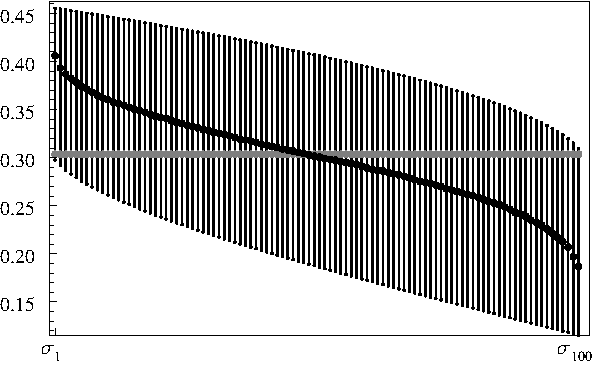
\includegraphics{figures/ch1/col_spars_nlogn_100}
\caption[Spectrum of a random submatrix of a unitary DFT matrix.]{%
{\sc Spectrum of a random submatrix of a unitary DFT matrix.}
The matrix $\mat{U}$ is a $10^2 \times
10^4$ submatrix of the unitary DFT matrix with dimension $10^4,$ and the
sampling probability $p = 10^{-4} \log(10^4).$ The $k$th vertical bar,
calculated using Theorem~\ref{ch1:thm:colsampling}, describes an interval containing
the median value of the $k$th singular value of the sampled matrix
$\widehat{\mat{U}}$. The black circles denote the empirical medians of the
singular values of $\widehat{\mat{U}}$, calculated from 500 trials. The gray
circles represent the singular values of $\E \widehat{\mat{U}}.$}  
\label{ch1:fig:nlogn}
\end{figure}

To illustrate the discriminatory power of these bounds, let $\mat{U}$ be an $n
\times n^2$ matrix consisting of $n$ rows of the $n^2 \times n^2$ Fourier matrix
and choose $p = (\log n)/n$ so that, on average, sampling reduces the aspect
ratio from $n$ to $\log n.$  For $n=100,$ we determine upper and lower bounds
for the median value of $\s_k(\widehat{\mat{U}})$ by numerically finding the
value of $\delta$ where the probability bounds in Theorem~\ref{ch1:thm:colsampling}
equal one-half. Figure \ref{ch1:fig:nlogn} plots the empirical median value along with
the computed interval. We see that these ranges reflect the behavior of the
singular values more faithfully than the simple estimates $\s_k(\mathbb{E}
\widehat{\mat{U}}) = p.$

\todo[inline]{Maybe add a section on applications where you know the eigenvectors
and the summands are sufficiently simple that can predict $\randcon(\matV)$ accurately.
In particular, spectrum of random graphs}

\section{Covariance estimation}
\label{ch1:sec:covarianceest}

We conclude with an extended example that illustrates how this circle of ideas
allows one to answer interesting statistical questions. Specifically, we
investigate the convergence of the individual eigenvalues of sample covariance
matrices. Our results establish conditions under which the eigenvalues can be
recovered to relative precision, and furthermore reflect the difference in 
the probabilities of the $k$th eigenvalue of the sample covariance matrix
over- or underestimating that of the covariance matrix.

Covariance estimation is a basic and ubiquitious problem that arises in signal
processing, graphical modeling, machine learning, and genomics, among other
areas. Let $\{\vec{\eta}_j\}_{j=1}^n \subset \R^p$ be i.i.d. samples drawn from
some distribution with zero mean and covariance matrix $\mat{C}.$ Define the
sample covariance matrix 
\[
 \widehat{\mat{C}}_n = \frac{1}{n} \sum_{j=1}^n \vec{\eta}_j\vec{\eta}_j^\star.
\]
An important challenge is to determine how many samples are needed to ensure
that the empirical covariance estimator has a fixed relative accuracy in the
spectral norm. That is, given a fixed $\varepsilon,$ how large must $n$ be so
that 
\begin{equation}
\label{ch1:eqn:relacccovar}
 \snorm{\widehat{\mat{C}}_n - \mat{C}} \leq \varepsilon \snorm{\mat{C}}?
\end{equation}

This estimation problem has been studied extensively. It is now known that for
distributions with a finite second moment, $\Omega(p \log p)$ samples suffice
\cite{RU99}, and for log-concave distributions, $\Omega(p)$ samples suffice
\cite{ALPT10b}. More broadly, Vershynin \cite{V10} conjectures that, for
distributions with finite fourth moment, $\Omega(p)$ samples suffice; he
establishes this result to within iterated log factors. In~\cite{SV11}, Srivastava
and Vershynin establish that $\Omega(p)$ samples suffice for distributions
which have finite $2+\varepsilon$ moments, for some $\varepsilon >0$, and satisfy
an additional regularity condition.

Inequality \eqref{ch1:eqn:relacccovar} ensures that the difference between the
$k$th eigenvalues of $\widehat{\mat{C}}_n$ and $\mat{C}$ is small, but it
requires $\asymO{p}$ samples to obtain estimates of even a few of the eigenvalues.
Specifically, letting $\kappa_\ell = \lambda_1(\mat{C})/\lambda_\ell(\mat{C}),$ 
we see that $\const{O}(\varepsilon^{-2} \kappa_\ell^2 p)$ samples are required to obtain
relative error estimates of the largest $\ell$ eigenvalues of $\mat{C}$ using the 
results of~\cite{ALPT10b, V10, SV11}. However, it is reasonable to expect that
when the spectrum of $\mat{C}$ exhibits decay and $\ell \ll p,$ far fewer than
$\const{O}(p)$ samples should suffice to ensure relative error recovery of the largest
$\ell$ eigenvalues. 

In fact, Vershynin shows this is the case when the random vector
is subgaussian: in~\cite{Ver10}, he defines the effective rank of $\mat{C}$ to be
$r = \big(\sum_{i=1}^p \lambda_i(\mat{C})\big) / \lambda_1(\mat{C})$
and uses $r$ to provide bounds of the form~\eqref{ch1:eqn:relacccovar}.
It follow from his arguments that, with high probability, 
the largest $\ell$ eigenvalues of $\mat{C}$ are estimated to relative precision when
$n = \const{O}(\varepsilon^{-2} r \kappa_\ell^2 \log p)$
samples are taken. Clearly this result is most of interest when
the effective rank is small: e.g. when $r$ is $\const{O}(1),$ we see that 
$\const{O}(\varepsilon^{-2} \kappa_\ell^2 \log p)$
samples suffice to give relative error accuracy in the largest $\ell$ eigenvalues of $\mat{C}.$
Note, however, that this result does not supply the rates of convergence
of the \emph{individual} eigenvalues, and it requires the effective rank to be small.
To the best of the author's knowledge, there are no nonasymptotic estimates of the 
relative errors of individual eigenvalues that do not require the 
assumption that $\mat{C}$ has low effective rank.

% In particular,
% condition \eqref{ch1:eqn:relacccovar} offers virtually no information on the
% spectrum of the estimated precision matrix $\widehat{\mat{C}}_n^{-1}.$ To obtain
% this information, one must measure the approximation error on the scale of
% $\lambdamin{\mat{C}}^{-1}.$ 

In this section, we derive a relative approximation bound for each eigenvalue of
$\mat{C}$.
For simplicity, we assume the samples are drawn from a
$\mathcal{N}(\vec{0}, \mat{C})$ distribution where $\mat{C}$ is full-rank, but
we expect that the arguments can be extended to cover other subgaussian distributions.

\begin{thm}
\label{ch1:thm:covarest}
Assume that $\mat{C} \in \samats{p}$ is positive definite. Let
$\{\vec{\eta}_j\}_{j=1}^n \subset \R^p$ be i.i.d. samples drawn from a
$\mathcal{N}(\vec{0}, \mat{C})$ distribution. Define 
\[
\widehat{\mat{C}}_n = \frac{1}{n} \sum\nolimits_{j=1}^n
\vec{\eta}_j\vec{\eta}_j^\star.
\]
Write $\lambda_k$ for the $k$th eigenvalue of $\mat{C}$, and write
$\hat{\lambda}_k$ for the $k$th eigenvalue of $\widehat{\mat{C}}_n.$ Then for
$k=1,\ldots,p,$
\begin{align*}
\Prob{\hat{\lambda}_k \geq \lambda_k + t} & \leq  (p-k+1) \cdot \exp\left(
\displaystyle \frac{-nt^2}{32 \lambda_k \sum_{i=k}^p \lambda_i} \right) \quad
\text{for } t \leq 4 n \lambda_k, \\
\intertext{ and }
\Prob{\hat{\lambda}_k \leq \lambda_k - t} & \leq  k \cdot \exp\left(
\displaystyle \frac{-3nt^2}{8 \lambda_1 \big(\lambda_1 + \sum_{i=1}^k \lambda_i
\big) } \right) \quad \text{for } t \leq n\big(\lambda_1 + \sum_{i=1}^k
\lambda_i\big).
\end{align*}

% If $k$ is an integer in $[1,n],$ then for all $t > 0,$
% \begin{equation*}
% \Prob{\lambda_k(\hat{\mat{C}}_n) \geq \lambda_k(\mat{C}) + t} \leq 
% (p - k + 1) \cdot \exp \left( \frac{-nt^2}{\left(\sum\nolimits_{i=k}^p
% \lambda_i \right)(16 \lambda_k + 4t)} \right) 
% \end{equation*}
% and 
% \begin{equation*}
% \Prob{\lambda_k(\hat{\mat{C}}_n) \leq \lambda_k(\mat{C}) - t} \leq k \cdot
% \exp\left(\frac{-nt^2}{2 \lambda_1 \left(\lambda_1 + \sum\nolimits_{i=1}^k
% \lambda_i + \tfrac{t}{3} \right)} \right).
% \end{equation*}
\end{thm}

The following corollary provides an answer to our question about relative error
estimates.
\begin{cor}
\label{ch1:cor:relerrcovarest}
Let $\lambda_k$ and $\hat{\lambda}_k$ be as in Theorem \ref{ch1:thm:covarest}. Then 
\begin{align*}
\Prob{\hat{\lambda}_k \geq (1 + \varepsilon) \lambda_k} & \leq 
(p-k+1) \cdot \exp\left(\frac{- c n \varepsilon^2 }{\sum\nolimits_{i=k}^p
\frac{\lambda_i}{\lambda_k}} \right) \quad \text{for } \varepsilon \leq 4 n, \\
\intertext{ and }
\Prob{\hat{\lambda}_k  \leq (1 - \varepsilon) \lambda_k} & \leq k \cdot
\exp\left( \frac{-c n \varepsilon^2}{\tfrac{\lambda_1}{\lambda_k}\big(
\sum_{i=1}^k \frac{\lambda_i}{\lambda_k} \big)}
\right) \quad \text{for } \varepsilon \in (0,1],
\end{align*}
where the constant $c$ is at least $1/32.$
\end{cor}

The first bound in Corollary \ref{ch1:cor:relerrcovarest} tells us how many samples
are needed to ensure that $\hat{\lambda}_k$ does not overestimate $\lambda_k.$
Likewise, the second bound tells us how many samples ensure that
$\hat{\lambda}_k$ does not underestimate $\lambda_k.$

%The first bound in Corollary \ref{ch1:cor:relerrcovarest} tells us how many samples
%are needed to ensure that $\hat{\lambda}_k$ does not appreciably overestimate
%$\lambda_k$. However, it is possible that with that many samples
%$\hat{\lambda}_k$ underestimates $\lambda_k$. Thus we say that this number of
%samples guarantees that $\hat{\lambda}_k$ is a \emph{robust underestimate} of
%$\lambda_k$: that is, $\hat{\lambda}_k$ is guaranteed to either be a genuine
%underestimate or to relatively overestimate $\lambda_k$ only slightly. Likewise,
%the second bound tells us how many samples ensure that $\hat{\lambda}_k$ does
%not appreciably underestimate $\lambda_k$. Since it is possible that with this
%many samples $\hat{\lambda}_k$ overestimates $\lambda_k$, we now interpret
%$\hat{\lambda}_k$ as a \emph{robust overestimate} of $\lambda_k.$ 

% Intuition suggests that one should need only a few samples to obtain an
% accurate upper bound on $\lambda_1$ and an accurate lower bound on $\lambda_p$.
% Corollary \ref{ch1:cor:relerrcovarest} quantifies this intuition, saying that
% $\mathrm{O}(1)$ samples are sufficient for $\hat{\lambda}_1$ and
% $\hat{\lambda}_p$ to be, respectively, a robust overestimate and a robust
% underestimate. The intuition that one needs a large number of samples to
% accurately upper bound $\lambda_p$ or lower bound $\lambda_1$ is also
% quantified: we see that $\mathrm{O}(p \log p)$ samples suffice. More generally,
% it follows from Corollary \ref{ch1:cor:relerrcovarest} that $\hat{\lambda}_k$ is a
% robust underestimate of $\lambda_k$ after $\mathrm{O}((p-k+1) \log (p-k+1) + 1)$
% observations and a robust overestimate after $\mathrm{O}(k \log k + 1)$
% observations. Consequently, $\mathrm{O}(p\log p)$ samples allow us to determine
% the full spectrum of $\mat{C}$ to within relative accuracy. 

Corollary \ref{ch1:cor:relerrcovarest} suggests that the relationship of
$\hat{\lambda}_k$ to $\lambda_k$ is determined by the spectrum of $\mat{C}$ in
the following manner. When the eigenvalues below $\lambda_k$ are small
compared with $\lambda_k$, the quantity
\[
 \sum_{i=k}^p \lambda_i/\lambda_k
\]
is small (viz., it is no larger than $p-k+1$), and so $\hat{\lambda}_k$ is not likely to overestimate $\lambda_k$.
Similarly, when the eigenvalues above $\lambda_k$ are comparable with
$\lambda_k$, the quantity
\[
\frac{\lambda_1}{\lambda_k}\left(\sum_{i=1}^k
\lambda_i/\lambda_k  \right)
\]
is small (viz., it is no larger than $k\cdot\kappa_k^2$), and so $\hat{\lambda}_k$ is not likely to underestimate $\lambda_k$.


% It is probably the case that a more refined analysis would find that the
%probability of overestimation is controlled by the ratio of \lambda_k to
%\lambda_{k-1} and that of underestimation is controlled by the ratio of
%\lambda_k to \lambda_{k+1}. I.e., only the adjacent eigenvalues affect lambda_k
% Experimentally, looks like the bound of (p \log p)/\epsilon^2 samples needed
% to ensure the sample covar of an indep Gaussian process has all eigenvalues
% within \pm\epsilon of 1 is sharp. look at bounds on wishart matrix evals for
% comparison (or NCK ineq)

\begin{remark}
The results in Theorem \ref{ch1:thm:covarest} and Corollary \ref{ch1:cor:relerrcovarest}
also apply when $\mat{C}$ is rank-deficient: simply replace each occurence of
the dimension $p$ in the bounds with $\rank(\mat{C}).$ 

Indeed, assume that $\mat{C}$ is rank-deficient and take its truncated
eigenvalue decomposition to be $\mat{C} = \mat{U} \mat{\Lambda} \mat{U}^\star.$
If $\vec{\eta}_j \sim \mathcal{N}(\vec{0}, \mat{C}),$ then $\vec{\eta}_j$ lies
in the span of $\mat{C}.$ It follows that $\hat{\lambda}_k = \lambda_k = 0$ for
all $k > \rank(\mat{C}).$ When $k \leq \rank(\mat{C}),$ we observe that  
\[
\lambda_k(\mat{C}) = \lambda_k(\mat{\Lambda}) \quad \text{ and } \quad
\lambda_k\left(\sum_j \vec{\eta}_j \vec{\eta}_j^\star \right) = \lambda_k\left(
\sum_j \vec{\xi}_j \vec{\xi}_j^\star \right),
\]
where $\vec{\xi}_j = \mat{U}^\star \vec{\eta}_j$ is distributed
$\mathcal{N}(\vec{0}, \mat{\Lambda}).$ Thus,
\[
\left| \lambda_k\left(\sum_j \vec{\eta}_j \vec{\eta}_j^\star \right) -
\lambda_k(\mat{C}) \right| =
\left| \lambda_k\left( \sum_j \vec{\xi}_j \vec{\xi}_j^\star \right) -
\lambda_k(\mat{\Lambda}) \right|.
\]
Consequently, the problem of estimating the eigenvalues of $\mat{C}$ to relative
error using the samples $\{\vec{\eta}_j\}$ is equivalent to that of estimating
the eigenvalues of the full-rank covariance matrix $\mat{\Lambda}$ to relative
error using the samples $\{\vec{\xi}_j\}.$
\end{remark}
% 
% 
% \begin{remark}
% From Corollary~\ref{ch1:cor:relerrcovarest}, we see that if $n = \Omega(
% \varepsilon^{-2} \max \{ (p-k+1)\log(p-k+1)), k \log k \} ),$ then with high
% probability $\hat{\lambda}_k$ estimates $\lambda_k$ to within a relative error
% of $\varepsilon.$ Observe that for each of the $p$ eigenvalues, the number of
% samples required to ensure relative error estimation is
% $\mathrm{O}(\varepsilon^{-2} p \log p).$ Theorem \ref{thm:examplecovarest} now
% follows from a union bound.
% \end{remark}
% 

It is reasonable to expect that one should be able to use Corollary~\ref{ch1:cor:relerrcovarest} 
to recover Vershynin's result in~\cite{Ver10} for Wishart 
matrices: that $\Omega(\varepsilon^{-2} r \kappa_\ell^2 \log p)$ samples suffice to estimate the 
eigenvalues of the covariance matrix of a Gaussian random variable to within a relative precision of 
$1 \pm \varepsilon.$ Indeed, this result follows
from Corollary~\ref{ch1:cor:relerrcovarest} and a simple union bound argument.

\begin{cor}
Assume $\mat{C}$ is positive semidefinite. Let $\{\vec{\eta}_j\}_{j=1}^n \subset
\R^p$ be i.i.d. samples drawn from a $\mathcal{N}(\vec{0}, \mat{C})$
distribution. If $n = \Omega(\varepsilon^{-2} r \kappa_\ell^2 \log p),$ then with high probability
\[
|\lambda_k(\widehat{\mat{C}}_n) - \lambda_k(\mat{C})| \leq \varepsilon
\lambda_k(\mat{C}) \quad \text{for } k=1, \ldots,\ell.
\]
\label{ch1:cor:examplecovarest}
\end{cor}

\begin{proof}
 From Corollary~\ref{ch1:cor:relerrcovarest}, we see that 
 \[
  \Prob{\lambda_k(\widehat{\mat{C}}_n) \leq (1-\varepsilon) \lambda_k} \leq p^{-\beta} 
  \quad \text{ when } n \geq 32 \varepsilon^{-2} 
  \left(\frac{\lambda_1}{\lambda_k} \sum\nolimits_{i \leq k} \frac{\lambda_i}{\lambda_k} \right)
  (\log k + \beta \log p).
 \]
Recall that $\kappa_k = \lambda_1(\mat{C})/\lambda_k(\mat{C})$ and 
$r = \big(\sum_{i=1}^p \lambda_i(\mat{C})\big)/\lambda_1(\mat{C}),$ so
\[
  \left(\frac{\lambda_1}{\lambda_k} \sum\nolimits_{i \leq k} 
   \frac{\lambda_i}{\lambda_k} \right) \leq \kappa_k^2 r.
\]
Clearly, taking $n = \Omega(\varepsilon^{-2} r \kappa_\ell^2 \log p)$ samples ensures that, 
with high probability, each of the top $\ell$ eigenvalues of the sample covariance matrix
satisfies $\lambda_k(\widehat{\mat{C}}_n) > (1 - \varepsilon)\lambda_k.$

Likewise,
\[
 \Prob{\lambda_k(\widehat{\mat{C}}_n) \geq (1-\varepsilon) \lambda_k} \leq p^{-\beta} 
 \quad \text{ when } n \geq 32 \varepsilon^{-2} 
 \left( \sum\nolimits_{i \geq k} \frac{\lambda_i}{\lambda_k} \right)
 (\log (p-k+1) + \beta \log p)
\]
and
\[
 \sum\nolimits_{i \geq k} \frac{\lambda_i}{\lambda_k} = \frac{\lambda_1}{\lambda_k} \frac{\left(\sum\nolimits_{i \geq k} \lambda_i\right)}{\lambda_1} \leq 
 \kappa_k \frac{\left(\sum\nolimits_{i=1}^p \lambda_i\right)}{\lambda_1} = \kappa_k r,
\]
so we see that taking $n = \Omega(\varepsilon^{-2} r \kappa_\ell \log p)$ samples ensures that, 
with high probability, each of the top $\ell$ eigenvalues of the sample covariance matrix 
satisfies $\lambda_k(\widehat{\mat{C}}_n) < (1 + \varepsilon)\lambda_k.$

Combining these two results, we conclude that $n = \Omega(\varepsilon^{-2} r \kappa_\ell^2 \log p)$ 
ensures that the top $\ell$ eigenvalues of $\mat{C}$ are estimated to within relative precision 
$1 \pm \varepsilon$ with probability at least $1 - 2\ell p^{-\beta}.$
\end{proof}

\subsection{Proof of Theorem \ref{ch1:thm:covarest}}
We now prove Theorem \ref{ch1:thm:covarest}. This result requires a number of
supporting lemmas; we defer their proofs until after a discussion of extensions
to Theorem \ref{ch1:thm:covarest}.

We study the error $|\lambda_k(\widehat{\mat{C}}_n) - \lambda_k(\mat{C})|.$ To
apply the methods developed in this chapter, we pass to a question about the
eigenvalues of a difference of two matrices. The first lemma accomplishes this
goal by compressing both the population covariance matrix and the sample
covariance matrix to a fixed invariant subspace of the population covariance
matrix.

\begin{lemma}
\label{ch1:lemma:splittail}
Let $\mat{X}$ be a random Hermitian matrix with dimension $p,$ and let
$\mat{A}$ be a fixed Hermitian matrix with dimension $p$. Choose $\mat{W}_+
\in \Isom{p-k+1}{p}$ and $\mat{W}_- \in \Isom{k}{p}$ for which
\[
  \lambda_k(\mat{A}) = \lambdamax{\mat{W}_+^*\mat{A}\mat{W}_+} =
\lambdamin{\mat{W}_-^*\mat{A}\mat{W}_-}.
\]
Then, for all $t >0,$
\begin{align}
 \Prob{\lambda_k(\mat{X}) \geq \lambda_k(\mat{A}) + t} & \leq
\Prob{\lambdamax{\mat{W}_+^\star \mat{X} \mat{W}_+} \geq \lambda_k(\mat{A}) + t
} \label{ch1:eqn:covardeterministicupperbnd}\\
\intertext{ and }
 \Prob{\lambda_k(\mat{X}) \leq \lambda_k(\mat{A}) -t } &\leq
\Prob{\lambdamax{\mat{W}_-^\star(\mat{A} - \mat{X}) \mat{W}_-} \geq t}.
 \label{ch1:eqn:covardeterministiclowerbnd}
\end{align}
\end{lemma}

We apply this result with $\mat{A} = \mat{C}$ and $\mat{X} =
\widehat{\mat{C}}_n.$ The first estimate \eqref{ch1:eqn:covardeterministicupperbnd}
and the second estimate \eqref{ch1:eqn:covardeterministiclowerbnd} are handled using
different arguments. The second estimate is easier because the maximum
eigenvalue of the matrix $\mat{C} - \widehat{\mat{C}}_n$ is bounded. Indeed,
\[
 \lambdamax{\mat{W}_+^\star (\mat{C} - \widehat{\mat{C}}_n) \mat{W}_+} \leq
\lambdamax{\mat{W}_+^\star \mat{C} \mat{W}_+}.
\]
Thus, we may use Theorem \ref{ch1:thm:bennett} to complete the second estimate. The
next lemma gives the matrix variances that we need to apply this theorem.

\begin{lemma}
\label{ch1:lemma:gaussiancentralsecondmoment}
Let $\vec{\xi} \sim \mathcal{N}(\mat{0}, \mat{G}).$ Then
$$
\E(\vec{\xi}\vec{\xi}^\star - \mat{G})^2 = \mat{G}^2 + \tr(\mat{G})\cdot
\mat{G}. 
$$
\end{lemma}

The first inequality \eqref{ch1:eqn:covardeterministicupperbnd} is harder because
$\widehat{\mat{C}}_n$ is unbounded. In this case, we may apply Theorem
\ref{ch1:thm:subexponentialbernstein}. To use this theorem, we need the following
moment growth estimate for rank-one Wishart matrices.

\begin{lemma}
\label{ch1:lemma:momentbound}
Let $\vec{\xi} \sim \mathcal{N}(\vec{0},\mat{G}).$ Then for any integer $m \geq
2,$
$$
\E\left(\vec{\xi}\vec{\xi}^\star \right)^m \preceq 2^m m! (\tr
\mat{G})^{m-1}\cdot \mat{G}.
$$
\end{lemma}

With these preliminaries addressed, we prove Theorem \ref{ch1:thm:covarest}.

\begin{proof}[Proof of lower estimate in Theorem~\ref{ch1:thm:covarest}]

First we consider the probability that $\hat{\lambda}_k$ underestimates
$\lambda_k$. Let $\mat{W}_- \in \Isom{k}{p}$ satisfy
\[
 \lambda_k(\mat{C}) = \lambdamin{\mat{W}_-^\star \mat{C} \mat{W}_-}.
\]
Then Lemma \ref{ch1:lemma:splittail} implies
\begin{align*}
 \Prob{\lambda_k(\widehat{\mat{C}}_n) \leq \lambda_k(\mat{C}) - t} & \leq
\Prob{\lambdamax{\mat{W}_-^\star (\mat{C} - \widehat{\mat{C}}_n) \mat{W}_-} \geq
t} \\
& = \Prob{ \lambdamax{\sum\nolimits_j \mat{W}_-^\star(\mat{C} -
\vec{\eta}_j\vec{\eta}_j^\star ) \mat{W}_-} \geq nt}.
\end{align*}
The factor $n$ comes from the normalization of the sample covariance matrix.
Each term in the sum is zero mean and bounded above by
$\mat{W}_-^*\mat{C}\mat{W}_-$ in the semidefinite order, so Theorem
\ref{ch1:thm:bennett} applies. As we desire a bound on the maximum eigenvalue of the
sum, we take $\mat{V}_+ = \mathbf{I}$ when we invoke Theorem \ref{ch1:thm:bennett}.
Then 
\[
 \sigma_1^2 = \lambdamax{ \sum\nolimits_j \E\left[\mat{W}_-^\star(\mat{C} -
\vec{\eta}_j\vec{\eta}_j^\star)\mat{W}_-\right]^2 } = n
\lambdamax{\E\left[\mat{W}_-^\star(\mat{C} -
\vec{\eta}_1\vec{\eta}_1^\star)\mat{W}_-\right]^2}.
\]
The covariance matrix of $\vec{\eta}_1$ is $\mat{C},$ so that of
$\mat{W}_-^\star \vec{\eta}_1$ is $\mat{W}_-^\star \mat{C} \mat{W}_-.$ It
follows from  Lemma \ref{ch1:lemma:gaussiancentralsecondmoment} that
\[
\E\left[\mat{W}_-^*(\mat{C} - \vec{\eta}_1\vec{\eta}_1^\star)\mat{W}_-\right]^2
= (\mat{W}_-^*\mat{C}\mat{W}_-)^2 + \tr(\mat{W}_-^*\mat{C}\mat{W}_-) \cdot
\mat{W}_-^*\mat{C}\mat{W}_-.
\]
Observe that $\mat{W}_-^*\mat{C}\mat{W}_-$ is the restriction of $\mat{C}$ to
its top $k$-dimensional invariant subspace, so
\[
 \sigma_1^2 = n \lambdamax{\E\left[\mat{W}_-^\star(\mat{C} -
\vec{\eta}_1\vec{\eta}_1^\star)\mat{W}_-\right]^2} = n\lambda_1(\mat{C}) \left(
\lambda_1(\mat{C}) + \sum_{i=1}^k \lambda_i(\mat{C}) \right) 
\]
and we can take $\randcon(\mat{V}_+) = \lambdamax{\mat{C}}.$

The subgaussian branch of the split Bernstein inequality of Theorem
\ref{ch1:thm:bennett} shows that 
\begin{equation*}
 \Prob{ \lambdamax{\sum\nolimits_j \mat{W}_-^\star(\mat{C} -
\vec{\eta}_j\vec{\eta}_j^\star ) \mat{W}_-} \geq nt} \leq 
 k \cdot \exp\left( \displaystyle \frac{-3nt^2}{8 \lambda_1(\mat{C})
\big(\lambda_1(\mat{C}) + \sum_{i=1}^k \lambda_i(\mat{C}) \big) } \right)
\end{equation*}
when  $t \leq n\big(\lambda_1(\mat{C}) + \sum_{i=1}^k \lambda_i(\mat{C})\big).$
This inequality provides the desired bound on the probability that
$\lambda_k(\widehat{\mat{C}}_n)$ underestimates $\lambda_k(\mat{C})$.
\end{proof}

\begin{proof}[Proof of upper estimate in Theorem~\ref{ch1:thm:covarest}]
Now we consider the probability that $\hat{\lambda}_k$ overestimates
$\lambda_k$. Let $\mat{W}_+ \in \Isom{p-k+1}{p}$ satisfy
\[
 \lambda_k(\mat{C}) = \lambdamax{\mat{W}_+^\star \mat{C} \mat{W}_+}.
\]
Then Lemma \ref{ch1:lemma:splittail} implies
\begin{align}
 \Prob{\lambda_k(\widehat{\mat{C}}_n) \geq \lambda_k(\mat{C}) + t} & \leq
\Prob{\lambdamax{\mat{W}_+^\star \widehat{\mat{C}}_n \mat{W}_+} \geq
\lambda_k(\mat{C}) + t} \notag \\
& = \Prob{\lambdamax{\sum\nolimits_j \mat{W}_+^\star (\vec{\eta}_j
\vec{\eta}_j^\star) \mat{W}_+} \geq n \lambda_k(\mat{C}) + n t}.
\label{ch1:eqn:upperestimateprob}
\end{align}
The factor $n$ comes from the normalization of the sample covariance matrix.

The covariance matrix of $\vec{\eta}_j$ is $\mat{C},$ so that of
$\mat{W}_+^\star \vec{\eta}_j$ is $\mat{W}_+^\star\mat{C}\mat{W}_+.$ Apply Lemma
\ref{ch1:lemma:momentbound} to verify that $\mat{W}_+^\star \vec{\eta}_j$ satisfies
the subexponential moment growth bound required by Theorem
\ref{ch1:thm:subexponentialbernstein} with 
\[
 B = 2 \tr(\mat{W}_+^*\mat{C}\mat{W}_+) \quad\text{ and }\quad \mat{\Sigma}_j^2
= 8\tr(\mat{W}_+^*\mat{C}\mat{W})\cdot \mat{W}_+^*\mat{C}\mat{W}_+.
\]
In fact, $\mat{W}_+^*\mat{C}\mat{W}_+$ is the compression of $\mat{C}$ to the
invariant subspace corresponding with its bottom $p-k+1$ eigenvalues, so 
\[
B = 2 \sum\nolimits_{i=k}^p \lambda_i(\mat{C}) \quad\text{and}\quad
\lambdamax{\mat{\Sigma}_j^2} = 8 \lambda_k(\mat{C}) \sum\nolimits_{i=k}^p
\lambda_i(\mat{C}).
\]
We are concerned with the maximum eigenvalue of the sum in
\eqref{ch1:eqn:upperestimateprob}, so we take $\mat{V}_+ = \mathbf{I}$ in the
statement of Theorem \ref{ch1:thm:subexponentialbernstein} to find that
\begin{align*}
 \sigma_1^2 & = \lambdamax{\sum\nolimits_j \mat{\Sigma}_j^2 } = n
\lambdamax{\mat{\Sigma}_1^2} = 8 n \lambda_k(\mat{C}) \sum\nolimits_{i=k}^p
\lambda_i(\mat{C}) \quad \text{and}
\\ \mu_1 & = \lambdamax{\sum_j \mat{W}_+^\star
\E(\vec{\eta}_j\vec{\eta}_j^\star) \mat{W}_+ } = n\lambdamax{\mat{W}_+^\star
\mat{C} \mat{W}_+} = n \lambda_k(\mat{C}).
\end{align*}
It follows from the subgaussian branch of the split Bernstein inequality of
Theorem \ref{ch1:thm:subexponentialbernstein} that 
$$
\Prob{\lambda_k \left(\sum\nolimits_j \mat{W}_+^\star (\vec{\eta}_j
\vec{\eta}_j^\star) \mat{W}_+ \right) \geq n \lambda_k(\mat{C}) + n t} \leq 
 (p-k+1) \cdot \exp\left( \displaystyle \frac{-nt^2}{32 \lambda_k(\mat{C})
\sum_{i=k}^p \lambda_i(\mat{C})} \right)
$$
when $t \leq 4 n \lambda_k(\mat{C}).$ This provides the desired bound on the
probability that $\lambda_k(\widehat{\mat{C}}_n)$ overestimates
$\lambda_k(\mat{C}).$
\end{proof}

\subsection{Extensions of Theorem \ref{ch1:thm:covarest}}
Results analogous to Theorem \ref{ch1:thm:covarest} can be established for other
distributions. If the distribution is bounded, the possibility that
$\hat{\lambda}_k$ deviates above or below $\lambda_k$ can be controlled using
the Bernstein inequality of Theorem \ref{ch1:thm:bennett}. If the distribution is
unbounded but has matrix moments that satisfy a sufficiently nice growth
condition, the probability that $\hat{\lambda}_k$ deviates below $\lambda_k$ can
be controlled with the Bernstein inequality of Theorem \ref{ch1:thm:bennett} and the
probability that it deviates above $\lambda_k$ can be bounded using a Bernstein
inequality analogous to that in Theorem \ref{ch1:thm:subexponentialbernstein}.

We established Theorem \ref{ch1:thm:covarest} using this technique to demonstrate
the simplicity of the Laplace transform machinery. However, the results of
\cite{ALPT10b} on the convergence of empirical covariance matrices of isotropic
log-concave random vectors lead to tighter bounds on the probability that
$\hat{\lambda}_k$ overestimates $\lambda_k.$ There does not seem to be an
analogous reduction for handling the probability that $\hat{\lambda}_k$ is an
underestimate.

To see the relevance of the results in \cite{ALPT10b}, first observe the
following consequence of the subadditivity of the maximum eigenvalue mapping:
\begin{align*}
\lambdamax{\mat{W}_+^\star(\mat{X} - \mat{A}) \mat{W}_+} & \geq
\lambdamax{\mat{W}_+^\star \mat{X} \mat{W}_+} - \lambdamax{\mat{W}_+^\star
\mat{A} \mat{W}_+} \\
 &= \lambdamax{\mat{W}_+^\star \mat{X} \mat{W}_+} - \lambda_k(\mat{A}).
\end{align*}
In conjunction with \eqref{ch1:eqn:covardeterministicupperbnd}, this gives us the
following control on the probability that $\lambda_k(\mat{X})$ overestimates
$\lambda_k(\mat{A}):$ 
\[
 \Prob{\lambda_k(\mat{X}) \geq \lambda_k(\mat{A}) + t} \leq
\Prob{\lambdamax{\mat{W}_+^\star (\mat{X} - \mat{A}) \mat{W}_+} \geq t}.
\]

In our application, $\mat{X}$ is the empirical covariance matrix and $\mat{A}$
is the actual covariance matrix. The spectral norm dominates the maximum
eigenvalue, so 
\begin{align*}
 \Prob{\lambda_k(\widehat{\mat{C}}_n) \geq \lambda_k(\mat{C}) + t} & \leq
\Prob{\lambdamax{\mat{W}_+^\star(\widehat{\mat{C}}_n - \mat{C})\mat{W}_+} \geq
t}\\
& \leq \Prob{\|\mat{W}_+^\star (\widehat{\mat{C}}_n - \mat{C}) \mat{W}_+\| \geq
t} = \Prob{\|\mat{W}_+^\star \widehat{\mat{C}}_n \mat{W}_+ - \mat{S}^2 \| \geq t
},
\end{align*}
where $\mat{S}$ is the square root of $\mat{W}_+^\star \mat{C} \mat{W}_+.$ Now
factor out $\mat{S}^2$ and identify $\lambda_k(\mat{C}) = \|\mat{S}^2\|$ to
obtain
\begin{align*}
 \Prob{\lambda_k(\widehat{\mat{C}}) \geq \lambda_k(\mat{C}) + t} & \leq
\Prob{\|\mat{S}^{-1} \mat{W}_+^\star \widehat{\mat{C}}_n \mat{W}_+ \mat{S}^{-1}
- \mathbf{I} \| \|\mat{S}^2\| \geq t } \\
 & = \Prob{\|\mat{S}^{-1} \mat{W}_+^\star \widehat{\mat{C}}_n \mat{W}_+
\mat{S}^{-1} - \mathbf{I} \| \geq t/\lambda_k(\mat{C})}.
\end{align*}
Note that if $\vec{\eta}$ is drawn from a $\mathcal{N}(\vec{0}, \mat{C})$
distribution, then the covariance matrix of the transformed sample
$\mat{S}^{-1}\mat{W}_+^\star \vec{\eta}$ is the identity:
\[
\E \left(\mat{S}^{-1}\mat{W}_+^\star \vec{\eta} \vec{\eta}^\star \mat{W}_+
\mat{S}^{-1}\right) = \mat{S}^{-1} \mat{W}_+^\star \mat{C} \mat{W}_+
\mat{S}^{-1} = \mathbf{I}.
\]
Thus $\mat{S}^{-1} \mat{W}_+^\star \widehat{\mat{C}}_n \mat{W}_+ \mat{S}^{-1}$
is the empirical covariance matrix of a standard Gaussian vector in
$\R^{p-k+1}.$ By Theorem 1 of \cite{ALPT10b}, it follows that $\hat{\lambda}_k$
is unlikely to overestimate $\lambda_k$ in relative error when the number $n$ of
samples is $\Omega(p-k+1).$

Similarly, for more general distributions, the bounds on the probability of
$\hat{\lambda}_k$ exceeding $\lambda_k$ can be tightened beyond those suggested
in Theorem \ref{ch1:thm:covarest} by using the results in \cite{ALPT10b} or
\cite{V10}.

Finally, we note that the techniques developed in the proof of Theorem
\ref{ch1:thm:covarest} can be used to investigate the spectrum of the error matrices
$\widehat{\mat{C}}_n - \mat{C}.$
\subsection{Proofs of the supporting lemmas}

We now establish the lemmas used in the proof of Theorem \ref{ch1:thm:covarest}.

\begin{proof}[Proof of Lemma \ref{ch1:lemma:splittail}]
The probability that $\lambda_k(\mat{X})$ overestimates $\lambda_k(\mat{A})$ is
controlled with the sequence of inequalities
\begin{align*}
\Prob{\lambda_k(\mat{X}) \geq \lambda_k(\mat{A}) + t} & = \Prob{ \inf_{\mat{W}
\in \Isom{p-k+1}{p}} \lambdamax{\mat{W}^*\mat{X}\mat{W}} \geq \lambda_k(\mat{A})
+ t} \\
& \leq \Prob{\lambdamax{\mat{W}_+^*\mat{X}\mat{W}_+} \geq \lambda_k(\mat{A}) +
t}. 
\end{align*}

We use a related approach to study the probability that $\lambda_k(\mat{X})$
underestimates $\lambda_k(\mat{A}).$ Our choice of $\mat{W}_-$ implies that 
\[
\lambda_{p-k+1}(-\mat{A}) = -\lambda_k(\mat{A}) =
-\lambdamin{\mat{W}_-^*\mat{A}\mat{W}_-} =
\lambdamax{\mat{W}_-^*(-\mat{A})\mat{W}_-}. 
\]
It follows that
\begin{align*}
\Prob{\lambda_k(\mat{X}) \leq \lambda_k(\mat{A}) - t} & =
\Prob{\lambda_{p-k+1}(-\mat{X}) \geq \lambda_{p-k+1}(-\mat{A}) + t} \\
& = \Prob{ \inf_{\mat{W} \in \Isom{k}{p}} \lambdamax{\mat{W}^*(-\mat{X})\mat{W}}
\geq \lambdamax{\mat{W}_-^*(-\mat{A})\mat{W}_-} + t} \\
& \leq \Prob{\lambdamax{\mat{W}_-^*(-\mat{X})\mat{W}_-} -
\lambdamax{\mat{W}_-^*(-\mat{A})\mat{W}_-} \geq t} \\
& \leq \Prob{\lambdamax{\mat{W}_-^*(\mat{A} - \mat{X})\mat{W}_-} \geq t}. 
\end{align*}
The final inequality follows from the subadditivity of the maximum eigenvalue
mapping. 
\end{proof}

\begin{proof}[Proof of Lemma \ref{ch1:lemma:gaussiancentralsecondmoment}]
We begin by taking $\mat{S}$ to be the positive-semidefinite square root of
$\mat{G}.$ Let $\mat{S} = \mat{U} \mat{\Lambda} \mat{U}^\star$ be the eigenvalue
decomposition of $\mat{S},$ and let $\vec{\gamma}$ be a $\mathcal{N}(\vec{0},
\mathbf{I}_p)$ random variable. Recalling that $\mat{G}$ is the covariance
matrix of $\mat{\xi}$, we see that $\vec{\xi}$ and $\mat{U} \mat{\Lambda}
\vec{\gamma}$ are identically distributed. Thus,
\begin{align}
\E(\vec{\xi}\vec{\xi}^\star - \mat{G})^2 
& = \E(\mat{U} \mat{\Lambda} \vec{\gamma}\vec{\gamma}^\star \mat{\Lambda}
\mat{U}^\star - \mat{U} \mat{\Lambda}^2 \mat{U}^\star)^2 \notag \\
& = \mat{U} \mat{\Lambda} \E(\vec{\gamma}\vec{\gamma}^\star \mat{\Lambda}^2
\vec{\gamma}\vec{\gamma}^\star) \mat{\Lambda} \mat{U}^\star - \mat{G}^2. 
\label{ch1:eqn:rankonewishartmatrixvarianceexpansion}
\end{align}

Consider the $(i,j)$ entry of the matrix being averaged:
\[
\E(\vec{\gamma}\vec{\gamma}^\star \mat{\Lambda}^2
\vec{\gamma}\vec{\gamma}^\star)_{ij} =  \sum_k \E(\gamma_i \gamma_j \gamma_k^2)
\lambda_k^2.
\]
The $(i,j)$ entry of this matrix is zero because the entries of $\vec{\gamma}$
are independent and symmetric. Furthermore, the $(i,i)$ entry satisfies
\[
\E(\vec{\gamma}\vec{\gamma}^\star \mat{\Lambda}^2
\vec{\gamma}\vec{\gamma}^\star)_{ii} = \E(\gamma_i^4) \lambda_i^2 + \sum_{k \neq
i} \E(\gamma_k^2) \lambda_k^2 = 2 \lambda_i^2 + \tr(\mat{\Lambda}^2).
\]
We have shown
\[
\E(\vec{\gamma} \vec{\gamma}^\star \mat{\Lambda}^2
\vec{\gamma}\vec{\gamma}^\star) = 2 \mat{\Lambda}^2 + \tr(\mat{G}) \cdot
\mathbf{I}.
\]
This equality and \eqref{ch1:eqn:rankonewishartmatrixvarianceexpansion} imply the
desired result.
\end{proof}

%\begin{proof}[Proof of Lemma \ref{ch1:lemma:gaussiancentralsecondmoment}]
%We begin by taking $\mat{G}$ to be the positive-semidefinite square root of
% $\mat{C}.$ Let $\vec{\gamma}$ be a $\mathcal{N}(\vec{0},\mathbf{I})$ random
% variable. Recalling that $\vec{\xi} \sim \mathcal{N}(\vec{0}, \mat{C}),$ we see
% that $\vec{\xi}$ and $\mat{G}\vec{\gamma}$ are identically distributed, so 
%\begin{align*} 
%\E(\vec{\xi}\vec{\xi}^\star - \mat{C})^2 & 
%= \E(\mat{G}(\vec{\gamma}\vec{\gamma}^\star - \mathbf{I})\mat{G})^2 
%= \mat{G} \E (\vec{\gamma}\vec{\gamma}^\star \mat{G}^2
% \vec{\gamma}\vec{\gamma}^\star) \mat{G} - \mat{G}^4. 
%\end{align*}
%Next, consider the $(i,j)$ entry of the matrix being averaged:
%$$
%(\vec{\gamma}\vec{\gamma}^\star \mat{G}^2 \vec{\gamma}\vec{\gamma}^\star)_{ij}
% = \sum_{kl} \gamma_i \gamma_j \gamma_k \gamma_l (\mat{G}^2)_{ij}. 
%$$
%Using the properties of standard Gaussian variables,
%$$
%\E (\gamma_i \gamma_j \gamma_k \gamma_l) = 
%\begin{cases}
%1 & \text{ if } i=j, k=l, i\neq k \\
%1 & \text{ if } i=k, j=l, i \neq j \\
%1 & \text{ if } i=l, j=k, i \neq j \\
%3 & \text{ if } i= j = k= l \\
%0 & \text{ otherwise, }
%\end{cases}
%$$
%so the $(i,j)$ entry of the matrix under consideration is
%$$
%(\vec{\gamma}\vec{\gamma}^\star \mat{G}^2 \vec{\gamma}\vec{\gamma}^\star)_{ij}
% = \delta_{ij} \left[ 3 (\mat{G}^2)_{ij} + \sum_{k \neq i} (\mat{G}^2)_{kk}
% \right] + (1 - \delta_{ij})[ (\mat{G}^2)_{ij} + (\mat{G}^2)_{ji} ] = 2
% (\mat{G}^2)_{ij} + \tr \mat{G}^2.
%$$
%Therefore, 
%\begin{align*} 
%\E(\vec{\xi}\vec{\xi}^\star - \mat{C})^2 
%= \mat{G} \E (\vec{\gamma}\vec{\gamma}^\star \mat{G}^2
% \vec{\gamma}\vec{\gamma}^\star) \mat{G} - \mat{G}^4 = \mat{C}^2 + \tr(\mat{C})
% \mat{C}.
%\end{align*}
%This is the desired expression for the matrix variance of a rank-one Wishart
% matrix.
%\end{proof}

\begin{proof}[Proof of Lemma \ref{ch1:lemma:momentbound}]

Factor the covariance matrix of $\vec{\xi}$ as $\mat{G} = \mat{U\Lambda
U}^\star$ where $\mat{U}$ is orthogonal and $\mat{\Lambda} =
\text{diag}(\lambda_1, \ldots, \lambda_p)$ is the matrix of eigenvalues of
$\mat{G}$. Let $\vec{\gamma}$ be a $\mathcal{N}(\vec{0},\mathbf{I}_p)$ random
variable. Then $\vec{\xi}$ and $\mat{U\Lambda}^{1/2} \vec{\gamma}$ are
identically distributed, so 
\begin{align} 
\E (\vec{\xi}\vec{\xi}^\star)^m & = \E\left[(\vec{\xi}^\star\vec{\xi})^{m-1}
\vec{\xi}\vec{\xi}^\star \right] = \E\left[ (\vec{\gamma}^\star \mat{\Lambda}
\vec{\gamma})^{m-1} \mat{U\Lambda}^{1/2} \vec{\gamma}\vec{\gamma}^\star
\mat{\Lambda}^{1/2} \mat{U}^\star \right]\notag \\
 & = \mat{U\Lambda}^{1/2} \E \left[ (\vec{\gamma}^\star \mat{\Lambda}
\vec{\gamma})^{m-1} \vec{\gamma}\vec{\gamma}^\star \right]
\mat{\Lambda}^{1/2}\mat{U}^\star. 
\label{ch1:eqn:rankonewishartpowers}
\end{align}
Consider the $(i,j)$ entry of the bracketed matrix in
\eqref{ch1:eqn:rankonewishartpowers}:
\begin{equation}
\E\left[(\vec{\gamma}^\star \mat{\Lambda} \vec{\gamma})^{m-1} \gamma_i\gamma_j
\right] = \E\left[\left(\sum\nolimits_{\ell=1}^p \lambda_\ell \gamma_\ell^2
\right)^{m-1} \gamma_i \gamma_j\right]. 
\label{ch1:eqn:gaussianchaos}
\end{equation}
From this expression, and the independence and symmetry of the Gaussian variables $\{
\gamma_i \},$ we see that this matrix is diagonal.

To bound the diagonal entries, use a multinomial expansion to further develop
the sum in \eqref{ch1:eqn:gaussianchaos} for the $(i,i)$ entry:
\[
 \E\left[(\vec{\gamma}^\star \mat{\Lambda} \vec{\gamma})^{m-1} \gamma_i^2
\right]  
= \sum_{\ell_1 + \cdots +\ell_p = m-1} \binom{m-1}{\ell_1, \ldots, \ell_p}
\lambda_1^{\ell_1} \cdots \lambda_p^{\ell_p} \E\left[\gamma_1^{2\ell_1}
\cdots \gamma_p^{2\ell_p} \gamma_i^2 \right].
\]
Now we use the generalized AM--GM inequality to replace the expectation of the
product of Gaussians with the $2m$th moment of a single standard Gaussian $g$. 
Denote the $L_r$ norm of a random variable $X$ by
\[ 
  \lnorm{r}{X} = \left(\E |X|^r \right)^{1/r}. 
\]
Since $\ell_1, \ldots, \ell_p$ are nonnegative integers summing to $m-1$, the
generalized AM-GM inequality justifies the first of the following inequalities:
\begin{align*}
\E \gamma_1^{2\ell_1} \cdots \gamma_p^{2\ell_p} \gamma_i^2 & \leq  \E
\left(\frac{\ell_1 |\gamma_1| + \cdots + \ell_p |\gamma_p| +
|\gamma_i|}{m}\right)^{2m} =
 \lnorm{2m}{ \frac{1}{m} \left(|\gamma_i| + \sum_{j=1}^p \ell_j |\gamma_j|
\right) }^{2m} \\
 & \leq \left( \frac{1}{m} \left( \lnorm{2m}{\gamma_i} + \sum_{j=1}^p \ell_j
\lnorm{2m}{\gamma_j} \right) \right)^{2m} \\
 & = \left(\frac{1 + \ell_1 + \ldots + \ell_p}{m} \right)^{2m}
\lnorm{2m}{g}^{2m} = \E (g^{2m}).  
\end{align*}
The second inequality is the triangle inequality for $L_r$ norms. Now we reverse
the multinomial expansion to see that the diagonal terms satisfy the inequality
\begin{align}
\E\left[(\vec{\gamma}^\star \mat{\Lambda} \vec{\gamma})^{m-1}\gamma_i^2\right] &
\leq \sum_{\ell_1 + \cdots + \ell_p = m-1} \binom{m-1}{\ell_1, \ldots,
\ell_p } \lambda_1^{\ell_1} \cdots \lambda_p^{\ell_p} \E (g^{2m}) \notag
\\
&  = (\lambda_1 + \ldots + \lambda_p)^{m-1}\E ( g^{2m}) = \tr(\mat{G})^{m-1} \E
(g^{2m}). 
\label{ch1:eqn:diagonalest}
\end{align}
Estimate $\E(g^{2m})$ using the fact that $\Gamma(x)$ is increasing for $x \geq
1:$
\begin{align*}
\E \left( g^{2m} \right) & = \frac{2^m}{\sqrt{\pi}} \Gamma(m + 1/2) <
\frac{2^m}{\sqrt{\pi}} \Gamma(m+1) = \frac{2^m}{\sqrt{\pi}} m! \quad \text{for }
m \geq 1.
\end{align*}
Combine this result with \eqref{ch1:eqn:diagonalest} to see that
\[
\E\left[(\vec{\gamma}^\star \mat{\Lambda}
\vec{\gamma})^{m-1}\vec{\gamma}\vec{\gamma}^\star \right] \preceq
\frac{2^m}{\sqrt{\pi}} m! \tr(\mat{G})^{m-1} \cdot \mathbf{I}. 
\] 
Complete the proof by using this estimate in \eqref{ch1:eqn:rankonewishartpowers}.
\end{proof}

% \begin{lemma}
% \label{lemma:bernsteinmomentbound}
% Let $\mat{X}$ be a random $n \times n$ Hermitian matrix such that for some
% positive semidefinite $\mat{\sigma}^2$ and some constant $M \in (0, \infty),$
% \begin{equation}
% \E \mat{X}^k \preceq \frac{k!}{2} \mat{\sigma}^2 M^{k-2} \quad \text{for } k
% \geq 2. 
% \label{eqn:bernsteinmomentbound}
% \end{equation}
% Then 
% $$
% \E \exp(\theta \mat{X}) \preceq \exp\left(\theta \E\mat{X} + \frac{\theta^2
% \mat{\sigma}^2}{2-2M\theta}\right) \quad \text{for } 0 \leq M\theta < 1.
% $$
% \end{lemma}
%!TEX root = thesis.tex

\chapter{Randomized sparsification in \protect{\textsc{NP}}-hard norms}
\label{ch2}

\todo[inline]{Incorporate referees' comments}
\todo[inline]{Desperately search for applications!}
\todo[inline]{Note that Nguyen et al. developed spectral bound for sparsification. See how compares to ours}
\todo[inline]{Applications to Max-cut a la~\cite{DKM08}?}
\todo[inline]{Use subgaussianity to get tail bounds?}

Massive matrices are ubiquitous in modern data processing. Classical dense
matrix algorithms are poorly suited to such problems because their running times
scale superlinearly with the size of the matrix. When the dataset is sparse, one
prefers to use sparse matrix algorithms, whose running times depend more on the
sparsity of the matrix than on the size of the matrix. Of course, in many
applications the matrix is \emph{not} sparse. Accordingly, one may wonder
whether it is possible to approximate a computation on a large dense matrix with
a related computation on a sparse approximant to the matrix.

Let $\|\cdot\|$ be a norm on matrices. Here is one way to frame this challenge 
mathematically: Given a matrix $\mat{A}$, how can one efficiently generate a sparse matrix
$\mat{X}$ for which the approximation error $\|\mat{A} - \mat{X}\|$ is small? 

The literature has concentrated on the behavior of the approximation error in
the spectral and Frobenius norms; however, these norms are not always the most
natural choice. Sometimes it is more appropriate to consider the matrix as an operator
from a finite-dimensional $\ell_p$ space to a finite-dimensional $\ell_q$
space, and investigate the behavior of the approximation error in the associated
$p \rightarrow q$ operator norm. As an example, the problem of graph sparsification is naturally
posed as a question of preserving the so-called \emph{cut norm} of a matrix associated 
with the graph. The strong equivalency of the cut norm and the $\infone$ norm suggests that, for
graph-theoretic applications, it may be fruitful to consider the behavior of the
$\infone$ norm under sparsification. In other applications, e.g., the column
subset selection algorithm in \cite{Tropp09}, the $\inftwo$ norm is the norm of
interest.

This chapter investigates the errors incurred by approximating a fixed real matrix
with a random matrix\footnote{The content of this chapter is adapted from the 
technical report~\cite{GT11} co-authored with Joel Tropp.}. Our results apply to any 
scheme in which the entries of the approximating matrix are independent and average 
to the corresponding entries of the fixed matrix. Our main contribution is a bound 
on the expected $\infp$ norm error, which we specialize to the case of the $\infone$ 
and $\inftwo$ norms. We also use a result of Lata{\l}a~\cite{Lat04} to bound
the expected spectral approximation error, and we establish the
subgaussianity of the spectral approximation error.

% \subsection{Outline}
% 
% Section \ref{ch2:sec:literature} offers an overview of the related strands of
% research, and Section \ref{ch2:sec:background} introduces the reader to our
% notations. In Section \ref{ch2:sec:inftopbound}, we establish the foundations for
% our $\infone$ and $\inftwo$ error estimates: an estimate of the expected $\infp$
% norm of a random matrix with independent, zero-mean entries and a tail bound for
% this quantity. In Sections \ref{ch2:sec:inf1norm} and \ref{ch2:sec:inf2norm}, these
% estimates are specialized to the cases $p=1$ and $p=2$, respectively, and we
% establish the optimality of the resulting expressions. The bounds are provided
% in both their most generic forms and ones more suitable for applications. In
% Section \ref{ch2:sec:spectralerrbound}, we use a result due to Lata\l{}a
% \cite{Lat04} to find an optimal estimate of the spectral approximation error. A
% deviation bound is provided for the spectral norm which captures the correct
% (subgaussian) tail behavior. We show that our estimates applied to the
% sparsification schemes in \cite{
% AHK06} and \cite{AM07} recover performance guarantees comparable with those
% obtained from the original analyses, under slightly weaker hypotheses.

% 
% \section{Related Work}
% \label{ch2:sec:literature}
% 
% In recent years, much attention has been paid to the problem of using sampling
% methods to approximate linear algebra computations efficiently. Such algorithms
% find applications in areas like data mining, computational biology, and other
% areas where the relevant matrices may be too large
% to fit in RAM, or large enough that the computational requirements of standard
% algorithms become prohibitive. Here we review the streams of literature that
% have motivated and influenced this work.
% 
% \subsection{Randomized sparsification}
% 
% \subsection{Probability in Banach spaces}

Our methods are similar to those of Rudelson and Vershynin in \cite{RV07} in
that we treat $\mat{A}$ as a linear operator between finite-dimensional
Banach spaces and use some of the same tools of probability in Banach spaces.
Whereas Rudelson and Vershynin consider the behavior of the norms of random
submatrices of $\mat{A}$, we consider the behavior of the norms of matrices
formed by randomly sparsifying (or quantizing) the entries of $\mat{A}$. This
yields error bounds applicable to schemes that sparsify or quantize matrices
entrywise. Since some graph algorithms depend more on the number of edges in the
graph than the number of vertices, such schemes may be useful in developing
algorithms for handling large graphs.
% 
% \subsection{Random sampling of graphs}
% 
% The bulk of the literature has focused on the behavior of the spectral and
% Frobenius norms under randomized sparsification, but the $\infone$ norm occurs
% naturally in connection with graph theory. Let us review the relevant ideas.
In particular, the algorithm of~\cite{BSS08} is not suitable for sparsifying graphs
with a large number of vertices. Part of our motivation for investigating the
$\infone$ approximation error is the belief that the equivalence of the cut norm
with the $\infone$ norm means that matrix sparsification in the $\infone$ norm
might be useful for efficiently constructing optimal sparsifiers for such
graphs.


\section{Notation}
We establish the notation particular to this chapter.

All quantities are real. For $1\leq p\leq\infty$, the $\ell_p^n$ norm of $\vec{x} \in \R^n$ is written as
$\pnorm{\mat{x}}$. Each space $\ell_p^n$ has an associated dual space $\ell_{p^\prime}^n,$ where
$p^\prime,$ the \emph{conjugate exponent} to $p,$ is determined by the relation $p^{-1} + (p^\prime)^{-1} = 1.$ 
The dual space of $\ell_1^n$ (respectively, $\ell_\infty^n$) is 
$\ell_\infty^n$ (respectively, $\ell_1^n$).

The $k$th column of the matrix $\mat{A}$ is denoted by $\matA_{(k)},$ and the $(j,k)$th element is 
denoted by $a_{jk}.$ We treat $\mat{A}$ as an operator from $\ell_{p}^{n}$ to
$\ell_{q}^{m}$, and the $p\rightarrow q$ operator norm of $\mat{A}$ is written
as $\norm{\mat{A}}_{p\rightarrow q}$. The spectral norm, i.e.\ the $2 \rightarrow 2$ operator norm, is written
$\TNorm{\matA}.$ Recall that given an operator $\matA : \ell_{p}^{n} \rightarrow \ell_q^{m},$
the associated adjoint operator ($\matA\transp,$ in the case of a matrix) maps
from $\ell_{q^\prime}^{m}$ to $\ell_{p^\prime}^{n}.$ Further, the $p\rightarrow q$ and $q^{\prime}
\rightarrow p^{\prime}$ norms are dual in the sense that 
\[
\norm{\mat{A}}_{p\rightarrow q}=\norm{\mat{A}^{T}}_{q^{\prime}\rightarrow
p^{\prime}}.
\]

This chapter is concerned primarily with the spectral norm and the $\infone$ and
$\inftwo$ norms. The $\infone$ and $\inftwo$ norms are not unitarily invariant, so 
do not have simple interpretations in terms of singular values; in fact, they are
\textsc{NP}-hard to compute for general matrices~\cite{Rohn00}. 
We remark that $\infonorm{\mat{A}}=\norm{\mat{A}\mat{x}}_{1}$ and
$\inftnorm{\mat{A}}=\norm{\mat{A}\mat{y}}_{2}$ for certain vectors $\mat{x}$ and
$\mat{y}$ whose components take values $\pm1$. An additional operator norm, the $\twoinf$ norm, is of interest: it is the
largest $\ell_{2}$ norm achieved by a row of $\mat{A}$. In the sequel we
also encounter the column norm 
\[
\colnorm{\mat{A}}=\sum\nolimits_k\|\matA_{(k)}\|_{2}.
\]

The variance of $X$ is written $\var{X} = \E(X-\E X)^2$. The expectation taken with respect to one
variable $X$, with all others fixed, is written $\E_X$. 
The expression $X \sim Y$ indicates the random variables $X$ and $Y$ are
identically distributed. Given a random variable $X$, the symbol $X^\prime$
denotes a random variable independent of $X$ such that $X^\prime \sim X$. The
indicator variable of the event $X > Y$ is written $\mathds{1}_{X > Y}$.
The Bernoulli distribution with expectation $p$ is written $\text{Bern}(p)$ and
the binomial distribution of $n$ independent trials each with success
probability $p$ is written $\text{Bin}(n,p)$. We write $X \sim \text{Bern}(p)$
to indicate $X$ is Bernoulli with mean $p.$

\subsubsection{Graph sparsification}

Graphs are often represented and fruitfully manipulated in terms of matrices,
so the problems of graph sparsification and matrix sparsification are strongly related.
We now introduce the relevant notation before surveying the literature.

Let $G=(V,E,\omega)$ be a weighted simple undirected graph with $n$ vertices, $m$ edges,
and adjacency matrix $\mat{A}$ given by
\[
 a_{jk} = \begin{cases} 
           \omega_{jk} & (j,k) \in E \\
           0 & \text{ otherwise}
          \end{cases}.
\]
Orient the edges of $G$ in an arbitrary manner. Then define the corresponding
$2m \times n$  \emph{oriented incidence matrix} $\mat{B}$ in the following manner: 
$b_{2i-1,j} = b_{2i, k} = \omega_i$ and $b_{2i-1,k} = b_{2i, j} = -\omega_i$ if 
edge $i$ is oriented from vertex $j$ to vertex $k,$ and all other entries of 
$B$ are identically zero.

A \emph{cut} is a partition of the vertices of $G$ into two blocks:
$V=S\cup\overline{S}$. The \emph{cost} of a cut is the sum of the weights of all
edges in $E$ which have one vertex in $S$ and one vertex in
$\overline{S}$.
Several problems relating to cuts are of considerable practical interest. In
particular, the \textsc{maxcut} problem, to determine the cut of maximum cost in
a graph, is common in computer science applications. The cuts of maximum cost
are exactly those that correspond to the \emph{cut-norm} of the oriented incidence matrix
$\mat{B}$, which is defined as 
\[
\cutnorm{\mat{B}}=\max_{I \subset \{1,\ldots,2m\},\, J \subset \{1,\ldots,n\}} 
\left| \sum\nolimits_{i \in I, j \in J} b_{ij} \right|.
\]
Finding the cut-norm of
a general matrix is \textsc{NP}-hard, but in~\cite{AN04}, the authors offer a
randomized polynomial-time algorithm which finds a submatrix $\tilde{\mat{B}}$
of $\mat{B}$ for which $|\sum_{jk}\tilde{b}_{jk}|\geq0.56\cutnorm{\mat{B}}$. This
algorithm thereby gives a feasible means of approximating the \textsc{maxcut}
value for arbitrary graphs. A crucial point in the derivation of the algorithm is 
the fact that for general matrices the $\infone$ operator norm is strongly equivalent 
with the cut-norm: 
\[
\cutnorm{\mat{A}}\leq\infonorm{\mat{A}}\leq4\cutnorm{\mat{A}};
\]
in fact, in the particular case of oriented incidence matrices, 
$\cutnorm{\mat{B}} = \infonorm{\mat{B}}.$

In his thesis~\cite{Kar95th} and the sequence of papers~\cite{Kar94a,Kar94b,Kar96}, 
Karger introduces the idea of random sampling to
increase the efficiency of calculations with graphs, with a focus on cuts. 
In~\cite{Kar96}, he shows that by picking each edge of the graph with a probability
inversely proportional to the density of edges in a neighborhood of that edge,
one can construct a \emph{sparsifier}, i.e., a graph with the same vertex set
and significantly fewer edges that preserves the value of each cut to within a
factor of $(1\pm\epsilon)$.

In \cite{SS08}, Spielman and Srivastava improve upon this sampling scheme,
instead keeping an edge with probability proportional to its \emph{effective
resistance}---a measure of how likely it is to appear in a random spanning tree
of the graph. They provide an algorithm which produces a sparsifier with
$\asymO{(n\log n)/\epsilon^{2}}$ edges, where $n$ is the number of vertices in
the graph. They obtain this result by reducing the problem to the behavior of
projection matrices $\mat{\Pi}_{G}$ and $\mat{\Pi}_{G^{\prime}}$ associated with the
original graph and the sparsifier, and then appealing to a spectral-norm
concentration result.

The $\log n$ factor in \cite{SS08} seems to be an unavoidable consequence of
using spectral-norm concentration. In \cite{BSS08}, Batson et al. prove that
the $\log n$ factor is not intrinsic: they establish that every graph has a
sparsifier that has $\Omega(n)$ edges. The existence proof is constructive and provides a
deterministic algorithm for constructing such sparsifiers in
$\const{O}(n^3m)$ time, where $m$ is the number of edges in the original graph.

\section{Preliminaries}

Bounded differences inequalities are useful tools for establishing measure 
concentration for functions of independent random variables that are insensitive
to changes in a single argument. In this chapter, we use a 
bounded differences inequality to show that the norms of the random matrices
that we encounter exhibit measure concentration.

Before stating the inequality of interest to us, we 
establish some notation. Let $g:\R^{n}\rightarrow\R$ be a measurable
function of $n$ random variables. Let $X_{1},\ldots,X_{n}$ be independent random
variables, and write $W=g(X_{1},\ldots,X_{n})$. Let $W_i$ denote the random
variable obtained by replacing the $i$th argument of $g$ with an independent
copy: $W_{i}=g(X_{1},\dots,X_{i}^{\prime},\ldots,X_{n})$. 

The following bounded differences inequality states that if $g$ is insensitive
to changes of a single argument, then $W$ does not deviate much from its mean.
\begin{lemma}[\protect{\cite[Corollary 3]{BLM03}}]
Let $W$ and $\{W_i\}$ be random variables defined as above. Assume that there
exists a positive number $C$ such that, almost surely, 
\[
\sum\nolimits_{i=1}^{n}(W-W_{i})^{2}\mathds{1}_{W>W_{i}}\leq C.
\]
Then, for all $t>0,$
\[
\Prob{W>\E W+t}\leq \e^{-t^{2}/(4C)}.
\]
\label{ch2:lem:logsob}
\end{lemma}

Rademacher random variables take the values $\pm 1$ with equal
probability. Rademacher vectors are vectors of i.i.d.\ Rademacher random
variables. We make use of Rademacher variables in this chapter to simplify our analyses 
through the technique of Rademacher symmetrization. Essentially, given
 a random variable $Z,$ Rademacher symmetrization allows us to estimate the behavior
 of $Z$ in terms of that of the random variable $Z_\text{sym} = \varepsilon(Z - Z^\prime),$
 where $Z^\prime$ is an i.i.d. copy of $Z$ and $\varepsilon$ is a Rademacher
 random variable that is independent of the pair $(Z, Z^\prime).$ The variable
 $Z_\text{sym}$ is often easier to manipulate than $Z,$ since it is guaranteed
  to be symmetric (i.e., $Z_\text{sym}$ and $-Z_\text{sym}$ are identically distributed);
  in particular, $\E Z_\text{sym}=0.$ The following
basic symmetrization result is drawn from \cite[Lemma
2.3.1 et seq.]{vdVW}.

\begin{lemma}
Let $Z_1, \ldots, Z_n, Z_1^\prime, \ldots, Z_n^\prime$ be independent random
variables satisfying $Z_i \sim Z_i^\prime$, and let $\boldsymbol{\varepsilon}$
be a Rademacher vector. Let $\mathcal{F}$ be a family of functions such that 
\[
\sup_{f \in \mathcal{F}} \sum\nolimits_{k=1}^n (f(Z_k) - f(Z_k^\prime))
\]
is measurable. Then 
\[
\E \sup_{f \in \mathcal{F}} \sum\nolimits_{k=1}^n (f(Z_k) - f(Z_k^\prime)) = \E
\sup_{f \in \mathcal{F}} \sum\nolimits_{k=1}^n \varepsilon_k (f(Z_k) -
f(Z_k^\prime)).
\]
\label{ch2:lem:symmetrization}
\end{lemma}
Since we work with finite-dimensional probability models and linear functions,
measurability concerns can be ignored in our applications of Lemma~\ref{ch2:lem:symmetrization}.

While Lemma~\ref{ch2:lem:symmetrization} allows us to replace certain 
random processes with Rademacher processes, Talagrand's Rademacher comparison 
theorem~\cite[Theorem 4.12 et seq.]{LT91} shows that certain 
complicated Rademacher processes are bounded by simpler Rademacher processes.
Together, these two results often allow us to reduce the analysis of complicated
random processes to the analysis of simpler Rademacher processes. 

\begin{lemma}
Fix finite-dimensional vectors $\mat{z}_{1},\ldots,\mat{z}_{n}$ and let
$\boldsymbol{\varepsilon}$ be a Rademacher vector. Then \[
\E\supoverqball\sum\nolimits_{k=1}^{n}\varepsilon_k|\langle\mat{z}_{k},\mat{u}
\rangle|\leq\E\supoverqball\sum\nolimits_{k=1}^{n}\varepsilon_{k}\langle\mat{z}_
{k},\mat{u}\rangle.\]
 \label{ch2:lem:comparison}
\end{lemma}

Lemma~\ref{ch2:lem:comparison} involves Rademacher sums, i.e.\ sums of the form
$\sum_k \varepsilon_k x_k$ where $\boldsymbol{\varepsilon}$ is a Rademacher
vector and $\vec{x}$ is a fixed vector. One of the most basic tools for understanding 
Rademacher sums is the Khintchine 
inequality~\cite{Szarek78}, which gives information on the moments of a Rademacher 
sum; in particular, it tells us
the expected value of the sum is equivalent with the $\ell_2$ norm of the vector
$\mat{x}$.

%allows us to bound the expected value of the sum, both above and below, with
%the $\ell_2$ norm of $\mat{x}$:
\begin{lemma}[Khintchine Inequality]
Let $\mat{x}$ be a real vector, and let $\boldsymbol{\varepsilon}$ be a
Rademacher vector. Then 
\[
\frac{1}{\sqrt{2}}\norm{\mat{x}}_{2}\leq\E\left|\sum\nolimits_{k}\varepsilon_{k}
x_{k}\right|\leq\norm{\mat{x}}_{2}.
\]
\label{chprelim:lem:khintchine}
\end{lemma}
In its more general form, which we do not use in this thesis, the Khintchine 
inequality implies that Rademacher sums are subguassian random variables.


\section{The $\infp$ norm of a random matrix}
\label{ch2:sec:inftopbound}

We are interested in schemes that approximate a given matrix $\mat{A}$ by means
of a random matrix $\mat{X}$ in such a way that the entries of $\mat{X}$ are
independent and $\E\mat{X} = \mat{A}$. It follows that the error matrix
$\mat{Z}=\mat{A}-\mat{X}$ has independent, zero-mean entries. Ultimately 
we aim to construct $\mat{X}$ so that it has the property that, with high probability,
many of its entries are identically zero, but this property does not play
a role at this stage of the analysis.

In this section, we derive a bound on the expected value of the $\infp$ norm of
a random matrix with independent, zero-mean entries. We also study the tails of
this error. In the next two sections, we use the results of this section to
reach more detailed conclusions on the $\infone$ and $\inftwo$ norms of
$\mat{Z}$.

\subsection{The expected $\infp$ norm} 
The main tools used to derive the bound on the
expected norm of $\mat{Z}$ are Lemma~\ref{ch2:lem:symmetrization},
a result on the Rademacher symmetrization of random processes, and 
Lemma~\ref{ch2:lem:comparison}, Talagrand's Rademacher comparison theorem.

We now state and prove the bound on the expected norm of $\mat{Z}$.
\begin{thm}
Let $\mat{Z}$ be a random matrix with independent, zero-mean entries and let
$\boldsymbol{\varepsilon}$ be a Rademacher vector independent of $\mat{Z}$. Then
\[
\E\norm{\mat{Z}}_{\infty\rightarrow p} \leq 2\E\pnorm{\sum\nolimits_k
\varepsilon_k \mat{Z}_{(k)}} + 2 \supoverqball \E\sum\nolimits_k
\left|\sum\nolimits_j \varepsilon_j Z_{jk} u_j \right|
\]
where $q$ is the conjugate exponent of $p$.
\label{ch2:thm:inftopbound}
\end{thm}

\begin{proof}[Proof of Theorem \ref{ch2:thm:inftopbound}] 
By duality, 
\[
\E\norm{\mat{Z}}_{\infty\rightarrow
p}=\E\norm{\mat{Z}^{T}}_{q\rightarrow1}=\E\supoverqball\sum\nolimits
_{k}|\langle\mat{Z}_{(k)},\mat{u}\rangle|.
\]
Center the terms in the sum and apply subadditivity of the maximum to get
\begin{equation}
\begin{aligned}
\E\norm{\mat{Z}}_{\infty\rightarrow p} &
\leq\E\supoverqball\sum\nolimits_{k}(|\langle\mat{Z}_{(k)},\mat{u}
\rangle|-\E^\prime|\langle\mat{Z}_{(k)}^\prime,\mat{u}
\rangle|)+\supoverqball\E\sum\nolimits_{k}|\langle\mat{Z}_{(k)},\mat{u}\rangle| \\
	& = F+S.
\end{aligned}
\label{ch2:eqn:infpexpression}
\end{equation}

Begin with the first term on the right-hand side of \eqref{ch2:eqn:infpexpression}. Use Jensen's inequality
to draw the expectation outside of the maximum: 
\[
F\leq\E\supoverqball\sum\nolimits_{k}(|\langle\mat{Z}_{(k)},\mat{u}
\rangle|-|\langle\mat{Z}_{(k)}^{\prime},\mat{u}\rangle|).
\]
Now apply Lemma~\ref{ch2:lem:symmetrization} to symmetrize the random
variable: 
\[
F\leq\E\supoverqball\sum\nolimits_{k}\varepsilon_{k}(|\langle\mat{Z}_{(k)},\mat{u}
\rangle|-|\langle\mat{Z}_{(k)}^{\prime},\mat{u}\rangle|).
\]
By the subadditivity of the maximum, \[
F\leq\E\left(\supoverqball\sum\nolimits_{k}\varepsilon_{k}|\langle\mat{Z}_{(k)},
\mat{u}\rangle|+\supoverqball\sum\nolimits_{k}-\varepsilon_{k}|\langle\mat{Z}_{(k)},
 \mat{u}\rangle|\right)=2\E\supoverqball\sum\nolimits_{k}\varepsilon_{k}
|\langle\mat{Z}_{(k)},\mat{u}\rangle|,
\]
where we have invoked the fact that $-\varepsilon_{k}$ has the Rademacher
distribution. Apply Lemma~\ref{ch2:lem:comparison} to get the final estimate
of $F$: 
\[
F\leq2\E\supoverqball\sum\nolimits_{k}\varepsilon_{k}\langle\mat{Z}_{(k)},\mat{u}
\rangle=2\E\supoverqball\left\langle
\sum\nolimits_{k}\varepsilon_{k}\mat{Z}_{(k)},\mat{u}\right\rangle
=2\E\norm{\sum\nolimits_{k}\varepsilon_{k}\mat{Z}_{(k)}}_{p}.
\]

Now consider the last term on the right-hand side of \eqref{ch2:eqn:infpexpression}. Use Jensen's
inequality to prepare for symmetrization: 
\[
\begin{split}
S &
=\supoverqball\E\sum\nolimits_{k}\left|\sum\nolimits_{j}Z_{jk}u_{j}
\right|=\supoverqball\E\sum\nolimits_{k}\left|\sum\nolimits_{j}(Z_{jk}-\E^\prime
Z_{jk}^\prime)u_{j}\right|\\
 &
\leq\supoverqball\sum\nolimits_{k}\E\left|\sum\nolimits_{j}(Z_{jk}-Z_{jk}^{
\prime})u_{j}\right|.
\end{split}
\]
Apply Lemma~\ref{ch2:lem:symmetrization} to the expectation of the inner sum
to see
\[
S\leq\supoverqball\sum\nolimits_{k}\E\left|\sum\nolimits_{j}\varepsilon_{j}(Z_{
jk}-Z_{jk}^{\prime})u_{j}\right|.
\]
The triangle inequality gives us the final expression:
\[
S\leq\supoverqball2\E\sum\nolimits_{k}\left|\sum\nolimits_{j}\varepsilon_{j}Z_{
jk}u_{j}\right|.
\]
Introduce the bounds for $F$ and $S$ into \eqref{ch2:eqn:infpexpression} to complete
the proof.
\end{proof}

\subsection{A tail bound for the $\infp$ norm}
We now develop a deviation bound for the $\infp$ approximation error. The
argument is based on Lemma~\ref{ch2:lem:logsob}, a bounded differences inequality.

To apply Lemma~\ref{ch2:lem:logsob}, we let $\mat{Z}=\mat{A}-\mat{X}$ be our
error matrix, $W=\norm{\mat{Z}}_{\infty\rightarrow p}$, and
$W^{jk}=\norm{\mat{Z}^{jk}}_{\infty\rightarrow p}$, where $\mat{Z}^{jk}$ is a
matrix obtained by replacing $a_{jk}-X_{jk}$ with an identically
distributed variable $a_{jk}-X_{jk}^{\prime}$ while keeping all other variables
fixed. The $\infp$ norms are sufficiently insensitive to each entry of the
matrix that Lemma~\ref{ch2:lem:logsob} gives us a useful deviation bound.

\begin{thm}
Fix an $m \times n$ matrix $\mat{A}$, and let $\mat{X}$ be a random matrix with
independent entries for which $\E X = \mat{A}$. Assume
$\left|X_{jk}\right|\leq\frac{D}{2}$ almost surely for all $j,k$. Then, for all
$t>0$,
\[
\Prob{\norm{\mat{A}-\mat{X}}_{\infty\rightarrow p}>
\E\norm{\mat{A}-\mat{X}}_{\infty\rightarrow p}+t}\leq \e^{-t^{2}/(4D^{2}nm^{s})}
\]
where $s=\max\{0, 1-2/q\}$ and $q$ is the conjugate exponent to $p$. 
\label{ch2:thm:inftopnormdevbnd}
\end{thm}

\begin{proof}
Let $q$ be the conjugate exponent of $p$, and choose $\mat{u},\mat{v}$ such that
$W=\mat{u}^{T}\mat{Z}\mat{v}$ and $\norm{\mat{u}}_q = 1$ and
$\norm{\mat{v}}_\infty = 1.$ Then 
\[
(W-W^{jk})\mathds{1}_{W>W^{jk}}\leq\mat{u}^{T}\left(\mat{Z}-\mat{Z}^{jk}
\right)\mat{v}\,\mathds{1}_{W>W^{jk}}=(X_{jk}^{\prime}-X_{jk})u_{j}v_{k}\,
\mathds{1}_{W>W^{jk}}\leq D|u_{j}v_{k}|.
\]
This implies 
\[
\sum\nolimits_{j,k}(W-W^{jk})^{2}\mathds{1}_{W>W^{jk}}\leq
D^{2}\sum\nolimits_{j,k}|u_{j}v_{k}|^{2}\leq nD^{2}\norm{\mat{u}}_{2}^{2},
\]
so we can apply Lemma~\ref{ch2:lem:logsob} if we have an estimate for
$\norm{\mat{u}}_2^2$. We have the bounds
$\norm{\mat{u}}_{2}\leq\norm{\mat{u}}_{q}$ for $q\in[1,2]$ and
$\norm{\mat{u}}_{2}\leq m^{1/2-1/q}\norm{\mat{u}}_{q}$ for $q\in[2,\infty]$.
Therefore,
\[
\sum\nolimits_{j,k}(W-W^{jk})^{2}\mathds{1}_{W>W^{jk}}\leq D^{2}
\begin{cases}
nm^{1-2/q}, & q\in[2,\infty]\\
n, & q\in[1,2].
\end{cases}
\]
It follows from Lemma~\ref{ch2:lem:logsob} that 
\[
\Prob{\norm{\mat{A}-\mat{X}}_{\infty\rightarrow p}>\E\norm{\mat{A} -
\mat{X}}_{\infty\rightarrow p}+t}= \Prob{W>\E W+t}\leq
\e^{-t^{2}/(4D^{2}nm^{s})}
\]
where $s=\max\left\{0,1-2/q\right\}.$
\end{proof}
It is often convenient to measure deviations on the scale of the mean. Taking
$t=\delta \E\norm{\mat{A} - \mat{X}}_{\infty \rightarrow p}$ in Theorem
$\ref{ch2:thm:inftopnormdevbnd}$ gives the following result.
\begin{cor}
Under the conditions of Theorem~\ref{ch2:thm:inftopnormdevbnd}, for all $\delta>0$, 
\[
\Prob{\norm{\mat{A}-\mat{X}}_{\infty \rightarrow p}>(1 + \delta)\E\norm{\mat{A}
- \mat{X}}_{\infty \rightarrow p}}\leq \e^{-\delta^{2}\left(\E\norm{\mat{A} -
\mat{X}}_{\infty \rightarrow p}\right)^{2}/(4D^{2}nm^{s})}.
\]
\label{ch2:cor:inftopreldevbnd}
\end{cor}

\section{Approximation in the $\infone$ norm}

\label{ch2:sec:inf1norm}

In this section, we develop the $\infone$ error bound as a consequence of
Theorem \ref{ch2:thm:inftopbound}. We then prove that one form of the error bound is
optimal, and we describe an example of its application to matrix sparsification.

\subsection{The expected $\infone$ norm}
To derive the $\infone$ error bound, we first apply Theorem
\ref{ch2:thm:inftopbound} with $p=1$.

\begin{thm}
Suppose that $\mat{Z}$ is a random matrix with independent, zero-mean entries.
Then 
\[
\E\infonorm{\mat{Z}}\leq2\E(\colnorm{\mat{Z}}+\colnorm{\mat{Z}^{T}}).
\]
\label{ch2:thm:inf1errbound}
\end{thm}

\begin{proof}
Apply Theorem \ref{ch2:thm:inftopbound} to get 
\begin{equation}
\begin{aligned}
\E\norm{\mat{Z}}_{\infty\rightarrow1} &
\leq2\E\norm{\sum\nolimits_{k}\varepsilon_{k}\mat{Z}_{(k)}}_{1}
+2\supoverinfball\E\sum\nolimits_{k}\left|\sum\nolimits_{j}\varepsilon_{j}Z_{jk}
u_{j}\right| \\
 & = F + S.
\end{aligned}
\label{ch2:eqn:rawinf1bound}
\end{equation}
Use H\"older's inequality to bound the first term in \eqref{ch2:eqn:rawinf1bound}
with a sum of squares:
\begin{align*}
F &
=2\E\sum\nolimits_{j}\left|\sum\nolimits_{k}\varepsilon_{k}Z_{jk}\right|=2\E_{
\mat{Z}}\sum\nolimits_{j}\E_{\boldsymbol{\varepsilon}}\left|\sum\nolimits_{k}
\varepsilon_{k}Z_{jk}\right|\\
 &
\leq2\E_{\mat{Z}}\sum\nolimits_{j}\left(\E_{\boldsymbol{\varepsilon}}
\left|\sum\nolimits_{k}\varepsilon_{k}Z_{jk}\right|^{2}\right)^{1/2}.
\end{align*}
The inner expectation can be computed exactly by expanding the square and using
the independence of the Rademacher variables:
\[
F \leq
2\E\sum\nolimits_{j}\left(\sum\nolimits_{k}Z_{jk}^{2}\right)^{1/2}=2\E\colnorm{
\mat{Z}^{T}}.
\]

We treat the second term in the same manner. Use H\"older's inequality to
replace the sum with a sum of squares and invoke the independence of the
Rademacher variables to eliminate cross terms:
\[
S
\leq2\supoverinfball\E_{\mat{Z}}\sum\nolimits_{k}\left(\E_{\boldsymbol{
\varepsilon}}\left|\sum\nolimits_{j}\varepsilon_{j}Z_{jk}u_{j}\right|^{2}
\right)^{1/2}
 =
2\supoverinfball\E\sum\nolimits_{k}\left(\sum\nolimits_{j}Z_{jk}^{2}u_{j}^{2}
\right)^{1/2}.
\]
Since $\infnorm{\mat{u}}=1$, it follows that $u_{j}^{2}\leq1$ for all $j$, and 
\[
S
\leq2\E\sum\nolimits_{k}\left(\sum\nolimits_{j}Z_{jk}^{2}\right)^{1/2}
=2\E\colnorm{\mat{Z}}.
\]
Introduce these estimates for $F$ and $S$ into \eqref{ch2:eqn:rawinf1bound} to
complete the proof.
\end{proof}

Taking $\mat{Z}=\mat{A}-\mat{X}$ in Theorem \ref{ch2:thm:inf1errbound},
we find 
\[
\E\infonorm{\mat{A}-\mat{X}}\leq2\E\left[\sum\nolimits_{k}\left(\sum\nolimits_{j
}(a_{jk}-X_{jk})^{2}\right)^{1/2}+\sum\nolimits_{j}\left(\sum\nolimits_{k}(a_{jk
}-X_{jk})^{2}\right)^{1/2}\right].\]

A simple application of Jensen's inequality gives an error bound in terms of the
variances of the entries of $\mat{X}$. 
\begin{cor}
Fix the matrix $\mat{A}$, and let $\mat{X}$ be a random matrix with independent
entries for which $\E X_{jk}=a_{jk}$. Then 
\[
\E\infonorm{\mat{A}-\mat{X}}\leq2\left[\sum\nolimits_{k}\left(\sum\nolimits_{j}
\var(X_{jk})\right)^{1/2}+\sum\nolimits_{j}\left(\sum\nolimits_{k}\var(X_{jk})
\right)^{1/2}\right].
\]
\label{ch2:cor:inf1errbound}
\end{cor}

\subsection{Optimality}

A simple estimate using the Khintchine inequality shows that the bound on the expected value of
the $\infone$ norm given in Theorem~\ref{ch2:thm:inf1errbound} is in fact optimal up to constants.

\begin{cor}
Suppose that $\mat{Z}$ is a random matrix with independent, zero-mean entries.
Then 
\[
\frac{1}{2 \sqrt{2}} \E(\colnorm{\mat{Z}} + \colnorm{\mat{Z}^T}) \leq 
 \E\infonorm{\mat{Z}} \leq 2\E(\colnorm{\mat{Z}}+\colnorm{\mat{Z}^{T}}).
\]
\label{ch2:cor:inf1optimality}
\end{cor}

\begin{proof}
 First we establish the inequality
 \begin{equation}
  \colnorm{\mat{Z}} \leq \sqrt{2} \infonorm{\mat{Z}}
  \label{ch2:eqn:littlewood1}
 \end{equation}
as a consequence of the Khintchine inequality, Lemma~\ref{chprelim:lem:khintchine}.
Indeed, since 
\[
 \colnorm{\mat{Z}} = \sum\nolimits_j \norm{\mat{Z}_{(j)}}_2  
\]
and the Khintchine inequality gives the estimate
\[
 \norm{\mat{Z}_{(j)}}_2 \leq \sqrt{2} \E \left| \sum\nolimits_i \varepsilon_i Z_{ij} \right|,
\]
we see that
\begin{align*}
 \colnorm{\mat{Z}} & \leq \sqrt{2} \E \sum\nolimits_j \left| \sum\nolimits_i \varepsilon_i Z_{ij} \right| \\
     & = \sqrt{2} \E \norm{\mat{Z}^T \mat{\varepsilon}}_1 
        \leq \sqrt{2} \sup_{\norm{\vec{x}}_\infty = 1} \norm{\mat{Z}^T \vec{x}}_1 \\
     & = \sqrt{2} \infonorm{\mat{Z}^T} = \sqrt{2} \infonorm{\mat{Z}}.
\end{align*}
Since the $\infone$ norms of $\mat{Z}$ and $\mat{Z}^T$ are equal, it also follows that
\[
 \colnorm{\mat{Z}^T} \leq \sqrt{2} \infonorm{\mat{Z}^T} = \sqrt{2} \infonorm{\mat{Z}}.
\]
The lower bound on $ \E\infonorm{\mat{Z}}$ is now a consequence of~\eqref{ch2:eqn:littlewood1},
\[
 \frac{1}{2 \sqrt{2}} \E(\colnorm{\mat{Z}} + \colnorm{\mat{Z}^T}) \leq 
 \E\infonorm{\mat{Z}},
\]
while the upper bound is given by Theorem~\ref{ch2:thm:inf1errbound}.
\end{proof}

\begin{remark}
 Using standard arguments, one can establish that the deterministic bounds 
 \[
  \frac{1}{2\sqrt{2}} \left(\colnorm{\mat{Z}} + \colnorm{\mat{Z}^T}\right) \leq 
  \infonorm{\mat{Z}} 
  \leq \frac{\sqrt{n}}{2}\left(\colnorm{\mat{Z}} + \colnorm{\mat{Z}^T}\right)
 \]
 hold for \emph{any} square $n \times n$ matrix $\mat{Z}$. 
 Corollary~\ref{ch2:cor:inf1optimality} is a 
 refinement of this equivalence relation that holds when $\mat{Z}$ is a
 random, zero-mean matrix. In particular, the corollary tells us that when we assume 
 this model for $\mat{Z},$ the equivalence relation does not depend on the dimensions
 of $\mat{Z},$ and thus if what we care about is the expected $\infone$ norm of $\mat{Z}$, we can
 work with the expected column norm of $\mat{Z}$ without losing any sharpness.
\end{remark}

% The bound in Corollary \ref{ch2:cor:inf1errbound} is optimal in the sense that there
% are families of matrices $\mat{A}$ and random approximants $\mat{X}$ for which
% $\E\infonorm{\mat{A}-\mat{X}}$ grows like one of the terms in the bound and
% dominates the other term in the bound. To show this, we construct specific
% examples.
% 
% Let $\mat{A}$ be a tall $m\times\sqrt{m}$ matrix of ones and choose the
% approximant $X_{jk} \sim 2\text{ Bern}\left(\tfrac{1}{2}\right).$
% With this choice, $\var{X_{jk}}=1$, so the first term in the bound is $m$ and
% the second term is $m^{5/4}.$
% The following argument from \cite[Sec. 4.2]{RV07} establishes that
% $\Vert\mat{A}-\mat{X}\Vert_{\infty\rightarrow1}$ grows like $m^{5/4}$.
% 
% Observe that the matrix $\mat{A}-\mat{X}=[\varepsilon_{jk}]$, where
% $\varepsilon_{jk}$ are i.i.d. Rademacher variables. Its $\infone$ norm is 
% \[
% % \infonorm{\mat{A}-\mat{X}}=\max_{{{\infnorm{\mat{y}}=1\atop
% % \infnorm{\mat{x}}=1}}}\sum\nolimits_{j,k}\varepsilon_{jk}x_{j}y_{k}.
% \infonorm{\mat{A}-\mat{X}}=\max_{\substack{\scriptstyle \infnorm{\mat{y}}=1 \\%
% \scriptstyle \infnorm{\mat{x}}=1}} \sum\nolimits_{j,k}\varepsilon_{jk}x_{j}y_{k}.
% \]
% Let $\delta_{k}$ be a sequence of i.i.d. Rachemacher variables. By the scalar
% Khintchine inequality, 
% \[
% \E_{\boldsymbol{\delta}}\sum\nolimits_{j}\left|\sum\nolimits_{k}\varepsilon_{jk}
% \delta_{k}\right|\geq\sum\nolimits_{j}\frac{1}{\sqrt{2}}\|\boldsymbol{
% \varepsilon}_{j\cdot}\|_{2}=\frac{1}{\sqrt{2}}m^{5/4}.
% \]
% The probabilistic method shows that there is a sign vector $\mat{x}$ for which 
% \[
% \sum\nolimits_{j}\left|\sum\nolimits_{k}\varepsilon_{jk}x_{k}\right|\geq\frac{1}
% {\sqrt{2}}m^{5/4}.
% \]
% Choose the vector $\mat{y}$ with components
% $y_{j}=\sgn(\sum_{k}\varepsilon_{jk}x_{k}).$ Then 
% \[
% \norm{\mat{A}-\mat{X}}_{\infty\rightarrow1}\geq\sum\nolimits_{j}\sum\nolimits_{k
% }\varepsilon_{jk}y_{j}x_{k}=\sum\nolimits_{j}\left|\sum\nolimits_{k}\varepsilon_
% {jk}x_{k}\right|\geq\frac{1}{\sqrt{2}}m^{5/4}.
% \]
% This shows $\Vert\mat{A}-\mat{X}\Vert_{\infty\rightarrow1}$ grows like the
% second term in the error bound, so this term of the bound cannot be ignored.
% 
% These arguments, applied to a fat $\sqrt{n}\times n$ matrix of ones, also
% establish the necessity of the first term.


\subsection{An example application}

In this section we provide an example illustrating the application of Corollary
\ref{ch2:cor:inf1errbound} to matrix sparsification.

From Corollary \ref{ch2:cor:inf1errbound} we infer that a good scheme for
sparsifying a matrix $\mat{A}$ while minimizing the expected relative $\infone$
error is one which drastically increases the sparsity of $\mat{X}$ while keeping
the relative error 
\[
\frac{\sum\nolimits_{k}\Big(\sum\nolimits_{j}\var(X_{jk})\Big)^{1/2}
+\sum\nolimits_{j}\Big(\sum\nolimits_{k}\var(X_{jk})\Big)^{1/2}}{\infonorm{\mat{
A}}}
\]
small. Once a sparsification scheme is chosen, the hardest part of estimating
this quantity is probably estimating the $\infone$ norm of $\mat{A}$. The
example shows, for a simple family of approximation schemes, what kind of
sparsification results can be obtained using Corollary \ref{ch2:cor:inf1errbound}
when we have a very good handle on this quantity. 

Consider the case where $\mat{A}$ is an $n\times n$ matrix whose entries all lie
within an interval bounded away from zero; for definiteness, take them to be
positive. Let $\gamma$ be a desired bound on the expected relative $\infone$
norm error. We choose the randomization strategy $X_{jk}\sim
\frac{a_{jk}}{p}\text{ Bern}(p)$ and ask how small can $p$ be without violating
our bound on the expected error.

In this case,
\[
\infonorm{\mat{A}}=\sum\nolimits_{j,k}a_{jk} = \const{O}(n^{2}),
\]
and $\var(X_{jk})=\frac{a_{jk}^{2}}{p}-a_{jk}^{2}.$ Consequently, the first term
in Corollary \ref{ch2:cor:inf1errbound} satisfies
\[
\begin{aligned}
\sum\nolimits_{k}\left(\sum\nolimits_{j}\var(X_{jk})\right)^{1/2} &
=\sum\nolimits_{k}\left(\frac{1}{p}\norm{\mat{a}_{k}}_{2}^{2}-\norm{\mat{a}_{k}}
_{2}^{2}\right)^{1/2}=\left(\frac{1-p}{p}\right)^{1/2}\colnorm{\mat{A}} \\
 & = \asymO{\left(\frac{1-p}{p}\right)^{1/2}n\sqrt{n}}
\end{aligned}
\]
and likewise the second term satisfies
\[
\sum\nolimits_{j}\left(\sum\nolimits_{k}\var(X_{jk})\right)^{1/2} =
\asymO{\left(\frac{1-p}{p}\right)^{1/2}n\sqrt{n}}.
\]
Therefore the relative $\infone$ norm error satisfies
\[
\frac{\sum\nolimits_{k}\Big(\sum\nolimits_{j}\var(X_{jk})\Big)^{1/2}
+\sum\nolimits_{j}\Big(\sum\nolimits_{k}\var(X_{jk})\Big)^{1/2}
}{\infonorm{\mat{A}}}= \asymO{\left(\frac{1-p}{pn}\right)^{1/2}}.
\]
It follows that $\E\infonorm{\mat{A}-\mat{X}}<\gamma$ for $p$ on the order of
$(1+n\gamma^{2})^{-1}$ or larger. The expected number of nonzero entries in
$\mat{X}$ is $pn^{2}$, so for matrices with this structure, we can sparsify with
a relative $\infone$ norm error smaller than $\gamma$ while reducing the number
of expected nonzero entries to as few as
$\mathrm{O}(\frac{n^{2}}{1+n\gamma^{2}})=\mathrm{O}(\frac{n}{\gamma^{2}}).$
Intuitively, this sparsification result is optimal in the dimension: it seems we
must keep on average at least one entry per row and column if we
are to faithfully approximate $\mat{A}$.

\section{Approximation in the $\inftwo$ norm}

\label{ch2:sec:inf2norm}

In this section, we develop the $\inftwo$ error bound stated in the
introduction, establish the optimality of a related bound, and provide examples
of its application to matrix sparsification. To derive the error bound, we first
specialize Theorem \ref{ch2:thm:inftopbound} to the case of $p=2$.

\begin{thm}
Suppose that $\mat{Z}$ is a random matrix with independent, zero-mean entries.
Then 
\[
\E\inftnorm{\mat{Z}}\leq2\E\fnorm{\mat{Z}}+2\min_{\mat{D}}\E\norm{\mat{Z}\mat{D}
^{-1}}_{2\rightarrow\infty}
\]
where $\mat{D}$ is a positive diagonal matrix that satisfies
$\trace(\mat{D}^{2})=1$.
\label{ch2:thm:inf2errbound}
\end{thm}
\begin{proof}
Apply Theorem \ref{ch2:thm:inftopbound} to get 
\begin{equation}
\begin{aligned}
\E\norm{\mat{Z}}_{\infty\rightarrow2} &
\leq2\E\norm{\sum\nolimits_{k}\varepsilon_{k}\mat{Z}_{(k)}}_{2}
+2\supovertball\E\sum\nolimits_{k}\left|\sum\nolimits_{j}\varepsilon_{j}Z_{jk}u_
{j}\right| \\
	& \eqqcolon F + S.
\end{aligned}
\label{ch2:eqn:inf2boundraw}
\end{equation}
Expand the first term, and use Jensen's inequality to move the expectation with
respect to the Rademacher variables inside the square root: 
\[
F =
2\E\left(\sum\nolimits_{j}\left|\sum\nolimits_{k}\varepsilon_{k}Z_{jk}\right|^{2
}\right)^{1/2}\leq2\E_{\mat{Z}}\left(\sum\nolimits_{j}\E_{\boldsymbol{
\varepsilon}}\left|\sum\nolimits_{k}\varepsilon_{k}Z_{jk}\right|^{2}\right)^{1/2
}.
\]
The independence of the Rademacher variables implies that the cross terms
cancel, so 
\[
F
\leq2\E\left(\sum\nolimits_{j}\sum\nolimits_{k}Z_{jk}^{2}\right)^{1/2}=2\E\fnorm
{\mat{Z}}.
\]

We use the Cauchy--Schwarz inequality to replace the $\ell_{1}$ norm with an
$\ell_{2}$ norm in the second term of \eqref{ch2:eqn:inf2boundraw}. A direct
application would introduce a possibly suboptimal factor of $\sqrt{n}$ (where
$n$ is the number of columns in $\mat{Z}$), so instead we choose $d_{k}>0$ such
that $\sum_{k}d_{k}^{2}=1$ and use the corresponding weighted $\ell_{2}$ norm: 
\[
S =
2\supovertball\E\sum\nolimits_{k}\frac{\left|\sum\nolimits_{j}\varepsilon_{j}Z_{
jk}u_{j}\right|}{d_{k}}d_{k}\leq2\supovertball\E\left(\sum\nolimits_{k}\frac{
\left|\sum\nolimits_{j}\varepsilon_{j}Z_{jk}u_{j}\right|^{2}}{d_{k}^{2}}\right)^
{1/2}.
\]
Move the expectation with respect to the Rademacher variables inside the square
root and observe that the cross terms cancel:
\[
S\leq2\supovertball\E_{\mat{Z}}\left(\sum\nolimits_{k}\frac{\E_{\boldsymbol{
\varepsilon}}\left|\sum\nolimits_{j}\varepsilon_{j}Z_{jk}u_{j}\right|^{2}}{d_{k}
^{2}}\right)^{1/2}=2\supovertball\E\left(\sum\nolimits_{j,k}\frac{Z_{jk}^{2}u_{j
}^{2}}{d_{k}^{2}}\right)^{1/2}.
\]
Use Jensen's inequality to pass the maximum through the expectation, and note
that if $\norm{\mat{u}}_{2}=1$ then the vector formed by elementwise squaring
$\mat{u}$ lies on the $\ell_{1}$ unit ball, thus 
\[
S
\leq2\E\left(\max_{\norm{\mat{u}}_{1}=1}\sum\nolimits_j 
  u_j \cdot \left(\sum_k (Z_{jk}/d_{k})^2 \right)\right)^{1/2}.
\]
Clearly this maximum is achieved when $\mat{u}$ is chosen so $u_{j}=1$ at an
index $j$ for which
$\sum\nolimits_{k}(Z_{jk}/d_{k})^2$ is
maximal and $u_{j}=0$ otherwise. Consequently, the maximum is the largest of the
$\ell_{2}$ norms of the rows of $\mat{Z}\mat{D}^{-1}$, where
$\mat{D}=\text{diag}(d_{1},\ldots,d_{n})$. Recall that this quantity is, by
definition, $\smalltwoinfnorm{\mat{Z}\mat{D}^{-1}}.$ Therefore $S
\leq2\E\smalltwoinfnorm{\mat{Z}\mat{D}^{-1}}$. The theorem follows by optimizing our
choice of $\mat{D}$ and introducing our estimates for $F$ and $S$ into
\eqref{ch2:eqn:inf2boundraw}. 
\end{proof}

Taking $\mat{Z}=\mat{A}-\mat{X}$ in Theorem \ref{ch2:thm:inf2errbound}, we have  
\begin{equation}
\E\inftnorm{\mat{A}-\mat{X}}\leq2\E\left(\sum\nolimits_{j,k}(X_{jk}-a_{jk})^{2}
\right)^{1/2}+2\min_{\mat{D}}\E\max_{j}\left(\sum\nolimits_{k}\frac{(X_{jk}-a_{
jk})^{2}}{d_{k}^{2}}\right)^{1/2}.
\label{ch2:eqn:inf2errboundeq}
\end{equation}

We now derive a bound which depends only on the variances of the $X_{jk}$.
\begin{cor}
Fix the $m\times n$ matrix $\mat{A}$ and let $\mat{X}$ be a random matrix with
independent entries so that $\E X=\mat{A}$. Then
\[
\E\inftnorm{\mat{A}-\mat{X}}\leq2\left(\sum\nolimits_{j,k}\var(X_{jk})\right)^{
1/2}+2\sqrt{m}\min_{\mat{D}}\max_{j}\left(\sum\nolimits_{k}\frac{\var(X_{jk})}{
d_{k}^{2}}\right)^{1/2}
\]
where $\mat{D}$ is a positive diagonal matrix with $\trace(\mat{D}^{2})=1$.
\label{ch2:cor:inf2errbound}
\end{cor}

\begin{proof}
Let $F$ and $S$ denote, respectively, the first and second term of
\eqref{ch2:eqn:inf2errboundeq}. An application of Jensen's inequality shows that $F
\leq2\left(\sum\nolimits_{j,k}\var(X_{jk})\right)^{1/2}$.
A second application shows that 
\[
S
\leq2\min_{\mat{D}}\left(\E\max_{j}\sum\nolimits_{k}\frac{(X_{jk}-a_{jk})^{2}}{
d_{k}^{2}}\right)^{1/2}.
\]
Bound the maximum with a sum: 
\[
S
\leq2\min_{\mat{D}}\left(\sum\nolimits_{j}\E\sum\nolimits_{k}\frac{(X_{jk}-a_{jk
})^{2}}{d_{k}^{2}}\right)^{1/2}.
\]
The sum is controlled by a multiple of its largest term, so
\[
S
\leq2\sqrt{m}\min_{\mat{D}}\left(\max_{j}\sum\nolimits_{k}\frac{\var(X_{jk})}{d_
{k}^{2}}\right)^{1/2},
\]
where $m$ is the number of rows of $\mat{A}.$
\end{proof}

\subsection{Optimality}

We now show that Theorem \ref{ch2:thm:inf2errbound} gives an optimal bound, in the
sense that each of its terms is necessary. In the following, we reserve the
letter $\mat{D}$ for a positive diagonal matrix with $\trace(\mat{D}^{2})=1.$

First, we establish the necessity of the Frobenius term by identifying a class
of random matrices whose $\inftwo$ norms are larger than their weighted
$\twoinf$ norms but comparable to their Frobenius norms. Let $\mat{Z}$ be a
random $m\times\sqrt{m}$ matrix such that the entries in the first column of
$\mat{Z}$ are equally likely to be positive or negative ones, and all other
entries are zero. With this choice,
$\E\inftnorm{\mat{Z}}=\E\fnorm{\mat{Z}}=\sqrt{m}$. Meanwhile,
$\E\smalltwoinfnorm{\mat{Z}\mat{D}^{-1}}=d_{11}^{-1}$, so
$\min_{\mat{D}}\E\smalltwoinfnorm{\mat{Z}\mat{D}^{-1}}=1$, which is much smaller than
$\E\inftnorm{\mat{Z}}$. Clearly, the Frobenius term is necessary. 

Similarly, to establish the necessity of the weighted $\twoinf$ norm term, we
consider a class of matrices whose $\inftwo$ norms are larger than their
Frobenius norms but comparable to their weighted $\twoinf$ norms. Consider a
$\sqrt{n}\times n$ matrix $\mat{Z}$ whose entries are all equally likely to be
positive or negative ones. It is a simple task to confirm that
$\E\inftnorm{\mat{Z}}\geq n$ and $\E\fnorm{\mat{Z}}=n^{3/4}$; it follows that
the weighted $\twoinf$ norm term is necessary. In fact, 
\[
\min_{\mat{D}}\E\twoinfnorm{\mat{Z}\mat{D}^{-1}}=\min_{\mat{D}}\E\max_{j=1,
\ldots,\sqrt{n}}\left(\sum\nolimits_{k=1}^{n}\frac{Z_{jk}^{2}}{d_{kk}^{2}}
\right)^{1/2}=\min_{\mat{D}}\left(\sum\nolimits_{k=1}^{n}\frac{1}{d_{kk}^{2}}
\right)^{1/2}=n,
\]
so we see that $\E\inftnorm{\mat{Z}}$ and the weighted $\twoinf$ norm term are
comparable.

\subsection{An example application}

From Theorem \ref{ch2:thm:inf2errbound} we infer that a good scheme for sparsifying
a matrix $\mat{A}$ while minimizing the expected relative $\inftwo$ norm error
is one which drastically increases the sparsity of $\mat{X}$ while keeping the
relative error  
\[
\frac{\E\fnorm{\mat{Z}}+\min_{\mat{D}}\E\twoinfnorm{\mat{Z}\mat{D}^{-1}}}{
\inftnorm{\mat{A}}}
\]
small, where $\mat{Z} = \mat{A} - \mat{X}.$

As before, consider the case where $\mat{A}$ is an $n\times n$ matrix all of
whose entries are positive and in an interval bounded away from zero. Let
$\gamma$ be a desired bound on the expected relative $\inftwo$ norm error. We
choose the randomization strategy $X_{jk}\sim\frac{a_{jk}}{p}\text{ Bern}(p)$
and ask how much can we sparsify while respecting our bound on the relative
error. That is, how small can $p$ be? We appeal to Theorem
\ref{ch2:thm:inf2errbound}. In this case, 
\[
\inftnorm{\mat{A}}=\left(\sum\nolimits_{j}\sum\nolimits_{k}a_{jk}^{2}
+2\sum\nolimits_{j}\sum\nolimits_{\ell<m}a_{j\ell}a_{jm}\right)^{\frac{1}{2}}
=\asymO{\left(n^{2}+n^{2}(n-1)\right)^{\frac{1}{2}}}.
\]
By Jensen's inequality, 
\[
\E\fnorm{\mat{Z}} \leq \E\fnorm{\mat{A}} + \E\fnorm{\mat{X}}\leq \left(1 +
\frac{1}{\sqrt{p}}\right)\fnorm{\mat{A}} = \asymO{n \left(1 +
\frac{1}{\sqrt{p}}\right)}.
\]
We bound the other term in the numerator, also using Jensen's inequality: 
\[
\min_{\mat{D}} \E\twoinfnorm{\mat{Z}\mat{D}^{-1}} \leq
\sqrt{n}\E\twoinfnorm{\mat{Z}} \leq \sqrt{n}\left(1 +
\frac{1}{\sqrt{p}}\right)\twoinfnorm{\mat{A}} = \asymO{n \left(1 +
\frac{1}{\sqrt{p}}\right) } 
\]
to get 
\[
\frac{\E\fnorm{\mat{Z}} + \min_{\mat{D}} \E\twoinfnorm{\mat{Z}\mat{D}^{-1}}
}{\inftnorm{\mat{A}}} = \asymO{\frac{1}{\sqrt{n}} + \frac{1}{\sqrt{pn}}} =
\asymO{\frac{1}{\sqrt{pn}}}
\]
We conclude that, for this class of matrices and this family of sparsification
schemes, we can reduce the number of expected nonzero terms to
$\asymO{\frac{n}{\gamma^{2}}}$ while maintaining an expected $\inftwo$ norm
relative error of $\gamma$.

\section{A spectral error bound}

\label{ch2:sec:spectralerrbound}

In this section we establish a bound on $\E\norm{\mat{A}-\mat{X}}$ as an
immediate consequence of Lata\l{}a's result \cite{Lat04}. We then derive a
deviation inequality for the spectral approximation error using a log-Sobolev
inequality from \cite{BLM03}, and use it to compare our results to those of
Achlioptas and McSherry \cite{AM07} and Arora, Hazan, and Kale \cite{AHK06}.

\begin{thm}
Suppose $\mat{A}$ is a fixed matrix, and let $\mat{X}$ be a random matrix with
independent entries for which $\E \mat{X}=\mat{A}$. Then 
\[
\E\norm{\mat{A}-\mat{X}}\leq\mathrm{C}\left[\max_{j}\left(\sum\nolimits_{k}\var(
X_{jk})\right)^{1/2}+\max_{k}\left(\sum\nolimits_{j}\var(X_{jk})\right)^{1/2}
+\left(\sum\nolimits_{jk}\E(X_{jk}-a_{jk})^{4}\right)^{1/4}\right]
\]
where $\mathrm{C}$ is a universal constant.
\label{ch2:thm:spectralbound}
\end{thm}
In \cite{Lat04}, Lata\l{}a considered the spectral norm of random matrices with
independent, zero-mean entries, and he showed that, for any such matrix
$\mat{Z}$, 
\[
\E\Vert\mat{Z}\Vert\leq\mathrm{C}\left[\max_{j}\left(\sum\nolimits_{k}\E
Z_{jk}^{2}\right)^{1/2}+\max_{k}\left(\sum\nolimits_{j}\E
Z_{jk}^{2}\right)^{1/2}+\left(\sum\nolimits_{jk}\E
Z_{jk}^{4}\right)^{1/4}\right],
\]
where $\mathrm{C}$ is some universal constant. Unfortunately, no estimate for
$\mathrm{C}$ is available. Theorem \ref{ch2:thm:spectralbound} follows from
Lata\l{}a's result, by taking $\mat{Z}=\mat{A}-\mat{X}$.

The bounded differences argument from Section \ref{ch2:sec:inftopbound} establishes
the correct (subgaussian) tail behavior of $\mathbb{E}\norm{\mat{A}-\mat{X}}$.

\begin{thm}
Fix the matrix $\mat{A}$, and let $\mat{X}$ be a random matrix with independent
entries for which $\E X = \mat{A}$. Assume $\left|X_{jk}\right|\leq D/2$ almost
surely for all $j,k$. Then, for all $t>0$,
\[
\Prob{\norm{\mat{A}-\mat{X}}>\E\norm{\mat{A} - \mat{X}}+t}\leq
\e^{-t^{2}/(4D^{2})}.
\]
\label{ch2:thm:normconcentration}
\end{thm}
\begin{proof}
The proof is exactly that of Theorem \ref{ch2:thm:inftopnormdevbnd}, except now
$\mat{u}$ and $\mat{v}$ are both in the $\ell_2$ unit sphere.
\end{proof}

We find it convenient to measure deviations on the scale of the mean.
\begin{cor}
Under the conditions of Theorem \ref{ch2:thm:normconcentration}, for all
$\delta>0$, 
\[
\Prob{\norm{\mat{A}-\mat{X}}>(1+\delta)\mathbb{E}\norm{\mat{A}-\mat{X}}}\leq
\e^{-\delta^{2}\left(\mathbb{E}\norm{\mat{A}-\mat{X}}\right)^{2}/(4D^{2})}.
\]
\label{ch2:cor:devbnd}
\end{cor}

\subsection{Comparison with previous results}

To demonstrate the applicability of our bound on the spectral norm error, we
consider the sparsification and quantization schemes used by Achlioptas and
McSherry \cite{AM07}, and the quantization scheme proposed by Arora, Hazan, and
Kale \cite{AHK06}. We show that our spectral norm error bound and the associated
concentration result give results of the same order, with less effort.
Throughout these comparisons, we take $\mat{A}$ to be a $m\times n$ matrix, with
$m<n$, and we define $b=\max_{jk}|a_{jk}|$.


\subsubsection{A matrix quantization scheme}

First we consider the scheme proposed by Achlioptas and McSherry for
quantization of the matrix entries: 
\[
X_{jk}=\begin{cases}
b & \text{ with probability }\frac{1}{2}+\frac{a_{jk}}{2b}\\
-b & \text{ with probability }\frac{1}{2}-\frac{a_{jk}}{2b}\end{cases}.
\]
With this choice $\var(X_{jk})=b^{2}-a_{jk}^{2}\leq b^{2}$, and
$\E(X_{jk}-a_{jk})^{4}=b^{2}-3a^{4}+2a^{2}b^{2}\leq3b^{4}$, so the expected
spectral error satisfies 
\[
\E\Vert\mat{A}-\mat{X}\Vert\leq
\mathrm{C}(\sqrt{n}b+\sqrt{m}b+b\sqrt[4]{3mn})\leq4\mathrm{C}b\sqrt{n}.
\]
Applying Corollary \ref{ch2:cor:devbnd}, we find that the error satisfies 
\[
\Prob{\norm{\mat{A}-\mat{X}}>4\mathrm{C}b\sqrt{n}(1 + \delta)}\leq
\e^{-\delta^{2}\mathrm{C}^{2}n}.
\]
In particular, with probability at least $1-\exp(-\mathrm{C}^{2}n)$,
\[
\norm{\mat{A}-\mat{X}}\leq8\mathrm{C}b\sqrt{n}.
\]
Achlioptas and McSherry proved that for $n\geq n_{0}$, where $n_{0}$ is on the
order of $10^{9}$, with probability at least $1-\exp(-19(\log n)^{4})$,
\[
\norm{\mat{A}-\mat{X}}<4b\sqrt{n}.
\]
Thus, Theorem \ref{ch2:thm:normconcentration} provides a bound of the same order in
$n$ which holds with higher probability and over a larger range of $n$.

\subsubsection{A nonuniform sparsification scheme}
Next we consider an analog to the nonuniform sparsification scheme proposed in
the same paper. Fix a number $p$ in the range $(0,1)$ and sparsify entries with
probabilities proportional to their magnitudes: 
\[
X_{jk}\sim \frac{a_{jk}}{p_{jk}}\text{ Bern}(p_{jk}), \text{ where }
p_{jk}=\max\left\{
p\left(\frac{a_{jk}}{b}\right)^{2},\sqrt{p\left(\frac{a_{jk}}{b}\right)^{2}
\times\frac{(8\log n)^{4}}{n}}\right\}.
\]
Achlioptas and McSherry determine that, with probability at least $1 -
\exp(-19(\log n)^4)$,
\[
\norm{\mat{A}-\mat{X}}<4b\sqrt{n/p}.
\]
Further, the expected number of nonzero entries in $\mat{X}$ is less than
\begin{equation}
pmn\times\text{Avg}[(a_{jk}/b)^{2}]+m(8\log n)^{4},
\end{equation}
where the notation $\text{Avg}(\cdot)$ indicates the average of a
quantity over all the entries of $\matA.$

Their choice of $p_{jk}$, in particular the insertion of the $(8\log n)^{4}/n$
factor, is an artifact of their method of proof. Instead, we consider a scheme
which compares the magnitudes of $a_{jk}$ and $b$ to determine $p_{jk}$.
Introduce the quantity $R=\max_{a_{jk}\neq0}b/|a_{jk}|$ to
measure the spread of the entries in $\mat{A}$, and take 
\[
X_{jk} \sim 
\begin{cases}
\frac{a_{jk}}{p_{jk}}\text{ Bern}(p_{jk}),\text{ where
}p_{jk}=\frac{pa_{jk}^{2}}{pa_{jk}^{2}+b^{2}}, & a_{jk}\neq0\\
0, & a_{jk}=0.
\end{cases}
\]
With this scheme, $\var(X_{jk})=0$ when $a_{jk}=0$, otherwise
$\var(X_{jk})=b^{2}/p$.
Likewise, $\E(X_{jk}-a_{jk})^{4}=0$ if $a_{jk}=0$, otherwise 
\[
\E(X_{jk}-a_{jk})^{4}\leq\var(X_{jk})\norm{X_{jk}-a_{jk}}_{\infty}^{2}=\frac{b^{
2}}{p}\max\left\{|a_{jk}|,|a_{jk}|\left(\frac{pa_{jk}^{2}+b^{2}}{pa_{jk}^{2}}
-1\right)\right\}^{2}\leq\frac{b^{4}}{p^{2}}R^{2},
\]
so \[
\E\norm{\mat{A}-\mat{X}}\leq
\mathrm{C}\left(b\sqrt{\frac{n}{p}}+b\sqrt{\frac{m}{p}}+b\sqrt{\frac{R}{p}}\sqrt
[4]{mn}\right)\leq \mathrm{C}(2+\sqrt{R})b\sqrt{\frac{n}{p}}.
\]
Applying Corollary \ref{ch2:cor:devbnd}, we find that the error satisfies
\[
\Prob{\norm{\mat{A}-\mat{X}}>\mathrm{C}(2+\sqrt{R})b\sqrt{\frac{n}{p}}
(\epsilon+1)}\leq e^{-\epsilon^{2}\mathrm{C}^{2}(2+\sqrt{R})^{2}pn/16},
\]
with probability at least $1-\exp(-\mathrm{C}^{2}(2+\sqrt{R})^{2}pn/16)$,
\[
\norm{\mat{A}-\mat{X}}\leq2\mathrm{C}(2+\sqrt{R})b\sqrt{\frac{n}{p}}.
\]
Thus, Theorem \ref{ch2:thm:spectralbound} and Achlioptas and McSherry's
scheme-specific analysis yield results of the same order in $n$ and $p$. As
before, we see that our bound holds with higher probability and over a larger
range of $n$. Furthermore, since the expected number of nonzero entries in
$\mat{X}$ satisfies 
\[
\sum\nolimits_{jk}p_{jk} = \sum\nolimits_{jk} \frac{pa_{jk}^2}{pa_{jk}^2 +
b^2}\leq pnm\times \text{Avg}\left[\left(\frac{a_{jk}}{b}\right)^2\right],
\]
we have established a smaller limit on the expected number of nonzero entries.  

\subsubsection{A scheme which simultaneously sparsifies and quantizes}

Finally, we use Theorem \ref{ch2:thm:normconcentration} to estimate the error of
the scheme from \cite{AHK06} which simultaneously quantizes and
sparsifies. Fix $\delta>0$ and consider 
\[
X_{jk}=\begin{cases}
\sgn(a_{jk})\frac{\delta}{\sqrt{n}}\text{
Bern}\left(\frac{|a_{jk}|\sqrt{n}}{\delta}\right), &
|a_{jk}|\leq\frac{\delta}{\sqrt{n}}\\
a_{jk}, & \text{ otherwise}.\end{cases}
\]
Then $\var(X_{jk})=0$ if $|a_{jk}|\geq\delta/\sqrt{n}$,
otherwise 
\[
\var(X_{jk})=|a_{jk}|^{3}\frac{\sqrt{n}}{\delta}-2a_{jk}^{2}+|a_{jk}|\frac{
\delta}{\sqrt{n}}\leq\frac{\delta^{2}}{n}.
\]
The fourth moment term is zero when $|a_{jk}| \geq \delta/\sqrt{n}$, and
when $|a_{jk}| < \delta/\sqrt{n},$
\[
\E(X_{jk}-a_{jk})^{4}=|a_{jk}|^{5}\frac{\sqrt{n}}{\delta}-4a_{jk}^{4}+6|a_{jk}|^
{3}\frac{\delta}{\sqrt{n}}-4a_{jk}^{2}\frac{\delta^{2}}{n}+|a_{jk}|\left(\frac{
\delta}{\sqrt{n}}\right)^{3}\leq8\frac{\delta^{4}}{n^{2}}.
\]
This gives the estimates 
\[
\E\norm{\mat{A}-\mat{X}}\leq
C\left(\sqrt{n}\frac{\delta}{\sqrt{n}}+\sqrt{m}\frac{\delta}{\sqrt{n}}+2\frac{
\delta}{\sqrt{n}}\sqrt[4]{mn}\right)\leq4C\delta
\]
and 
\[
\Prob{\norm{\mat{A}-\mat{X}}>4C\delta(\gamma+1)}\leq \e^{-\gamma^{2}C^{2}n}.
\]
Taking $\gamma=1$, we see that with probability at least $1-\exp(-C^{2}n),$
\[
\norm{\mat{A}-\mat{X}}\leq8C\delta.
\]
Let $S=\sum\nolimits_{j,k}|A_{jk}|$, then appealing to Lemma 1 in \cite{AHK06},
we find that $\mat{X}$ has $\asymO{\tfrac{\sqrt{n} S}{\gamma}}$ nonzero entries
with probability at least
$1-\exp\left(-\Omega\left(\tfrac{\sqrt{n}S}{\gamma}\right)\right)$.

Arora, Hazan, and Kale establish that this scheme guarantees
$\norm{\mat{A}-\mat{X}}=\asymO{\delta}$ with probability at least
$1-\exp(-\Omega(n))$, so we see that our general bound recovers a bound of the
same order.

% In conclusion, we see that the bound on expected spectral error in Theorem
% \ref{ch2:thm:normconcentration} in conjunction with the deviation result in
% Corollary \ref{ch2:cor:devbnd} provide guarantees comparable to those derived with
% scheme-specific analyses supplied in~\cite{AHK06} and~\cite{AM07}.

\section{Comparison with later bounds}

The papers~\cite{DNT10,DZ11,AKL13}, written after the results in this chapter were obtained,
present alternative schemes for sparsification and quantization. 

The scheme presented in~\cite{DNT10}
sparsifies a matrix by zeroing out all sufficiently small entries of $\matA,$ keeping all sufficiently
large entries, and randomly sampling the remaining entries of the matrix with a probability depending
on their magnitudes. More precisely, given a parameter $s > 0,$ it generates an approximation whose entries are distributed as
\[
 X_{jk}=\begin{cases}
 0,  & a_{jk}^2 \leq (\log^2(n)/n) \|\matA\|_{\mathrm{F}}^2/s \\
 a_{jk} & a_{jk}^2 \geq \|\matA\|_{\mathrm{F}}^2/s \\
 (a_{jk}/p_{jk}) \text{Bern}(p_{jk}), & \text{ otherwise, where } p_{jk} = s a_{jk}^2/\|\matA\|_{\mathrm{F}}^2.
\end{cases}
\]
The analysis offered guarantees that if $s = \Omega(\epsilon^{-2} n \log^3 n),$ then with probability at least $1 - n^{-1},$
$\|\matA - \matX\|_2 \leq \epsilon$ and, in expectation, $\matX$ has less than $2s$ nonzero entries. It is not clear 
whether or not this scheme can be analyzed using Theorem~\ref{ch2:thm:spectralbound}. It is straightforward to establish that
$\var(X_{jk}) \leq \epsilon^2/(n \log^3 n)$ for this scheme, but obtaining a sufficiently small upper bound on the fourth moment
$\E(X_{jk} - a_{jk})^4$ is challenging. In particular, the estimate 
\[
 \E(X_{jk} - a_{jk})^4 \leq \var(X_{jk}) \|X_{jk} - a_{jk}\|_\infty
\]
gives an upper bound on the order of $\epsilon a_{jk}^2 n / \log^5 n,$ which is sufficient only to establish a much weaker
guarantee on the error $\E\|\matA - \matX\|_2$ than the guarantee given in~\cite{DNT10}.

The scheme introduced in~\cite{DZ11} first zeroes out all entries of $\matA \in \R^{n \times n}$ of sufficiently small magnitude, then samples
elements from $\matA$ in $s$ i.i.d.\ trials with replacement. The elements are selected with probabilities proportional to their squared
magnitudes. Thus, the approximant can be written in the form
\[
 \matX = \frac{1}{s} \sum\nolimits_{t=1}^s \frac{a_{j_t k_t}}{p_{j_t k_t}} \boldsymbol{e}_{j_t} \boldsymbol{e}_{k_t}\transp,
\]
where $(j_t, k_t)$ is the index of the element of $\matA$ selected in the $t$th trial, $p_{jk} = a_{jk}^2/\|\matA\|_{\mathrm{F}}^2$ is
the probability that the entry $a_{jk}$ is selected, and $\boldsymbol{e}_j$ denotes the $j$th standard basis vector in $n.$ 
Clearly $\matX$ has at most $s$ nonzero entries. Let $s = \Omega( \epsilon^{-2} n \log( n) \|\matA\|_{\mathrm{F}}^2).$ Then the authors show that, with probability at least $1 - n^{-1},$
the error of the approximation satisfies $\|\matA - \matX\|_2 \leq \epsilon.$ This scheme is not easily analyzable using our 
Theorem~\ref{ch2:thm:spectralbound}. Since the approximant $\matX$ 
is a sum of rank-one matrices, it is most natural to analyze its approximation error using tail bounds for sums of independent
random matrices. Indeed, the authors of~\cite{DZ11} use a matrix Bernstein inequality to provide their results.

Finally, the scheme presented in~\cite{AKL13} computes an approximation of the same form as the scheme introduced in~\cite{DZ11}, but
 samples entries of $\matA$ with probabilities proportional their absolute values. That is,
\[
 \matX = \frac{1}{s} \sum\nolimits_{t=1}^s \frac{a_{j_t k_t}}{p_{j_t k_t}} \boldsymbol{e}_{j_t} \boldsymbol{e}_{k_t}\transp,
\]
where $p_{jk} = |a_{jk}|/\sum_{pq} |a_{pq}|.$ Again, this scheme is not amenable to analysis using Theorem~\ref{ch2:thm:spectralbound}. Recall
that $\matA^{(k)}$ denotes the $k$th row of $\matA.$ The 
authors establish that, when 
\[ s = \Omega\left(\epsilon^{-2} \log(n/\delta) \left(\sum\nolimits_{jk} |A_{jk}|\right) \max_k \|\matA^{(k)}\|_1\right),
\]
 the error bound $\|\matA - \matX\|_2 \leq \epsilon$ is satisfied with probability at least $1-\delta.$ The approximant $\matX$ has, in expectation, at most $2s$ nonzero
entries.

Comparing the extents to which we were able to reproduce the guarantees of the sparsification schemes introduced in~\cite{AM01,AHK06,AM07,DNT10,DZ11,AKL13},
we see that Theorem~\ref{ch2:thm:spectralbound} sometimes can recover competitive guarantees on the approximation errors of element-wise sparsification schemes in which
$X_{jk}$ is directly related to $a_{jk}$ through a simple expression. When $\matX$ is more naturally represented as 
a sum of rank-1 matrices, Theorem~\ref{ch2:thm:spectralbound} is not easily applicable. 
%!TEX root = thesis.tex

\chapter{Preliminaries for the investigation of low-rank approximation algorithms}
\label{chprelim}

\todo[inline]{Make sure notation in this chapter matches that of the following chapters}
This chapter consolidates probabilistic and 
linear algebraic tools used in Chapters~\ref{ch3} and~\ref{ch4}. We also establish 
two lemmas of independent interest: 
the first, Lemma~\ref{chprelim:lem:matrix-multiplication}, is an exponential tail bound on 
the Frobenius-norm error incurred when approximating the product of two 
matrices using randomized column and row sampling without replacement;
the second, Lemma~\ref{chprelim:lem:structural-result2}, is a deterministic bound on 
the forward errors of column-based low-rank approximations.

 \section{ Probabilistic tools}

 In this section, we review several tools that are used to deal with random 
 matrices and more generally, random processes.
 
\subsection{Concentration of convex functions of Rademacher variables}
Rademacher random variables take the values $\pm 1$ with equal
probability. Rademacher vectors are vectors of i.i.d.\ Rademacher random
variables. Rademacher vectors often play a crucial role in the construction of dimension reduction
maps, an area where the strong measure concentration properties of Rademacher
sums are often exploited. The following result states a large-deviation property of  
convex Lipschitz functions of Rademacher vectors:
namely, these functions tend to be not much larger than their expectations.

\begin{lemma}[A large deviation result for convex Lipschitz functions of Rademacher 
random variables {[Corollary 1.3 ff. in~\cite{L96}]} ]
\label{chprelim:lem:rademacher-concentration}
 Suppose $f : \R^n \rightarrow \R$ is a convex function that satisfies the Lipschitz 
 bound
\[
 |f(\x) - f(\y)| \leq L \TNorm{\x - \y} \quad \text{for all $\x, \y$.}
\]
Let $\boldsymbol{\varepsilon} \in \R^n$ be a Rademacher vector. For all $t \geq 0,$
\[
 \Prob{f(\boldsymbol{\varepsilon}) \geq \Expect{f(\boldsymbol{\varepsilon})} + Lt} \leq 
 \expe^{-t^2/8}.
\]
\end{lemma}
 
\subsection[Chernoff bounds for sampling without replacement]{Chernoff bounds for sums of random matrices sampled without replacement}
 
 Classical Chernoff bounds provide tail bounds for sums of nonnegative random
 variables. Their matrix analogs provide tail bounds on the eigenvalues and singular
 values of sums of positive-semidefinite random matrices. Matrix Chernoff bounds are particularly useful for
 analyzing algorithms involving randomized column-sampling. Most matrix
 Chernoff bounds available in the literature require the summands to be independent.
 Indeed, the Chernoff bounds developed in Chapter~\ref{ch1} bound the eigenvalues
 of a sum of independent random Hermitian matrices. However, occasionally one desires
 Chernoff bounds that do not require the summands to be independent. The following Chernoff 
 bounds are useful in the case where the summands are drawn
 without replacement from a set of bounded random matrices. 

 \begin{lemma}[Matrix Chernoff Bounds, Theorem~2.2 in~\cite{Tro11}]
% see also Theorem~1.1 in~\cite{T10a}
 \label{chprelim:lem:chernoffworeplacement}
 Let $\mathcal{X}$ be a finite set of positive-semidefinite matrices with 
 dimension $k,$ and suppose that
\[
 \max_{\matX \in \mathcal{X}} \lambdamax{\matX} \leq B.
\]
Sample $\{\matX_1, \ldots, \matX_\ell \}$ uniformly at random from $\mathcal{X}$ 
without replacement. Compute
\[
 \mu_{\mathrm{max}} = \ell \cdot \lambda_1(\E \matX_1) \quad \text{ and } 
 \quad  \mu_{\text{min}} = \ell \cdot \lambda_k(\E \mat{X}_1).
\]

Then
\begin{align*}
 \Prob{\lambda_1\left(\sum\nolimits_j \matX_j \right) \geq (1+\nu)\mu_{\mathrm{max}} } 
 &\leq k \cdot \bigg[ \frac{\expe^\nu}{(1+\nu)^{1+ \nu}} \bigg]^%
 {\mu_{\mathrm{max}}/B} \quad \text{ for $\nu \geq 0,$ and} \\
 \Prob{\lambda_k\left(\sum\nolimits_j \matX_j\right) \leq (1-\nu) \mu_{\mathrm{min}} }
 &\leq k \cdot \bigg[ \frac{\expe^{-\nu}}{(1-\nu)^{1-\nu}} \bigg]^%
 {\mu_{\mathrm{min}}/B} \quad \text{ for $\nu \in [0,1).$ }
\end{align*}

\end{lemma}

We also use the following standard simplification of the lower Chernoff bound,
which holds under the setup of Lemma~\ref{chprelim:lem:chernoffworeplacement}:
\begin{equation}
\label{chprelim:eqn:lowerchernoff}
 \Prob{ \lambda_k\left(\sum\nolimits_j \mat{X}_j \right) \leq \varepsilon\mu_{\text{min}}
} \leq k \cdot \e^{-(1-\varepsilon)^2 \mu_{\text{min}}/(2B)} \quad \text{for }
\varepsilon \in [0,1].
\end{equation}

\subsection{Frobenius-norm error bounds for matrix multiplication}

We now establish a tail bound on the Frobenius-norm error of a simple approximate 
matrix multiplication scheme based upon randomized column and row sampling. 
This simple approximate multiplication scheme is a staple in
randomized numerical linear algebra, and variants have been analyzed multiple 
times~\cite{DK01,DKM06a,Sar06}. The result derived here differs in that it applies to the 
sampling without replacement model, and it provides bounds on the error that hold 
with high probability, rather than simply an estimate of the expected error.

% We mention that Lemma 3.2.8 in~\cite{Dri02} gives a
%similar result for approximate matrix multiplication, which, however gives a bound for the expected value of the error term, while our Lemma~\ref{ch3:lem:mm}
%gives a comparable bound which holds with high probability. 

\todo[inline]{See Joel's notes on how to remove the factor of 4 from here}
\begin{lemma}[Matrix Multiplication]
\label{chprelim:lem:matrix-multiplication}
Let $\matX \in \R^{m \times n}$ and $\matY \in \R^{n \times p}$. 
Fix $\ell \leq n$. Select uniformly at random and without replacement $\ell$ columns 
from $\matX$ and the corresponding rows from $\matY$ and multiply the selected
columns and rows with $\sqrt{n/\ell}$. Let $\hat{\matX} \in \R^{m \times \ell}$ and
$\hat{\matY} \in \R^{\ell \times p}$ contain the scaled columns and rows, 
respectively.
Choose
\[
\sigma^2 \geq \frac{4 n}{\ell} \sum\nolimits_{i=1}^n \|\vec{X}_{(i)}\|_2^2
\|\vec{Y}^{(i)}\|_2^2 \quad \text{and} 
\quad B \geq \frac{2 n}{\ell} \max_i \|\vec{X}_{(i)}\|_2 \|\vec{Y}^{(i)}\|_2.
\]
Then if $ 0 \leq t \leq \sigma^2/B,$
\[
\Prob{\FNorm{\hat{\matX} \hat{\matY} - \matX \matY} \geq t + \sigma } \leq 
\mathrm{exp}\left( -\frac{t^2}{4\sigma^2}\right).
\]
\end{lemma}

To prove Lemma~\ref{chprelim:lem:matrix-multiplication},
we use the following vector Bernstein inequality for sampling without 
replacement in Banach spaces; this result follows directly from a similar 
inequality for sampling with replacement established by Gross in~\cite{Gross11}.
Again, vector Bernstein inequalities have been derived by multiple authors~\cite{LT91,BLM03,Recht09,T10a,CP11,Gross11};
the value of this specific result is that it applies to the sampling without
replacement model.

\todo[inline]{Use a different letter than just primed V for the ones sampled w/ replacement,
since they have a different distro. Ditto about removing a factor of 4}
\begin{lemma}
 \label{chprelim:lem:vector-bernstein}
  Let $\mathcal{V}$ be a collection of $n$ vectors in a Hilbert space with norm
  $\VTNorm{\cdot}.$ Choose $\vec{V}_1, \ldots, \vec{V}_\ell$ from $\mathcal{V}$ 
  uniformly at random \emph{without} replacement. Choose 
  $\vec{V}_1^\prime, \ldots, \vec{V}_\ell^\prime$ from $\mathcal{V}$ uniformly at
  random \emph{with} replacement. Let
\[
 \mu = \E{\VTNorm{\sum\nolimits_{i=1}^\ell (\vec{V}_i^\prime - \E{\vec{V}_i^\prime})}}
\]
and set
\[
\sigma^2 \geq 4\ell\E{\VTNormS{\vec{V}_1^\prime}} \quad \text{ and } 
\quad B \geq 2 \max_{\vec{V} \in \mathcal{V}} \VTNorm{\vec{V}}.
\]
If $ 0 \leq t \leq \sigma^2/B,$ then
\[
 \Prob{\VTNorm{\sum\nolimits_{i=1}^\ell \vec{V}_i - \ell\E{\vec{V}_1}} \geq 
 \mu+t} \leq \mathrm{exp}\left( -\frac{t^2}{4 \sigma^2} \right).
\]
\end{lemma}

\begin{proof}
 We proceed by developing a bound on the moment generating function (mgf) of
\[
\VTNorm{\sum\nolimits_{i=1}^\ell \vec{V}_i - \ell\E{\vec{V}_1}} - \mu.
\]
This mgf is controlled by the mgf of a similar sum where the vectors are sampled with replacement. That is, for $\lambda \geq 0,$
\begin{equation}
\label{ch3:eqn:mgfineq}
 \E{\mathrm{exp}\left(\lambda \cdot \VTNorm{\sum\nolimits_{i=1}^\ell \vec{V}_i - \ell\E{\vec{V}_1}} - \lambda \mu\right)} \leq
\E{\mathrm{exp}\left(\lambda \cdot \VTNorm{\sum\nolimits_{i=1}^\ell \vec{V}_i^\prime - \ell\E{\vec{V}_1}} - \lambda \mu\right)}.
\end{equation}
This follows from a classical observation due to Hoeffding~\cite{Hoe63} 
that for any convex real-valued function $g,$
\[
 \E{g\left( \sum\nolimits_{i=1}^\ell \vec{V}_i \right)}\leq \E{g\left(\sum\nolimits_{i=1}^\ell \vec{V}_i^\prime \right)}.
\]
The paper~\cite{GN10} provides an alternate exposition of this fact.
Specifically, take $g(\vec{V}) = \mathrm{exp}\left(\lambda\VTNorm{\vec{V} 
- \ell \E{\vec{V}_1}} - \lambda \mu\right)$ to obtain the inequality of mgfs
asserted in~\eqref{ch3:eqn:mgfineq}.

\todo[inline]{Reference Gross's proof, but reproduce in its entirety.}
In the proof of Theorem 12 in~\cite{Gross11}, Gross establishes that any 
random variable $Z$ whose mgf is less than the righthand side of~\eqref{ch3:eqn:mgfineq} 
satisfies a tail inequality of the form
\begin{equation}
\label{ch3:eqn:grosstail}
 \Prob{ Z \geq \mu + t } \leq \mathrm{exp}\left( -\frac{t^2}{4s^2} \right)
\end{equation}
when $t \leq s^2/M,$ where
\[
s^2 \geq \sum\nolimits_{i=1}^\ell \E{\VTNorm{\vec{V}_i^\prime - \E{\vec{V}_1^\prime} }^2}
\]
and $\VTNorm{\vec{V}_i^\prime - \E{\vec{V}_1^\prime}} \leq M$ almost surely for all $i=1,\ldots,\ell.$
 To apply this result, note that for all $i=1,\ldots,\ell,$
 \[
  \VTNorm{\vec{V}_i^\prime - \E{\vec{V}_1^\prime}} \leq 2 \max_{\vec{V} \in \mathcal{V}} \VTNorm{\vec{V}} = B.
 \]
Take $\vec{V}_1^{\prime\prime}$ to be an i.i.d. copy of $\vec{V}_1^\prime$ and observe that, by Jensen's inequality,
 \begin{align*}
  \sum\nolimits_{i=1}^\ell \E{\VTNorm{\vec{V}_i^\prime - \E{\vec{V}_1^\prime} }^2} & = \ell \E{\VTNorm{\vec{V}_1^\prime - \E{\vec{V}_1^\prime} }^2} \\
  & \leq \ell \E{\VTNormS{\vec{V}_1^\prime - \vec{V}_1^{\prime\prime}} } \leq \ell \E{ (\VTNorm{\vec{V}_1^\prime} + \VTNorm{\vec{V}_1^{\prime \prime}})^2} \\
  & \leq 2 \ell \E{ \VTNormS{\vec{V}_1^\prime} + \VTNormS{\vec{V}_1^{\prime\prime}} } \\
  & = 4 \ell \E{ \VTNormS{\vec{V}_1^\prime} } \leq \sigma^2.
 \end{align*}
The bound given in the statement of Lemma~\ref{chprelim:lem:vector-bernstein} 
when we take $s^2 = \sigma^2$ and $M = B$ in \eqref{ch3:eqn:grosstail}.
\end{proof}

With this Bernstein bound in hand, we proceed to the proof of 
Lemma~\ref{chprelim:lem:matrix-multiplication}. Let 
$\text{vec} : \R^{m \times n} \rightarrow \R^{mn}$ denote the operation of vectorization,
which stacks the columns of a matrix $\matA \in \R^{m \times n}$ to form the vector $\text{vec}(\matA).$

\begin{proof}[Proof of Lemma~\ref{chprelim:lem:matrix-multiplication}]
 Let $\mathcal{V}$ be the collection of vectorized rank-one products of 
 columns of $\sqrt{n/\ell}\cdot\matX$ and rows of $\sqrt{n/\ell}\cdot\matY.$ That is, take
\[
 \mathcal{V} = \bigg\{ \frac{n}{\ell} \text{vec}(\vec{X}_{(i)} \vec{Y}^{(i)}) \bigg\}_{i=1}^n.
\]
Sample $\vec{V}_1, \ldots, \vec{V}_\ell$ uniformly at random from $\mathcal{V}$ 
without replacement, and observe that $\E{\vec{V}_i} = \ell^{-1} \text{vec}(\matX \matY).$
With this notation, 
\[
 \FNorm{\hat{\matX} \hat{\matY} - \matX \matY} \sim \TNormB{\sum\nolimits_{i=1}^\ell (\vec{V}_i - \E{\vec{V}_i})},
\]
where $\sim$ refers to identical distributions. Therefore any probabilistic bound developed for the 
right-hand side quantity holds for the left-hand side quantity. The conclusion of the lemma follows 
when we apply Lemma~\ref{chprelim:lem:vector-bernstein} to bound the right-hand side quantity.

We calculate the variance-like term in Lemma~\ref{chprelim:lem:vector-bernstein},
\[
 4 \ell \E{\TNormS{\vec{V}_1}} = 4\ell \frac{1}{n} \sum_{i=1}^n \frac{n^2}{\ell^2} 
 \|\vec{X}_{(i)}\|_2^2 \|\vec{Y}^{(i)}\|_2^2 = 4\frac{n}{\ell} \sum_{i=1}^n 
 \|\vec{X}_{(i)}\|_2^2 \|\vec{Y}^{(i)}\|_2^2 \leq \sigma^2.
\]

Now we consider the expectation
\[
 \mu  =  \E{\TNormB{\sum\nolimits_{i=1}^\ell (\vec{V}_i^\prime - \E{\vec{V}_i^\prime})}}.
\]
In doing so, we will use the notation $\condE{A,B,\ldots}{C}$ to denote the conditional 
expectation of a random variable $C$ with respect to the random variables $A,B,\ldots.$
Recall that a Rademacher vector is a random vector whose entries are independent and 
take the values $\pm 1$ with equal probability. Let $\boldsymbol{\varepsilon}$ be a Rademacher 
vector of length $\ell$ and sample $\vec{V}_1^\prime, \ldots, \vec{V}_\ell^\prime$ and 
$\vec{V}_1^{\prime\prime}, \ldots, \vec{V}_\ell^{\prime\prime}$ uniformly at random 
from $\mathcal{V}$ with replacement. Now $\mu$ can be bounded as follows:
\begin{eqnarray*}
 \mu  & =  & \E{\TNormB{\sum\nolimits_{i=1}^\ell (\vec{V}_i^\prime - \E{\vec{V}_i^\prime})}} \\
      &\leq& \condE{\{\vec{V}_i^\prime\}, \{\vec{V}_i^{\prime\prime}\}}{\TNormB{\sum\nolimits_{i=1}^\ell (\vec{V}_i^\prime - \vec{V}_i^{\prime\prime})}} \\
      & =  & \condE{\{\vec{V}_i^\prime\}, \{\vec{V}_i^{\prime\prime}\}, \boldsymbol{\varepsilon}}{\TNormB{\sum\nolimits_{i=1}^\ell \varepsilon_i (\vec{V}_i^\prime - \vec{V}_i^{\prime\prime})}}\\
      &\leq& 2 \condE{\{\vec{V}_i^\prime\}, \boldsymbol{\varepsilon}}{\TNormB{\sum\nolimits_{i=1}^\ell \varepsilon_i \vec{V}_i^\prime}} \\
      &\leq& 2 \sqrt{ \condE{\{\vec{V}_i^\prime\}, \boldsymbol{\varepsilon}}{\TNormBS{\sum\nolimits_{i=1}^\ell \varepsilon_i \vec{V}_i^\prime}} }\\
      & = & 2 \sqrt{ \condE{\{\vec{V}_i^\prime\}}{\condE{\boldsymbol{\varepsilon}}{\sum\nolimits_{i,j=1}^\ell \varepsilon_i \varepsilon_j {\vec{V}_i^\prime}\transp \vec{V}_j^\prime} }}\\
      &=& 2 \sqrt{\E{ \sum\nolimits_{i=1}^\ell \TNormS{\vec{V}_i^\prime}} }.
\end{eqnarray*}
The first inequality is Jensen's, and the following equality holds 
because the components of the sequence $\{\vec{V}_i^\prime - \vec{V}_i^{\prime\prime}\}$ 
are symmetric and independent. The next two manipulations are the triangle 
inequality and Jensen's inequality. This stage of the estimate is concluded 
by conditioning and using the orthogonality of the Rademacher variables. Next, 
the triangle inequality and the fact that 
$\E{\TNormS{\vec{V}_1^\prime}} = \E{\TNormS{\vec{V}_1}}$ 
allow us to further simplify the estimate of $\mu:$
\[
 \mu \leq 2 \sqrt{\E{ \sum\nolimits_{i=1}^\ell \TNormS{\vec{V}_i^\prime}} } 
 = 2 \sqrt{\ell \E{\TNormS{\vec{V}_1}}} \leq \sigma.
\]
We also calculate the quantity
\[
2 \max_{\vec{V} \in \mathcal{V}} \TNorm{\vec{V}} = 
 \frac{2n}{\ell} \max_i \|\vec{X}_{(i)}\|_2\|\vec{Y}^{(i)}\|_2 \leq B.
\]
The tail bound given in the statement of the lemma follows from applying Lemma~\ref{chprelim:lem:vector-bernstein} 
with our estimates for $B$, $\sigma^2,$ and $\mu.$
\end{proof}

\section{Linear Algebra notation and results}

In subsequent chapters, we use the following partitioned compact SVD to state results for 
rectangular matrices $\matA$ with $\rank(\matA) = \rho:$
\vspace{-.19in}
\begin{equation}
\mat{A} = \mat{U} \mat{\Sigma} \mat{V}\transp 
= \bordermatrix[{[}{]}]{%
&^k \vspace{-0.75ex} & \!\!^{\rho-k}  \hspace{1ex}\\
& \vspace{0.25ex} \mat{U}_1 \hspace{-2ex} & \mat{U}_2 
}
\bordermatrix[{[}{]}]{%
& \vspace{-0.75ex} ^k &\!\!^{\rho-k} \hspace{1ex}\\
& \mat{\Sigma}_1 & \\
& \vspace{0.5ex} & \mat{\Sigma}_2 
}
\bordermatrix*[{[}{]}]{%
\mat{V}_1\transp \!\! & \\
\vspace{-1ex} \mat{V}_2\transp \!\! & \\
 \vspace{-1ex} &
}.
\label{chintro:eqn:svdpartition}
\end{equation}
%
Here, $\mat{\Sigma}_1$ contains the $k$ largest singular values of $\matA$ and 
the columns of $\mat{U}_1$ and $\mat{V}_1$ respectively span top $k$-dimensional 
left and right singular spaces of $\mat{A}.$ The matrix $\matA_k = \matU_1 \matSig_1 \matV_1\transp$
is the optimal rank-$k$ approximation to $\matA,$ and $\matA_{\rho - k} = \matA - \matA_k = \matU_2 \matSig_2 \matV_2\transp.$
The Moore-Penrose pseudoinverse of $\matA$ is denoted by $\matA^\pinv.$

When $\mat{A}$ is a positive-semidefinite matrix, 
$\matU = \matV$ and~\eqref{chintro:eqn:svdpartition}
becomes the following partitioned eigenvalue decomposition:
\begin{equation}
\mat{A} = \mat{U} \mat{\Sigma} \mat{U}\transp = \bordermatrix[{[}{]}]{%
&^k \vspace{-0.75ex} & \!\!^{\rho-k}  \hspace{1ex}\\
& \vspace{0.25ex} \mat{U}_1 \hspace{-2ex} & \mat{U}_2 
}
\bordermatrix[{[}{]}]{%
& \vspace{-0.75ex} ^k &\!\!^{\rho-k} \hspace{1ex}\\
& \mat{\Sigma}_1 & \\
& \vspace{0.5ex} & \mat{\Sigma}_2 
}
\bordermatrix*[{[}{]}]{%
\mat{U}_1\transp \!\! & \\
\vspace{-1ex} \mat{U}_2\transp \!\! & \\
 \vspace{-1ex} &
}.
\label{chintro:eqn:eigenpartition}
\end{equation}
The eigenvalues of an $n \times n$ symmetric matrix $\matA$ are 
ordered $\lambda_1(\matA) \geq \cdots \geq \lambda_n(\matA).$

 The orthoprojector onto the column space of a matrix $\mat{A}$ is written
$\mat{P}_{\mat{A}}$ and satisfies
\[
\mat{P}_{\mat{A}} = \mat{A}\mat{A}^\pinv = \mat{A} (\mat{A}\transp
\mat{A})^\pinv \mat{A}\transp.
\]

 Let $\mathcal{S}$ be a
$k$-dimensional subspace of $\R^n$ and $\mat{P}_{\mathcal{S}}$ denote the
projection onto $\mathcal{S}.$ Then the \emph{coherence} of $\mathcal{S}$ is
\[
 \mu(\mathcal{S}) = \frac{n}{k} \max\nolimits_i (\mat{P}_{\mathcal{S}})_{ii}.
\]
The coherence of a matrix $\mat{U} \in \R^{n\times k}$ with orthonormal columns
is the coherence of the subspace $\mathcal{S}$ which it spans:
\[
\mu(\mat{U}) := \mu(\mathcal{S}) = \frac{n}{k} \max\nolimits_i
(\mat{P}_{\mathcal{S}})_{ii} = \frac{n}{k} \max\nolimits_i
(\mat{U}\mat{U}\transp)_{ii}.
\]

The $k$th column of the matrix $\mat{A}$ is denoted by $\matA_{(k)};$ 
the $j$th row is denoted by $\matA^{(j)}.$ The vector $\bm{e}_i$ is the $i$th 
element of the standard Euclidean basis (whose dimensionality 
 will be clear from the context).
 
 We often compare SPSD matrices using the semidefinite ordering. 
 In this ordering, $\mat{A}$ is greater than or equal to $\mat{B}$, written 
 $\mat{A} \succeq \mat{B}$ or $\mat{B} \preceq \mat{A},$ when 
 $\mat{A} - \mat{B}$ is positive semidefinite. Each SPSD
 matrix $\mat{A}$ has a unique square root $\mat{A}^{1/2}$ that is also SPSD, 
 has the same eigenspaces as $\mat{A},$ and satisfies 
 $\mat{A} = \big(\mat{A}^{1/2}\big)^2.$ The eigenvalues of an SPSD matrix $\mat{A}$ are arranged in weakly decreasing order: 
 $\lambdamax{\mat{A}} = \lambda_1(\mat{A}) \geq \lambda_2(\mat{A}) \geq \cdots \geq \lambda_n(\mat{A}) = \lambdamin{\mat{A}}.$ 
 Likewise, the singular values of a rectangular matrix $\mat{A}$ with rank $\rho$ are ordered 
 $\s_{\max}(\mat{A}) = \s_1(\mat{A}) \geq \s_2(\mat{A}) \geq \cdots \geq \s_\rho(\mat{A}) = \sigma_{\min}(\matA).$ 
 The spectral norm of a matrix $\mat{B}$ is written
 $\snorm{\mat{B}};$ its Frobenius norm and trace are written $\fnorm{\matB}$ and $\tracenorm{\matB},$ respectively. 
 The notation $\XNorm{\cdot}$ indicates that an expression holds for both $\xi = 2$ and $\xi = \mathrm{F}$.
 
 
\subsection{ Column-based low-rank approximation}

The remainder of this thesis concerns low-rank matrix approximation 
algorithms: Chapter~\ref{ch3} provides bounds on the approximation errors 
of low-rank approximations that are formed using fast orthonormal
transformations, and Chapter~\ref{ch4} provides bounds on the approximation
errors of a class of low-rank approximations to SPSD matrices.

Both of these low-rank approximation schemes are amenable to interpretation
as schemes wherein a matrix is projected onto a subspace spanned by some 
linear combination of its columns. The problem of providing a general 
framework for studying the error of these projection schemes is well 
studied~\cite{BMD09a,HMT11,BDM11a}. The authors of these works have provided
a set of so-called \emph{structural} results: deterministic bounds on the
spectral and Frobenius-norm approximation errors incurred by these projection
schemes. Structural results allow
us to relate the errors of low-rank approximations formed using projection
schemes to the optimal errors $\XNorm{\matA - \matA_k}$ for $\xi=2,\mathrm{F}.$

Before stating the specific structural results that are used in the sequel,
we review the necessary background material on low-rank matrix approximations 
that are restricted to lie within a particular subspace. 


\subsubsection{Matrix Pythagoras and generalized least-squares regression}
Lemma~\ref{intro:lem:pyth} is the analog of Pythagoras' theorem in the matrix 
setting. A proof of this lemma can be found in~\cite{BDM11a}. 
Lemma~\ref{intro:lem:genreg} is an immediate corollary that generalizes the 
Eckart--Young theorem.
\begin{lemma}\label{intro:lem:pyth}
If $\matX\matY\transp=\bm{0}$ or $\matX\transp\matY=\bm{0},$ then 
%
\[
\FNorm{\matX+\matY}^2 = \FNorm{\matX}^2+\FNorm{\matY}^2
\]
and
\[
\max\{\TNormS{\matX}, \TNormS{\matY}\} \leq \TNormS{\matX + \matY} \leq 
\TNormS{\matX} + \TNormS{\matY}.
\]
\end{lemma}

\begin{lemma}\label{intro:lem:genreg}
Given $\matA \in \R^{m \times n}$ and $\matC \in \R^{m \times \ell}$, for all 
$\matX \in\R^{\ell \times n}$ 
\[
\XNormS{ \matA- \matP_{\matC} \matA} \le \XNormS{ \matA - \matC \matX }
\]
for both $\xi = 2$ and $\xi = \mathrm{F}$.
\end{lemma}
\begin{proof}
Write
\[
\matA-\matC\matX=(\matI-\matP_{\matC})\matA + (\matP_{\matC} \matA- \matC\matX)
\]
and observe that 
\[
 ((\matI-\matP_{\matC})\matA)\transp (\matP_{\matC} \matA- \matC\matX) = 
 \bm{0},
\]
so by Lemma~\ref{intro:lem:pyth},
\[ 
 \XNormS{\matA-\matC\matX} \ge
\XNormS{(\matI-\matP_\matC)\matA}.
\]
\end{proof}

\subsubsection{Low-rank approximations restricted to subspaces}

Given $\matA \in \mathbb{R}^{m \times n}$;
a target rank $k < n$; another matrix $\matY \in \mathbb{R}^{m \times \ell},$ 
where $\ell > k$; and a choice of norm $\xi$ ($\xi=2$ or $\xi = \mathrm{F}$), 
we use the notation $\boldPi_{\matY,k}^\xi(\matA)$ to refer to the matrix
that lies in the column span of $\matY,$ has rank $k$ or less, and minimizes the $\xi$-norm error in approximating $\matA.$
More concisely, $\boldPi_{\matY,k}^\xi(\matA) = \matY\matX^\xi$, where
%
$$
\matX^\xi = \argmin_{\matX \in {\R}^{\ell \times n}:\rank(\matX)\leq k}\XNormS{\matA-
\matY\matX}.
$$
%
The approximation $\boldPi_{\matY,k}^{\mathrm{F}}(\matA)$ can be computed using
the following three-step procedure:
%
\begin{center}
\begin{algorithmic}[1]
%
\State Orthonormalize the columns of $\matY$ to construct a matrix 
 $\matQ \in \R^{m \times \ell}$. % This can be done in $\asymO{m r^2}$ time with a
 % QR decomposition.
%
\State Compute $\matXopt = \argmin_{\matX \in \R^{\ell \times n},\,\, \rank(\matX) \le k}\FNorm{ \matQ\transp \matA - \matX }.$ 
% This can be done in $\asymO{mnr+ nr^2}$  time with an SVD.

\State Compute and return %$\Pi_{\matC,k}^{\xi}(\matA) = % Christos
$\boldPi_{\matY, k}^{\mathrm{F}}(\matA) = \matQ\matXopt \in \mathbb{R}^{m \times n}.$ 
% This can be done in $O(mnr)$ time.
%
\end{algorithmic}
\end{center}
%
There does not seem to be a similarly efficient algorithm for computing 
$\boldPi_{\matY,k}^2(\matA).$ 

The following result, which appeared as Lemma~18
in~\cite{BDM11a}, both verifies the claim that this algorithm computes 
$\boldPi_{\matY,k}^{\mathrm{F}}(\matA)$ and shows that 
 $\boldPi_{\matY,k}^{\mathrm{F}}(\matA)$ is a constant factor approximation to
 $\boldPi_{\matY,k}^{2}(\matA)$.
%
\begin{lemma}\label{chprelim:lem:bestF}[Lemma 18 in~\cite{BDM11a}]
Given $\matA \in {\R}^{m \times n}$, $\matY\in\R^{m\times \ell}$,
and an integer $k \le \ell$,  the matrix
$\matQ\matXopt \in \mathbb{R}^{m \times n}$
 described above satisfies $\boldPi_{\matY,k}^{\mathrm{F}}(\matA) = \matQ\matXopt,$
 can be computed in
$\const{O}(mn\ell + (m+n)\ell^2)$ time, and satisfies
%
\[
\norm{\matA-\boldsymbol{\Pi}_{\mat{Y},k}^{\mathrm{F}}(\matA)}_2^2 \leq 2\TNormS{\matA-\boldPi_{\matY,k}^{2}(\matA)}.
\]
%
\end{lemma}

\subsection{Structural results for low-rank approximation}

The following result, which appears as 
Lemma 7 in~\cite{BMD09a}, provides
an upper bound on the residual error of the low-rank 
matrix approximation obtained via projections onto subspaces. The paper~\cite{HMT11}
also supplies an equivalent result. 

\begin{lemma}
\label{chprelim:lem:structural-result}[Lemma 7 in~\cite{BMD09a}]
Let $\matA \in \R^{m \times n}$ have rank $\rho.$ Fix $k$ satisfying $0 \leq k \leq \rho$.
Given a matrix $\matS \in \R^{n \times \ell}$, with $\ell \ge k$, 
construct $\matY = \matA \matS.$ If $\matV_1 \transp \matS$ has full 
row-rank, then,
for $\xi=2, \mathrm{F}$,
\begin{equation}
\label{ch3:eqn:tropp-structural-result}
\XNormS{\matA - \matP_\matY \matA}
\leq
\XNormS{\matA -  \boldPi_{\matY,k}^{\xi}(\matA) }
\leq
\XNormS{ \matA - \matA_k } + 
\XNormS{\matSig_2 \matV_2 \transp \matS 
( \matV_1 \transp \matS)^\pinv }.
\end{equation}
\end{lemma}

% We also make use of another structural result, Theorem 9.1 in~\cite{HMT11},
% which is very similar to Lemma~\ref{chprelim:lem:structural-result}. A proof
% is provided for this structural result because this proof forms the basis of the 
% new structural results provided in Chapter~\ref{ch4}.

In addition to this bound on the residual error, we use the following novel 
structural bound on the forward errors of low-rank approximants.

\begin{lemma}
\label{chprelim:lem:structural-result2}
Let $\matA \in \R^{m \times n}$ have rank $\rho.$ Fix $k$ satisfying $0 \leq k \leq \rho$.
Given a matrix $\matS \in \R^{n \times \ell}$, where $\ell \ge k$, construct $\matY = \matA \matS.$
%Furthermore, let $\matQ \in \R^{m \times r}$ be an orthonormal basis for the column space of $\matY$
%and let $\tilde{\matA}_k \in \R^{m \times n}$ be $\tilde{\matA}_k =  \matY \matX_{opt}$ with
%$\matX_{opt} = \argmin_{\matX \in \R^{r \times n},\,\, \rank(\matX) \le k}\FNorm{ \matQ\transp \matA - \matX }.$
If $\matV_1 \transp \matS$ has full row-rank, then,
for $\xi=2, \mathrm{F}$,
\begin{equation}
\label{ch3:eqn:tropp-structural-result2a}
\XNormS{\matA_k - \matP_\matY \matA} \leq  \XNormS{\matA - \matA_k} +
\XNormS{\matSig_2 \matV_2 \transp \matS ( \matV_1 \transp \matS)^\pinv }.
\end{equation}
%Furthermore, let $\matQ \in \R^{m \times r}$ be an orthonormal basis for the column space of $\matY$
%and
%let $\tilde{\matA}_k \in \R^{m \times n}$ be $\tilde{\matA}_k =  \matQ \matX_{opt}$ with
%$\matX_{opt} = \argmin_{\matX \in \R^{r \times n},\,\, \rank(\matX) \le k}\FNorm{ \matQ\transp \matA - \matX }.$
%If $\matV_k \transp \matOmega$ has full row rank and $\matA \matOmega$ has full column rank,
%and
%\begin{equation}
%\label{ch3:eqn:tropp-structural-result2b}
%\XNormS{\matA_k -   \Pi_{\matY,k}^{\xi}(\matA) } \leq  4 \cdot \XNormS{\matA - \matA_k} +
%2 \cdot \XNormS{\matSig_{\rho - k} \matV_{\rho-k} \transp \matOmega \pinv{\left( \matV_k \transp \matOmega \right)} }.
%\end{equation}
\end{lemma}
\begin{proof}
%We first prove Eqn.~\ref{ch3:eqn:tropp-structural-result2a}.
Observe that 
\[
 (\matA_k  - \matP_\matY \matA_k)\transp (\matP_\matY \matA_{\rho-k}) = \bm{0},
\]
so Lemma~\ref{intro:lem:pyth} implies that 
\[
\XNormS{\matA_k - \matP_\matY \matA} = 
\XNormS{\matA_k  - \matP_{\matY} \matA_k -\matP_\matY \matA_{\rho-k} }
\le \XNormS{\matA_k - \matP_{\matY} \matA_k} +  \XNormS{ \matA_{\rho-k} }.
\]
Applying Lemma~\ref{intro:lem:genreg}
with $\matX = (\matV_1\transp \matS)^\pinv \matV_1\transp$, we see that
\begin{align*}
\XNormS{\matA_k - \matP_\matY \matA} & \le 
\XNormS{\matA_k - \matY (\matV_1\transp \matS)^\pinv \matV_1\transp }
 +  \XNormS{ \matA_{\rho-k} } \\
 & = \XNormS{\matA_k - \matA_k \matS 
     (\matV_1\transp \matS)^\pinv \matV_1\transp   + 
     \matA_{\rho-k}\matS (\matV_1\transp \matS)^\pinv \matV_1\transp}
     +   \XNormS{ \matA_{\rho-k} } \\
 & = \XNormS{\matA_k - \matU_1 \matSig_1 \matV_1\transp \matS 
     (\matV_1\transp \matS)^\pinv \matV_1\transp   + 
     \matA_{\rho-k}\matS (\matV_1\transp \matS)^\pinv \matV_1\transp}
     +   \XNormS{ \matA_{\rho-k} }.
\end{align*}
Since $\matV_1\transp\matS$ has full row rank, 
$(\matV_1\transp \matS) (\matV_1\transp \matS)^\pinv = \matI_{k}.$ 
Recall that $\matA_k = \matU_1 \matSig_1 \matV_1\transp$ and 
$\matA_{\rho -k} = \matU_2 \matSig_2 \matV_2\transp.$ 
Consequently, the above inequality reduces neatly to the desired
inequality
\begin{align*}
 \XNormS{\matA_k - \matP_\matY \matA} & \le 
 \XNormS{\matA_k - \matU_1 \matSig_1 \matV_1\transp   + 
     \matA_{\rho-k}\matS (\matV_1\transp \matS)^\pinv \matV_1\transp}
     +   \XNormS{ \matA_{\rho-k} } \\
     & =
 \XNormS{\matA_{\rho-k}\matS (\matV_1\transp \matS)^\pinv \matV_1\transp}
     +   \XNormS{ \matA_{\rho-k}} \\
     & = \XNormS{\matA - \matA_k} + 
      \XNormS{\matSig_2 \matV_2\transp \matS
      (\matV_1\transp \matS)^\pinv}.
\end{align*}
\end{proof}

\subsubsection{A geometric interpretation of the sampling interaction matrix}
Let $\matOmega_1 = \matV_1\transp \matS$ and $\matOmega_2 = \matV_2\transp \matS$
denote the interaction of the sampling matrix $\matS$ with the top and bottom
right-singular spaces of $\matA.$ It is evident from Lemmas~\ref{chprelim:lem:structural-result}
and~\ref{chprelim:lem:structural-result2} that the quality of the low-rank approximations
depend upon the norm of the \emph{sampling interaction matrix}
\[
 \matV_2\transp \matS (\matV_1\transp \matS)^\pinv = \matOmega_2 \matOmega_1^\pinv.
\]
The smaller the spectral norm of the 
$\matOmega_2 \matOmega_1^\pinv$ the more effective 
$\matS$ is as a sampling matrix. 
To give the sampling interaction matrix a geometric interpretation,
we first recall the definition of the sine between the range spaces
of two matrices $\matM_1$ and $\matM_2:$
\[
 \sin^2(\matM_1, \matM_2) = \|(\matI - \matP_{\matM_1}) \matP_{\matM_2}\|_2.
\]
Note that this quantity is \emph{not} symmetric: it measures how well the 
range of $\matM_1$ captures that of $\matM_2$~\cite[Chapter 12]{GL96}.

\begin{lemma}
 Fix $\matA \in \R^{m \times n},$ a target rank $k$, and $\matS \in \R^{n \times \ell}$ where $\ell > k.$
 Assume $\matS$ has orthonormal columns. Define
 \[
  \matOmega_1 = \matV_1\transp \matS \quad \text{ and } \quad \matOmega_2 = \matV_2\transp \matS.
 \]
Then, if $\matOmega_1$ has full row-rank,
 \[
  \|\matOmega_2 \matOmega_1^\pinv\|_2 = \tan^2(\matS, \matV_1).
 \]
\end{lemma}

\begin{proof}
Since $\matV_1$ and $\matS$
have orthonormal columns, we see that
\begin{align*}
 \sin^2(\matS, \matV_1) & = 
 \TNormS{(\matI - \matS \matS\transp) \matV_1 \matV_1\transp} \\
 & = \TNorm{\matV_1\transp (\matI - \matS \matS\transp) \matV_1} \\
 & = \TNorm{\matI - \matV_1\transp \matS \matS\transp \matV_1} \\
 & = 1 - \lambda_k(\matV_1\transp \matS \matS\transp \matV_1) \\
 & = 1 - \|\matOmega_1^\pinv\|^{-2}.
\end{align*}
The second to last equality holds because $\matV_1\transp \matS$ has $k$ 
rows and we assumed it has full row-rank. Accordingly,
\[
 \tan^2(\matS, \matV_1) = 
  \frac{\sin^2(\matS, \matV_1)}{1 - \sin^2(\matS, \matV_1)} 
  = \|\matOmega_1^\pinv\|_2^2 - 1.
\]
Now observe that 
\begin{align*}
\|\matOmega_2 \matOmega_1^\pinv\|_2^2 & = 
\TNorm{(\matS\transp \matV_1)^\pinv 
       \matS\transp \matV_2 \matV_2\transp \matS
       (\matV_1\transp \matS)^\pinv} \\
& = \TNorm{(\matS\transp \matV_1)^\pinv 
       (\matI - \matS\transp \matV_1 \matV_1\transp \matS)
       (\matV_1\transp \matS)^\pinv} \\
& = \TNormS{(\matS\transp \matV_1)^\dagger} - 1 \\
& = \tan^2(\matS, \matV_1).
\end{align*}
The second to last equality holds because of the fact that, for any matrix $\matM,$
\[
 \TNorm{\matM^\pinv( \matI - \matM \matM\transp) (\matM\transp)^\pinv} =
 \TNormS{\matM^\pinv} - 1;
\]
this identity can be established with a routine SVD argument.
\end{proof}

Thus, when $\matS$ has orthonormal columns and $\matV_1\transp \matS$ has full
row-rank, $\|\matOmega_2 \matOmega_1^\pinv\|_2$ is the tangent of the
largest angle between the range of $\matS$ and the top right singular space spanned by 
$\matV_1.$ If $\matV_1\transp \matS$ does not have full row-rank, then our derivation
above shows that $\sin^2(\matS, \matV_1) = 1,$ meaning that there is a vector
in the eigenspace spanned by $\matV_1$ which has no component in the space
spanned by the sketching matrix $\matS.$ 

We note that $\tan(\matS, \matV_1)$ also arises in the classical 
bounds on the convergence of the orthogonal iteration algorithm for approximating
the top $k$-dimensional singular spaces of a matrix (see, e.g.~\cite[Theorem 8.2.2]{GL96}).

%The Frobenius norm of the interaction matrix can be given a similar geometric interpretation.




%!TEX root = thesis.tex

\chapter{Low-rank approximation with subsampled unitary transformations}
\label{ch3}

\section{Introduction}
\label{ch3:sec:introduction}

In this chapter, we analyze the theoretical performance of a
randomized low-rank approximation algorithm
introduced in~\cite{WLRT08} and analyzed in~\cite{WLRT08,HMT11,NDT09}. Our
analysis often provides sharper approximation bounds 
than those in~\cite{WLRT08,HMT11,NDT09}. We provide bounds on the residual and
forward errors of this approximation algorithm in the
spectral and Frobenius norms, and provide experimental evidence that this
low-rank approximation algorithm performs as well as a more expensive low-rank 
approximation algorithm based upon projections
onto uniformly distributed random subspaces\footnote{The content of this chapter is adapted from the article~\cite{BG12} co-authored with Christos Boutsidis.}. Further, we provide approximation
bounds for a variant of the algorithm that returns approximations with even lower rank.

The setting is as follows: fix $\matA \in \R^{m \times n}$ and a target rank 
$k \leq \min\{m,n\}.$ We would like to approximate $\matA$ with a matrix $\matX$ 
that has rank close to $k,$ and we would like $\XNorm{\matA - \matX}$ to be 
within a small multiplicative factor of the smallest error achievable
when approximating $\matA_k$ with a rank-$k$ matrix, for $\xi =2,F.$ 

It is well-known that the rank-$k$ matrix $ \matA_k$ that minimizes both the Frobenius and 
the spectral-norm approximation errors can be calculated using the singular 
value decomposition (SVD) in $\const{O}( m n \min\{m,n\} )$ arithmetic operations, using classical
so-called \emph{direct} algorithms such as QR iteration or Jacobi 
iteration~\cite{GL96}. Computing the full SVD is expensive
when $\matA$ is a large matrix. In this case, it is often more efficient to use
\emph{iterative} projection methods (e.g. Krylov subspace
methods) to obtain approximations to $\matA_k.$ It is difficult to state a 
precise guarantee for the number of arithmetic operations carried out by Krylov
methods, but one iteration of a Krylov method requires $\Omega(m n k)$
operations (assuming $\matA$ has no special structure which can be exploited
to speed up the computation of matrix--vector products). To obtain even an 
accurate rank-1 approximation 
requires $\const{O}(\log n)$ iterations~\cite{KW92}. Thus, an optimistic
estimate for the number of operations required to compute approximate rank-$k$ 
truncated SVDs using a Krylov method is $\Omega(mn k \log n).$ 

Our discussion thus far has concerned only the arithmetic cost of computing
truncated SVDs, but an equally or more important issue is that of the communication
costs: bandwidth costs (proportional to the amount of times storage is accessed)
and latency costs (proportional to the cost of transferring the information
over a network or through the levels of a hierarchical memory system)~\cite{BDHS11}.
If the algorithm is to be parallelized, then the complexity of the required
information interchange must also be taken into account.

The randomized algorithms considered in this chapter, 
Algorithms~\ref{ch3:alg:nonfixedrank-randomized-svd} and~\ref{ch3:alg:fixedrank-randomized-svd},
are of interest because they
yield low-rank approximations after $\Omega(mn k \max\{\log n, \log k\})$ arithmetic
operations and have low communication costs. In particular, each element of 
$\matA$ is accessed only twice, and the algorithms are simple enough that they
are amenable to straightforward parallelization. The guarantees provided
are probabilistic, and allow one to trade off between the operation count
of the algorithms and the accuracy and failure probabilities of the algorithms.

Both of the algorithms considered in this chapter are based on the intuition
that, when $\matS \in \R^{n \times \ell}$ is randomly selected and $\ell$ is
sufficiently larger than $k$, the range of the matrix $\matA\matS$
``captures'' the top $k$-dimensional left singular space of $\matA.$ When this
phenomenon occurs, the low-rank matrix formed by projecting $\matA$ onto
the range of $\matA\matS$ should be almost as accurate an approximation of 
$\matA$ as is the optimal approximation $\matA_k:$
\[
 \XNorm{\matA - \matP_{\matA\matS} \matA} \approx \XNorm{\matA - \matA_k} 
 \quad \text{ for } \xi=2,\mathrm{F}.
\]
Algorithm~\ref{ch3:alg:nonfixedrank-randomized-svd} computes exactly this 
approximation, $\matP_{\matA\matS} \matA.$ Note that this
approximation may have rank up to $\ell,$ which may be much larger than
$k.$ Algorithm~\ref{ch3:alg:fixedrank-randomized-svd} instead returns the approximation
$\boldPi_{\matA\matS, k}^{\mathrm{F}}(\matA),$ which is guaranteed to have 
rank at most $k.$

% Clearly the range
% of $\matA\matS$ always contains the top $k$-dimensional left singular space of $\matA$
% when $\matS$ is a full-rank $n\times n$ matrix. Just as clearly, the range
% of $\matA\matS$ never contains the top $k$-dimensional left singular space of $\matA$
% when $\matS$ is an $n \times \ell$ matrix with $\ell < k.$ The interesting cases 
% arise when $\ell$ is between $n$ and $k.$ In this case we expect that as
% $\ell$ increases, the matrix $\matA\matS$ captures more of the top $k$-dimensional
% left singular space of $\matA.$ 
% 
% \todo[inline]{motivate algorithms from orthogonal iteration, mention how choice of
% S interplays with structure of A, mention that these
% methods with p=1 are useful only in certain situations, but results
% can be extended to p>=1, but then lose advantage of fast transforms}
% 
% \todo[inline]{In explanation of method somewhere, need to stick:
% The matrix $\matS$ is 
% called the sampling matrix, and the phrase ``number of samples'' refers to the
% number of columns of $\matS.$
% }
% can be described as a block
% Krylov subspace method with little or no iteration, followed by
% a projection step. Accordingly, we briefly summarize Krylov subspace methods
% to motivate our algorithm. The basic idea of Krylov subspace
% methods is to restrict a symmetric matrix $\matA$ to a lower-dimensional subspace of its span
% and approximate the eigenvalues and eigenvectors of $\matA$ with those of the restriction.
% More precisely, let 
% \[
% \mathcal{K}^p(\matA, \vec{s}) = \text{span}\{\vec{s}, \mat{A}\vec{s}, \ldots, \mat{A}^{p-1} \vec{s}\} 
% \]
% denote the $p$th so-called \emph{Krylov subspace} generated by $\matA$ and an arbitrary
% vector $\vec{s},$ and $\matQ_p$ denote an orthonormal basis for this subspace.
% Let $\tilde{\matA}_p = \matQ_p\transp \matA \matQ_p$ denote the restriction of
% $\matA$ to the $p$th Krylov subspace. If $\vec{s}$ is appropriately chosen, then
% as $p$ increases, the eigenvalues of $\tilde{\matA}_p$ approach the extremal
% eigenvalues of $\matA$ and the corresponding eigenvectors of $\matA$ can be approximated
% using those of $\tilde{\matA}_p$ (viz., if $(\lambda, \vec{v})$ is an eigenpair 
% of $\tilde{\matA}_p,$ then $(\lambda, \matQ_p \vec{v})$ is the corresponding
% approximate eigenpair of $\matA$)~\cite{GL96}. In practice, $\vec{s}$ is chosen 
% from a random distribution~\cite{TE00}. In blocked variants of Krylov algorithms,
% the vector $\vec{s}$ is replaced with a matrix $\matS.$
% 
% Recall that if $\matA = \matU \matSig \matV\transp$ is the singular value decomposition
% of a rectangular matrix $\matA,$ then $\matU$ can be obtained as the eigenvectors of the 
% symmetric matrix $\matA \matA\transp.$ This connection between the eigenvalue 
% decomposition of $\matA \matA\transp$ and the SVD of $\matA$ allows us to use
% Krylov subspace methods to approximate the extremal left singular vectors
% of $\matA.$ The randomized algorithm addressed in this chapter, 
% Algorithm~\ref{alg:randsvd}, returns the low-rank approximation obtained by projecting
% $\matA$ onto the approximate singular space obtained from a Krylov space. For 
% simplicity, we use the Krylov subspace $\mathcal{K}^1(\matA, \matS),$ but
% as in~\cite{HMT11}, our algorithm and proof can be modified to take advantage
% of higher-dimension Krylov subspaces at the cost of increased runtime.
% 
\begin{algorithm}[tb!]
 \caption{Randomized approximate truncated SVD}
 \label{ch3:alg:nonfixedrank-randomized-svd}
 \algrenewcommand\algorithmicrequire{\textbf{Input:}}
 \algrenewcommand\algorithmicensure{\textbf{Output:}}
 \begin{algorithmic}[1]
  \Require{ an $m \times n$ matrix $\matA$ and an $n \times \ell$ matrix 
            $\matS,$ where $\ell$ is an integer in $[1,n].$ }
  \Ensure{matrices $\tilde{\matU}, \tilde{\matSig}, \tilde{\matV}$ 
          constituting the SVD of $\matP_{\matA\matS}\matA= \tilde{\matU} \tilde{\matSig} \tilde{\matV}\transp.$}	
  \Statex
  
 \State Let $\matY = \matA \matS.$
 \State Compute the QR decomposition $\matY = \matQ \matR.$
 \State Compute the SVD of $\matQ\transp \matA = \matW \tilde{\matSig} \tilde{\matV}\transp.$
 \State Set $\tilde{\matU} = \matQ \matW.$
\end{algorithmic}
\end{algorithm}

\begin{algorithm}[tb!]
 \caption{Rank-$k$ randomized approximate truncated SVD}
 \label{ch3:alg:fixedrank-randomized-svd}
 \algrenewcommand\algorithmicrequire{\textbf{Input:}}
 \algrenewcommand\algorithmicensure{\textbf{Output:}}
 \begin{algorithmic}[1]
  \Require{ an $m \times n$ matrix $\matA,$ integers $\ell$ and $k$ 
            that satisfy $\ell>k$ and $k \in [1,n],$ 
            and an $n \times \ell$ matrix $\matS.$ }
  \Ensure{matrices $\tilde{\matU}, \tilde{\matSig}, \tilde{\matV}$
          constituting the SVD of $\boldPi_{\matA\matS, k}^{\mathrm{F}}(\matA)
          = \tilde{\matU} \tilde{\matSig} 
          \tilde{\matV}\transp.$}	
  \Statex
  
 \State Let $\matY = \matA \matS.$
 \State Compute the QR decomposition $\matY = \matQ \matR.$
 \State Compute the rank-$k$ truncated SVD of $\matQ\transp \matA$ to
        obtain $(\matQ\transp\matA)_k = \matW 
        \tilde{\matSig} \tilde{\matV}\transp.$
 \State Set $\tilde{\matU} = \matQ \matW.$
\end{algorithmic}
\end{algorithm}

Unlike classical iterative methods for approximating the trucated SVD, which 
use as many iterations as necessary to satisfy some convergence condition, 
Algorithms~\ref{ch3:alg:nonfixedrank-randomized-svd} and~\ref{ch3:alg:fixedrank-randomized-svd}
use only one matrix--matrix product $\matA \matS$ to generate an approximate
basis for the top left singular space of $\matA.$ Accordingly, the quality of
approximations obtained using either of these algorithms is more dependent
on the properties of $\matA$ itself and the sampling matrix $\matS$ than is
the quality of approximations derived from classical iterative methods.
Thus it is important to supply theoretical guarantees on the errors of the algorithms
that identify which properties of $\matA$ affect the quality of the approximations,
as well as to carry to empirical studies investigating the influence of the 
choice of $\matS.$ 

Recent years have produced a large body of research on designing random
sampling matrices $\matS.$ Some proposals for $\matS$ include: 
(i) every entry of $\matS$ takes the values $+1,-1$ with equal 
probability~\cite{CW09,Zou10}; (ii) the entries of $\matS$ are
i.i.d. Gaussian random variables with zero mean and unit variance~\cite{HMT11};
(iii) the columns of $\matS$ are chosen independently from the columns of
the $m \times m$ identity matrix with probabilities that are proportional to 
the Euclidean length of the columns of $\matA$~\cite{FKV98,DKM06b}; and
(iv) $\matS$ is designed carefully such that $\matA \matS$ can be
computed in at most $\const{O}(\nnz(\matA)) $ arithmetic operations,
where $\nnz(\matA)$ denotes the number of non-zero entries in
$\matA$~\cite{CW12}.


%(See Section~\ref{ch3:sec:preliminaries} for more background on the Singular Value Decomposition.)
%The algorithm of Theorem~\ref{ch3:thm:quality-of-approximation-guarantee} employs the SRHT and calculates such a low rank
%approximation in $\const{o}( m n \min\{m,n\} )$ time. The analysis in this theorem improves upon~\cite{WLRT08,HMT11,NDT09}.

%Examples of such efforts include~\cite{Sar06,Har06} (Frobenius norm approximations)
%and~\cite{LWMRT07, MRT10, RST09} (spectral norm approximations).

% Our study should also be viewed as a follow-up to the work of Drineas et
% al.~\cite{DMMS11}  and~\cite{RT08,AMT10}
% on designing fast approximation algorithms for solving least-squares regression
% problems.
% One of the two algorithms presented in~\cite{DMMS11} employs the SRHT
% to quickly reduce the dimension of the least squares problem and then solves the
% smaller problem with a direct least-squares solver,
% while~\cite{RT08,AMT10} use the SRHT to design
% a good preconditioner for an iterative method, which is then used to solve the
% regression problem. The results in this article along with
% the work in~\cite{Tro11} have implications in all these
% studies~\cite{RT08,DMMS11,AMT10}. We discuss these implications in
% Section~\ref{ch3:sec:regression}.


In this chapter we take $\matS$ to be a subsampled randomized Hadamard
transform (SRHT) matrix, i.e. $\matS$ comprises a subset of the columns of a 
randomized Hadamard matrix (see Definitions~\ref{ch3:def:walsh} and~\ref{ch3:def:srht} below).
This choice for $\matS$ was introduced in~\cite{AC06}.

\begin{defn}[Normalized Walsh--Hadamard Matrix]
\label{ch3:def:walsh}
Fix an integer $n = 2^p$, for $p = 1,2,3, ...$. The (non-normalized) $n \times n$ matrix of the Hadamard-Walsh transform is defined recursively as,
\vspace{-.0751in}
%
$$ \matH_n = \left[
\begin{array}{cc}
  \matH_{n/2} &  \matH_{n/2} \\
  \matH_{n/2} & -\matH_{n/2}
\end{array}\right],
%
\qquad \mbox{with} \qquad
%
\matH_2 = \left[
\begin{array}{cc}
  +1 & +1 \\
  +1 & -1
\end{array}\right].
$$
%
The $n \times n$ normalized matrix of the Walsh--Hadamard transform is equal to $\matH = n^{-\frac{1}{2}} \matH_n \in \R^{n \times n}.$
\end{defn}

\begin{defn}[Subsampled Randomized Hadamard Transform (SRHT) matrix]
\label{ch3:def:srht}

Fix integers $\ell$ and $n = 2^p$ with $\ell < n$ and $p = 1,2,3, ...$. 
An SRHT matrix is an $\ell \times n$ matrix of the form 
$$ \matTh = \sqrt{\frac{n}{\ell}} \cdot \matR \matH  \matD;$$
\begin{itemize}
\item $\matD \in \R^{n \times n}$ is a random diagonal matrix whose entries 
are independent random signs, i.e. random variables uniformly distributed on $\{\pm 1\}$.
\item $\matH \in \R^{n \times n}$ is a normalized Walsh--Hadamard matrix.
\item $\matR \in \R^{\ell \times n}$ is a subset of $\ell$ rows from the $n \times n$ 
identity matrix, where the rows are  chosen uniformly at random and without replacement.
%a random matrix that restricts an $n$-dimensional vector to $r$ coordinates, which are  chosen uniformly at random and without replacement.
%$\matR$ is constructed as follows: for $i=1,2,...,r$ $i.i.d$
%random trials pick a vector $\e_i$ from the standard basis of $\R^m$ with probability $1/m$
%and set $\matOmega_{(i)}$ equal to that vector.
%\item $\matS \in \R^{r \times r}$ is a rescaling (diagonal) matrix containing the value $\sqrt{\frac{m}{r}}$.
\end{itemize}
\end{defn}

The choice of $\matS$ as an SRHT matrix is particularly practical because the highly structured nature of $\matS$
can be exploited to reduce the time of computing $\mat{A} \mat{S}$ from
$\const{O}(mn \ell)$ to $\const{O}(m n\log_2 \ell).$

\todo[inline]{This has been known since 1960s; explain relevance}
\begin{lemma} [Fast Matrix--Vector Multiplication, Theorem 2.1 in~\cite{AL08}]
\label{ch3:prop:SRHT-compute-time}
Given $\x \in \R^n$ and $\ell < n$, one can construct $\matTh \in \R^{\ell \times n}$ and compute $\matTh \x$ in at most $2 n \log_2(\ell + 1) )$ operations.
\end{lemma}

\paragraph{Beyond the SRHT.}
The SRHT is defined only when the matrix dimension is a power of two.
An alternative option is to use other structured orthonormal randomized
transforms such as the
real Fourier transform (DFT), the discrete cosine transform (DCT) or the discrete Hartley transform
(DHT)~\cite{WLRT08,NDT09,RT08,AMT10}, whose entries are on the order of
$n^{-1/2}.$
None of these transforms place restrictions on the size of the matrix being approximated.
With minimal effort, the results of this chapter can be extended
to encompass these transforms. Specifically, the statements of Lemma~\ref{ch3:lemma:SRHT-preserves-geometry}
and Lemma~\ref{ch3:lemma:cologorm-tail-bound} in this chapter would need to
be modified slightly to account for the difference in the transform; essentially,
the constants present in the statements of the Lemmas would change. These two
lemmas isolate the effects of the particular choice of $\matS$ from the 
remainder of the arguments used in this chapter, so the changes would propagate, 
\emph{mutatis mutandis}, throughout the remaining results 
in this chapter.

We note, further, that Algorithms~\ref{ch3:alg:nonfixedrank-randomized-svd} 
and~\ref{ch3:alg:fixedrank-randomized-svd} can be modified to use 
$\matY = (\matA \matA\transp)^p \matA \matS,$ where $p\geq1$ is an integer, 
as an approximate basis for the
top left singular space of $\matA.$ Approximations to $\matA_k$ generated 
using this choice of $\matY$ are more accurate than those generated using our choice of $\matA \matS,$
but one loses the speed conferred by taking $\matS$ to be an SRHT matrix:
after the first multiplication $\matA\matS,$ all the matrix multiplications
required to form $\matY$ are dense and unstructured.


\paragraph{Outline.} 
In Section~\ref{ch3:sec:lowrank}, we present a portion of our results on the quality of
SRHT low-rank approximations and compare them to prior results in the
literature. 
%In Section~\ref{ch3:sec:regression}, we discuss two approaches to
% least-squares regression involving SRHT dimensionality-reduction.
%and give an improved estimate of the number of samples needed for these
%approaches to be fruitful.
Section~\ref{ch3:sec:SRHT} presents new results on the application of SRHTs
to general matrices and the approximation of matrix multiplication using SRHTs
under the Frobenius norm. Section~\ref{ch3:sec:guarantees} contains the statements
and proofs of our main results. We conclude the chapter with an experimental evaluation of 
the SRHT low-rank approximation algorithms in Section~\ref{ch3:sec:experiments}.

\section{Low-rank matrix approximation using SRHTs}\label{ch3:sec:lowrank}
%We now present our results in obtaining low-rank matrix approximations via using the SRHT matrix (see Definition~\ref{ch3:def:srht}) for dimension reduction.
%We present two such results. Suppose that we would like to construct a low rank matrix which approximates the best rank $k$ approximation of a given matrix.
%Theorem~\ref{ch3:thm:quality-of-approximation-guarantee} describes the construction of such a matrix with rank $r > k$, while Theorem~\ref{thm2} describes the construction
%of such a matrix with rank exactly $k$. There are certain tradeoffs between the two approximations: the construction of Theorem~\ref{ch3:thm:quality-of-approximation-guarantee}
%is more accurate and requires less operations but compares a matrix of rank $r > k$ with a matrix of rank $k$, while the construction of Theorem~\ref{thm2} is less accurate
%and requires more operations but compares a matrix of rank $k$ with a matrix of rank $k$.
Using an SRHT matrix (see Definition~\ref{ch3:def:srht}),
one can quickly construct low-rank approximations of a given matrix $\matA$ using 
Algorithms~\ref{ch3:alg:nonfixedrank-randomized-svd} and~\ref{ch3:alg:fixedrank-randomized-svd}.
Our main results, Theorems~\ref{ch3:thm:quality-of-approximation-guarantee-spectral} 
and~\ref{ch3:thm:quality-of-approximation-guarantee-Frobenius}, given in Section~\ref{ch3:sec:guarantees}, respectively
provide theoretical guarantees on the spectral and Frobenius-norm residual and forward errors of these approximations. To facilitate 
the comparison of our results with prior work, we highlight our residual error guarantees for Algorithm~\ref{ch3:alg:nonfixedrank-randomized-svd}.

\todo[inline]{Go through and replace C as in italics since it's a variable, not a constant}
\begin{thm}
\label{ch3:thm:summary-quality-of-approximation-guarantee}
Assume $n$ is a power of 2. Let $\matA \in \R^{m \times n}$ have rank $\rho$ and fix an integer $k$ satisfying $ 2 \leq k < \rho$. Let $0 < \epsilon < 1/3$
be an accuracy parameter, $0 < \delta < 1$ be a failure probability, and $C \ge 1$ be any specified constant. If $\matTh \in \R^{\ell \times n}$
is an SRHT matrix and $\ell$ satisfies
\begin{equation}\label{ch3:eqn:rsummary}
 6 C^2 \epsilon^{-1} \left[\sqrt{k} + \sqrt{8\log(n/\delta)} \right]^2 \log(k/\delta) \leq \ell \leq n,
\end{equation}
then the approximation $\tilde{\matA}$ generated by Algorithm~\ref{ch3:alg:nonfixedrank-randomized-svd} with $\matS = \matTh\transp$ satisfies
\[
 \FNorm{\matA - \matP_{\matA\matTh\transp}\matA} \leq (1 + 11\epsilon) \FNorm{\matA - \matA_k}
\]
with probability at least $1 - \delta^{C^2 \log(k/\delta)/4} - 7\delta,$ and
\[
 \TNorm{\matA - \matP_{\matA\matTh\transp}\matA} \leq \left(4 +
 \sqrt{\frac{3 \log(n/\delta)\log(\rho/\delta)}{\ell}} \right) \cdot \TNorm{\matA - \matA_k} +
 \sqrt{\frac{3 \log(\rho/\delta)}{\ell}} \cdot \FNorm{\matA - \matA_k}
\]
with probability at least $1-5 \delta.$
\end{thm}

\todo[inline]{ Mention approximation time guarantees
The matrix $\matY$ can be constructed in at most $2 m n \log_2 (+1)$ arithmetic operations,
the matrix $\mat{P}_{\matA\matTh\transp}\matA$ in $\const{O}\left(m n r \right)$ arithmetic operations,
and the matrix $\tilde{\matA}_k$ in $O(mnr)$ arithmetic operations as well.
}

The Frobenius-norm bound in this theorem is slightly
stronger than the best bound appearing in prior efforts~\cite{NDT09}.
The spectral-norm bound on the residual error is often much smaller than the 
bounds presented in prior work and sheds light on an open question mentioned in~\cite{NDT09}
and~\cite{HMT11}.
We do not, however, claim that the error bounds provided are the tightest 
possible. Certainly the specific constants ($11,4,$ etc.) in the error estimates are not optimized.

We now present a detailed comparison of the guarantees given in 
Theorem~\ref{ch3:thm:summary-quality-of-approximation-guarantee} with those available 
in the existing literature.

\subsection{Detailed comparison with prior work}
\label{ch3:sec:priorwork}

\paragraph{The subsampled randomized Fourier transform (SRFT).}
The algorithm in Section~5.2 of \cite{WLRT08},
which was the first to use the idea of employing subsampled randomized orthogonal transforms to compute low-rank approximations to matrices,
provides a spectral-norm error bound but replaces the SRHT with an SRFT, i.e. the matrix $\matH$ of Definition~\ref{ch3:def:srht} is replaced by a matrix
where the $(p,q)$th entry is $\matH_{pq} = \e^{- 2 \pi \mathrm{i} (p-1) (q-1)/n }$, where $\mathrm{i} = \sqrt{-1}$, i.e. $\matH$ is the unnormalized discrete Fourier transform.
Woolfe et al.~\cite[Equation 190]{WLRT08} argue that, for any $\alpha > 1$, $\beta > 1$,
if
$$\ell \ge \alpha^2 \beta \left( \alpha-1 \right)^{-1} (2k)^2,$$
then with probability at least $1 - 3/\beta$ ($\omega = \max\{m,n\}$),
$$ \TNorm{ \matA - \tilde{\matU}_k \tilde{\matSig}_k \tilde{\matV}_k\transp } \le
2 \left( \sqrt{2\alpha-1} + 1 \right) \cdot \left( \sqrt{\alpha \omega +1} + \sqrt{ \alpha \omega } \right) \cdot \TNorm{\matA - \matA_k}.$$
Here, $\tilde{\matU}_k \in \R^{m \times k}$ contains orthonormal columns, as does $\tilde{\matV}_k \in \R^{n \times k}$, while
$\tilde{\matSig}_k \in \R^{k \times k} $ is diagonal with nonegative entries. These matrices can be computed deterministically from $\matA \matTh\transp$
in $\const{O}\left( k^2(m+n) + k \ell^2 \log \ell \right)$ time. Also, computing $\matY = \matA \matTh\transp$ takes $\const{O}\left( m n \log \ell \right)$ time.

The analysis of \cite{WLRT08} applies when $\ell = \Omega(k^2),$
while the spectral-norm guarantee of Theorem~\ref{ch3:thm:summary-quality-of-approximation-guarantee}
applies for potentially much smaller values of $\ell = \Omega(\max\{k\log k, \log(n)\log k\}).$ 

\paragraph{Nguyen et al.~\cite{NDT09}.}
An analysis of the Frobenius-norm error of an SRHT-based low-rank matrix
approximation algorithm appeared in Nguyen et al.~\cite{NDT09}.
Let $\delta$ be a probability parameter with $0 < \delta < 1$ and $\epsilon$ be an accuracy parameter with $0 < \epsilon <1 $.
Then, Nguyen et al. show that in order to
get a rank-$k$ matrix $\tilde{\matA}_k$ satisfying
$$ \FNorm{ \matA - \tilde{\matA}_k} \le \left(1 + \epsilon \right)  \cdot \FNorm{\matA-\matA_k}$$
and
\[
 \TNorm{\matA -\tilde{\matA}_k} \leq
 \left( 2 + \sqrt{2 n / \ell} \right) \cdot \TNorm{\matA-\matA_k}
\]
with probability of success at least $1 - 5 \delta$, one requires
\[
\ell = \Omega\left( \epsilon^{-1} \max\{  k, \sqrt{k} \log(2n/\delta) \}  \cdot \max\{ \log k, \log(3/\delta) \}  \right).
\]
Theorem~\ref{ch3:thm:summary-quality-of-approximation-guarantee} gives a tighter 
spectral-norm error bound when
$\FNorm{\matA - \matA_k} \ll (n / \log(\rho/\delta))^{1/2} \cdot \TNorm{\matA - \matA_k}.$ 
It also provides an equivalent Frobenius-norm error bound with a comparable 
failure probability for a smaller number of samples. Specifically, if
\begin{align*}
 \ell & \geq 528 \epsilon^{-1}[\sqrt{k} + \sqrt{8 \log(8 n/\delta)}]^2 \log(8k/\delta) \\
  &= \Omega\left( \epsilon^{-1} \max\{k, \log(n/\delta)\} \cdot \max\{\log k, \log(1/\delta)\} \right),
\end{align*}
then the Frobenius-norm bound in Theorem~\ref{ch3:thm:summary-quality-of-approximation-guarantee} 
ensures that, with probability at least $1-8\delta,$ the approximation 
satisfies $\FNorm{ \matA - \tilde{\matA}} \le \left(1 + \epsilon \right)  \cdot \FNorm{\matA-\matA_k}.$

In \cite{HMT11} and \cite{NDT09}, the authors left as a subject for future research 
the explanation of a curious experimental phenomenon: when the singular values 
decay according to power laws, the SRHT low-rank approximation algorithm empirically 
achieves relative-error spectral norm approximations. Our spectral norm result 
provides an explanation of this phenomenon: when the singular values of $\matA$ 
decay fast enough, as in power law decay, one has 
$ \FNorm{\matA-\matA_k} = \Theta\left( 1 \right) \cdot \TNorm{\matA-\matA_k} $. 
In this case, when $\ell$ is chosen to satisfy
$$ 24 \epsilon^{-1} \left[\sqrt{k} + \sqrt{8\log(n/\delta)} \right]^2 \log(k/\delta) \log(n/\delta) \leq \ell \leq n$$
our spectral-norm bound assures us that 
$
 \TNorm{\matA - \tilde{\matA}} \leq \const{O}\left( 1 \right) \cdot \TNorm{\matA-\matA_k}
$
with probability of at least $1 - 8\delta,$ thus predicting the observed 
empirical behavior of the algorithm.

The approximation scheme addressed in~\cite{NDT09} generates low-rank
approximations with rank at most $k,$ while the bounds in Theorem~\ref{ch3:thm:summary-quality-of-approximation-guarantee}
are for approximations using Algorithm~\ref{ch3:alg:fixedrank-randomized-svd},
which may result in an approximation with a rank larger than $k.$
However, the comparisons above also hold, as stated, for approximations $\tilde{\matA}$ 
generated using Algorithm~\ref{ch3:alg:fixedrank-randomized-svd}, as
can be verified directly from Theorems~\ref{ch3:thm:quality-of-approximation-guarantee-spectral}
and~\ref{ch3:thm:quality-of-approximation-guarantee-Frobenius}.

\paragraph{Halko et al.~\cite{HMT11}.}
Halko et al.~\cite{HMT11} consider the performance of Algorithm~\ref{ch3:alg:nonfixedrank-randomized-svd}
when $\matS = \matTh\transp$ is an SRHT matrix, and conclude that if $\ell$ satisfies
\begin{equation}\label{ch3:eqn:rhmt}
4 \left[\sqrt{k} + \sqrt{8\log(kn)} \right]^2 \log(k) \leq \ell \leq n,
\end{equation}
then, for both $\xi=2,\mathrm{F}$,
$$ \XNorm{\matA - \tilde{\matA}} 
 \le \left( 1 + \sqrt{7n/\ell} \right) \cdot \XNorm{\matA - \matA_k},$$
with probability at least $1 - \const{O}(1/k)$. Our Frobenius-norm bound is 
always tighter than the Frobenius-norm bound given here.
To compare the spectral-norm bounds, note that our spectral-norm bound is on 
the order of
\begin{equation}
\label{ch3:eqn:residspecbnd}
 \max\left\{\sqrt{\frac{ \log(\rho/\delta) \log(n/\delta)}{\ell} } \cdot 
 \TNorm{\matA - \matA_k},\,  \sqrt{ \frac{ \log(\rho/\delta) }{ \ell } } \cdot \FNorm{\matA - \matA_k}\right\}.
\end{equation}
If the residual spectrum $\matA$ (the set of singular values smaller than $\sigma_k(\matA)$)
is constant, or more generally decays slowly, then the spectral-norm result 
in~\cite{HMT11} is perhaps optimal. But when $\matA$ is rank-deficient or the 
singular values of $\matA$ decay fast, the spectral-norm bound in 
Theorem~\ref{ch3:thm:summary-quality-of-approximation-guarantee} is more useful. Specifically, if
$$ \FNorm{\matA - \matA_k} \ll \sqrt{ \frac{n}{ \log(\rho/\delta) } } \cdot \TNorm{\matA - \matA_k},$$
then when $\ell$ is chosen according to Theorem~\ref{ch3:thm:summary-quality-of-approximation-guarantee},
the quantity in~\eqref{ch3:eqn:residspecbnd} is much smaller than $\sqrt{7 n/\ell} \cdot \TNorm{\matA - \matA_k}.$

We were able to obtain this improved bound
by using the results in Section~\ref{ch3:sec:SRHT-orthonormal}, which allow one 
to take into account decay in the spectrum of $\matA$.
Finally, notice that our theorem makes explicit the intuition that the 
probability of failure can be driven to zero independently of the target 
rank $k$ by increasing $\ell.$

\paragraph{Two alternative approximate SVD algorithms.}
Instead of an SRHT matrix, one can take $\matS$ in 
Algorithms~\ref{ch3:alg:nonfixedrank-randomized-svd} and~\ref{ch3:alg:fixedrank-randomized-svd}
to be a matrix of i.i.d.\ standard Gaussian random variables. One gains theoretically and 
often empirically better worse-case tradeoffs between the number of samples 
taken, the failure probability, and the error guarantees. The SRHT algorithms are 
still faster, since a matrix multiplication with a Gaussian matrix requires 
$\const{O}(mn\ell)$ time (assuming $\matA$ is dense and unstructured). 
One can also take $\matS$ to be a matrix of 
i.i.d.\ random signs ($\pm 1$ with equal probability). In many ways, this is 
analogous to the Gaussian algorithm: in both cases $\matS$ is a matrix of 
i.i.d.\ subgaussian random variables. Consequently, we expect this algorithm to have 
the same advantages and disadvantages relative to the SRHT algorithm. We now 
compare the best available performance bounds for these schemes to our SRHT 
performance bounds.

We use the notion of the stable rank of a matrix,
$$
 \stablerank{\matA} = \FNormS{\matA}/\TNormS{\matA},
$$
to capture the decay of the singular values of $\matA.$
As can be seen by considering a matrix with a flat singular spectrum, in 
general the stable rank is no smaller than the rank.

\todo[inline]{Check that these constants are indeed present in HMT11}
When $\ell > k+4,$ Theorem 10.7 and Corollary 10.9 in~\cite{HMT11} imply that, 
when using Gaussian sampling in Algorithm~\ref{ch3:alg:nonfixedrank-randomized-svd},
with probability at least 
$1 - 2 \cdot 32^{-(\ell-k)} - \e^{\frac{-(\ell-k+1)}{2}}$,
\[
 \FNorm{\matA - \tilde{\matA}} \leq 
  \left( 1 + 32 \frac{ \sqrt{3 k} + \e \sqrt{\ell} }{\sqrt{\ell -k+1}}  \right) 
  \cdot \FNorm{\matA - \matA_k}
\]
and with probability at least $1 - 3e^{-(\ell-k)}$,
\[
 \TNorm{\matA - \tilde{\matA}} \leq 
 \left(1 + 16\sqrt{1 + \frac{k}{\ell-k}} \right) \cdot 
 \TNorm{\matA - \matA_k} + \frac{8\sqrt{\ell}}{\ell-k+1} \cdot \FNorm{\matA - \matA_k}.
\]
Comparing to the guarantees of Theorem~\ref{ch3:thm:summary-quality-of-approximation-guarantee} 
we see that the two bounds just stated suggest that with the same number of samples, 
Gaussian low-rank approximations outperform SRHT-based low-rank approximations. 
In particular, the spectral-norm bound guarantees that if $\stablerank{\matA - \matA_k} \leq k$, that is,
$ \FNorm{\matA - \matA_k} \le \sqrt{k} \TNorm{\matA - \matA_k},$
then the Gaussian version of Algorithm~\ref{ch3:alg:nonfixedrank-randomized-svd}
requires $\const{O}(k/\epsilon^2)$ samples to return a
$17+\epsilon$ constant factor spectral-norm error approximation with high 
probability. Similarly, the Frobenius-norm bound guarantees that the same 
number of samples returns a $1 + 32 \epsilon$ constant factor Frobenius-norm
error approximation with high probability. Neither the spectral nor Frobenius 
bounds given in Theorem~\ref{ch3:thm:summary-quality-of-approximation-guarantee} 
for SRHT-based low-rank approximations apply for this few samples.

The paper \cite{Zou10} does not consider the Frobenius-norm error of the 
random sign low-rank approximation algorithm, but Remark 4 in~\cite{Zou10} 
shows that when $\ell = \const{O}(k/\epsilon^4 \log(1/\delta) )$, 
for $0 < \delta < 1,$ and $\stablerank{\matA - \matA_k} \leq k,$ 
Algorithm~\ref{ch3:alg:nonfixedrank-randomized-svd} ensures that with probability 
at least $1-\delta$,
\[
 \TNorm{\matA - \tilde{\matA}} \leq (1 + \epsilon) \TNorm{\matA - \matA_k}.
\]

To compare our results with those stated in~\cite{HMT11,Zou10} we assume that 
$k \gg \log(n/\delta)$ so that $\ell > k\log k$ suffices for 
Theorem~\ref{ch3:thm:summary-quality-of-approximation-guarantee} to apply. 
Then, in order to acquire a $4 + \epsilon$ relative error bound from 
Theorem~\ref{ch3:thm:summary-quality-of-approximation-guarantee}, it suffices that
\[
 \ell \geq \const{C}^\prime \epsilon^{-2} k \log(\rho/\delta) \quad \text{and}
 \quad \stablerank{\matA - \matA_k} \leq \const{C}^\prime k,
\]
where $\const{C}^\prime$ is an explicit constant no larger than 6.

We see, therefore, that the Gaussian and random sign approximation versions
of Algorithm~\ref{ch3:alg:nonfixedrank-randomized-svd} return $17+\epsilon$ 
and $1+\epsilon$ relative spectral error approximations, respectively, when 
$\ell$ is on the order of $k$ and the relatively weak spectral decay condition 
$\stablerank{\matA - \matA_k} \leq k$ is satisfied, while our bound for the 
SRHT version of Algorithm~\ref{ch3:alg:nonfixedrank-randomized-svd} requires
$\ell > k \log (\rho/\delta)$ and the spectral decay condition
$$\stablerank{\matA - \matA_k} \leq \const{C}^\prime k$$
to ensure a $6 + \epsilon$ relative spectral error approximation. We note that 
the SRHT algorithm can be used to obtain relative spectral error approximations
of matrices with arbitrary stable rank at the cost of increasing $\ell;$ 
the same is of course true for the Gaussian and random sign algorithms.

The bounds for the SRHT, Gaussian, and random sign low-rank approximation algorithms differ in two
significant ways. First, there are logarithmic factors in the spectral-norm error bound 
for the SRHT algorithm that are absent from the corresponding bounds for the
Gaussian and random sign algorithms. Second, the spectral-norm bound for the 
SRHT algorithm applies only when $\ell > k \log(\rho/\delta),$
while the corresponding bounds for the Gaussian and random sign algorithms
apply when $\ell$ is on the order of $k.$ These disparities may reflect a fundamental tradeoff 
between the structure and randomness of the sampling matrix $\matS$. Assuming $\matA$ is
dense and unstructured, the highly structured nature 
of SRHT matrices makes it possible to calculate $\matA\matS$ much faster than when 
Gaussian or random sign sampling matrices are used, but this moves us away from the very nice isotropic 
randomness present in the Gaussian $\matS$ and the similarly nice 
properties of a matrix of i.i.d subgaussian random variables, thus resulting 
in slacker bounds which require more samples.

% \section{Least squares regression}\label{ch3:sec:regression}
% 
% We now show how one can use the SRHT to  solve least squares problems of the form
% $$ \min_{\x} \TNorm{ \matA \x - \b }. $$
% Here $\matA$ is an $m \times n$ matrix with $m \gg n$ and $\rank(\matA)=n$, $\b \in \R^m$, and $\x \in \R^n$.
% %Broadly speaking, algorithms for the above regression problem belong
% %to two categories: non-iterative methods and iterative methods.
% One approach to solve this optimization problem is via the  SVD of $\matA$: $ \x_{opt} = \pinv{\matA} \b;$
% while an example of an iterative algorithm is the LSQR algorithm in~\cite{PS82}.
% %Non-iterative methods require $\const{O}\left(  mn^2 \right)$ time
% %to solve the regression problem, while LSQR necessitates  $\const{O}\left(  m n \kappa{\left( \matA \right) \log \frac{1}{\xi}} \right)$ time, where
% %$$\kappa{ \left( \matA \right)} = \sigma_{\max}(\matA)/ \sigma_{min}(\matA),$$
% %is the condition number of $\matA$, and $\xi > 0$ is an arbitrary small parameter appeared in the backward error analysis of the algorithm.
% 
% During the last decade, researchers have developed several randomized algorithms that (approximately) solve the
% regression problem in less running time than the approaches mentioned above~\cite{Sar06,RT08,Zou10,AMT10,DMMS11}. We refer the reader to Section 3.3 in~\cite{Bou11a} for a survey of these methods. The fastest non-iterative method is in~\cite{DMMS11} while the fastest iterative algorithm is in~\cite{RT08,AMT10}.
% Both approaches employ the Subsampled Randomized Hadamard Transform. %Below we present improvements on the running time of both algorithms.
% 
% \subsection{Least-squares via the SVD}
% The idea in the SRHT algorithm of Drineas et al.~\cite{DMMS11} is to reduce the dimensions of $\matA$ and $\b$ by pre-multiplication
% with an SRHT matrix $\matTh \in \R^{r \times m}$ (the matrix $\matR$ in this case is constructed by uniform sampling without replacement)
% and then solve quickly the smaller problem,
% $$ \min_{\x} \TNorm{ \matTh \matA \x - \matTh\b }. $$
% Let $\tilde{\x}_{opt} = \pinv{ \left( \matTh \matA \right) } \matTh \b$; then, assuming $r$ satisfies ($\epsilon > 0$ is an accuracy parameter)
% $$ r = \max\{  48^2 n \log(40 m n) \log (10^4 n \log(40 m n)) ,   40 n \log(40 m n) / \epsilon  \}, $$
% \cite{DMMS11} shows that with probability at least $0.8$,
% $$  \TNorm{  \matA \tilde{\x}_{opt} - \b } \le \left( 1 + \epsilon \right) \cdot   \TNorm{  \matA \x_{opt} - \b }. $$
% Furthermore, assume that there exists a $\gamma \in (0,1]$ such that $ \TNorm{\matU_{\matA} \matU_{\matA}\transp\b} = \gamma \TNorm{\b}$.
% Then, with the same probability,
% \[
%  \TNorm{ \x_{opt} - \tilde{\x}_{opt} } \le \sqrt{\epsilon} \left( \kappa{ \left( \matA \right)} \sqrt{ \gamma^{-2}   - 1 } \right) \TNorm{\x_{opt}}.
% \]
% The running time of this approximation algorithm is $\const{O}\left(  m n \log_2 r + rn^2 \right)$,
% since the SRHT multiplication takes $\const{O}\left(  m n \log_2 r \right)$ time and the solution of the small regression problem
% another $\const{O}\left(rn^2 \right)$.
% 
% Below, we provide a novel analysis of this SRHT least squares algorithm which shows that one needs
% asymptotically fewer samples $r$. This immediately implies an improvement on the running time of the algorithm.
% Additionally, we show logarithmic dependence on the failure probability.
% \begin{thm}
% \label{ch3:thm:regression1}
% Let $\matA \in \R^{m \times n}$ ($m \gg n$) have rank $\rho=n$ and $n$ be a power of 2; let $\b \in \R^m$.  Let $0 < \epsilon < 1/3$
% denote an accuracy parameter, $0 < \delta < 1$ be a failure probability, and $C\ge 1$ be a constant.
% Let $\matTh$ be an $r \times m$ SRHT matrix with $r$ satisfying
% \[
%  6 C^2 \epsilon^{-1} \left[\sqrt{n} + \sqrt{8\log(m/\delta)} \right]^2 \log(n/\delta) \leq r \leq m.
% \]
% Then, with probability at least $1 -  \delta^{C^2\log(n/\delta)/4} - 7\delta$,
% \[
% \TNorm{\matA \tilde{\x}_{opt}-\b } \le  \left( 1 +  22 \epsilon \right) \cdot \TNorm{\matA \x_{opt}-\b}.
% \]
% Furthermore, assume that there exists a $\gamma \in (0,1]$ such that $ \TNorm{\matU_{\matA} \matU_{\matA}\transp\b} = \gamma \TNorm{\b}$.
% Then, with the same probability,
% \[
%  \TNorm{ \x_{opt} - \tilde{\x}_{opt} } \le \left( \frac{ 1-\sqrt{\epsilon} }{4 \epsilon} \right)^{\frac{1}{2}} \left( \kappa{ \left( \matA \right)} \sqrt{ \gamma^{-2}   - 1 } \right) \TNorm{\x_{opt}}.
% \]
% \end{thm}
% \noindent
% We prove this theorem in  Section~\ref{ch3:sec:guarantees3}. Another possibility to obtain a better analysis of the method of Drineas et al.
% is to use Lemma~\ref{ch3:lemma:SRHT-preserves-geometry2} in this article, which was proved in~\cite{IW12} and presents bounds for sampling without
% replacement. This analysis is not straightforward and is beyond the scope of this paper.
% 
% 
% \subsection{Iterative methods}
% The key idea of an iterative algorithm such as the LSQR method of~\cite{PS82} is \emph{preconditioning}.
% Blendenpik in~\cite{AMT10} constructs such a preconditioner by using the SRHT
% (the matrix $\matR$ in this case is constructed by uniform sampling without replacement) as follows.
% First, an SRHT matrix $\matTh \in \R^{r \times m}$ is constructed. Then, one forms a QR factorization
% $\matTh \matA = \matQ \matR_{\matA}$, with $\matQ \in \R^{r \times n}$ and $\matR_{\matA} \in \R^{n \times n}$. Finally,
% $\matA$ and  $\matR_{\matA}$ are given as inputs to LSQR to find a solution to the least squares
% problem. We refer the reader to~\cite{AMT10} (see also~\cite{IW12}) for a detailed discussion  of this approach. The purpose of our discussion
% here is to comment on the first step of the above procedure and
% show that a preconditioner of the same quality can be constructed with a smaller $r$.
% Avron et al.~\cite{AMT10} argue that if the number of samples is sufficiently large
% then the two-norm condition number of $\matA \matR^{-1}$ is small. A small condition number is desirable because
% the number of iterations required for convergence of the LSQR method  is proportional to the condition number.
% More specifically, Theorem 3.2 in~\cite{AMT10} argues that with  $r = \Omega\left( n \log(m) \log(n \log(m))\right)$, and with constant probability (e.g. $0.9$),
% $$ \kappa{ \left( \matA \matR_{\matA}^{-1} \right) } = \const{O}\left( 1 \right).$$
% The analysis of Blendenpik was recently improved in~\cite{IW12}.
% More specifically,  Corollary 3.11 in~\cite{IW12}, along with Lemma~\ref{ch3:prop:SRHT-equalizes-columns-of-orthonormal-matrices} in our manuscript,
% which gives a bound on the coherence,  show that if
% \[
%  \frac{8}{3} \epsilon^{-2} \left[\sqrt{n} + \sqrt{8\log(m/\delta)} \right]^2 \log(2n/\delta) \leq r \leq m,
% \]
% then, with probability at least $1 -  2 \delta$,
% $$\kappa{ \left( \matA \matR_{\matA}^{-1} \right) } \le \sqrt{ \frac{1 +\epsilon}{1 - \epsilon}}.$$
%  We now provide a similar bound in the case where the SRHT is constructed via sampling without replacement.
% This bound is a simple combination of results in prior work.
% More specifically, Theorem 1 in~\cite{RT08} argues that the two-norm condition number of $\matA \matR_{\matA}^{-1}$ equals the two-norm condition number
% of $\matU\transp \matTh\transp$, where $\matU \in \R^{m \times n}$ contains the top $n$ left singular vectors of $\matA$.
% Combine this fact with the bounds on the singular values of $\matU\transp \matTh\transp$ from Lemma~\ref{ch3:lemma:SRHT-preserves-geometry},
% to obtain the following observation.
% 
% \begin{remark}
% Let $\matA \in \R^{m \times n}$ ($m \gg n$) have rank $\rho=n$ and $n$ be a power of $2$. Fix $0 < \delta < 1$ and $0 < \epsilon < 1/3$.
% Construct the upper triangular matrix $\matR_{\matA} \in \R^{n \times n}$ via the QR factorization $\matTh \matA = \matQ \matR_{\matA}$,
% where $\matTh$ is an $r \times m$ SRHT matrix with
% $r$ satisfying
% \[
%  6 \epsilon^{-2} \left[\sqrt{n} + \sqrt{8\log(m/\delta)} \right]^2 \log(2n/\delta) \leq r \leq m.
% \]
% Then, with probability at least $1 -  2 \delta$,
% $$\kappa{ \left( \matA \matR_{\matA}^{-1} \right) } \le \sqrt{ \frac{1 +\epsilon}{1 - \epsilon}}.$$
% \end{remark}
% 
% %Taking, for example, $\epsilon = 0.25$ and $\delta=10^{-10}$,
% %$$\kappa\left( \matA \matR^{-1} \right) = 1.7321$$
% %with probability at least $1-3*10^{-10}$ when the number of samples satisfies
% %$$ r \ge 240 \left[\sqrt{n} + \sqrt{80\log(10 m)} \right]^2 \log(10 n).$$
% %Comparing this to the bound in Blendenpik~\cite{AMT10}, the bound above achieves a better dependence between $r,m$ and $n$.
% Finally, notice that we form the SRHT by uniform sampling without replacement while 
% Blendenpik samples the columns of the randomized Hadamard matrix \emph{with} replacement.
% A different sampling scheme - Bernoulli sampling - was analyzed in Theorem~\ref{ch1:thm:colsampling} and Section 4 in~\cite{IW12}.
% 
% \paragraph{The subsampled randomized Fourier transform (SRFT).} Finally, we mention the work of Rokhlin and Tygert~\cite{RT08}, which was the first to use
% the idea of employing subsampled randomized orthogonal transforms to precondition iterative solvers for least squares regression problems.
% ~\cite{RT08} replaces the SRHT with the SRFT; notice though that one still needs $\const{O}\left( m n \log r \right)$ time to compute the product $\matTh \matA$.
% In this case, for any $\alpha > 1$, $0 < \delta < 1$, if
% $$r \ge \left( \frac{\alpha^2+1}{\alpha^2-1} \right)^2  \frac{n^2}{\delta},$$
% then with probability at least $1 - \delta$,
% $$ \kappa\left( \matA \matR_{\matA}^{-1}\right) \le \alpha.$$
% 

\section{Matrix computations with SRHT matrices}
\label{ch3:sec:SRHT}

%\begin{lemma}
%Let $\matA \in \R^{m \times n}$ have rank $\rho.$ Fix $k$ satisfying $0 \leq k \leq \rho$.
%Given a matrix $\matOmega \in \R^{n \times r}$, with $r \ge k$, construct $\matY = \matA \matOmega.$ If $\matV_k \transp \matOmega$ has full row rank, then,
%for $\xi=2, \mathrm{F}$,
%\begin{equation}
%\label{ch3:eqn:tropp-structural-result}
%\XNormS{\matA - \matY \pinv{\matY} \matA}
%\leq
%\XNormS{\matA -  \Pi_{\matY,k}^{\xi}(\matA) }
%\leq
%\XNormS{ \matA - \matA_k } + \XNormS{\matSig_{\rho - k} \matV_{\rho-k} \transp \matOmega \pinv{\left( \matV_k \transp \matOmega \right)} }.
%\end{equation}
%\end{lemma}

An important ingredient in analyzing the performance of
Algorithms~\ref{ch3:alg:nonfixedrank-randomized-svd}
and~\ref{ch3:alg:fixedrank-randomized-svd} is understanding how 
an SRHT changes the spectrum of a matrix after postmultiplication: given a 
matrix $\matA$ and an SRHT matrix $\matTh$, how are the singular values of 
$\matA$ and $\matA\matTh\transp$ related? 

To be more precise,
Lemma~\ref{chprelim:lem:structural-result} suggests
that one path towards establishing the efficacy of SRHT-based low-rank 
approximations lies in understanding how the SRHT perturbs the singular values 
of matrices. To see this, we repeat the statement of 
the lemma here. Let $\matA \in \R^{m \times n}$ have rank $\rho$ and recall the
following partitioning of its SVD:
\begin{equation}
\mat{A} = \mat{U} \mat{\Sigma} \mat{V}\transp 
= \bordermatrix[{[}{]}]{%
&^k \vspace{-0.75ex} & \!\!^{\rho-k}  \hspace{1ex}\\
& \vspace{0.25ex} \mat{U}_1 \hspace{-2ex} & \mat{U}_2 
}
\bordermatrix[{[}{]}]{%
& \vspace{-0.75ex} ^k &\!\!^{\rho-k} \hspace{1ex}\\
& \mat{\Sigma}_1 & \\
& \vspace{0.5ex} & \mat{\Sigma}_2 
}
\bordermatrix*[{[}{]}]{%
\mat{V}_1\transp \!\! & \\
\vspace{-1ex} \mat{V}_2\transp \!\! & \\
 \vspace{-1ex} &
}.
\label{ch3:eqn:svdpartition}
\end{equation}
%
Fix $k$ satisfying $0 \leq k \leq \rho$. Given a matrix $\matS \in \R^{n \times \ell}$,
with $\ell \ge k$, Lemma~\ref{chprelim:lem:structural-result} states that
if $\matV_1 \transp \matS$ has full row-rank, then for $\xi=2, \mathrm{F}$,
\begin{equation*}
\XNormS{\matA - \matP_{\matA \matS} \matA}
%\leq
%\XNormS{\matA -  \Pi_{\matY,k}^{\xi}(\matA) }
\leq
\XNormS{ \matA - \matA_k } + \XNormS{\matSig_2 \matV_2\transp 
         \matS \left( \matV_1 \transp \matS \right)^\pinv }.
\end{equation*}
Note that $\matP_{\matA \matS} \matA$ is exactly the low-rank 
approximation of $\matA$ returned by Algorithm~\ref{ch3:alg:nonfixedrank-randomized-svd}. 

Now take $\matS = \matTh\transp$ to be an SRHT matrix
%in Lemma~\ref{ch3:prop:structural-result}
and observe that if the product $\matSig_2 \matV_2 \transp \matTh\transp 
\left( \matV_1 \transp \matTh\transp\right)^\pinv$ has small norm, then the residual 
error of the approximant $\matP_{\matA \matTh \transp} \matA$ is small. The norm of 
this product is small when the norm of the perturbed matrix
$\left(\matV_1 \transp \matTh\transp\right)^\pinv$ 
is small, because
%
\begin{equation}
\label{ch3:eqn:basicestimate}
\XNormS{\matSig_2 \matV_2 \transp \matTh\transp 
( \matV_1 \transp \matTh\transp)^\pinv} 
\leq \|\matSig_2\|_{\xi}^2 \|\matV_2 \transp \matTh\transp\|_2^2
\big\|( \matV_1 \transp \matTh\transp)^\pinv\big\|_2^2.
\end{equation}
%
The matrix $(\matV_1\transp \matTh\transp)^\pinv$ has small norm precisely when 
the singular values of $\matV_1\transp \matTh\transp$ are close to those of 
$\matV_1.$ This strategy is developed in~\cite{HMT11} to supply bounds for
the SRHT low-rank approximation algorithm, and relies upon knowledge of how multiplication with
SRHT matrices perturbs the singular values of matrices with orthonormal rows.

The main contribution of this chapter is the realization that one can take advantage
of the decay in the singular values of $\matA$ encoded in $\matSig_2$ to obtain 
sharper results. In view of the fact that
%
\begin{equation}
\label{ch3:eqn:bettersplit}
 \XNormS{\matSig_2 \matV_2 \transp \matTh\transp 
  ( \matV_1 \transp \matTh\transp)^\pinv} \leq 
 \XNormS{\matSig_2 \matV_2 \transp \matTh\transp} 
 \TNormS{(\matV_1 \transp \matTh\transp)^\pinv},
\end{equation}
%
we can additionally consider the behavior of the singular values of 
$\matSig_2 \matV_2 \transp \matTh\transp.$ It is clear that \eqref{ch3:eqn:bettersplit}
provides a tighter bound than~\eqref{ch3:eqn:basicestimate}: for example, when
$\xi = \mathrm{F},$ 
\[
  \|\matSig_2 \matV_2 \transp \matTh\transp\|_{\mathrm{F}}^2 \leq  \|\matSig_2\|_{\mathrm{F}}^2 \|\matV_2 \transp \matTh\transp\|_2^2,
\]
and the quantity on the left-hand side is potentially much smaller than that on the right-hand side.

In the remainder of this section, we refer to matrices with more columns than rows
as ``fat''; similarly, we refer to matrices with more rows than columns as ``tall.''

\subsection{SRHTs applied to orthonormal matrices}
\label{ch3:sec:SRHT-orthonormal}

In this subsection, we collect known results on how the singular values of a 
matrix with orthonormal rows are affected by postmultiplication by an SRHT 
matrix. These results will be used to control the quantity 
$\TNormS{(\matV_1 \transp \matTh\transp)^\pinv}$ in~\eqref{ch3:eqn:bettersplit}.

It has recently been shown by Tropp~\cite{Tro11} that, if the SRHT matrix 
is of sufficiently large dimensions, post-multiplying a fat matrix with 
orthonormal rows by an SRHT matrix preserves the singular values of the 
orthonormal matrix, with high probability, up to a small multiplicative 
factor. The following lemma is essentially a reparametrization of Theorem 3.1 
in~\cite{Tro11}, but we include a full proof for completeness.

\begin{lemma}[The SRHT preserves geometry]
\label{ch3:lemma:SRHT-preserves-geometry}
Assume $n$ is a power of 2. Let $\matV\transp \in \R^{k \times n}$ have orthonormal rows. 
Choose parameters $0 < \epsilon < 1/3$ and $0 < \delta < 1.$
Construct an SRHT matrix $\matTh \in \R^{\ell \times n}$ with $\ell$ satisfying
\begin{equation}\label{ch3:eqn:r2}
6\epsilon^{-1}\left[\sqrt{k} + \sqrt{8\log(n/\delta)} \right]^2 
 \log (k/\delta) \leq \ell \leq n.
\end{equation}
Then, with probability at least $1 - 3\delta$, for all $i=1,...,k$,
$$
\sqrt{1 - \sqrt{\epsilon}} \le \sigma_i( \matV \transp \matTh\transp ) 
\le \sqrt{1 + \sqrt{\epsilon}}
$$
and
$$
\TNorm{ (\matV\transp \matTh\transp)^\pinv - 
  (\matV\transp \matTh\transp)\transp } \le 1.54 \sqrt{\epsilon}.
$$
\end{lemma}
%
By the definition of an SRHT matrix, $\matV\transp \matTh\transp = \sqrt{n/\ell} \cdot (\matR \matH \matD \matV)\transp.$ 
Tropp~\cite{Tro11} argues that the above lemma follows 
from a more fundamental fact: if $\matV$ has orthonormal columns,
then the rows of the product $\matH\matD \matV$ all have roughly the same 
norm. That is, premultiplication by $\matH\matD$
equalizes the row norms of an orthonormal matrix. See also~\cite{AC06}.

\begin{lemma}[Row norms, Lemma 3.3 in~\cite{Tro11}]
\label{ch3:prop:SRHT-equalizes-columns-of-orthonormal-matrices}
Assume $n$ is a power of 2. Let $\matV \in \R^{n \times k}$ have orthonormal columns; let 
$\matH \in \R^{n \times n}$ be a normalized Hadamard matrix; and let
$\matD \in \R^{n \times n}$ be a diagonal matrix of independent Rademacher random
variables. Choose a failure probability $0 < \delta < 1.$ Then, with probability at least 
$1-\delta$,
\[
\max\nolimits_{i=1,...,n} \TNorm{\left(\matH \matD \matV \right)^{(i)}} \le 
 \sqrt{\frac{k}{n}}  + \sqrt{ \frac{8 \log(n/\delta)}{n}}.
\]
Recall that 
$\left(\matH \matD  \matV \right)^{(i)}$ denotes the $i$th row of the matrix 
$\matH \matD  \matV \in \R^{n \times k}$.
\end{lemma}
To prove Lemma~\ref{ch3:lemma:SRHT-preserves-geometry} we need one more result
on uniform random sampling (without replacement) of rows from thin
matrices with orthonormal columns. The following lemma is a reparameterization
of Lemma~3.4 of~\cite{Tro11}.

\begin{lemma}[Uniform sampling without replacement from an orthonormal matrix]
\label{ch3:lemma:sampling-ortho}
Let $\matW \in \R^{n \times k}$ have orthonormal columns.
Let $0 < \epsilon < 1$ and $0 < \delta < 1$. Let $ M:= n \cdot 
     \max\nolimits_{i=1,...,n} \TNormS{\matW^{(i)}}$.
Let $\ell$ be an integer such that
\begin{equation}\label{ch3:eqn:r3}
6 \epsilon^{-2} M \log (k/\delta) \leq \ell \leq n \,.
\end{equation}
Let $\matR \in \R^{\ell \times n}$ be a matrix which consists of a subset of $\ell$ 
rows from $\matI_n$ where the rows are  chosen uniformly at random and without
replacement. Then, with probability at least $1-2\delta$, for $i\in[k]$:
$$ \sqrt{\frac{\ell}{n}} \cdot \sqrt{1-\epsilon} \le \sigma_i( \matR \matW) \le
\sqrt{1+\epsilon} \cdot \sqrt{\frac{\ell}{n}} .$$
%we have $ \sqrt{1-\epsilon} \leq \sigma_d(\matS \matQ) \leq \sigma_{d-1}(\matS \matQ)  \leq \dots \leq \sigma_1(\matS \matQ) \leq \sqrt{1 + \epsilon}\,.$
\end{lemma}
%
% \begin{proof}
% The proof of this lemma is, mutatis mutandis, the same as the proof of Lemma~3.4
% of~\cite{Tro11}.
% 
% We control the eigenvalues of $\matR \matW,$ by controlling the eigenvalues
% of the $k \times k$ Gram matrix $ \matG = (\matR \matW)\transp (\matR \matW).$
% Recall that $\matW_{(j)}$ denotes the $j$th row of $\matW.$ If we denote
% by $C$ the random set of $\ell$ coordinates to which $\matR$ restricts, then
% \[
% \matG = \sum_{j \in C} \matW_{(j)} \matW_{(j)}\transp.
% \]
% Thus $\matG$ is a sum of $\ell$ random matrices $\matX_1, \ldots, \matX_\ell$ 
% sampled without replacement from the set 
% $\mathcal{X} = \{\matW_{(j)} \mat{W}_{(j)}\transp\,:\, j=1,2,\ldots,n}.$
% 
% We now apply Lemma~\ref{chprelim:lem:chernoffworeplacement}, which provides 
% Chernoff bounds for the eigenvalues of sums of matrices sampled without replacement,
% to bound the extreme eigenvalues of $\matG.$ Observe that
% \[
%  \lambdamax{\matW_{(j)} \mat{W}_{(j)}\transp} = \TNormS{\matW_{(j)}} \leq \frac{M}{n} 
%  \quad \text{for } j=1,\ldots,n
% \]
% and compute 
% \[
% \E \matX_1 = \frac{1}{n} \sum\nolimits_{j=1}^n \matW_{(j)} \mat{W}_{(j)}\transp = \frac{1}{n} \matW^\transp \matW = \frac{1}{n}\matI.
% \]
% The latter observation implies that 
% \[
%  \mu_{\text{min}} = \ell \cdot \lambda_1(\E \matX_1) = \frac{\ell}{n} \quad
%  \text{and} \quad
%  \mu_{\text{max}} = \ell \cdot \lambda_k(\E \matX_1) = \frac{\ell}{n}.
% \]
% The lower Chernoff bound of Lemma~\ref{chprelim:lem:chernoffworeplacement}
% yields
% \[
%  \Prob{\lambdamin(\matG) \leq (1 - \varepsilon) \frac{\ell}{n} } \leq k
% \]

\todo[inline]{Do this proof directly instead of referencing Tropp's paper}
\begin{proof}
Apply Lemma 3.4 of~\cite{Tro11} with the following choice of parameters:
$\ell = \alpha M \log(k/\delta),$
$\alpha = 6/\epsilon^2,$ and
$\delta_{\mathrm{tropp}} = \eta = \epsilon$.
Here, $\ell$, $\alpha$, $M$, $k$, $\eta$ are the variables named in Lemma 3.4 
of~\cite{Tro11},  and $\delta_{\mathrm{tropp}}$ plays the 
role of an error parameter named $\delta$ in Lemma 3.4 of~\cite{Tro11}.
The variables $\epsilon$ and $\delta$ are from our Lemma.
The choice of $\ell$ proportional to $\log(k/\delta)$ rather than proportional
to $\log(k)$, as in the original statement of Lemma~3.4, is what results in a 
probability proportional to $\delta$ instead of $k$; this can easily be seen
by tracing the modified choice of $\ell$ through the proof of Lemma~3.4.
%A different choice of parameters gives Theorem~3.1 in \cite{Tro11}. The choice of $\ell$ proportional to $\log(k/\delta)$ rather than proportional to $\log(k)$, as in the original statement of Lemma~3.4, is what results in a probability proportional to $\delta$ instead of $k$; this can easily be seen by tracing the modified choice of $\ell$ through the proof of Lemma~3.4.
\end{proof}

\begin{proof}[Proof of Lemma~\ref{ch3:lemma:SRHT-preserves-geometry}]
To obtain the bounds on the singular values, we combine 
Lemmas~\ref{ch3:prop:SRHT-equalizes-columns-of-orthonormal-matrices} 
and~\ref{ch3:lemma:sampling-ortho}. More specifically, apply 
Lemma~\ref{ch3:lemma:sampling-ortho} with $\matW = \matH \matD \matV$ and use
the bound for $M$ from 
Lemma~\ref{ch3:prop:SRHT-equalizes-columns-of-orthonormal-matrices}. Then, 
the bound on $\ell$ in~\eqref{ch3:eqn:r3}, the bound on the singular values
in Lemma~\ref{ch3:lemma:sampling-ortho}, and a union bound together establish that,
with probability at least $1 - 3\delta$,
\[ 
   \sqrt{\frac{\ell}{n}} \cdot \sqrt{1-\epsilon} \le 
   \sigma_i( \matR \matH \matD \matV) \le  
   \sqrt{1+\epsilon} \cdot \sqrt{\frac{\ell}{n}} 
   \quad \text{for all $i \in [k].$}
\]
Now, multiply this inequality with $\sqrt{n/\ell}$ and recall the definition 
$\matTh = \sqrt{n/\ell} \cdot \matR \matH  \matD$ to obtain
\begin{equation}
\label{ch3:eqn:singbnd1}
\sqrt{1-\epsilon} \le \sigma_i( \matTh \matV) \le  \sqrt{1+\epsilon}
 \quad \text{ for all $i \in [k].$} 
\end{equation}

Replacing $\epsilon$ with $\sqrt{\epsilon}$ and using 
the bound on $\ell$ given in~\eqref{ch3:eqn:r2} concludes the proof of the
first inequality in Lemma~\ref{ch3:lemma:SRHT-preserves-geometry}.

The second bound in the lemma follows from the first bound after a simple 
algebraic manipulation.
Let $\matX = \matV\transp \matTh\transp \in \R^{k \times \ell}$ have SVD 
$\matX = \matU_{\matX} \matSig_{\matX} \matV_\matX\transp $ where  
$\matSig_{\matX} \in \R^{k \times k}$ is invertible, then
%
\[ \TNorm{(\matV\transp \matTh\transp)^\pinv - 
    (\matV\transp \matTh\transp)\transp} =
    \TNorm{\matV_{\matX} \matSig_{\matX}^{-1} \matU_{\matX}\transp - 
    \matV_{\matX} \matSig_{\matX} \matU_{\matX}\transp  } =
    \TNorm{\matV_{\matX}(\matSig_{\matX}^{-1} - \matSig_{\matX}) 
    \matU_{\matX}\transp} = \TNorm{\matSig_{\matX}^{-1} - \matSig_{\matX}},\]
%
by unitary invariance of the spectral norm. Let $\matY = \matSig_{\matX}^{-1} - 
\matSig_{\matX} \in \R^{k \times k}$. Then, for all $i=1,\ldots ,k$, 
$\matY_{ii}  = (1 - \sigma_i^2(\matX))/\sigma_{i}(\matX).$ 
We conclude the proof with the series of estimates
\begin{align*}
\TNorm{ \matY } & =
\max\nolimits_{1 \leq i \leq k} \abs{\matY_{ii} } =
\max\nolimits_{1 \leq i \leq k} 
 \abs{\frac{ 1 - \sigma_i^2(\matX)}{ \sigma_{i}(\matX) } } \\
 & =
\max\left\{ \frac{ \abs{1 - \sigma_1^2(\matX)} }{ \sigma_{1}(\matX) },
           \frac{ \abs{1 - \sigma_k^2(\matX)} }{ \sigma_{k}(\matX) } \right\} \\
 & \le \frac{ \sqrt{\epsilon} }{\sqrt{1-\sqrt{\epsilon}}} \le 
 1.54 \sqrt{\epsilon}.
\end{align*}
The second to last inequality follows from the lower bound in~\eqref{ch3:eqn:singbnd1}.
\end{proof}

% \subsubsection{SRHTs by uniform sampling with replacement}
% Notice that Lemma~\ref{ch3:lemma:SRHT-preserves-geometry} and Lemma~\ref{ch3:lemma:sampling-ortho} analyze uniform random
% sampling without replacement. Below, we present the analogs of these two lemmas for uniform random sampling with replacement.
% Lemma~\ref{ch3:lemma:sampling-ortho2} is essentially a restatement of Algorithm 2 (with the probabilities set to $1/m$)
% along with the third point in Remark 3.9 and Lemma 2.1 (with $\alpha=\sqrt{n/r}$) in~ \cite{IW12}.
% \begin{lemma}[Uniform Sampling with replacement from an Orthonormal Matrix~ \cite{IW12} ]
% \label{ch3:lemma:sampling-ortho2}
% Let $\matW \in \R^{n \times k}$ have orthonormal columns.
% Let $0 < \epsilon < 1$ and $0 < \delta < 1$. Let $ M:= n \cdot \max\nolimits_{i=1,...,n} \TNormS{\matW_{(i)}}$.
% Let $r$ be an integer such that
% \begin{equation}\label{ch3:eqn:r3v2}
% \frac{8}{3} \epsilon^{-2} M \log (k/\delta) \leq r \leq n \,.
% \end{equation}
% Let $\hat\matR \in \R^{r \times n}$ be a matrix which consists of a subset of $r$ rows from $\matI_n$
% where the rows are  chosen uniformly at random and with replacement.
% Then, with probability of at least $1-2\delta$, for $i\in[k]$:
% $$ \sqrt{1-\epsilon} \le \sigma_i\left( \sqrt{\frac{n}{r}} \hat\matR \matW \right) \le  \sqrt{1+\epsilon} .$$
% %we have $ \sqrt{1-\epsilon} \leq \sigma_d(\matS \matQ) \leq \sigma_{d-1}(\matS \matQ)  \leq \dots \leq \sigma_1(\matS \matQ) \leq \sqrt{1 + \epsilon}\,.$
% \end{lemma}
% 
% \begin{lemma}[The SRHT preserves geometry]
% \label{ch3:lemma:SRHT-preserves-geometry2}
% Let $\matV \in \R^{n \times k}$ have orthonormal columns and $n$ be a power of 2. Let $0 < \epsilon < 1$ and $0 < \delta < 1.$
% Construct an SRHT matrix $\matTh \in \R^{r \times n}$ ($\matR$ is constructed as in Lemma~\ref{ch3:lemma:sampling-ortho2}, i.e. via
% uniform random sampling with replacement) with $r$ satisfying
% \begin{equation}\label{ch3:eqn:r4}
% \frac{8}{3} \epsilon^{-1} \left[\sqrt{k} + \sqrt{8\log(n/\delta)} \right]^2 \log (k/\delta) \leq r \leq n.
% \end{equation}
% Then, with probability at least $1-3\delta,$ for all $i=1,...,k$,
% $$
% \sqrt{1 - \sqrt{\epsilon}} \le \sigma_i\left( \matV \transp \matTh\transp \right) \le \sqrt{1 + \sqrt{\epsilon}}
% $$
% \end{lemma}
% \begin{proof}
% To obtain the bounds on the singular values, we combine Lemmas~\ref{ch3:prop:SRHT-equalizes-columns-of-orthonormal-matrices} and~\ref{ch3:lemma:sampling-ortho2}.
% More specifically, apply Lemma~\ref{ch3:lemma:sampling-ortho2} with $\matW = \matH \matD \matV$ and use the bound for $M$ from Lemma~\ref{ch3:prop:SRHT-equalizes-columns-of-orthonormal-matrices}. Then, the bound on $r$ in Eqn.~(\ref{ch3:eqn:r3}), the bound on the singular values in Lemma~\ref{ch3:lemma:sampling-ortho2},
% and the union bound, establish that with probability of at least $1 - 3\delta$,
% $$  \sqrt{1-\epsilon} \le \sigma_i\left( \sqrt{\frac{n}{r}} \cdot \matR \matH \matD \matV \right) \le  \sqrt{1+\epsilon}  .$$
% Replacing $\epsilon$ with $\sqrt{\epsilon}$ and using the bound on $r$ in Eqn.~(\ref{ch3:eqn:r3}) concludes the proof.
% 
% \end{proof}


\subsection{SRHTs applied to general matrices}
\label{ch3:sec:SRHT-orthogonal}

Recall our observation that the inequality
\begin{equation}
 \XNormS{\matSig_2 \matV_2 \transp \matTh\transp 
  ( \matV_1 \transp \matTh\transp)^\pinv} \leq 
 \XNormS{\matSig_2 \matV_2 \transp \matTh\transp} 
 \TNormS{( \matV_1 \transp \matTh\transp)^\pinv},
\end{equation}
together with Lemma~\ref{chprelim:lem:structural-result}, allows us to
bound the errors of SRHT-based low-rank approximations. In the previous
subsection, we collected the results necessary to bound the term
$\TNormS{( \matV_1 \transp \matTh\transp)^\pinv}.$ In this subsection,
we present new results on the perturbative effects of SRHT multiplication. These
allow us to bound the quantities $\XNormS{\matSig_2 \matV_2 \transp \matTh\transp}.$

Our main tool is a generalization of 
Lemma~\ref{ch3:prop:SRHT-equalizes-columns-of-orthonormal-matrices} that 
states that the maximum column norm of a matrix to which an SRHT has been 
applied is, with high probability, not much larger than the root mean square 
of the column norms of the original matrix.

\todo[inline]{The first step in generalization would be to restate this lemma 
so it applies to all $\matH$ with maximum entry at most $\frac{1}{\sqrt{n}}.$}
\begin{lemma}[SRHT equalization of column norms]
\label{ch3:lemma:cologorm-tail-bound}
Suppose that $\matA$ is a matrix with $n$ columns, where $n$ is a power of 2. 
Let $\matH \in \R^{n \times n}$ be a normalized Walsh--Hadamard matrix, and 
$\matD \in \R^{n \times n}$ a diagonal matrix of Rademacher random variables. 
Then for every $t \geq 0,$
\[
 \Prob{ \max\nolimits_{j=1,...,n} 
 \| (\matA \matD \matH\transp)_{(j)}\|_2  \leq 
  \frac{1}{\sqrt{n} } \FNorm{\matA} + \frac{t}{\sqrt{n}} \TNorm{\matA} } \geq
  1 - n \cdot \e^{-t^2/8}.
\]
Recall that $(\matA \matD \matH\transp)_{(j)}$ denotes the $j$th column of $\matA \matD \matH\transp.$
\end{lemma}

\begin{proof}
Our proof of Lemma~\ref{ch3:lemma:cologorm-tail-bound} is essentially that of 
Lemma~\ref{ch3:prop:SRHT-equalizes-columns-of-orthonormal-matrices} 
in~\cite{Tro11}, with attention paid to the fact that $\matA$ is no longer 
assumed to have orthonormal columns. 

Lemma~\ref{ch3:lemma:cologorm-tail-bound} follows immediately from the 
observation that the norm of any one column of $\matA \matD \matH \transp$ is
a convex Lipschitz function of a Rademacher vector.
Consider the norm of the $j$th column of $\matA \matD \matH \transp$ as a 
function of $\boldsymbol{\varepsilon},$ where $\matD = \diag{\boldsymbol{\varepsilon}}:$
\[
 f_j(\boldsymbol{\varepsilon}) = \|\matA \matD \matH \transp \boldsymbol{\e}_j\| = 
 \TNorm{\matA\, \mathrm{diag}(\boldsymbol{\varepsilon}) \h_j} = 
 \TNorm{\matA\, \mathrm{diag}(\h_j) \boldsymbol{\varepsilon}},
\]
where $\h_j$ denotes the $j$th column of $\matH \transp.$
Evidently $f_j$ is convex. Furthermore,
\[
 |f_j(\x) - f_j(\y)| \leq \TNorm{\matA\,\mathrm{diag}(\h_j)\, (\x - \y)} \leq 
 \TNorm{\matA} \TNorm{\mathrm{diag}(\h_j)} \TNorm{\x - \y} = 
 \frac{1}{\sqrt{n}} \TNorm{\matA} \TNorm{\x - \y},
\]
where we used the triangle inequality and the fact that 
$\TNorm{\mathrm{diag}(\h_j)} = \INorm{\h_j} = n^{-1/2}.$ Thus $f_j$ is 
convex and Lipschitz with Lipschitz constant of at most $n^{-1/2} \TNorm{\matA}.$

We calculate
\begin{eqnarray*}
 \Expect{f_j(\boldsymbol{\varepsilon})} \leq \Expect{ f_j(\boldsymbol{\varepsilon})^2}^{1/2}
 &=& \left[ \Trace{\matA\, \mathrm{diag}(\h_j)\, 
   \Expect{\boldsymbol{\varepsilon} \boldsymbol{\varepsilon}^\star} \mathrm{diag}(\h_j)\,
   \matA \transp} \right]^{1/2}\\
 &=& \left[\Trace{\frac{1}{n} \matA\matA \transp} \right]^{1/2} \\
 &=& \frac{1}{\sqrt{n}} \FNorm{\matA}.
\end{eqnarray*}

It now follows from Lemma~\ref{chprelim:lem:rademacher-concentration} that, for 
all $j=1,2,\ldots,n,$ the norm of the $j$th column of 
$\matA \matD \matH \transp$ satisfies the tail bound
\[
 \Prob{ \TNorm{\matA \matD \matH \transp \boldsymbol{\e}_j} \geq \frac{1}{\sqrt{n}} 
 \FNorm{\matA} + \frac{t}{\sqrt{n}} \TNorm{\matA} } \leq \expe^{-t^2/8}.
\]
Taking a union bound over all columns of $\matA\matD\matH \transp,$ we 
conclude that
\[
 \Prob{ \max\nolimits_{j=1,\ldots,n} 
 \TNorm{(\matA \matD \matH \transp)_{(j)}} \geq \frac{1}{\sqrt{n}} 
 \FNorm{\matA} + \frac{t}{\sqrt{n}} \TNorm{\matA} } \leq n \cdot \expe^{-t^2/8}.
\]
\end{proof}
%% IS THIS CLAIM TRUE?
% As an interesting aside, we note that just as 
% Lemma~\ref{ch3:lemma:SRHT-preserves-geometry}, 
% which states that the SRHT essentially preserves the singular value of 
% matrices with orthonormal rows and an aspect ratio of $k/n$, follows from 
% Lemma~\ref{ch3:prop:SRHT-equalizes-columns-of-orthonormal-matrices}, 
% Lemma~\ref{ch3:lemma:cologorm-tail-bound} implies that the SRHT essentially 
% preserves the singular values of general rectangular matrices with the same 
% aspect ratio. This can be shown using, e.g., the results on the effects of 
% column sampling on the singular values of matrices from 
% Theorem~\ref{ch1:thm:colsampling}.
% 
% \todo[inline]{Show this}

Our next lemma shows that the SRHT does not substantially increase the 
spectral norm of a matrix.

\begin{lemma}[SRHT-based subsampling in the spectral norm]
\label{ch3:lemma:spectral-SRHT-subsampling}
Let $\matA \in \R^{m \times n}$ have rank $\rho,$ and assume that $n$ is a power of 2. 
For some $r < n$, let $\matTh \in \R^{\ell \times n}$ be an SRHT matrix. 
Fix a failure probability $0 < \delta < 1.$ Then,
\[
\Prob{\TNormS{\matA \matTh \transp} \le 5 \TNormS{\matA}
+ \frac{\log (\rho/\delta)}{\ell} \left( \FNorm{\matA} + \sqrt{8 \log(n/\delta)} 
\TNorm{\matA} \right)^2 }
\geq 1-2\delta.
\]
\end{lemma}
%
To establish Lemma \ref{ch3:lemma:spectral-SRHT-subsampling}, we use the 
upper Chernoff bound for sums of matrices stated in 
Lemma~\ref{chprelim:lem:chernoffworeplacement}.

\begin{proof}[Proof of Lemma~\ref{ch3:lemma:spectral-SRHT-subsampling}]

Write the SVD of $\matA$ as $\matU \matSig \matV\transp$, where $\matSig \in 
\R^{\rho \times \rho}$, and observe that the spectral norm of 
$\mat{A}\matTh\transp$ is the same as that of 
$\sqrt{n/\ell} \cdot \matSig \matV\transp\matTh\transp.$

We control the norm of $\matSig \matV\transp \matTh\transp$ by considering 
the maximum singular value of its Gram matrix. Define 
$\matM = \matSig \matV \transp \matD \matH \transp,$ so that 
$\matSig \matV\transp\matTh\transp = \sqrt{n/\ell} \cdot \matM \matR\transp,$
and let $\matG$ be the $\rho \times \rho$ 
Gram matrix of $\matM \matR \transp:$
\[
 \matG = \matM \matR \transp (\matM \matR \transp) \transp.
\]
Evidently
\begin{equation}
\label{ch3:eqn:gram-identity}
 \lambdamax{\matG} = 
 \frac{\ell}{n} \TNormS{\matSig \matV \transp \matTh \transp}.
\end{equation}

Recall that $\matM_{(j)}$ denotes the $j$th column of $\matM.$ If we denote 
by $C$ the random set of $r$ coordinates to which $\matR$ restricts, then
\[
 \matG = \sum\nolimits_{j \in C} \matM_{(j)} \matM_{(j)}\transp.
\]
Thus $\matG$ is a sum of $r$ random matrices $\matX_1, \ldots, \matX_r$ 
sampled without replacement from the set 
$\mathcal{X} = 
 \{ \matM_{(j)} \matM_{(j)}\transp \,:\, j=1,2,\ldots,n\}.$
There are two sources of randomness in $\matG$: the subsampling matrix $\matR$ and the Rademacher 
random variables on the diagonal of $\matD.$

Set
\[
 B = \frac{1}{n} \left( \FNorm{\matSig} +
 \sqrt{8 \log(n/\delta)} \TNorm{\matSig} \right)^2
 \]
and let $E$ be the event
\[
 \max\nolimits_{j=1,\ldots,n}\|\matM_{(j)}\|_2^2 \leq B.
\]
By Lemma~\ref{ch3:lemma:cologorm-tail-bound},
$E$ occurs with probability at least $1-\delta.$
When $E$ holds, for all $j =1,2,\ldots,n,$
\[
 \lambdamax{\matM_{(j)} \matM_{(j)}\transp} = 
 \|\matM_{(j)}\|_2^2 \leq B,
\]
so $\matG$ is a sum of random positive-semidefinite matrices each of whose 
norms is bounded by $B.$ Note that the event $E$ is entirely
determined by the random matrix $\matD;$ in particular $E$ is independent of $\matR.$

Conditioning on $E$, the randomness in $\matR$ allows us to use the upper matrix 
Chernoff bound of Lemma~\ref{chprelim:lem:chernoffworeplacement} to control the 
maximum eigenvalue of $\matG.$ We observe that
\[
 \mu_{\text{max}} = \ell \cdot \lambdamax{\Expect{\matX_1}} = 
 \frac{\ell}{n} \lambdamax{\sum\nolimits_{j=1}^n 
  \matM_{(j)} \matM_{(j)}\transp} = \frac{\ell}{n} \TNormS{\matSig}.
\]
Take the parameter $\nu$ in Lemma~\ref{chprelim:lem:chernoffworeplacement} to be
\[
 \nu = 4 + \frac{B}{\mu_{\text{max}}} \log (\rho/\delta)
\]
to obtain the relation
\begin{align}
 \Prob{ \lambdamax{\matG} \geq 5 \mu_{\text{max}} + 
 B \log (\rho/\delta)\, \mid\, E } & \leq (\rho-k) \cdot 
  \expe^{[\delta - (1+\nu) \log (1 + \nu)] (\mu_{\text{max}}/B) } \notag \\
 & \leq \rho \cdot \expe^{(1-(5/4)\log 5) 
   \delta (\mu_{\text{max}}/B)} \notag \\
 & \leq \rho \cdot \expe^{(-(5/4)\log 5 -1)
   \log (\rho/\delta)} < \delta. 
\label{ch3:eqn:partbnd}
\end{align}
The second inequality holds because $\nu \geq 4$ implies that 
$(1 + \nu) \log(1+\nu) \geq \nu\cdot (5/4)\log 5 .$

We have conditioned on $E,$ the event that the squared norms of the columns of
$\matM$ are all smaller than $B.$ Thus, substituting the values
of $B$ and $\mu_{\text{max}}$ into~\eqref{ch3:eqn:partbnd}, we find that
\[
 \Prob{ \lambdamax{\matG} \geq \frac{\ell}{n} \left(5 \TNormS{\matSig} +
 \frac{\log (\rho/\delta)}{\ell} \left( \FNorm{\matSig} + \sqrt{8 \log(n/\delta)} 
 \TNorm{\matSig} \right)^2 \right) }
\leq 2 \delta.
\]
Use equation~\eqref{ch3:eqn:gram-identity} to wrap up.
\end{proof}


\noindent
Similarly, the SRHT is unlikely to substantially increase the Frobenius norm
of a matrix.
\begin{lemma}[SRHT-based subsampling in the Frobenius norm]
\label{ch3:lemma:frobenius-SRHT-subsampling}
 Assume $n$ is a power of 2. Let $\matA \in \R^{m \times n}$, and let $\matTh \in 
 \R^{\ell \times n}$ be an SRHT matrix for some $\ell < n.$ Fix a failure 
 probability $0 < \delta < 1.$ Then, for any $\eta \geq 0,$
\[
 \Prob{\FNormS{\matA \matTh\transp} \leq (1 + \eta) \FNormS{\matA} } 
 \geq 1- \left[ \frac{\expe^\eta}{(1+\eta)^{1+\eta}} \right]^%
 {\ell/\big(1 + \sqrt{8 \log(n/\delta)}\big)^2} - \delta.
\]
\end{lemma}

\begin{proof}
Let $c_j = (n/\ell)\cdot\TNormS{(\matA \matD \matH\transp)_{(j)}}$ denote the 
squared norm of the $j$th column of 
$\sqrt{n/\ell} \cdot \matA \matD \matH\transp$. Then, since right multiplication 
by $\matR\transp$ samples columns uniformly at random without replacement,
%
\begin{equation}
\label{ch3:eqn:frobenius-norm-upperbound}
 \FNormS{\matA \matTh\transp} = \frac{n}{\ell} 
 \FNormS{\matA \matD \matH\transp \matR\transp } = \sum\nolimits_{i=1}^\ell X_i
\end{equation}
%
where the random variables $X_i$ are chosen randomly without replacement from
the set $\{c_j\}_{j=1}^n.$ There are two independent sources of randomness in
this sum: the choice of summands, which is determined by $\matR$, and the 
magnitudes of the $\{c_j\}$, which are determined by $\matD.$

To bound this sum, we first condition on the event $E$ that each $c_j$ is
bounded by a quantity $B$ which depends only on the random matrix $\matD.$ Then
\[
\Prob{\sum\nolimits_{i=1}^\ell X_i \geq (1 + \eta) \sum\nolimits_{i=1}^\ell 
\E{X_i} } \leq \Prob{\sum\nolimits_{i=1}^\ell X_i \geq (1 + \eta) \sum\nolimits_{i=1}^\ell \E{X_i} \,\mid\, E} + \Probab{E^c}.
\]
To select $B,$ we observe that Lemma~\ref{ch3:lemma:cologorm-tail-bound} 
implies that with probability $1 - \delta,$ the entries of $\matD$ are such 
that
\[
 \max\nolimits_j c_j \leq \frac{n}{\ell} \cdot \frac{1}{n} 
 (\FNorm{\matA} + \sqrt{8 \log(n/\delta)} \TNorm{\matA})^2 \leq  
 \frac{1}{\ell} (1 + \sqrt{8 \log(n/\delta)})^2 \FNormS{\matA}.
\]
Accordingly, we take
\[
 B = \frac{1}{\ell}(1 + \sqrt{8 \log(n/\delta)})^2 \FNormS{\matA},
\]
thereby arriving at the bound
\begin{equation}
\label{ch3:eqn:condfrobbound}
\Prob{\sum\nolimits_{i=1}^\ell X_i \geq 
   (1 + \eta) \sum\nolimits_{i=1}^\ell \E{X_i} } \leq 
   \Prob{\sum\nolimits_{i=1}^\ell X_i \geq 
   (1 + \eta) \sum\nolimits_{i=1}^\ell \E{X_i} \,\mid\, E} + \delta.
\end{equation}

After conditioning on $\matD$, we observe that the randomness remaining on 
the right-hand side of \eqref{ch3:eqn:condfrobbound} is due to the choice of the 
summands $X_i,$ which is determined by $\matR.$ We address this randomness by
applying a scalar Chernoff bound 
(Lemma~\ref{chprelim:lem:chernoffworeplacement} with $k=1$). To do so, we need 
$\mu_{\text{max}},$ the expected value of the sum; this is an elementary 
calculation:
\[
 \E{X_1} = n^{-1} \sum\nolimits_{j=1}^n c_j = \frac{1}{\ell} \FNormS{\matA},
\]
so $\mu_{\text{max}} = \ell \E{X_1} = \FNormS{\matA}.$

Applying Lemma~\ref{chprelim:lem:chernoffworeplacement} conditioned on $E,$  we 
conclude that
\[
 \Prob{\FNormS{\matA \matTh\transp} \geq (1 + \eta) \FNormS{\matA}\,\mid\, E }
 \leq \left[ \frac{\expe^\eta}{(1+\eta)^{1+\eta}} \right]^%
 {\ell/(1 + \sqrt{8 \log(n/\delta)})^2} + \delta
\]
for $\eta \geq 0.$
\end{proof}

\noindent
Finally, we prove a novel result on approximate matrix multiplication 
involving SRHT matrices.

\begin{lemma}[SRHT for approximate matrix multiplication]
\label{ch3:lem:mm}
Assume $n$ is a power of 2. Let $\matA \in \R^{m \times n}$ and $\matB \in \R^{n \times p}.$
For some $\ell < n$, let $\matTh \in \R^{\ell \times n}$ be an SRHT 
matrix. Fix a failure probability $0 < \delta < 1.$ Assume $R$ 
satisfies
$
 0 \leq R \leq \sqrt{\ell}/(1+\sqrt{8\log(n/\delta)}).
$
Then,
\[
 \Prob{ \FNorm{\matA \matTh\transp \matTh \matB - \matA \matB}  \leq
  2 (R + 1) 
  \frac{\FNorm{\matA}\FNorm{\matB} + \sqrt{8 \log(n/\delta)}
        \FNorm{\matA}\TNorm{\matB}}{\sqrt{\ell}} } \geq 
  1 - \expe^{-R^2/4} - 2\delta.
\]
\end{lemma}

\begin{remark}
  Recall that the stable rank 
  $\stablerank{\matA} = \FNormS{\matA}/\TNormS{\matA}$ reflects the decay of 
  the spectrum of the matrix $\matA.$ The event under consideration in 
  Lemma~\ref{ch3:lem:mm} can be rewritten 
  as a bound on the relative error of the approximation 
  $\matA \matTh\transp \matTh \matB$ to the product $\matA \matB:$
\[
\frac{\FNorm{\matA \matTh\transp \matTh \matB - \matA \matB}}%
     {\FNorm{\matA \matB}} \leq 
\frac{\FNorm{\matA}\FNorm{\matB}}{\FNorm{\matA\matB}} \cdot 
  \frac{R+2}{\sqrt{\ell}} \cdot 
  \left(1 + \frac{\sqrt{8 \log(n/\delta)}}{\stablerank{\matB}} \right).
\]
In this form, we see that the relative error is controlled by the 
deterministic condition number for the matrix multiplication problem as well 
as the stable rank of $\mat{B}$ and the number of column samples $\ell.$ Since 
the roles of $\matA$ and $\matB$ in this bound can be interchanged, in fact 
we have the bound
\[
\frac{\FNorm{\matA \matTh\transp \matTh \matB - \matA \matB}}%
     {\FNorm{\matA \matB}} \leq 
\frac{\FNorm{\matA}\FNorm{\matB}}{\FNorm{\matA\matB}} \cdot 
\frac{R+2}{\sqrt{\ell}} \cdot 
 \left(1 + \frac{\sqrt{8 \log(n/\delta)}}%
    {\max(\stablerank{\matB}, \stablerank{\matA})} \right).
\]
\end{remark}

To prove the lemma, we use Lemma~\ref{chprelim:lem:matrix-multiplication}, our result for
approximate matrix multiplication via uniform sampling (without replacement)
of the columns and the rows of the two matrices involved in the product.
Lemma~\ref{ch3:lem:mm} is simply a specific application of this generic result.
We mention that Lemma 3.2.8 in~\cite{Dri02} gives a
similar result for approximate matrix multiplication which, however, gives a 
bound on the expected value of the error term, while our Lemma~\ref{ch3:lem:mm}
gives a comparable bound that holds with high probability. 

\begin{proof}[Proof of Lemma~\ref{ch3:lem:mm}]
 Let $\matX = \matA \matD \matH\transp$ and $\matY = \matH \matD \matB$ and 
 form $\hat{\matX}$ and $\hat{\matY}$ according to 
 Lemma~\ref{chprelim:lem:matrix-multiplication}. Then, $\matX \matY = \matA \matB$ and
\[
 \FNorm{\matA \matTh\transp \matTh \matB - \matA \matB} = \FNorm{\hat{\matX} \hat{\matY} - \matX \matY}.
\]
To apply Lemma~\ref{chprelim:lem:matrix-multiplication}, we first condition on
the event that the SRHT equalizes the column norms of our matrices. Namely, 
we observe that, from Lemma~\ref{ch3:lemma:cologorm-tail-bound}, with probability
at least $1 - 2\delta,$
\begin{gather}
 \label{ch3:eqn:mm-norm-bounds}
 \max\nolimits_i \|\matX_{(i)}\|_2 \leq \frac{1}{\sqrt{n}} (\FNorm{\matA} + \sqrt{8 \log(n/\delta)} \TNorm{\matA}), \text{ and } \\
 \max\nolimits_i \|\matY^{(i)}\|_2 \leq \frac{1}{\sqrt{n}} (\FNorm{\matB} + \sqrt{8 \log(n/\delta)}\TNorm{\matB}). \notag
\end{gather}

We choose the parameters $\sigma$ and 
$B$ in Lemma~\ref{chprelim:lem:matrix-multiplication}. Set
\begin{equation}
\label{ch3:eqn:sigmachoice}
\sigma^2 = \frac{4}{\ell} (\FNorm{\matB} + \sqrt{8 \log(n/\delta)}\TNorm{\matB})^2 \FNormS{\matA}.
\end{equation}
In view of~\eqref{ch3:eqn:mm-norm-bounds},
\[
 \sigma^2 = 4 \frac{n}{\ell} \cdot \frac{(\FNorm{\matY} + \sqrt{8 \log(n/\delta)}
 \TNorm{\matY})^2}{n} \FNormS{\matX} \geq 4 \frac{n}{\ell} \sum\nolimits_{i=1}^n 
 \|\matX_{(i)}\|_2^2 \|\matY^{(i)}\|_2^2
\]
so this choice of $\sigma$ satisfies the inequality condition of 
Lemma~\ref{chprelim:lem:matrix-multiplication}. Next we choose
\[
 B = \frac{2}{\ell}(\FNorm{\matA} + \sqrt{8 \log(n/\delta)} 
 \TNorm{\matA})(\FNorm{\matB} + \sqrt{8 \log(n/\delta)} \TNorm{\matB}).
\]
Again, because of~\eqref{ch3:eqn:mm-norm-bounds}, $B$ satisfies the 
requirement $B \geq \frac{2 n}{\ell}\max_i \|\matX_{(i)}\|_2 \|\matY^{(i)}\|_2.$

For simplicity, abbreviate $\gamma = 8\log(n/\delta).$ With these choices for $\sigma^2$ and $B,$
\begin{align*}
 \frac{\sigma^2}{B} & = \frac{ 2 \FNormS{\matA} (\FNorm{\matB} + \sqrt{\gamma} 
 \TNorm{\matB})^2 }{ (\FNorm{\matA} + \sqrt{\gamma} \TNorm{\matA}) 
  (\FNorm{\matB} + \sqrt{\gamma} \TNorm{\matB})} \\
 & \geq \frac{ 2 \FNormS{\matA} (\FNorm{\matB} + 
 \sqrt{\gamma} \TNorm{\matB})^2 }{ (\FNorm{\matA} + 
 \sqrt{\gamma} \FNorm{\matA}) (\FNorm{\matB} + \sqrt{\gamma} \TNorm{\matB})} \\
 & = \frac{2 \FNorm{\matA}(\FNorm{\matB} + \sqrt{\gamma}
  \TNorm{\matB})}{1 + \sqrt{\gamma}}.
\end{align*}
Now, referring to~\eqref{ch3:eqn:sigmachoice}, identify the numerator as 
$\sqrt{\ell}\sigma$ to see that
\[
 \frac{\sigma^2}{B} \geq \frac{\sqrt{\ell} \sigma}{1+ \sqrt{8 \log(n/\delta)}}.
\]

Apply Lemma~\ref{chprelim:lem:matrix-multiplication} to see that, 
when~\eqref{ch3:eqn:mm-norm-bounds} holds and $0 \leq R \sigma \leq \sigma^2/B,$
\[
 \Prob{\FNorm{\matA \matTh\transp\matTh \matB - \matA \matB} \geq (R + 1) \sigma }  \leq \mathrm{exp} \left( -\frac{R^2}{4} \right).
\]
From our lower bound on $\sigma^2/B,$ we know that the condition $R \sigma \leq \sigma^2/B$ is satisfied when
$$R \leq \sqrt{\ell}/(1 + \sqrt{8 \log(n/\delta)}).$$ 
We established above that~\eqref{ch3:eqn:mm-norm-bounds} holds with probability 
at least $1 - 2\delta.$ From these two facts, it follows that when 
$0 \leq R \leq \sqrt{\ell}/(1 + \sqrt{8 \log(n/\delta)}),$
\[
 \Prob{\FNorm{\matA \matTh\transp\matTh \matB - \matA \matB} \geq (R + 1) \sigma }  
 \leq \mathrm{exp} \left( -\frac{R^2}{4} \right) + 2 \delta.
\]

The tail bound given in the statement of Lemma~\ref{ch3:lem:mm} follows when 
we substitute our estimate of $\sigma.$
\end{proof}


%\begin{lemma}[Matrix Multiplication, Lemma 3.2.8 of~\cite{Dri02}]
%\label{lemma:approximate-matrix-multiplication}
%Let $\matX \in \R^{m \times n}$ and $\matY \in \R^{n \times \ell}$. Fix $r \ge n$. Select uniformly at random and without replacement $r$ columns from $\matX$ and the corresponding rows from $\matY$ and multiply the selected columns and rows with $\sqrt{n/r}$. Let $\hat{\matX} \in \R^{m \times r}$ and $\hat{\matY} \in \R^{r \times \ell}$ contain the selected columns and rows, respectively.
%Then
%\[
%\Expect{ \hat{\matX} \hat{\matY} - \matX\matY } \le \frac{n}{n-1}
% \left( \frac{n}{r} - 1 \right) \sum_{i=1}^{n} \TNormS{\matX^{(i)}} \TNormS{ \matY_{(i)} }
%\]
%\end{lemma}
%
%\begin{lemma}
%Let $\matA \in \R^{m \times n}$. For some $r < n$, let $\matTh = \sqrt{n/r} \matR \matH \matD \in \R^{r \times n}$ be a SRHT matrix. Then,
%\[
% \Prob{ \FNormS{ (\matA-\matA_k) \matTh\transp \matTh \matV_k }  \le \frac{20 \left( \sqrt{k} + \sqrt{8 \log(k n)}  \right)^2}{r} \FNormS{\matA-\matA_k}} \ge 0.9-1/k.
%\]
%\end{lemma}
%
%\begin{proof}
%For notational convenience, let $\matX = (\matA-\matA_k) \matD \matH\transp$ and $\matY =  \matH \matD \matV_k$. Now apply Lemma~\ref{lemma:approximate-matrix-multiplication},
%\[
% \Expect{ \FNormS{ (\matA-\matA_k) \matD \matH\transp \matH \matD \matV_k -
%(\matA-\matA_k)  \matD \matH\transp \matR\transp (n/r) \matR \matH\matD\matV_k } }
%\le \frac{n}{n-1}
% \left( \frac{n}{r} - 1 \right) \sum_{i=1}^{n} \TNormS{\matX^{(i)}} \TNormS{ \matY_{(i)} }
%\]
%Notice that $(\matA-\matA_k) \matD \matH\transp \matH \matD \matV_k  = {\bf 0}_{m \times k}$ and use that $n/(n-1) \le 2$,
%
%\[
%\Expect{
%(\matA-\matA_k)  \matD \matH\transp \matR\transp (n/r) \matR \matH\matD\matV_k }
%\le \frac{2 n}{r} \sum_{i=1}^{n} \TNormS{\matX^{(i)}} \TNormS{ \matY_{(i)} }
%\]
%Now, from Lemma~\ref{ch3:prop:SRHT-equalizes-columns-of-orthonormal-matrices}, with probability at least $1-1/k$, for all $i$,
%\[
%n \cdot \TNormS{ \left(\matH \matD \matV_k \right)_{(i)}} \le \left( \sqrt{k} + \sqrt{8 \log(k n)}  \right)^2 .
%\]
%Also, for all $i$, $\TNormS{ \matY_{(i)} } \le 1$, because $\matY =  \matH \matD \matV_k$ contains orthonormal columns. Using the previous relations  and a numerical reckoning we obtain,
%\[
%\Expect{ \FNormS{ (\matA-\matA_k) \matTh\transp \matTh \matV_k } } \le
%\frac{2 \left( \sqrt{k} + \sqrt{8 \log(k n)}  \right)^2}{r} \FNormS{(\matA-\matA_k)\matD\matH\transp} = \frac{2 \left( \sqrt{k} + \sqrt{8 \log(k n)}  \right)^2}{r} \FNormS{\matA-\matA_k}.
%\]
%To obtain the final bound, apply Markov's inequality to this expectation. A simple union bound gives the overall failure probability.
%\end{proof}
%

%\begin{lemma}
%\label{lem:genericNoSVD}
%Let $\matA = \matB \matZ\transp + \matE$, with $\matE\matZ = \bm{0}_{m \times k}$ and $\matZ\transp\matZ=\matI_{k}$.
%Let $\matS\in\R^{n\times r}$ be any matrix such that $rank(\matZ\transp \matS) =
%rank(\matZ)=k.$
%%
%Let $\matC = \matA \matS \in \R^{m \times r}$. Then,
%%
%\begin{equation*}
%%
%\norm{\matA - \Pi^{\xi}_{\matC,k}(\matA)}_\xi^2 \leq \XNormS{\matE} +
%\norm{\matE\matS (\matZ\transp \matS)^+}_\xi^2.
%%
%\end{equation*}
%\end{lemma}
%\begin{proof}
%%
%The optimality of $\Pi^{\xi}_{\matC,k}(\matA)$ implies that
%$\XNormS{\matA - \Pi^{\xi}_{\matC,k}(\matA)}
%\leq \XNormS{\matA - \matX}$ over all matrices $\matX \in \mathbb{R}^{m \times n}$ of rank at most $k$ in the column space of \math{\matC}.
%Consider the matrix $\matX = \matC\left(\matZ\transp \matS\right)^+ \matZ\transp$ (clearly \math{\matX}
%is in the column space of $\matC$ and $\rank(\matX)\le k$ because
%\math{\matZ\in\R^{n\times k}}):
%%
%%$$\XNormS{\matA - \matC(\matZ\transp \matS)^+ \matZ\transp} = $$
%\eqan{
%\XNormS{\matA - \matC(\matZ\transp \matS)^+ \matZ\transp}
%&=&
%\XNormS{\underbrace{\matB \matZ\transp + \left(\matA - \matB \matZ\transp\right)}_{\matA} - \underbrace{\left(\matB \matZ\transp + \matE \right)\matS}_{\matC=\matA\matS} (\matZ\transp\matS)^+\matZ\transp }\\
%&=&
%\XNormS{\matB \matZ\transp - \matB \matZ\transp \matS (\matZ\transp\matS)^+\matZ\transp
%+ \matE+\matE\matS (\matZ\transp\matS)^+\matZ\transp}\\
%&\buildrel{(a)}\over{=}&
%\XNormS{\matE+\matE\matS(\matZ\transp\matS)^+\matZ\transp}
%\\
%&\buildrel{(b)}\over{\leq}& \XNormS{\matE} + \XNormS{\matE\matS(\matZ\transp\matS)^+\matZ\transp}.
%}
%\math{(a)} follows because, by assumption, \math{\rank(\matZ\transp \matS)=k}, and thus $(\matZ\transp \matS) (\matZ\transp \matS)^+=\matI_{k}$ which implies
%$ \matB \matZ\transp - \matB (\matZ\transp \matS) (\matZ\transp \matS)^+ \matZ\transp = \bm{0}_{m \times n}$.
%\math{(b)} follows by matrix-Pythagoras because
%$\matE\matS(\matZ\transp\matS)^+\matZ\transp \matE^T = \bm{0}_{m \times n}$ (recall that $\matE = \matA-\matB\matZ^T$ and $\matE\matZ = \bm{0}_{m \times k}$ by assumption). The lemma follows by strong submultiplicativity
% because $\matZ$ has orthonormal columns, hence  $\TNorm{\matZ}=1$.
% \end{proof}
%
%\begin{lemma}[XXX]
%\label{ch3:prop:structural-result2XXX}
%Let $\matA \in \R^{m \times n}$ have rank $\rho.$ Fix $k$ satisfying $0 \leq k \leq \rho$.
%Given a matrix $\matOmega \in \R^{n \times r}$, with $r \ge k$, construct $\matY = \matA \matOmega.$ If $\matV_k \transp \matOmega$ has full row rank, then,
%for $\xi=2, \mathrm{F}$,
%\begin{equation}
%\label{ch3:eqn:tropp-structural-result2a}
%\frac{ \XNormS{\matA_k - \matY \pinv{\matY} \matA} } {  \XNormS{\matA_k} }\leq 4 \cdot \frac{\XNormS{\matA - \matA_k}}{\XNormS{\matA_k}} +
%2 \cdot \frac{ \XNormS{\matSig_{\rho - k} \matV_{\rho-k} \transp \matOmega \pinv{\left( \matV_k \transp \matOmega \right)} } } {   \XNormS{\matA_k} } ,
%\end{equation}
%and
%\begin{equation}
%\label{ch3:eqn:tropp-structural-result2b}
%\frac{ \XNormS{\matA_k -  \Pi_{\matY,k}^{\xi}(\matA) } } {  \XNormS{\matA_k} }\leq  4 \cdot \frac{\XNormS{\matA - \matA_k}}{\XNormS{\matA_k}} +
%2 \cdot \frac{ \XNormS{\matSig_{\rho - k} \matV_{\rho-k} \transp \matOmega \pinv{\left( \matV_k \transp \matOmega \right)} }} {  \XNormS{\matA_k} }.
%\end{equation}
%\end{lemma}
%\begin{proof}
%We first prove Eqn.~\ref{ch3:eqn:tropp-structural-result2a}. For both $\xi = 2, \mathrm{F}$,
%$$\XNormS{\matA_k - \matY \pinv{\matY} \matA} =  \XNormS{\matA_k  - \matY \pinv{\matY} \matA_k -\matY \pinv{\matY}\matA_{\rho-k} }  \le
%\XNormS{\matA_k - \matY \pinv{\matY} \matA_k} +   \XNormS{ \matA_{\rho-k} } \le$$ $$
%\XNormS{\matA_k - \matY \pinv{(\matV_k\transp \matS)} \matV_k\transp} +   \XNormS{ \matA_{\rho-k} }
%,$$
%where in the inequality we used the fact that for any two matrices $\matX, \matY:$ $\FNormS{\matX+\matY} \le 2 \FNormS{\matX} + 2 \FNormS{\matY}$.
%To conclude the proof, use the upper bound for  $\XNormS{\matA - \matY \pinv{\matY} \matA}$ from Eqn.~\ref{ch3:eqn:tropp-structural-result}
%and divide both sides of the resulting inequality with $\XNormS{\matA_k} > 0$.
%
%The proof of  Eqn.~\ref{ch3:eqn:tropp-structural-result2b} is similar.  For both $\xi = 2, \mathrm{F}$,
%$$\XNormS{\matA_k - \Pi_{\matY,k}^{\xi}(\matA)} =  \XNormS{\matA_k + \matA_{\rho-k} - \Pi_{\matY,k}^{\xi}(\matA)- \matA_{\rho-k} }  \le
%2 \XNormS{\matA - \Pi_{\matY,k}^{\xi}(\matA)} + 2 \XNormS{ \matA_{\rho-k} }.$$ To conclude the proof, use the upper bound for
%$\XNormS{\matA - \Pi_{\matY,k}^{\xi}(\matA)}$ from Eqn.~\ref{ch3:eqn:tropp-structural-result}
%and divide both sides of the resulting inequality with $\XNormS{\matA_k} > 0$.
%\end{proof}

% \subsubsection{Least squares regression based on projections}
% 
% Similarly, one of the two SRHT least squares regression algorithms analyzed in this article is an instance of a wider class of approximation algorithms
% where the dimensions of the input matrix and the vector of the regression problem are reduced via pre-multiplication with a random matrix.
% Lemma 9 in~\cite{BDM12} provides a general framework for the analysis of such projection algorithms.
% \begin{lemma} \label{ch3:lemma:prop3}
% Let $\matA \in \R^{m \times n}$ ($m \ge n$) of rank $\rho$ and $\b \in \R^m$ be inputs to the least squares problem $\min_{\x \in \R^n}\TNorm{\matA \x -\b}$.
% Let $\matU \in \R^{m \times \rho}$ contain the top $\rho$ left singular vectors of $\matA$ and let $\matOmega \in \R^{m \times r}$ ($\rho \le r \le m $) be a matrix
% such that $\rank(\matOmega\transp \matU) = \rank(\matU)$. Then,
% $$ \TNormS{ \matA \tilde{\x}_{opt} - \b  } \le \TNormS{ \matA \x_{opt} - \b  } + \TNormS{ \pinv{ \left( \matOmega\transp \matU \right) } \matOmega\transp  \left(\matA \x_{opt} - \b\right)  }.  $$
% In the above, $\x_{opt} = \pinv{\matA} \b$ and $\tilde{\x}_{opt} = \pinv{ \left( \matOmega\transp \matA \right) } \matOmega\transp \b$.
% \end{lemma}
% The following lemma is a restatement of Lemma 2, along with Eqn.~(9) and Eqn.~(11) in~\cite{DMMS11}. It gives a bound on the forward error of the
% approximation of a least-squares problem that is obtained via projections.
% In~\cite{DMMS11} the parameters $\alpha$ and $\beta$ are fixed to $\alpha=1/\sqrt{2}$ and $\beta = \epsilon/2$, for some parameter $0 < \epsilon < 1$.
% Showing the result for general $\alpha > 0$ and $\beta >$ is straightforward, hence a detailed proof is omitted.
% \begin{lemma}[Lemma 2 in~\cite{DMMS11}]\label{ch3:lem:last}
% Let $\matA \in \R^{m \times n}$ ($m \ge n$) of rank $\rho=n$ and $\b \in \R^m$ be inputs to the least squares problem $\min_{\x \in \R^n}\TNorm{\matA \x -\b}$.
% Let $\matU \in \R^{m \times \rho}$ contain the top $\rho$ left singular vectors of $\matA$ and let $\matOmega \in \R^{m \times r}$ ($\rho \le r \le m $).
% %be a matrix such that $\rank(\matOmega\transp \matU) = \rank(\matU)$.
% For some $\alpha>0$, and $\beta > 0$, assume that
% \begin{equation}\label{ch3:eqn:first}
% \sigma_{\min}\left( \matU\transp \matOmega \right) \ge \alpha^{\frac{1}{2}}
% \end{equation}
% and
% \begin{equation}\label{ch3:eqn:second}
% \TNormS{\matU\transp \matOmega \matOmega\transp \left( \matA \x_{opt} - \b \right)} \le \beta \TNormS{ \matA \x_{opt} - \b }.
% \end{equation}
% Furthermore, assume that there exists a $\gamma \in (0,1]$ such that $ \TNorm{\matU_{\matA} \matU_{\matA}\transp\b} \ge \gamma \TNorm{\b}$.
% Then,
% \begin{equation}\label{ch3:eqn:third}
%  \TNorm{ \x_{opt} - \tilde{\x}_{opt} } \le \left( \frac{\alpha}{\beta} \right)^{\frac{1}{2}} \cdot \left( \kappa{ \left( \matA \right)} \sqrt{ \gamma^{-2}   - 1 } \right) \TNorm{\x_{opt}}.
% \end{equation}
% In the above, $\x_{opt} = \pinv{\matA} \b$ and $\tilde{\x}_{opt} = \pinv{ \left( \matOmega\transp \matA \right) } \matOmega\transp \b$.
% \end{lemma}
% 
\section{Proof of the quality of approximation guarantees} 
%\label{ch3:sec:proofs}
\label{ch3:sec:guarantees}

With the necessary preliminaries in hand, we now proceed to the proof of 
our main results: bounds on the spectral and Frobenius-norm residual and 
forward errors of low-rank approximations generated using 
Algorithms~\ref{ch3:alg:nonfixedrank-randomized-svd} 
and~\ref{ch3:alg:fixedrank-randomized-svd} with SRHT sampling matrices.
We note that prior works have provided only residual error bounds~\cite{WLRT08,HMT11,NDT09}.

Our first result bounds the spectral-norm errors.

\begin{thm}
\label{ch3:thm:quality-of-approximation-guarantee-spectral}
Assume $n$ is a power of 2. Let $\matA \in \R^{m \times n}$ have rank $\rho$ and fix an integer $k$ satisfying $ 2 \leq k < \rho$. Let $0 < \epsilon < 1/3$
be an accuracy parameter, $0 < \delta < 1$ be a failure probability, and $C \ge 1$ be any specified constant. If $\matTh \in \R^{\ell \times n}$
is an SRHT matrix and $\ell$ satisfies
\begin{equation}\label{ch3:eqn:rspectral}
 6 C^2 \epsilon^{-1} \left[\sqrt{k} + \sqrt{8\log(n/\delta)} \right]^2 \log(k/\delta) \leq \ell \leq n,
\end{equation}
then the approximation $\matP_{\matA \matTh\transp} \matA$ generated by 
Algorithm~\ref{ch3:alg:nonfixedrank-randomized-svd} with $\matS = \matTh\transp$ satisfies
the residual error bound 
\begin{gather}
 \TNorm{\matA - \mat{P}_{\matA\matTh\transp} \matA} \leq \left(4 +
 \sqrt{\frac{3 \log(n/\delta)\log(\rho/\delta)}{\ell}} \right) \cdot \TNorm{\matA - \matA_k} +
 \sqrt{\frac{3 \log(\rho/\delta)}{\ell}} \cdot \FNorm{\matA - \matA_k} \tag{i} \\
\intertext{ and the forward error bound}
 \TNorm{\matA_k - \mat{P}_{\matA\matTh\transp} \matA} \leq
\left(4 + \sqrt{\frac{3 \log(n/\delta)\log(\rho/\delta)}{\ell}} \right) \cdot \TNorm{\matA - \matA_k}  +
\sqrt{\frac{3 \log(\rho/\delta)}{\ell}} \cdot \FNorm{\matA - \matA_k} \tag{ii}
\end{gather}
simultaneously, with probability at least $1-5 \delta.$

Likewise, the approximation $\boldPi_{\matA\matS, k}^{\mathrm{F}}(\matA)$ generated
by Algorithm~\ref{ch3:alg:fixedrank-randomized-svd} with $\matS = \matTh\transp$
satisfies
the residual error bound
\begin{gather}
  \TNorm{\matA -  \boldPi_{\matA\matS, k}^{\mathrm{F}}(\matA)  } \leq \left(6 +
 \sqrt{\frac{6 \log(n/\delta)\log(\rho/\delta)}{\ell}} \right) \cdot \TNorm{\matA - \matA_k} +
  \sqrt{\frac{6 \log(\rho/\delta)}{\ell}} \cdot \FNorm{\matA - \matA_k} \tag{iii} \\%
\intertext{ and the forward error bound }
  \TNorm{\matA_k - \boldPi_{\matA\matS, k}^{\mathrm{F}}(\matA)} \leq \left(7 +
    \sqrt{\frac{6 \log(n/\delta)\log(\rho/\delta)}{\ell}} \right) \cdot \TNorm{\matA - \matA_k} +
 \sqrt{\frac{6 \log(\rho/\delta)}{\ell}} \cdot \FNorm{\matA - \matA_k} \tag{iv}
\end{gather}
simultaneously, with probability at least $1-5\delta.$
\end{thm}

\begin{proof}
First we derive the residual error bounds. Lemma~\ref{ch3:lemma:SRHT-preserves-geometry} implies that, when 
$\ell$ satisfies~\eqref{ch3:eqn:rspectral},
$$
  \TNormS{ ( \matV_1 \transp \matTh \transp)^\pinv } \leq 
  (1 - \sqrt{\epsilon})^{-1}
$$
with probability at least $1 - 3\delta.$ Consequently, 
$\matV_1 \transp \matTh \transp$ has full row-rank and 
Lemma~\ref{chprelim:lem:structural-result}
with $\matS = \matTh\transp \in \R^{n \times \ell}$ and 
$\xi=2$ applies with the same probability, yielding a bound on the residual
error of the approximation $\matP_{\matA \matS} \matA$:
\begin{align}
 \TNormS{\matA - \matP_{\matA\matTh\transp} \matA } & \leq \TNormS{\matA - \matA_k} + 
             \|\matSig_2\matV_2\transp\matTh\transp(\matV_1\transp\matTh\transp)^\pinv\|_2^2 \notag \\
 & \leq \TNormS{\matA - \matA_k} + 
             \|\matSig_2\matV_2\transp\matTh\transp\|_2^2 \|(\matV_1\transp\matTh\transp)^\pinv\|_2^2 \notag \\
 & \leq \TNormS{\matA - \matA_k} + (1-\sqrt{\epsilon})^{-1} 
 \TNormS{\matSig_2 \matV_2 \transp \matTh \transp}. \label{ch3:eqn:spectraleq1}
\end{align}
We now provide an upper bound for the quantity
\[
 Z = \TNormS{\matA - \matA_k} + (1-\sqrt{\epsilon})^{-1} 
\TNormS{\matSig_2 \matV_2 \transp \matTh \transp}.
\]

After applying Lemma~\ref{ch3:lemma:spectral-SRHT-subsampling} to estimate the 
term $\TNormS{\matSig_2 \matV_2\transp \matTh\transp},$ we see that the estimate
\[
Z \leq \left(1 + \frac{5}{1-\sqrt{\epsilon}}\right) \cdot 
 \TNormS{\matA - \matA_k} + 
 \frac{ \log (\rho/\delta)}{(1-\sqrt{\epsilon}) \ell} 
 \left( \FNorm{\matA - \matA_k} + 
 \sqrt{8 \log(n/\delta)} \TNorm{\matA - \matA_k} \right)^2
\]
holds with probability at least $1 - 5\delta.$ Our assumption that 
$\epsilon < 1/3$ ensures that $(1-\sqrt{\epsilon})^{-1} < 3$, so
\begin{equation}
\label{ch3:eqn:spectralZest}
Z \leq 16 \cdot \TNormS{\matA - \matA_k} + 
\frac{ 3 \log (\rho/\delta)} {\ell} 
\left( \FNorm{\matA - \matA_k} + 
  \sqrt{8 \log(n/\delta)} \TNorm{\matA - \matA_k} \right)^2.
\end{equation}
Introduce this estimate for $Z$ into~\eqref{ch3:eqn:spectraleq1}, use the subadditivity
of the square-root function, and rearrange the spectral and Frobenius norm
terms to arrive at Eqn.~(i) in the theorem:
\[
 \TNorm{\matA - \matP_\mat{\matA \matTh\transp} \matA} \leq \left(4 +
 \sqrt{\frac{3 \log(n/\delta)\log(\rho/\delta)}{\ell}} \right) \cdot 
   \TNorm{\matA - \matA_k} +
 \sqrt{\frac{3 \log(\rho/\delta)}{\ell}} \cdot \FNorm{\matA - \matA_k}.
\]

We now establish the residual error bound for the approximation 
$\boldPi_{\matA\matS, k}^{\mathrm{F}}(\matA).$ We begin by recalling that
Lemma~\ref{chprelim:lem:bestF} states that
\[
 \|\matA - \boldPi_{\matA\matS, k}^{\mathrm{F}}(\matA)\|_2^2 \leq 2\| \matA - \boldPi_{\matA\matS, k}^2(\matA) \|_2^2.
\]
Lemma~\ref{chprelim:lem:structural-result} can be used to bound
the right-hand side quantity:
\[
 2\| \matA - \boldPi_{\matA\matS, k}^{2}(\matA) \|_2^2 \leq 2\TNormS{\matA - \matA_k} + 
             2\|\matSig_2\matV_2\transp\matTh\transp(\matV_1\transp\matTh\transp)^\pinv\|_2^2.
\]
We have already encountered the right-hand side of this expression, without
the factor of two, in~\eqref{ch3:eqn:spectraleq1}. It follows that 
\[
 \|\matA - \boldPi_{\matA\matS, k}^{\mathrm{F}}(\matA)\|_2^2 \leq 2Z.
\]
Introduce our earlier estimate for $Z$, given in~\eqref{ch3:eqn:spectralZest},
into this inequality; apply the submultiplicativity of the square-root function; and rearrange
terms to obtain Eqn.~(iii) in the theorem:
\[
\TNorm{\matA - \boldPi_{\matA\matS, k}^{\mathrm{F}}(\matA)} \leq \left(6 +
 \sqrt{\frac{6 \log(n/\delta)\log(\rho/\delta)}{\ell}} \right) \cdot 
   \TNorm{\matA - \matA_k} +
 \sqrt{\frac{6 \log(\rho/\delta)}{\ell}} \cdot \FNorm{\matA - \matA_k}.
\]
Once again, this bound holds with probability at least $1 - 5\delta.$

The forward error bounds follow in a similar manner. To establish Eqn.~(ii) in
the theorem, observe that Lemma~\ref{chprelim:lem:structural-result2} gives
the bound
\[
 \TNormS{\matA_k - \matP_{\matA\matTh\transp} \matA } \leq \TNormS{\matA - \matA_k} + 
             \|\matSig_2\matV_2\transp\matTh\transp(\matV_1\transp\matTh\transp)^\pinv\|_2^2.
\]
Once again, we observe that we encountered the right-hand side of this expression
in~\eqref{ch3:eqn:spectraleq1}, where we argued that it is bounded by $Z,$ so
\[
 \TNormS{\matA_k - \matP_{\matA\matTh\transp} \matA } \leq Z.
\]
Introduce into this inequality the estimate for $Z$ given in~\eqref{ch3:eqn:spectralZest},
apply the submultiplicativity of the square-root function, and rearrange
terms to obtain Eqn.~(ii) in the theorem:
\[
 \TNormS{\matA_k - \matP_{\matA\matTh\transp} \matA } \leq \left(4 +
 \sqrt{\frac{3 \log(n/\delta)\log(\rho/\delta)}{\ell}} \right) \cdot 
   \TNorm{\matA - \matA_k} +
 \sqrt{\frac{3 \log(\rho/\delta)}{\ell}} \cdot \FNorm{\matA - \matA_k}.
\]

To establish Eqn.~(iv) in the theorem, observe that 
\begin{align*}
 \|\matA_k - \boldPi_{\matA\matS, k}^{\mathrm{F}}(\matA)\|_2 & \leq
 \|\matA_k + \matA_{\rho - k} 
        - \boldPi_{\matA\matS, k}^{\mathrm{F}}(\matA) + \matA_{\rho-k}\|_2 \\
  & \leq \|\matA - \boldPi_{\matA\matS, k}^{\mathrm{F}}(\matA)\|_2 
      + \|\matA_{\rho -k}\|_2 \\
  & = \|\matA - \boldPi_{\matA\matS, k}^{\mathrm{F}}(\matA)\|_2 
      + \|\matA - \matA_{\rho -k}\|_2.
\end{align*}
The first term on the right-hand side of this inequality is simply the 
forward error of the approximation $\boldPi_{\matA\matS, k}^{\mathrm{F}}(\matA).$
Introduce our bound on this error, given by Eqn.~(iii) of the theorem, into
this inequality to obtain the desired bound:
\[
 \|\matA_k - \boldPi_{\matA\matS, k}^{\mathrm{F}}(\matA)\|_2 \leq \left(7 +
 \sqrt{\frac{6 \log(n/\delta)\log(\rho/\delta)}{\ell}} \right) \cdot 
   \TNorm{\matA - \matA_k} +
 \sqrt{\frac{6 \log(\rho/\delta)}{\ell}} \cdot \FNorm{\matA - \matA_k}.
\]
This bound holds with probability at least $1-5\delta.$
\end{proof}

Our second result bounds the Frobenius-norm errors of the SRHT-based low-rank
approximation algorithms.

\begin{thm}
\label{ch3:thm:quality-of-approximation-guarantee-Frobenius}
Assume $n$ is a power of 2. Let $\matA \in \R^{m \times n}$ have rank $\rho$ and fix an integer $k$ satisfying $ 2 \leq k < \rho$. Let $0 < \epsilon < 1/3$
be an accuracy parameter, $0 < \delta < 1$ be a failure probability, and $C \ge 1$ be any specified constant. If $\matTh \in \R^{\ell \times n}$
is an SRHT matrix and $\ell$ satisfies
\begin{equation}\label{ch3:eqn:rFrobenius}
 6 C^2 \epsilon^{-1} \left[\sqrt{k} + \sqrt{8\log(n/\delta)} \right]^2 \log(k/\delta) \leq \ell \leq n,
\end{equation}
then the approximation $\matP_{\matA \matTh\transp} \matA$ generated by 
Algorithm~\ref{ch3:alg:nonfixedrank-randomized-svd} with $\matS = \matTh\transp$ satisfies
the residual error bound 
\begin{gather}
 \FNorm{\matA - \mat{P}_{\matA\matTh\transp} \matA} \leq 
 (1 + 11\epsilon)\cdot \FNorm{\matA - \matA_k} \tag{i} \\
\intertext{ and the forward error bound}
 \FNorm{\matA_k - \mat{P}_{\matA\matTh\transp} \matA} \leq 
 (1 + 11\epsilon)\cdot \FNorm{\matA - \matA_k} \tag{ii}
\end{gather}
simultaneously, with probability at least $1-\delta^{C^2 \log(k/\delta)/4} - 7\delta.$

Likewise, the approximation $\boldPi_{\matA\matS, k}^{\mathrm{F}}(\matA)$ generated
by Algorithm~\ref{ch3:alg:fixedrank-randomized-svd} with $\matS = \matTh\transp$
satisfies the residual error bound
\begin{gather}
  \FNorm{\matA -  \boldPi_{\matA\matS, k}^{\mathrm{F}}(\matA)  } \leq 
  (1 + 11\epsilon)\cdot \FNorm{\matA - \matA_k} \tag{iii} \\%
\intertext{ and the forward error bound }
  \FNorm{\matA_k - \boldPi_{\matA\matS, k}^{\mathrm{F}}(\matA)} \leq 
  (2 + 11\epsilon)\cdot \FNorm{\matA - \matA_k} \tag{iv}
\end{gather}
simultaneously, with probability at least $1-\delta^{C^2 \log(k/\delta)/4} - 7\delta.$
\end{thm}

\begin{proof}
We first establish the residual error bounds.
Because $\ell$ satisfies~\eqref{ch3:eqn:rFrobenius}, Lemma~\ref{ch3:lemma:SRHT-preserves-geometry} implies 
that with probability at least $1-3\delta$,
$$\rank(\matV_1\transp \matTh\transp) = k;$$
so, Lemma~\ref{chprelim:lem:structural-result} applies with 
the same probability, yielding
\begin{equation}
\label{ch3:eqn:frobenius-application-of-structural-result}
\FNormS{\matA - \matP_{\matA \matTh\transp} \matA } \le  
\big\|\matA - \boldPi_{\matA \matTh\transp,k}^{\mathrm{F}}(\matA) \big\|_{\mathrm{F}}^2 \le
\FNormS{\matA - \matA_k } + 
 \FNormS{\matSig_2 \matV_2 \transp \matTh\transp 
  (\matV_1\transp \matTh\transp)^\pinv}.
\end{equation}
We complete the estimate by bounding the second term in the right hand side of the above inequality.
Justifications appear below.
%
\begin{eqnarray}
 S &:=& \FNormS{\matSig_2 \matV_2 \transp  \matTh\transp 
                (\matV_1 \transp \matTh\transp)^\pinv } \notag \\
&\leq&  2 \FNormS{\matSig_2 \matV_2 \transp \matTh\transp \matTh \matV_1} +
2\FNormS{\matSig_2 \matV_2\transp \matTh\transp  
 ((\matV_1\transp \matTh\transp)^\pinv - 
  (\matV_1\transp \matTh\transp)\transp )} \label{ch3:eqn:frobproofstep1} \\
&\leq& 2\FNormS{\matSig_2 \matV_2 \transp \matTh\transp \matTh\matV_1} +
2\FNormS{\matSig_2 \matV_2 \transp \matTh\transp} 
 \TNormS{ (\matV_1\transp \matTh\transp)^\pinv - 
          (\matV_1\transp \matTh\transp)\transp}  \notag \\
&\leq&
 8 \epsilon \cdot \FNormS{\matSig_2 \matV_2 \transp  }  +
2\cdot  \left( \frac{11}{4} \FNormS{\matSig_2 \matV_2\transp} \right) 
 \cdot \left( 2.38 \epsilon \right) \label{ch3:eqn:frobproofstep3} \\
&\leq&  22 \epsilon \cdot \FNormS{\matSig_2}. \label{ch3:eqn:frobproofstep4}
\end{eqnarray}
%
In~\eqref{ch3:eqn:frobproofstep1} we used the fact that 
$\FNormS{\matX+\matY} \le 2 \FNormS{\matX} + 2 \FNormS{\matY}$
for any two matrices $\matX$ and $\matY.$
The first estimate in~\eqref{ch3:eqn:frobproofstep3} is justified by an application
of Lemma~\ref{ch3:lem:mm} on SRHT-based approximate matrix multiplication; the
second estimate is an application of Lemma~\ref{ch3:lemma:frobenius-SRHT-subsampling},
which predicts the effect that postmultiplication by an SRHT matrix has upon
 the Frobenius norm of a matrix; and the third estimate is an application of
 Lemma~\ref{ch3:lemma:SRHT-preserves-geometry}, which predicts the effect
 of postmultiplication by an SRHT matrix on the singular values of a matrix
 with orthonormal rows. We postpone a detailed discussion of the calculations
 involved in these estimations until after we have established the residual
 error bounds.

Combining~\eqref{ch3:eqn:frobenius-application-of-structural-result} with the
bound on $S$, we obtain
\begin{equation}
\label{ch3:eqn:Frobnormbnd}
\FNormS{\matA - \matP_{\matA\matS} \matA }  \le 
 \|\matA - \boldsymbol{\Pi}_{\matA\matS,k}^{\mathrm{F}}(\matA) \|_{\mathrm{F}}^2 \le 
 \left( 1 +  22 \epsilon \right) \cdot \FNormS{\matA-\matA_k}.
\end{equation}
Since $1 + 2x \leq (1 + x)^2$ when $x$ is positive, it follows that
$\sqrt{1 + 2x} \leq 1 + x$ when $x$ is positive. In particular, 
$\sqrt{1 +  22 \epsilon} \le 1 +  11 \epsilon.$ Introduce this
observation into~\eqref{ch3:eqn:Frobnormbnd} to conclude that 
\[
\FNorm{\matA - \matP_{\matA\matS} \matA } \le 
\|\matA - \boldsymbol{\Pi}_{\matA\matS,k}^{\mathrm{F}}(\matA)\|_{\mathrm{F}}
 \le (1 + 11 \epsilon) \cdot 
 \FNorm{\matA-\matA_k}.
\]
Thus we have established Eqns.~(i) and~(iii) in the theorem.

 We now supply the details of the manipulations in~\eqref{ch3:eqn:frobproofstep3}.
To justify the first estimate, notice that 
$\matV_2\transp \matV_1 = \bm{0}.$ Next use Lemma~\ref{ch3:lem:mm} 
with $R = C \sqrt{\log(k/\delta)}.$ 
From the lower bound~\eqref{ch3:eqn:rFrobenius} on $\ell,$ we have that
\[
\frac{\sqrt{\ell}}{1 + \sqrt{8\log(n/\delta)}} \geq 
\sqrt{6\epsilon^{-1}} \cdot \frac{\sqrt{k} + \sqrt{8 \log(n/\delta)}}%
 {1 + \sqrt{8 \log(n/\delta)}} \cdot 
 C \sqrt{\log(k/\delta)} > R > 0,
\]
so this choice of $R$ satisfies the requirements of 
Lemma~\ref{ch3:lem:mm}. Apply Lemma~\ref{ch3:lem:mm} to obtain
\[
\Prob{ \FNormS{\matSig_2 \matV_2 \transp \matTh\transp \matTh \matV_1} 
\le 4 (R + 1)^2 \frac{(\sqrt{k} + \sqrt{8 \log(n/\delta)})^2}{\ell} 
\FNormS{\matSig_2 \matV_2\transp} } \geq 1-\e^{-R^2/4}-2\delta.
\]
Recall that $R = C \sqrt{\log(k/\delta)}.$ Use the lower 
bound~\eqref{ch3:eqn:rFrobenius} on $\ell$ to justify the estimate
\begin{align*}
4 (R + 1)^2 \frac{\big[\sqrt{k} + \sqrt{8 \log(n/\delta)} \big]^2}{\ell} 
& \leq 4 (R + 1)^2 \frac{\big[\sqrt{k} + 
\sqrt{8 \log(n/\delta)}\big]^2}{6C^2 \epsilon^{-1} 
\big[\sqrt{k} + \sqrt{8 \log(n/\delta)}\big]^2 \log(k/\delta)} \\
 & = \frac{2 \epsilon}{3} \cdot 
 \frac{( C \sqrt{\log(k/\delta)} + 1)^2}{C^2 \log(k/\delta)} \\
 & \leq \frac{2 \epsilon}{3} 
 \left( 1 + \frac{1}{C \sqrt{\log(k/\delta)}} \right)^2.
\end{align*}
This estimate implies that
\[
 \Prob{ \FNormS{\matSig_2 \matV_2 \transp \matTh\transp \matTh \matV_1} 
 \le \frac{2 \epsilon}{3} 
  \left(1 + \frac{1}{C\sqrt{\log(k/\delta)}}\right)^2 
  \FNormS{\matSig_2 \matV_2 \transp  }} \geq 
  1 - \delta^{C^2 \log(k/\delta) /4} - 2\delta.
\]
Since $C > 1$ and $k \geq 2$, a simple numerical bound allows us 
to state that, more simply,
\[
 \Prob{ \FNormS{\matSig_2 \matV_2 \transp \matTh\transp \matTh \matV_1} 
 \le 4 \epsilon \FNormS{\matSig_2 \matV_2 \transp } } \geq 
 1 - \delta^{C^2 \log(k/\delta)/4} - 2\delta.
\]
This bound on $\FNormS{\matSig_2 \matV_2 \transp \matTh\transp \matTh \matV_1}$
is used to estimate the first term in~\eqref{ch3:eqn:frobproofstep3}.
The remaining estimates in~\eqref{ch3:eqn:frobproofstep3} follow from applying 
Lemma~\ref{ch3:lemma:SRHT-preserves-geometry} (keeping in mind the lower 
bound~\eqref{ch3:eqn:rFrobenius} on $\ell$) to obtain
\[
\Prob{\TNormS{(\matV_1\transp \matTh\transp)^\pinv - 
        (\matV_1\transp \matTh\transp)\transp} \le 2.38 \epsilon} \geq 
        1 - 3\delta.
\]
and Lemma~\ref{ch3:lemma:frobenius-SRHT-subsampling} with $\eta=7/4$ to obtain
\[
 \Prob{\FNormS{\matSig_2 \matV_2 \transp \matTh\transp} \le  
  \frac{11}{4} \FNormS{\matSig_2 \matV_2\transp  }} \geq 
  1 - \left( \frac{\expe^{7/4}}{ (1 + 7/4)^{1 + 7/4} } \right)^%
  {\ell/(1 + \sqrt{8 \log(n/\delta)})^2} - \delta.
 \]
We have the estimate\todo{Why?}
\[
\frac{\expe^{7/4}}{ (1 + 7/4)^{1 + 7/4} } < \frac{1}{\expe},
\]
so in fact
\begin{align*}
\Prob{\FNormS{\matSig_2 \matV_2 \transp \matTh\transp} \le  
 \frac{11}{4} \FNormS{\matSig_2 \matV_2 \transp  }} & \geq 
 1 - \expe^{-\ell/(1 + \sqrt{8 \log(n/\delta)})^2} - \delta \\
 & \ge 1 - \expe^{-6 C^2 \epsilon^{-1} \log(k/\delta)} - \delta \\\
 & \ge 1 - \expe^{ -\log(k/\delta)} - \delta \\
  & \ge 1 - 2\delta.
\end{align*}
Adding up the failure probabilities of the three estimates used in~\eqref{ch3:eqn:frobproofstep3},
we conclude that the bound on $S$ given in~\eqref{ch3:eqn:frobproofstep4}
holds with probability at least $1 - \delta^{C^2 \log(k/\delta)/4} - 7\delta.$
Thus Eqns.~(i) and (iii) hold with this probability.

Next we establish the forward error bounds.
Lemma~\ref{chprelim:lem:structural-result2} with
$\matS = \matTh\transp \in \R^{n \times \ell}$  gives
\[
\FNormS{\matA_k - \matP_{\matA \matS} \matA} \leq \FNormS{\matA - \matA_k} +
\FNormS{\matSig_2 \matV_2 \transp \matTh\transp 
 ( \matV_1 \transp \matTh\transp)^\pinv }.
\]
Identify the second term on the right-hand side as $S$ and introduce the
estimate for $S$ given in~\eqref{ch3:eqn:frobproofstep4} to see that
\[
\FNormS{\matA_k - \matP_{\matA\matS} \matA} \leq \FNormS{\matA - \matA_k} +
22 \epsilon \cdot \FNormS{\matA - \matA_k}  = 
\left( 1 + 22 \epsilon \right) \cdot \FNormS{\matA - \matA_k}.
\]
This bound holds with probability at least $1 - \delta^{C^2 \log(k/\delta)/4} - 7\delta.$
Taking the square-roots of both sides and using the fact that 
$\sqrt{1 +  22 \epsilon} \le 1 +  22 \epsilon$ gives Eqn.~(iii).

Finally, we prove Eqn.~(iv):
\begin{align*}
\big\|\matA_k -  \boldsymbol{\Pi}_{\matA\matTh\transp, k}^{\mathrm{F}}(\matA)\big\|_{\mathrm{F}} & = 
\big\|\matA-\matA_k - (\matA-\boldsymbol{\Pi}_{\matA\matTh\transp, k}^{\mathrm{F}}(\matA))\big\|_{\mathrm{F}} \\
& \leq 
\big\|\matA - \matA_k\big\|_{\mathrm{F}} + \big\|\matA -  \boldsymbol{\Pi}_{\matA\matTh\transp, k}^{\mathrm{F}}(\matA)\big\|_{\mathrm{F}} 
\le (2+11\epsilon) \FNorm{\matA-\matA_k},
\end{align*}
%
where the first inequality follows by the triangle inequality and the second 
follows from Eqn.~(ii) in the theorem. This bound holds with probability at least $1 - \delta^{C^2 \log(k/\delta)/4} - 7\delta.$

\end{proof}

\section{Experiments}\label{ch3:sec:experiments}

In this section, we experimentally investigate the tightness of the residual 
and forward error bounds provided in 
Theorems~\ref{ch3:thm:quality-of-approximation-guarantee-spectral} 
and~\ref{ch3:thm:quality-of-approximation-guarantee-Frobenius} for the spectral and 
Frobenius-norm approximation errors of SRHT low-rank approximations of the 
forms $\matP_{\matA \matTh\transp} \matA$ and $\boldPi_{\matA\matTh\transp, k}^{\mathrm{F}}(\matA).$ 
Additionally, we experimentally verify that the SRHT algorithms are not 
significantly less accurate than the Gaussian low-rank approximation
algorithms.

\subsection{The test matrices}
Let $n = 1024,$  and consider the following three test matrices:
\begin{enumerate}[1.]
 \item Matrix $\matA \in \R^{(n+1) \times n}$ is given by
\[ \matA = [100 \vec{e}_1 + \vec{e}_2, 100 \vec{e}_1
 + \vec{e}_3, \ldots, 100 \vec{e}_1 + \vec{e}_{n+1}], \]
where $\vec{e}_i \in \R^{n+1}$ are the standard basis vectors.
\item Matrix $\matB \in \R^{n \times n}$ is diagonal with
 entries $(\matB)_{ii} = 100(1 - (i-1)/n).$
 \item Matrix $\matC \in \R^{n \times n}$ has the same singular values
   as $\matB,$ but its singular spaces are sampled from the uniform
   measure on the set of orthogonal matrices. More precisely, $\matC =
   \matU \matB \matV\transp,$ where $\mat{G} = \matU \matSig
   \matV\transp $ is the SVD of an $n \times n$ matrix whose entries
   are standard Gaussian random variables.
\end{enumerate}

These three matrices exhibit properties that, judging from the bounds in 
Theorems~\ref{ch3:thm:quality-of-approximation-guarantee-spectral} 
and~\ref{ch3:thm:quality-of-approximation-guarantee-Frobenius}, could challenge the
SRHT approximation algorithm. Matrix $\matA$ is approximately rank
one---there is a large spectral gap after the first singular
value---but the residual spectrum is flat, so for $k \geq 1,$ the
$\FNorm{\matA- \matA_k}$ terms in the spectral norm bounds of
Theorem~\ref{ch3:thm:quality-of-approximation-guarantee-spectral} are quite
large compared to the $\TNorm{\matA- \matA_k}$ terms. Matrices $\matB$ and 
$\matC$ both have slowly decaying
spectrums, so one again has a large Frobenius term present in the
spectral norm error bound.

Matrices $\matB$ and $\matC$ were chosen to have the same singular values but
different singular spaces to reveal any effect that the structure of the
singular spaces of the matrix has on the quality of SRHT approximations.
The coherence of their right singular spaces provides a
summary of the relevant difference in the singular spaces of $\mat{B}$ and 
$\mat{C}.$ Recall that the coherence of a $k$-dimensional subspace 
$\mathcal{S}$ is defined as
\[
 \mu(\mathcal{S}) = \frac{n}{k} \max_{i} \matP_{ii},
\]
where $\matP$ is the projection onto $\mathcal{S};$ the coherence of 
$\mathcal{S}$ is always between $1$ and $n/k$~\cite{CR09}. 
It is clear that all the right singular spaces of $\mat{B}$ are maximally 
coherent, and it is known that with high probability the 
dominant right $k$-dimensional singular space of $\mat{C}$ is quite 
incoherent, with coherence on the order of $ k \log n$~\cite{CR09}.

To gain an intuition for the potential significance of this difference in 
coherence, consider a randomized column 
sampling approach to forming low-rank approximants; that is, consider 
approximating $\matM_k$ with a matrix 
$\matP_{\matY} \matM$ where $\matY$ comprises randomly sampled columns of 
$\matM.$ It is known that such 
approximations are quite inaccurate unless the dominant $k$-dimensional 
right singular space of $\matM$ is 
incoherent (see, e.g., Chapter~\ref{ch4} or \cite{RT10}). One could interpret 
SRHT approximation algorithms as consisting of a rotation
of the right singular spaces of $\mat{M}$ by multiplying from the right with 
$\matD \matH\transp$ followed by 
forming a column sample-based approximation. The rotation lowers the coherence
of the right singular spaces and 
thereby increases the probability of obtaining an accurate low-rank 
approximation. One expects that if $\matM$ has 
highly coherent right singular spaces then the right singular spaces of 
$\matM \matD \matH \transp$ will be less 
coherent. Thus we compare the 
performance of the SRHT approximations on 
$\matB$, which has maximally coherent right singular spaces, to their 
performance on $\matC,$ which has almost 
maximally incoherent right singular spaces.

\todo[inline]{Disambiguate the reference to Chapter 4.}
\todo[inline]{Update figures and captions to use projection notation instead
of pseudoinverse notation}
\subsection{Empirical comparison of the SRHT and Gaussian algorithms}
%
\begin{figure}[htp]
\centering
 \subfigure{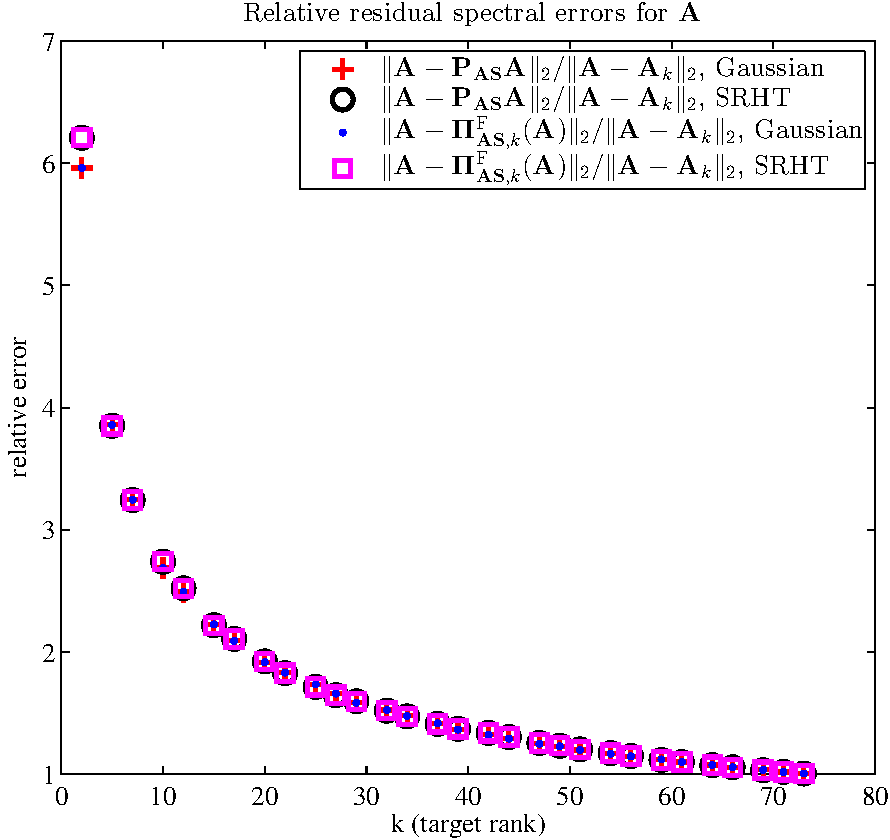
\includegraphics[width=2.8in, keepaspectratio=true]{figures/ch3/experimentA-residual-spectral.pdf}}%
 \subfigure{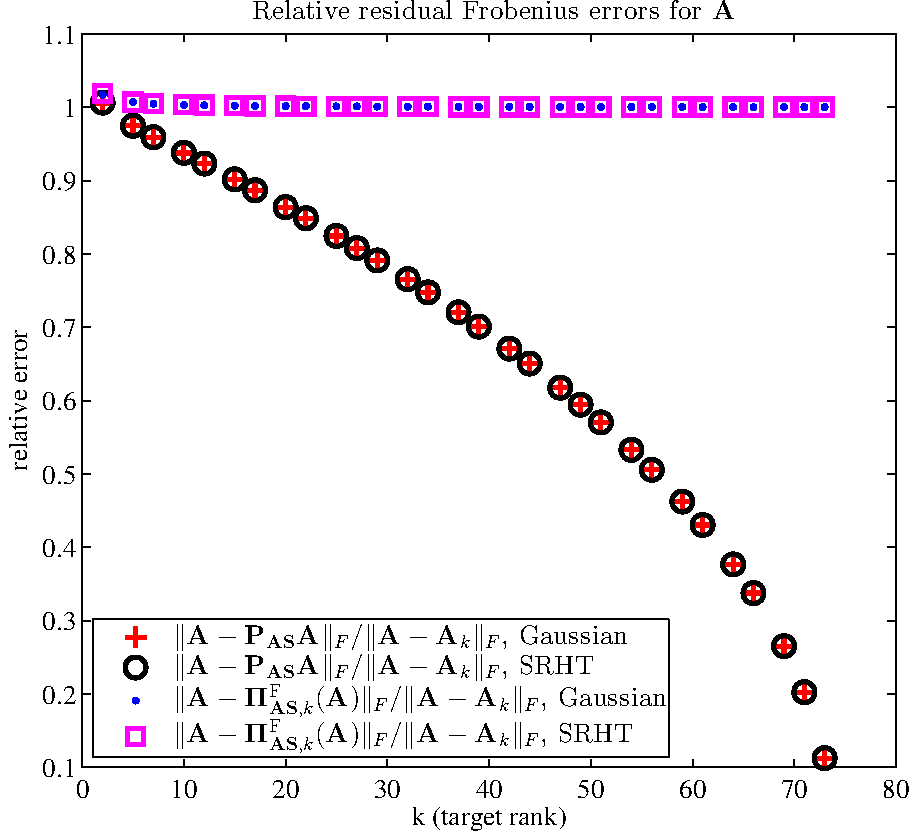
\includegraphics[width=2.8in, keepaspectratio=true]{figures/ch3/experimentA-residual-frobenius.pdf}}\\%
 \subfigure{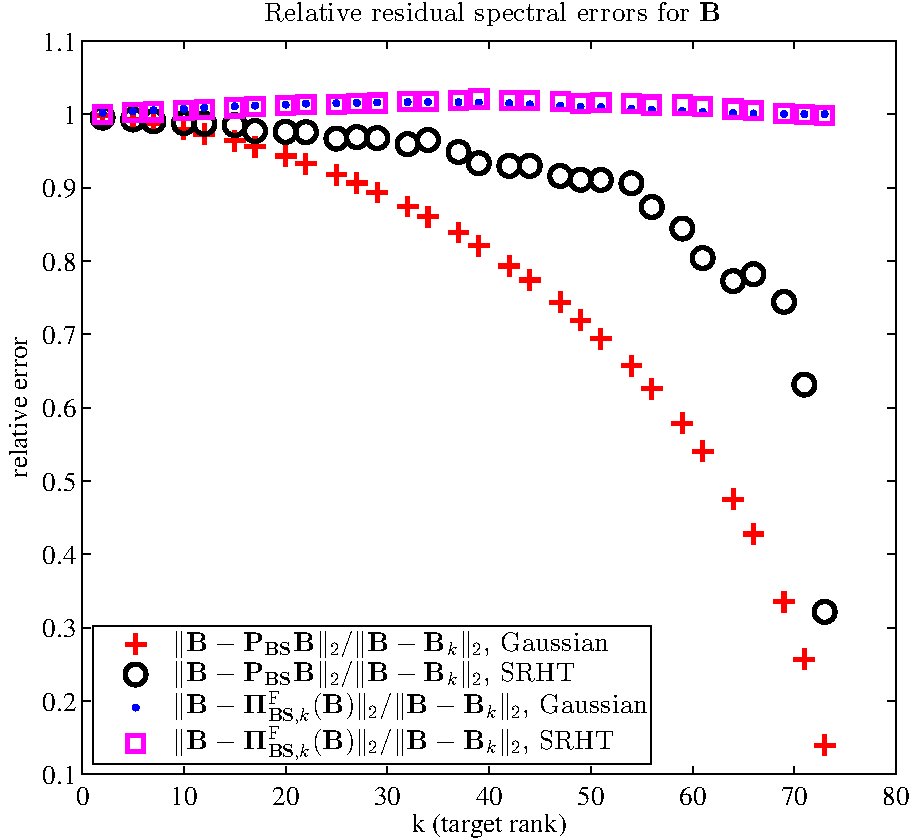
\includegraphics[width=2.8in, keepaspectratio=true]{figures/ch3/experimentB-residual-spectral.pdf}}%
 \subfigure{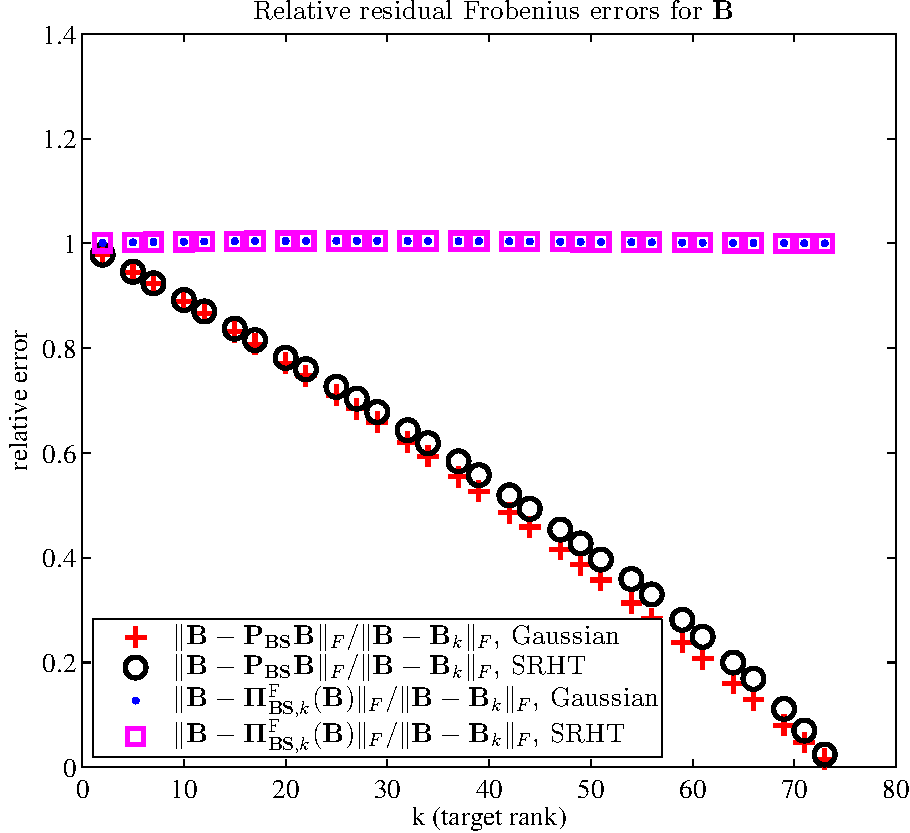
\includegraphics[width=2.8in, keepaspectratio=true]{figures/ch3/experimentB-residual-frobenius.pdf}}\\%
 \subfigure{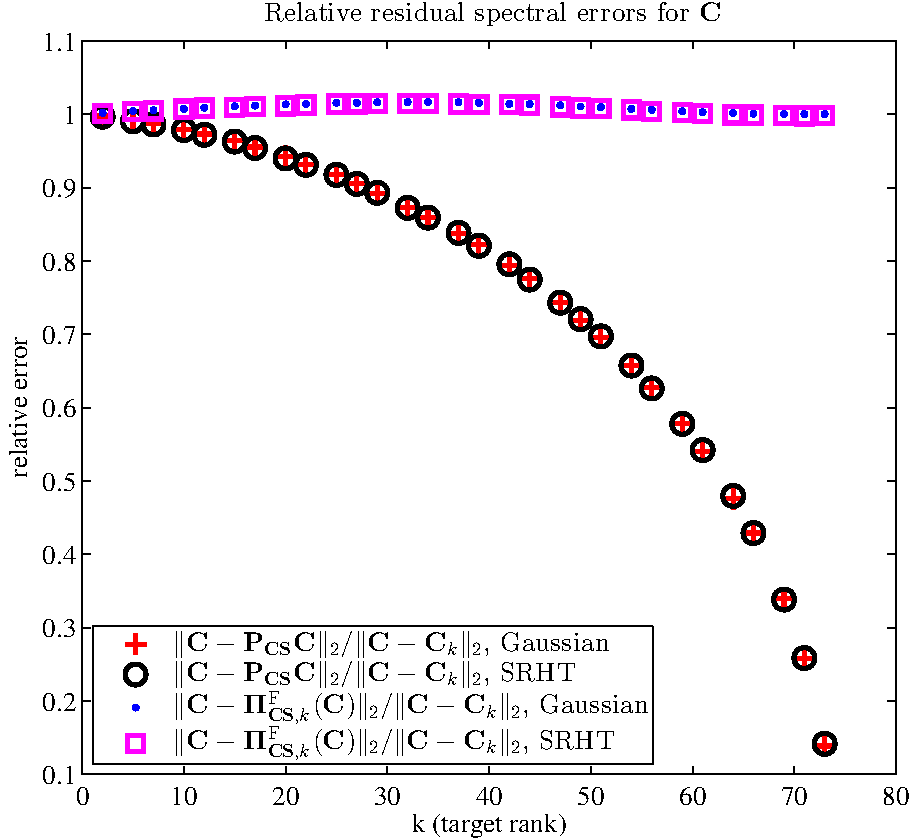
\includegraphics[width=2.8in, keepaspectratio=true]{figures/ch3/experimentC-residual-spectral.pdf}}%
 \subfigure{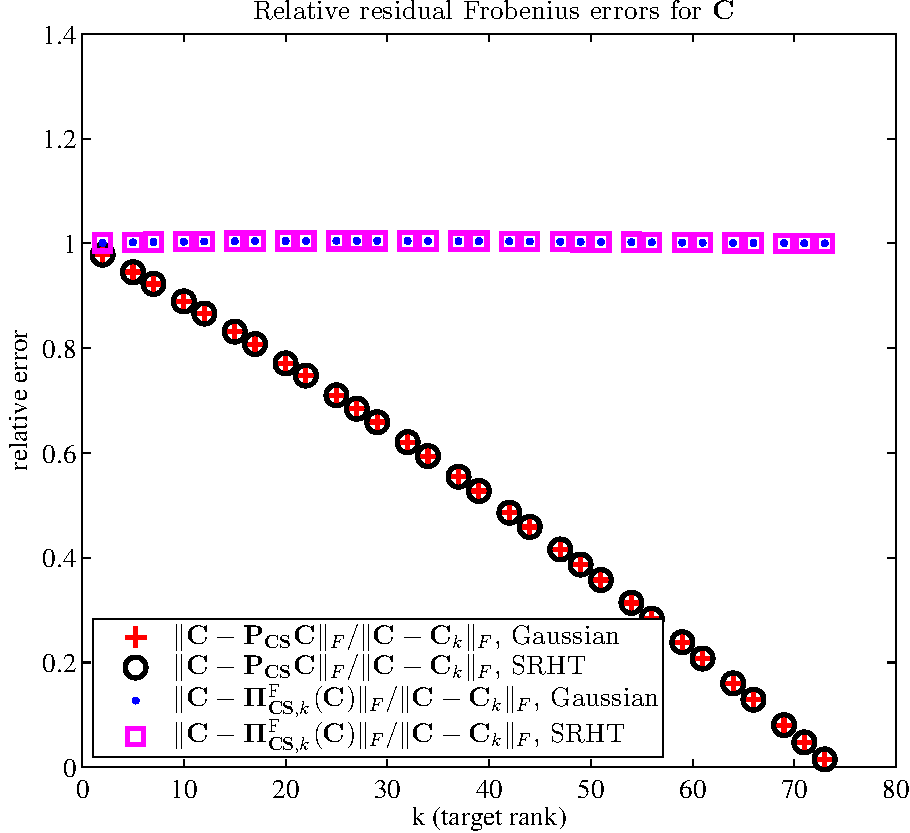
\includegraphics[width=2.8in, keepaspectratio=true]{figures/ch3/experimentC-residual-frobenius.pdf}}%
 \caption[Residual errors of low-rank approximation algorithms]{
 {\sc Residual errors of low-rank approximation algorithms.} Relative 
 spectral and Frobenius-norm residual errors of the SRHT and Gaussian low-rank approximation 
 algorithms ($\XNorm{\matM - \matP_{\matM\matS} \matM}/\XNorm{\matM - \matM_k}$ 
 and $\XNorm{\matM - \boldPi_{\matM\matS, k}^{\mathrm{F}}(\matM)}/\XNorm{\matM - \matM_k}$ 
 for $\xi = 2, \mathrm{F}$)
 as a function of the target rank $k$ for the three matrices $\matM = \matA, \matB, \matC.$ 
 Each point is the average error observed over 30 trials. 
 In each trial, $\ell = \lceil 2 k \log n \rceil$ column samples were used.}
 \label{ch3:fig:residualerrors}
\end{figure}
%
Figure~\ref{ch3:fig:residualerrors} depicts the relative residual errors of 
the Gaussian and SRHT algorithms for approximations generated using 
Algorithms~\ref{ch3:alg:nonfixedrank-randomized-svd} and~\ref{ch3:alg:fixedrank-randomized-svd}:
$\matP_{\matM\matS} \matM$ and $\boldPi_{\matM\matS, k}^{\mathrm{F}}(\matM),$ which we shall hereafter 
refer to respectively as the non-rank-restricted and rank-restricted 
approximations. Here the matrix $\matM$ is used to refer interchangeably to 
$\matA, \matB,$ and $\matC.$ The relative residual errors 
($\XNorm{\matM - \matP_{\matM\matS} \matM}/\XNorm{\matM - \matM_k}$ 
 and $\XNorm{\matM - \boldPi_{\matM\matS, k}^{\mathrm{F}}(\matM)}/\XNorm{\matM - \matM_k}$ 
 for $\xi = 2, \mathrm{F}$) shown in this figure for each value of $k$ were 
obtained by taking the average of the relative residual errors observed over 
30 trials of low-rank approximations, each formed using 
$\ell = \lceil 2 k \log n \rceil$ samples.

With the exception of the residual spectral errors on $\mat{A},$ 
which range from between two and nine times the size of the optimal rank-$k$ spectral
residual error for $k < 20,$ we see that the residual errors for all three
matrices are less than 1.1 times the residual error of $\matM_k,$ if not
significantly smaller. Specifically, the relative residual errors of the
restricted-rank approximations remain less than 1.1 over the entire range of $k$
while the relative residual errors of the non-rank-restricted approximations
actually decrease as $k$ increases.  Note that, because $\ell >k,$ the
relative errors of the non-rank-restricted approximations are often smaller
than 1, while those of the restricted-rank approximations are never smaller
than 1.

Since the matrices $\mat{B}$ and $\matC$ have the same singular values, but the
singular spaces of $\matC$ are less coherent, the difference in the residual errors of
the approximations of $\mat{B}$ and $\mat{C}$ is evidence that
the spectral-norm accuracy of the SRHT approximations is increased on less
coherent datasets; the same is true for the Frobenius norm accuracy to a lesser
extent. The Gaussian approximations seem insensitive to the level of coherence.
Only on the highly coherent matrix $\mat{B}$ do we see a notable decrease in
the residual errors when Gaussian sampling is used rather than an SRHT; however,
even in this case the residual errors of the SRHT approximations are comparable
with that of $\matB_k.$ In all, Figure~\ref{ch3:fig:residualerrors} suggests
that the gain in computational efficiency provided by the SRHT does not come at
the cost of a significant loss in accuracy and that taking $\ell = \lceil 2 k \log n
\rceil$ samples suffices to obtain approximations with small residual errors
relative to those of the optimal rank-$k$ approximations. Up to the 
specific
value of the constant, this latter observation coincides with the conclusions of
Theorems~\ref{ch3:thm:quality-of-approximation-guarantee-spectral} 
and~\ref{ch3:thm:quality-of-approximation-guarantee-Frobenius}.

\begin{figure}[htp]
 \subfigure{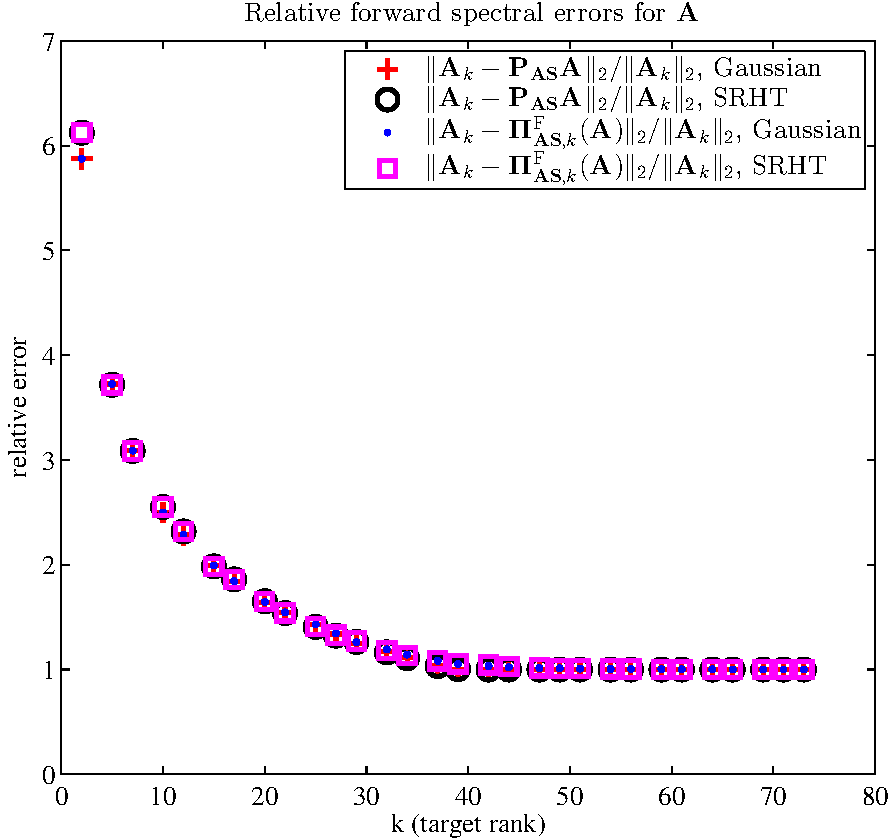
\includegraphics[width=2.8in, keepaspectratio=true]{figures/ch3/experimentA-forward-spectral.pdf}}%
 \subfigure{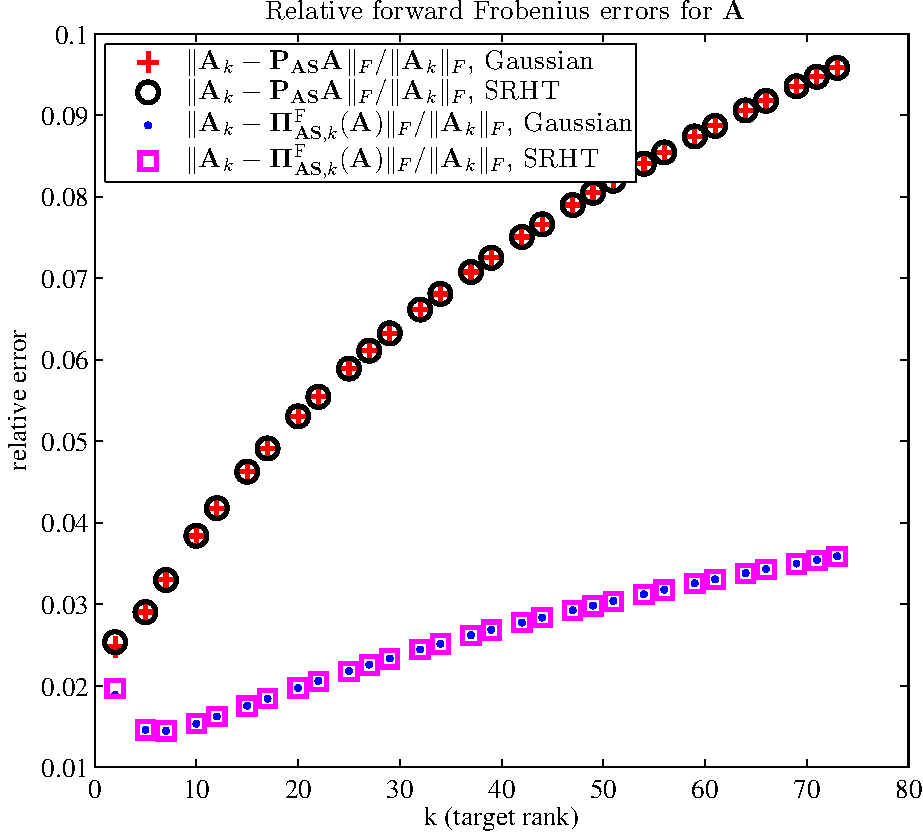
\includegraphics[width=2.8in, keepaspectratio=true]{figures/ch3/experimentA-forward-frobenius.pdf}}\\%
 \subfigure{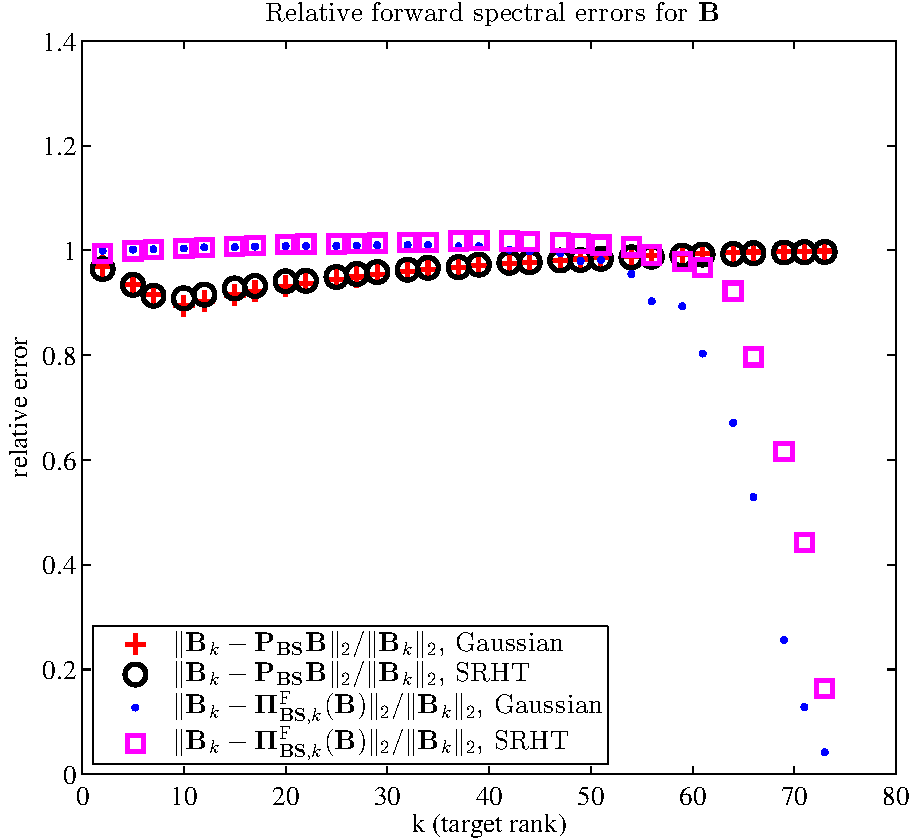
\includegraphics[width=2.8in, keepaspectratio=true]{figures/ch3/experimentB-forward-spectral.pdf}}%
 \subfigure{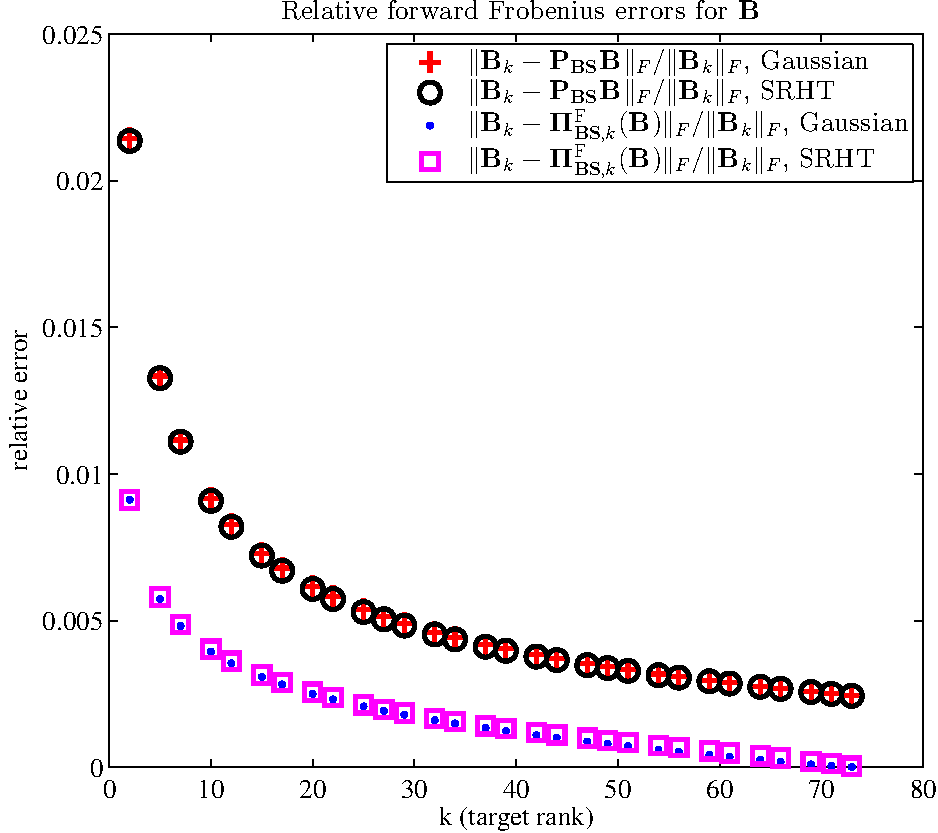
\includegraphics[width=2.8in, keepaspectratio=true]{figures/ch3/experimentB-forward-frobenius.pdf}}\\%
 \subfigure{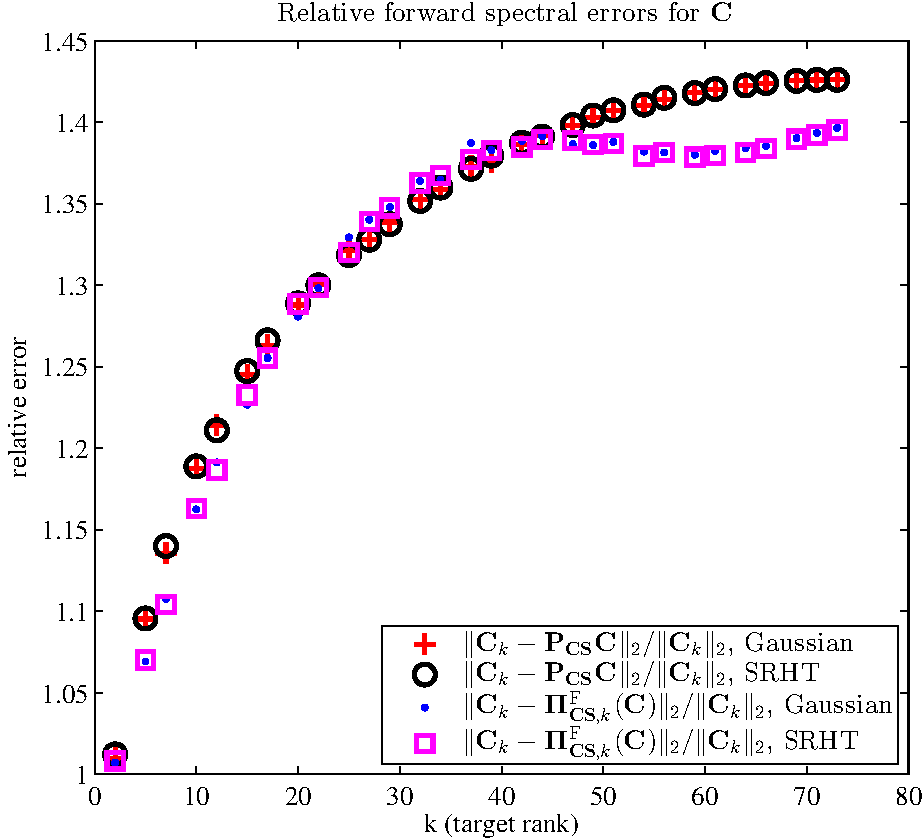
\includegraphics[width=2.8in, keepaspectratio=true]{figures/ch3/experimentC-forward-spectral.pdf}}%
 \subfigure{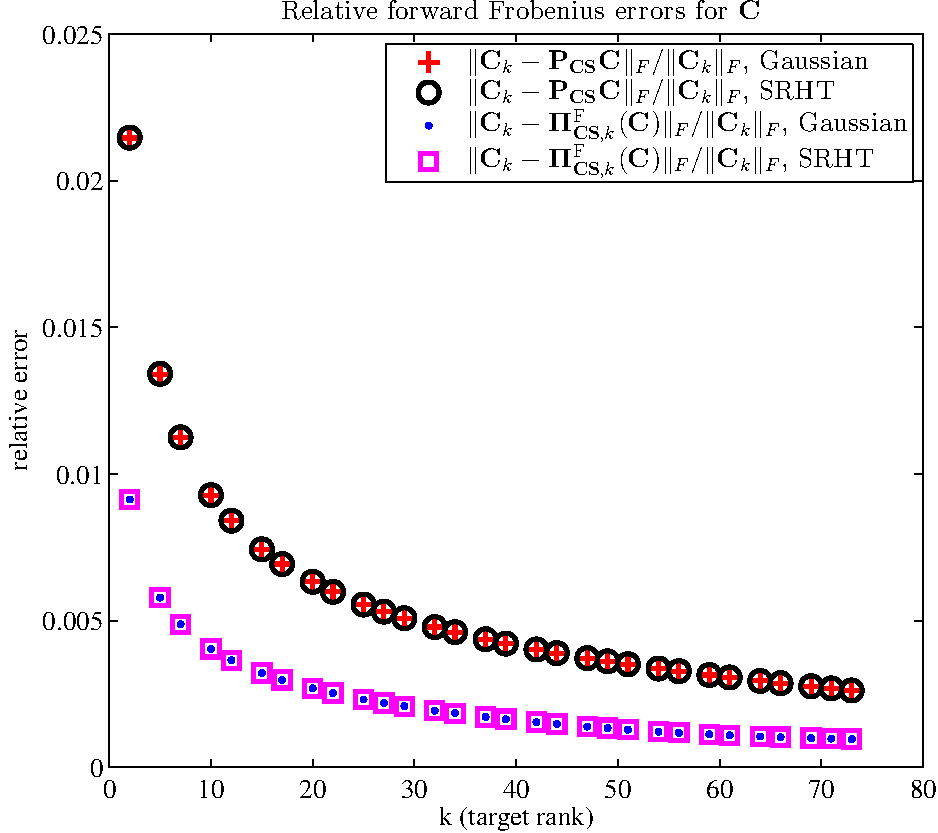
\includegraphics[width=2.8in, keepaspectratio=true]{figures/ch3/experimentC-forward-frobenius.pdf}}%
 \caption[Forward errors of low-rank approximation algorithms]{
 {\sc Forward errors of low-rank approximation algorithms.} The 
 relative spectral and Frobenius-norm forward errors of the SRHT and Gaussian low-rank approximation algorithms
 ($\XNorm{\matM_k - \matP_{\matM\matS} \matM}/\XNorm{\matM - \matM_k}$ 
 and $\XNorm{\matM_k - \boldPi_{\matM\matS, k}^{\mathrm{F}}(\matM)}/\XNorm{\matM - \matM_k}$ 
 for $\xi = 2, \mathrm{F}$)
 as a function of the target rank $k$ for the three matrices $\matM = \matA, \matB, \matC.$ Each point is the average of the errors observed over 30 trials.
 In each trial, $\ell = \lceil 2 k \log n \rceil$ column samples were used.}
 \label{ch3:fig:forwarderrors}
\end{figure}

Figure~\ref{ch3:fig:forwarderrors} depicts the relative forward errors of the
Gaussian and SRHT algorithms ($\XNorm{\matM_k - \matP_{\matM\matS} \matM}/\XNorm{\matM - \matM_k}$ 
 and $\XNorm{\matM_k - \boldPi_{\matM\matS, k}^{\mathrm{F}}(\matM)}/\XNorm{\matM - \matM_k}$ 
 for $\xi = 2, \mathrm{F}$) for the
non-rank-restricted and rank-restricted approximations. The error shown for each
$k$ is the average relative forward error observed over 30 trials of low-rank
approximations each formed using $\ell = \lceil 2 k \log n\rceil$ samples. We
observe that the forward errors of both algorithms for both choices of sampling
matrices are on the scale of the norm of $\mat{M}_k.$ By looking at the relative
spectral-norm forward errors we see that in this norm, perhaps contrary to
intuition, the rank-restricted approximation does not provide a more accurate
approximation to $\matM_k$ than does the non-rank-restricted approximation.
However the rank-restricted approximation clearly provides a more accurate
approximation to $\matM_k$ than the non-rank-restricted 
approximation in the
Frobenius norm. A rather
unexpected observation is that the rank-restricted approximations are more
accurate in the spectral norm for highly coherent matrices ($\matB$) than they
are for matrices which are almost minimally coherent ($\matC$). Overall,
Figure~\ref{ch3:fig:forwarderrors} suggests that the SRHT low-rank approximation
algorithms provide accurate approximations to $\matM_k$ when $\ell$ is in the
regime suggested by Theorems~\ref{ch3:thm:quality-of-approximation-guarantee-spectral}
and~\ref{ch3:thm:quality-of-approximation-guarantee-Frobenius}.

\begin{figure}
 \centering
 \subfigure{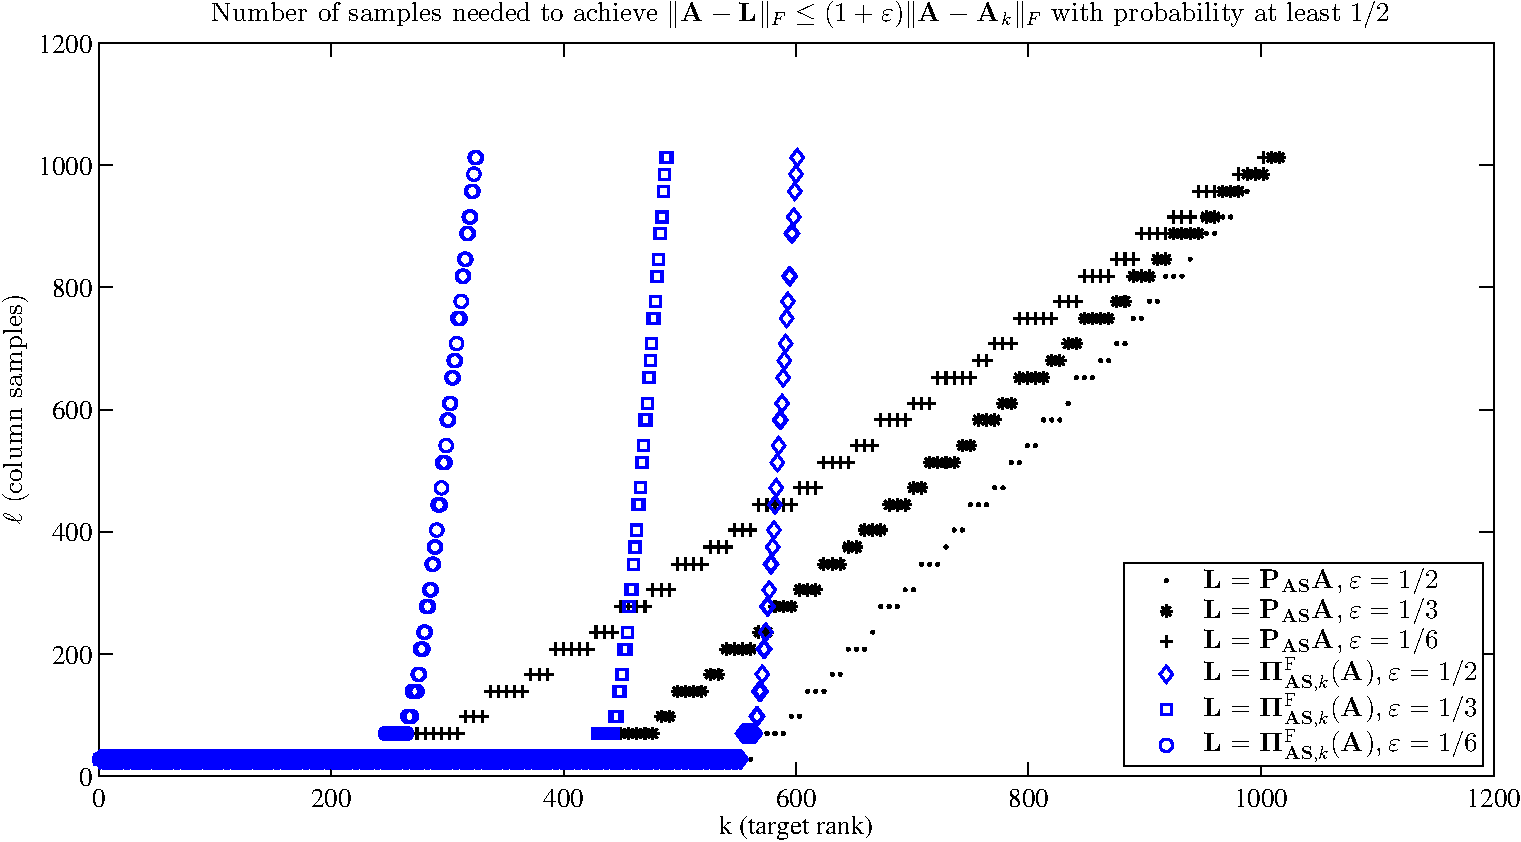
\includegraphics[width=4.9in, keepaspectratio=true]{figures/ch3/experimentA-empirically-necessary-r.pdf}}\\%
 \subfigure{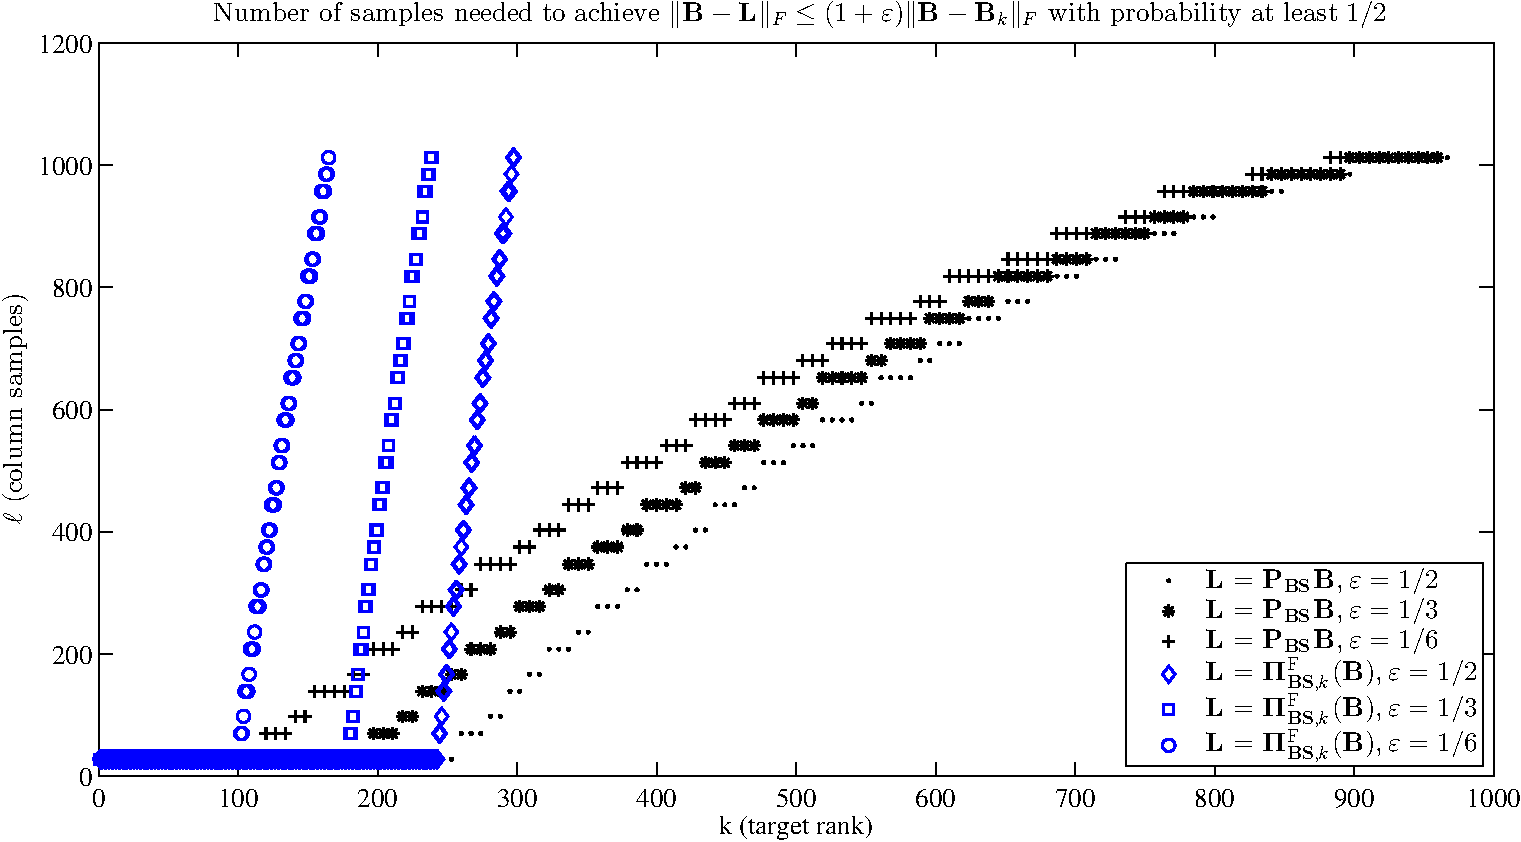
\includegraphics[width=4.9in, keepaspectratio=true]{figures/ch3/experimentB-empirically-necessary-r.pdf}}\\%
 \subfigure{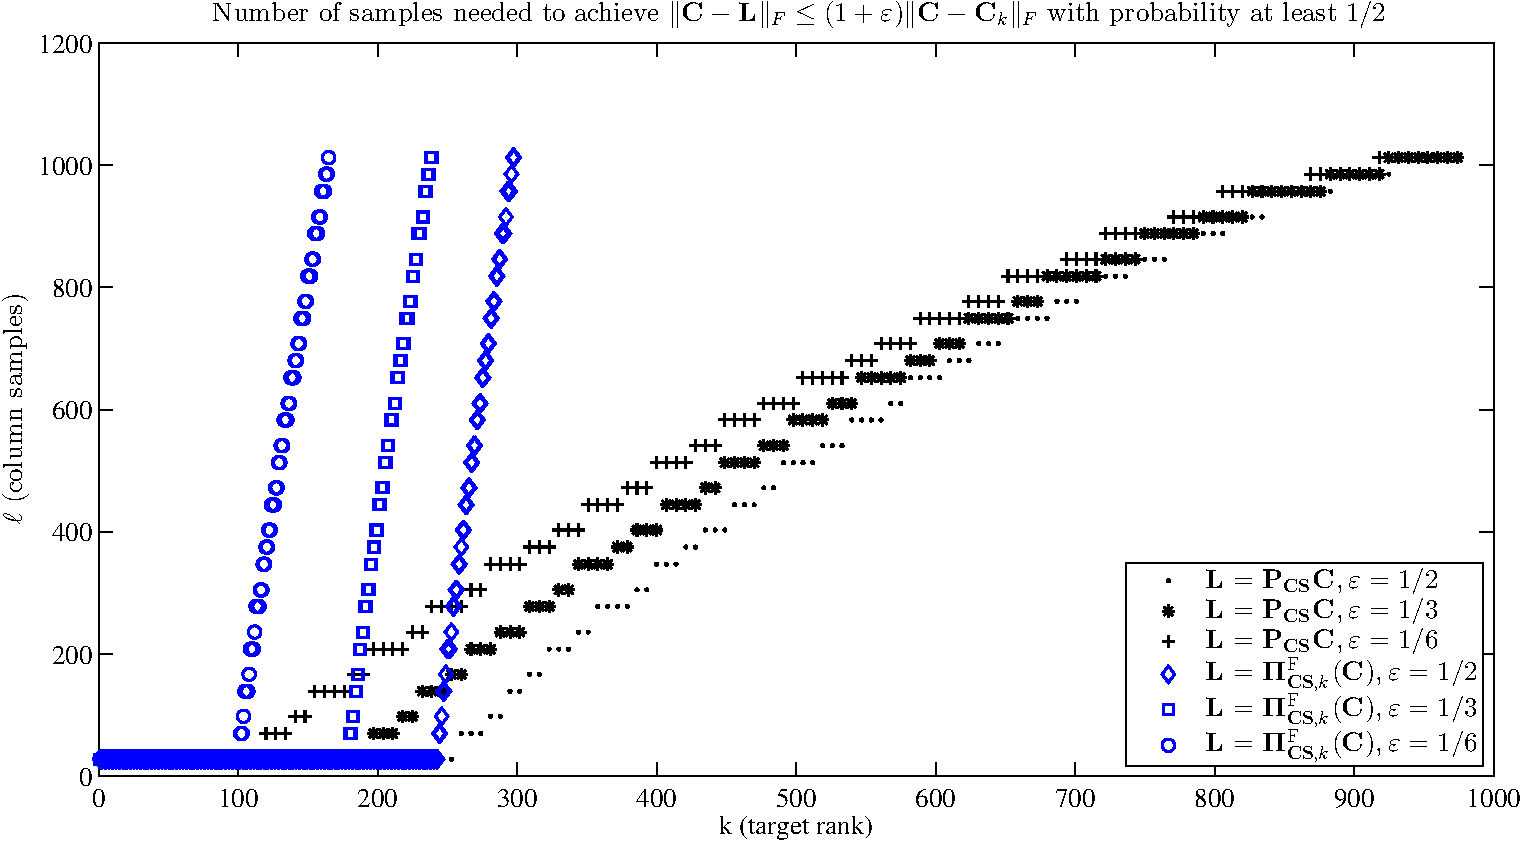
\includegraphics[width=4.9in, keepaspectratio=true]{figures/ch3/experimentC-empirically-necessary-r.pdf}}
 \caption[The number of column samples required for relative error Frobenius-norm approximations]{
 {\sc The number of column samples required for relative error Frobenius-norm approximations.} The 
 value of $\ell$ empirically necessary to ensure that, with probability at least one-half, approximations generated
 by the SRHT algorithms satisfy $\FNorm{\matM - \matP_{\matM\matTh\transp} \matM} \leq (1 + \epsilon) \FNorm{\matM - \matM_k}$ and 
 $\FNorm{\matM - \boldPi_{\matM\matTh\transp, k}^{\mathrm{F}}(\matM)} \leq (1 + \epsilon) \FNorm{\matM - \matM_k}$ (for $\matM = \matA, \matB, \matC$).}
 \label{ch3:fig:empiricalrnecessary}
\end{figure}

\subsection{Empirical evaluation of our error bounds}
Figures~\ref{ch3:fig:residualerrors} and~\ref{ch3:fig:forwarderrors} show that when 
$\ell = \lceil 2 k \log n \rceil$ samples are taken, the SRHT low-rank approximation algorithms 
both provide approximations to $\matM$ that are within a factor of $1 + \epsilon$ as 
accurate in the Frobenius norm as $\matM_k,$ as Theorem~\ref{ch3:thm:quality-of-approximation-guarantee-Frobenius} 
suggests should be the case. More precisely, Theorem~\ref{ch3:thm:quality-of-approximation-guarantee-Frobenius} 
assures us that $528 \epsilon^{-1} [\sqrt{k} + \sqrt{8 \log(8 n/\delta)}]^2 \log(8k/\delta)$ column 
samples are sufficient to ensure that, with at least probability $1 - \delta$, $\matP_{\matM \matTh\transp} \matM$ 
and $\boldPi_{\matM\matTh\transp, k}^{\mathrm{F}}(\matM)$ have Frobenius norm residual and forward error 
within $1 + \epsilon$ 
of that of $\matM_k.$ The factor $528$ can certainly be reduced by optimizing the numerical 
constants given in Theorem~\ref{ch3:thm:quality-of-approximation-guarantee-Frobenius}. 
But what is the smallest $\ell$ that ensures the
Frobenius norm residual error bounds 
$\FNorm{\matM - \matP_{\matM\matTh\transp} \matM} \leq (1 + \epsilon) \FNorm{\matM - \matM_k}$ and 
 $\FNorm{\matM - \boldPi_{\matM\matTh\transp, k}^{\mathrm{F}}(\matM)} \leq (1 + \epsilon) \FNorm{\matM - \matM_k}$ are 
satisfied with some fixed probability? To investigate, in Figure~\ref{ch3:fig:empiricalrnecessary} 
we plot the values of $\ell$ determined empirically to be sufficient to obtain $(1+\epsilon)$ 
Frobenius norm residual errors relative to the optimal rank-$k$ approximation; we fix the 
failure probability $\delta=1/2$ and vary $\epsilon.$ Specifically, the $\ell$ plotted for
each $k$ is the smallest number of samples for which 
$\FNorm{\matM - \matP_{\matM\matTh\transp} \matM} \leq (1 + \epsilon) \FNorm{\matM - \matM_k}$ 
or $\FNorm{\matM - \boldPi_{\matM\matTh\transp, k}^{\mathrm{F}}(\matM)} \leq (1 + \epsilon) \FNorm{\matM - \matM_k}$
in at least 15 out of 30 trials.

It is clear that, for fixed $k$ and $\epsilon,$ the number of samples $\ell$ required 
to form a non-rank-restricted approximation to $\matM$ with $1+\epsilon$ relative 
residual error is smaller than the $\ell$ required to form a rank-restricted approximation 
with $1+\epsilon$ relative residual error. Note that for small values of $k$, the 
$\ell$ necessary for relative residual error to be achieved is actually smaller than $k$ for 
all three datasets. This is a reflection of the fact that when $k_1 < k_2$ are small, the 
ratio $\FNorm{\matM - \matM_{k_2}}/\FNorm{\matM - \matM_{k_1}}$ is very close to one. Outside 
of the initial flat regions, the empirically determined value of $r$ seems to grow linearly with $k$;
this matches with the observation of Woolfe et al. that taking $\ell=k+8$ suffices to 
consistently form accurate low-rank approximations using the SRFT scheme, which is 
very similar to the SRHT scheme~\cite{WLRT08}. We also note that this matches with 
Theorem~\ref{ch3:thm:quality-of-approximation-guarantee-Frobenius}, which predicts that the 
necessary $\ell$ grows at most linearly with $k$ with a slope like $\log n.$

Finally, Theorem~\ref{ch3:thm:quality-of-approximation-guarantee-spectral} does \emph{not} guarantee 
that $1+\epsilon$ spectral-norm relative residual errors can be achieved. Instead, it 
provides bounds on the spectral-norm residual errors achieved in terms of 
$\TNorm{\matM - \matM_k}$ and $\FNorm{\matM - \matM_k}$ that are guaranteed to hold when 
$\ell$ is sufficiently large. In Figure~\ref{ch3:fig:predictedspecerrvsactual} we compare the 
spectral-norm residual error guarantees of Theorem~\ref{ch3:thm:quality-of-approximation-guarantee-spectral} 
to what is achieved in practice. To do so, we take the optimistic viewpoint that the constants 
in Theorem~\ref{ch3:thm:quality-of-approximation-guarantee-spectral} can be optimized to unity. Under 
this view, if more columns than $\ell_2 = \epsilon^{-1} [\sqrt{k} + \sqrt{\log(n/\delta)}]^2 \log(k/\delta)$ 
are used to construct the SRHT approximations, then the spectral-norm residual error is no larger than
\[
 b_2 = \left(1 + \sqrt{\frac{\log(n/\delta) \log(\rho/\delta)}{\ell}}\right) \cdot 
 \TNorm{\matM - \matM_k} + \sqrt{\frac{\log(\rho/\delta)}{\ell}} \cdot \FNorm{\matM - \matM_k},
\]
where $\rho$ is the rank of $\matM,$ with probability greater than $1-\delta.$ Our comparison consists of 
using $\ell_2$ samples to construct the SRHT approximations and then comparing the predicted upper bound on 
the spectral-norm residual error, $b_2$, to the empirically observed spectral-norm residual errors. 
Figure~\ref{ch3:fig:predictedspecerrvsactual} shows, for several values of $k$, the upper bound $b_2$ and 
the observed relative spectral-norm residual errors, with precision parameter $\epsilon = 1/2$ and 
failure parameter $\delta = 1/2.$ For each value of $k,$ the empirical spectral-norm residual error plotted 
is the average of the errors over 30 trials of low-rank approximations. Note from 
Figure~\ref{ch3:fig:predictedspecerrvsactual} that with this choice of $\ell,$ the spectral-norm residual errors 
of the rank-restricted and non-rank-restricted SRHT approximations are essentially the same.

\begin{figure}
 \centering
 \subfigure{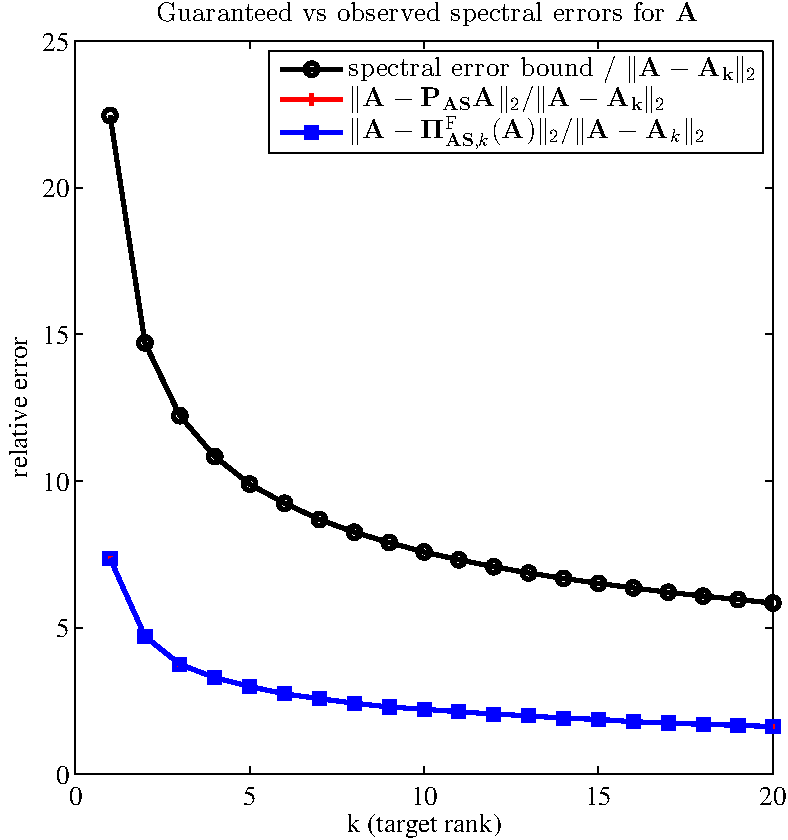
\includegraphics[width=2in, keepaspectratio=true]{figures/ch3/experimentA-actual-versus-predicted-spectral-error}}%
 \subfigure{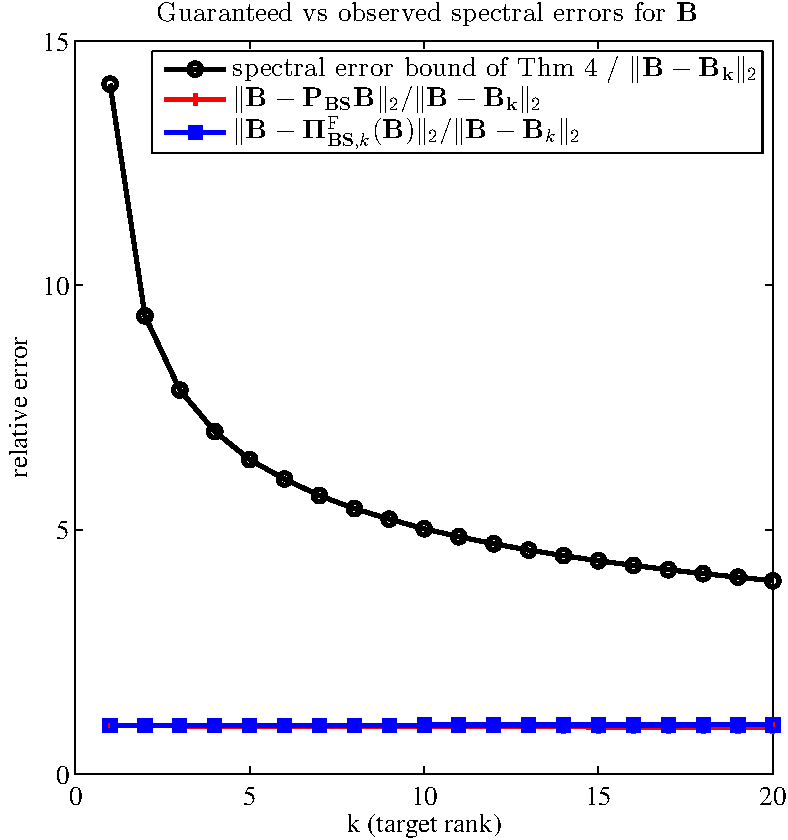
\includegraphics[width=2in, keepaspectratio=true]{figures/ch3/experimentB-actual-versus-predicted-spectral-error}}%
 \subfigure{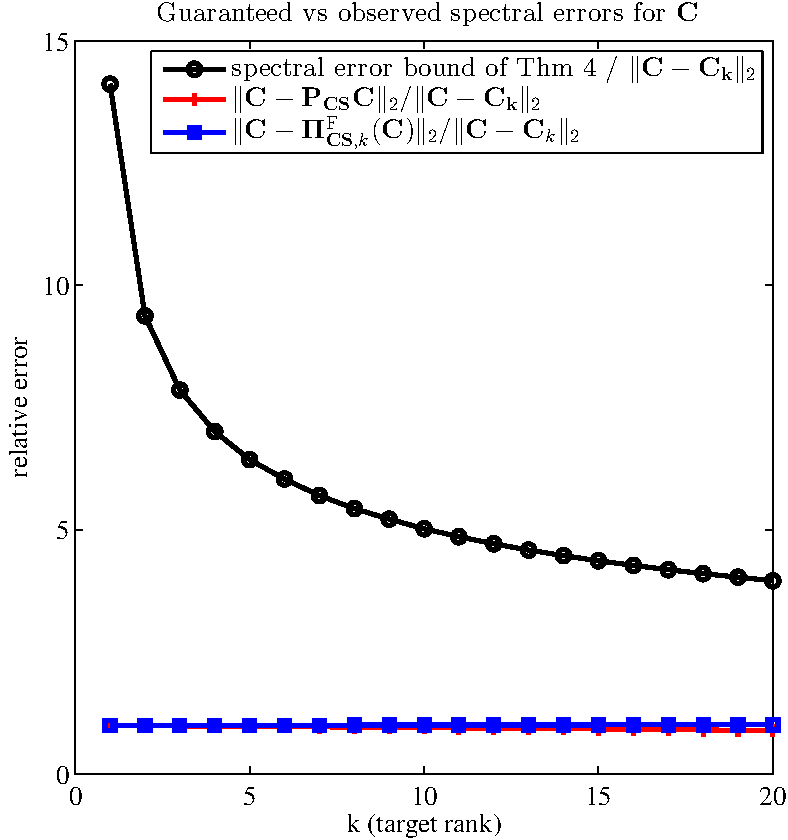
\includegraphics[width=2in, keepaspectratio=true]{figures/ch3/experimentC-actual-versus-predicted-spectral-error}}
 \caption[Empirical versus predicted spectral-norm residual errors of low-rank approximations]{%
 {\sc Empirical versus predicted spectral-norm residual errors of low-rank approximations.} The empirical spectral-norm residual errors relative to those of the optimal rank-$k$ approximants 
 ($\TNorm{\matM - \matP_{\matM\matTh\transp} \matM}/\|\matM - \matM_k\|_2$ and 
 $\|\matM - \boldPi_{\matM\matTh\transp,k}^{\mathrm{F}}(\matM)\|_2/\|\matM - \matM_k\|_2$) plotted alongside the same ratio for the bounds given in 
 Theorem~\ref{ch3:thm:quality-of-approximation-guarantee-spectral}, when $\ell = \lceil 2[\sqrt{k} + \sqrt{\log(2n)}]^2 \log(2k) \rceil$ 
 (for $\matM = \matA, \matB, \matC$). On the scale shown, the errors of the two SRHT-based approximation algorithms are essentially identical.}
 \label{ch3:fig:predictedspecerrvsactual}
\end{figure}

Judging from Figures~\ref{ch3:fig:empiricalrnecessary} and~\ref{ch3:fig:predictedspecerrvsactual}, even when we
assume the constants present can be optimized away, the bounds given in Theorems~\ref{ch3:thm:quality-of-approximation-guarantee-spectral}
and~\ref{ch3:thm:quality-of-approximation-guarantee-Frobenius}
are pessimistic: it seems that in fact approximations with Frobenius-norm residual error within $1+\epsilon$ of the error of the
optimal rank-$k$ approximation can be obtained with $\ell$ linear in $k,$ and the spectral-norm residual errors are smaller than the supplied upper bounds.
Thus there is still room for improvement in our understanding of the SRHT low-rank approximation algorithm, but as explained in Section~\ref{ch3:sec:priorwork},
ignoring constants, the bounds of Theorem~\ref{ch3:thm:quality-of-approximation-guarantee-spectral} are often tighter than those obtained in earlier works.

To bring perspective to this discussion, consider that even if one limits consideration to deterministic algorithms, the
known error bounds for the Gu--Eisenstat rank-revealing QR---a popular and widely used algorithm for low-rank 
approximation---are quite pessimistic and do not reflect the excellent accuracy that is seen in practice~\cite{GE96}. 
Regardless, we do not advocate using these approximation schemes for applications in which highly accurate low-rank 
approximations are needed. Rather, Theorems~\ref{ch3:thm:quality-of-approximation-guarantee-spectral} 
and~\ref{ch3:thm:quality-of-approximation-guarantee-Frobenius} and our numerical experiments 
suggest that they are appropriate in situations where one is willing to trade some accuracy for a gain in computational efficiency.

%!TEX root = thesis.tex

\chapter{Theoretical and empirical aspects of SPSD sketches}
\label{ch4}

\todo[inline]{See how good is the spectral norm bound obtained using an M*-estimate argument using RV's coordinate projection result}
\todo[inline]{Include the spectral norm bound obtained using concentration on the symmetric group}
\todo[inline]{Add the large-scale analysis using CD's perturbation result}
\todo[inline]{Fix the remarks throughout thesis so environment is consistent}

\section{Introduction}

In this chapter we consider the accuracy of randomized low-rank approximations of symmetric 
positive-semidefinite matrices conforming to the following general model\footnote{The content of this chapter is redacted from
the technical report~\cite{Git12} and the technical report~\cite{GM13} coauthored with Michael Mahoney. A preliminary version of some of these results appear in
the conference paper~\cite{GM13_ICML}, also coauthored with Michael Mahoney.}.
%

\paragraph{SPSD Sketching Model.}
Let $\matA$ be an $n \times n$ SPSD matrix, and 
let $\matS$ be matrix of size $n \times \ell$, where $\ell \ll n$. 
Form
\[
 \matC = \matA \matS \quad \text{ and } \quad \matW = \matS\transp \matA \matS.
\]
%and take $\matC \matW^\pinv \matC\transp$ to be the low-rank approximation to $\matA.$
We call $\matC \matW^\pinv \matC\transp$ the \emph{SPSD sketch} of $\matA$ associated with the
\emph{sketching matrix} $\matS.$ Note that this sketch is also SPSD, and has rank
at most $\ell.$

\paragraph{} These sketches can be computed quickly, and as we see in Section~\ref{ch4:sxn:emp},
are accurate low-rank approximations for several classes of matrices that arise in machine learning
and data analysis applications. This model subsumes
both projection-based sketches (here, $\matS$ mixes the columns and rows of $\matA$),
and sampling-based sketches (here, $\matS$ selects columns and rows of $\matA$).

The computation of an SPSD sketch requires only one pass over $\matA,$ because
the matrix $\matC = \matA\matS$ uniquely determines the sketch. One should contrast this
to the natural extension of the low-rank approximations considered in Chapter~\ref{ch3},
namely $\matP_{\matA\matS} \matA \matP_{\matA\matS},$ which requires two passes over
$\matA$ : one to construct a basis for the range of $\matA\matS,$ and one to project
$\matA$ onto this basis. 

In addition to one-pass sketches, low-rank approximations formed using the so-called power method~\cite{HMT11}
fit the SPSD sketching model.
For such sketches, $\matC = \matA^q \matS_0$ and $\matW = \matS_0\transp \matA^{2q-1} \matS_0$ for some
integer $q \geq 2$ and sketching matrix $\matS_0$. To see that these models fit the SPSD sketching model,
simply consider the sketching matrix to be $\matS = \matA^{q-1} \matS_0.$ The approximation errors of these
sketches decrease as $p$ increases. The two-pass sketch is particularly of interest: we relate it to a 
low-rank approximation proposed in~\cite{HMT11}. 
As well, we show empirically that two-pass SPSD sketches are empirically significantly more accurate than the 
projection-based low-rank approximant $\matP_{\matA \matS} \matA \matP_{\matA \matS}.$

When $\matS$ comprises columns selected uniformly
at random without replacement from the $n \times n$ identity matrix, the resulting SPSD 
sketch is called a Nystr\"om extension. To form a Nystr\"om extension, 
one needs only to be able to sample columns from $\matA.$ Further, the cost of 
forming the factored form of a Nystr\"om extension is $\Omega(\ell^3 + n\ell),$
linear in the size of $\matA$! For these two reasons, Nystr\"om extensions are attractive in settings where it is
costly or unreasonable to access all the elements of $\matA.$
However, as we see in this chapter, the use of Nystr\"om
extensions is only theoretically justified when the top $k$-dimensional eigenspace of $\matA$ has
low coherence. Recall from Chapter~\ref{chprelim} that the coherence of this eigenspace is defined as
\[
 \mu = \max_{i=1,\ldots,n} \frac{n}{k} \big\|(\matP_{\matU_1})_{ii} \big\|_2^2,
\]
where $\matU_1$ is a basis for the eigenspace.
This dependence on the coherence is not simply a theoretical consideration:
it is empirically observable. This motivates looking at the wider class of SPSD sketches, where, depending on the choice of $\matS$, 
potentially \emph{all} the columns of the matrix contribute to the approximation. 

This
chapter presents theoretical and empirical results for different choices of $\matS.$
Empirically, we find that the Nystr\"om extension performs well in practice, but
not as well as sketches that mix the columns of $\matA$ before sampling or sketches
that sample the columns according to a specific importance sampling distribution.
Our theoretical bounds bear out this comparison, and are asymptotically superior
to the bounds present in the literature for low-rank approximation schemes
which fit into our SPSD sketching model. However, a large gap still remains between
our bounds and the observed errors of SPSD sketches.

We develop a framework for the analysis of SPSD sketches that parallels the framework 
Lemma~\ref{chprelim:lem:structural-result} provides for the analysis of projection-based
low-rank approximations. Applied to Nystr\"om extensions, our framework exposes a natural connection between Nystr\"om extensions 
and the column subset selection problem that leads to an optimal worse-case bound for
the spectral error of Nystr\"om extensions. This is the first truly
relative-error spectral norm bound available for Nystr\"om extensions; 
the contemporaneous work~\cite{CD11} independently establishes this same bound in the
broader context of CUR decompositions. More generally, we provide
theoretical worst-case bounds for several sketches based on random column sampling and random projections.
These bounds apply to both
one-pass and multiple-pass sketches. In the case of multiple-pass sketches, we find that
the errors of the sketches decrease proportionally to $\lambda_{k+1}(\matA)/\lambda_k(\matA)$
with each additional pass.

In general, the process of computing SPSD sketches is not numerically stable: if $\matW$ is 
ill-conditioned, then instabilities may arise in solving the linear system 
$\matW^\dagger \matC\transp$. 
This is of particular concern with Nystr\"om extensions, since the particular
submatrix of $\matA$ selected may be quite ill-conditioned. With other sketching schemes,
the fact that $\matW$ is formed as a mixture of the columns of $\matA$ tends to
provide implicit protection against $\matW$ being poorly conditioned. The seminal
paper on the use of Nystr\"om extensions for low-rank approximation,~\cite{WS01},
suggested regularizing Nystr\"om extensions to avoid ill-conditioning. This
algorithm can be used to regularize the computation of any SPSD sketch; we provide
the first error bounds for these regularized sketches. Another regularization
scheme is introduced in~\cite{CD11}. We compare the empirical performance of these
two regularization schemes.

We supplement our theoretical results with a collection of empirical results intended
to illustrate the performance of the considered SPSD sketches on matrices that
arise in machine learning applications. We also provide empirical results for the
rank-restricted sketches obtained by replacing $\matW$ with $\matW_k$ in the 
definition of an SPSD sketch. That is, we also consider sketches of the form
$\matC \matW_k^\pinv \matC\transp.$ These sketches do not fit into our SPSD
sketching model, but are the natural way to ensure that the rank of the low-rank
approximation does not exceed the target rank $k.$ Further, since $\matW_k$ has
a smaller condition number than $\matW,$ the rank-restricted sketches can be
computed more stably than the non-rank-restricted sketches.

%

\subsection{Outline} In Section~\ref{ch4:sec:results}, we introduce the specific
randomized SPSD sketches analyzed in this chapter and summarize the
spectral, Frobenius, and trace-norm error bounds for the one-pass variants of these sketches.
In Section~\ref{ch4:sec:priorwork}, we compare our
results with prior work on SPSD sketches, in particular Nystr\"om extensions. 
In Section~\ref{ch4:sec:structuralresults} we
prove the deterministic error bounds that form the basis of our analyses. In 
Sections~\ref{ch4:sec:nystromextensions} and~\ref{ch4:sec:mixturesketches} 
we apply the deterministic bounds to the Nystr\"om extension and several randomized
mixture-based sketches. In Section~\ref{ch4:sec:stablealgs}, we recall two algorithms
for computing regularized SPSD sketches; a novel error analysis is presented for
one of these algorithms. In Section~\ref{ch4:sec:experiments} we provide
experimental evidence of the efficacy of the two algorithms for computing
regularized SPSD sketches. We provide a set of empirical results on the 
application of SPSD sketches to matrices drawn from
data analysis and machine-learning applications in Section~\ref{ch4:sxn:emp}. Finally,
we conclude in Section~\ref{ch4:sec:comparison} with an empirical comparison
of two-pass SPSD sketches with the low-rank approximation $\matP_{\matA \matS} \matA \matP_{\matA \matS}.$
In the same section, we show that a certain low-rank approximation introduced in~\cite{HMT11}
is in fact a two-pass SPSD sketch.


\section{Deterministic bounds on the errors of SPSD sketches}
\label{ch4:sec:results}
Recall the following partitioning of the eigenvalue decomposition of $\mat{A}$, 
which we use to state our results:
\begin{equation}
\mat{A} = \bordermatrix[{[}{]}]{%
&^k \vspace{-0.75ex} & \!\!^{n-k}  \hspace{1ex}\\
& \vspace{0.25ex} \mat{U}_1 \hspace{-2ex} & \mat{U}_2 
}
\bordermatrix[{[}{]}]{%
& \vspace{-0.75ex} ^k &\!\!^{n-k} \hspace{1ex}\\
& \mat{\Sigma}_1 & \\
& \vspace{0.5ex} & \mat{\Sigma}_2 
}
\bordermatrix*[{[}{]}]{%
\mat{U}_1\transp \!\! & \\
\vspace{-1ex} \mat{U}_2\transp \!\! & \\
 \vspace{-1ex} &
}.
\label{ch4:eqn:svdpartition}
\end{equation}

The matrix $[\mat{U}_1\  \mat{U}_2]$ is orthogonal, $\mat{\Sigma}_1$ contains
the $k$ largest eigenvalues of $\mat{A},$ and the columns of $\mat{U}_1$ and
$\mat{U}_2$ respectively span a top $k$-dimensional eigenspace of
$\mat{A}$ and the corresponding bottom $(n-k)$-dimensional eigenspace of
$\mat{A}.$ The interaction of the sketching matrix $\mat{S}$ with the
eigenspaces spanned by $\mat{U}_1$ and $\mat{U}_2$ is captured by the
matrices
\begin{equation}
 \mat{\Omega}_1 = \mat{U}_1\transp \mat{S}, \quad \mat{\Omega}_2 =
\mat{U}_2\transp \mat{S}.
\label{ch4:eqn:sampleprojections}
\end{equation}

We now introduce the randomized sketching procedures considered in this chapter and summarize the bounds obtained
on the spectral, Frobenius, and trace-norm approximation errors of each of these sketches.
Our results bound the \emph{additional error} of SPSD sketches. That is, they bound the 
amount by which the approximation errors of the SPSD sketches exceed the 
approximation errors of $\matA_k,$ the optimal rank-$k$ low-rank approximation. 

% 
% \begin{thm}
%  Let $\matA$ be an SPSD matrix of size $n,$ and let $\matS$ be an $n \times \ell$ matrix. 
%  Fix a positive integer $p \geq 1.$ Partition $\matA$ as in~\ref{ch4:eqn:svdpartition}, 
%  define $\matOmega_1$ and $\matOmega_2$  as in~\ref{ch4:eqn:sampleprojections},
%  and abbreviate
%  \[
%   \gamma = \frac{\lambda_{k+1}(\matA)}{\lambda_{k}(\matA)}.
%  \]
%  
%  If $\matOmega_1$ has full row-rank, then when $\matC = \matA^p \matS$ and $\matW = \matS\transp \matA^{2p-1} \matS,$
%  the corresponding SPSD sketch satisfies
%  \begin{align*}
%   \TNorm{\matA - \matC \matW^\pinv \matC\transp} & \leq \TNorm{\matSig_2} 
%      + \TNorm{\matSig_2^{p-1/2} \matOmega_2 \matOmega_1^\pinv}^{2/(2p-1)}, \\
%   \FNorm{\matA - \matC \matW^\pinv \matC\transp} & \leq \FNorm{\matSig_2} 
%     + \gamma^{p-1} \TNorm{\matSig_2^{1/2} \matOmega_2 \matOmega_1^\pinv} \cdot
%      \left(\sqrt{\tracenorm{\matSig_2}} + \gamma^{p-1} 
%      \FNorm{\matSig_2^{1/2} \matOmega_2 \matOmega_1^\pinv} \right), \text{ and } \\
%   \tracenorm{\matA - \matC \matW^\pinv \matC\transp} & \leq \tracenorm{\matSig_2} 
%      + \gamma^{2(p-1)} \FNormS{\matSig_2^{1/2} \matOmega_2 \matOmega_1^\pinv}.
%  \end{align*}
% 
% \end{thm}
% 
% The spectral-norm, Frobenius-norm, and trace-norm bounds presented here are established as
% Theorems~\ref{ch4:thm:colselection},~\ref{ch4:thm:frobenius-deterministic-error}, 
% and~\ref{ch4:thm:trace-deterministic-error} in Section~\ref{ch4:sec:structuralresults}.
% 
% In Sections~\ref{ch4:sec:nystromextensions} and~\ref{ch4:sec:mixturesketches}, these 
% deterministic error bounds are combined with results on the behavior
% of the sketching matrix $\matU_2\transp\matS (\matU_1\transp\matS)^\pinv$ to
% produce probabilistic error bounds on the behavior of several SPSD sketches. The bounds
% obtained apply to both single and multiple-pass sketches. We now introduce the 
% randomized sketches considered in the remainder of this chapter and summarize our
% guarantees on the performances of one-pass sketches.

\begin{description}
\item[Nystr\"om extensions] These sketches are formed by sampling columns from $\matA$ 
 uniformly at random, without replacement. The sketching matrix $\matS$ comprises a
 set of columns sampled uniformly at random without replacement from the identity matrix.
 
 Empirically, as we see in Section~\ref{ch4:sxn:emp}, Nystr\"om extensions have 
 surprisingly low error across a range of matrices with diverse properties. 
 This is perhaps surprising, given that the column-sampling process does not 
 take into consideration any properties of $\matA$ other than its size.

 Fix parameters $\epsilon$ and $\delta$ in $(0,1).$ 
 Theorem~\ref{ch4:thm:uniformnystromerror} finds that when 
 $\ell \geq 2\mu\epsilon^{-2} k \log(k/\delta),$
 the approximation errors of Nystr\"om extensions satisfy
 \begin{align*}
  \|\matA - \matC\matW^\pinv \matC\transp\|_2 & \leq \left(1 + \frac{n}{(1-\epsilon)\ell}\right) \|\matA - \matA_k\|_2, \\
  \|\matA - \matC\matW^\pinv \matC\transp\|_{\mathrm{F}} & \leq \|\matA - \matA_k\|_{\mathrm{F}} + 
     \left( \frac{\sqrt{2}}{\delta\sqrt{1-\epsilon}} + \frac{1}{(1-\epsilon)\delta^2} \right) \tracenorm{\matA - \matA_k}, \text{ and} \\
  \tracenorm{\matA - \matC\matW^\pinv \matC\transp} & \leq \left(1 + \frac{1}{\delta^2 (1-\epsilon)}\right)\tracenorm{\matA - \matA_k}
 \end{align*}
 simultaneously, with probability at least $1-4\delta.$
 
 \item[Leverage-based sketches] Similarly to Nystr\"om extensions, these sketches are
 formed by sampling columns from $\matA.$ However, the columns are sampled, with replacement, according to
 a nonuniform distribution based on their \emph{statistical leverage scores filtered through
 the top $k$-dimensional eigenspace of $\matA$}. Recall that $\matU_1 \in \R^{n \times k}$ is a basis for the
 top $k$-dimensional eigenspace of $\matA.$ The leverage score of the $j$th column
 of $\matA$ is defined as the squared Euclidean norm of the $j$th row of $\matU_1:$
 \[
  \ell_j = \|(\matU_1)^{(j)}\|_2^2.
 \]
 Since $\matU_1$ has orthonormal columns, the leverage scores of the columns of $\matA$
 sum to $k,$ so the quantities
 \[
  p_j = \frac{1}{k}\|(\matU_1)^{(j)}\|_2^2
 \]
 define a nonuniform probability distribution over the columns of $\matA.$ This distribution is
 used in the construction of leverage-based sketches.
 
 Previous
 work has established that the leverage scores reflect the nonuniformity properties of the
 top $k$-dimensional eigenspace of $\matA$~\cite{DM10}. The fact that the resulting sketch
 is expressed in terms of columns from the matrix rather than mixtures of columns, as in the case with 
 truncated SVDs or mixture-based sketches, means that in data analysis applications, 
 leverage-based sketches often lead to models with superior interpretability~\cite{Paschou07b,DM09CUR,MM11,YMSCBWD13}.
 
 The tradeoff for this interpretability is that it is expensive to compute the exact leverage score distribution.
 However, the leverage scores can be approximated in roughly the time it takes to 
 apply a random projection to $\matA$~\cite{DMMW12}. The error bounds we provide allow for sampling 
 from approximate leverage score distributions.

 The sketching matrix $\matS$ associated with leverage-based sketches is factored into the product
 of a column selection matrix and a rescaling matrix, $\matS = \matR \matD.$ Here $\matR \in \R^{n \times \ell}$
 samples columns of $\matA$ according to the exact or approximate leverage score distribution, that is,
 $\matR_{ij} = 1$ if and only if the $i$th column of $\matA$ is the $j$th column selected; and $\matD \in \R^{\ell \times \ell}$
 is a diagonal matrix satisfying $\matD_{jj} = 1/\sqrt{\ell p_j}.$ 
 
 In Section~\ref{ch4:sxn:emp}, we see that when $\ell$ is small, i.e. when $\ell \approx k,$ leverage-based sketches consistently
 have the lowest error of all non-rank-restricted sketches considered. The errors of the restricted-rank leverage-based sketches
 are also usually lower, for \emph{all} values of $\ell$, than the errors of any other restricted-rank sketches
 considered. Both these facts match with the intuition that the leverage scores capture the nonuniformity
 properties of $\matA$ that are relevant to forming an accurate rank-$k$ approximation by
 sampling columns. 
 
  Fix parameters $\epsilon$ and $\delta$ in $(0,1).$ Theorem~\ref{ch4:thm:sample-lev} guarantees that if
  $\ell \geq 3200 \epsilon^{-2} k\log(4k/\delta),$ then leverage-based sketches satisfy
 \begin{align*}
  \|\matA - \matC\matW^\pinv \matC\transp\|_2 & \leq \|\matA - \matA_k\|_2 
       + \varepsilon^2 \tracenorm{\matA - \matA_k}, \\
  \|\matA - \matC\matW^\pinv \matC\transp\|_{\mathrm{F}} & \leq \|\matA - \matA_k\|_{\mathrm{F}} + 
     (\sqrt{2}\varepsilon + \varepsilon^2) \tracenorm{\matA - \matA_k} , \text{ and} \\
  \tracenorm{\matA - \matC\matW^\pinv \matC\transp} & \leq 
    (1 + \epsilon^2)\tracenorm{\matA - \matA_k} 
 \end{align*}
 simultaneously, with probability at least $1-6\delta - 0.6.$
 
 \item[SRFT-based sketches] These sketches are formed by mixing the columns of $\matA$ using a
 subsampled fast transformation. Here $\matS = \sqrt{n/\ell} \matD \matF \matR,$ where $\matD$
 is a diagonal matrix of Rademacher random variables, $\matF$ is the normalized real Fourier transform
 matrix, and $\matR$ restricts to $\ell$ columns. Of course, one could consider a slew of similar
 sketches where the Fourier transform is replaced with another unitary transform associated
 with a fast algorithm.
 
 Fix parameters $\epsilon$ and $\delta$ in $(0,1).$ Theorem~\ref{ch4:thm:proj-fourier} implies that when 
 \[
\ell \geq 24\epsilon^{-1}[\sqrt{k} + \sqrt{8\log(8n/\delta)}]^2 \log(8k/\delta),  
 \]
 the approximation errors of SRFT-based sketches satisfy
 \begin{align*}
  \|\matA - \matC\matW^\pinv \matC\transp\|_2 & \leq 
   \left(1 + \frac{1}{1 - \sqrt{\epsilon}} 
   \left(5 + \frac{16 \log(n/\delta)^2}{\ell}\right)\right) \|\matA - \matA_k\|_2 \\
   &\hspace{6mm} + \frac{2 \log(n/\delta)}{(1-\sqrt{\epsilon})\ell}\tracenorm{\matA - \matA_k} , \\ 
   \|\matA - \matC\matW^\pinv \matC\transp\|_{\mathrm{F}} & \leq
   \|\matA - \matA_k\|_{\mathrm{F}} +  29 \sqrt{\epsilon} \tracenorm{\matA - \matA_k}, \text{ and} \\
  \tracenorm{\matA - \matC\matW^\pinv \matC\transp} & \leq (1 + 22\epsilon)\tracenorm{\matA - \matA_k}
 \end{align*}
 simultaneously, with probability at least $1-2\delta.$
 
 
 \item[Gaussian sketches] These sketches are formed by sampling with an $n \times \ell$ matrix of i.i.d.\ 
 Gaussian entries. As we see in Section~\ref{ch4:sxn:emp}, for large $\ell,$ when the ranks of the sketches are not restricted,
 Gaussian sketches usually have the lowest error of all sketches considered in this chapter.
 
 Fix an accuracy parameter $\epsilon \in (0,1]$ and choose $\ell \geq (1 + \epsilon^2) k.$ Theorem~\ref{ch4:thm:proj-gaussian}
 implies the following:
 \begin{align*}
  \|\matA - \matC\matW^\pinv \matC\transp\|_2 & \leq (1 + 963\epsilon^2)\|\matA - \matA_k\|_2 
       + 219 \frac{\epsilon^2}{k} \tracenorm{\matA - \matA_k}, \\
  \|\matA - \matC\matW^\pinv \matC\transp\|_{\mathrm{F}} & \leq \|\matA - \matA_k\|_{\mathrm{F}} + 
     \left( 11\epsilon + 544\epsilon^2\right) \sqrt{\|\matA - \matA_k\|_2 \tracenorm{\matA - \matA_k}} \\
     &\hspace{5mm} + 815\epsilon^2 \|\matA - \matA_k\|_2 + 91\frac{\epsilon}{\sqrt{k}} \tracenorm{\matA - \matA_k} , \text{ and} \\
  \tracenorm{\matA - \matC\matW^\pinv \matC\transp} & \leq 
    (1 + 45\epsilon^2)\tracenorm{\matA - \matA_k} 
    + 874 \epsilon^2 \frac{\log(k)}{k} \|\matA - \matA_k\|_2
 \end{align*}
 simultaneously, with probability at least $1-2k^{-1} - 4\e^{-k/\epsilon^2}.$
\end{description}

\section{Comparison with prior work}
\label{ch4:sec:priorwork}

Our bounds on the errors of the sketches just introduced are summarized in Table~\ref{ch4:table:bounds-comparison}. They
exhibit a common structure: for the spectral and Frobenius
norms, we see that the additional error is on a larger scale than the optimal error, and the trace-norm
bounds all guarantee relative error approximations. This follows from, 
as detailed in Section~\ref{ch4:sec:structuralresults}, the fact that the SPSD sketching procedure can be 
understood as forming column-sample/projection-based approximations to
the \emph{square root} of $\mat{A}$, then squaring this approximation to obtain the resulting
approximation to $\mat{A}.$ The squaring process results in \emph{potentially} large additional errors
in the case of the spectral and Frobenius norms. Whether or not the additional errors 
are large in practice depends upon the properties of the matrix
and the form of stochasticity used in the sampling process. For instance, from our bounds it is clear that 
Gaussian-based SPSD sketches are expected to have a lower additional error in the spectral norm
than any of the other sketches considered.

We also see, in the case of Nystr\"om extensions, a necessary dependence on the
coherence of the input matrix, since columns are sampled uniformly at random. 
However, we also see that the scales of the additional error of the Frobenius and
trace-norm bounds are substantially improved over those in prior results. 
The large additional error in the spectral-norm
error bound is necessary in the worst case (Section~\ref{ch4:sec:experiments}).
The additional spectral-norm errors of the sketching methods which use more information about the matrix,
namely the leverage-based, Fourier-based, and Gaussian-based sketches, are on a substantially
smaller scale. 


\begin{landscape}
\begin{table}[t!]
\small
\begin{center}
\begin{tabular}{|p{1.5in}|c|c|c|c|}
\hline
source
 & $\ell$ (column samples)
 & Spectral error
 & Frobenius error
 & Trace error \\
 \hline
 \multicolumn{5}{|c|}{Prior works} \\
 \hline
\cite{DM05} column sampling
 & $\Omega(\epsilon^{-4}k)$
 & $\mbox{opt}_2 + \epsilon \sum_{i=}^n A_{ii}^2$ 
 & $\mbox{opt}_F + \epsilon \sum_{i=1}^n A_{ii}^2$  
 & -- \\
 \cite{BW09} Nystr\"om
 & $\Omega(1)$
 & --  
 & --  
 & $(n-\ell)/n \tracenorm{\mat{A}}$ \\
 \cite{RT10} Nystr\"om
 & $\Omega(\mu_r r \log r)$
 & 0
 & 0
 & 0 \\
\cite{KMT12} Nystr\"om
 & $ \Omega(1)$
 & $\mbox{opt}_2 + n/\sqrt{\ell} \TNorm{\matA}$ 
 & $\mbox{opt}_F + n(k/\ell)^{1/4} \TNorm{\matA}$ 
 & -- \\
\hline
\multicolumn{5}{|c|}{This work}\\
\hline
 Nystr\"om, Thm.~\ref{ch4:thm:uniformnystromerror}
 & $\Omega((1-\epsilon)^{-2} \mu_k k \log k)$
 & $\mbox{opt}_2(1 + n/(\epsilon\ell))$ 
 & $\mbox{opt}_F + \epsilon^{-1} \mbox{opt}_{\text{tr}}$  
 & $\mbox{opt}_{\text{tr}}(1 + \epsilon^{-1})$ \\
Leverage-based, Thm.~\ref{ch4:thm:sample-lev}
 & $\Omega(\epsilon^{-2} k \log k)$
 & $\mbox{opt}_2 + \epsilon^2 \mbox{opt}_{\text{tr}}$
 & $\mbox{opt}_F + \epsilon \mbox{opt}_{\text{tr}}$ 
 & $(1 + \epsilon^2)\mbox{opt}_{\text{tr}}$\\
SRFT-based, Thm.~\ref{ch4:thm:proj-fourier}
 & $\Omega(\epsilon^{-1} k \log n)$
 &$ (1 - \sqrt{\epsilon})^{-1}(1+k^{-1}\log n) \mbox{opt}_2 + \epsilon \mbox{opt}_{\text{tr}}/((1 - \sqrt{\epsilon})k)
  $
 & $\mbox{opt}_F + \sqrt{\epsilon} \mbox{opt}_{\text{tr}}$
 & $(1 + \epsilon)\mbox{opt}_{\text{tr}}$\\
Gaussian-based, Thm.~\ref{ch4:thm:proj-gaussian}
 & $\Omega(\epsilon^{-1}k)$
 & $(1 + \epsilon^2) \mbox{opt}_2 + (\epsilon^2/k)\mbox{opt}_{\text{tr}}$
 & $\mbox{opt}_F + \epsilon \mbox{opt}_{\text{tr}} $
 & $(1+\epsilon^2) \mbox{opt}_{\text{tr}}$\\
 \hline
\end{tabular}
\end{center}
\caption[Asymptotic comparison of our bounds on SPSD sketches with prior work]{
{\sc Asymptotic comparison of our bounds on SPSD sketches with prior work.} Here, $\ell$ is 
the number of column samples sufficient for the stated bounds to hold, $\mu_d$
indicates the coherence of the top $d$-dimensional eigenspace,
$\mbox{opt}_\xi$ with $\xi \in \{2,\mathrm{F},\text{tr}\}$ is the smallest $\xi$-norm error possible when
approximating $\matA$ with a rank-$k$ matrix, $r = \mbox{rank}(\matA)$, 
and $k$ is the target rank.  The sketch analyzed in~\cite{DM05} 
samples columns with probabilities proportional to their Euclidean norms. 
All bounds hold with constant probability.
}
\label{ch4:table:bounds-comparison}
\end{table}
\end{landscape}

% \begin{landscape}
% \begin{table}[h]
% \centering
% \begin{tabular}{|l|c|c|c|c|}
% \hline
% sketch type
%  & $\ell$ (number of samples)
%  & Spectral error 
%  & Frobenius error 
%  & Trace-norm error \\
%  \hline
%  \multicolumn{5}{|c|}{Prior works} \\
%  \hline
% \cite{DM05}, column sampling
%  & $\Omega(\epsilon^{-4}k)$
%  & $\mbox{opt}_2 + \epsilon \sum_{i=}^n A_{ii}^2$ 
%  & $\mbox{opt}_F + \epsilon \sum_{i=1}^n A_{ii}^2$  
%  & -- \\
% \cite{BW09}, Nystr\"om
%  & $\Omega(1)$
%  & --  
%  & --  
%  & $\mbox{O}\left(\frac{n-\ell}{n}\right)\tracenorm{\mat{A}}$ \\
% \cite{RT10}, Nystr\"om
%  & $\Omega(\tau r \log r)$
%  & 0
%  & 0
%  & 0 \\
% \cite{KMT12}, Nystr\"om
%  & $ \Omega(1)$
%  & $\mbox{opt}_2 + \mbox{O}(\frac{2n}{\sqrt{\ell}})\TNorm{\matA}$ 
%  & $\mbox{opt}_F + \mbox{O}(n(\frac{k}{\ell})^{1/4}) \TNorm{\matA}$ 
%  & -- \\
% \hline
% \multicolumn{5}{|c|}{This work}\\
% \hline
%  Nystr\"om
%  & $\Omega((1-\epsilon)^{-1} \mu k \log k)$
%  & $\mbox{opt}_2(1 + \frac{n}{\epsilon\ell})$ 
%  & $\mbox{opt}_F(1 + \sqrt{\epsilon^{-1}}) + \epsilon^{-1} \mbox{opt}_\star$  
%  & $\mbox{opt}_\star(1 + \epsilon^{-1})$ \\
% 
% leverage-based
%  & $\Omega((\beta \epsilon)^{-1} k \log(k/\beta))$
%  & $\mbox{opt}_2 + \epsilon \mbox{opt}_\star$
%  & $(1 + \sqrt{\epsilon})\mbox{opt}_F + \epsilon \mbox{opt}_\star$ 
%  & $(1 + \epsilon)\mbox{opt}_\star$\\
% Fourier-based
%  & $\Omega(\epsilon^{-1} k \log n \log k)$
%  & $ \frac{\epsilon}{(1 - \sqrt{\epsilon})\log k}\left( \mbox{opt}_2 + \frac{1}{\log n} \mbox{opt}_\star\right)$
%  & $(1 + \sqrt{\epsilon})\mbox{opt}_F + \epsilon \mbox{opt}_\star$
%  & $(1 + \epsilon)\mbox{opt}_\star$\\
% Gaussian-based
%  & $\Omega(k\epsilon^{-1})$
%  & $\frac{\epsilon \log k}{k} \mbox{opt}_2 + \frac{\epsilon}{k}\mbox{opt}_\star$
%  & $(1+\sqrt{\epsilon})\mbox{opt}_F + \sqrt{\epsilon} \mbox{opt}_\star $
%  & $(1+\epsilon) \mbox{opt}_\star$\\
%  \hline
% \end{tabular}
% \caption[Comparison of our bounds on SPSD sketches with prior work]{Comparison of our bounds on the approximation errors of several types of SPSD sketches with those 
% provided in prior works. Here, $\ell$ is 
% the number of column samples sufficient for the stated bounds to hold,
% $\mbox{opt}_\xi$ is the smallest $\xi$-norm error possible when
% approximating $\matA$ with a rank-$k$ matrix, $r = \mbox{rank}(\matA)$, 
% and $k$ is the target rank.  The sketch analyzed in~\cite{DM05} 
% samples columns with probability proportional to their Euclidean norms
% and our leverage-based SPSD sketch samples columns nonuniformly
% according to their leverage scores. The remaining bounds are for
% the Nystr\"om extension, or for sketches which mix the columns then
% sample uniformly at random. All bounds hold with constant probability.
% }
% \label{ch4:table:bounds-comparison}
% \end{table}
% \end{landscape}

\section{Proof of the deterministic error bounds}
\label{ch4:sec:structuralresults}

In this section, we develop deterministic spectral, Frobenius, and trace norm 
error bounds for SPSD sketches. Along the way, we establish a connection 
between the accuracy of SPSD sketches and the performance of randomized 
\emph{column subset selection}.

Our results are based on the observation that approximations which satisfy our SPSD
sketching model can be written in terms of a projection onto a subspace of the range
of the square root of the matrix being approximated.

\begin{lemma}
 Let $\matA$ be an SPSD matrix and $\matS$ be a conformal sketching matrix. Then when
 $\matC = \matA \matS$ and $\matW = \matS\transp \matA \matS,$ the corresponding
 SPSD sketch satisfies
 \[
  \matC\matW^\pinv \matC\transp = \matA^{1/2} \matP_{\matA^{1/2}\matS} \matA^{1/2}.
 \]
 \label{ch4:lem:proj-form-of-sketch}
\end{lemma}

\begin{proof}
 The orthoprojector onto the range of any matrix $\matX$ satisfies 
 $\matP_{\matX} = \matX (\matX\transp \matX)^\pinv \matX\transp.$
 It follows that
 \begin{align*}
 \matC \matW^\pinv \matC\transp & = \matA \matS (\matS\transp\matA\matS)^\pinv \matS\transp \matA \\
  & = \matA^{1/2}[\matA^{1/2} \matS (\matS\transp \matA^{1/2} \matA^{1/2}\matS)^\pinv \matS\transp\matA^{1/2}]\matA^{1/2} \\
  & = \matA^{1/2} \matP_{\matA^{1/2} \matS} \matA^{1/2}.
 \end{align*}
\end{proof}

\subsection{Spectral-norm bounds}
\label{ch4:sec:specnormbound}

Our first theorem bounds the spectral-norm error of multiple-pass SPSD sketches. 

\begin{thm}
Let $\mat{A}$ be an SPSD matrix of size $n,$ and let $\mat{S}$ be an $n \times
\ell$ matrix. Fix an integer $p \geq 1.$ Partition $\mat{A}$ as in \eqref{ch4:eqn:svdpartition} and
define $\mat{\Omega}_1$ and $\mat{\Omega}_2$ as in \eqref{ch4:eqn:sampleprojections}.

Assume $\mat{\Omega}_1$ has full row-rank. Then when $\matC = \matA^p \matS$ and
$\matW = \matS\transp \matA^{2p-1} \matS,$ the corresponding SPSD sketch
satisfies
\begin{equation}
\|\mat{A} - \mat{C}\mat{W}^\pinv \mat{C}\transp\|_2 = \|\big(\mat{I} -
\mat{P}_{\mat{A}^{p-1/2} \mat{S}}\big)\mat{A}^{1/2}\|_2^2 \leq
\norm{\mat{\Sigma}_2}_2 + \|\mat{\Sigma}_2^{p-1/2} \mat{\Omega}_2
\mat{\Omega}_1^\pinv\|_2^{2/(2p-1)}.
  \label{ch4:eqn:spectralnystromerrbound}
\end{equation}
If $\matOmega_1$ has full row-rank and, additionally, $\rank(\mat{A}) < k,$ then in fact
\[
 \mat{A} = \mat{C}\mat{W}^\pinv \mat{C}\transp.
\]
\label{ch4:thm:colselection}
\end{thm}

\begin{remark}
We emphasize that the first relation in \eqref{ch4:eqn:spectralnystromerrbound} is
an equality. This equality holds when $\mat{A}^{1/2}$ is replaced with any
generalized Cholesky factorization of $\mat{A}$: by appropriately modifying the
proof of Theorem~\ref{ch4:thm:colselection}, it can be seen that if $\boldsymbol{\Pi} \mat{A}
\boldsymbol{\Pi}\transp = \mat{B}\transp \mat{B}$ where $\mat{\Pi}$ is a permutation
matrix, then 
\[
 \|\mat{A} - \mat{C}\mat{W}^\pinv \mat{C}\transp\|_2 = \|(\mat{I} -
\mat{P}_{\mat{B}(\mat{B}\transp\mat{B})^{p-1}\boldsymbol{\Pi}\mat{S}})\mat{B}\|_2^2
\]
as well. We take $\boldsymbol{\Pi} = \mat{I}$ and $\mat{B} = \mat{A}^{1/2}$ in this
chapter, but other factorizations may be of interest.
\end{remark}

\begin{remark}

Given a matrix $\mat{M}$, the goal of \emph{column subset selection} is to choose a small but
informative subset $\mat{C}$ of the columns of $\mat{M}.$ Informativity can be
defined in many ways; in our context, $\mat{C}$ is informative if, after
approximating $\mat{M}$ with the matrix obtained by projecting $\mat{M}$ onto
the span of $\mat{C},$ the residual $(\mat{I} - \mat{P}_{\mat{C}})\mat{M}$ is
small in the spectral norm. In randomized column subset selection, the columns $\mat{C}$
are chosen randomly, either uniformly or according to some data-dependent
distribution. Column subset selection has important applications in statistical
data analysis and has been investigated by both the numerical linear algebra and
the theoretical computer science communities. For an introduction to the column
subset selection literature biased towards approaches involving randomization,
we refer the interested reader to the surveys~\cite{MM10,MM11}.

 To see the connection of SPSD sketching to the column subset selection problem, model the 
 column sampling operation as follows: let $\mat{S}$ be a random matrix with 
 $\ell$ columns, each of which has exactly one nonzero element. Then
right multiplication by $\mat{S}$ selects  $\ell$ columns from $\mat{A}.$
The distribution of $\mat{S}$ reflects the type of randomized column sampling 
being performed. In the case of the Nystr\"om extension, $\mat{S}$ is 
distributed as the first $\ell$ columns of a matrix sampled uniformly at 
random from the set of all permutation matrices.

Let $p=1$, then~\eqref{ch4:eqn:spectralnystromerrbound} states that 
\[
 \|\matA - \matC \matW^\pinv \matC\transp\|_2 = \|(\matI - \matP_{\matA^{1/2}\matS})\matA\|_2^2.
\]
That is, the spectral-norm error of a Nystr\"om extension is exactly the square of the spectral-norm error in
approximating $\mat{A}^{1/2}$ with a projection onto its corresponding columns. 
Thus, the problem of constructing high-quality Nystr\"om extensions of $\mat{A}$ is equivalent to the 
randomized column subset selection problem for $\mat{A}^{1/2}.$
\end{remark}

To establish Theorem \ref{ch4:thm:colselection}, we use the following bound on the
error incurred by projecting a matrix onto a random subspace of its range
(an immediate corollary of \cite[Theorems 9.1 and 9.2]{HMT11}). This result is similar to 
Lemma~\ref{chprelim:lem:structural-result}, but is better adapted to investigating
multiple-pass sketches, and it provides a guarantee
of exact recovery when $\mat{M}$ is sufficiently low-rank.

\begin{lemma}
 Let $\mat{M}$ be an SPSD matrix of size $n,$ and let $q \geq 0$ be an integer. 
 Fix integers $k$ and $\ell$
satisfying $1 \leq k \leq \ell \leq n.$ 

Let $\mat{U}_1$ and $\mat{U}_2$ be matrices with orthonormal columns spanning,
respectively, a top $k$-dimensional eigenspace of $\mat{M}$ and the
corresponding bottom $(n-k)$-dimensional eigenspace of $\mat{M}.$ Let
$\mat{\Sigma}_1$ and $\mat{\Sigma}_2$ be the diagonal matrices of eigenvalues
corresponding, respectively, to the top $k$-dimensional eigenspace of
$\mat{M}$ and the bottom $(n-k)$-dimensional eigenspace of $\mat{M}.$ 

Given a matrix $\mat{S}$ of size $n \times \ell$, define $\mat{\Omega}_1 =
\mat{U}_1\transp \mat{S}$ and $\mat{\Omega}_2 = \mat{U}_2\transp \mat{S}.$ Assume
that $\mat{\Omega}_1$ has full row-rank. Then
\[
\| (\mat{I} - \mat{P}_{\mat{M}^{2q+1} \mat{S}}) \mat{M} \|_2^2 \leq \| \mat{\Sigma}_2
\|_2^2 + \big\| \mat{\Sigma}_2^{2q+1} \mat{\Omega}_2 \mat{\Omega}_1^\pinv \big \|_2^{2/(2q+1)}.
\]
If $\matOmega_1$ has full row-rank and, additionally, $\mat{\Sigma}_1$ is singular, then
\[
 \mat{M} = \mat{P}_{\mat{M}^{2q+1}\mat{S}}\mat{M}.
\]
 \label{ch4:lem:deterministicerrorbound}
\end{lemma}

\begin{proof}[Proof of Theorem \ref{ch4:thm:colselection}]
Define a sketching matrix $\matS^\prime = \matA^{p-1} \matS,$ then
\[ \matC = \matA \matS^\prime \quad \text{ and } \matW = (\matS^\prime)\transp \matA \matS^\prime.\]
Apply Lemma~\ref{ch4:lem:proj-form-of-sketch} with the sketching matrix $\matS^\prime$ to see that
\[
\mat{C} \mat{W}^\pinv \mat{C}\transp = \mat{A}^{1/2} \mat{P}_{\mat{A}^{1/2}(\matA^{p-1} \mat{S})}\mat{A}^{1/2}
 = \matA^{1/2} \mat{P}_{\matA^{p-1/2} \matS} \matA^{1/2}.
\]
It follows that the spectral error of the Nystr\"om extension satisfies
\begin{align*}
  \|\mat{A} - \mat{C} \mat{W}^\pinv \mat{C}\transp\|_2 & =
\|\mat{A}^{1/2} ( \mat{I} - \mat{P}_{\mat{A}^{p-1/2}\mat{S}}) \mat{A}^{1/2}\|_2
 = \|\mat{A}^{1/2} ( \mat{I} - \mat{P}_{\mat{A}^{p-1/2}\mat{S}})^2
\mat{A}^{1/2}\|_2\\ 
 & = \|( \mat{I} - \mat{P}_{\mat{A}^{p-1/2}\mat{S}}) \mat{A}^{1/2}\|_2^2
   = \|( \mat{I} - \mat{P}_{(\mat{A}^{1/2})^{2p-1} \mat{S}}) \matA^{1/2}\|_2^2 \\
 & =  \|( \mat{I} - \mat{P}_{(\mat{A}^{1/2})^{2(p-1)+1} \mat{S}}) \matA^{1/2}\|_2^2.
\end{align*}
The second equality holds because orthogonal projections are idempotent. The third
follows from the fact that $\|\mat{M}\mat{M}\transp\|_2 = \|\mat{M}\|_2^2$ for
any matrix $\mat{M}.$ Partition $\mat{A}$ as in 
\eqref{ch4:eqn:svdpartition}. Equation~\eqref{ch4:eqn:spectralnystromerrbound} and the
following assertion hold by Lemma~\ref{ch4:lem:deterministicerrorbound} with
$\mat{M} = \mat{A}^{1/2}$ and $q = p-1.$ 
\end{proof}

\subsection{Frobenius-norm bounds}
\label{ch4:sxn:theory-det-frobenius}

Next, we prove a bound on the Frobenius norm of the 
residual error of SPSD sketches. The proof parallels that for the spectral-norm bound, in that we use the 
connection between SPSD sketches and column-based approximations to $\mat{A}^{1/2},$
but the analysis is more involved. The starting point of our proof is the
perturbation argument used in the proof of~\cite[Theorem 9.1]{HMT11}, which 
was in turn inspired by Stewart's work on the perturbation of 
projections~\cite{S77}.
%
\begin{thm}
Let $\mat{A}$ be an SPSD matrix of size $n,$ and let $\mat{S}$ be an $n \times
\ell$ matrix. Fix an integer $p \geq 1.$ Partition $\mat{A}$ as in~\eqref{ch4:eqn:svdpartition} and
let $\mat{\Omega}_1$ and $\mat{\Omega}_2$ be as defined in 
\eqref{ch4:eqn:sampleprojections}. Define
\[
 \gamma = \frac{\lambda_{k+1}(\matA)}{\lambda_k(\matA)}.
\]

Assume $\mat{\Omega}_1$ has full row-rank. Then when $\matC = \matA^p \matS$ and $\matW = \matS\transp\matA^{2p-1} \matS,$
the corresponding SPSD sketch satisfies
\begin{equation*}
\|\matA - \matC \matW^\pinv \matC\transp\|_{\mathrm{F}}
   \leq \|\matSig_2\|_{\mathrm{F}} +  \gamma^{p-1} \|\matSig_2^{1/2} \matOmega_2 \matOmega_1^\pinv\|_2 \cdot 
   \left(\sqrt{2 \tracenorm{\matSig_2}} + \gamma^{p-1} \|\matSig_2^{1/2} \matOmega_2 \matOmega_1^\pinv\|_{\mathrm{F}}\right).
\end{equation*} 
If $\matOmega_1$ has full row-rank and, additionally, $\rank(\mat{A}) < k,$ then in fact
\[
 \mat{A} = \mat{C}\mat{W}^\pinv \mat{C}\transp.
\]
\label{ch4:thm:frobenius-deterministic-error}
\end{thm}

\begin{proof}
First, we observe that if $\rank(\mat{A}) < k$ and $\matOmega_1$ has full row-rank, then by Theorem~\ref{ch4:thm:colselection},
$\mat{A} = \mat{C}\mat{W}^\pinv \mat{C}\transp.$

To establish the claimed inequality, apply Lemma~\ref{ch4:lem:proj-form-of-sketch} with the sketching matrix
$\matA^{p-1} \matS$ to see that
\[
 \matC\matW^\pinv\matC\transp = \matA^{1/2} \matP_{\matA^{p-1/2} \matS} \mat{A}^{1/2}.
\]
From this it follows that
\[
\|\matA - \matC \matW^\pinv \matC\transp\|_{\mathrm{F}}
   = \|\matA^{1/2}(\matI - \matP_{\matA^{p-1/2} \matS})\matA^{1/2}\|_{\mathrm{F}}.
\]
To bound the quantity on the right-hand side, we first 
recall the fact~\cite[Proposition 8.4]{HMT11} that for an 
arbitrary matrix $\matM$, when $\matU$ is a unitary matrix, 
$\matP_{\matU \matM} = \matU \matP_{\matM} \matU\transp.$
Then we use the unitary invariance of the Frobenius norm
to obtain
\[
 E = \FNorm{\matA^{1/2}(\matI - \matP_{\matA^{p-1/2} \matS})\matA^{1/2}} = 
 \FNorm{\matSig^{1/2} (\matI - \matP_{\matSig^{p-1/2} \matU\transp \matS}) \matSig^{1/2}}.
\]
Then we take
\begin{equation}
 \matZ = \matSig^{p-1/2} \matOmega_2 \matOmega_1^\pinv \matSig_1^{-(p-1/2)} = \begin{pmatrix} \matI \\ \matF \end{pmatrix},
 \label{ch4:eqn:defz}
\end{equation}
where $\matI \in \R^{k \times k}$ and $\matF \in \R^{n-k \times k}$ 
is given by $\matF = \matSig_2^{p-1/2} \matOmega_2 \matOmega_1^\pinv \matSig_1^{-(p-1/2)}.$
The last equality in~\ref{ch4:eqn:defz} holds because of our assumption that $\matOmega_1$ has full row-rank.
%%
Since the range of $\matZ$ is contained in the range of $\matSig^{p-1/2} \matU\transp \matS,$
\[
 E \leq \FNorm{\matSig^{1/2} (\matI - \matP_{\matZ}) \matSig^{1/2}}.
\]
By construction, $\matZ$ has full column rank, thus $\matZ(\matZ\transp\matZ)^{-1/2}$
is an orthonormal basis for the span of $\matZ$, and
\begin{align}
 \mat{I} - \matP_\matZ & = \mat{I} - \matZ(\matZ\transp\matZ)^{-1}\matZ\transp
   = \mat{I} - \begin{pmatrix} \matI \\ \matF \end{pmatrix}
  (\matI + \matF\transp\matF)^{-1} \begin{pmatrix} \matI & \matF\transp \end{pmatrix} \notag\\
  & = \begin{pmatrix} 
  \matI - (\matI + \matF\transp \matF)^{-1} & -(\matI + \matF\transp \matF)^{-1} \matF\transp \\
   -\matF (\matI + \matF\transp \matF)^{-1} & \matI - \matF (\matI + \matF\transp \matF)^{-1} \matF\transp
    \end{pmatrix}.
 \label{ch4:eqn:pzestimate}
\end{align}
This implies that
\begin{equation}
\label{ch4:eqn:frobenius-partitioned-estimate}
\begin{split}
 E^2 & \leq \FNormS{\matSig^{1/2} \begin{pmatrix} 
			\matI - (\matI + \matF\transp \matF)^{-1} & -(\matI + \matF\transp \matF)^{-1} \matF\transp \\
                        -\matF (\matI + \matF\transp \matF)^{-1} & \matI - \matF (\matI + \matF\transp \matF)^{-1} \matF\transp
                       \end{pmatrix}
                \matSig^{1/2}} \\
 & = \FNormS{\matSig_1^{1/2} \big(\matI - (\matI + \matF\transp \matF)^{-1}\big) \matSig_1^{1/2}} + 
     2 \FNormS{\matSig_1^{1/2} (\matI + \matF\transp \matF)^{-1} \matF\transp \matSig_2^{1/2}} \\
   & \quad + \FNormS{\matSig_2^{1/2} \big(\matI - \matF (\matI + \matF\transp \matF)^{-1} \matF\transp \big) \matSig_2^{1/2}} \\
 & = T_1 + T_2 + T_3.
\end{split}
\end{equation}
Next, we provide bounds for $T_1$, $T_2$, and $T_3$.
Using the fact that 
$\mat{0} \preceq \matI - \matF(\matI + \matF\transp \matF)^{-1}\matF\transp \preceq \matI$ 
 (easily seen with an SVD), we can bound $T_3$ with
\[
 T_3 \leq \FNormS{\matSig_2}.
\]
Likewise, the fact that
$\matI - (\matI + \matF\transp\matF)^{-1} \preceq \matF\transp\matF$ 
(easily seen with an SVD) implies that we can bound $T_1$ with
\begin{align*}
 T_1 & \leq \FNormS{\matSig_1^{1/2} \matF\transp \matF \matSig_1^{1/2}} 
       \leq \TNormS{\matF \matSig_1^{1/2}} \FNormS{\matF \matSig_1^{1/2}} \\
     & = \TNormS{\matSig_2^{p-1/2} 
                    \matOmega_2 \matOmega_1^\pinv \matSig_1^{-(p-1)}}
            \FNormS{\matSig_2^{p-1/2} 
                    \matOmega_2 \matOmega_1^\pinv \matSig_1^{-(p-1)}} \\
     & \leq \TNorm{\matSig_2^{p-1}}^4 \TNorm{\matSig_1^{-(p-1)}}^4
                   \TNormS{\matSig_2^{1/2} \matOmega_2 \matOmega_1^\pinv}
                   \FNormS{\matSig_2^{1/2} \matOmega_2 \matOmega_1^\pinv} \\           
     & = (\TNorm{\matSig_2} \TNorm{\matSig_1^{-1}})^{4(p-1)}
                   \TNormS{\matSig_2^{1/2} \matOmega_2 \matOmega_1^\pinv}
                   \FNormS{\matSig_2^{1/2} \matOmega_2 \matOmega_1^\pinv} \\
     & = \left(\frac{\lambda_{k+1}(\matA)}{\lambda_k(\matA)}\right)^{4(p-1)}
            \TNormS{\matSig_2^{1/2} \matOmega_2 \matOmega_1^\pinv}
            \FNormS{\matSig_2^{1/2} \matOmega_2 \matOmega_1^\pinv} \\
     & = \gamma^{4(p-1)} \TNormS{\matSig_2^{1/2} \matOmega_2 \matOmega_1^\pinv}
            \FNormS{\matSig_2^{1/2} \matOmega_2 \matOmega_1^\pinv} .
\end{align*}
%%
We proceed to bound $T_2$ by using the estimate
\begin{equation}
\label{ch4:eqn:t2-estimate}
 T_2 \leq 2 \TNormS{\matSig_1^{1/2} 
                    (\matI + \matF\transp \matF)^{-1} \matF\transp} 
            \FNormS{\matSig_2^{1/2}}.
\end{equation}
To develop the spectral norm term, observe that for any SPSD 
matrix $\mat{M}$ with eigenvalue decomposition 
$\matM = \matV \matD \matV\transp,$
\begin{align*}
 (\matI + \matM)^{-1} \matM (\matI + \matM)^{-1} & = 
 (\matV\matV\transp + \matV \matD \matV\transp)^{-1} \matV \matD \matV\transp
 (\matV\matV\transp + \matV \matD \matV\transp)^{-1} \\
 & = \matV(\matI + \matD)^{-1} \matD (\matI + \matD)^{-1} \matV\transp \\
 & \preceq \matV \matD \matV\transp = \matM.
\end{align*}
It follows that
\begin{align*}
 \TNormS{\matSig_1^{1/2} 
         (\matI + \matF\transp \matF)^{-1} \matF\transp} & = 
 \TNorm{\matSig_1^{1/2} (\matI + \matF\transp \matF)^{-1} 
        \matF\transp \matF 
        (\matI + \matF\transp \matF)^{-1} \matSig_1^{1/2}} \\
 & \leq \TNorm{\matSig_1^{1/2} \matF\transp\matF \matSig_1^{1/2}} 
   =    \TNormS{\matF \matSig_1^{1/2}} \\
 & = \TNormS{\matSig_2^{p-1/2} 
             \matOmega_2 \matOmega_1^\pinv \matSig_1^{-(p-1)} } \\
 & \leq \TNormS{\matSig_2^{p-1}} \TNormS{\matSig_1^{-(p-1)}} 
        \TNormS{\matSig_2^{1/2} \matOmega_2 \matOmega_1^\pinv} \\
 & = \left( \frac{\lambda_{k+1}(\matA)}{\lambda_k(\matA)} \right)^{2(p-1)} 
     \TNormS{\matSig_2^{1/2} \matOmega_2 \matOmega_1^\pinv}.
\end{align*}
Identifying $\gamma$ and using this estimate in~\eqref{ch4:eqn:t2-estimate}, we conclude that
\[
 T_2 \leq 2 \gamma^{2(p-1)} 
 \TNormS{\matSig_2^{1/2} \matOmega_2 \matOmega_1^\pinv} \FNormS{\matSig_2^{1/2}}.
\]

Combining our estimates for $T_1,$ $T_2,$ and $T_3$ in~\eqref{ch4:eqn:frobenius-partitioned-estimate}
gives
\begin{equation*}
\begin{split}
E^2 & = \FNormS{\matA^{1/2}\left(\matI - 
           \matP_{\matA^{p-1/2}\matS}\right)\matA^{1/2}} \\
  & \leq \FNormS{\matSig_2} + \gamma^{2(p-1)} 
 \TNormS{\matSig_2^{1/2} \matOmega_2 \matOmega_1^\pinv} \cdot \left( 2\FNormS{\matSig_2^{1/2}}
 + \gamma^{2(p-1)} \FNormS{\matSig_2^{1/2} \matOmega_2 \matOmega_1^\pinv}\right).
\end{split}
\end{equation*}
Establish the claimed bound by applying the subadditivity of the square-root function:
\[
 E \leq \FNorm{\matSig_2} +  \gamma^{p-1} \TNorm{\matSig_2^{1/2} \matOmega_2 \matOmega_1^\pinv}
  \cdot\left( \sqrt{ 2 \tracenorm{\matSig_2} } + \gamma^{p-1} \FNorm{\matSig_2^{1/2} \matOmega_2 \matOmega_1^\pinv} \right).
\]
\end{proof}

\noindent
\textbf{Remark.}
The quality of approximation guarantee provided by 
Theorem~\ref{ch4:thm:frobenius-deterministic-error} depends on two 
quantities, $\|\matSig_2^{1/2} \matOmega_2 \matOmega_1^\pinv\|_2$ and
$\|\matSig_2^{1/2} \matOmega_2 \matOmega_1^\pinv\|_{\mathrm{F}}$, that depend in two 
slightly different ways on how the eigenstructure of $\matA$ 
interacts with the sketching matrix.
As we see in Sections~\ref{ch4:sec:nystromextensions} 
and~\ref{ch4:sec:mixturesketches}, the extent to which we can 
bound each of these for different sketching procedures is slightly different.


\subsection{Trace-norm bounds}
\label{ch4:sxn:theory-det-trace}

Finally, we prove a bound on the trace norm of the 
residual error of SPSD sketches.
The proof method is analogous to that for the spectral and Frobenius norm 
bounds.

\begin{thm}
Let $\mat{A}$ be an SPSD matrix of size $n,$ and let $\mat{S}$ be an $n \times
\ell$ matrix. Fix an integer $p \geq 1.$ Partition $\mat{A}$ as in \eqref{ch4:eqn:svdpartition}, and let 
 $\mat{\Omega}_1$ and $\mat{\Omega}_2$ be as defined in 
\eqref{ch4:eqn:sampleprojections}. Define
\[
 \gamma = \frac{\lambda_{k+1}(\matA)}{\lambda_k(\matA)}.
\]

Assume $\mat{\Omega}_1$ has full row-rank. Then when $\matC = \matA^p \matS$ and
$\matW = \matS\transp \matA^{2p-1} \matS,$ the corresponding SPSD sketch satisfies 
\begin{align*}
 \tracenorm{\matA - \matC \matW^\pinv \matC\transp} \leq \tracenorm{\matSig_2} + \gamma^{2(p-1)}\big\|\matSig_2^{1/2} \matOmega_2 \matOmega_1^\pinv\big\|_{\mathrm{F}}^2.
\end{align*}
If $\matOmega_1$ has full row-rank and, additionally, $\rank(\mat{A}) < k,$ then in fact
\[
 \mat{A} = \mat{C}\mat{W}^\pinv \mat{C}\transp.
\]
\label{ch4:thm:trace-deterministic-error}
\end{thm}
\begin{proof}
First, we observe that if $\rank(\mat{A}) < k$ and $\matOmega_1$ has full row-rank, then by Theorem~\ref{ch4:thm:colselection},
$\mat{A} = \mat{C}\mat{W}^\pinv \mat{C}\transp.$

Now observe that 
\begin{align*}
\tracenorm{\matA - \matC \matW^\pinv \matC\transp} & = 
  \tracenorm{\matA - \matC \matW^\pinv \matC\transp} 
     = \tracenorm{\matSig^{1/2}
       \left(\matI - \matP_{\matSig^{p-1/2}\matS}\right) \matSig^{1/2} } \\
   & \leq \tracenorm{\matSig^{1/2}(\matI - \matP_{\mat{Z}}) \matSig^{1/2}},
\end{align*}
where $\matZ$ is defined in~\eqref{ch4:eqn:defz}.
The expression for $\matI - \matP_{\matZ}$ given in~\eqref{ch4:eqn:pzestimate} implies that 
\[
   \tracenorm{\matSig^{1/2}(\matI - \matP_{\mat{Z}}) \matSig^{1/2}} =
   \tracenorm{\matSig_1^{1/2} 
        (\matI - (\matI + \matF\transp \matF)^{-1})
       \matSig_1^{1/2}} + 
   \tracenorm{\matSig_2^{1/2} 
        (\matI - \matF (\matI + \matF\transp \matF)^{-1} \matF\transp) 
       \matSig_2^{1/2}}.
\]
Recall the estimate 
$\matI - (\matI + \matF\transp \matF)^{-1} \preceq \matF\transp \matF$
and the basic estimate 
$\matI - 
 \matF (\matI + \matF\transp \matF)^{-1} \matF\transp \preceq \matI.$ 
Together these imply that 
\begin{align*}
\tracenorm{\matSig^{1/2}(\matI - \matP_{\mat{Z}}) \matSig^{1/2}} 
   & \leq \tracenorm{\matSig_1^{1/2} \mat{F}\transp \matF \matSig_1^{1/2} } + 
     \tracenorm{\matSig_2} \\
   & = \tracenorm{\matSig_2} + 
       \FNormS{\matSig_2^{p-1/2} 
               \matOmega_2 \matOmega_1^\pinv \matSig_1^{-(p-1)}} \\
   & \leq \tracenorm{\matSig_2} + 
          \TNormS{\matSig_2^{p-1}} \TNormS{\matSig_1^{-(p-1)}} 
          \FNormS{\matSig_2^{1/2} \matOmega_2 \matOmega_1^\pinv} \\
   & = \tracenorm{\matSig_2} + 
       \gamma^{2(p-1)} \FNormS{\matSig_2^{1/2} \matOmega_2 \matOmega_1^\pinv}.
\end{align*}
The first equality follows from substituting the definition of $\mat{F}$ and 
identifying the squared Frobenius norm. The last equality follows from 
identifying $\gamma.$ We have established the claimed bound.

\end{proof}

\section{Error bounds for Nystr\"om extensions}
\label{ch4:sec:nystromextensions}

In this section, we use the structural results from 
Section~\ref{ch4:sec:structuralresults} to bound the approximation errors of 
Nystr\"om extensions. To obtain our results, we use 
Theorems~\ref{ch4:thm:colselection},~\ref{ch4:thm:frobenius-deterministic-error},
 and~\ref{ch4:thm:trace-deterministic-error}
in conjunction with the estimate of
$\|\mat{\Omega}_1^\pinv\|_2^2$ provided by the following lemma. 

\begin{lemma}
Let $\mat{U}$ be an $n \times k$ matrix with orthonormal columns. Take $\mu$ to
be the coherence of $\mat{U}.$
Select $\epsilon \in (0,1)$ and a nonzero failure probability $\delta.$ Let
$\mat{S}$ be a random matrix distributed as the first $\ell$ columns of a
uniformly random permutation matrix of size $n,$ where
\[
 \ell \geq \frac{2\mu}{(1-\epsilon)^2}k\log\frac{k}{\delta}.
\]
Then with probability exceeding $1- \delta$, the matrix $\mat{U}\transp\mat{S}$
has full row rank and satisfies
\[
 \norm{(\mat{U}\transp \mat{S})^\pinv}_2^2 \leq \frac{n}{\epsilon l}.
\]
 \label{ch4:lem:omega1normbound}
\end{lemma}

\begin{proof}[Proof of Lemma~\ref{ch4:lem:omega1normbound}]
 Note that $\mat{U}\transp \mat{S}$ has full row rank if
$\lambda_k(\mat{U}\transp \mat{S}\mat{S}\transp \mat{U}) > 0.$ Furthermore,
\[
 \norm{(\mat{U}\transp \mat{S})^\pinv}_2^2 = \lambda_k^{-1}(\mat{U}\transp
\mat{S} \mat{S}\transp \mat{U}).
\]
Thus to obtain both conclusions of the lemma, it is sufficient to verify that 
\[
\lambda_k(\mat{U}\transp \mat{S}\mat{S}\transp \mat{U}) \geq \frac{\epsilon
\ell}{n}
\]
when $\ell$ is as stated.

We apply the lower Chernoff bound given as~\eqref{chprelim:eqn:lowerchernoff} to bound the probability
that this inequality is not satisfied. Let $\vec{u}_i$ denote the $i$th column
of $\mat{U}\transp$ and $\mathcal{X} = \{ \vec{u}_i \vec{u}_i\transp \}_{i=1,\ldots,n}.$ Then \[
 \lambda_k(\mat{U}\transp \mat{S}\mat{S}\transp \mat{U}) = \lambda_k\left(
\sum\nolimits_{i=1}^\ell \mat{X}_i \right),
\]
where the $\mat{X}_i$ are chosen uniformly at random, without replacement, from
$\mathcal{X}.$ Clearly
\[
 B = \max_i \|\vec{u}_i\|^2 = \frac{k}{n}\mu \quad \text{ and } \quad 
\mu_{\text{min}} = \ell \cdot\lambda_k(\E \mat{X}_1) = \frac{\ell}{n}
\lambda_k(\mat{U}\transp\mat{U}) = \frac{\ell}{n}.
\]
The Chernoff bound yields
\[
 \Prob{\lambda_k\left(\mat{U}\transp \mat{S}\mat{S}\transp \mat{U} \right) \leq
\epsilon \frac{\ell}{n}} \leq k \cdot \e^{-(1-\epsilon)^2 \ell/(2 k \mu)}.
\]

We require enough samples that 
\[
\lambda_k(\mat{U}\transp \mat{S}\mat{S}\transp \mat{U}) \geq \epsilon
\frac{\ell}{n}
\]
with probability greater than $1 - \delta$, so we set 
\[
 k \cdot \e^{-(1-\epsilon)^2 \ell/(2 k \mu)} \leq \delta 
\]
and solve for $\ell,$ finding
\[
 \ell \geq \frac{2\mu}{(1-\epsilon)^2} k\log \frac{k}{\delta}.
\]

Thus, for values of $\ell$ satisfying this inequality, we achieve the stated
spectral error bound and ensure that $\mat{U}\transp \mat{S}$ has full row rank.
\end{proof}

Theorem~\ref{ch4:thm:uniformnystromerror} establishes that the error incurred by the
simple Nystr\"om extension process is small when an appropriate number of
columns is sampled. Specifically, if the number of columns sampled is proportional
to the coherence of the top eigenspace of the matrix, and grows with the desired
target rank as $k \log k,$ then the bounds provided in the theorem hold.

Note that the theorem provides two spectral norm error bounds. The first is a
relative-error bound which compares the spectral norm error with the smallest 
error achievable when approximating $\mat{A}$ with a rank-$k$ matrix.
It does not use any information about the spectrum of $\mat{A}$ other than the
value of the $(k+1)$st eigenvalue. The second bound uses information about the
entire tail of the spectrum of $\mat{A}.$ If the spectrum of $\mat{A}$ decays
fast, the second bound is much tighter than the first. If the spectrum of
$\mat{A}$ is flat, then the first bound is tighter.

\begin{thm}
 Let $\mat{A}$ be an SPSD matrix of size $n,$ and $p \geq 1$ be an integer. Given an integer $k \leq n,$
partition $\mat{A}$ as in \eqref{ch4:eqn:svdpartition}. Let
$\mu$ denote the coherence of $\mat{U}_1.$ Fix a failure probability $\delta \in
(0,1)$ and accuracy factor $\epsilon \in (0,1).$  If $\matS$ comprises
\[
\ell \geq 2 \mu \epsilon^{-2} k \log(k/\delta)
\]
columns of the identity matrix, sampled uniformly at random without replacement, 
and $\matC = \matA^p \matS$ and $\matW = \matS\transp \matA^{2p-1} \matS,$ then
the corresponding SPSD sketch satisfies
 \begin{align*}
  \TNorm{\matA - \matC \matW^\pinv \matC\transp} & \leq  \left(1 + \left(\frac{n}{(1-\epsilon)\ell}\right)^{1/(2p-1)} \right) \TNorm{\matA - \matA_k} , \\
  \TNorm{\matA - \matC \matW^\pinv \matC\transp} & \leq
\TNorm{\mat{A} - \matA_k} + \left( \frac{1}{\delta^2 (1 - \epsilon)} \tracenorm{(\matA - \matA_k)^{2p-1}} \right)^{1/(2p-1)}, \\
 \FNorm{\matA - \matC \matW^\pinv \matC\transp} & \leq 
   \FNorm{\matA - \matA_k} + \left(\frac{\gamma^{p-1}}{\delta} \sqrt{\frac{2}{1-\epsilon}} 
             + \frac{\gamma^{2p-2}}{\delta^2(1-\epsilon)} \right) \tracenorm{\matA - \matA_k}, \text{ and } \\
  \tracenorm{\matA - \matC \matW^\pinv \matC\transp} & \leq 
  \left(1 + \frac{\gamma^{2p-2}}{\delta^2 (1-\epsilon)} \right) \tracenorm{\matA - \matA_k},
\end{align*}
simultaneously, with probability at least $1 - 4\delta.$

If, additionally, $k \geq \rank(\mat{A}),$ then
\[
 \mat{A} = \mat{C} \mat{W}^\pinv \mat{C}\transp
\]
with probability exceeding $1-\delta.$

\label{ch4:thm:uniformnystromerror}
\end{thm}

\begin{remark}
Theorem~\ref{ch4:thm:uniformnystromerror}, like the main result of~\cite{RT10},
promises exact recovery with probability at least $1-\delta$ when $\mat{A}$ is
exactly rank $k$ and has small coherence, with a sample of $\mathrm{O}(k \log
(k/\delta))$ columns. Unlike the result in~\cite{RT10}, Theorem~\ref{ch4:thm:uniformnystromerror} 
is applicable in the case that $\mat{A}$ is
full-rank but has a sufficiently fastly decaying spectrum.
\end{remark}

\begin{remark}
Let $p=1.$ The first spectral-norm error bound in Theorem~\ref{ch4:thm:uniformnystromerror}
simplifies to 
\[
 \TNorm{\matA - \matC\matW^\pinv \matC\transp} \leq 
 \left(1 + \frac{n}{(1-\epsilon)\ell} \right) \TNorm{\matA - \matA_k}.
\]

The multiplicative factor in this relative error bound 
is optimal in terms of its dependence on
$n$ and $\ell.$ This fact follows from the connection between Nystr\"om
extensions and the column subset selection problem. 
 
 Indeed,~\cite{BDM11a} establishes the following lower bound for the column
subset selection problem:
 for any $\alpha >0$ there exist matrices $\mat{M}_\alpha$ such that for any $k \geq
1$ and any $\ell \geq 1,$ the error of approximating $\mat{M}_\alpha$ with
$\mat{P}_{\mat{D}}\mat{M}_\alpha,$ where $\mat{D}$ may be \emph{any} subset of
$\ell$ columns of $\mat{M}_\alpha,$ satisfies
 \[
  \snorm{\mat{M}_\alpha - \mat{P}_{\mat{D}}\mat{M}_\alpha} \geq \sqrt{\frac{n +
\alpha^2}{\ell + \alpha^2}} \cdot \snorm{\mat{M}_\alpha - (\mat{M}_\alpha)_k},
 \]
 where $(\mat{M}_\alpha)_k$ is the rank-$k$ matrix that best approximates
$\mat{M}_\alpha$ in the spectral norm. We get a lower bound on the error of the
Nystr\"om extension by taking $\mat{A}_\alpha = \mat{M}_\alpha\transp
\mat{M}_\alpha:$ it follows from the remark following
Theorem~\ref{ch4:thm:colselection} that for any $k \geq 1$ and $\ell \geq 1,$ any
Nystr\"om extension formed using $\mat{C} = \mat{A}_\alpha \mat{S}$ consisting
of $\ell$ columns sampled from $\mat{A}_\alpha$ satisfies
 \[
  \snorm{\mat{A}_\alpha - \mat{C}\mat{W}^\pinv\mat{C}\transp} \geq \frac{n +
\alpha^2}{\ell + \alpha^2} \cdot \lambda_{k+1}(\mat{A}_\alpha).
 \]
\end{remark}

\begin{proof}[Proof of Theorem~\ref{ch4:thm:uniformnystromerror}]
The sketching matrix
$\mat{S}$ is formed by taking the first $\ell$ columns of a uniformly sampled
random permutation matrix. Recall that $\mat{\Omega}_1 = \mat{U}_1\transp
\mat{S}$ and $\mat{\Omega}_2 = \mat{U}_2\transp \mat{S}.$ By Lemma~\ref{ch4:lem:omega1normbound}, 
$\mat{\Omega}_1$ has full row-rank with probability
at least $1-\delta$, so the bounds in Theorems~\ref{ch4:thm:colselection},~\ref{ch4:thm:frobenius-deterministic-error},
 and~\ref{ch4:thm:trace-deterministic-error} are
applicable. In particular, if $k > \rank(\mat{A})$ then $\mat{A} =
\mat{C}\mat{W}^\pinv \mat{C}\transp.$

First we use Theorems~\ref{ch4:thm:colselection} and~\ref{ch4:thm:trace-deterministic-error} 
to develop the first spectral-norm error bound and the trace-norm error bound. 
To apply these theorems, we need estimates of the quantities
\[
 \TNormS{\matSig_2^{p-1/2} \matOmega_2 \matOmega_1^\pinv} \quad 
 \text{ and } \quad \FNorm{\matSig_2^{1/2} \matOmega_2 \matOmega_1^\pinv}.
\]

Applying Lemma~\ref{ch4:lem:omega1normbound}, we see that
$\|\mat{\Omega}_1^\pinv\|_2^2 \leq n/((1-\epsilon) \ell)$ with probability
 exceeding $1-\delta.$ 
Observe that $\TNorm{\matOmega_2} \leq \TNorm{\matU_2}\TNorm{\mat{S}} \leq 1,$ so
\begin{equation}
 \TNormS{\matSig_2^{p-1/2} \matOmega_2 \matOmega_1^\dagger} \leq \TNormS{\matSig_2^{p-1/2}} 
      \TNormS{\matOmega_1^\dagger} \leq \frac{n}{(1-\epsilon)\ell} \TNorm{\matSig_2}^{2p-1}.
  \label{ch4:eqn:nystrom-power-term-bound}
\end{equation}
 Likewise,
\begin{equation}
 \FNorm{\matSig_2^{1/2} \matOmega_2 \matOmega_1^\dagger} \leq 
      \FNorm{\matSig_2^{1/2} \matOmega_2} \TNorm{\matOmega^\pinv} 
  \leq \sqrt{\frac{n}{(1-\epsilon) \ell}} \FNorm{\matSig_2^{1/2} \matOmega_2}
 \label{ch4:eqn:uniform-term-bound}.
\end{equation}
These estimates hold simultaneously with probability at least $1 - \delta.$

 To further develop~\eqref{ch4:eqn:uniform-term-bound}, observe that since $\mat{S}$ selects $\ell$ columns uniformly at random,
\[
 \E \FNormS{\matSig_2^{1/2} \matOmega_2} = \E \FNormS{\matSig_2^{1/2} \matU_2\transp \mat{S}} = \sum\nolimits_{i=1}^\ell \E \|\vec{x}_i\|^2,
\]
where the summands $\vec{x}_i$ are distributed uniformly at 
random over the columns of $\matSig_2^{1/2} \matU_2\transp.$ 
The summands all have the same expectation:
\[
 \E \|\vec{x}_i\|^2 = \frac{1}{n} \sum\nolimits_{j=1}^n \| (\matSig_2 \matU_2\transp)_{(j)}\|^2
   = \frac{1}{n} \FNormS{\matSig_2^{1/2} \matU_2} = \frac{1}{n} \FNormS{\matSig_2^{1/2}} = \tracenorm{\matSig_2}.
\]
Consequently,
\[
 \E \FNormS{\matSig_2^{1/2} \matOmega_2} = \frac{\ell}{n} \tracenorm{\matSig_2},
\]
so by Jensen's inequality
\[
 \E \FNorm{\matSig_2^{1/2} \matOmega_2} \leq 
   \left(\E \FNormS{\matSig_2^{1/2} \matOmega_2}\right)^{1/2} 
   = \sqrt{\frac{\ell}{n} \tracenorm{\matSig_2}}.
\]
%%
Now applying Markov's inequality to \eqref{ch4:eqn:uniform-term-bound}, we see that
\[
 \FNorm{\matSig_2^{1/2} \matOmega_2 \matOmega_1^\dagger} 
   \leq \frac{1}{\delta} \E \FNorm{\matSig_2^{1/2} \matOmega_2 \matOmega_1^\dagger} 
   \leq \frac{1}{\delta} \sqrt{\frac{1}{(1-\epsilon)} \tracenorm{\matSig_2}}
\]
with probability at least $1 - 2\delta.$ Clearly one can similarly show that
\begin{equation}
 \FNorm{\matSig_2^{p-1/2} \matOmega_2 \matOmega_1^\dagger} 
   \leq \frac{1}{\delta} \sqrt{\frac{1}{(1-\epsilon)} \tracenorm{\matSig_2^{2p-1}}}
   \label{ch4:eqn:multipass-bound-for-nystrom-spectral}
\end{equation}
with probability at least $1 - 2\delta.$
% Using similar reasoning, we can conclude that 
% \[
%  \FNormS{\matSig_2^{1/2} \matOmega_2 \matOmega_1^\dagger} \leq \frac{1}{(1-\epsilon) \delta} \FNormS{\matSig_2^{1/2}} = \frac{1}{(1-\epsilon) \delta} \tracenorm{\matSig_2}
% \]
% also with probability at least $1 - 2\delta.$

Thus far, we have established that $\matOmega_1$ has full row-rank and the estimates
\begin{align}
\TNormS{\matSig_2^{p-1/2} \matOmega_2 \matOmega_1^\pinv} & \leq \frac{n}{(1-\epsilon)\ell} \TNorm{\matSig_2}^{2p-1} \text{ and } 
 \label{ch4:eqn:nystrom-weak-spectral-norm-quantity-bound} \\
\FNorm{\matSig_2^{1/2} \matOmega_2 \matOmega_1^\pinv} & \leq \frac{1}{\delta} \sqrt{\frac{1}{(1-\epsilon)} \tracenorm{\matSig_2}}
 \label{ch4:eqn:nystrom-frob-quantity-bound}
\end{align}
hold simultaneously with probability at least $1- 2\delta.$

These estimates used in Theorems~\ref{ch4:thm:colselection}
and~\ref{ch4:thm:trace-deterministic-error} yield the trace-norm error bound
and the first spectral-norm error bound.

To develop the second spectral-norm error bound, observe that by \eqref{ch4:eqn:multipass-bound-for-nystrom-spectral},
we also have the estimate 
\[
 \TNormS{\matSig_2^{p-1/2} \matOmega_2 \matOmega_1^\dagger} \leq 
 \FNormS{\matSig_2^{p-1/2} \matOmega_2 \matOmega_1^\dagger} \leq
 \frac{1}{\delta^2 (1-\epsilon)} \tracenorm{\matSig_2^{2p-1}}
\]
which holds with probability at least $1 - 2\delta.$ This estimate used in Theorem~\ref{ch4:thm:colselection}
yields the second spectral-norm bound.

To develop the Frobenius-norm bound, observe that Theorem~\ref{ch4:thm:frobenius-deterministic-error}
can be weakened to the assertion that, when $\matOmega_1$ has full row-rank, the estimate
\begin{equation}
 \FNorm{\matA - \matC \matW^\pinv \matC\transp} \leq \FNorm{\matSig_2} 
  + \gamma^{p-1} \FNorm{\matSig_2^{1/2} \matOmega_2 \matOmega_1^\pinv} \sqrt{2 \tracenorm{\matSig_2}} 
  + \gamma^{2p-2} \FNormS{\matSig_2^{1/2} \matOmega_2 \matOmega_1^\pinv}
  \label{ch4:eqn:weakened-form-of-frob-structural-result}
\end{equation}
holds. Recall that with probability at least $1 - 2\delta,$
the estimate~\eqref{ch4:eqn:nystrom-frob-quantity-bound} holds and $\matOmega_1$ has full row-rank. 
Insert the estimate~\eqref{ch4:eqn:nystrom-frob-quantity-bound} into~\eqref{ch4:eqn:weakened-form-of-frob-structural-result}
to establish the claimed Frobenius-norm error bound.

\end{proof}

\section{Error bounds for random mixture-based SPSD sketches}
\label{ch4:sec:mixturesketches}

In this section, we apply 
Theorems~\ref{ch4:thm:colselection},~\ref{ch4:thm:frobenius-deterministic-error}, 
and~\ref{ch4:thm:trace-deterministic-error} 
to bound the reconstruction errors for several random mixture-based 
sketches that conform to our SPSD sketching model.
In particular, we consider the following schemes, corresponding to different choices of the sketching matrix:
\begin{itemize}
\item sketches formed by sampling columns according to an importance sampling distribution that 
depends on the statistical leverage scores
(in Section~\ref{ch4:sec:theory-rand-levscore});
\item sketches formed from mixtures of the columns formed using subsampled randomized Fourier transformations
(in Section~\ref{ch4:sec:theory-rand-fourier}); and
\item sketches formed from Gaussian mixtures of the 
columns 
(in Section~\ref{ch4:sec:theory-rand-gaussian}).
\end{itemize}

\subsection{Sampling with leverage-based importance sampling probabilities} 
\label{ch4:sec:theory-rand-levscore}

We first consider a Nystr\"om-like scheme that approximates $\mat{A}$ using 
column sampling. Specifically, we consider sketches where the columns of 
$\matA$ are sampled with replacement according to a nonuniform probability distribution determined by the 
(exact or approximate)  statistical leverage scores of $\matA$ relative to the
best rank-$k$ approximation to $\matA.$ Previous work has highlighted the fact that
the leverage scores reflect 
the nonuniformity properties of the top $k$-dimensional eigenspace of $\matA$~\cite{Paschou07b,DM09CUR,MM11,YMSCBWD13}.
Thus it is reasonable to expect that sketches formed in this manner should better 
approximate $\matA$ than Nystr\"om extensions.

Fix $\beta$ in $(0,1].$ A probability distribution 
on the columns of $\matA$ is considered to be $\beta$-close to the leverage 
score distribution if it satisfies
\[
  p_j \geq \frac{\beta}{k}\TNormS{(\mat{U}_1)_j} \text{ for $j=1,\ldots,n$ } 
  \quad \text{and} \quad \sum\nolimits_{j=1}^n p_j = 1.
\]
Our bounds apply to probability distributions that are 
$\beta$-close to the leverage score distribution.

The sketching matrices associated with a fixed $\beta$-close
leverage-based probability distribution are factored into the product of two random matrices,
$\matS = \matR \matD.$ Here $\matR \in \R^{n \times \ell}$ 
is a column selection matrix that samples columns of $\matA$ according to the given 
distribution. That is, $\matR_{ij} = 1$ if and only if the $i$th column of $\matA$ 
is the $j$th column selected. The matrix $\matD$ is a diagonal rescaling matrix with entries
satisfying $\matD_{jj} = 1/\sqrt{\ell p_i}$ if and only if $\matR_{ij} = 1$. 
We have the following bounds on the error of approximations formed using
these sketching matrices.

\begin{thm}
Let $\matA$ be an SPSD matrix of size $n,$ and let $p \geq 1$ be an integer. Given an integer $k \leq n,$
partition $\matA$ as in~\eqref{ch4:eqn:svdpartition}. 
Let $\matS$ be a sketching matrix 
of size $n \times \ell$ corresponding to a leverage-based probability 
distribution derived from the top $k$-dimensional eigenspace of $\matA$, 
satisfying
\[
   p_j \geq \frac{\beta}{k}\TNormS{(\mat{U}_1)_j} \text{ for $j=1,\ldots,n$ } 
  \quad \text{and} \quad \sum\nolimits_{j=1}^n p_j = 1.
\]
for some $\beta \in (0,1].$ 
%%
Fix a failure probability $\delta \in (0,1]$ and approximation factor $\epsilon \in (0,1],$
and let
\[
 \gamma = \frac{\lambda_{k+1}(\matA)}{\lambda_k(\matA)}.
\]

If $\ell \geq 3200 (\beta\epsilon^2)^{-1} k \log(4 k/(\beta \delta)),$ 
then, when $\matC = \matA^p \matS$ and 
$\matW = \matS\transp \matA^{2p-1} \matS,$ the corresponding low-rank SPSD 
approximation satisfies
 \begin{align}
\label{eqn:additive1}
  \TNorm{\matA - \matC \matW^\pinv \matC\transp} & \leq 
    \TNorm{\matA - \matA_k} + 
    \left( \epsilon^2 \tracenorm{(\matA - \matA_k)^{2p-1}} \right)^{1/(2p-1)}  , \\
\label{eqn:additive2}
  \FNorm{\matA - \matC \matW^\pinv \matC\transp} & 
  \leq \FNorm{\matA - \matA_k} + 
  \left( \sqrt{2} \epsilon \gamma^{p-1}  + 
  \epsilon^2 \gamma^{2(p-1)} \right) \tracenorm{\matA - \matA_k} ,\text{ and} \\
\label{eqn:relative1}
  \tracenorm{\matA - \matC \matW^\pinv \matC\transp} & \leq 
  (1 + \gamma^{2(p-1)}\epsilon^2) \tracenorm{\matA - \matA_k},
\end{align}
simultaneously, with probability at least $1 - 6\delta-0.6.$
\label{ch4:thm:sample-lev}
\end{thm}

\begin{proof}
Recall that $\mat{\Omega}_1 = \mat{U}_1\transp
\mat{S}$ and $\mat{\Omega}_2 = \mat{U}_2\transp \mat{S}.$ 
To apply our deterministic error bounds, we need estimates for the quantities
\[
 \FNorm{\matSig_2^{p-1/2} \matOmega_2 \matOmega_1^\pinv}^{2/(2p-1)}, \quad \TNorm{\matSig_2^{1/2} \matOmega_2 \matOmega_1^\pinv},
 \quad \text{ and } \quad \FNorm{\matSig_2^{1/2} \matOmega_2 \matOmega_1^\pinv}.
\]

In \cite[proof of Proposition 22]{MTJ12} it is shown that if $\ell$ satisfies 
the given bound and the samples are drawn from an approximate subspace 
probability distribution, then for any SPSD diagonal matrix $\matD,$
\[
 \|\matD \matOmega_2 \matOmega_1^\pinv\|_{\mathrm{F}} \leq \epsilon \FNorm{\matD}
\]
with probability at least $1-2\delta-0.2;$ further,
$\matOmega_1$ has full row-rank when this estimate holds. Thus, the estimates
\[
 \FNorm{\matSig_2^{1/2} \matOmega_2 \matOmega_1^\pinv} \leq 
 \epsilon \FNorm{\matSig_2^{1/2}} = \epsilon \sqrt{\tracenorm{\matSig_2}}
 = \epsilon \sqrt{\tracenorm{\matA - \matA_k}},
\]
and 
\begin{align*}
 \left( \TNorm{\matSig_2^{p-1/2} \matOmega_2 \matOmega_1^\dagger} 
  \right)^{2/(2p-1)} & \leq 
  \left( \FNorm{\matSig_2^{p-1/2} \matOmega_2 \matOmega_1^\dagger}  
  \right)^{2/(2p-1)} \\
  & \leq \left( \epsilon^2 \FNormS{\matSig_2^{p-1/2}} \right)^{1/(2p-1)} \\
  & = \left(\epsilon^2 \tracenorm{\matSig_2^{2p-1}}\right)^{1/(2p-1)} \\
  & = \left(\epsilon^2 \tracenorm{(\matA - \matA_k)^{2p-1}}\right)^{1/(2p-1)}
\end{align*}
each hold, individually, with probability at least $1-2\delta-0.2.$ Taking 
$p=1$ in this last estimate, we see that
\[
  \TNorm{\matSig_2^{1/2} \matOmega_2 \matOmega_1^\dagger} \leq 
   \epsilon \sqrt{\tracenorm{\matA - \matA_k}}
\]
also holds with probability at least $1 - 2\delta - 0.2.$ Thus these three estimates
hold and $\matOmega_1$ has full row-rank, simultaneously, with probability at least $1 - 6\delta - 0.6.$
These three estimates used in 
Theorems~\ref{ch4:thm:colselection},~\ref{ch4:thm:frobenius-deterministic-error},
and~\ref{ch4:thm:trace-deterministic-error} yield the bounds given in the 
statement of the theorem.
\end{proof}

\noindent
\begin{remark}
The additive scale factors for the spectral and Frobenius norm bounds are 
much improved relative to the prior results of~\cite{DM05}.
At root, this is because the leverage score importance sampling probabilities 
expose the structure of the data, e.g., which columns to select so 
that $\matOmega_1$ has full row rank,
in a more refined way than the 
sampling probabilities used in~\cite{DM05}.
\end{remark}

\begin{remark}
These improvements come at additional computational expense, but 
leverage-based sampling probabilities of the form used by 
Theorem~\ref{ch4:thm:sample-lev} can sometimes be computed faster than the time
needed to compute the basis $\matU_1$. In~\cite{DMMW12}, for example, it is
shown that the leverage scores of $\matA$ can be approximated; the cost of this
computation is determined by the time required to perform a random projection-based
low-rank approximation to the matrix.
\end{remark}

\begin{remark}
Not surprisingly, constant factors such as $3200$ (as well as other 
similarly large factors below) and a failure probability bounded away from zero are artifacts of the analysis; the 
empirical behavior of this sampling method is much better.
This has been observed previously~\cite{DMM08CUR,DM09CUR} and is seen in the experimental
results presented in this chapter.
\end{remark}

\subsection{Random projections with subsampled randomized Fourier transforms}
\label{ch4:sec:theory-rand-fourier}
\todo[inline]{Need to be more careful with the fact you really use the real FFT}
We now consider sketches in which the columns of $\matA$ are randomly mixed 
using a subsampled randomized Fourier transform before sampling. 
That is, $\matS = \sqrt{n/\ell} \matD \matF \matR$, where 
$\matD$ is a diagonal matrix of Rademacher random variables, $\matF$ is the 
normalized Fourier transform matrix, and $\matR$ restricts to $\ell$ columns. 
We prove the following bounds on the errors of approximations formed using such
sketching matrices.

\begin{thm}
Let $\matA$ be an SPSD matrix of size $n,$ and let $p \geq 1$ be an integer. Given an integer $k$
satisfying $4 \leq k \leq n,$ partition $\matA$ as in~\eqref{ch4:eqn:svdpartition}. Let 
$\matS = \sqrt{n/\ell} \matD \matF \matR$ be a sketching matrix of 
size $n \times \ell$, where $\matD$ is a diagonal matrix of Rademacher 
random variables, $\matF$ is a normalized Fourier matrix of size 
$n \times n$, and $\matR$ restricts to $\ell$ columns. 
%%
Fix a failure probability $\delta \in (0,1)$ and approximation factor $\epsilon \in (0,1),$ and define
\[
 \gamma = \frac{\lambda_{k+1}(\matA)}{\lambda_k(\matA)}.
\]


If $\ell \geq 24 \epsilon^{-1} [\sqrt{k} + \sqrt{8 \log( 8 n/\delta)}]^2 \log(8 k/\delta),$ 
then, when $\matC = \matA^p \matS$ and 
$\matW = \matS\transp \matA^{2p-1} \matS,$ the corresponding low-rank SPSD 
approximation satisfies
\begin{equation}
 \begin{aligned}
  \TNorm{\matA - \matC \matW^\pinv \matC\transp} & \leq  
  \left[ 1 + \left(\frac{1}{1 - \sqrt{\epsilon}} \cdot 
  \left(5 + \frac{16 \log(n/\delta)^2}{\ell}\right) \right)^{1/(2p-1)} \right] 
  \cdot
    \TNorm{\matA - \matA_k} \\
   & \quad +
     \left(\frac{2 \log(n/\delta)}{(1 - \sqrt{\epsilon})\ell} 
      \right)^{1/(2p-1)} 
     \tracenorm{(\matA - \matA_k)^{2p-1}}^{1/(2p-1)}, \\
%%
 \FNorm{\matA - \matC \matW^\pinv \matC\transp} & \leq 
  \FNorm{\matA - \matA_k}
  + \left( 5 \gamma^{p-1} \sqrt{\epsilon} 
           + 11 \gamma^{2p-2} \epsilon \right) \tracenorm{\matA - \matA_k},
   \text{ and} \\
%%
\label{eqn:relative2}
 \tracenorm{\matA - \matC \matW^\pinv \matC\transp} & \leq 
 (1 + 11 \epsilon \gamma^{2p-2}) \tracenorm{\matA - \matA_k}
\end{aligned}
\end{equation}
simultaneously, with probability at least $1 - 2 \delta.$
\label{ch4:thm:proj-fourier}
\end{thm}

\begin{proof}
Recall that $\mat{\Omega}_1 = \mat{U}_1\transp
\mat{S}$ and $\mat{\Omega}_2 = \mat{U}_2\transp \mat{S}.$

In Chapter~\ref{ch3} (cf. the proof of Theorem~\ref{ch3:thm:quality-of-approximation-guarantee-spectral}), 
it is shown that for this choice of $\mat{S}$ and number of samples $\ell,$ 
\begin{align*}
 \TNormS{\matSig_2^{p-1/2} \matOmega_2 \matOmega_1^\pinv} & 
         \leq \frac{1}{1 - \sqrt{\epsilon}} \cdot 
         \Bigg( 5 \TNormS{\matSig_2^{p-1/2}}  \\
         &\hspace{23mm} + 
        \frac{\log(n/\delta)}{\ell} \left(\FNorm{\matSig_2^{p-1/2}} + 
        \sqrt{8 \log(n/\delta)}\TNorm{\matSig_2^{p-1/2}} \right)^2 \Bigg) \\
  & = \frac{1}{1 - \sqrt{\epsilon}} \cdot 
       \Bigg( 5 \TNorm{\matSig_2}^{2p-1} \\
        &\hspace{23mm} + 
       \frac{\log(n/\delta)}{\ell} \left(\tracenorm{\matSig_2^{2p-1}}^{1/2} + 
          \sqrt{8 \log(n/\delta)}\TNorm{\matSig_2}^{p-1/2} \right)^2 \Bigg) \\
  & \leq \frac{1}{1 - \sqrt{\epsilon}} \cdot 
    \left( \left(5 + \frac{16 \log(n/\delta)^2}{\ell}\right) 
    \TNorm{\matSig_2}^{2p-1} + 
    \frac{2 \log(n/\delta)}{\ell} \tracenorm{\matSig_2^{2p-1}} \right)
  \end{align*}
and
\[
 \FNorm{\matSig_2^{1/2} \matOmega_2 \matOmega_1^\pinv} \leq 
 \sqrt{11 \epsilon} \FNorm{\matSig_2^{1/2}} 
 = \sqrt{11 \epsilon \tracenorm{\matSig_2}}
\]
each hold, individually, with probability at least $1 - \delta.$ When either
estimate holds, $\matOmega_1$ has full row-rank.
These estimates used in 
Theorems~\ref{ch4:thm:colselection}
and~\ref{ch4:thm:trace-deterministic-error}
yield the stated bounds for the spectral and trace-norm errors. 

The Frobenius-norm bound follows from the same estimates and a
simplification of the bound stated in
 Theorem~\ref{ch4:thm:frobenius-deterministic-error}:
\begin{align*}
\FNorm{\matA - \matC \matW^\pinv \matC\transp} & \leq \FNorm{\matSig_2} 
  +  \gamma^{p-1} \TNorm{\matSig_2^{1/2} \matOmega_2 \matOmega_1^\pinv}
                  \left( 
                       \sqrt{ 2 \tracenorm{\matSig_2} } 
                       + \gamma^{p-1} 
                       \FNorm{\matSig_2^{1/2} \matOmega_2 \matOmega_1^\pinv} 
                   \right) \\
  & \leq   \FNorm{\matSig_2} 
  +  \gamma^{p-1} \FNorm{\matSig_2^{1/2} \matOmega_2 \matOmega_1^\pinv}
     \sqrt{ 2 \tracenorm{\matSig_2} } 
  + \gamma^{2(p-1)} \FNormS{\matSig_2^{1/2} \matOmega_2 \matOmega_1^\pinv} \\
  & \leq \FNorm{\matSig_2}
  + \left( \gamma^{p-1} \sqrt{22 \epsilon} 
           + 11 \gamma^{2p-2} \epsilon \right) \tracenorm{\matSig_2}. 
\end{align*}
%We note that a direct application of Theorem~\ref{ch4:thm:frobenius-deterministic-error}
%gives a potentially tighter, but more unwieldy, bound.
The stated failure probability comes from the fact that the two estimates used hold simultaneously
with probability at least $1 - 2\delta.$
\end{proof}

\noindent
\textbf{Remark.}
Suppressing the dependence on $\delta$ and $\epsilon,$ the spectral norm 
bound ensures that when $p=1,$ $k = \Omega(\log n)$ and $\ell = \Omega(k \log k),$ then
\[
\TNorm{\matA - \matC \matW^\pinv \matC\transp} = 
\mbox{O}\left( \frac{\log n }{\log k} \TNorm{\matA - \matA_k} + 
\frac{1}{\log k} \tracenorm{\matA - \matA_k}\right). 
\]
This should be compared to the guarantee established in Theorem~\ref{ch4:thm:proj-gaussian} 
below for Gaussian-based SPSD sketches constructed using just $\ell = \const{O}(k)$:
\[
\TNorm{\matA - \matC \matW^\pinv \matC\transp} = 
\mbox{O}\left( \TNorm{\matA - \matA_k} + 
\frac{1}{k} \tracenorm{\matA - \matA_k}\right). 
\]
Theorem~\ref{ch4:thm:proj-fourier} guarantees that errors on this order can be achieved by
SRFT sketches if one
increases the number of samples by a logarithm factor in the dimension: specifically, such
a bound is achieved when $k = \Omega(\log n)$ and $\ell = \Omega(k \log k \log n).$
The difference between the number of samples necessary for Fourier-based sketches and
Gaussian-based sketches is reflective of the difference in our understanding of the relevant 
random projections: the geometry of any $k$-dimensional 
subspace is preserved under projection onto the span of $\ell = \mbox{O}(k)$ Gaussian
random vectors~\cite{HMT11}, but the sharpest analysis available suggests that to preserve
the geometry of such a subspace under projection onto the span of $\ell$
SRFT vectors, $\ell$ must satisfy $\ell = \Omega(\max\{k, \log n\} \log k)$~\cite{Tro11}. 
% When $k = \Omega(\log n)$ and the number of samples is increased by a factor of $k$ to 
% $\ell = \Omega(k\log k \log n),$ then the spectral norm guarantee given in Lemma~\ref{lem:proj-fourier}
% becomes comparable with that of the Gaussian-based SPSD sketches:
% \[
% \TNorm{\matA - \matC \matW^\pinv \matC\transp} = 
% \mbox{O}\left( \frac{1}{\log k} \TNorm{\matA - \matA_k} + 
% \frac{1}{k\log k} \tracenorm{\matA - \matA_k}\right). 
% \]
We note, however, that in
practice the Fourier-based and Gaussian-based SPSD sketches have similar 
reconstruction errors.


\subsection{Random projections with i.i.d. Gaussian random matrices}
\label{ch4:sec:theory-rand-gaussian}

The final class of SPSD sketches we consider are mixture-based sketches in which
the columns of $\matA$ are randomly mixed using Gaussian random variables before 
sampling. That is, the entries of the sketching matrix $\matS \in \R^{n \times \ell}$ are 
i.i.d.~standard Gaussian random variables. 
We consider the case where the number of column samples is comparable 
to and only slightly larger than the desired rank, i.e., $\ell=\const{O}(k).$ 

\begin{thm}
Let $\matA$ be an SPSD matrix of size $n,$ and let $p\geq 1$ be an integer. Given
an integer $k$ satisfying $4 < k \leq n,$ partition $\matA$ as in~\eqref{ch4:eqn:svdpartition}. Let 
$\matS \in \R^{n \times \ell}$ be a sketching matrix of i.i.d standard Gaussians. 
Define 
\[
 \gamma = \frac{\lambda_{k+1}(\matA)}{\lambda_k(\matA)}.
\]

Assume $\ell = (1 + \epsilon^{-2})k,$ where $\epsilon \in (0,1].$ 
Then, when $\matC = \matA^p \matS$ and 
$\matW = \matS\transp \matA^{2p-1} \matS,$ the corresponding low-rank SPSD 
approximation satisfies
\begin{align*}
  \TNorm{\matA - \matC \matW^\pinv \matC\transp} & \leq \left(1 
    + \left(89\epsilon^2 
            + 874 \epsilon^2 \frac{\log k}{k} \right)^{1/(2p-1)} 
   \right) \TNorm{\matA - \matA_k} \\ 
  & \quad + \left( 219 \frac{\epsilon^2}{k} \right)^{1/(2p-1)} 
    \cdot \tracenorm{(\matA - \matA_k)^{2p-1}}^{1/(2p-1)}  , \\
% 
 \FNorm{\matA - \matC \matW^\pinv \matC\transp}  & \leq
   \FNorm{\matA - \matA_k} + \left[ 
   \gamma^{p-1}\epsilon \left(5 + 6 \sqrt{\frac{\log k}{k}} \right) \right. \\
  & \quad + \left. \gamma^{2p-2} \epsilon^2 
    \left(45 + 
        190 \sqrt{\frac{\log k}{k}} + 309 \frac{\sqrt{\log k}}{k}
     \right) \right]  
     \sqrt{\TNorm{\matA - \matA_k} \tracenorm{\matA - \matA_k}} \\
  & \quad + \left( 21 \gamma^{p-1}\frac{\epsilon}{\sqrt{k}} 
                   + 70 \gamma^{2p-2} \frac{\epsilon^2}{\sqrt{k}} \right)
            \tracenorm{\matA - \matA_k} \\
  & \quad + \gamma^{2p-2} \epsilon^2 \left(197 \sqrt{\frac{\log k}{k}} 
                                 + 618 \frac{\log k}{k} \right) 
            \TNorm{\matA - \matA_k}, \\
%
 \tracenorm{\matA - \matC \matW^\pinv \matC\transp} & \leq 
 (1 + 45 \gamma^{2p-2} \epsilon^2) \tracenorm{\matA - \matA_k}
 + 874 \gamma^{2p-2} \epsilon^2 \frac{\log k}{k} \TNorm{\matA - \matA_k}
\end{align*}
simultaneously, with probability at least $1 - 2 k^{-1} - 4 \e^{-k/\epsilon^2}.$
\label{ch4:thm:proj-gaussian}
\end{thm}

\begin{proof}
\noindent
As before, this result is established by bounding the quantities involved in the deterministic 
error bounds of 
Theorems~\ref{ch4:thm:colselection},~\ref{ch4:thm:frobenius-deterministic-error},
 and~\ref{ch4:thm:trace-deterministic-error}. Recall that $\mat{\Omega}_1 = \mat{U}_1\transp
\mat{S}$ and $\mat{\Omega}_2 = \mat{U}_2\transp \mat{S}.$ We need to develop bounds
on the quantities
\[
 \FNorm{\matSig_2^{p-1/2} \matOmega_2 \matOmega_1^\pinv}^{2/(2p-1)}, \quad \TNorm{\matSig_2^{1/2} \matOmega_2 \matOmega_1^\pinv},
 \quad \text{ and } \quad \FNorm{\matSig_2^{1/2} \matOmega_2 \matOmega_1^\pinv}.
\]

The following deviation bounds, 
 established in \cite[Section 10]{HMT11}, are useful in that regard: 
 if $\matD$ is a diagonal matrix, $\ell = k + s$ with $s > 4$ and $u,t \geq 1,$ then
 \begin{align}
  \Prob{\TNorm{\matD \matOmega_2 \matOmega_1^\pinv} > \TNorm{\matD} \left( \sqrt{\frac{3k}{s+1}} \cdot t 
        + \frac{\e \sqrt{\ell}}{s+1} \cdot tu \right) + \FNorm{\matD} \frac{\e \sqrt{\ell} }{s+1} \cdot t } & 
        \leq 2t^{-s} + \e^{-u^2/2}, \text{ and } \notag \\
%        
 \Prob{\FNorm{\matD \matOmega_2 \matOmega_1^\pinv} > \FNorm{\matD} \sqrt{\frac{3k}{s+1}} \cdot t 
       + \TNorm{\matD} \frac{\e \sqrt{\ell}}{s+1}\cdot tu} & 
       \leq 2t^{-s} + \e^{-u^2/2}.
\label{ch4:eqn:gaussian-sampling-deviation-bounds}
\end{align}

Define $s = k\epsilon^{-2},$ so that $\ell = k + s.$ Estimate the terms in~\eqref{ch4:eqn:gaussian-sampling-deviation-bounds} with
\begin{align*}
 \sqrt{\frac{3k}{s+1}} & \leq \sqrt{\frac{3 k}{s}} = \sqrt{3} \epsilon \quad\text{ and} \\
 \frac{\sqrt{\ell}}{s+1} & \leq \frac{ \epsilon^2 \sqrt{k (1 + 1/\epsilon^2)}}{k} \leq \epsilon \sqrt{\frac{2}{k}}  
\end{align*}
and take $t = \e$ and $u = \sqrt{2 \log k}$ in~\eqref{ch4:eqn:gaussian-sampling-deviation-bounds} to obtain that
\begin{align*}
 \TNormS{\matSig_2^{p-1/2} \matOmega_2 \matOmega_1^\dagger} & \leq  \left[
 \left( \sqrt{3} \e + 2\e^2 \sqrt{\frac{\log k}{k}} \right) \epsilon \cdot \TNorm{\matSig_2^{p-1/2}} + 
  \frac{2 \e^2 \epsilon}{\sqrt{k}} \cdot \FNorm{\matSig_2^{p-1/2}}\right]^2 \\
   & \leq 2\left( \sqrt{3} \e + 2\e^2 \sqrt{\frac{\log k}{k}} \right)^2 \epsilon^2 \cdot \TNorm{\matSig_2}^{2p-1} + 
   \frac{4 \e^4 \epsilon^2}{k} \cdot \tracenorm{\matSig_2^{2p-1}} \\
   & \leq \left(12\e^2 + 16\e^4 \frac{\log k}{k}\right)\epsilon^2 \cdot 
   \TNorm{\matSig_2}^{2p-1} + \frac{4\e^4 \epsilon^2}{k} \cdot \tracenorm{\matSig_2^{2p-1}}
\end{align*}
with probability at least $1 - k^{-1} - 2 \e^{-k/\epsilon^2}$ and
\begin{align*}
  \FNorm{\matSig_2^{1/2} \matOmega_2 \matOmega_1^\dagger} & \leq 
  \sqrt{3} \epsilon \e \cdot \FNorm{\matSig_2^{1/2}} +  
  \e^2 \epsilon \sqrt{\frac{8 \log k}{k}} \cdot \TNorm{\matSig_2^{1/2}} \\
   & = \sqrt{3}\epsilon \e \cdot \sqrt{\tracenorm{\matSig_2}} + \e^2 \epsilon \sqrt{\frac{8 \log k}{k} \TNorm{\matSig_2}}
\end{align*}
with the same probability. Likewise,  
\begin{align*}
 \FNormS{\matSig_2^{1/2} \matOmega_2 \matOmega_1^\dagger} & \leq 
  \left(
   \sqrt{3}\epsilon \e \cdot \sqrt{\tracenorm{\matSig_2}} + 
   \e^2 \epsilon \sqrt{\frac{8 \log k}{k} \TNorm{\matSig_2}} 
  \right)^2 \\
  & \leq 6 \epsilon^2 \e^2 \cdot \tracenorm{\matSig_2} + 16 \e^4 \epsilon^2 \frac{\log k}{k} \cdot \TNorm{\matSig_2}
\end{align*}
with the same probability. 
%%

These estimates used in 
Theorems~\ref{ch4:thm:colselection}
and~\ref{ch4:thm:trace-deterministic-error} 
yield the stated spectral and trace-norm bounds. To obtain the corresponding Frobenius-norm bound, define the quantities 
\begin{align*}
 F_1 & = \left( 12 \e^2 + 16 \e^4 \frac{\log k}{k} \right) \epsilon^2, &
 F_3 & = 3 \e^2 \epsilon^2, \\
 F_2 & = 4 \e^4 \frac{\epsilon^2}{k}, &
 F_4 & = 8 \e^4 \frac{\log k}{k} \epsilon^2
\end{align*}
for notational convenience.
By Theorem~\ref{ch4:thm:frobenius-deterministic-error} and our estimates for the quantities
$\TNorm{\matSig_2^{1/2} \matOmega_2 \matOmega_1^\pinv} $ and 
$\FNorm{\matSig_2^{1/2} \matOmega_2 \matOmega_1^\pinv}$, 
\begin{equation}
\label{ch4:eqn:gaussian-frob-bound-intermediate}
\begin{aligned}
 \FNorm{\matA - \matC \matW^\pinv \matC\transp} & \leq 
 \FNorm{\matSig_2} 
   + \gamma^{p-1} \TNorm{\matSig_2^{1/2} \matOmega_2 \matOmega_1^\pinv} 
     \cdot \left( \sqrt{2 \tracenorm{\matSig_2}} 
       + \gamma^{p-1} \FNorm{\matSig_2^{1/2} \matOmega_2 \matOmega_1^\pinv} 
     \right) \\
  & \leq \FNorm{\matSig_2} 
   + \gamma^{p-1} (F_1 \TNorm{\matSig_2} + F_2 \tracenorm{\matSig_2})^{1/2} 
     \times \\
  & \quad \quad \left( \sqrt{2 \tracenorm{\matSig_2}} 
       + \gamma^{p-1} \sqrt{ F_3 \tracenorm{\matSig_2}} +  \gamma^{p-1}\sqrt{F_4 \TNorm{\matSig_2}} 
     \right) \\
  & \leq \FNorm{\matSig_2} + \left( \gamma^{p-1} \sqrt{2 F_1} 
         + \gamma^{2p-2} (\sqrt{F_1F_3} + \sqrt{F_2 F_4}) \right)
    \cdot \sqrt{\TNorm{\matSig_2} \tracenorm{\matSig_2}} \\
& \quad + \left( \gamma^{p-1} \sqrt{2 F_2} 
          + \gamma^{2p-2} \sqrt{F_2 F_3} \right)
    \cdot \tracenorm{\matSig_2} \\
& \quad + \gamma^{2p-2} \sqrt{F_1 F_4} \TNorm{\matSig_2}.
\end{aligned}
\end{equation}
The following estimates hold for the coefficients in this inequality:
\begin{align*}
\sqrt{2 F_1} & \leq 
  \left( 5 + 6 \sqrt{\frac{\log k}{k}} \right) \epsilon, &
\sqrt{F_1 F_3} & \leq 
 \left(45 + 140 \sqrt{\frac{\log k}{k}} \right) \epsilon^2, \\
\sqrt{F_2 F_4} & \leq 309 \frac{\sqrt{\log k}}{k}\epsilon^2, &
\sqrt{2 F_2} & \leq 21 \frac{\epsilon}{\sqrt{k}}, \\
\sqrt{F_2 F_3} & \leq 70 \frac{\epsilon^2}{\sqrt{k}}, &
\sqrt{F_1 F_4} & \leq 
 \left(197 \sqrt{\frac{\log k}{k}} + 618 \frac{\log k}{k} \right) \epsilon^2.
\end{align*}
The Frobenius norm bound follows from using these estimates in~\eqref{ch4:eqn:gaussian-frob-bound-intermediate} and grouping terms
appropriately:
\begin{align*}
 \FNorm{\matA - \matC \matW^\pinv \matC\transp} & \leq
 \FNorm{\matSig_2} + \left[ 
   \gamma^{p-1} \epsilon \left(5 + 6 \sqrt{\frac{\log k}{k}} \right) \right. \\
  & \quad \quad \quad \quad \quad \quad + \left. \gamma^{2p-2}\epsilon^2 
    \left(45 + 
        190 \sqrt{\frac{\log k}{k}} + 309 \frac{\sqrt{\log k}}{k}
     \right) \right] 
     \sqrt{\TNorm{\matSig_2} \tracenorm{\matSig_2}} \\
  & \quad + \left( 21 \gamma^{p-1} \frac{\epsilon}{\sqrt{k}} 
                   + 70 \gamma^{2p-2} \frac{\epsilon^2}{\sqrt{k}} \right)
            \tracenorm{\matSig_2} \\
  & \quad + \gamma^{2p-2} \epsilon^2 \left(197 \sqrt{\frac{\log k}{k}} 
                                 + 618 \frac{\log k}{k} \right) 
             \TNorm{\matSig_2}.
\end{align*}
\end{proof}


\begin{remark}
The way we have parameterized these bounds for Gaussian-based projections 
makes explicit the dependence on various parameters, but obscures the 
structural simplicity of these bounds.
In particular, since $\TNorm{\cdot} \le \FNorm{\cdot} \le \tracenorm{\cdot}$, 
note that the Frobenius norm bounds are upper bounded by a term that depends 
on the Frobenius norm of $\matA - \matA_k$ and a term that depends on the trace 
norm of $\matA - \matA_k$; and that, similarly, the trace norm bounds are upper 
bounded by a multiplicative factor times the optimal rank-$k$ approximation error.
This factor can be set to $1+\nu$ with $\nu$ arbitrarily small.
\end{remark}

\section{Stable algorithms for computing regularized SPSD sketches}
\label{ch4:sec:stablealgs}

The error bounds we have provided for SPSD sketches assume that
the calculations are carried out in exact arithmetic. In reality, since
the formation of SPSD sketches requires the computation of a linear
system, i.e. the computation of $\mat{W}^\pinv \matC\transp,$ 
a direct application of the SPSD sketching procedure may not 
produce a result that is close to a valid SPSD
approximation. Specifically, if $\mat{W}$ is ill-conditioned, the product
$\mat{W}^\pinv \mat{C}\transp$ may not be computed accurately. 

In the seminal paper~\cite{WS01}, the authors propose Algorithm~\ref{ch4:alg:simple-stable-nystrom}, 
an algorithm for computing regularized
SPSD sketches. Algorithm~\ref{ch4:alg:simple-stable-nystrom} returns the SPSD sketch of the matrix
$\matA_\rho = \matA + \rho \matI,$ where $\rho > 0$ is a regularization parameter. 
Note that $\matA_\rho$ and $\matA$ have the same eigenvectors, so the eigenvectors of the
sketch returned by Algorithm~\ref{ch4:alg:simple-stable-nystrom} approximate those of
$\matA.$ This suggests that the sketch returned by Algorithm~\ref{ch4:alg:simple-stable-nystrom} may be
relevant in applications where the goal is to approximate the eigenvectors of $\matA$
with those of an SPSD sketch~\cite{BCFM04,FLNRS09,BF11}. In this section, we provide the first
theoretical analysis of Algorithm~\ref{ch4:alg:CD11}.

The paper~\cite{CD11}
investigates the performance of the column and row sampling-based CUR decomposition, an
approximate matrix decomposition for rectangular matrices that is analogous to
the Nystr\"om extension. The results apply immediately to the Nystr\"om extension, because
Nystr\"om extensions are simply CUR decompositions of SPSD matrices, where the
columns and rows sampled are constrained to be the same. In particular,~\cite{CD11}
introduces an algorithm for computing CUR decompositions stably; in the context of
SPSD sketches, this algorithm becomes Algorithm~\ref{ch4:alg:CD11}. Algorithm~\ref{ch4:alg:CD11}
replaces 
$\matW$ with a regularized matrix $\matW_\rho$ in which all eigenvalues of $\matW$ smaller than the 
regularization parameter $\rho$ are set to zero. We compare Algorithms~\ref{ch4:alg:simple-stable-nystrom}
and~\ref{ch4:alg:CD11} empirically in Section~\ref{ch4:sec:experiments}.

\begin{algorithm}[t]
 \caption{SPSD sketch, regularized via additive perturbation~\cite{WS01}}
 \label{ch4:alg:simple-stable-nystrom}
 \algrenewcommand\algorithmicrequire{\textbf{Input:}}
 \algrenewcommand\algorithmicensure{\textbf{Output:}}
 \begin{algorithmic}[1]
  \Require{ an $n \times n$ SPSD matrix $\matA$; a
regularization parameter $\rho > 0;$ and an $n \times \ell$ sketching matrix $\mat{S}.$ }
  \Ensure{an $n \times \ell$ matrix $\mat{C}_\rho$; an
$\ell \times \ell$ SPSD matrix $\mat{W}_\rho$; and the sketch 
$\tilde{\matA} = \matC_\rho \matW_\rho^\pinv \matC_\rho\transp.$}	
  \Statex
  
 \State Let $\mat{A}_\rho = \mat{A} + \rho \mat{I}.$
 \State Form the matrix $\mat{C}_\rho = \mat{A}_\rho \mat{S}.$
 \State Form the matrix $\mat{W}_\rho = \mat{S}\transp \mat{C}_\rho.$
 \State Compute $\matY = \matW_\rho^\pinv \matC_\rho \transp.$
 \State Form the matrix $\tilde{\matA} = \matC_\rho \matY.$
 \State Return $\matC_\rho,$ $\matW_\rho,$ and $\tilde{\matA}.$
  \end{algorithmic}
\end{algorithm}

\begin{algorithm}
 \caption{SPSD sketch, regularized via a truncated eigendecomposition~\cite[Algorithm 1]{CD11}}
 \label{ch4:alg:CD11}
 \algrenewcommand\algorithmicrequire{\textbf{Input:}}
 \algrenewcommand\algorithmicensure{\textbf{Output:}}
 \begin{algorithmic}[1]
  \Require{  an $n \times n$ SPSD matrix $\matA$; a
regularization parameter $\rho > 0;$ and an $n \times \ell$ sketching matrix $\mat{S}.$  }
  \Ensure{an $n \times \ell$ matrix $\matC$; an $\ell
\times \ell$ SPSD matrix $\mat{W}_\rho;$ and the SPSD sketch $\tilde{\matA} = \matC \matW_\rho^\pinv \matC\transp.$ }
  \Statex

 \State Form the matrix $\mat{C} = \mat{A} \mat{S}.$
 \State Form the matrix $\mat{W} = \mat{S}\transp \mat{C}.$
 \State Compute the SVD of $\matW.$ Set all components with eigenvalues smaller than $\rho$ to zero to obtain
 $\matW_\rho.$
 \State Compute $\matY = \matW_\rho^\pinv \matC\transp.$
 \State Form the matrix $\tilde{\matA} = \matC \matY.$
 \State Return $\matC,$ $\matW_\rho,$ and $\tilde{\matA}.$
 \end{algorithmic}
\end{algorithm}

We begin our analysis of Algorithm~\ref{ch4:alg:simple-stable-nystrom} by observing that 
the product $\mat{W}_\rho^\pinv \mat{C}_\rho\transp$ can be
computed stably if the two-norm condition number 
\[
 \kappa_2(\mat{W}_\rho) = \|\mat{W}_\rho\|_2 \|\matW_\rho^\pinv\|_2 = \frac{\lambda_1(\matW_\rho)}{\lambda_\text{min}(\matW_\rho)}
\]
is small~\cite{GL96}. Here, $\lambda_\text{min}(\matW_\rho)$ denotes the smallest nonzero eigenvalue of $\matW_\rho.$ 
It follows that Algorithm~\ref{ch4:alg:simple-stable-nystrom}
will stably compute a regularized SPSD sketch when $\kappa_2(\matW_\rho)$ is small. The following
lemma relates $\kappa_2(\matW_\rho)$ to the regularization parameter $\rho$ and the
sketching matrix $\matS.$

\begin{lemma}
 Let $\matA$ be an SPSD matrix of size $n,$ and let $\matS \in \R^{n \times \ell}$ be a sketching matrix. Fix a
 regularization parameter $\rho > 0.$ The two-norm 
 condition number of the matrix $\matW_\rho$
 returned by Algorithm~\ref{ch4:alg:simple-stable-nystrom} satisfies
 \[
  \kappa_2(\matW_\rho) \leq \left( \frac{\lambda_1(\matA)}{\rho} + 1 \right) \kappa_2(\matS)^2.
 \]
\label{ch4:lem:reg-condnum-bound}
\end{lemma}

\begin{proof}
Observe that, because $\matA_\rho = \matA + \rho\matI$ is full rank, $\text{rank}(\matA_\rho^{1/2} \matS) = \text{rank}(\matS).$
It follows that $\text{rank}(\matS\transp \matA_\rho \matS) = \text{rank}(\matS\transp \matS).$ Let $r$ denote this common rank. Then,
because $\matA_\rho = \matA + \rho \matI \succeq \rho \matI,$ we have
\begin{align*}
 \lambda_\text{min}(\matW_\rho) & = \lambda_\text{min}(\matS\transp \matA_\rho \matS) 
             = \lambda_r(\matS \transp \matA_\rho \matS) 
             \geq \lambda_r(\rho \matS\transp \matS) \\
             & = \lambda_{\text{min}}(\rho \matS\transp \matS) =  \rho \|\matS^\pinv \|_2^{-2}.
\end{align*}
Similarly, from the observation that $\matA_\rho = \matA + \rho \matI \preceq (\lambda_1(\matA) + \rho) \matI$, we argue 
\begin{align*}
 \lambda_1(\matW_\rho) & = \lambda_1(\matS\transp \matA_\rho \matS) \leq (\lambda_1(\matA) + \rho) \|\matS\|^2_2.
\end{align*}

We reach the claimed bound on $\kappa_2(\matW_\rho)$ by combining these estimates of 
$\lambda_\text{min}(\matW_\rho)$ and $\lambda_1(\matW_\rho)$:
\[
 \kappa_2(\matW) = \frac{\lambda_1(\matW_\rho)}{\lambda_\text{min}(\matW_\rho)} \leq 
  \rho^{-1}(\lambda_1(\matA) + \rho) \|\matS\|^2_2\|\matS^\pinv\|_2^2 
  = \left( \frac{\lambda_1(\matA)}{\rho} + 1 \right) \kappa_2(\matS)^2.
\]

\end{proof}

\begin{remark}
 Let $\sigma_1(\cdot)$ and $\sigma_{\text{min}}(\cdot)$ denote, respectively, the 
 largest singular value and the smallest nonzero singular value of their arguments. Then
 \[
  \kappa_2(\matW_\rho) = \frac{\lambda_1(\matS\transp \matA_\rho \matS)}{\lambda_{\text{min}}(\matS\transp \matA_\rho \matS)}
   = \frac{\sigma_1({\matS\transp \matA_\rho^{1/2}})^2}{\sigma_{\text{min}}(\matS\transp \matA_\rho^{1/2})^2},
 \]
so good bounds on $\sigma_1({\matS\transp \matA_\rho^{1/2}})$ and $\sigma_{\text{min}}(\matS\transp \matA_\rho^{1/2})$ 
would lead to a sharper estimate of $\kappa_2(\matW_\rho)$ than the one stated in Lemma~\ref{ch4:lem:reg-condnum-bound}. Such
bounds could be developed for the sketches considered in this chapter.
\end{remark}

Lemma~\ref{ch4:lem:reg-condnum-bound} shows that the condition number of $\matW_\rho$ is small when the sketching matrix
has small condition number, and when the regularization parameter is large. However, it is clear that taking
$\rho$ too large will result in a sketch which does a poor job of approximating 
$\matA.$ The following lemma quantifies this observation.

\begin{lemma}
 Let $\matA$ be an SPSD matrix of size $n,$ and let 
 $\matS \in \R^{n \times \ell}$ be a sketching matrix. Fix a
 regularization parameter $\rho > 0.$ Let 
 $\matA_\rho = \matA + \rho \matI,$ $\matC_\rho = \matA_\rho \matS,$
 and $\matW_\rho = \matS\transp \matA_\rho \matS.$ Then the SPSD sketch $\tilde{\matA}$ returned by 
 Algorithm~\ref{ch4:alg:simple-stable-nystrom} satisfies 
 \begin{align*}
 \TNorm{\matA - \tilde{\matA}} & \leq \TNorm{\matA_\rho - \matC_\rho \matW_\rho^\pinv \matC_\rho\transp} + \rho, \\
 \FNorm{\matA - \tilde{\matA}} & \leq \FNorm{\matA_\rho - \matC_\rho \matW_\rho^\pinv \matC_\rho\transp} + \sqrt{n} \rho, \text{ and} \\
 \tracenorm{\matA - \tilde{\matA}} & \leq \tracenorm{\matA_\rho - \matC_\rho \matW_\rho^\pinv \matC_\rho\transp} + n \rho. \\
 \end{align*}
\end{lemma}


 This lemma relates the errors of the regularized sketch of $\matA$ to the error of an SPSD sketch of $\matA + \rho \matI.$
 Therefore, given a particular sketching model, this lemma can be used in conjunction with the results of 
 Sections~\ref{ch4:sec:nystromextensions}
 and~\ref{ch4:sec:mixturesketches} to predict the errors of the regularized sketch. Concurrently,
 Lemma~\ref{ch4:lem:reg-condnum-bound} can be used to quantify the stability of the sketch.
 
 \begin{proof}
  Recall that $\tilde{\matA} = \matC_\rho \matW_\rho^\pinv \matC_\rho\transp.$
  By the triangle inequality,
  \[
   \XNorm{\matA - \tilde{\matA}} \leq \XNorm{\matA - \matA_\rho} + \XNorm{\matA_\rho - \matC_\rho \matW_\rho^\pinv \matC_\rho\transp}
    = \XNorm{\matA_\rho - \matC_\rho \matW_\rho^\pinv \matC_\rho\transp} + \rho \XNorm{\matI}.
  \]
  Calculate $\XNorm{\matI}$ to reach the stated error bounds.
 \end{proof}

 

 
\section{Computational investigations of the spectral-norm bound for Nystr\"om extensions}
\label{ch4:sec:experiments}

In this section we demonstrate the tightness of the relative-error 
spectral-norm bound provided for the Nystr\"om extension in 
Theorem~\ref{ch4:thm:uniformnystromerror} and
compare Algorithms~\ref{ch4:alg:simple-stable-nystrom} and~\ref{ch4:alg:CD11} for 
the computation of regularized Nystr\"om extensions.

\subsection{Optimality}
In the first experiment, we use a matrix introduced in~\cite{BDM11a} to demonstrate 
the worst-case optimality of the dependence on $n$ and $\ell$ in the relative-error
spectral-norm bound provided in Theorem~\ref{ch4:thm:uniformnystromerror}.
Let $\mat{A} \in \R^{1000 \times 1000}$ be defined by
\begin{equation}
\mat{A} = \mat{M}\transp \mat{M} \quad \text{ where } \quad 
 \mat{M} = [\begin{matrix} \vec{e}_2 + \vec{e}_1, & \vec{e}_3 + \vec{e}_1, &
\cdots, & \vec{e}_{1001} + \vec{e}_1 \end{matrix}];
 \label{ch4:eqn:worsecaseA}
\end{equation}
here $\vec{e}_i$ denotes the $i$th standard basis vector in $\R^{1001}.$ By
construction $\lambdamin{\mat{A}} = 1,$ so Nystr\"om extensions of $\mat{A}$
are always stably computable.

Figure~\ref{ch4:fig:optimality} plots the ratio of the spectral-norm error of the Nystr\"om extensions 
to the optimal rank-10 approximation error, as a function of the number of column samples $\ell$. The ratio $n/\ell$ is provided for
comparison. To capture the worst-case behavior of the 
Nystr\"om extension, each point in the plot is the worst ratio observed in 60 trials.
 It is clear that the $n/\ell$ term present in the error bound is
necessary.

\begin{figure}[tb]
 \centering
 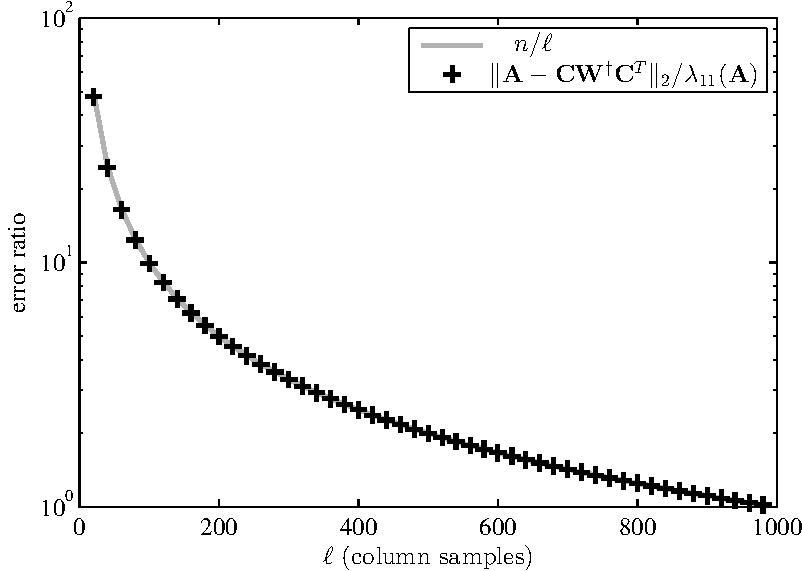
\includegraphics[width=6in,keepaspectratio=true]{%
figures/ch4/optimalityverification.pdf}
 \caption[Empirical demonstration of the optimality of Theorem~\ref{ch4:thm:uniformnystromerror}.]{
 {\sc Empirical demonstration of the optimality of Theorem~\ref{ch4:thm:uniformnystromerror}. } The empirical spectral-norm error of Nystr\"om extensions of
$\mat{A},$ the matrix defined in~\eqref{ch4:eqn:worsecaseA}, relative to the
spectral-norm error of the optimal rank-10 approximation of $\matA$. Each
point is the worst relative error observed in 60 trials. The ratio $n/\ell$ is
plotted; this is the dependence on $n$ and $\ell$ of the bound given in
Theorem~\ref{ch4:thm:uniformnystromerror}.}
 \label{ch4:fig:optimality}
\end{figure}


\subsection{Dependence on coherence}
In the following experiments, we use $500 \times 500$ matrices $\mat{A}$ with
eigendecompositions of the form
\begin{equation}
\mat{A} = [\begin{matrix} \mat{U}_1 & \mat{U}_2 \end{matrix}] 
 \left[ \begin{matrix} \mat{\Sigma}_1 & \\ & \mat{\Sigma}_2 \end{matrix} \right]
 \left[ \begin{matrix} \mat{U}_1\transp \\ \mat{U}_2\transp \end{matrix} \right]
 \label{ch4:eqn:coherenceA}
\end{equation}
where $\mat{U}_1$ is a $500 \times 10$ matrix with orthonormal columns and
specified coherence and the matrix $\mat{U}_2$ is chosen so that
$[\begin{matrix} \mat{U}_1 & \mat{U}_2 \end{matrix}]$ is an orthogonal matrix.
The 20 largest eigenvalues of $\mat{A}$ range logarithmically from $10$ to
$10^{-3},$ and the remaining eigenvalues are identically $10^{-15}.$ Routines
from the \textit{kappaSQ} Matlab package introduced in~\cite{IW12} are used to
generate $\mat{U}_1$ with specified coherences. For each value of coherence, we
consider two types of matrices $\mat{U}_1$ achieving this coherence: dense $\mat{U}_1$,
in which many rows of $\mat{U}_1$ are nonzero, and sparse $\mat{U}_1$, in which
many rows of $\mat{U}_1$ are zero. Dense $\mat{U}_1$ are generated using the
\texttt{mtxGenMethod1} routine, and sparse $\mat{U}_1$ are generated using the
\texttt{mtxGenMethod3} routine.

We compare the accuracies of regularized Nystr\"om extensions constructed using
Algorithm~\ref{ch4:alg:simple-stable-nystrom},
 to those of regularized Nystr\"om extensions constructed using
Algorithm~\ref{ch4:alg:CD11}. In Figure~\ref{ch4:fig:vary-coherence} we plot the ratio
of the approximation errors of the two regularized Nystr\"om extensions to the approximation
error of the optimal rank-10 approximant, as the coherence and sparsity of
$\mat{U}_1$ vary.
The regularization parameter $\rho$ is assigned the value
$\lambda_{11}(\mat{A}).$

\begin{figure}[htb!]
\centering
 \subfigure[Relative spectral-norm errors of
Algorithm~\ref{ch4:alg:simple-stable-nystrom}]{%
 
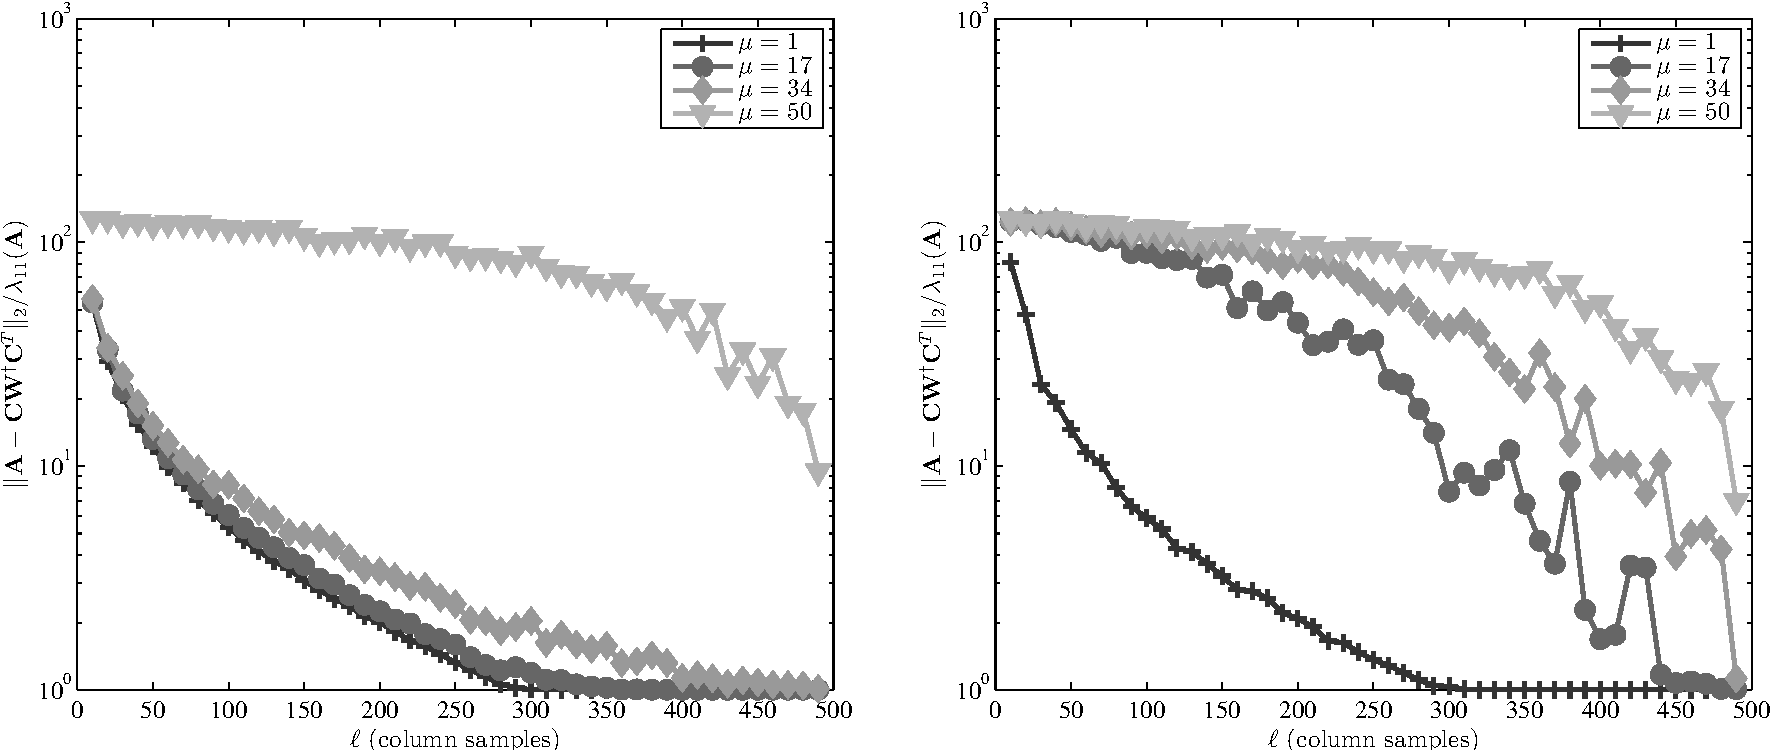
\includegraphics[height=2.3in,keepaspectratio=true]{%
figures/ch4/RegularizedADenseVsSparse.pdf}
}


\subfigure[Relative spectral-norm errors of Algorithm~\ref{ch4:alg:CD11}]{%
 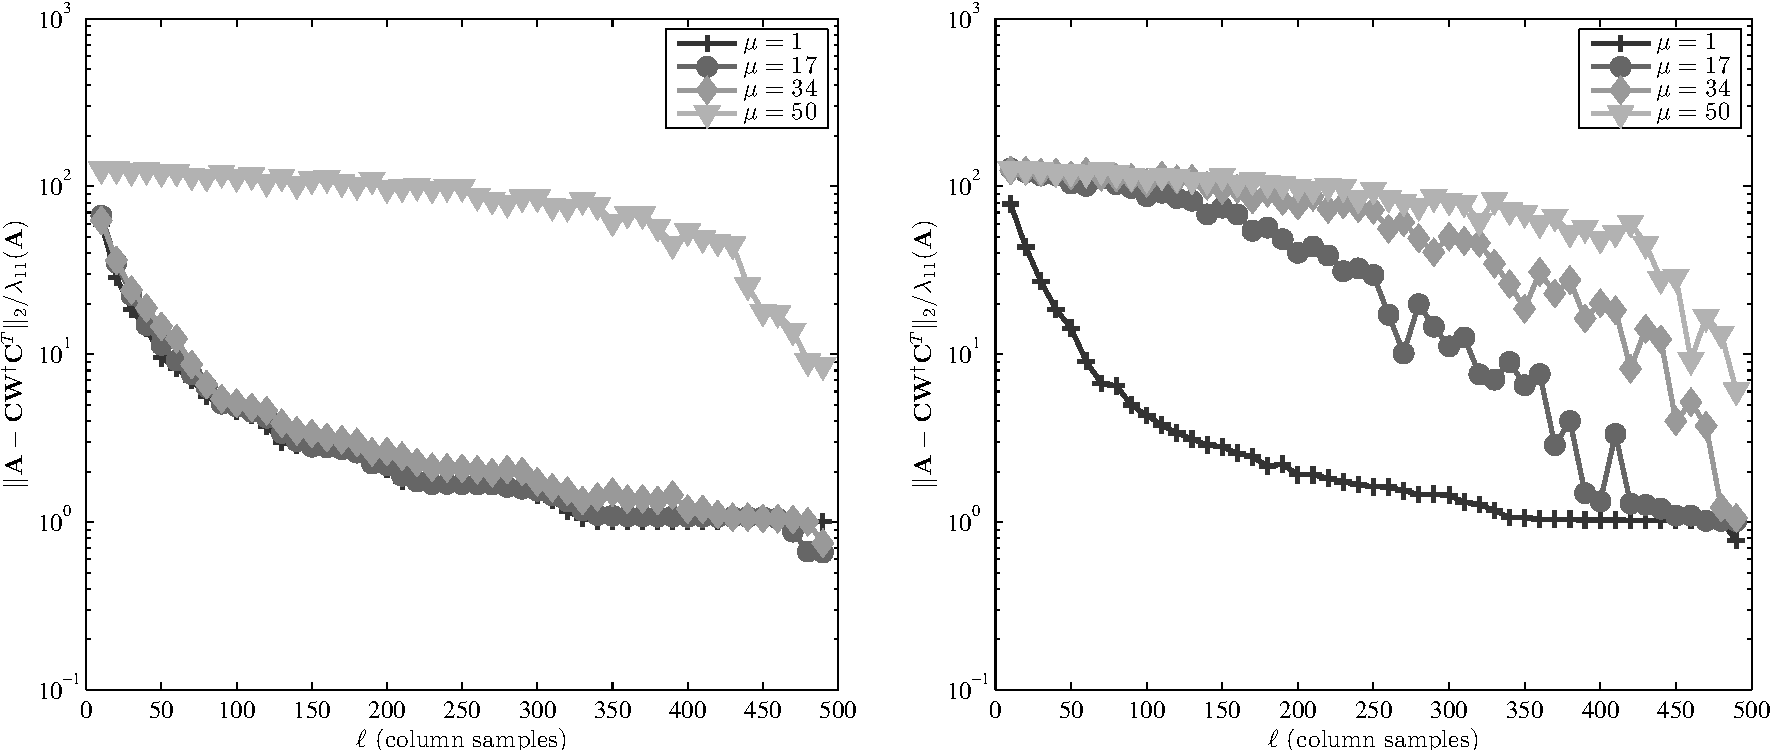
\includegraphics[height=2.3in,keepaspectratio=true]{%
figures/ch4/TruncatedWDenseVsSparse.pdf}
}

\caption[Spectral-norm errors of regularized Nystr\"om extensions as coherence varies]{%
{\sc Spectral-norm errors of regularized Nystr\"om extensions as coherence varies.} 
The relative spectral-norm errors of Nystr\"om extensions of $\mat{A},$
the matrix defined in~\eqref{ch4:eqn:coherenceA}, generated using
Algorithms~\ref{ch4:alg:simple-stable-nystrom} and~\ref{ch4:alg:CD11},
as a function of the coherence of the dominant
10-dimensional eigenspace. The errors are measured relative to the error of the
optimal rank-10 approximation, and averaged over 60 runs for each value of
$\ell.$ The eigenvectors spanning the dominant eigenspace of the matrices used
in the experiments on the left-hand side are dense, and the corresponding
eigenvectors of the matrices used in the experiments on the right-hand side are
sparse. The coherences range from the minimum possible, 1, to the maximum of
50.}
\label{ch4:fig:vary-coherence}
\end{figure}

Both algorithms perform as suggested by Theorem~\ref{ch4:thm:uniformnystromerror}: as the coherence of the top
$k$-dimensional eigenspace increases, the number of samples needed to obtain a small relative
error increases. Additionally, Figure~\ref{ch4:fig:vary-coherence} shows that the
structure of the eigenvectors is as important as the coherence of the
eigenspace: when the eigenvectors are dense, the number of samples needed to
obtain a small relative error is much less sensitive to the coherence than when
the eigenvectors are sparse. That is, for a fixed coherence and number of column
samples, the Nystr\"om extensions give lower errors when the eigenvectors are
dense than they do when the eigenvectors are sparse. 

\subsection*{Dependence on the regularization parameter}
Both algorithms require the choice of a regularization parameter
$\rho.$ In Figure~\ref{ch4:fig:regularization}, we observe the effect of the
regularization parameter $\rho$ on the errors of the Nystr\"om extensions. Here
the matrix $\mat{A}$ is again a $500 \times 500$ matrix with eigendecomposition
\begin{equation}
\mat{A} = [\begin{matrix} \mat{U}_1 & \mat{U}_2 \end{matrix}] 
 \left[ \begin{matrix} \mat{\Sigma}_1 & \\ & \mat{\Sigma}_2 \end{matrix} \right]
 \left[ \begin{matrix} \mat{U}_1\transp \\ \mat{U}_2\transp \end{matrix}
\right],
 \label{ch4:eqn:rhodependencematrix}
\end{equation}
where $\mat{U}_1$ is a $500 \times 20$ matrix with orthonormal columns and
$\mat{U}_2$ is chosen so that $[\begin{matrix} \mat{U}_1 & \mat{U}_2
\end{matrix}]$ is an orthogonal matrix. The 40 dominant eigenvalues of $\mat{A}$
range logarithmically from $1$ to $10^{-10}$ and all remaining eigenvalues are
identically $10^{-10}.$ The \texttt{mtxGenMethod1} routine is used to construct
$\mat{U}_1$ with coherence 1. 

Figure~\ref{ch4:fig:regularization} shows the ratios of the spectral-norm 
errors of the Nystr\"om extension and the regularized extensions
computed by Algorithms~\ref{ch4:alg:simple-stable-nystrom} and~\ref{ch4:alg:CD11}
to the optimal rank-20 approximation error. The
number of columns used to form the extensions is fixed at $\ell = 200,$ 
and the regularization parameter is varied from the minimum possible value of 
1 to the maximum possible value of 50. We see
that both regularization algorithms exhibit the same behavior: for large
values of $\rho,$ they have higher error than the Nystr\"om extension; as
$\rho$ decreases, their errors become orders of magnitude smaller than that of
the Nystr\"om extension, and as $\rho$ continues to decrease, their
errors once again approach that of the Nystr\"om extension. This behavior
highlights the importance of choosing an appropriate regularization parameter:
if $\rho$ is too small then there is no benefit gained from the regularization,
and if it is too large then the 
regularization has a deliterious effect. We also observe that Algorithm~\ref{ch4:alg:CD11}
can be orders of magnitude more accurate than Algorithm~\ref{ch4:alg:simple-stable-nystrom}.

\begin{figure}[ht]
 \centering
 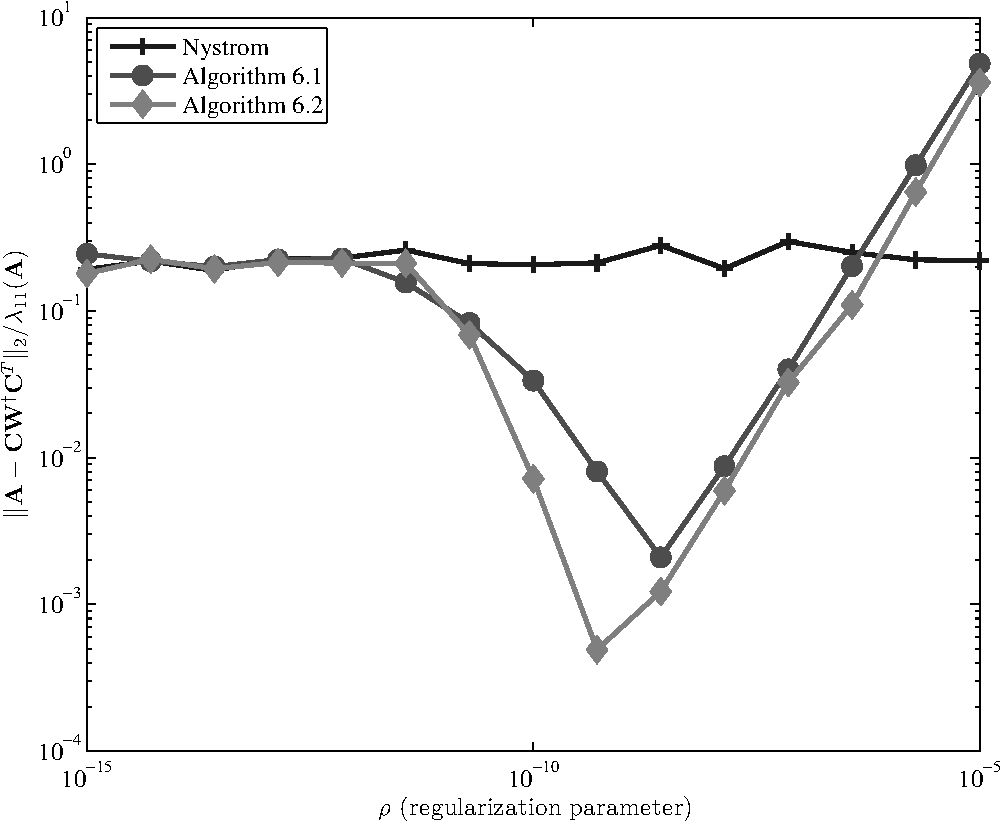
\includegraphics[width=6in,keepaspectratio=true]{%
figures/ch4/regularizationdependence.pdf}
 \caption[Spectral-norm error of regularized Nystr\"om extensions as regularization parameter varies]{%
{\sc Spectral-norm error of regularized Nystr\"om extensions as regularization parameter varies.} 
For the matrix $\mat{A}$ defined in~\eqref{ch4:eqn:rhodependencematrix},
the spectral-norm errors of the Nystr\"om extension and the extensions
generated using Algorithms~\ref{ch4:alg:simple-stable-nystrom}
and~\ref{ch4:alg:CD11}, as a function of
the regularization parameter $\rho.$ The errors are averaged over 60 runs for
each value of $\rho$ and plotted relative to the optimal spectral-norm rank-10 approximation error.}
 \label{ch4:fig:regularization}
\end{figure}


\section{Empirical aspects of SPSD low-rank approximation}
\label{ch4:sxn:emp}

In this section, we examine the empirical performance of the SPSD sketches
for which theoretical bounds were provided in Sections~\ref{ch4:sec:nystromextensions}
and~\ref{ch4:sec:mixturesketches}, on a diverse set of SPSD matrices.
% In addition to understanding the relative merits, in terms of both running 
% time and solution quality, of different sampling/projection schemes, we 
% would like to understand the effects of various data preprocessing decisions. 
% The bulk of our empirical evaluation considers two random projection
% procedures and two random sampling procedures for the sketching matrix 
% $\matS$:
% for random projections, we consider using SRFTs (Subsampled Randomized Fourier Transforms) as well as uniformly 
% sampling from Gaussian mixtures of the columns; and for random sampling, we 
% consider sampling columns uniformly at random as well as sampling 
% columns according to a nonuniform importance sampling distribution that 
% depends on the empirical statistical leverage scores.
% In the latter case of leverage score-based sampling, we also consider 
% the use of both the (na\"{i}ve and expensive) exact algorithm as well as 
% a (recently-developed fast) approximation algorithm.
%%
% Section~\ref{ch4:sxn:emp-datasets} starts with a brief description of 
% the data sets we consider; and then Section~\ref{ch4:sxn:emp-decisions} 
% briefly describes the effect of various data preprocessing decisions.
% Then, in Section~\ref{ch4:sxn:emp-reconstruction}, we present our main 
% results on reconstruction quality for the random sampling and random 
% projection methods; and, in Section~\ref{ch4:sxn:approx-levmethods}, we 
% discuss running time issues, and we present our main results for running time 
% and reconstruction quality for both exact and approximate versions of 
% leverage-based sampling.
% 
% We emphasize that we don't intend these results to be ``comprehensive'' but 
% instead to be ``illustrative'' case-studies---that are representative of a 
% much wider range of applications than have been considered previously.
% In particular, we would like to illustrate the tradeoffs between these 
% methods in different realistic applications in order, \emph{e.g.}, to provide 
% directions for future work.
% For instance, \emph{prima facie}, algorithms based on leverage-based column 
% sampling might be expected to be more expensive than those based on uniform 
% column sampling or random projections, but (based on previous work for general 
% matrices~\cite{DMM08CUR,DMMS11,MM11})
% they might also be expected to deliver lower approximation errors.
% Similarly, using approximate leverage scores to construct the importance 
% sampling distribution might be expected to perform worse than using exact 
% leverage scores, but this might be acceptable given its computational 
% advantages. 
% In addition to clarifying some of these issues, our empirical evaluation 
% also illustrates ways in which existing theory is insufficient to 
% explain the success of sampling and projection methods.
% This motivates our improvements to existing theory that we describe in 
% Section~\ref{sxn:theory}.

% With respect to our computation environment,
% all of our computations were conducted using 64-bit MATLAB R2012a under 
% Ubuntu on a 2.6--GHz quad-core Intel i7 machine with 6Gb of RAM. 
% To allow for accurate timing comparisons, all computations were carried out 
% in a single thread. 
% When applied to an $n \times n$ SPSD matrix $\mat{A}$, 
% our implementation of the SRFT requires $\mathrm{O}(n^2 \log n)$ operations, 
% as it applies MATLAB's \texttt{fft} to the entire matrix $\mat{A}$ and
% \emph{then} it samples $\ell$ columns from the resulting matrix. 
% We note that the SRFT computation can be made more competitive: a more rigorous 
% implementation of the SRFT algorithm could reduce this running time to 
% $\mathrm{O}(n^2 \log \ell)$; but due to the complexities involved in 
% optimizing pruned FFT codes, we did not pursue this~avenue. 


\subsection{Test matrices}
\label{ch4:sxn:emp-datasets}

Table~\ref{ch4:table:datasets} provides summary statistics for the test matrices used 
in our computational experiments. 
In order to illustrate the strengths and weaknesses of 
% the different sketches over a wide range of matrices, we consider four classes of matrices which are commonly 
encountered in machine learning and data analysis applications, we drawn our test
matrices from the following classes of matrices: 
\begin{itemize}
\item normalized Laplacians of very sparse graphs drawn from ``informatics graph'' 
applications;
\item dense matrices corresponding to linear kernels from machine learning 
applications;
\item dense matrices constructed from a Gaussian radial basis function kernel 
(RBFK); and
\item sparse RBFK matrices constructed using Gaussian radial basis functions, 
truncated to be nonzero only for nearest neighbors.
\end{itemize}
% Although not exhaustive, this collection of data sets represents a wide range of 
% data sets with very different (sparsity, spectral, leverage score, etc.) 
% properties that have been of interest recently not only in machine learning 
% but in data analysis more generally.

\begin{table}[t]
\centerline{%
\begin{tabular}{|l|c|l|l|l|}
\hline
Name & Description & n & d  & \%nnz \\
\hline
\hline
\multicolumn{4}{|c|}{Laplacian kernels} \\
\hline
HEP      & arXiv High Energy Physics collaboration graph & 9877  & NA  & 0.06 \\
GR       & arXiv General Relativity collaboration graph  & 5242  & NA  & 0.12 \\
Enron    & subgraph of the Enron email graph             & 10000 & NA  & 0.22 \\
Gnutella & Gnutella peer to peer network on Aug. 6, 2002 & 8717  & NA  & 0.09 \\
\hline
\hline
\multicolumn{3}{|c|}{Linear kernels} \\
\hline
Dexter  & bag of words                             & 2000 & 20000  & 83.8 \\
Protein & derived feature matrix for S. cerevisiae & 6621 & 357    & 99.7 \\
SNPs    & DNA microarray data from cancer patients & 5520 & 43     & 100 \\
Gisette & images of handwritten digits             & 6000 & 5000   & 100 \\
\hline
\hline
\multicolumn{3}{|c|}{Dense RBF kernels} \\
\hline
AbaloneD & physical measurements of abalones & 4177 & 8   & 100 \\
WineD    & chemical measurements of wine     & 4898 & 12  & 100 \\
%Kin8nm   & simulated dynamics of a robot arm & 8192 & 9   & 100 \\
%Spam     & word and character frequencies    & 4601 & 57  & 100 \\
\hline
\hline
\multicolumn{3}{|c|}{Sparse RBF kernels} \\
\hline
AbaloneS & physical measurements of abalones & 4177 & 8  & 82.9/48.1 \\
WineS    & chemical measurements of wine     & 4898 & 12 & 11.1/88.0 \\
\hline
\end{tabular}
}
\caption[Information on the SPSD matrices used in our empirical evaluations]{
{\sc Information on the SPSD matrices used in our empirical evaluations.} The matrices used in our empirical evaluation 
(\cite{LKF07}, \cite{KY04}, \cite{GGBD05}, \cite{GSPDK06}, 
\cite{Netal02}, \cite{Corke96}, \cite{UCIMachineLearningRepository}). 
Here, $n$ is the number of data points, and $d$ is the number of features in 
the input space before kernelization.
For Laplacian ``kernels,'' $n$ is the number of nodes in the graph (and thus 
there is no $d$ since the graph is ``given'' rather than ``constructed'').
The \%nnz for the Sparse RBF kernels depends on the $\sigma$ parameter; 
see Table~\ref{ch4:table:datasets_stats}.
}
\label{ch4:table:datasets}
\end{table}


We briefly review the construction of normalized graph Laplacians, 
linear kernel matrices, RBFK matrices, and sparse RBFK matrices.

Given a graph with weighted adjacency matrix $\mat{W}$, its normalized graph Laplacian is 
\[
  \mat{A} = \mat{I} - \mat{D}^{-1/2} \mat{W} \mat{D}^{-1/2},
\]
where $\mat{D}$ is the diagonal matrix of weighted degrees of the nodes of the
graph, i.e., $D_{ii} = \sum_{j \neq i} W_{ij}$.

The remaining classes of matrices are constructed using a set of 
data points $\vec{x}_1, \ldots, \vec{x}_n \in \R^d.$ The linear kernel 
matrix $\mat{A}$ corresponding to those points is given by
\[
 A_{ij} = \langle \vec{x}_i, \vec{x}_k \rangle.
\]
A Gaussian RBFK matrix $\mat{A}^\sigma$ corresponding to these same points
is given by
\[
 A_{ij}^\sigma = \exp\bigg(\frac{-\TNormS{\vec{x}_i -
\vec{x}_j}}{\sigma^2}\bigg),
\]
where $\sigma$, a nonnegative number, determines the scale of the kernel.
Informally, $\sigma$ defines the ``size scale'' over which pairs of 
points $\vec{x}_i$ and $\vec{x}_j$ ``see'' each other.
Typically $\sigma$ is determined by a global cross-validation criterion, as 
$\mat{A}^\sigma$ is generated for some specific machine learning task. Thus,
one may have no \emph{a priori} knowledge of the behavior of the 
spectrum or leverage scores of $\mat{A}^\sigma$ as $\sigma$ is varied. 
Accordingly, we consider Gaussian RBFK matrices with different values of $\sigma$. 
Finally, given the same data points, one
can construct sparse Gaussian RBFK matrices using the formula
\[
 A_{ij}^{(\sigma,\nu,C)} = \left[ \left( 1 - \frac{\TNorm{\vec{x}_i 
 - \vec{x}_j}}{C}\right)^\nu \right]^+ \cdot \exp\bigg(\frac{-\TNormS{\vec{x}_i -
\vec{x}_j}}{\sigma^2}\bigg),
\]
where $[x]^+ = \max\{0, x\}.$
When $\nu$ is larger than $(d+1)/2,$ this matrix is positive semidefinite; 
and as the cutoff point $C$ decreases this matrix becomes more 
sparse~\cite{Genton02}. 
For simplicity, in our experiments we fix 
$\nu = \lceil (d+1)/2 \rceil$ and $C = 3 \sigma$ and we vary $\sigma$.
As with the effect of varying $\sigma$, the effect of varying the 
sparsity parameter $C$ is not obvious \emph{a priori}. The parameter $C$ is typically chosen
according to a global criterion to ensure good performance at a specific machine learning 
task, without consideration for its effect on the spectrum or leverage 
scores of $A_{ij}^{(\sigma,\nu,C)}$.

\begin{table}[t]
\small
\centerline{%
\begin{tabular}{|l|l|l|l|l|l|l|}
\hline
Name & \%nnz 
     & $\Big\lceil\tfrac{\FNormS{\mat{A}}}{\TNormS{\mat{A}}} \Big\rceil$
     & $k$ 
     & $\tfrac{\lambda_{k+1}}{\lambda_k}$ 
     & $100 \tfrac{\FNorm{\mat{A} - \mat{A}_k}}{\FNorm{\mat{A}}}$  
     & \pbox{3cm}{$k$th-largest \\ leverage score} \\
\hline
\hline
% Laplacian data sets
HEP & 0.06 & 3078 & 20 & 0.998 & 7.8 & 0.261 \\ 
HEP & 0.06 & 3078 & 60 & 0.998 & 13.2 & 0.278 \\
GR & 0.12 & 1679 & 20 & 0.999 & 10.5 & 0.286 \\
GR & 0.12 & 1679 & 60 & 1 & 17.9  & 0.289 \\
Enron & 0.22 & 2588 & 20 & 0.997 & 7.77 & 0.492 \\
Enron & 0.22 & 2588 & 60 & 0.999 & 12.0 & 0.298 \\
Gnutella & 0.09 & 2757 & 20 & 1 & 8.1 & 0.381 \\
Gnutella & 0.09 & 2757 & 60 & 0.999 & 13.7 & 0.340 \\
\hline
\hline
% Linear data sets
Dexter  & 83.8 & 176 & 8  & 0.963 & 14.5 & 0.067 \\
Protein & 99.7 & 24  & 10 & 0.987 & 42.6 & 0.008 \\
SNPs    & 100  & 3   & 5  & 0.928 & 85.5 & 0.002 \\
Gisette & 100  & 4   & 12 & 0.90  & 90.1 & 0.005 \\
\hline
\hline
% Dense RBF data sets
AbaloneD (dense, $\sigma = .15$) & 100 & 41 & 20 & 0.992 & 42.1 & 0.087 \\
AbaloneD (dense, $\sigma = 1$)   & 100 & 4  & 20 & 0.935 & 97.8 & 0.012 \\
WineD (dense, $\sigma = 1$)      & 100 & 31 & 20 & 0.99  & 43.1 & 0.107 \\
WineD (dense, $\sigma = 2.1$)    & 100 & 3  & 20 & 0.936 & 94.8 & 0.009 \\
\hline
\hline
% Sparse RBF data sets
AbaloneS (sparse, $\sigma = .15$) & 82.9 & 400 & 20 & 0.989 & 15.4 & 0.232 \\
AbaloneS (sparse, $\sigma = 1$)   & 48.1 & 5   & 20 & 0.982 & 90.6 & 0.017 \\
WineS (sparse, $\sigma = 1$)      & 11.1 & 116 & 20 & 0.995 & 29.5 & 0.200 \\
WineS (sparse, $\sigma = 2.1$)    & 88.0   & 39  & 20 & 0.992 & 41.6 & 0.098 \\
\hline
\end{tabular}
}
\caption[Statistics of our test matrices]{{\sc Statistics of our test matrices.}
Summary statistics for the matrices from Table~\ref{ch4:table:datasets}
used in our computational experiments.}
\label{ch4:table:datasets_stats}
\end{table}

To illustrate the diverse range of properties exhibited by these four classes
of matrices, consider Table~\ref{ch4:table:datasets_stats}.
Several observations are particularly relevant to our
discussion below.
\begin{itemize}
\item
All of the Laplacian kernels drawn from informatics graph applications are 
extremely sparse in terms of number of nonzeros, and tend to have 
very slow spectral decay, as illustrated both by the quantity 
$\big\lceil\FNormS{\mat{A}}/\TNormS{\mat{A}}\big\rceil$ (this is the 
\emph{stable rank}, a numerically stable (under)estimate of the 
rank of $\mat{A}$ also utilized in Chaper~\ref{ch3}) as well as by the relatively small fraction of the 
Frobenius norm that is captured by the best rank-$k$ approximation to 
$\mat{A}$.
For the Laplacian kernels we considered two values of the rank parameter $k$ 
that were chosen (somewhat) arbitrarily; many of the results we report 
continue to hold qualitatively if $k$ is chosen to be (say) an order of 
magnitude larger. % but doing so tends to densify the low-rank approximation 
%to the Laplacian matrix.
\item
Both the linear kernels and the dense RBF kernels are much denser and are 
much more well-approximated by moderate to very low-rank matrices.
In addition, both the linear kernels and the dense RBF kernels have 
statistical leverage scores that are much more uniform---there are several 
ways to illustrate this, none of them perfect, and here, we illustrate this 
by considering the $k$th largest leverage score.
For the linear kernels and the dense RBF kernels, this quantity is one to
two orders of magnitude smaller than for the Laplacian kernels.
\item
For the dense RBF kernels, we consider two values of the $\sigma$ parameter, 
again chosen (somewhat) arbitrarily.
For both AbaloneD and WineD, we see that decreasing $\sigma$ from $1$ to 
$0.15$, i.e., letting data points ``see'' fewer nearby points, has two 
important effects:
first, it results in matrices that are much less well-approximated by 
low-rank matrices; and
second, it results in matrices that have much more heterogeneous leverage 
scores.
For example, for AbaloneD, the fraction of the Frobenius norm that is captured 
decreases from $97.8$ to $42.1$ and the $k$th largest leverage score 
increases from $0.012$ to~$0.087$.
\item
For the sparse RBF kernels, there are a range of sparsities, ranging from
above the sparsity of the sparsest linear kernel, but all are denser
than the Laplacian kernels.
Changing the $\sigma$ parameter has the same effect (although it is even 
more pronounced) for sparse RBF kernels as it has for dense RBF kernels.
In addition, ``sparsifying'' a dense RBF kernel also has the effect of 
making the matrix less well approximated by a low-rank matrix and of making
the leverage scores more nonuniform.
For example, for AbaloneD with $\sigma=1$ (respectively, $\sigma=0.15$), 
the fraction of the Frobenius norm that is captured decreases from $97.8$ 
(respectively, $42.1$) to $90.6$ (respectively, $15.4$), 
and the $k$th largest leverage score increases from $0.012$ 
(respectively, $0.087$) to $0.017$ (respectively,~$0.232$).
\end{itemize}
As we see below, when we consider the RBF kernels as the width parameter 
and sparsity are varied, we observe a range of intermediate cases between 
the extremes of linear kernels and Laplacian kernels.


\subsection{A comparison of empirical errors with the theoretical error bounds}

Table~\ref{ch4:table:theory-practice-gap} illustrates the gap between the theoretical results 
currently available in the literature, the bounds derived in this chapter, and what is observed in practice: it depicts the ratio
between the error bounds summarized in Table~\ref{ch4:table:bounds-comparison} and the average errors observed
over 10 trials of SPSD sketching. The error bound from~\cite{RT10} is not considered in the table,
as it does not apply at the number of samples $\ell$ used in the experiments. 

Several trends can be identified; among them, we
note that the bounds provided in this chapter for Gaussian-based sketches come quite close to capturing 
the errors seen in practice, and the Frobenius and trace-norm error guarantees of the 
leverage-based and Fourier-based sketches tend to more closely reflect the empirical behavior than
the error guarantees provided in prior work for Nystr\"om sketches. Overall, the trace-norm error
bounds are quite accurate. On the other hand, prior bounds are sometimes more informative in the case 
of the spectral norm (with the notable exception of the Gaussian sketches). Several important points
can be gleaned from these observations. 

First, the accuracy of the Gaussian error bounds suggests that the main theoretical
contribution of this work, the deterministic structural results given as 
Theorems~\ref{ch4:thm:colselection}, \ref{ch4:thm:frobenius-deterministic-error},
and~\ref{ch4:thm:trace-deterministic-error}, captures the underlying behavior of the SPSD sketching process. 
This supports our belief that our deterministic framework provides a foundation for truly 
informative error bounds. Second, it is clear that the 
analysis of the stochastic elements of the SPSD sketching process is 
much sharper in the Gaussian case than in the 
leverage-score, Fourier, and Nystr\"om cases. We expect that, at least in the 
case of leverage and Fourier-based sketches, the 
stochastic analysis can and will be sharpened to produce error guarantees 
almost as informative as the ones we have provided for
Gaussian-based sketches.

\begin{table}[!htb]
\centering
\begin{tabular}{|l|p{1in}|p{1in}|p{1in}|}
\hline
source, sketch
 & pred./obs. \linebreak spec. error
 & pred./obs. \linebreak Frob. error
 & pred./obs. \linebreak trace error \\
  \hline
  \multicolumn{4}{|c|}{Enron, $k = 60$ } \\
  \hline
% \cite{DM05}, Nystr\"om
%  & 3041
%  & 66.2
%  & -- \\
\cite{BW09}, Nystr\"om
 & --  
 & --  
 & 2.0\\
%\cite{TalRos10}, Nystr\"om
% & NA
% & NA
% & NA \\
\cite{KMT12}, Nystr\"om
 & 331.2
 & 77.7
 & -- \\
 Thm~\ref{ch4:thm:sample-lev},  leverage-based
 & 12888
 & 21
 & 1.2 \\
Thm~\ref{ch4:thm:proj-fourier}, Fourier-based
 & 201.0
 & 42.7
 & 1.6 \\
Thm~\ref{ch4:thm:proj-gaussian}, Gaussian-based
 & 10.1
 & 5.6
 & 1.2 \\
Thm~\ref{ch4:thm:uniformnystromerror}, Nystr\"om
 & 9.4
 & 385.2
 & 5.4 \\
 \hline
 \multicolumn{4}{|c|}{Protein, $k = 10$ }\\
 \hline
% \cite{DM05}, Nystr\"om
%  & 119.2 
%  & 18.6
%  & -- \\
\cite{BW09}, Nystr\"om
 & --  
 & --  
 & 3.6\\
%\cite{TalRos10}, Nystr\"om
% & NA
% & NA
% & NA \\
\cite{KMT12}, Nystr\"om
 & 33.4
 & 20.5
 & -- \\
Thm~\ref{ch4:thm:sample-lev},  leverage-based
 & 42.5
 & 6.9
 & 2.0 \\
Thm~\ref{ch4:thm:proj-fourier}, Fourier-based
 & 297.5
 & 21.7
 & 3.1\\
Thm~\ref{ch4:thm:proj-gaussian}, Gaussian-based
 & 3.8
 & 3.3
 & 1.8 \\
Thm~\ref{ch4:thm:uniformnystromerror}, Nystr\"om
 & 86.3
 & 91.3
 & 8 \\
 \hline
 \multicolumn{4}{|c|}{AbaloneD, $\sigma = .15, k = 20$ } \\
 \hline
% \cite{DM05}, Nystr\"om
%  & 349.9
%  & 42.5
%  & -- \\
\cite{BW09}, Nystr\"om
 & --  
 & --  
 & 2.0 \\
%\cite{TalRos10}, Nystr\"om
% & NA
% & NA
% & NA \\
\cite{KMT12}, Nystr\"om
 & 62.9
 & 46.7
 & -- \\
Thm~\ref{ch4:thm:sample-lev},  leverage-based
 & 235.3
 & 14.6
 & 1.3 \\
Thm~\ref{ch4:thm:proj-fourier}, Fourier-based
 & 139.4
 & 36.9
 & 1.7\\
Thm~\ref{ch4:thm:proj-gaussian}, Gaussian-based
 & 5.2
 & 4.7
 & 1.1\\
Thm~\ref{ch4:thm:uniformnystromerror}, Nystr\"om
 & 12.9
 & 228.3
 & 5.1\\
 \hline
 \multicolumn{4}{|c|}{WineS, $\sigma = 1, k = 20$ }\\
 \hline
%  \cite{DM05}, Nystr\"om
%  & 422.5
%  & 41.0
%  & -- \\
\cite{BW09}, Nystr\"om
 & --  
 & --  
 & 2.1\\
%\cite{TalRos10}, Nystr\"om
% & NA
% & NA
% & NA \\
\cite{KMT12}, Nystr\"om
 & 72.8
 & 44.2
 & -- \\
Thm~\ref{ch4:thm:sample-lev},  leverage-based
 & 244.9
 & 13.4
 & 1.2\\
Thm~\ref{ch4:thm:proj-fourier}, Fourier-based
 & 186.7
 & 36.8
 & 1.7\\
Thm~\ref{ch4:thm:proj-gaussian}, Gaussian-based
 & 6.6
 & 4.7
 & 1.2\\
Thm~\ref{ch4:thm:uniformnystromerror}, Nystr\"om
 & 13.7
 & 222.6
 & 5.1\\
 \hline
\end{tabular}
\caption[Comparison of empirical errors of SPSD sketches with predicted errors]{
{\sc Comparison of empirical errors of SPSD sketches with predicted errors.}
We compare the empirically observed approximation errors to the guarantees provided in this and other works, for several
matrices. Each approximation was formed using $\ell = 6 k\log k$ samples. To evaluate the error guarantees,
$\delta = 1/2$ was taken and all constants present in the statements of the bounds were replaced with ones. The observed errors were
taken to be the average errors over 10 runs of the approximation algorithms.
The matrices, described in Table~\ref{ch4:table:datasets}, are representative of several classes of matrices prevalent
in machine learning applications.}
\label{ch4:table:theory-practice-gap}
\end{table}


\subsection{Reconstruction accuracy of sampling and projection-based sketches}
\label{ch4:sxn:emp-reconstruction}

Here, we describe the performances of the various SPSD sketches in terms of 
reconstruction accuracy on the matrices described in 
Section~\ref{ch4:sxn:emp-datasets}. Recall that the sketches considered are
Nystr\"om extensions, leverage-based sketches, and sketches formed using 
Gaussian and SRFT mixtures of columns.

We describe general observations we have made about each class of 
matrices in turn, and then we summarize our observations.
We present results for both the rank-restricted and non-rank-restricted sketches.
That is, we plot the errors
\begin{equation}
\|\mat{A} - \mat{C} \mat{W}^\dagger \mat{C}\transp\|_\xi/\|\mat{A} - \mat{A}_k\|_\xi
\label{ch4:eqn:relerr1}
\end{equation}
for the non-rank-restricted sketches, and the errors 
\begin{equation}
\|\mat{A} - \mat{C} \mat{W}_k^\dagger \mat{C}\transp\|_\xi/\|\mat{A} - \mat{A}_k\|_\xi
\label{ch4:eqn:relerr2}
\end{equation}
for the rank-restricted sketches.

\subsubsection{Graph Laplacians}

\begin{figure}[htp]
 \centering
 \subfigure[GR, $k = 20$]{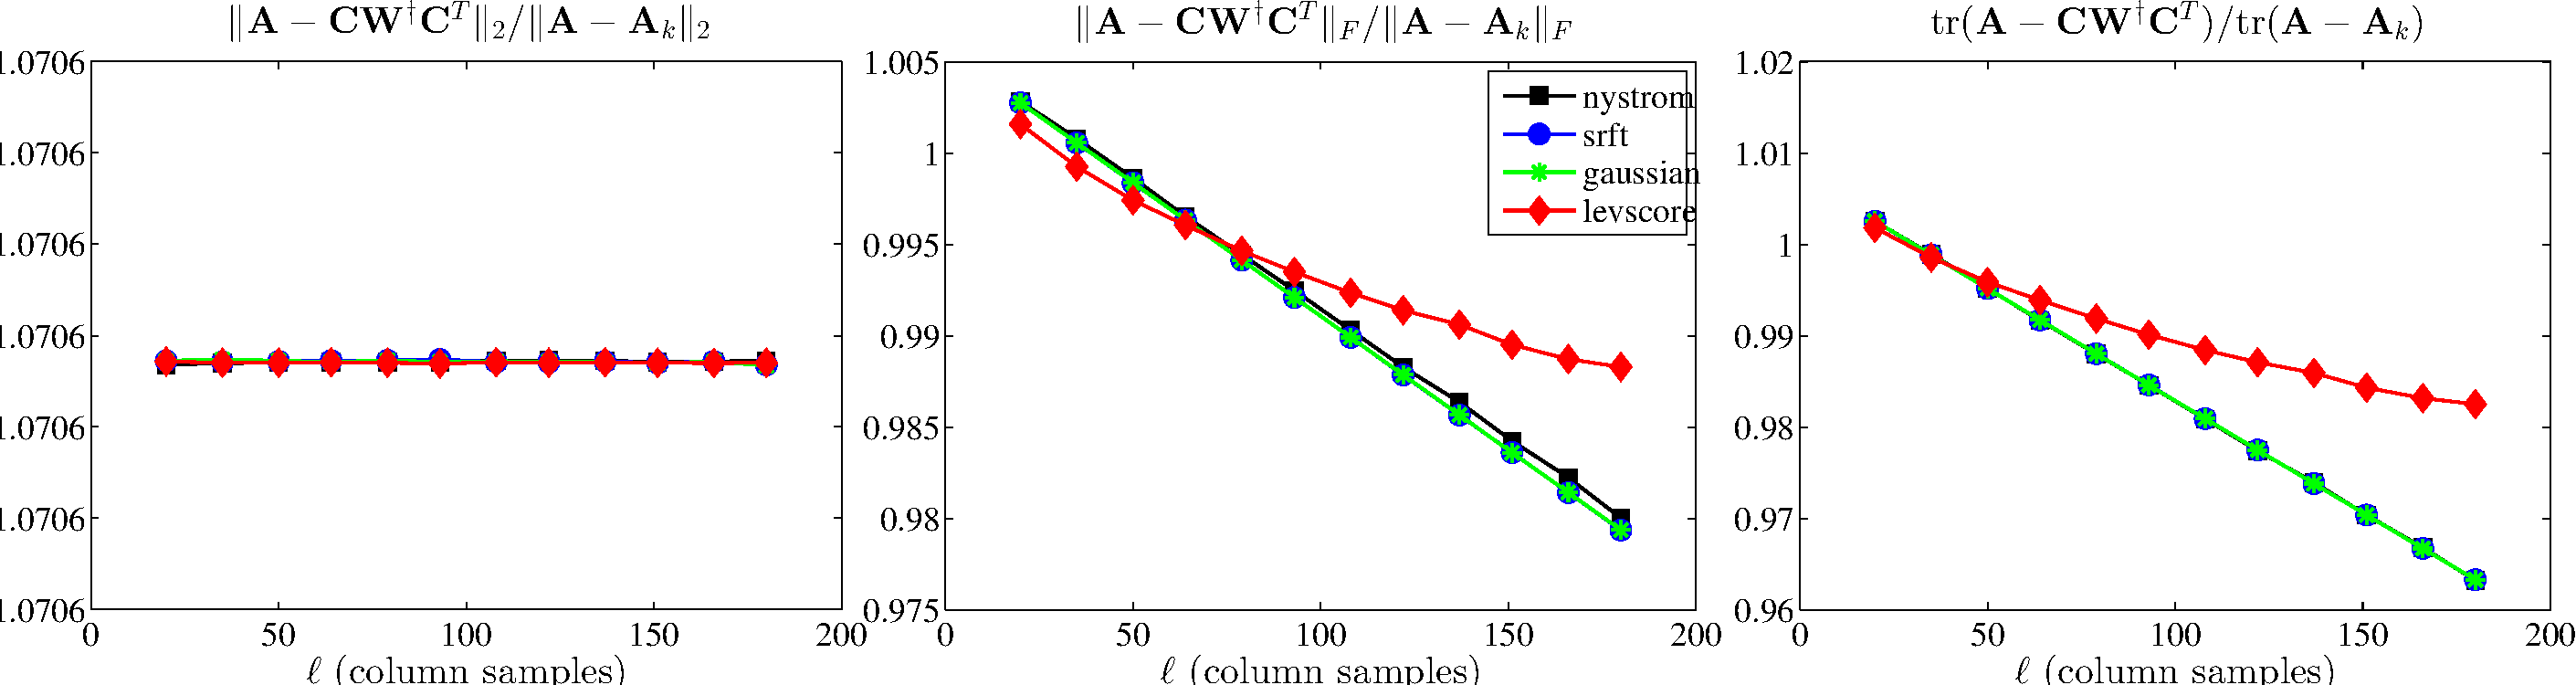
\includegraphics[width=6in, keepaspectratio=true]{figures/ch4/GRrank20exact-methods-nonfixed-rank-errors}}
 
 \subfigure[GR, $k = 60$]{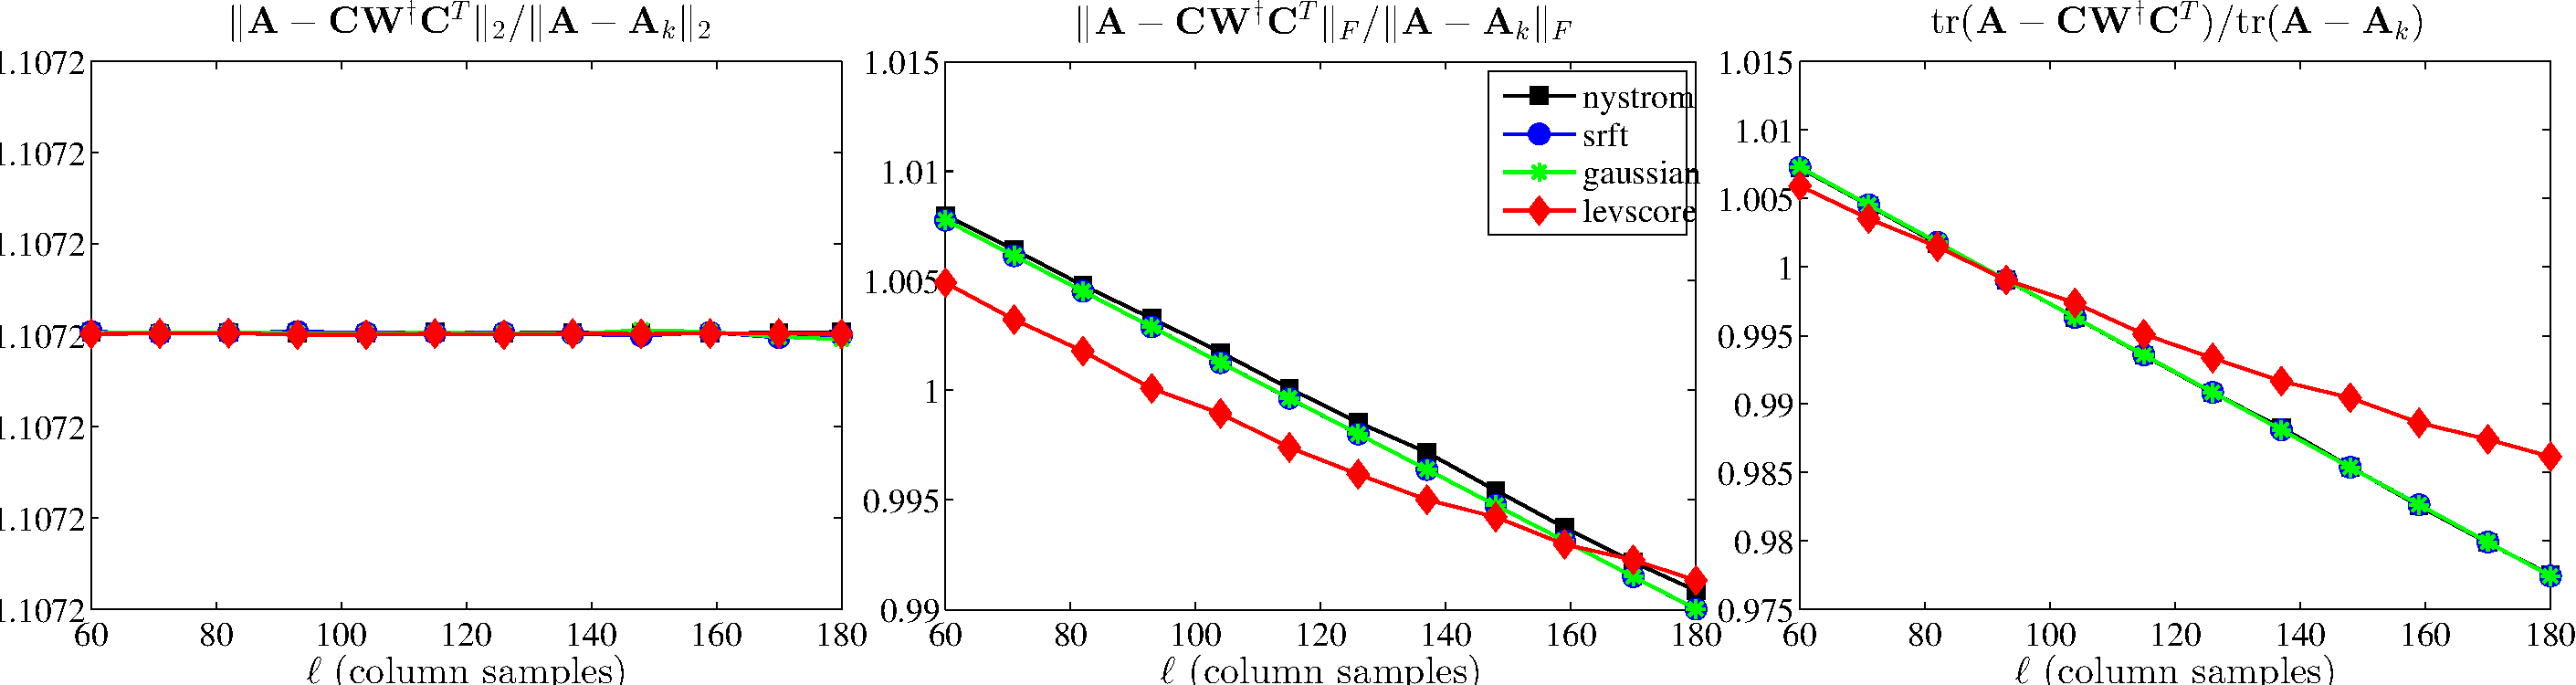
\includegraphics[width=6in, keepaspectratio=true]{figures/ch4/GRrank60exact-methods-nonfixed-rank-errors}}
 
 \subfigure[HEP, $k = 20$]{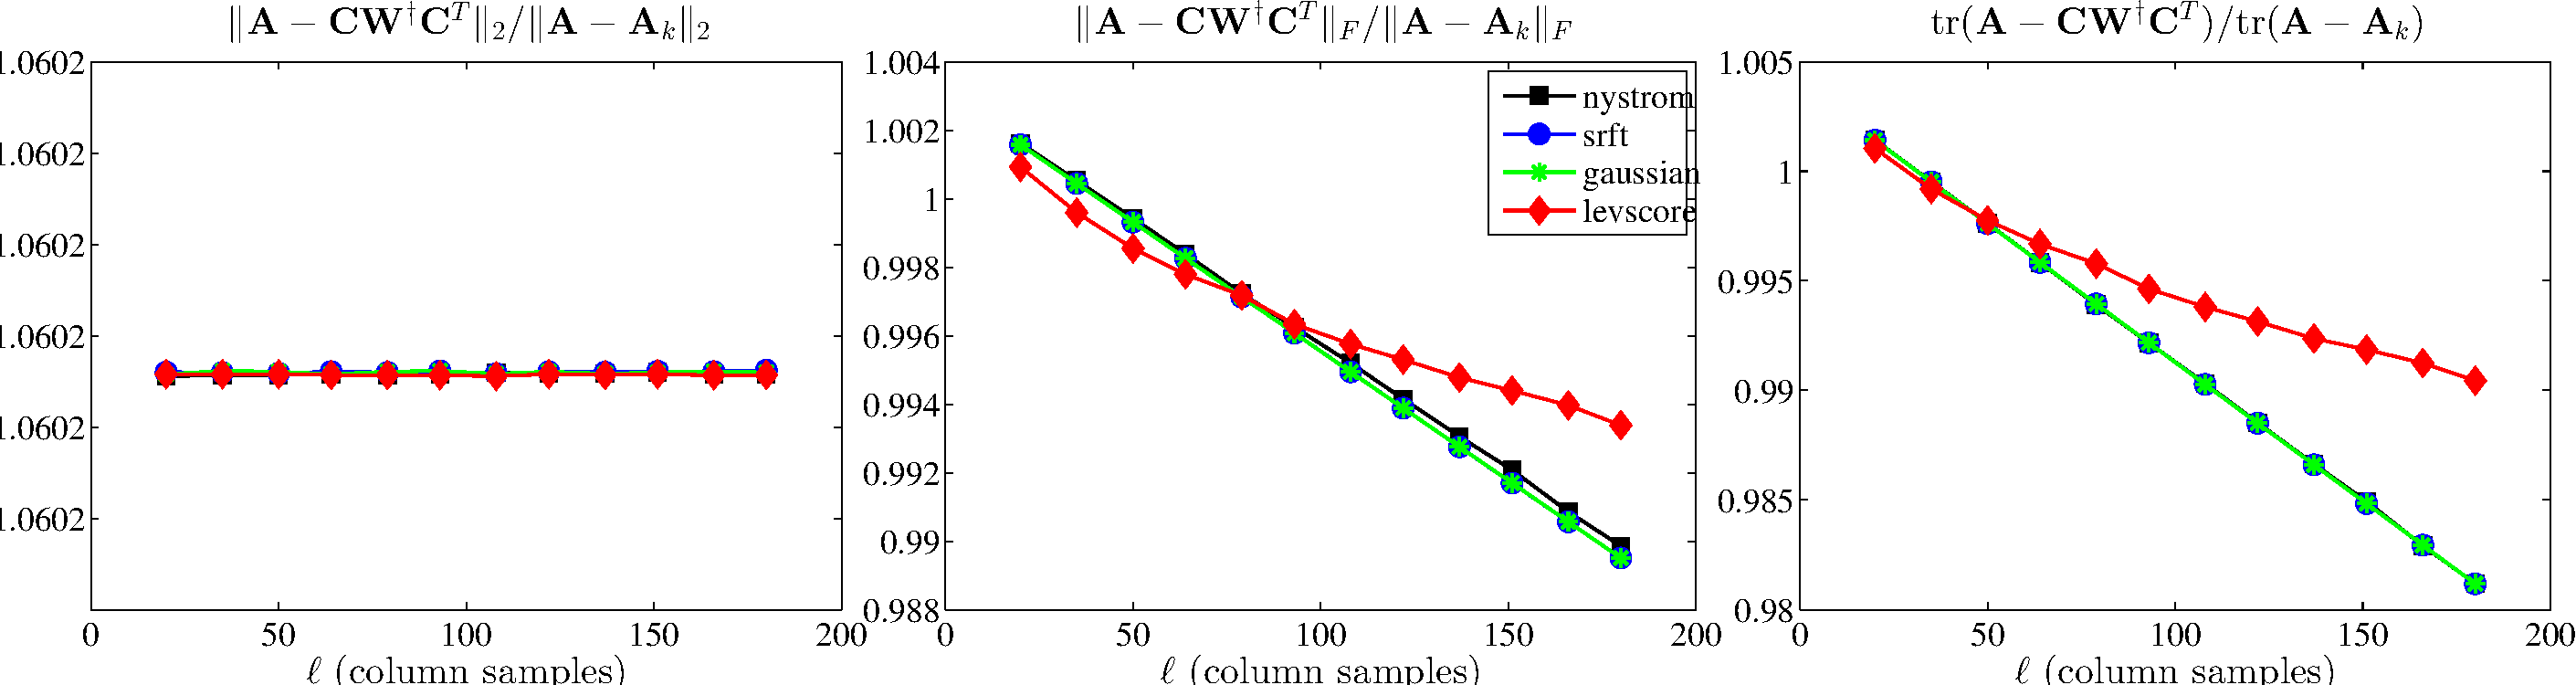
\includegraphics[width=6in, keepaspectratio=true]{figures/ch4/HEPrank20exact-methods-nonfixed-rank-errors}}
 
 \subfigure[HEP, $k = 60$]{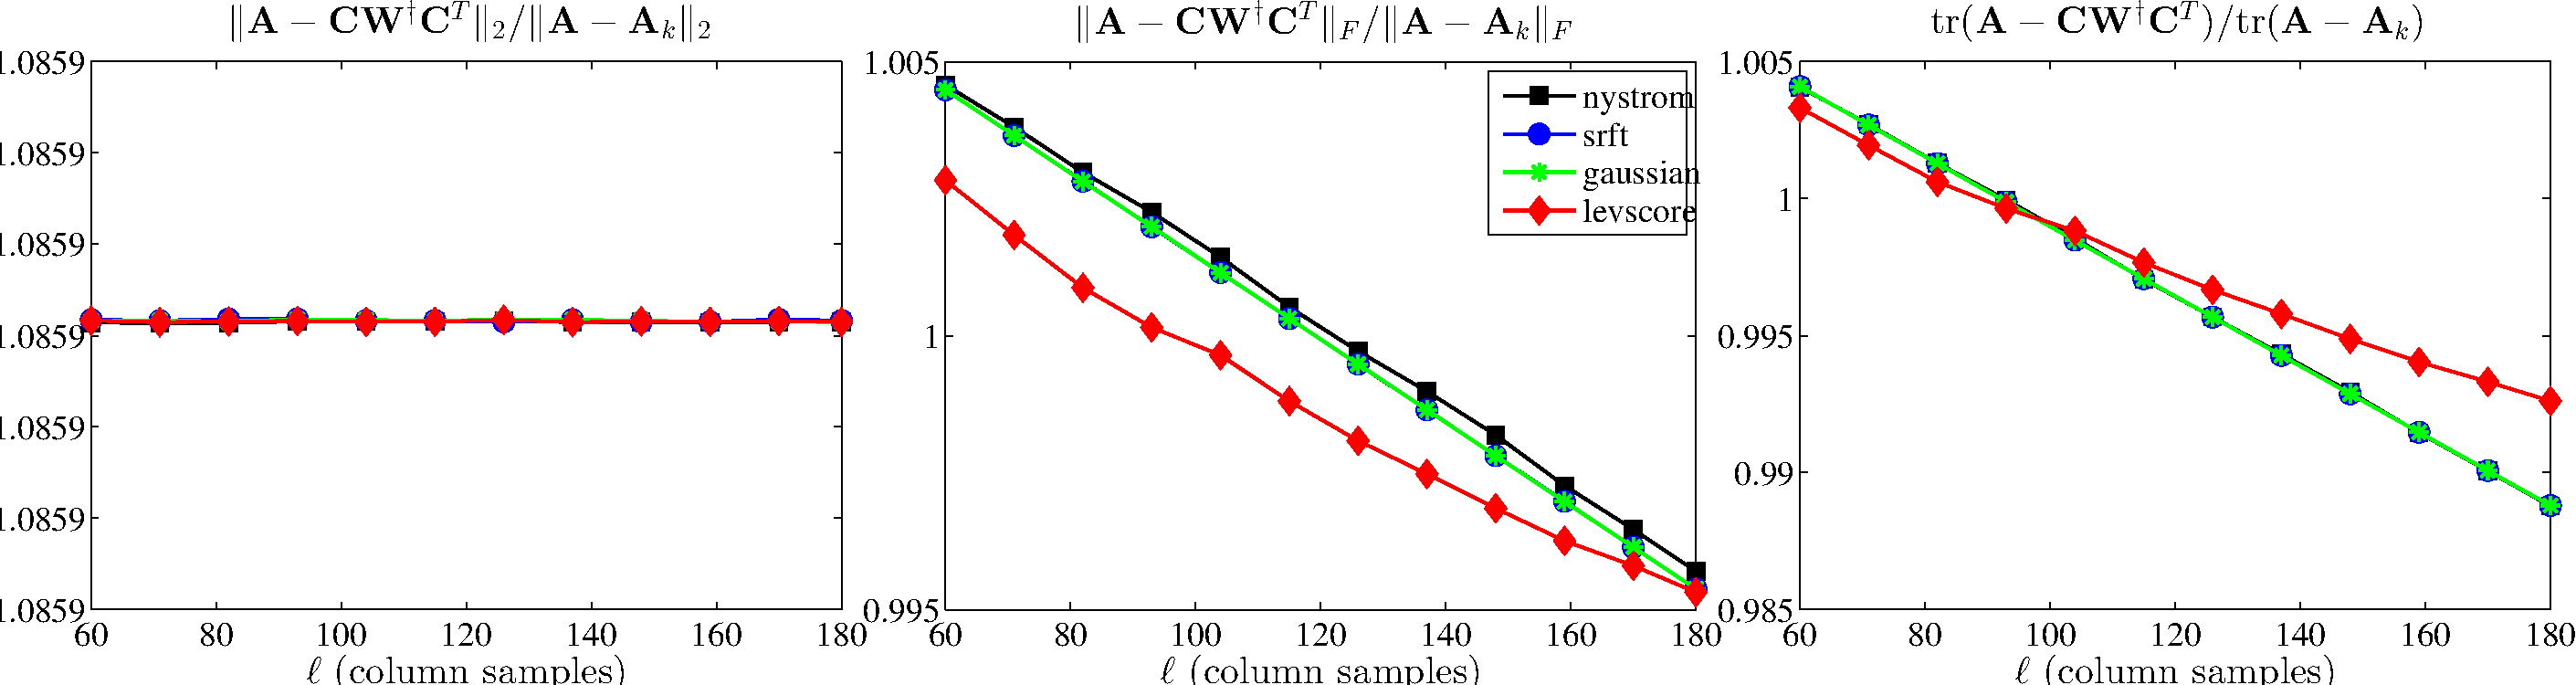
\includegraphics[width=6in, keepaspectratio=true]{figures/ch4/HEPrank60exact-methods-nonfixed-rank-errors}}%
  \caption[Relative errors of non-rank-restricted SPSD sketches of the GR and HEP Laplacian matrices]{%
 {\sc Relative errors of non-rank-restricted SPSD sketches of the GR and HEP Laplacian matrices.}
 The relative spectral, Frobenius, and trace-norm errors~\eqref{ch4:eqn:relerr1} of several non-rank-restricted
 SPSD sketches, as a function of the number of columns samples $\ell$, 
 for the GR and HEP Laplacian matrices, with two choices of the rank parameter $k$.}%
 \label{ch4:fig:laplacian-exact-errors-1a}
\end{figure}

\begin{figure}[htp]
 \centering
 \subfigure[Enron, $k = 20$]{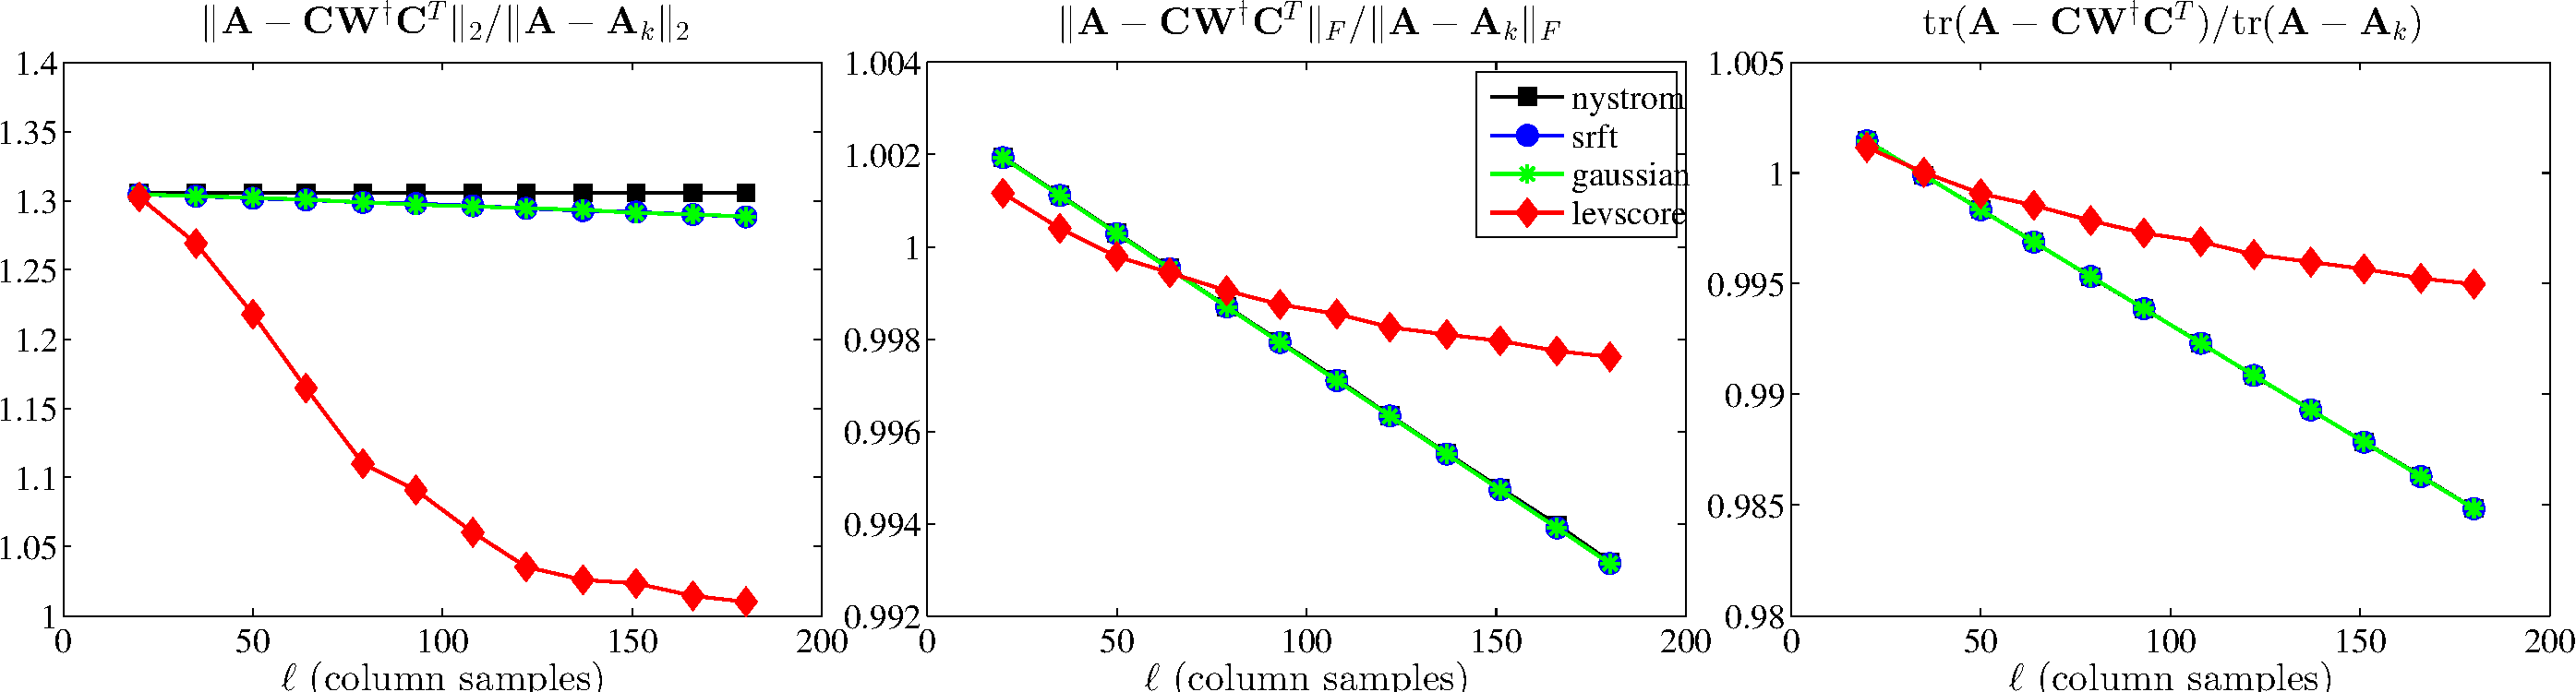
\includegraphics[width=6in, keepaspectratio=true]{figures/ch4/Enronrank20exact-methods-nonfixed-rank-errors}}
 
 \subfigure[Enron, $k = 60$]{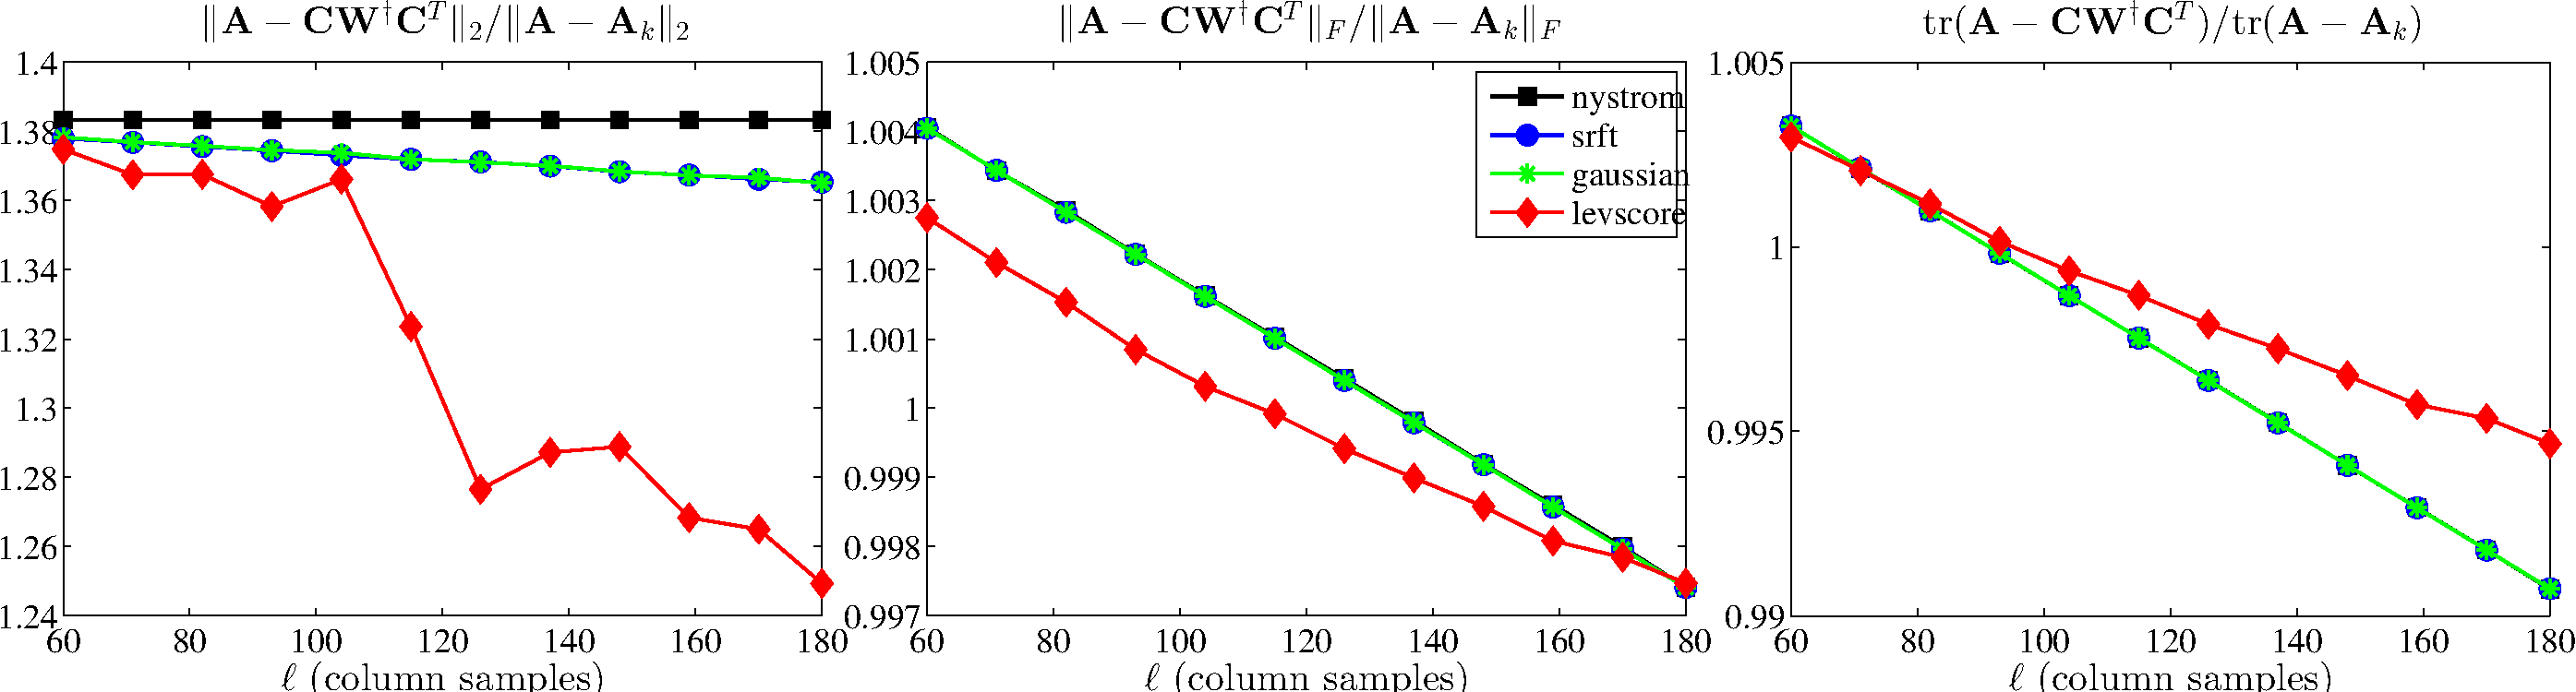
\includegraphics[width=6in, keepaspectratio=true]{figures/ch4/Enronrank60exact-methods-nonfixed-rank-errors}}
 
 \subfigure[Gnutella, $k = 20$]{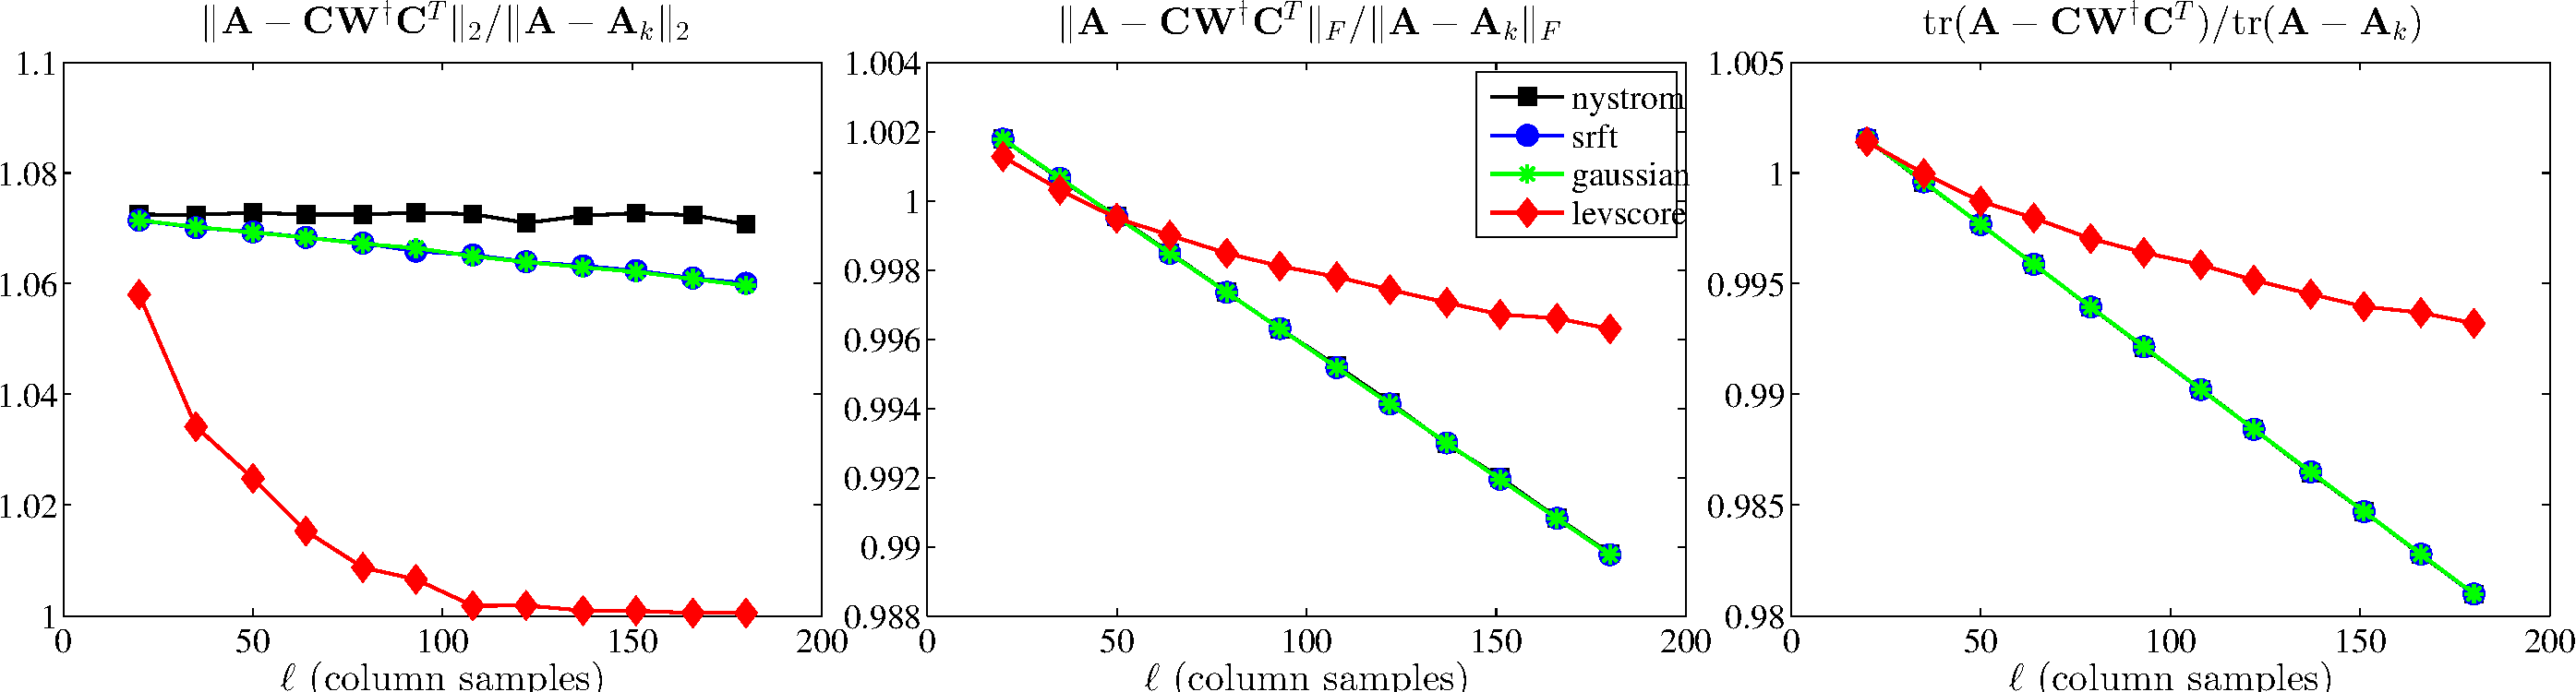
\includegraphics[width=6in, keepaspectratio=true]{figures/ch4/Gnutellarank20exact-methods-nonfixed-rank-errors}}
 
 \subfigure[Gnutella, $k = 60$]{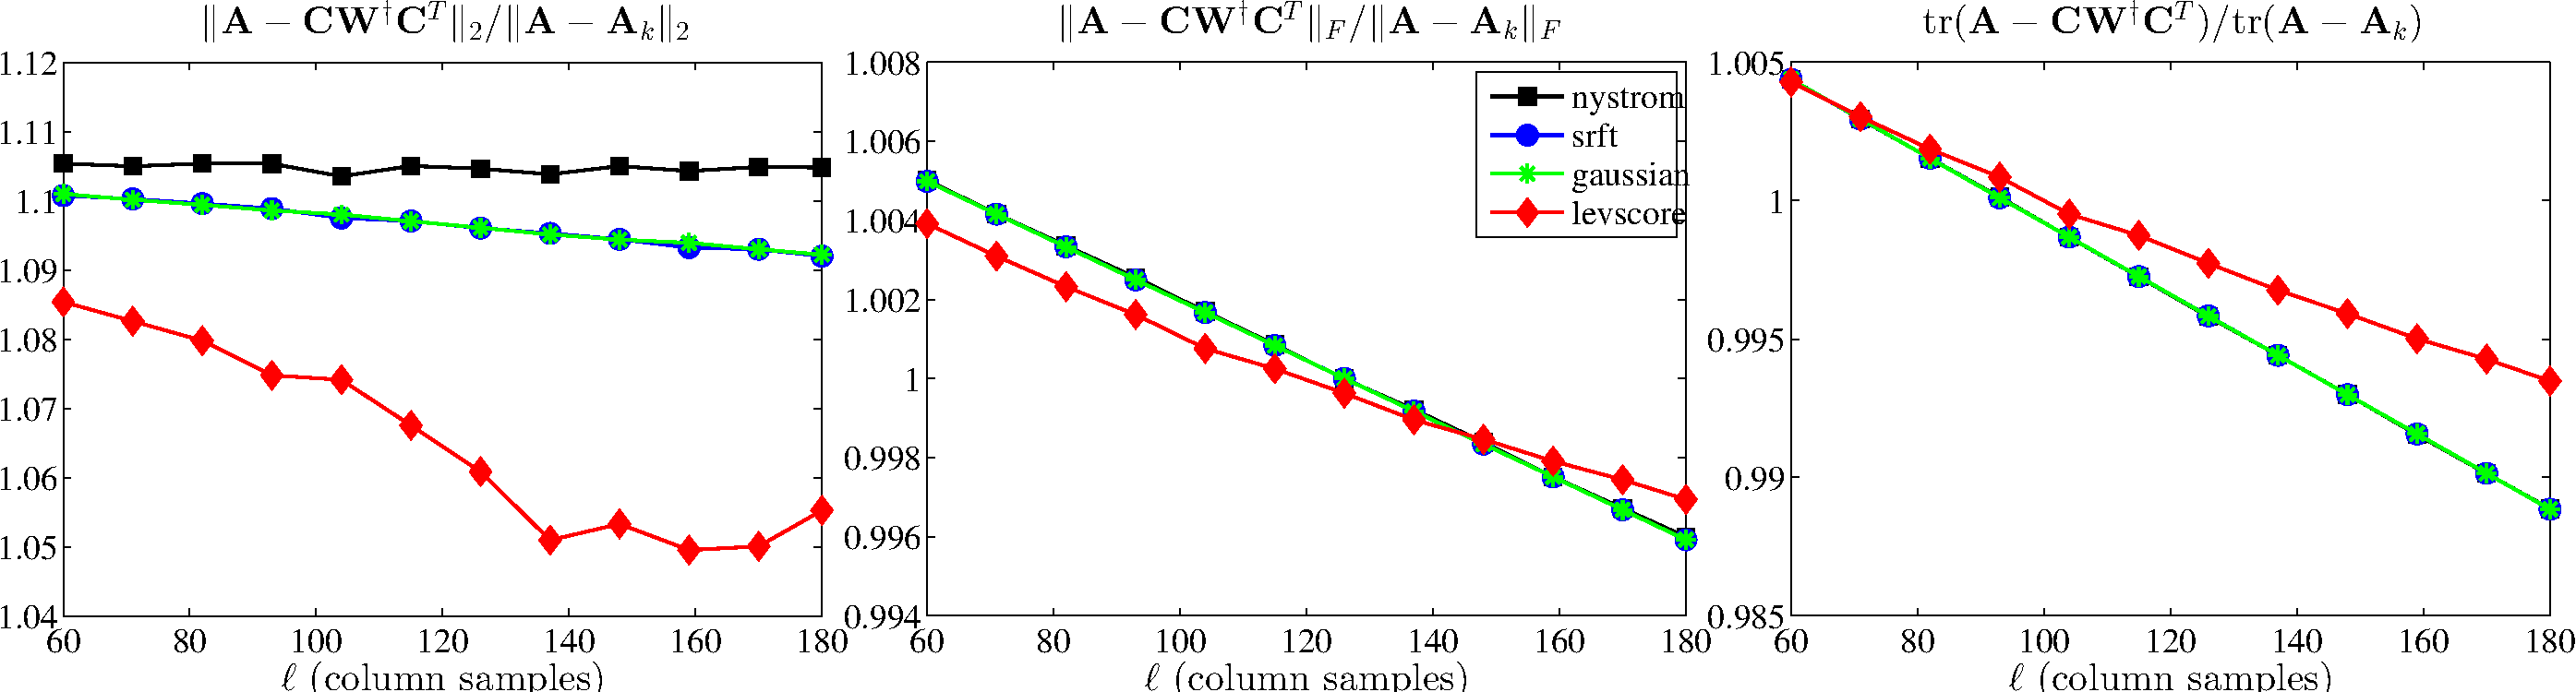
\includegraphics[width=6in, keepaspectratio=true]{figures/ch4/Gnutellarank60exact-methods-nonfixed-rank-errors}}
\caption[Relative errors of non-rank-restricted SPSD sketches of the Enron and Gnutella Laplacian matrices]{%
{\sc Relative errors of non-rank-restricted SPSD sketches of the Enron and Gnutella Laplacian matrices.}
 The relative spectral, Frobenius, and trace-norm errors~\eqref{ch4:eqn:relerr1} of several
 non-rank-restricted SPSD sketches, as a function of the number of columns samples $\ell$, 
 for the Enron and Gnutella Laplacian matrices, with two choices of the rank parameter $k$. }%
 \label{ch4:fig:laplacian-exact-errors-2a}
\end{figure}

\begin{figure}[htp]
 \centering
 \subfigure[GR, $k = 20$]{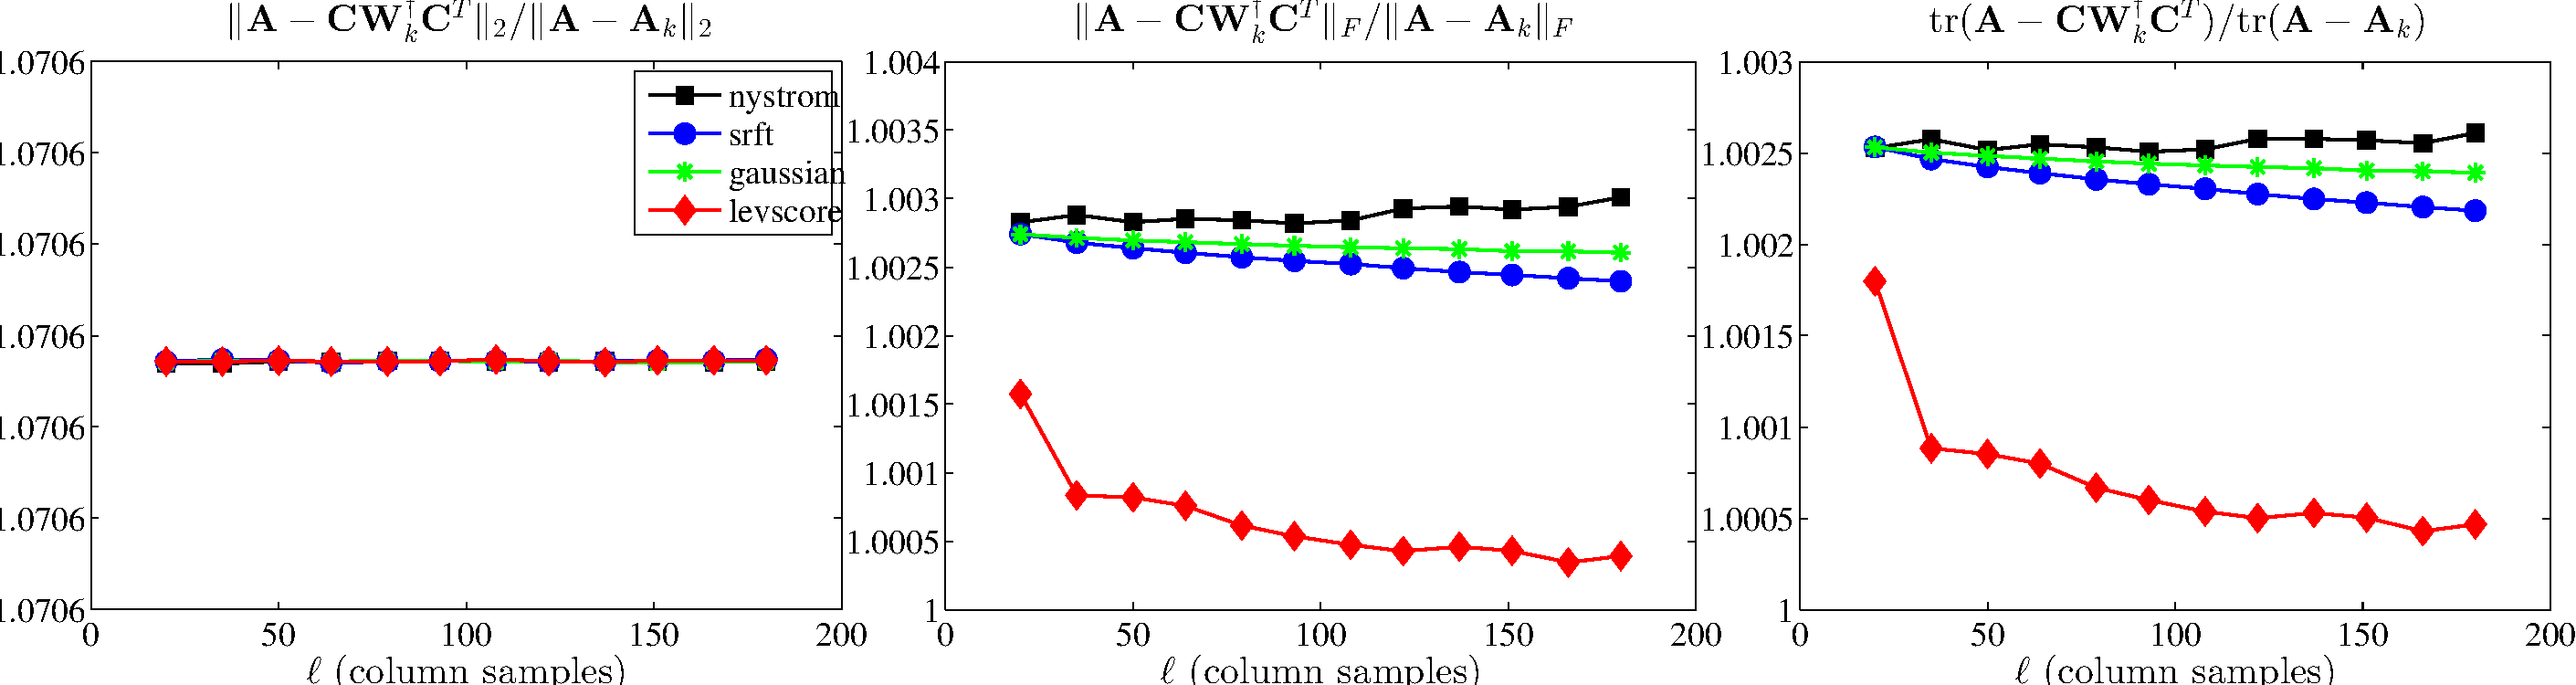
\includegraphics[width=6in, keepaspectratio=true]{figures/ch4/GRrank20exact-methods-fixed-rank-errors}}
 
 \subfigure[GR, $k = 60$]{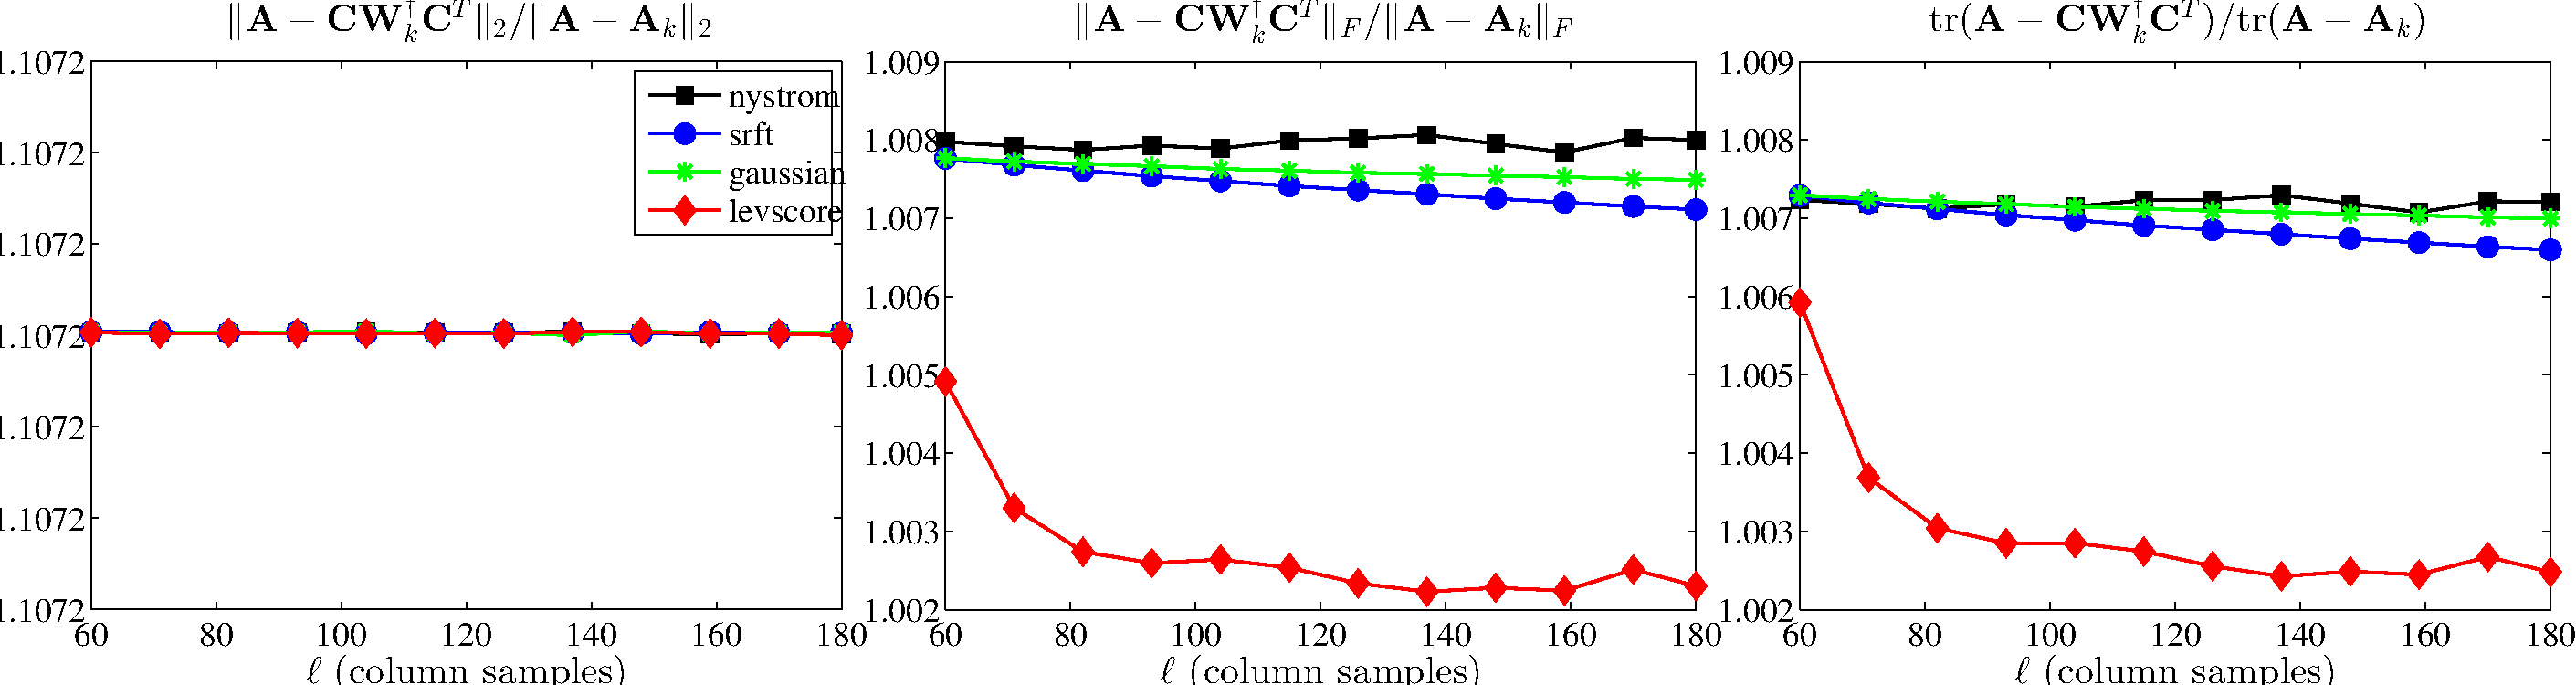
\includegraphics[width=6in, keepaspectratio=true]{figures/ch4/GRrank60exact-methods-fixed-rank-errors}}
 
 \subfigure[HEP, $k = 20$]{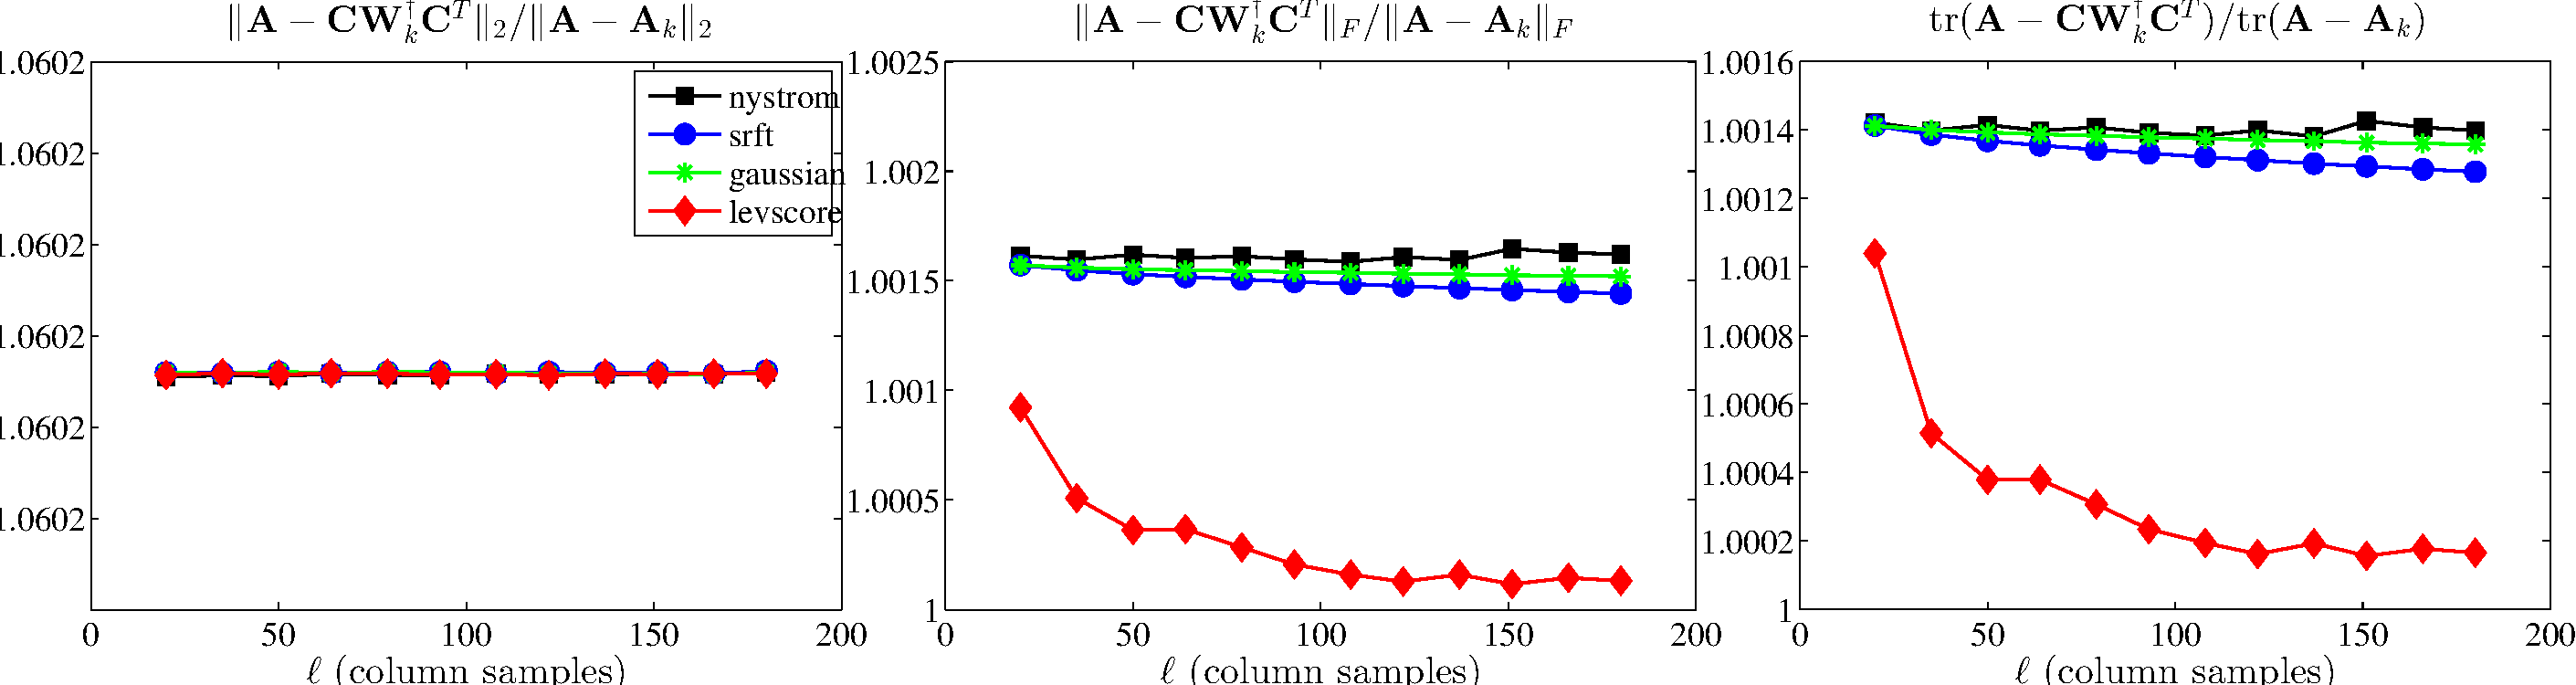
\includegraphics[width=6in, keepaspectratio=true]{figures/ch4/HEPrank20exact-methods-fixed-rank-errors}}
 
 \subfigure[HEP, $k = 60$]{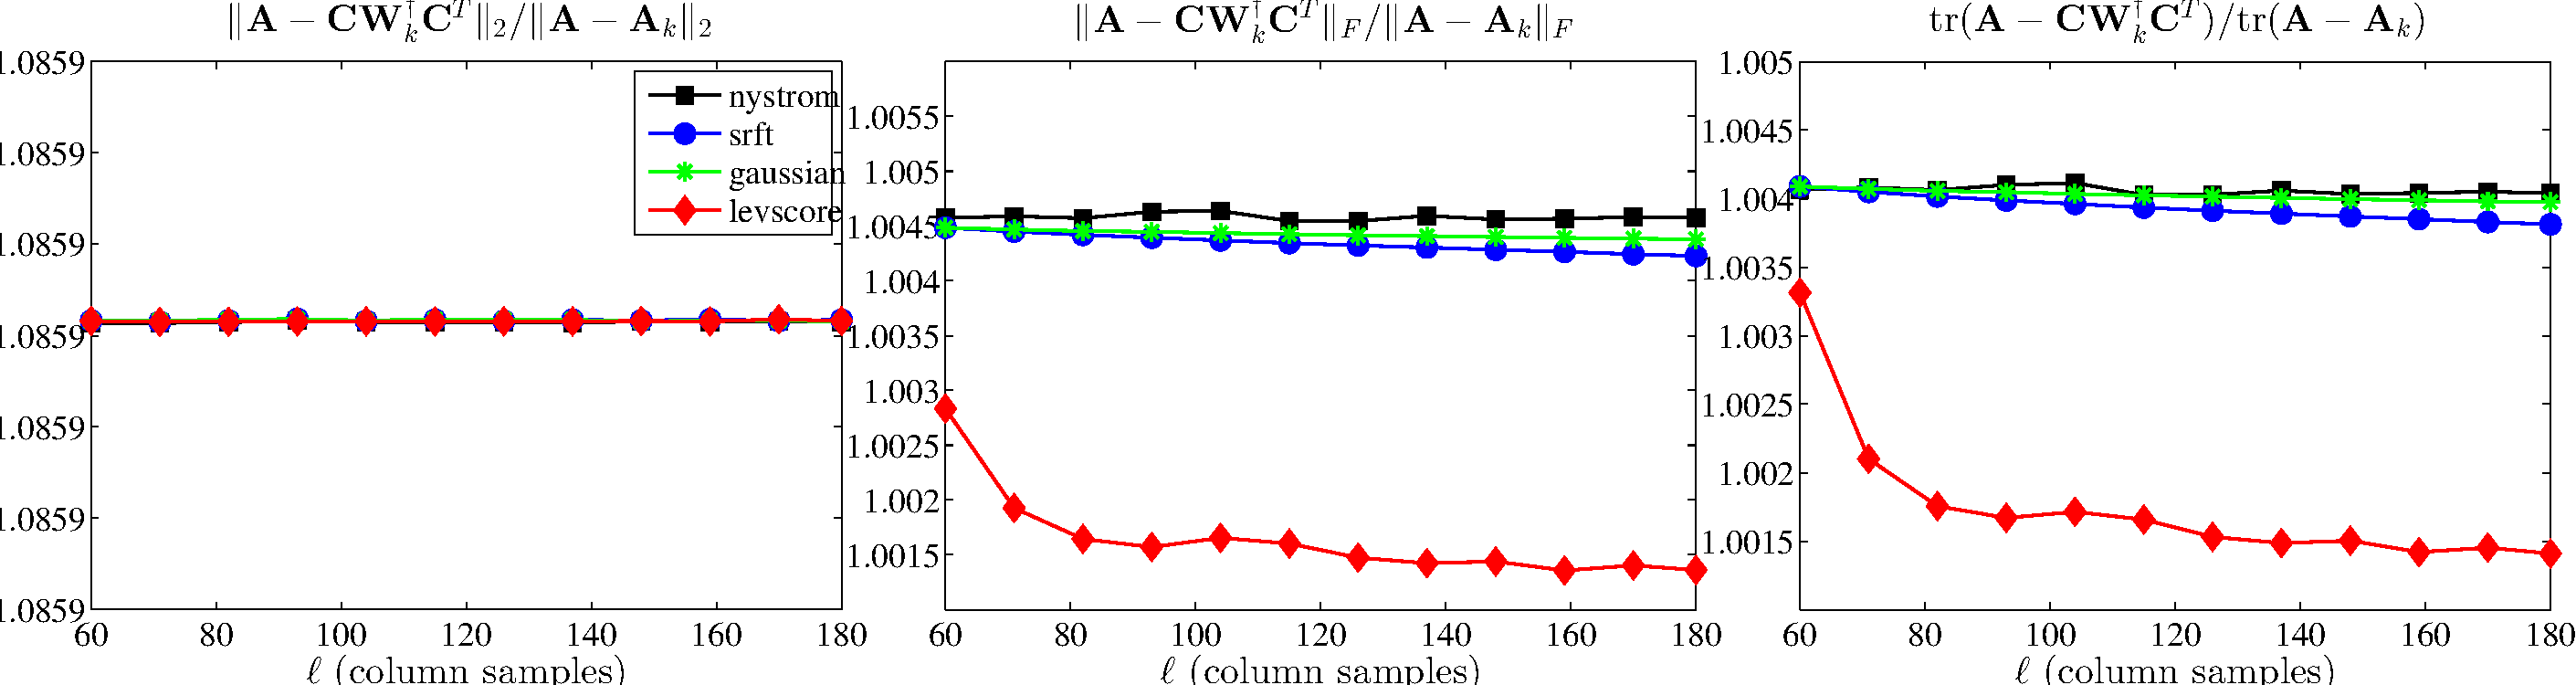
\includegraphics[width=6in, keepaspectratio=true]{figures/ch4/HEPrank60exact-methods-fixed-rank-errors}}
 \caption[Relative errors of rank-restricted SPSD sketches of the GR and HEP Laplacian matrices]{%
 {\sc Relative errors of rank-restricted SPSD sketches of the GR and HEP Laplacian matrices.}
 The relative spectral, Frobenius, and trace-norm errors~\eqref{ch4:eqn:relerr2} of several rank-restricted
 SPSD sketches, as a function of the number of columns samples $\ell$, 
 for the GR and HEP Laplacian matrices, with two choices of the rank parameter $k$.}%
 \label{ch4:fig:laplacian-exact-errors-1b}
\end{figure}

\begin{figure}[htp]
 \centering
 \subfigure[Enron, $k = 20$]{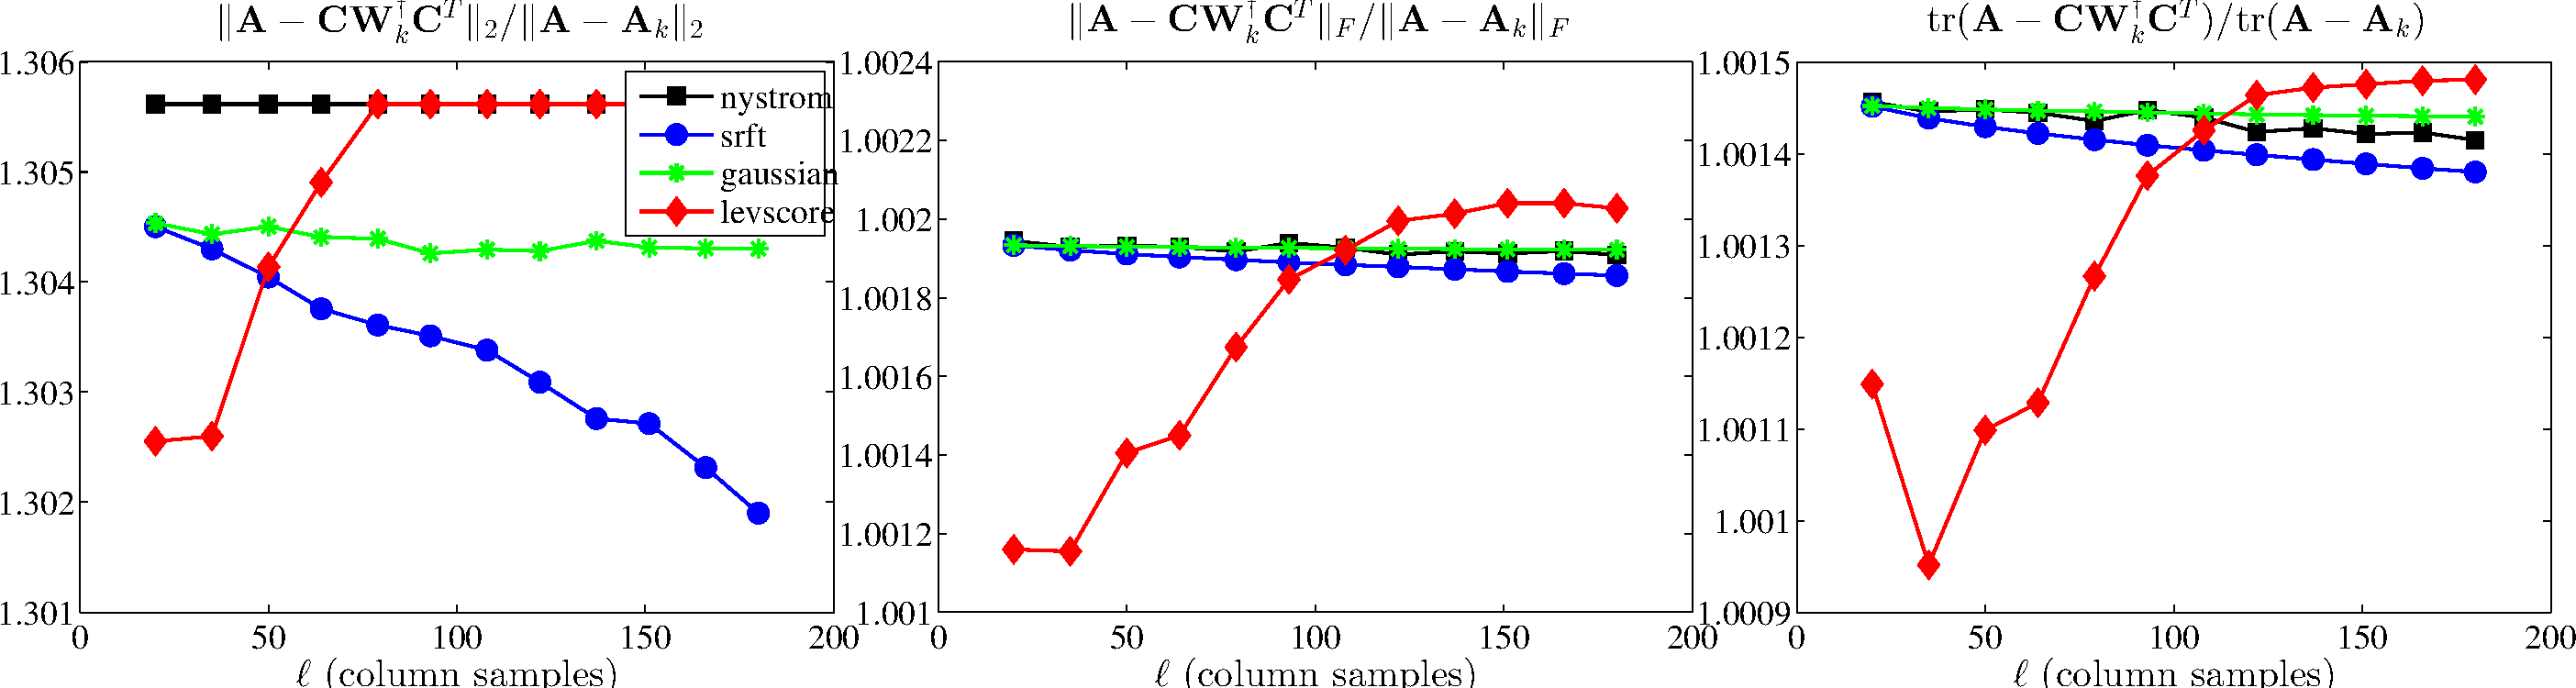
\includegraphics[width=6in, keepaspectratio=true]{figures/ch4/Enronrank20exact-methods-fixed-rank-errors}}
 
 \subfigure[Enron, $k = 60$]{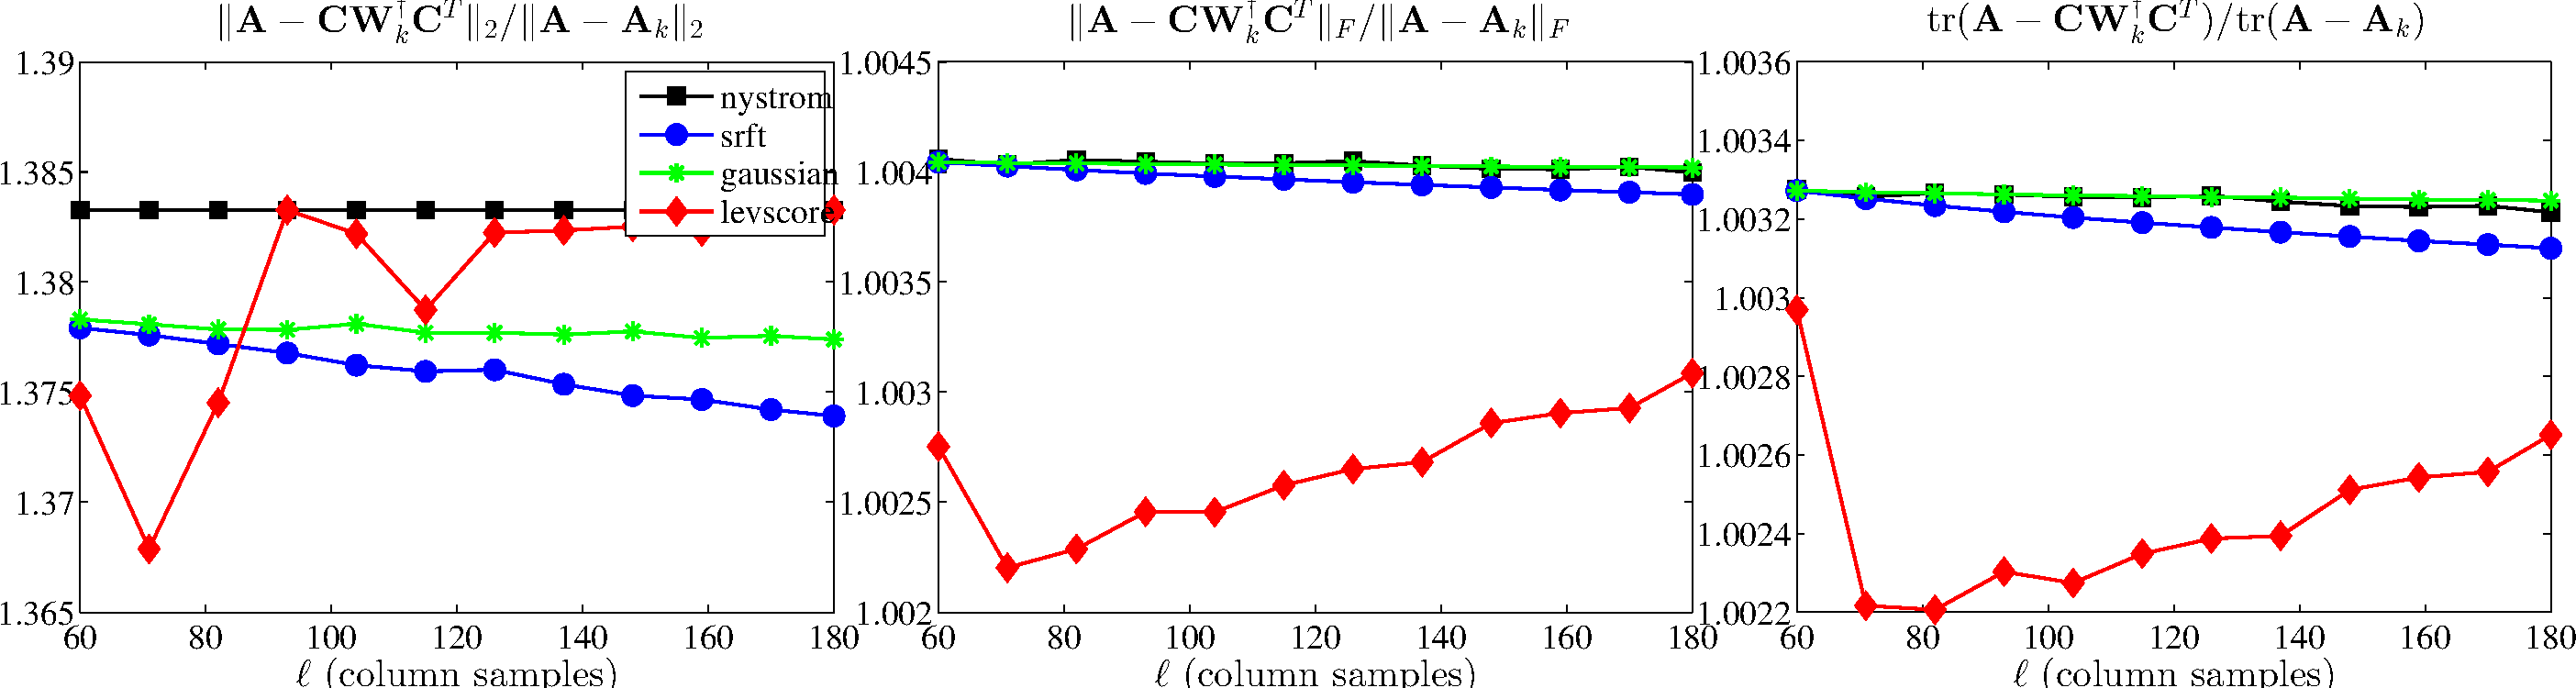
\includegraphics[width=6in, keepaspectratio=true]{figures/ch4/Enronrank60exact-methods-fixed-rank-errors}}
 
 \subfigure[Gnutella, $k = 20$]{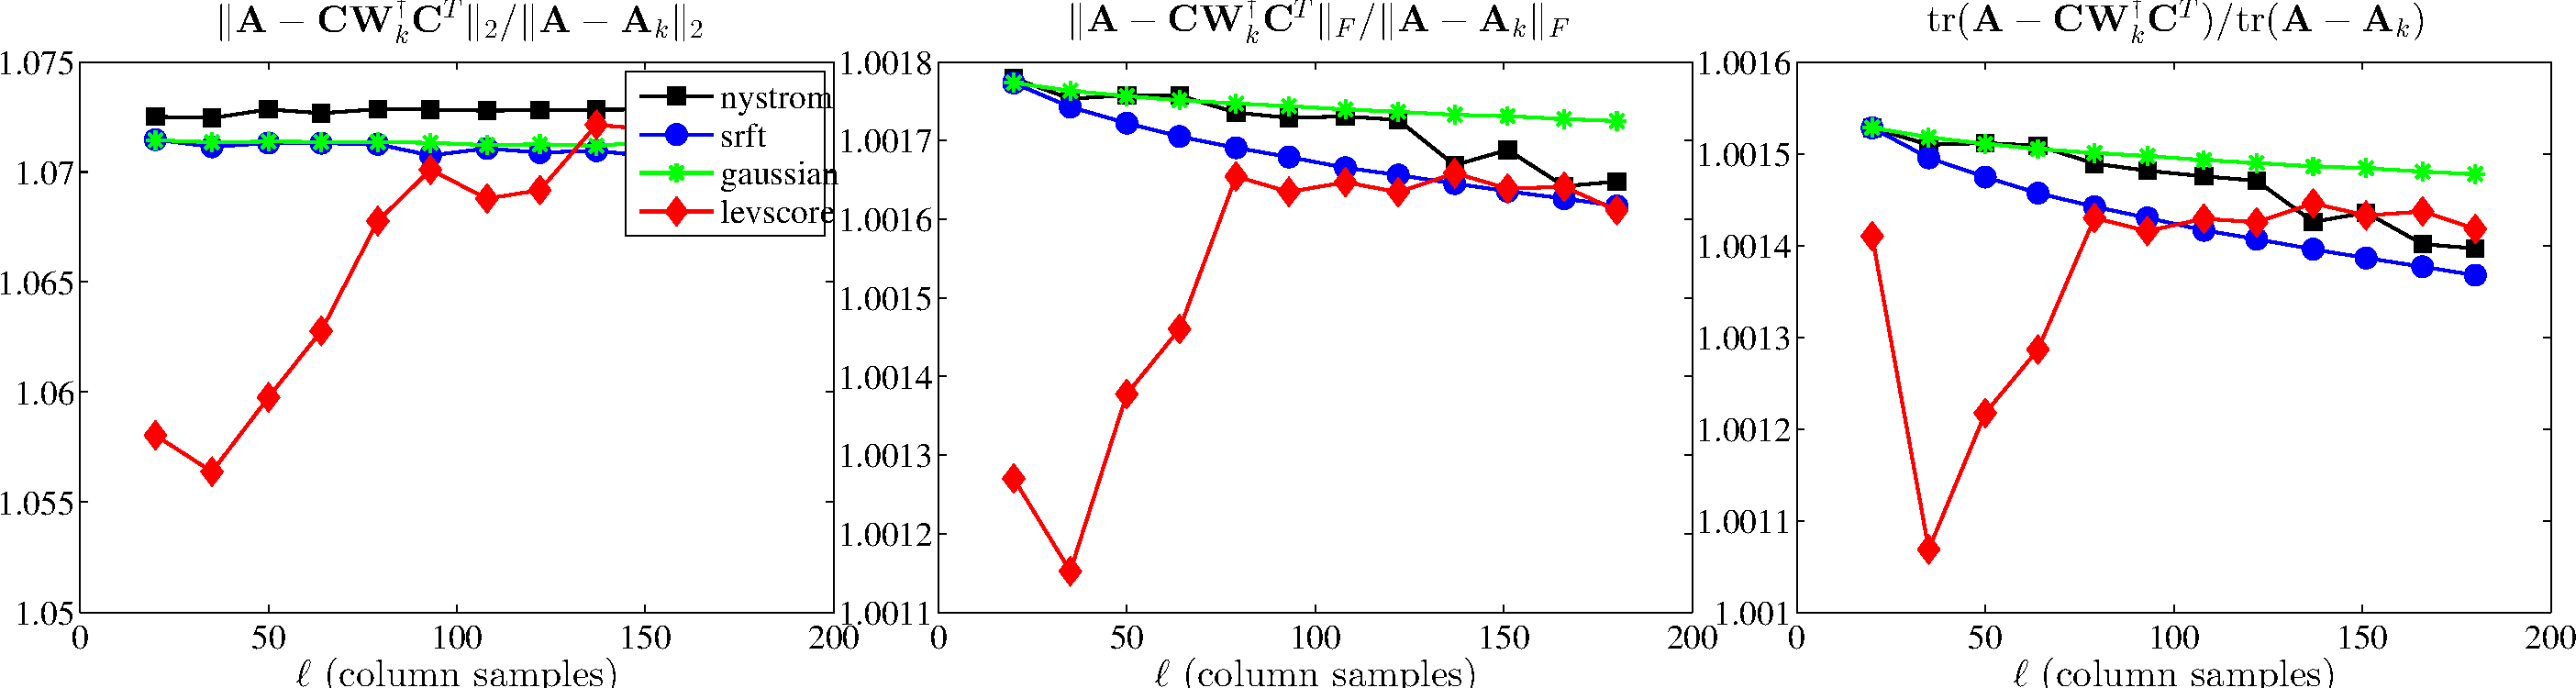
\includegraphics[width=6in, keepaspectratio=true]{figures/ch4/Gnutellarank20exact-methods-fixed-rank-errors}}
 
 \subfigure[Gnutella, $k = 60$]{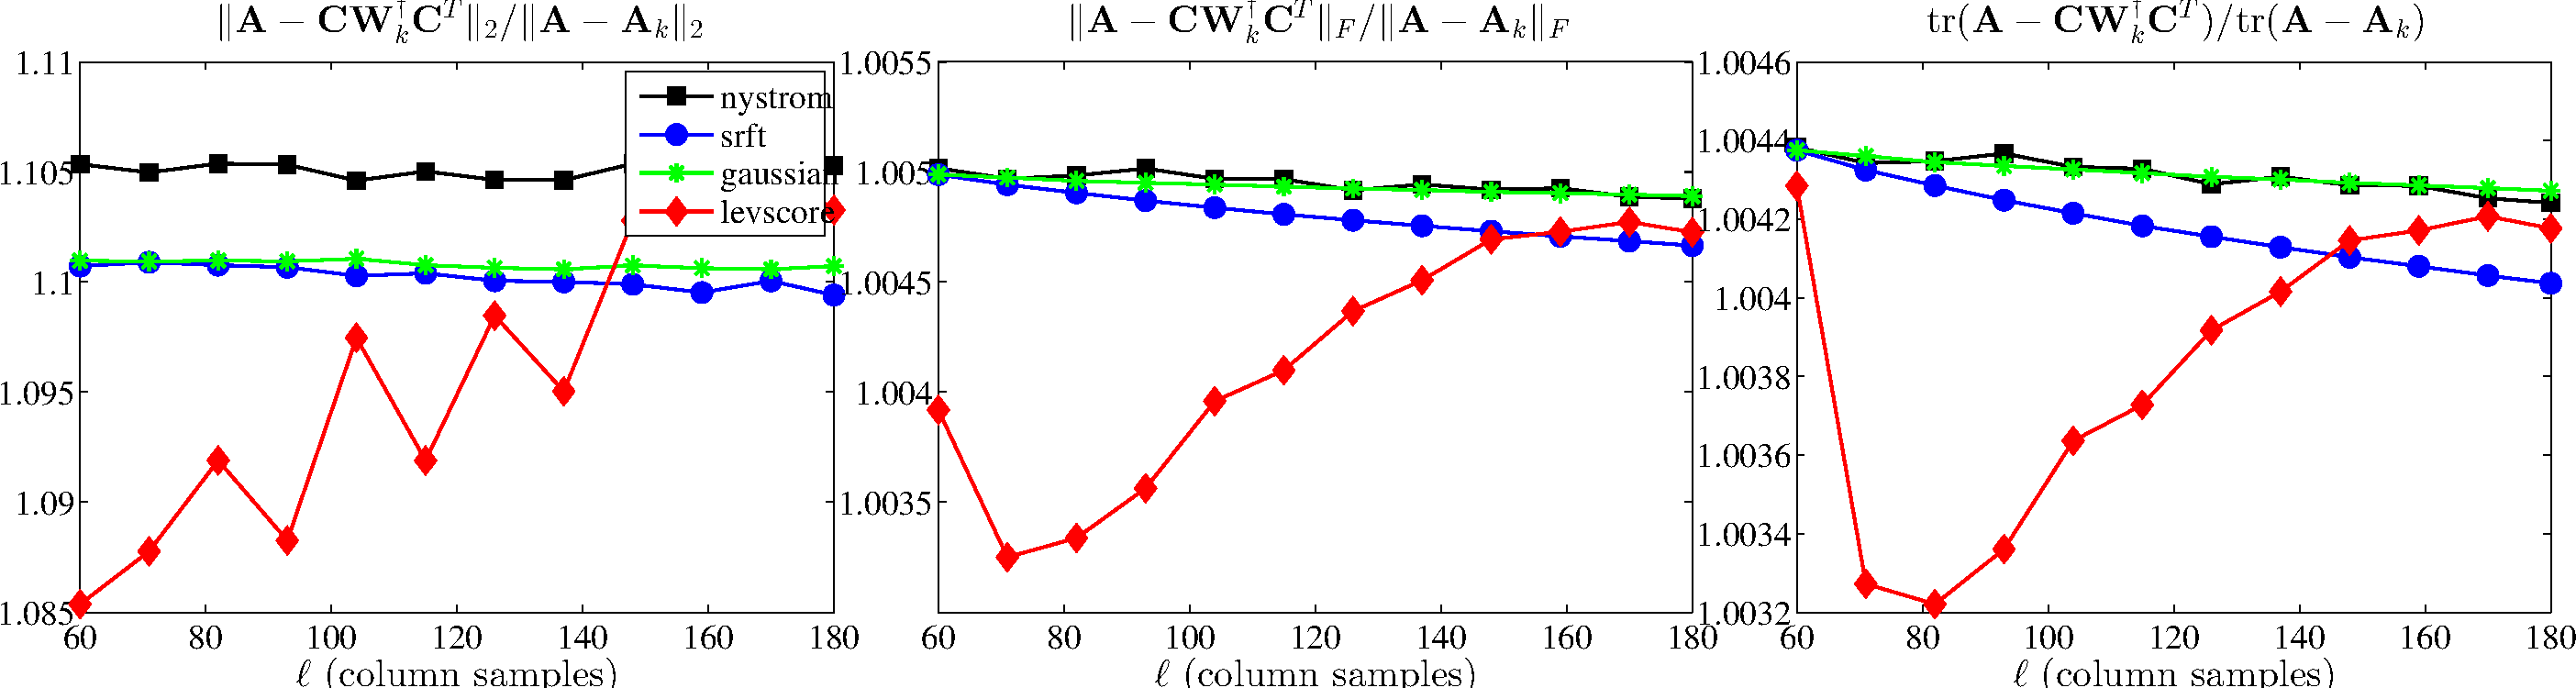
\includegraphics[width=6in, keepaspectratio=true]{figures/ch4/Gnutellarank60exact-methods-fixed-rank-errors}}
 \caption[Relative errors of rank-restricted SPSD sketches of the Enron and Gnutella Laplacian matrices]{%
 {\sc Relative errors of rank-restricted SPSD sketches of the Enron and Gnutella Laplacian matrices.}
 The relative spectral, Frobenius, and trace-norm errors~\eqref{ch4:eqn:relerr2} of several rank-restricted
 SPSD sketches, as a function of the number of columns samples $\ell$, 
 for the Enron and Gnutella Laplacian matrices, with two choices of the rank parameter $k$.}%
 \label{ch4:fig:laplacian-exact-errors-2b}
\end{figure}

Figures~\ref{ch4:fig:laplacian-exact-errors-1a}--\ref{ch4:fig:laplacian-exact-errors-2b} 
show the reconstruction error results for sampling and mixture methods 
applied to several normalized graph Laplacians.
Figures~\ref{ch4:fig:laplacian-exact-errors-1a} and~\ref{ch4:fig:laplacian-exact-errors-1b} 
show GR and HEP, each for two values of the rank parameter. The remaining two show
Enron and Gnutella, again each for two values of the 
rank parameter.
The first two figures show the ratios of the spectral, Frobenius, and trace-norm approximation 
errors of non-rank-restricted sketches to the optimal rank-$k$ 
approximation errors, as a function of the number of column samples~$\ell.$
The remaining two similarly show the errors of the rank-restricted sketches.

These and subsequent figures contain a lot of information, some of which is
peculiar to the given matrices and some of which is more general.
In light of subsequent discussion, several observations are worth making 
about the results presented in these figures.
\begin{itemize}
\item
All of the SPSD sketches provide quite accurate 
approximations even with only $k$ column samples (or 
in the case of the Gaussian and SRFT mixtures, with only $k$ linear 
combinations of vectors). 
Upon examination, this is partly due to the extreme sparsity and extremely 
slow spectral decay of these matrices which means, as shown in 
Table~\ref{ch4:table:datasets}, that only a small fraction of the (spectral or 
Frobenius or trace) mass is captured by the optimal rank $20$ or $60$ 
approximation. 
Thus although an SPSD sketch constructed from $20$ or $60$ vectors also only 
captures a small portion of the mass of the matrix, the relative error is 
small.  
\item
The scale of the vertical axes is different between different figures and 
subfigures.
This is to highlight properties within a given plot, but it can hide 
several things.
In particular, note that the scale for the spectral norm is generally
larger than for the Frobenius norm, which is generally larger than for the
trace norm, consistent with the size of those norms; and that the scale is 
larger for higher-rank approximations, e.g. compare GR $k=20$ with 
GR $k=60$, also consistent with the larger amount of mass captured by 
higher-rank approximations.
\item
Both the non-rank-restricted and rank-restricted results are the same for 
$\ell=k$.
For $\ell > k$, the non-rank-restricted errors tend to decrease (or 
at least not increase, as for GR and HEP the spectral norm error is flat as 
a function of $\ell$), which is intuitive.
While the rank-restricted errors also tend to decrease for $\ell > k$, 
the decrease is much less (since the rank-restricted plots are bounded below 
by unity) and the behavior is much more complicated as a function of 
increasing $\ell$.
\item
The horizontal axes range from $k$ to $9k$ for the $k=20$ plots and to $3k$ for the 
$k=60$ plots.
As a practical matter, choosing $\ell$ between $k$ and (say) $2k$ or $3k$ is 
probably of greatest interest.
In this regime, there is an interesting tradeoff for the non-rank-restricted
plots: for moderately large values of $\ell$ in this regime, the error for 
leverage-based sampling is moderately better than for uniform sampling or 
random mixtures, while if one chooses $\ell$ to be much larger then the 
improvements from leverage-based sampling saturate and the uniform sampling 
and random mixture methods are better.
This is most obvious in the Frobenius-norm plots, although it is also seen in
the trace norm plots, and it suggests that some combination of leverage-based
sampling and uniform sampling might be best.
\item
For the rank-restricted plots, in some cases, e.g., with GR and HEP, 
the errors for leverage-based sampling are much better than for the other 
methods and quickly improve with increasing $\ell$ until they saturate; 
while in other cases, e.g., with Enron and Gnutella, the errors for
leverage-based sampling improve quickly and then degrade with increasing 
$\ell$.
Upon examination, the former phenomenon is similar to what was observed in 
the non-rank-restricted case and is due to the strong ``bias'' provided by 
the leverage score importance sampling distribution to the top part of the 
spectrum, allowing the sampling process to focus very quickly on the 
low-rank part of the input matrix.
(In some cases, this is due to the fact that the heterogeneity of 
the leverage score importance sampling distribution means that one is likely 
to choose the same high leverage columns multiple times, rather than 
increasing the accuracy of the extension by adding new columns whose 
leverage scores are lower.) 
The latter phenomenon of degrading error quality as $\ell$ is increased is 
more complex and seems to be due to some sort of ``overfitting'' caused by 
this strong bias and by choosing many more than $k$ columns.  
%% Although we do not completely undersand it, this phenomenon is seen in 
%% several of the examples below.
\item
The behavior of the approximations with respect to the spectral norm is 
quite different from the behavior in the Frobenius and trace norms. 
In the latter, as the number of samples $\ell$ increases, the errors tend to 
decrease, although in an erratic manner for some of the rank-restricted 
plots; while for the former, the errors tend to be much flatter as a function 
of increasing $\ell$ for at least the Gaussian, SRFT, and uniformly column sampled (i.e., Nystr\"om)
sketches.
\end{itemize}
All in all, there seems to be quite complicated behavior for low-rank 
sketches for these Laplacian matrices.
Several of these observations can also be made for subsequent figures; but
in some other cases the (very sparse and not very low rank) structural 
properties of the data are primarily responsible.

\subsubsection{Linear kernels}

\begin{figure}[htp]
 \centering
 \subfigure[Dexter, $k = 8$]{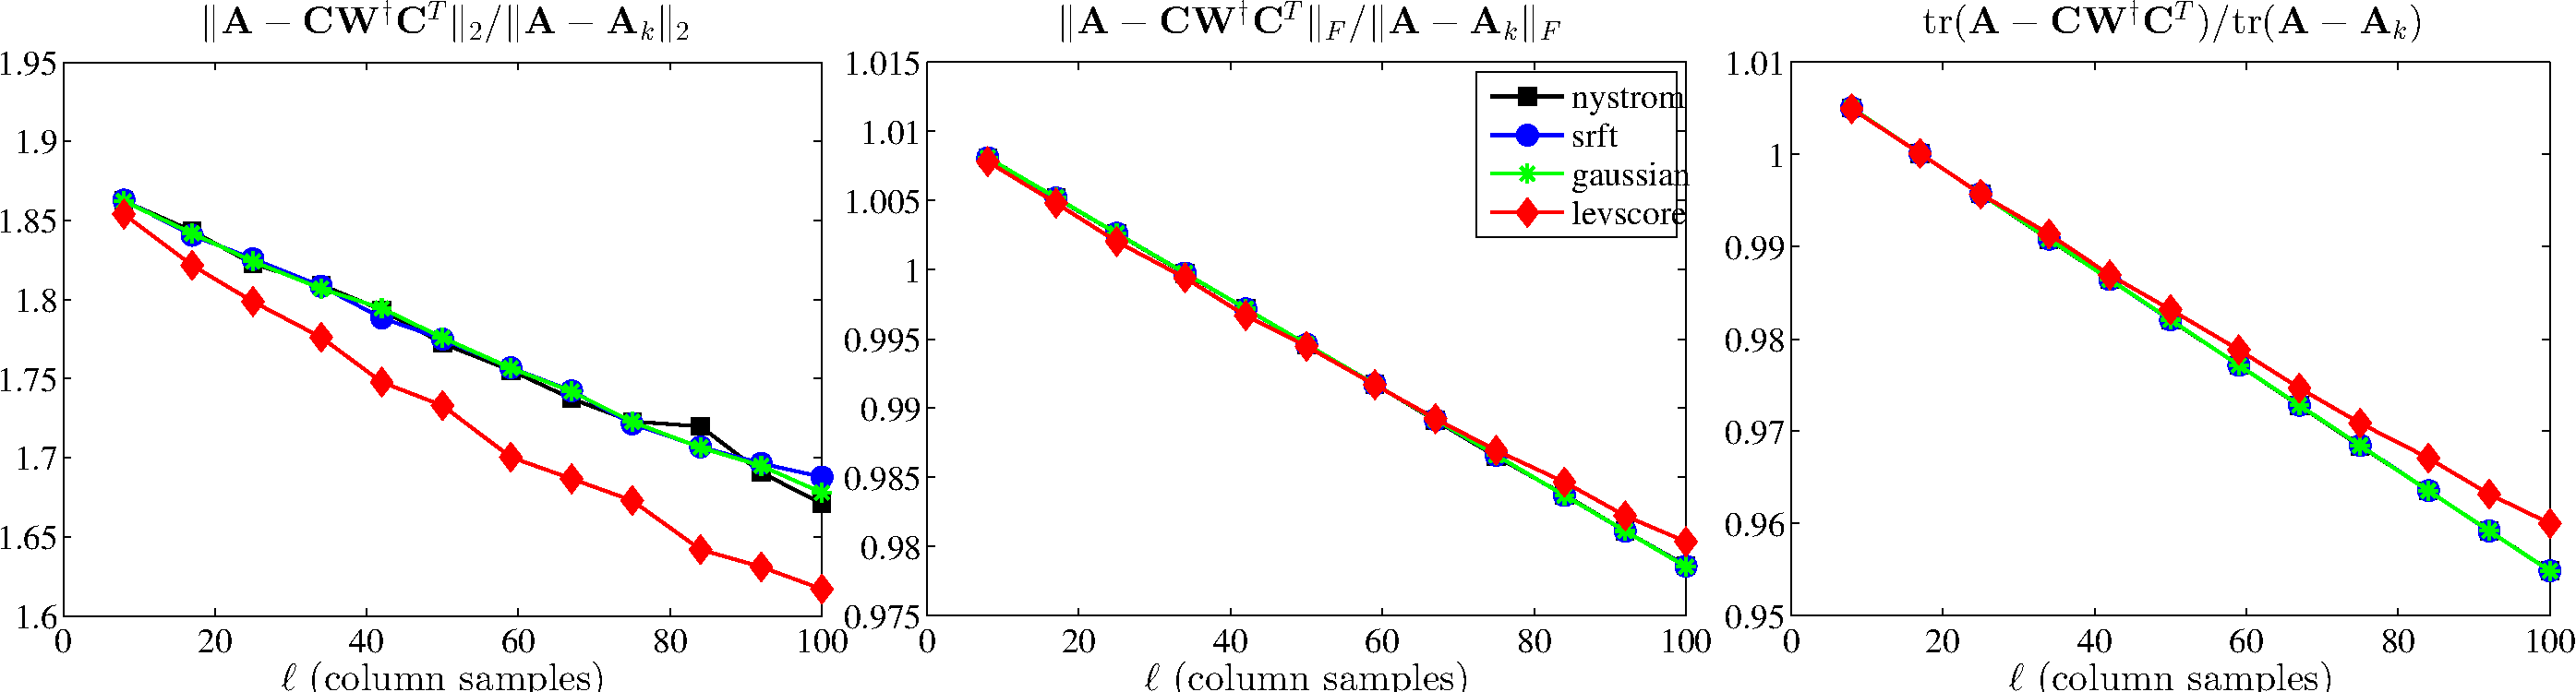
\includegraphics[width=6in, keepaspectratio=true]{figures/ch4/Dexterrank8exact-methods-nonfixed-rank-errors}}
 
 \subfigure[Protein, $k = 10$]{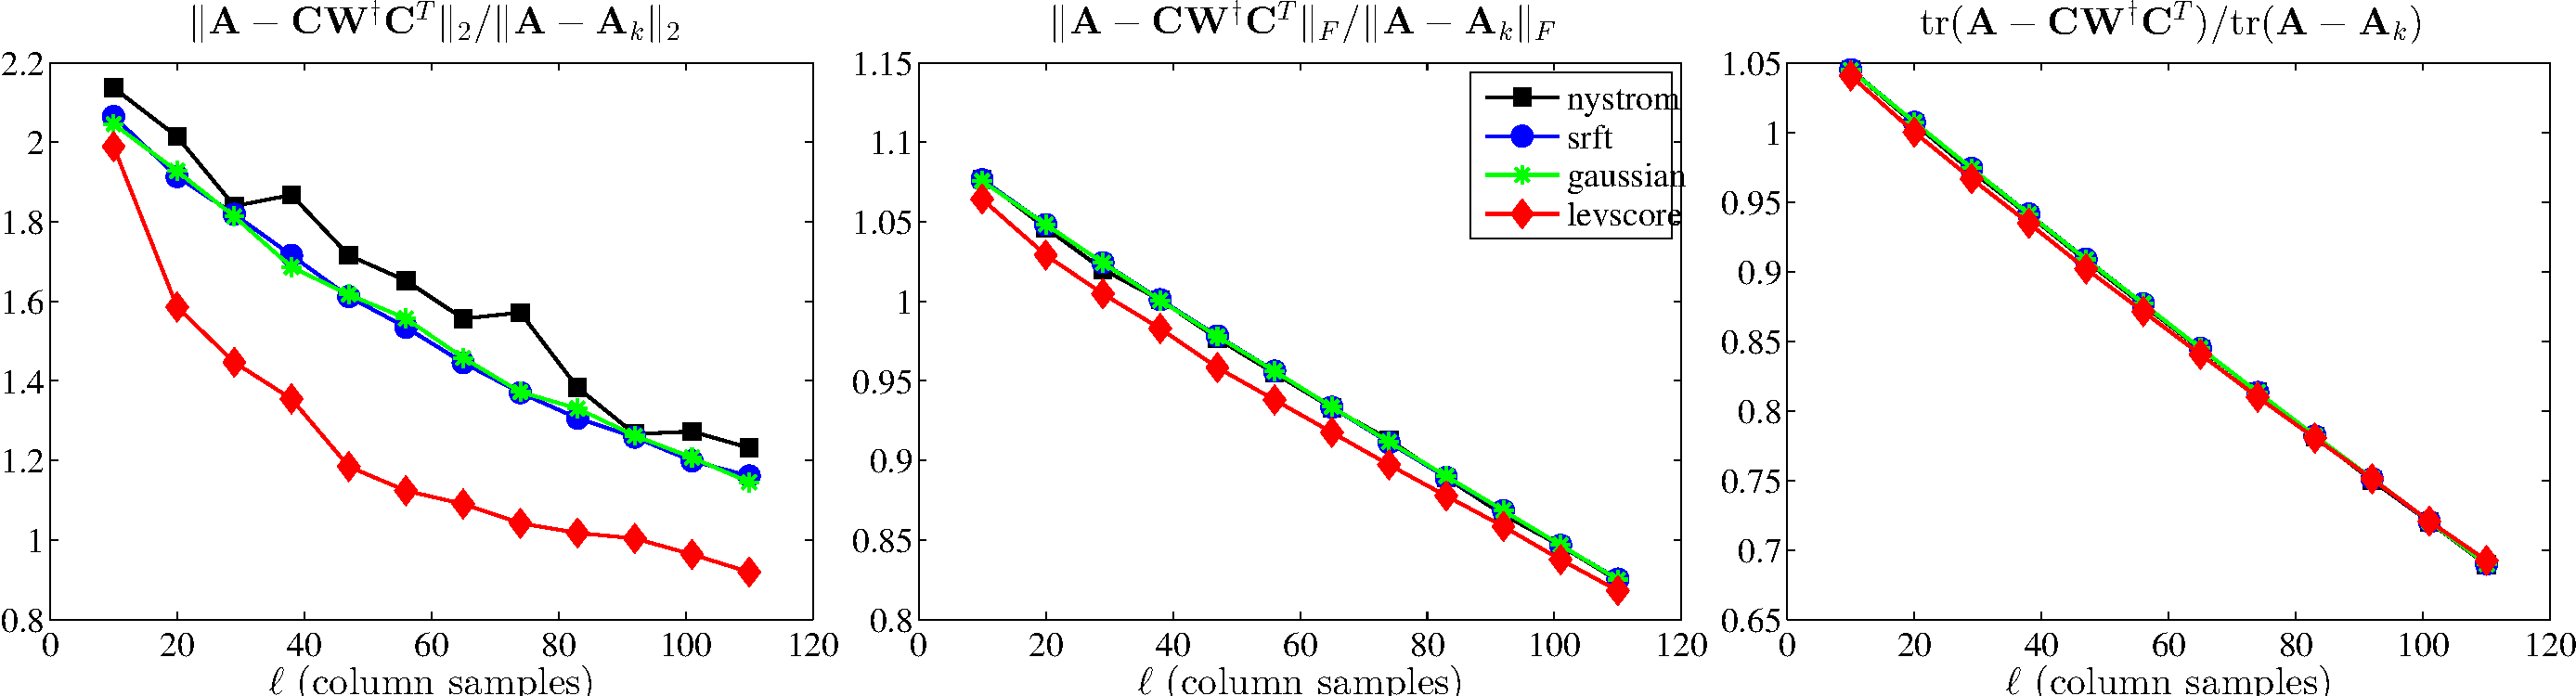
\includegraphics[width=6in, keepaspectratio=true]{figures/ch4/Proteinrank10exact-methods-nonfixed-rank-errors}}
 
 \subfigure[SNPs, $k = 5$]{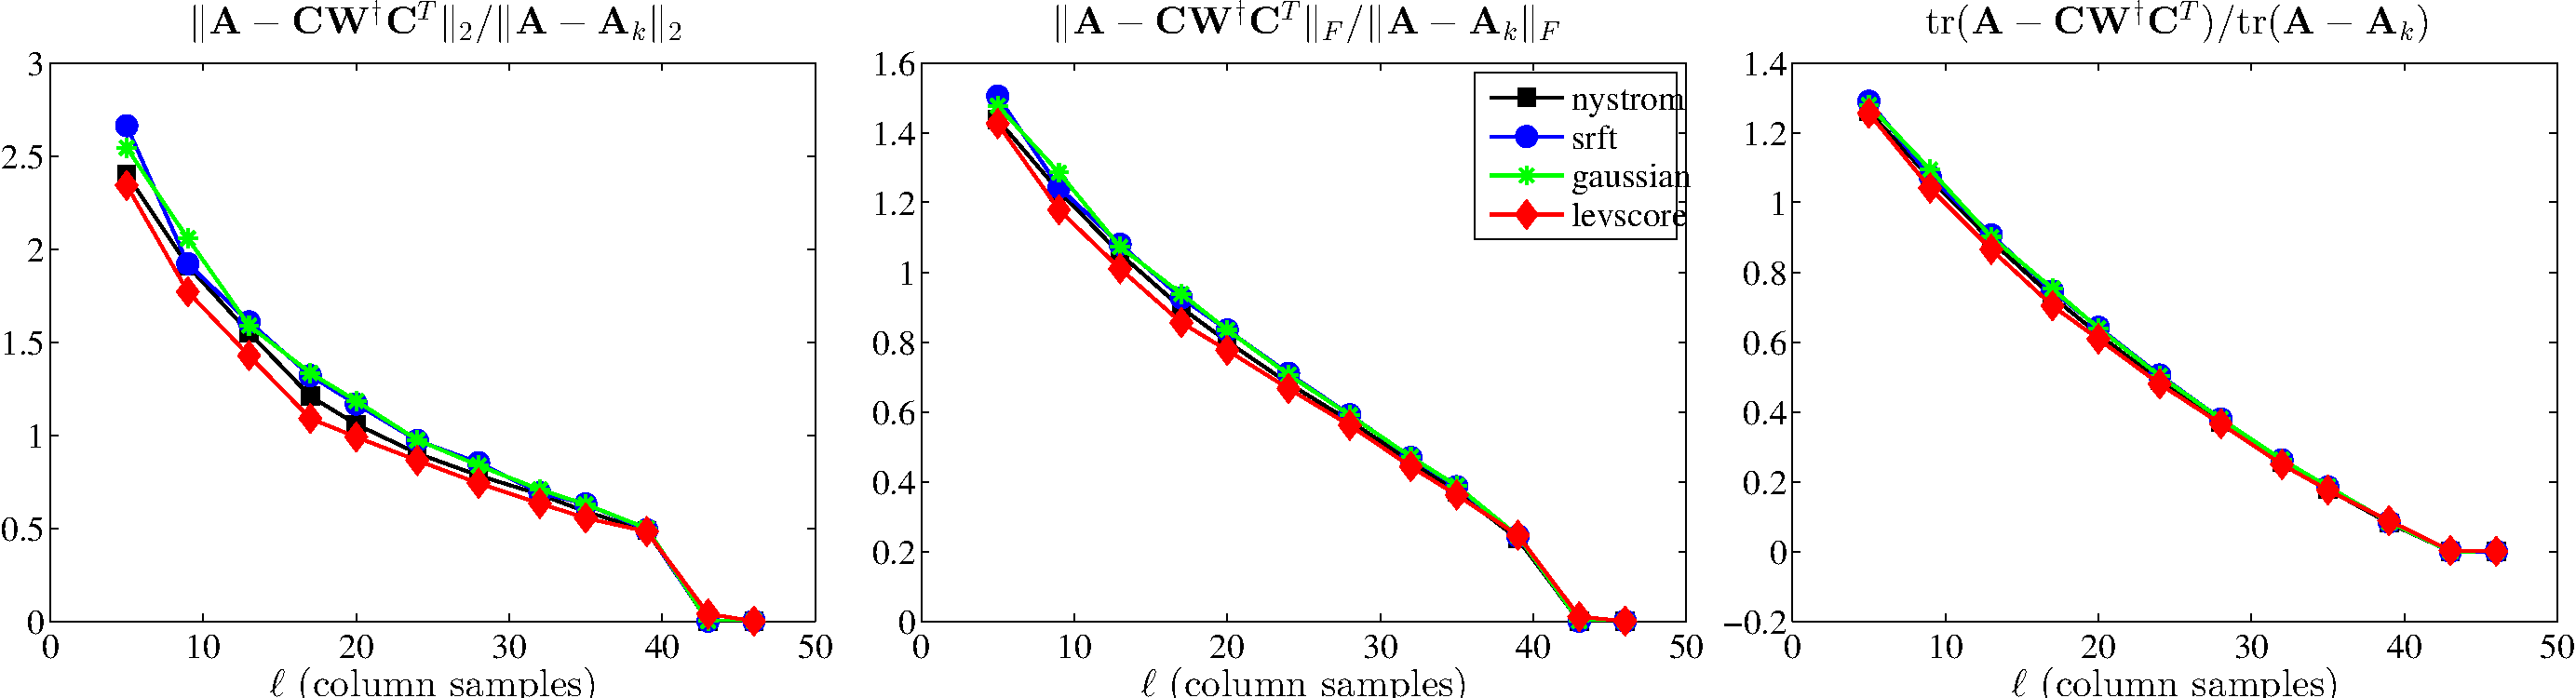
\includegraphics[width=6in, keepaspectratio=true]{figures/ch4/SNPSrank5exact-methods-nonfixed-rank-errors}}
 
 \subfigure[Gisette, $k = 12$]{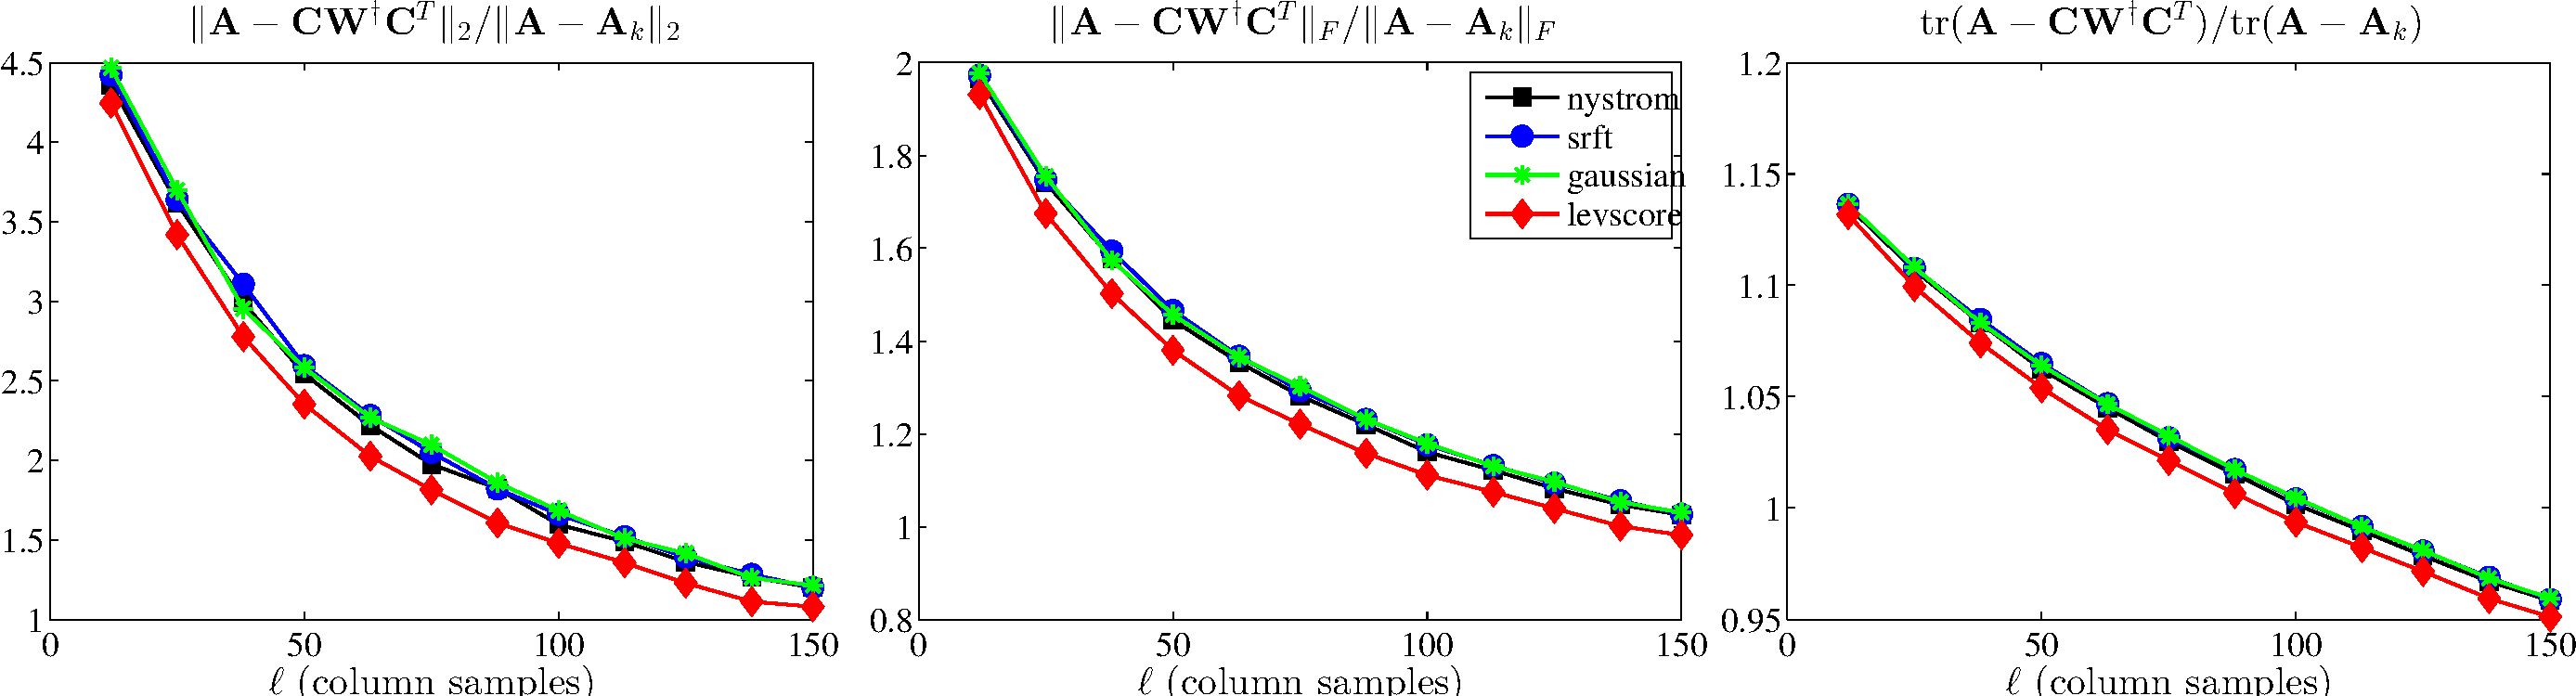
\includegraphics[width=6in, keepaspectratio=true]{figures/ch4/Gisetterank12exact-methods-nonfixed-rank-errors}}
 \caption[Relative errors of non-rank-restricted SPSD sketches of the linear kernel matrices]{%
 {\sc Relative errors of non-rank-restricted SPSD sketches of the linear kernel matrices.}
 The relative spectral, Frobenius, and trace-norm errors~\eqref{ch4:eqn:relerr1} of several non-rank-restricted
 SPSD sketches, as a function of the number of columns samples $\ell$, 
 for the linear kernel matrices.}%
 \label{ch4:fig:linearkernel-exact-errors-a}
\end{figure}

\begin{figure}[htp]
 \centering
 \subfigure[Dexter, $k = 8$]{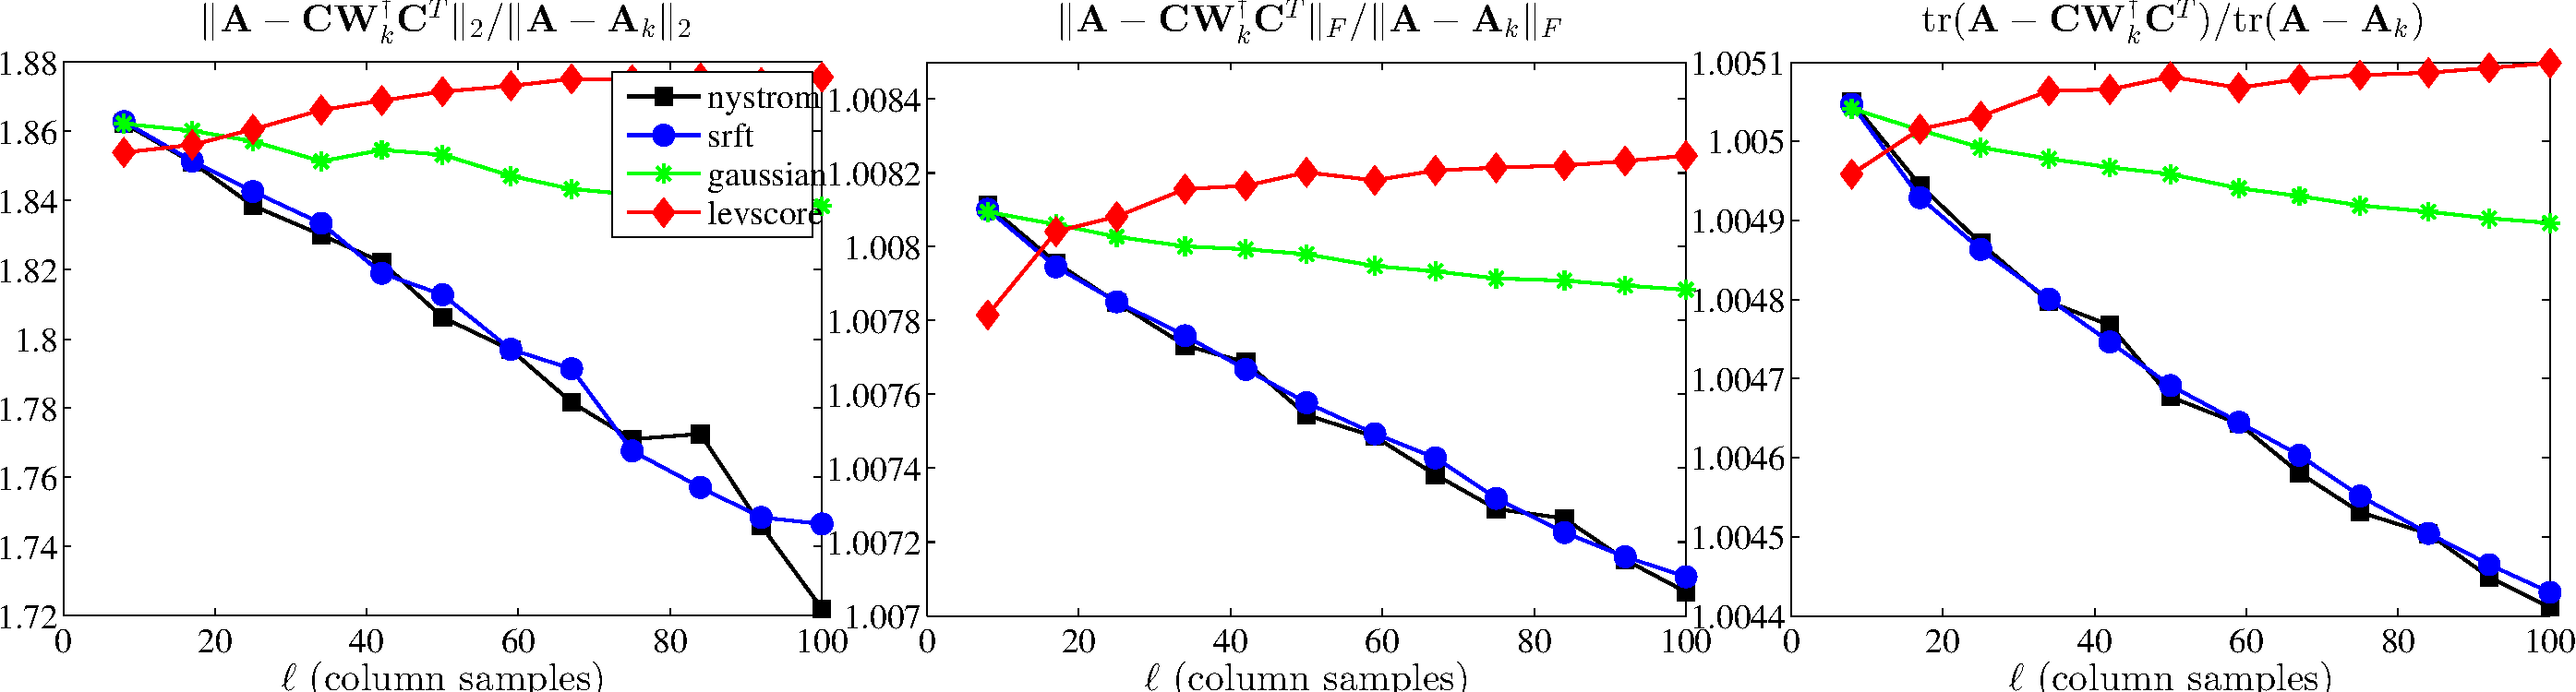
\includegraphics[width=6in, keepaspectratio=true]{figures/ch4/Dexterrank8exact-methods-fixed-rank-errors}}
 
 \subfigure[Protein, $k = 10$]{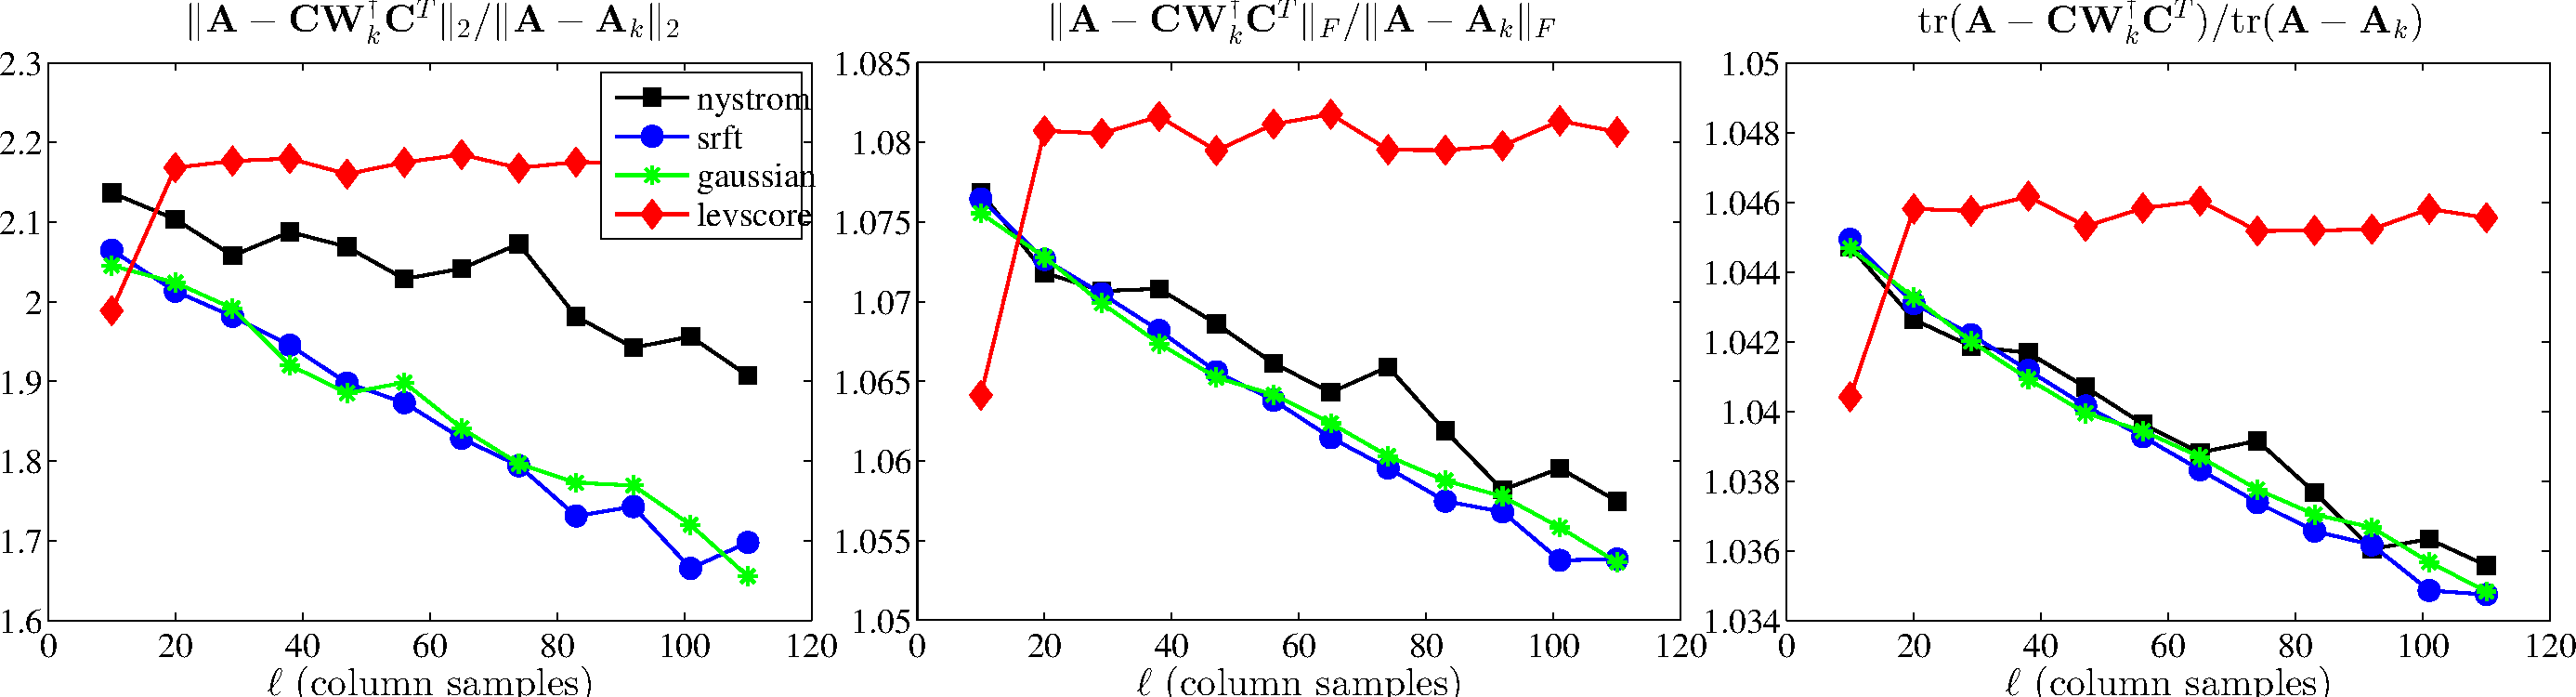
\includegraphics[width=6in, keepaspectratio=true]{figures/ch4/Proteinrank10exact-methods-fixed-rank-errors}}
 
 \subfigure[SNPs, $k = 5$]{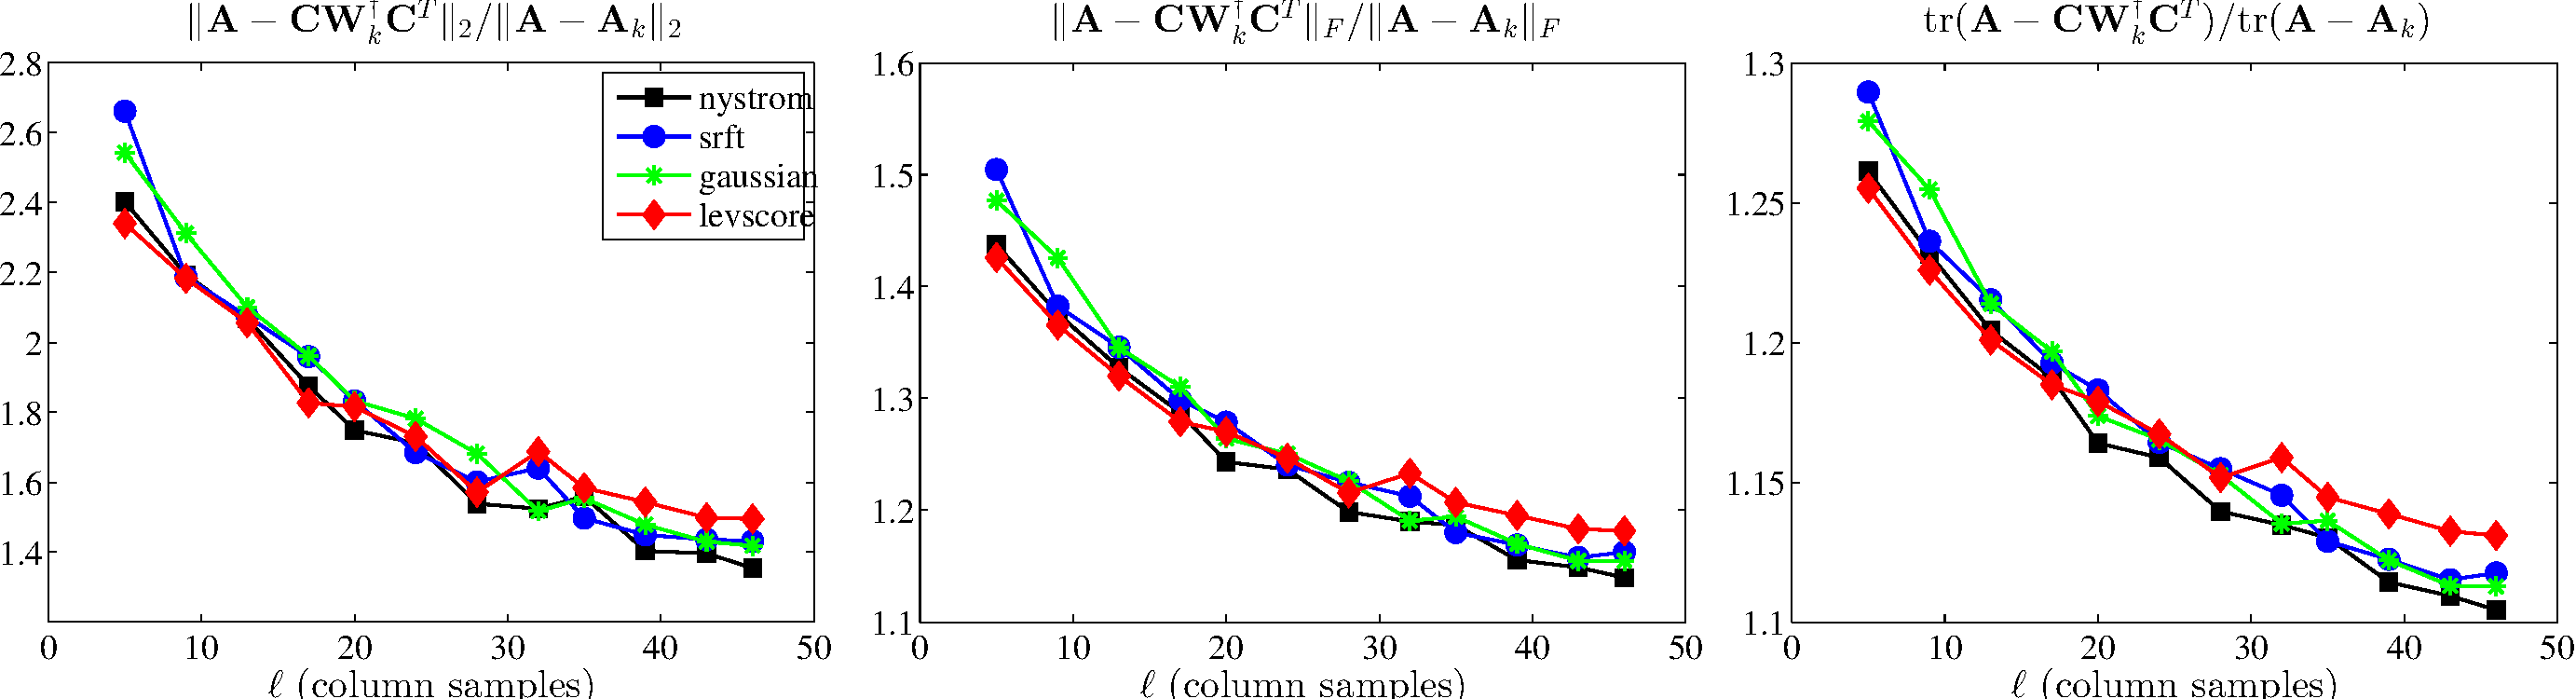
\includegraphics[width=6in, keepaspectratio=true]{figures/ch4/SNPSrank5exact-methods-fixed-rank-errors}}
 
 \subfigure[Gisette, $k = 12$]{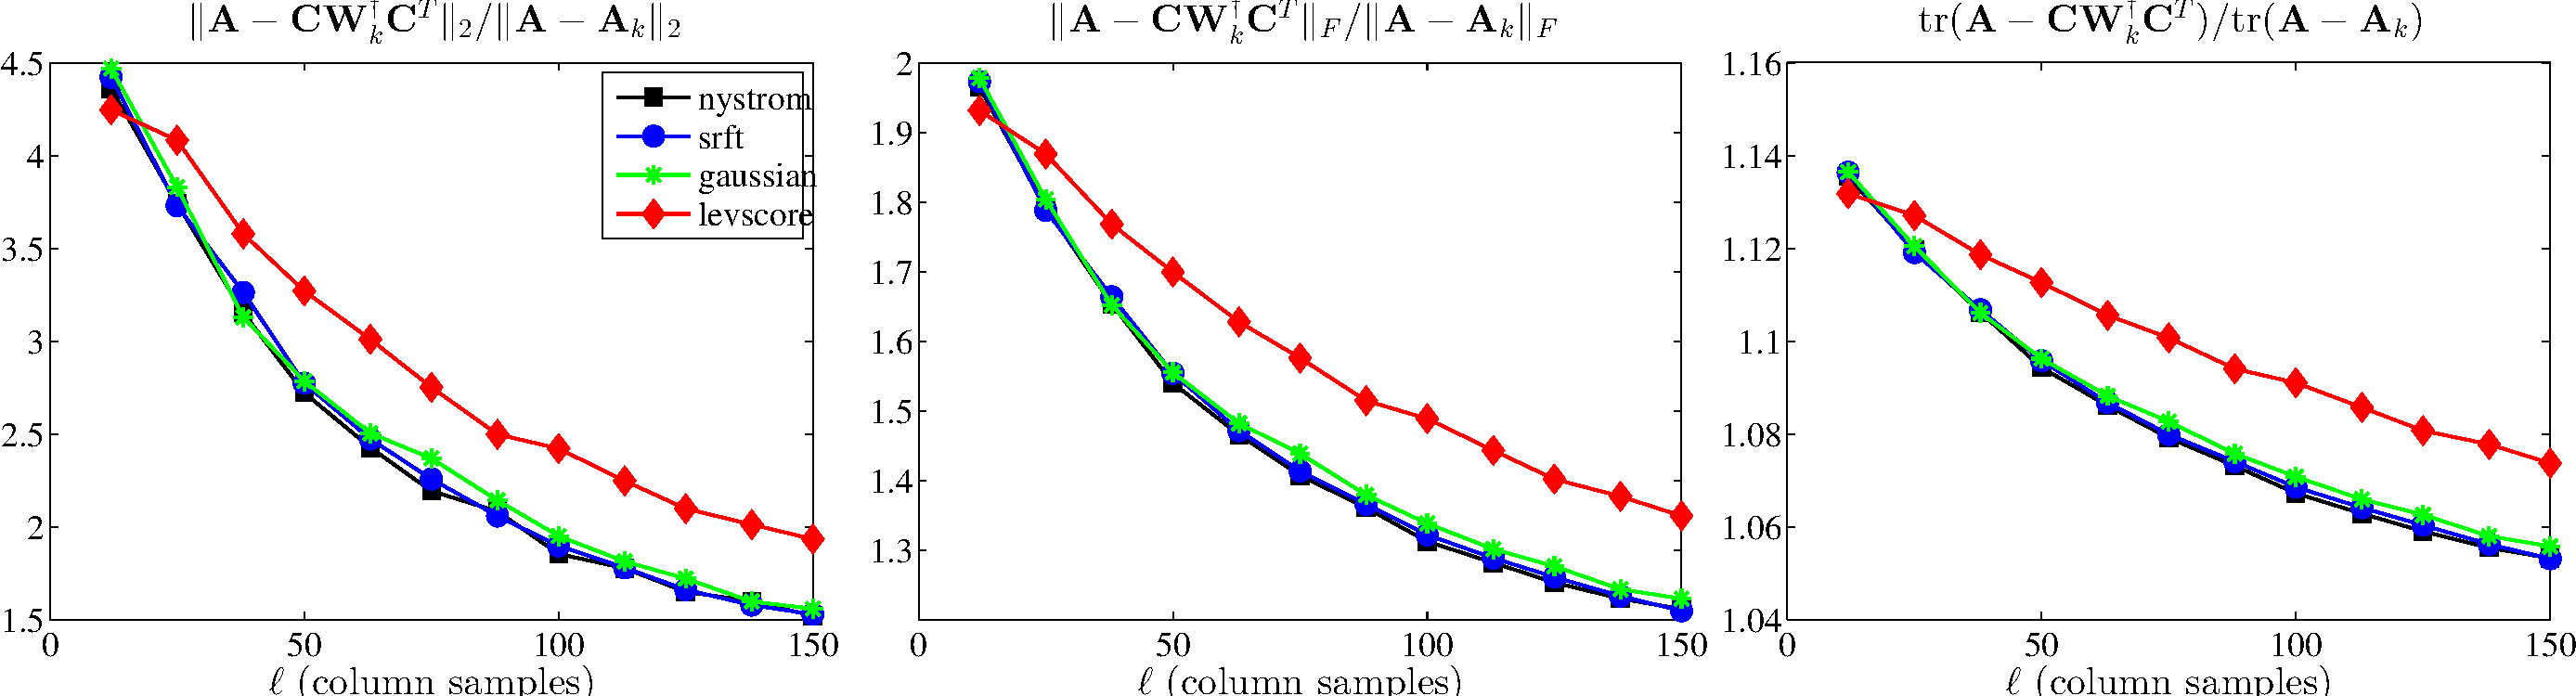
\includegraphics[width=6in, keepaspectratio=true]{figures/ch4/Gisetterank12exact-methods-fixed-rank-errors}}
 \caption[Relative errors of rank-restricted SPSD sketches of the linear kernel matrices]{%
 {\sc Relative errors of rank-restricted SPSD sketches of the linear kernel matrices.}
 The relative spectral, Frobenius, and trace-norm errors~\eqref{ch4:eqn:relerr2} of several rank-restricted
 SPSD sketches, as a function of the number of columns samples $\ell$, 
 for the linear kernel matrices. }%
 \label{ch4:fig:linearkernel-exact-errors-b}
\end{figure}

Figures~\ref{ch4:fig:linearkernel-exact-errors-a} and~\ref{ch4:fig:linearkernel-exact-errors-b}
show the reconstruction error results for sampling and mixture methods 
applied to several linear kernels.  
The matrices (Dexter, Protein, SNPs, and Gisette) are all quite low-rank 
and have fairly uniform leverage scores.
Several observations are worth making about the results presented in these 
figures.
\begin{itemize}
\item
All of the methods perform quite similarly for the non-rank-restricted 
case: all have errors that decrease smoothly with increasing $\ell$, and in 
this case there is little advantage to using methods other than uniform 
sampling (since they perform similarly and are more expensive).
Also, since the ranks are so low and the leverage scores are so uniform, the 
leverage score extension is no longer significantly distinguished by its 
tendency to saturate quickly.
\item
The scale of the vertical axes is much larger than for the Laplacian matrices,
mostly since the matrices are much better approximated by low-rank 
matrices, although the scale decreases as one goes from spectral to 
Frobenius to trace reconstruction error, as before.
\item
For SNPs and Gisette, the rank-restricted reconstruction results are 
very similar for all four methods, with a smooth decrease in error as
$\ell$ is increased, although interestingly using leverage scores is
slightly worse for Gisette.
For Dexter and Protein, the situation is more complicated: using the SRFT 
always leads to smooth decrease as $\ell$ is increased, and uniform sampling
generally behaves the same way also; Gaussian mixtures behave this way 
for Protein, but 
for Dexter Gaussian mixtures are noticably worse than SRFT and uniform 
sampling; and, except for very small values of $\ell$, leverage-based 
sampling is worse still and gets noticably worse as $\ell$ is increased.
Even this poor behavior of leverage score sampling on the linear kernels is 
notably worse than for the rank-restricted Laplacians, where there was a 
range of moderately small $\ell$ where leverage score sampling was much 
superior to other methods.
\end{itemize}
These linear kernels (and also to some extent the dense RBF kernels below
that have larger $\sigma$ parameter) are examples of relatively ``nice'' 
machine learning matrices that are similar to matrices where uniform 
sampling has been shown to perform well 
previously~\cite{TKR08,KMT09a,KMT09,KMT12}; and for these matrices our 
empirical results agree with these prior works.


\subsubsection{Dense and sparse RBF kernels}

\begin{figure}[htp]
 \centering
 \subfigure[AbaloneD, $\sigma = .15, k = 20$]{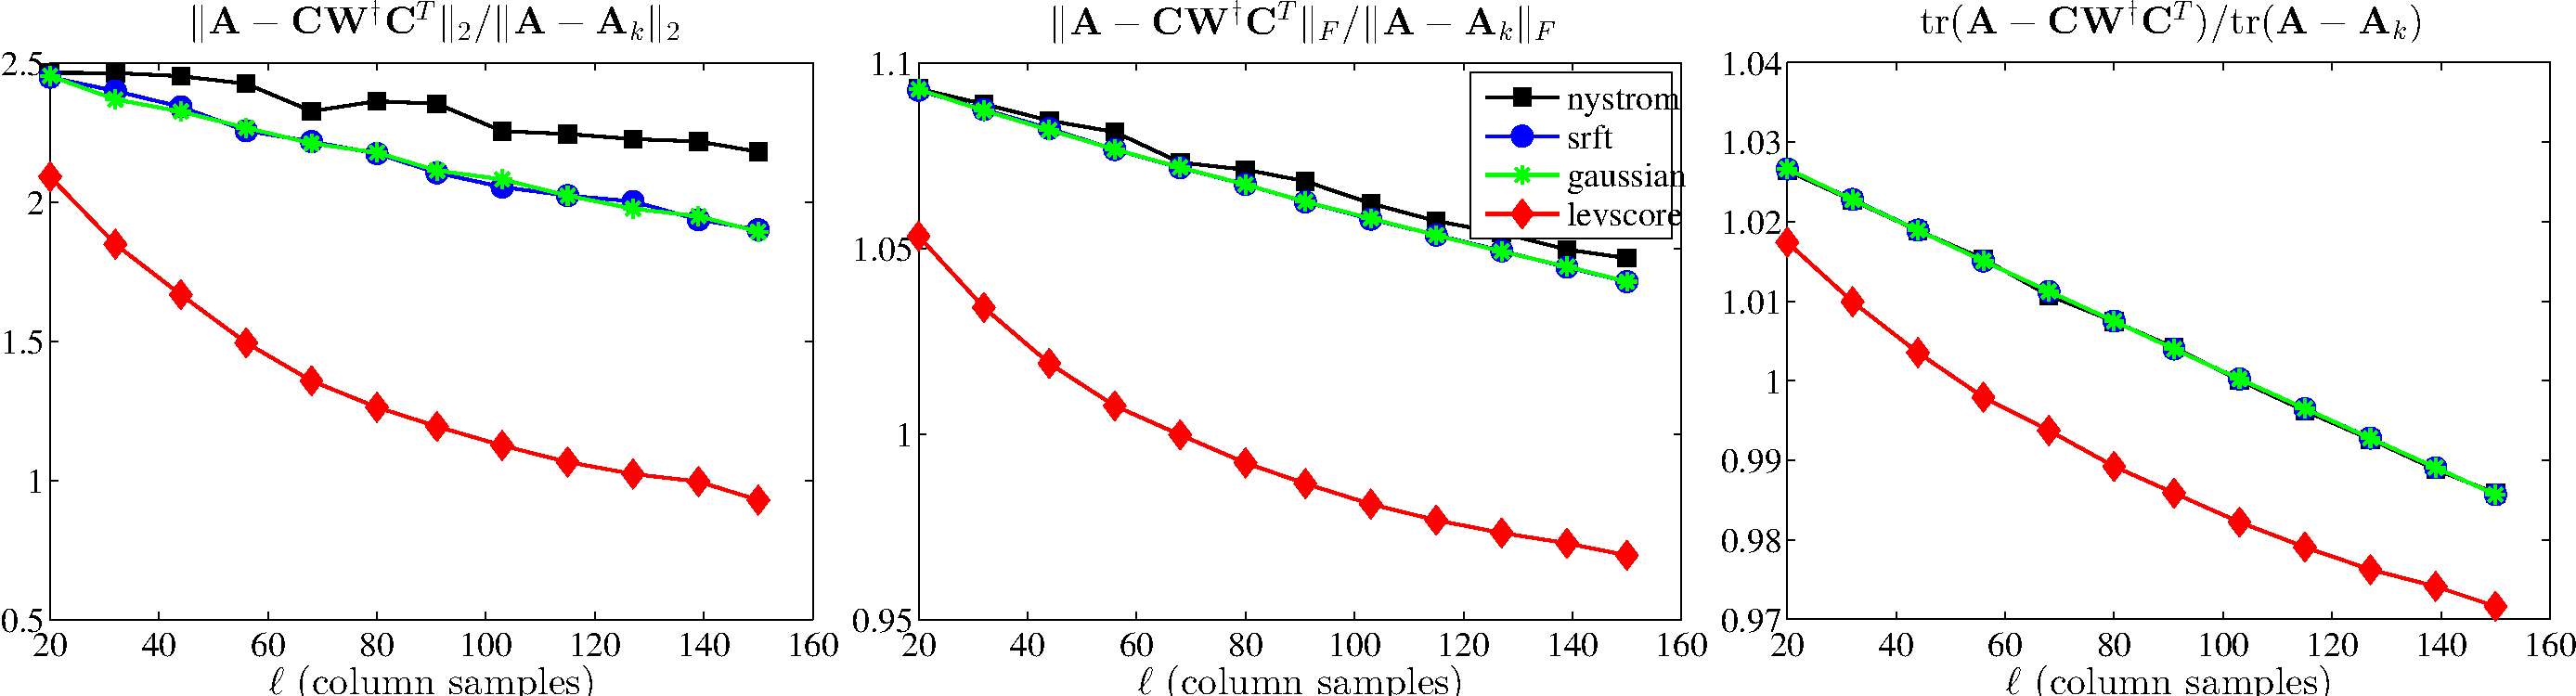
\includegraphics[width=6in, keepaspectratio=true]{figures/ch4/Abalonesigmapt15exact-methods-nonfixed-rank-errors}}
 
 \subfigure[AbaloneD, $\sigma = 1, k = 20$]{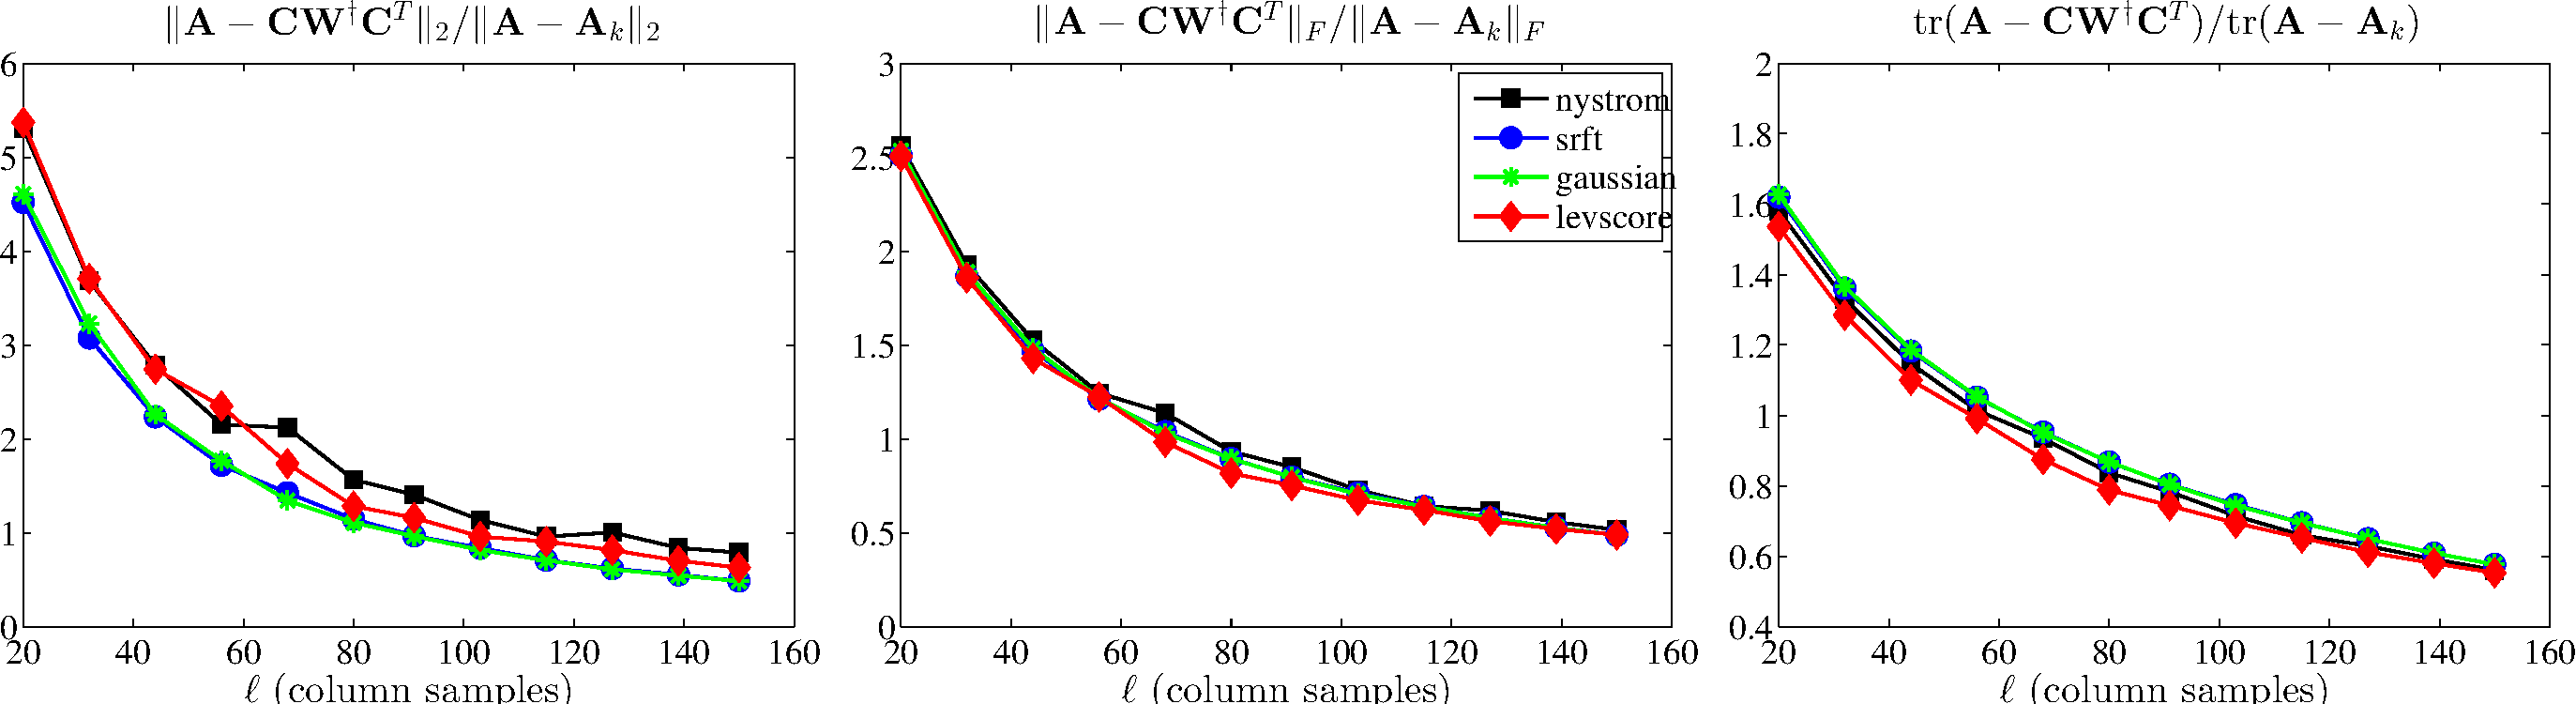
\includegraphics[width=6in, keepaspectratio=true]{figures/ch4/Abalonesigma1exact-methods-nonfixed-rank-errors}}
 
 \subfigure[WineD, $\sigma = 1, k = 20$]{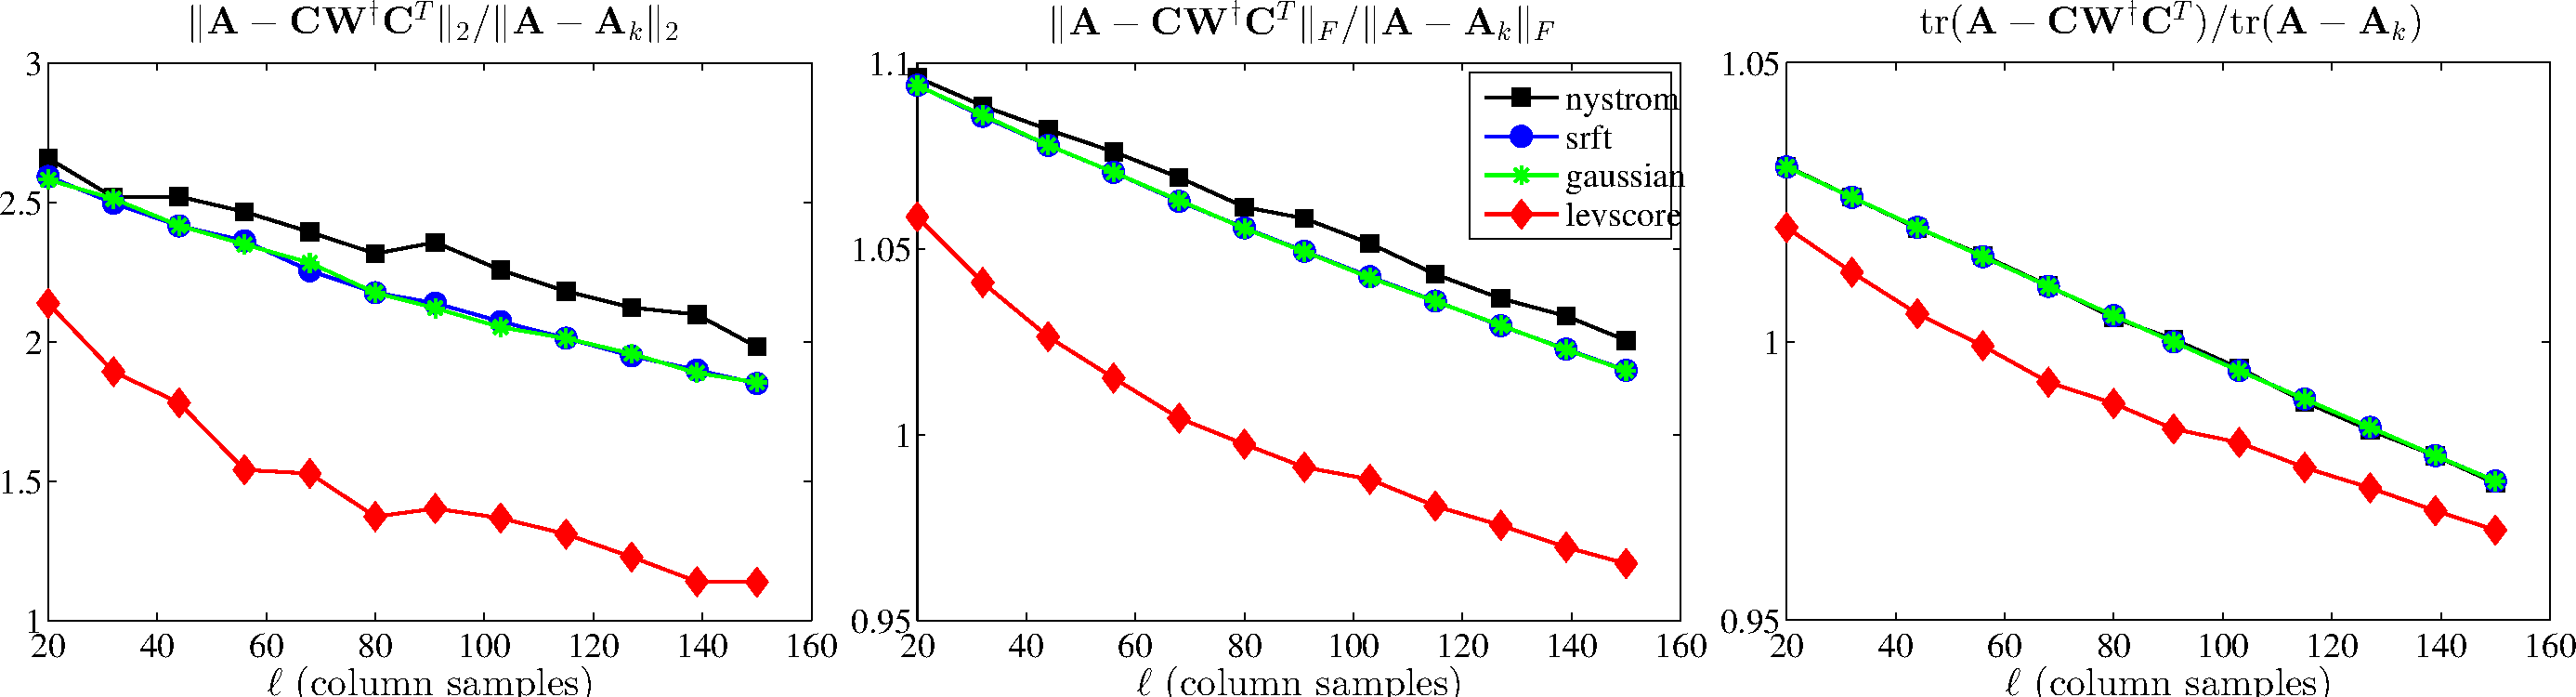
\includegraphics[width=6in, keepaspectratio=true]{figures/ch4/Winesigma1exact-methods-nonfixed-rank-errors}}
 
 \subfigure[WineD, $\sigma = 2.1, k = 20$]{\includegraphics[width=6in, keepaspectratio=true]{figures/ch4/Winesigma2pt1exact-methods-nonfixed-rank-errors}}
 \caption[Relative errors of non-rank-restricted SPSD sketches of the dense RBFK matrices]{%
 {\sc Relative errors of non-rank-restricted SPSD sketches of the dense RBFK matrices.}
 The relative spectral, Frobenius, and trace-norm errors~\eqref{ch4:eqn:relerr1} of several non-rank-restricted
 SPSD sketches, as a function of the number of columns samples $\ell$, 
 for the dense RBFK matrices. }%
 \label{ch4:fig:denserbf-exact-errors-a}
\end{figure}

\begin{figure}[htp]
 \centering
 \subfigure[AbaloneD, $\sigma = .15, k = 20$]{\includegraphics[width=6in, keepaspectratio=true]{figures/ch4/Abalonesigmapt15exact-methods-fixed-rank-errors}}
 
 \subfigure[AbaloneD, $\sigma = 1, k = 20$]{\includegraphics[width=6in, keepaspectratio=true]{figures/ch4/Abalonesigma1exact-methods-fixed-rank-errors}}
 
 \subfigure[WineD, $\sigma = 1, k = 20$]{\includegraphics[width=6in, keepaspectratio=true]{figures/ch4/Winesigma1exact-methods-fixed-rank-errors}}
 
 \subfigure[WineD, $\sigma = 2.1, k = 20$]{\includegraphics[width=6in, keepaspectratio=true]{figures/ch4/Winesigma2pt1exact-methods-fixed-rank-errors}}
 \caption[Relative errors of rank-restricted SPSD sketches of the dense RBFK matrices]{%
 {\sc Relative errors of rank-restricted SPSD sketches of the dense RBFK matrices.}
 The relative spectral, Frobenius, and trace-norm errors~\eqref{ch4:eqn:relerr2} of several rank-restricted
 SPSD sketches, as a function of the number of columns samples $\ell$, 
 for the dense RBFK matrices.}%
 \label{ch4:fig:denserbf-exact-errors-b}
\end{figure}

\begin{figure}[htp]
 \centering
 \subfigure[AbaloneS, $\sigma = .15, k = 20$]{\includegraphics[width=6in, keepaspectratio=true]{figures/ch4/Abalonecompactsigmapt15exact-methods-nonfixed-rank-errors}}
 
 \subfigure[AbaloneS, $\sigma = 1, k = 20$]{\includegraphics[width=6in, keepaspectratio=true]{figures/ch4/Abalonecompactsigma1exact-methods-nonfixed-rank-errors}}
 
 \subfigure[WineS, $\sigma = 1, k = 20$]{\includegraphics[width=6in, keepaspectratio=true]{figures/ch4/Winecompactsigma1exact-methods-nonfixed-rank-errors}}
 
 \subfigure[WineS, $\sigma = 2.1, k = 20$]{\includegraphics[width=6in, keepaspectratio=true]{figures/ch4/Winecompactsigma2pt1exact-methods-nonfixed-rank-errors}}
 \caption[Relative errors of non-rank-restricted SPSD sketches of the sparse RBFK matrices]{%
 {\sc Relative errors of non-rank-restricted SPSD sketches of the sparse RBFK matrices.}
 The relative spectral, Frobenius, and trace-norm errors~\eqref{ch4:eqn:relerr1} of several non-rank-restricted
 SPSD sketches, as a function of the number of columns samples $\ell$, 
 for the sparse RBFK matrices.}%
 \label{ch4:fig:sparserbf-exact-errors-a}
\end{figure}

\begin{figure}[htp]
 \centering
 \subfigure[AbaloneS, $\sigma = .15, k = 20$]{\includegraphics[width=6in, keepaspectratio=true]{figures/ch4/Abalonecompactsigmapt15exact-methods-fixed-rank-errors}}
 
 \subfigure[AbaloneS, $\sigma = 1, k = 20$]{\includegraphics[width=6in, keepaspectratio=true]{figures/ch4/Abalonecompactsigma1exact-methods-fixed-rank-errors}}
 
 \subfigure[WineS, $\sigma = 1, k = 20$]{\includegraphics[width=6in, keepaspectratio=true]{figures/ch4/Winecompactsigma1exact-methods-fixed-rank-errors}}
 
 \subfigure[WineS, $\sigma = 2.1, k = 20$]{\includegraphics[width=6in, keepaspectratio=true]{figures/ch4/Winecompactsigma2pt1exact-methods-fixed-rank-errors}}
 \caption[Relative errors of rank-restricted SPSD sketches of the sparse RBFK matrices]{%
 {\sc Relative errors of rank-restricted SPSD sketches of the sparse RBFK matrices.}
 The relative spectral, Frobenius, and trace-norm errors~\eqref{ch4:eqn:relerr2} of several rank-restricted
 SPSD sketches, as a function of the number of columns samples $\ell$, 
 for the sparse RBFK matrices. }%
 \label{ch4:fig:sparserbf-exact-errors-b}
\end{figure}

Figures~\ref{ch4:fig:denserbf-exact-errors-a}--\ref{ch4:fig:sparserbf-exact-errors-b} 
present 
the reconstruction error results for sampling and mixture methods 
applied to several dense RBF and sparse RBF kernels.
Several observations are worth making about the results presented in these 
figures.
\begin{itemize}
\item
For the non-rank-restricted results, all of the methods have errors that 
decrease with increasing $\ell$.
In particular, for larger values of $\sigma$ and for denser matrices, the 
decrease is somewhat more regular, and the four methods tend to perform 
similarly.
For larger values of $\sigma$ and sparser matrices, leverage
score sampling is somewhat better.
This parallels what we observed with the linear kernels, except that here the 
leverage score sampling is somewhat better for all values of $\ell$.
\item
For the non-rank-restricted results for the smaller values of $\sigma$, 
leverage score sampling tends to be much better than uniform sampling and 
mixture-based methods.
For the sparse matrices, however, this effect saturates. We again observe 
(especially when $\sigma$ is smaller in AbaloneS and WineS) the tradeoff we 
observed previously with the Laplacian matrices: leverage score sampling is 
better when $\ell$ is moderately larger than $k$, while uniform sampling and 
random mixtures are better when $\ell$ is much larger than $k$.
\item
For the rank-restricted results, we see that when $\sigma$ is large, all 
of the results tend to perform similarly.
(The exception to this is WineS, for which leverage score sampling starts out 
much better than other methods and then gets worse as $\ell$ is increased.)
On the other hand, when $\sigma$ is small, the results are more complex.
Leverage score sampling is typically much better than other methods, 
although the results are quite choppy as a function of $\ell$, and in some 
cases the effect diminishes as $\ell$ is increased.
\end{itemize}
Recall from Table~\ref{ch4:table:datasets_stats} that for smaller values of 
$\sigma$ and for sparser kernels, the SPSD matrices are less 
well-approximated by low-rank matrices, and they have more heterogeneous 
leverage scores.
Thus, they are more similar to the Laplacian matrices than the linear kernel 
matrices; and this suggests (as we have observed) that leverage score sampling 
should perform better than uniform column sampling and 
mixture-based schemes in these two cases.
In particular, nowhere do we see that leverage score sampling performs much 
worse than other methods, as we saw with the rank-restricted linear 
kernel results.

\subsubsection{Summary of comparison of sampling and mixture-based SPSD Sketches}

Several summary observations can be made about sampling versus mixture-based SPSD sketches
for the matrices we have considered.
\begin{itemize}
\item
Linear kernels and to a lesser extent dense RBF kernels with larger $\sigma$
parameter have relatively low rank and relatively uniform leverage scores, 
and in these cases uniform sampling does quite well.
These matrices correspond most closely with those that have been studied 
previously in the machine learning literature, and for these matrices our 
results are in agreement with that prior work.
\item
Sparsifying RBF kernels and/or choosing a smaller $\sigma$ parameter tends
to make these kernels worse approximated by low-rank matrices and to 
have more heterogeneous leverage scores.
In general, these two properties need not be directly related: the spectrum is 
a property of eigenvalues, while the leverage scores are determined by the 
eigenvectors. However, in the matrices we examined they are related, in that 
matrices with more slowly decaying spectra also often have more 
heterogeneous leverage scores.
\item
For dense RBF kernels with smaller $\sigma$ and sparse RBF kernels, leverage 
score sampling tends to do much better than other methods.
Interestingly, the sparse RBF kernels have many properties of very sparse 
Laplacian kernels corresponding to relatively unstructured informatics 
graphs.

\item
Reconstruction quality under leverage score sampling saturates, as a 
function of choosing more samples $\ell$; this is seen both for 
non-rank-restricted and rank-restricted situations.
As a consequence, there is often a transition between leverage score sampling
or other methods being better as $\ell$ increases.
\item
Although they are potentially ill-conditioned, non-rank-restricted approximations 
behave better in terms of reconstruction quality.
Rank-constrained approximations tend to have much more complicated behavior
as a function of increasing the number of samples $\ell$, including choppier
and non-monotonic behavior.
This is particularly severe for leverage score sampling, but it occurs with
other methods. Other forms of regularization might be appropriate.
\end{itemize}
In general, \emph{all} of the sampling and mixture-based sketches we considered 
perform \emph{much} better on the SPSD matrices we considered than both the previous
worst-case bounds (e.g.,~\cite{DM05,KMT12}) 
and the bounds derived in this chapter would suggest.
Even the worst results correspond to single-digit approximation 
factors in relative scale.

\section{A comparison with projection-based low-rank approximations}
\label{ch4:sec:comparison}

\begin{figure}[tb!]
 \centering
 \subfigure[Gnutella, $k=20$]{\includegraphics[width=6in, keepaspectratio=true]{figures/ch4/Gnutellarank20-eigexact-methods-nonfixed-rank-errors-with-eig}}
 
 \subfigure[Dexter, $k=8$]{\includegraphics[width=6in, keepaspectratio=true]{figures/ch4/Dexterrank8-eigexact-methods-nonfixed-rank-errors-with-eig}}
 
 \subfigure[AbaloneD, $\sigma = .15, k = 20$]{\includegraphics[width=6in, keepaspectratio=true]{figures/ch4/Abalonesigmapt15-eigexact-methods-nonfixed-rank-errors-with-eig}}
 
 \subfigure[WineS, $\sigma=1, k=20$]{\includegraphics[width=6in, keepaspectratio=true]{figures/ch4/Winecompactsigma1-eigexact-methods-nonfixed-rank-errors-with-eig}}
 \caption[Comparison of projection-based low-rank approximations with one-pass SPSD sketches]{%
 {\sc Comparison of projection-based low-rank approximations with one-pass SPSD sketches.}
 The relative spectral, Frobenius, and trace-norm errors~\eqref{ch4:eqn:relerr1} of several
 non-rank-restricted SPSD sketches, including the pinched and prolonged low-rank approximants, 
 as a function of the number of columns samples $\ell$, 
 for several matrices from Table~\ref{ch4:table:datasets}. }%
 \label{fig:pinched-and-prolonged-approximants}
\end{figure}

Finally, we consider the performance of two projection-based SPSD sketches 
proposed in~\cite{HMT11}. Recall from Chapter~\ref{ch3} that these
low-rank approximations are constructed by forming an approximate basis $\matQ$ for 
the top $k$-dimensional eigenspace of $\matA$ and then restricting $\matA$ to that eigenspace. 

Given a sampling matrix $\matS,$ form the matrix 
$\matY = \matA \matS$ and take the QR decomposition of $\matY$ to obtain 
$\matQ,$ a matrix with orthonormal columns. The first projection-based approximant
mentioned in~\cite{HMT11}, which we eponymously refer to as the \emph{pinched} approximant, is simply $\matA$ pinched 
to the space spanned by $\matQ:$ 
\[
 \matP_{\matA \matS} \matA \matP_{\matA \matS} = \matQ (\matQ\transp \matA \matQ\transp) \matQ.
\]
Note that this approximant requires two passes over $\matA$. The second approximant, which 
we refer to as the \emph{prolonged} approximant, is 
\[
\matA \matQ (\matQ\transp \matA \matQ)^\pinv \matQ\transp \matA.
\]
The computation of a prolonged approximant also requires two passes over $\matA.$

It is clear that the prolonged approximant can be constructed using our SPSD 
sketching model by taking $\matQ$ as the sketching matrix. In fact, a stronger
statement can be made. Recall, from Lemma~\ref{ch4:lem:proj-form-of-sketch},
that for any sketching matrix $\matX,$ when 
$\matC = \matA \matX$ and $\matW = \matX\transp \matA \matX,$
\[
 \matC \matW^\pinv \matC\transp = 
 \matA^{1/2} \matP_{\matA^{1/2} \matX} \matA^{1/2}.
\]
By considering the two choices $\matX = \matA \matS$ and $\matX = \matQ$, we 
see that in fact the prolonged approximant is exactly the two-pass SPSD sketch:
\begin{align*}
 \matA \matQ ( \matQ\transp \matA \matQ)^\pinv \matA \matQ & = 
 \matA^{1/2} \matP_{\matA^{1/2} \matQ} \matA^{1/2} \\
 & = \matA^{1/2} \matP_{\matA^{1/2} (\matA \matS) } \matA^{1/2} \\
 & = \matA^2 \matS (\matS\transp \matA^3 \matS)^\pinv\matS\transp \matA^2.
\end{align*}
It follows that the bounds we provide in Section~\ref{ch4:sec:structuralresults} on the 
performance of multi-pass sketches pertain also to 
prolonged approximants. In particular, the additional errors of these approximants
are expected to be at least a factor of $\lambda_{k+1}(\matA)/\lambda_k(\matA)$
smaller than the additional errors of one-pass sketches.

In Figure~\ref{fig:pinched-and-prolonged-approximants}, we compare the empirical 
performances of several of the SPSD sketches considered earlier with  
pinched and prolonged approximants constructed using the same matrix $\matS.$
Specifically, we plot the errors of
pinched and prolonged approximants for choices of sketching
matrices corresponding to uniform column sampling, gaussian column 
mixtures, and SRFT-based column mixtures, along with the errors of one-pass
SPSD sketches constructed using the same choices of $\matS.$ In the
interest of brevity, we provide results only for a subset of the matrices 
listed in Table~\ref{ch4:table:datasets} and consider only the nonfixed-rank 
variants of the sketches.

Some trends are clear from Figure~\ref{fig:pinched-and-prolonged-approximants}.
\begin{itemize}
\item In the spectral norm, the prolonged approximants are considerably more accurate 
than the pinched approximants and one-pass sketches for all the matrices considered. Without 
exception, the prolonged Gaussian and SRFT column-mixture approximants are the most accurate
in the spectral norm, of all the schemes considered. Only in the case of the 
Dexter linear kernel is the prolonged uniformly column-sampled approximant nearly as
accurate in the spectral norm as the prolonged Gaussian and SRFT approximants. To
 a lesser extent, the prolonged approximants are also more accurate in the Frobenius
 and trace norms than the other schemes considered. The increased Frobenius and
 trace norm accuracy is particularly notable for the two RBF kernel matrices;
 again, the prolonged Gaussian and SRFT approximants are considerably more accurate
 than the prolonged uniformly column-sampled approximants.  
 \item After the 
 prolonged approximants, the pinched Gaussian and SRFT column-mixture approximants 
 have the smallest spectral, Frobenius, and trace-norm 
 errors. Again however, we see that the pinched uniformly column-sampled 
 approximants are considerably less accurate than the
 pinched Gaussian and SRFT column-mixture approximants. Particularly in the 
 spectral and Frobenius norms, the pinched uniformly column-sampled approximants
 are not any more accurate than the uniformly column-sampled sketches.
 \end{itemize}
It is evident that the benefits of pinched and
prolonged approximants are most dramatic when the spectral norm is the error metric,
and that Nystr\"om extensions do not benefit as much from multiple passes as do other
sketching schemes.

It is also evident that the pinched approximants
often yield a much slighter increase in accuracy over the one-pass sketches than do the
prolonged approximants. Recall that the prolonged approximants are simply
two-pass sketches. Our investigations point to the conclusion that two-pass sketches
are significantly more accurate than the projection-based low-rank approximations
that also require two passes over $\matA.$ Of course, one should temper this
comparison with the knowledge that projection-based low-rank approximations, unlike SPSD sketches, are stably computable.


\bibliographystyle{amsalpha}
\bibliography{thesisbib}
\end{document}
